\chapter{Introduction to Liferay DXP
Deployment}\label{introduction-to-liferay-dxp-deployment}

Liferay DXP is one of the most flexible applications on the market today
with respect to database and application server support. Liferay DXP
supports a wide variety of databases and application servers, freeing
you to use the ones you think are best. Liferay DXP also scales very
well. You can install Liferay DXP on a shared hosting account, on a
multi-node cluster running a commercial application server, or on
anything in between. In fact, Liferay DXP is used successfully in all of
these scenarios every day.

\section{Supported Platforms and
Limitations}\label{supported-platforms-and-limitations}

The list of supported OSes, application servers, databases, and other
environments is always available on the Customer Portal at
\url{https://www.liferay.com/group/customer} under the Support Matrix
links.

Applications developed by Liferay, such as Audience Targeting, are
available through the Liferay
\href{https://www.liferay.com/marketplace/}{Marketplace}. It's possible
that some of these applications are supported only on certain
environments. This is always specified in the application's description.
If you are planning to use these additional products, make sure Liferay
DXP is running on a supported environment before installing one of these
applications.

\section{Reference Architecture}\label{reference-architecture}

When considering deploying Liferay DXP, selecting the right architecture
is one of the first decisions you need to make. You need to consider
these factors:

\begin{itemize}
\tightlist
\item
  Information Security: Securing sensitive hardware and information from
  malicious attack and intrusion
\item
  Performance: Supporting the desired number of total users, concurrent
  transactions, etc.
\item
  Fault Tolerance: Maintaining uptime during unexpected failure or
  scheduled maintenance
\item
  Flexibility and Scalability: Designing an expandable architecture to
  support additional features and users without significant redesign
\end{itemize}

The reference architecture depicted in Figure 1 provides high levels of
fault tolerance and flexibility.

\begin{figure}
\centering
\includegraphics{./images-dxp/de-reference-architecture.png}
\caption{The 7.0 reference architecture is scalable.}
\end{figure}

The architecture contains the following tiers:

\begin{itemize}
\tightlist
\item
  \textbf{Firewall:} Intrusion detection and prevention
\item
  \textbf{Load Balancer Tier}: Ensures smooth distribution of load
  between multiple web server resources
\item
  \textbf{Web Server Tier}: Delivers static content like images, rich
  media, CSS files, etc. Also provides integration modules to single
  sign-on solutions like CA SiteMinder, Oracle Identity, Ping, etc.
\item
  \textbf{Application Tier:} Hosts Liferay DXP supported application
  servers like Tomcat, JBoss, Oracle Weblogic, and IBM WebSphere (please
  see 7.0 Compatibility Matrix for additional platforms). Also hosts
  search engines like Solr and Elasticsearch.
\item
  \textbf{Database Tier:} Hosts Liferay DXP supported database servers
  like MySQL, Oracle, MS SQL Server, IBM DB2, PostgreSQL (please see 7.0
  Compatibility Matrix for additional platforms)
\end{itemize}

The hardware deployed within each tier varies depending on the type of
transactions.

\subsection{Virtualized and Cloud
Deployments}\label{virtualized-and-cloud-deployments}

While the reference architecture describes a physical deployment, the
same concepts may be applied to a cloud based or virtualized deployment.
Many Liferay DXP customers choose to deploy on public clouds
(e.g.~Amazon EC2) or their own private clouds (e.g.~VMWare VSX based
private cloud). Physical machines can be replaced by appropriate
quantities of virtual machines.

In virtualized deployments, it is critical to allocate sufficient CPU
resources. For instance, for systems deployed to Amazon AWS, allocated
CPUs are calculated using Amazon EC2 Compute Units. However, 1 Compute
Unit does not equal to 1 physical CPU or even 1 core on a CPU. In
Amazon's terms, each application server equates to roughly a ``Cluster
Compute Quadruple Extra Large Instance,'' or 33.5 EC2 Compute Units.
Thus, to plan the virtualized / cloud deployment properly, customers
must account not only for virtualization overhead, but also for
allocation of sufficient CPU resources.

\subsection{Fault Tolerance}\label{fault-tolerance}

The reference architecture is fault tolerant at every level. With
clusters at the web, application, and database tier, you may suffer a
catastrophic hardware failure of any node and continue to serve users
with little performance degradation.

The depicted reference architecture represents the minimum deployment
units to ensure proper fault tolerance within a single data center. You
may increase the number of servers within each tier according to your
load patterns to achieve a multiplier effect in the number of users the
deployment can support while maintaining sufficient fault tolerance.

Multi-data-center fault tolerant architectures are not provided as part
of the reference architecture.

\subsection{Performance}\label{performance}

Each deployment's performance characteristics vary depending on the type
of activity and the performance of custom application elements. Liferay
Engineering has created a series of scenarios to benchmark 7.0's out of
the box performance characteristics for content management,
collaboration and social enterprise scenarios. Results from these
reference architectures have indicated 7.0 can support over 22,000
virtual collaboration users and over 150,000 logins per minute with an
average login time of 300 milliseconds. 7.0 accomplished this load
within the reference architecture while using no more than 40\% of CPU
resources in the Web Tier, 86\% of CPU resources in the Application
Tier, and 50\% of CPU resources in the Database Tier.

\subsection{Scalability}\label{scalability}

Liferay Engineering's testing has shown 7.0 to scale linearly. Thus, if
you know a single application server supports X virtual users and
assuming sufficient database and web server resources, you may calculate
the total number of application servers required.

\subsection{Security}\label{security}

The firewall preceding the Load Balancer Tier provides sufficient
intrusion detection and prevention. However, depending on your
organization's information security requirements, you may introduce
additional firewall layers between each tier to further secure the
infrastructure.

\subsection{Environment Types}\label{environment-types}

Before starting to plan your Liferay DXP deployment, it's important to
include different environments to be able to maintain the projects.
Liferay uses the following terminology for systems:

\textbf{Development:} The environment where the software is written.
Most simply it is developer workstations containing integrated
development environments with version and dependency handling along with
a version control system with working copies on the individual developer
workstations.

\textbf{SIT (System Integration Testing):} SIT is where the systems
delivered are validated. The is an environment for testing the
automation of aggregated components and the dependencies between them.

\textbf{UAT (User Acceptance Testing):} A QA or Test environment. The
developers deploy the software here when it's ready for users to verify
its functionality.

\textbf{Production Staging:} A pre-production environment that's as
close as possible to the production environment for final testing, such
as installation, configuration, deployment and load, and performance
testing.

\textbf{Production:} The environment that's accessed directly by end
users. Because this is the live environment, updates are done using a
secure process, particularly if it is a complex clustered environment.

\chapter{Deploying Liferay DXP}\label{deploying-liferay-dxp}

Liferay DXP is one of the most flexible applications on the market today
with respect to database and application server support. Liferay DXP
supports a wide variety of databases and application servers, freeing
you to use the ones you think are best. Liferay DXP also scales very
well. You can install Liferay DXP on a shared hosting account, on a
multi-node cluster running a commercial application server, or on
anything in between. In fact, Liferay DXP is used successfully in all of
these scenarios every day. Some features, such as clustering, are only
available with Liferay's Digital Experience Platform.

You'll find that because Liferay DXP is extremely flexible in its
deployment options, it is also easy to install. If you already have an
application server, you can use your application server's deployment
tools to install Liferay DXP. If you don't already have an application
server, Liferay provides several application server bundles from which
to choose. These are pre-configured application servers with Liferay DXP
already installed on them. They're easy to install and with a small
amount of configuration can be made into production-ready systems.

Read on to learn how you can prepare to install Liferay DXP.

\section{Preparing for Install}\label{preparing-for-install}

Installing Liferay DXP is easy. But before you begin, you should answer
a few questions.

\begin{itemize}
\tightlist
\item
  Which version of Liferay will you install?
\item
  On which application server will you install Liferay DXP?
\item
  Can you install a Liferay DXP bundle or do you need to install
  Liferay DXP on an existing application server?
\item
  Which database will you use with Liferay DXP?
\item
  How do you plan to store your data?
\item
  Can your network support Liferay DXP?
\item
  Will you enable Liferay's PACL security feature?
\end{itemize}

Next, you'll answer these questions and learn the basic steps for
installing Liferay DXP.

\subsection{Obtaining Liferay DXP}\label{obtaining-liferay-dxp}

Anyone can download Liferay DXP from
\href{https://www.liferay.com}{liferay.com}. Click Platform →
\emph{Downloads}, and you'll be able to download either the open source
version of Liferay DXP or a trial of the commercial version in several
different formats. These include our convenient bundles as well as
\texttt{.war} files for installing Liferay DXP on your application
server of choice.

Liferay enterprise subscribers can download Liferay DXP from the
\href{https://help.liferay.com/hc}{Help Center}. You have a choice of
the same open source app server bundles as community members, plus a few
commercial alternatives, in addition to the \texttt{.war} files for
manual installation.

So what is a Liferay DXP bundle anyway? A Liferay DXP bundle is an
application server with Liferay DXP pre-installed. Using a bundle is the
easiest way to install Liferay DXP. Liferay DXP is bundled with a number
of application servers; all you need to do is choose the one that best
fits your needs. If you don't currently have an application server
preference, consider starting with the Tomcat bundle. Tomcat is one of
the most lightweight and straightforward bundles to configure. If you
have an open source application server preference, choose the server you
prefer from the available Liferay DXP bundles. You must have a JDK (Java
Development Kit) 8 installed prior to launching Liferay DXP.

\noindent\hrulefill

\textbf{Note:} Please see
\href{https://help.liferay.com/hc/en-us/articles/360015783792-Liferay-DXP-7-0-Compatibility-Matrix}{the
compatibility matrix} for information on supported JDKs, databases, and
environments.

\noindent\hrulefill

Please note that Liferay DXP is not able to provide application server
bundles for proprietary application servers such as WebLogic or
WebSphere, because the licenses for these servers don't allow for
redistribution. Liferay DXP's commercial offering, however, runs just as
well on these application servers as it does on the others. You'll need
to follow our manual installation procedure using a \texttt{.war} file
to install Liferay DXP on proprietary application servers.

Once you have Liferay DXP, you can plan out your installation. First,
determine if you need Liferay DXP Security turned on. Second, prepare
your database. Third, install Liferay DXP. Fourth, configure your network.
Fifth, configure search. You can install Liferay DXP either by using a
bundle or by installing it manually on your existing application server.
Next, we'll go over the steps it takes to install Liferay DXP.

\subsection{Liferay DXP Installation
Steps}\label{liferay-dxp-installation-steps}

Before you begin installing Liferay DXP, you should review these basic
installation steps:

\begin{enumerate}
\def\labelenumi{\arabic{enumi}.}
\item
  Choose a database server to use with Liferay DXP and create a new
  database. Determine whether you want Liferay DXP to manage your
  database connection or your application server to manage your database
  connection. We recommend that you let Liferay DXP manage your database
  connection. Liferay DXP can connect with several open source or
  enterprise level document repositories.
\item
  Gather mail credentials for sending email notifications to users.
  Determine whether you want Liferay DXP to manage your mail session or
  your application server to manage your mail session. Liferay DXP
  provides a built-in mail session but also supports a JNDI mail
  session. We recommend that you let Liferay DXP manage your mail
  session.
\item
  Install either a Liferay DXP bundle or install Liferay DXP on an
  existing application server (further instructions below).
\item
  Choose IPv4 or IPv6. Determine which address format is best for your
  network (further instructions below).
\item
  Determine how you'll configure Elasticsearch. Liferay DXP's default
  embedded configuration is not supported for production use, so you'll
  have to install Elasticsearch separately, either on the same
  infrastructure or on its own.
\item
  Determine whether you'll use Liferay Marketplace or other third party
  applications. If you will, you should enable Liferay's Plugin Access
  Control List (PACL) security feature.
\item
  Configure ports (optional). Liferay's application server (e.g., Tomcat
  or Wildfly) uses certain ports for purposes like handling incoming
  HTTP requests, HTTPS requests, or AJP requests, etc. If you start your
  application server in debug mode, there will be a port listening for a
  debugger to connect. If desired, you can configure these ports. Please
  refer to your application server's documentation for information on
  its default ports and how to configure them.

  Liferay also provides access to its OSGi framework through a
  configurable port:

  \texttt{module.framework.properties.osgi.console=localhost:11311}

  You can override this default property by copying the line above to
  your \texttt{LIFERAY\_HOME/portal-ext.properties} file and adjusting
  the port number.
\end{enumerate}

We'll go through the steps in order, so first we'll look at the Liferay
DXP database.

\subsection{Step 1: Choose a Database Server and Create a New
Database}\label{step-1-choose-a-database-server-and-create-a-new-database}

The recommended way of setting up your Liferay DXP database is also the
simplest. Liferay DXP takes care of just about everything. You only need
to take two simple steps:

\begin{enumerate}
\def\labelenumi{\arabic{enumi}.}
\tightlist
\item
  Create a blank database encoded with the character set UTF-8. Liferay
  DXP is a multilingual application and needs UTF-8 encoding to display
  all of its supported character sets.
\end{enumerate}

\noindent\hrulefill

\begin{verbatim}
 **Note:** If you plan to migrate from one database vendor to another,
 [configure the database to use the default query result order you expect for entities Liferay DXP lists](/docs/7-0/tutorials/-/knowledge_base/t/sort-order-changed-with-a-different-database).
\end{verbatim}

\noindent\hrulefill

\noindent\hrulefill

\begin{verbatim}
 **Note:** If you use Sybase, configure the database to allow null values by
 default.
\end{verbatim}

\noindent\hrulefill

\begin{enumerate}
\def\labelenumi{\arabic{enumi}.}
\setcounter{enumi}{1}
\tightlist
\item
  Create a database user for accessing this database. Grant this
  database user all rights, including the rights to create and drop
  tables, to the blank Liferay DXP database.
\end{enumerate}

\noindent\hrulefill

\begin{verbatim}
**Important:** Liferay requires reading from and writing to the database.
The Liferay database user must therefore have permissions to read and write
data.
\end{verbatim}

\noindent\hrulefill

Liferay DXP uses this database user's credentials to connect to the
Liferay DXP database either directly or through its application server.
During its initial startup, Liferay DXP creates the tables it needs in
the database you just created. It does this automatically, complete with
indexes.

This is the recommended way to set up Liferay DXP. It enables Liferay DXP
to maintain its database automatically during upgrades or when various
Liferay DXP plugins that create database tables of their own are
installed. This method is by far the best way to set up your Liferay DXP
database.

\noindent\hrulefill

\textbf{Warning:} If you're using an Oracle database, use the
\texttt{ojdbc8.jar} driver library with at least Oracle 12.2.0.1.0 JDBC
4.2 versioning because
\href{https://issues.liferay.com/browse/LPS-79229}{data truncation
issues} have been detected reading data from CLOB columns.

\noindent\hrulefill

If you choose to set up Liferay DXP's database with the recommended
permissions described in this section, you can skip to the next section.

\noindent\hrulefill

\textbf{Warning:} The instructions below are not ideal for Liferay DXP
installations. This procedure is documented here so that enterprises
with more restrictive standards can install Liferay DXP with stricter
(but sub-optimal) database settings. If it's at all possible, we
recommend that you use the method described in the previous section
instead of the procedure outlined below.

\noindent\hrulefill

Even though Liferay DXP can create its database automatically, some
enterprises prefer \emph{not} to allow the database user configured in
an application server to have the database permissions necessary for
Liferay DXP and its plugins to maintain their tables. For these
organizations, Select, Insert, Update and Delete are the only allowed
permissions. Thus, in this section we explain how to set up the database
manually. If your organization \emph{is} willing to grant the Liferay
DXP database user the permissions to create and drop tables in the
database--and this is the recommended configuration--then simply use the
recommended configuration described in the previous section.

\begin{enumerate}
\def\labelenumi{\arabic{enumi}.}
\item
  Create a new, blank, database for Liferay DXP.
\item
  Grant full rights to do anything to the Liferay DXP database to the
  Liferay DXP database user.
\item
  Install Liferay DXP and start it so that it automatically populates
  its database.
\item
  Once the database has been populated with the Liferay DXP tables,
  remove the permissions for creating and dropping tables from the
  Liferay DXP database user.
\end{enumerate}

There are some caveats to running Liferay DXP like this. Many Liferay DXP
plugins create new tables when they're deployed. Additionally, Liferay
DXP has an automatic database upgrade function that runs when Liferay
DXP is upgraded. If the Liferay DXP database user doesn't have enough
rights to create/modify/drop tables in the database, you must grant
those rights to the ID before you deploy one of these plugins or start
upgrading Liferay DXP. Once the tables are created or the upgrade is
complete, you can remove those rights until the next deploy or upgrade.
Additionally, your own developers might create plugins that need to
create their own tables. These are just like Liferay DXP's plugins that
do the same thing, and they cannot be installed if Liferay DXP can't
create database tables. If you wish to install these plugins, you will
need to grant rights to create tables in the database each time before
you attempt to install them.

Liferay DXP offers several configurations to store Documents and Media
files by setting the \texttt{dl.store.impl=} property. Available options
are Simple File System Store, Advanced File System Store, CMIS Store,
DBStore, JCRStore, and Amazon S3Store. In addition, Liferay DXP can be
connected to various open source and enterprise-level document
repositories. All of the repositories are connected to Liferay DXP
through hooks available on Liferay Marketplace (see below).

Once you have your database and document repository ready, you can
install Liferay DXP on your server.

\subsection{Step Two: Gather Your Mail
Credentials}\label{step-two-gather-your-mail-credentials}

Liferay DXP uses a mail server to send email notifications. As part of
the install, therefore, you will need to have credentials that Liferay
DXP can use to connect to your mail server. Specifically, you must have
the following information:

\begin{itemize}
\tightlist
\item
  Incoming POP Server and port
\item
  POP User Name
\item
  POP Password
\item
  Outgoing SMTP Server and port
\item
  SMTP User Name
\item
  SMTP Password
\item
  A list of JavaMail properties that would override a default
  configuration
\end{itemize}

Once you've gathered this information, you're ready to move on to the
next step.

\subsection{Step Three: Install}\label{step-three-install}

The next step is to install Liferay DXP. You can do this in one of two
ways: by
\href{/docs/7-0/deploy/-/knowledge_base/d/installing-product}{installing
Liferay DXP bundled with an application server}, or by
\href{/docs/7-0/deploy/-/knowledge_base/d/installing-liferay-manually}{installing
Liferay DXP manually on an existing application server}. Each Liferay
DXP installation's
\href{/docs/7-0/deploy/-/knowledge_base/d/installing-product\#liferay-home}{Liferay
Home contains several folders}.

By far the easiest way to get Liferay DXP installed is to use a bundle.
Though bundles are pre-packaged for demo purposes, it is very easy to
turn them into full, production-ready instances of Liferay DXP.

\subsection{Step Four: Network
Configurations}\label{step-four-network-configurations}

Liferay DXP supports both IPv4 and IPv6 address formats. By default,
Liferay DXP uses IPv4 addresses. If you are using IPv6, you must configure
Liferay DXP:

\begin{enumerate}
\def\labelenumi{\arabic{enumi}.}
\item
  In the application server's environment settings, set
  \texttt{-Djava.net.preferIPv4Stack=false}.
\item
  Create a \texttt{portal-ext.properties} file in your portal's Liferay
  Home directory (if one does not already exist) and set the
  \texttt{tunnel.servlet.hosts.allowed} property to the target hosts you
  want to allow (e.g., \emph{0:0:0:0:0:0:0:1}).
\end{enumerate}

\subsection{Step Five: Configure
Elasticsearch}\label{step-five-configure-elasticsearch}

Liferay DXP by default ships with an embedded version of Elasticsearch.
While this configuration works well for demo purposes, it is not
supported in a production installation. After you install Liferay DXP,
you must configure it to connect to a standalone Elasticsearch server or
cluster. Depending on the size of your installation, this standalone
instance of Elasticsearch can reside either on the same machine you have
Liferay DXP on or a different machine. For performance purposes, it is
better to install it on a separate machine.

\subsection{Step Six: Liferay Marketplace and Portal
Security}\label{step-six-liferay-marketplace-and-portal-security}

The Liferay Marketplace is an integral part of the Liferay DXP
experience. The Marketplace plugin is required to be installed on
Liferay DXP. The Marketplace plugin enables a host of features that
extend beyond just access to the online Liferay Marketplace. Some of the
key features the Marketplace plugin enables are

\begin{itemize}
\tightlist
\item
  Liferay Marketplace: direct access to our online Marketplace
\item
  App Manager: ability to install, uninstall, and update apps
\item
  Bundled Apps: easily manage apps that may come bundled with your
  Liferay DXP
\item
  Developer Apps: ability to manage apps that you're developing
\item
  License Manager: streamlined license management for your Liferay DXP
  and apps
\end{itemize}

You will want to make sure Portal Access Control Lists are enabled if
you intend to download and install apps from Marketplace. This is an
additional layer of security that defines various permissions that apps
may or may not have.

The portal installation process attempts to deploy and register the
Marketplace plugin automatically. If you're installing Liferay DXP in an
environment that would prevent this from happening, you'll have to
perform one of several workarounds.

Now that you know where you're headed, you can install Liferay DXP. If
you have decided to install Liferay DXP using a bundle, continue with
the next section. If you're installing Liferay DXP manually, skip to the
section for your application server of choice. Once you have Liferay DXP
installed manually or via a bundle, you can move on to
\href{/docs/7-0/deploy/-/knowledge_base/d/installing-elasticsearch}{configuring
search}.

\section{Installing Liferay DXP}\label{installing-liferay-dxp}

Now that you've performed the steps needed to prepare for your
installation, you're ready to install Liferay DXP! Since bundles are the
easiest way to complete an installation, all the installation steps
below assume a bundle has been installed. If you plan to install Liferay
DXP manually, please refer to the article for your app server of choice,
and then come back here to complete the configuration steps.

Now you're ready. You've created a blank database for Liferay DXP and
have gathered the credentials you need for your mail server. The next
step is to install Liferay DXP.

\subsection{Liferay Home}\label{liferay-home}

Liferay DXP bundles contain the same folder structure regardless of
application server. The top-level folder is named for the release of
Liferay DXP. This folder is called \emph{Liferay Home}. This folder is
usually the parent folder of the application server's folder. This is
why Liferay DXP bundles place the application server inside the bundle's
root folder. On a manual installation, the location of this folder
varies by application server. In a bundle, it's part of the bundle. If
you're doing a manual installation, please refer to the article covering
that app server for its location.

In the Liferay Home folder there are folders for various purposes:

\begin{itemize}
\tightlist
\item
  \hyperref[liferay-home]{Liferay Home}

  \begin{itemize}
  \tightlist
  \item
    \texttt{data}
  \item
    \texttt{deploy}
  \item
    \texttt{license}
  \item
    \texttt{logs}
  \item
    \texttt{osgi}
  \item
    \texttt{patching-tool} (Liferay Digital Enterprise 7.0 only)
  \item
    {[}Application Server{]}
  \item
    \texttt{tools}
  \item
    \texttt{work}
  \end{itemize}
\end{itemize}

\texttt{data}: This folder is used to store an embedded HSQL database,
Liferay DXP's file repository, and Liferay DXP's search indexes.
Liferay DXP is initially configured to use the embedded HSQL database but
the HSQL database is primarily intended for demonstration and trial
purposes.
\href{@platform-ref@/7.0-latest/propertiesdoc/portal.properties.html\#JDBC}{Portal
property \texttt{jdbc.default.url}} sets the Hypersonic embedded HSQL
database location.

\texttt{deploy}: To auto-deploy Liferay DXP plugins, copy them to this
folder. Legacy style \texttt{.war} files, 7.0 style \texttt{.jar} files,
and \texttt{.lpkg} files from Liferay Marketplace are supported.
\href{@platform-ref@/7.0-latest/propertiesdoc/portal.properties.html\#Auto\%20Deploy}{Portal
property \texttt{auto.deploy.deploy.dir}} sets the auto-deploy location.

\texttt{license}: Liferay DXP's copyright and version files are here.

\texttt{logs}: This folder contains Liferay DXP's log files. The
information in Liferay DXP's log files can be quite valuable for system
administrators, especially when trying to diagnose a problem.
\texttt{portal-impl.jar}'s
\texttt{portal-impl/src/META-INF/portal-log4j.xml} file sets the
location for the log files. To override the log file location, you must
\href{/docs/7-0/tutorials/-/knowledge_base/t/advanced-customization-with-ext-plugins\#using-advanced-configuration-files}{use
an \texttt{ext-impl/src/META-INF/portal-log4j-ext.xml} file in an Ext
plugin}.

\texttt{osgi}: All the JAR files and a few configuration files for
Liferay DXP's OSGi runtime belong in this folder.
\href{@platform-ref@/7.0-latest/propertiesdoc/portal.properties.html\#Module\%20Framework}{Portal
property \texttt{module.framework.base.dir}} sets the OSGi folder
location. Here are its subfolders:

\begin{itemize}
\tightlist
\item
  \texttt{configs}: Component configuration files go here
\item
  \texttt{core}: Liferay DXP's core modules
\item
  \texttt{marketplace}: Marketplace applications and application suites
\item
  \texttt{modules}: Modules you've deployed
\item
  \texttt{portal}: Liferay DXP's non-core modules
\item
  \texttt{state}: Contains OSGi internal state files for such things as
  OSGi bundle installation, bundle storage, and more
\item
  \texttt{target-platform}: Target platform index
\item
  \texttt{test}: Modules that support test integration
\item
  \texttt{war}: WAR plugins you've deployed
\end{itemize}

\texttt{patching-tool}: This folder contains patches for Liferay DXP and
files for installing the patches (Digital Enterprise 7.0 only).

\texttt{tools}: For portal upgrade and target platform indexer.

\texttt{work}: Module Jasper work files.

\textbf{{[}Application Server{]}:} The name of this folder is different
depending on the bundle you're using. This folder contains the
application server in which Liferay DXP has been installed.

If Liferay DXP is unable to create the resources it needs in the Liferay
Home folder or if it finds itself running on certain application
servers, it creates a folder called \texttt{liferay} in the home folder
of the operating system user that is running Liferay DXP. In this case,
the \texttt{liferay} folder becomes Liferay Home. For example, if the
operating system user's name was jbloggs, the Liferay Home folder could
be \texttt{/home/bloggs/liferay} or
\texttt{C:\textbackslash{}Users\textbackslash{}jbloggs\textbackslash{}liferay}.

\subsection{Extracting a Liferay DXP
Bundle}\label{extracting-a-liferay-dxp-bundle}

Getting a Liferay DXP bundle up and running is as easy as uncompressing
the archive, possibly copying a JDBC driver, and then starting the
application server. Let's use the Liferay DXP Tomcat bundle as an
example.

\begin{enumerate}
\def\labelenumi{\arabic{enumi}.}
\item
  Unzip your Liferay DXP bundle.
\item
  If you're setting up Liferay DXP to be an actual server, copy your
  database's JDBC driver \texttt{.jar} file to
  \texttt{{[}Tomcat{]}/lib/ext}. If you're using a supported open source
  database or if you're setting up Liferay DXP for demo purposes, you
  can skip this step.
\end{enumerate}

That's it! You've extracted Liferay DXP, and it's ready for use. This is
much easier than doing a manual installation on an app server. If,
however, that's what you need to do, please at this point click the link
on the left and go through the installation procedure for your app
server of choice. When you're finished with the installation (and before
you've started Liferay DXP for the first time), come back to this spot,
because you need to hook it up to your database.

\subsection{Connecting Liferay DXP to Your
Database}\label{connecting-liferay-dxp-to-your-database}

You can connect Liferay DXP through either your app server's data source
or the one that ships with Liferay DXP. Because of its suitability for
tuning, it is recommended that you use the data source that ships with
Liferay DXP. To do this, you'll create a configuration file called
\texttt{portal-ext.properties}, and you'll place that file in your
Liferay Home folder.

The configuration varies by database, of course, so templates for each
one are provided in the
\href{/docs/7-0/deploy/-/knowledge_base/d/database-templates}{reference
section}. To connect your database, therefore, create a text file called
\texttt{portal-ext.properties} in your Liferay Home folder. Copy the
relevant template for your database and paste it into this file.

Now all you have to do is customize it. Enter the proper host name and
user and password credentials for your database, and then save the file.

\subsection{Running Liferay DXP for the First
Time}\label{running-liferay-dxp-for-the-first-time}

Next, start your app server, or start the Liferay DXP app in your app
server. For example, if you're using the Liferay DXP-Tomcat bundle,
start Tomcat as if you had downloaded it manually. Tomcat is launched by
invoking a script which is found in its \texttt{bin} folder. If you open
a command prompt or terminal and go to this folder, you can launch
Tomcat via the following command on Windows:

\begin{verbatim}
startup
\end{verbatim}

or the following command on Linux/Mac/Unix:

\begin{verbatim}
./startup.sh
\end{verbatim}

The Liferay DXP Tomcat bundle then starts. If you are on Windows,
another command prompt window appears with Tomcat's console in it. If
you are on Linux, you can see the Tomcat console by issuing the
following command:

\begin{verbatim}
tail -f ../logs/catalina.out
\end{verbatim}

Liferay DXP writes log files to folder
\texttt{{[}Liferay\ Home{]}/logs}.

The first time Liferay DXP starts, it'll take a while to create all of
its database tables. Once it has successfully started, it automatically
launches a web browser that displays Liferay DXP's Basic Configuration
page. If for some reason your browser doesn't load the Basic
Configuration page, launch your web browser and navigate to
\url{http://localhost:8080}.

\subsection{Using Liferay DXP's Setup
Wizard}\label{using-liferay-dxps-setup-wizard}

Liferay DXP's Setup Wizard runs when you start Liferay DXP for the first
time. To make it easy to configure Liferay DXP, the first thing you see
when browsing to your newly installed Liferay DXP bundle is a setup
wizard. The title of the setup wizard page is Basic Configuration. This
page provides a convenient way to make an initial Liferay DXP
configuration.

There are two sections of the wizard: the portal and the administrator.
For the portal, you need to supply the following information:

\textbf{Portal Name:} the name of the portal you're powering with
Liferay DXP.

\textbf{Default Language:} choose the default locale of your portal.

\textbf{Time Zone:} select your Liferay DXP instance's default time
zone.

For the administrator, you need to supply the following information:

\textbf{First Name:} the first name of the default administrator user

\textbf{Last Name:} the last name of the default administrator user

\textbf{Email:} the email address of the default administrator user

\noindent\hrulefill

\textbf{Note:} the administrator user's email domain is used as the
Liferay DXP instance's default domain (i.e., the
\href{@platform-ref@/7.0-latest/propertiesdoc/portal.properties.html\#Company}{\texttt{company.default.web.id}}
portal property).

\noindent\hrulefill

\begin{figure}
\centering
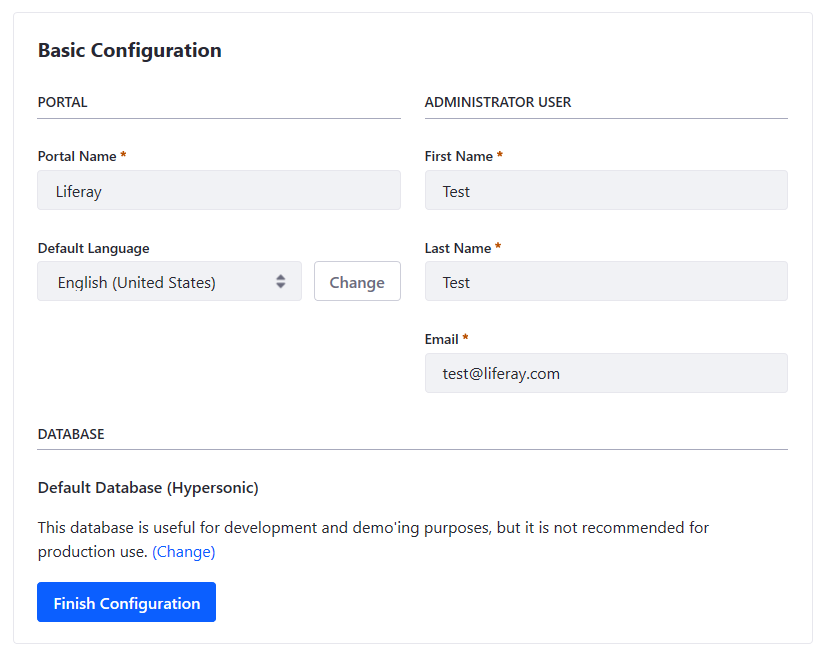
\includegraphics{./images/basic-configuration1.png}
\caption{Supply the information for your portal and your portal's
default administrator user on the Basic Configuration page.}
\end{figure}

The Basic Configuration page also includes a checkbox labeled \emph{Add
Sample Data}. If you check this box, sample data is added to Liferay
DXP's database. This data includes users, sites, and organizations. The
sample data allows many Liferay DXP features to be showcased. If you're
installing Liferay DXP on your own machine to explore its features, the
sample data will probably be useful. If, however, you're installing
Liferay DXP on a real server, you should start with a clean system.

Once you've filled out the form, click \emph{Finish Configuration}. The
setup wizard creates a \texttt{portal-setup-wizard.properties} file
which stores the settings that you entered. When you begin customizing
your portal's configuration, however, you should use the
\texttt{portal-ext.properties} file you created earlier. All the
possible properties that can be placed in this file are documented in
\href{@platform-ref@/7.0-latest/propertiesdoc}{our reference
documentation}.

\noindent\hrulefill

\textbf{Tip:} The wizard is an extremely helpful tool, especially if
you're setting up Liferay DXP for the first time. If you're a Liferay DXP
veteran and you already have your various properties set up, you can
disable the setup wizard. If you disable the setup wizard, you must
configure everything manually from the \texttt{portal-ext.properties}
file. To disable the setup wizard, enter
\texttt{setup.wizard.enabled=false} in your
\texttt{portal-ext.properties} file. Note that property values in
\texttt{portal-setup-wizard.properties} (the file created in Liferay
Home by the setup wizard) override property values in
\texttt{portal-ext.properties}.

\noindent\hrulefill

After you've entered the information requested by the Basic
Configuration page, Liferay DXP should bring you to its home page. You
should set up your mail configuration next.

\subsection{Configuring Mail}\label{configuring-mail}

Now that Liferay DXP is up and running, log in as the administrative
user you created in the setup wizard. Click the menu icon and then go to
Control Panel → Server Administration → Mail, and have your mail
credentials ready.

Fill out the form. You're asked for the following information:

\textbf{Incoming POP Server:} The hostname for a server running the Post
Office Protocol. Liferay DXP checks this mailbox for incoming messages,
such as message board replies.

\textbf{Incoming Port:} The port on which the POP server is listening.

\textbf{Use a Secure Network Connection:} Use an encrypted connection
when connecting to the POP server.

\textbf{User Name:} The user ID Liferay DXP should use to log into the
POP server.

\textbf{Password:} The password Liferay DXP should use to log into the
POP server.

\textbf{Outgoing SMTP Server:} The hostname for a server running the
Simple Mail Transfer Protocol. Liferay DXP uses this server to send
emails, such as password change emails and other notifications.

\textbf{Outgoing Port:} The port on which the SMTP server is listening.

\textbf{Use a Secure Network Connection:} Use an encrypted connection
when connecting to the SMTP server.

\textbf{User Name:} The user ID Liferay DXP should use to log into the
SMTP server.

\textbf{Password:} The password Liferay DXP should use to log into the
SMTP server.

\textbf{Manually specify additional JavaMail properties to override the
above configuration:} If there are additional properties you need to
specify, supply them here.

When you're finished setting up your mail configuration, click
\emph{Save}.

Your next step for basic Liferay DXP configuration is to convert the
search implementation from its default demo mode into a production-ready
mode.

\section{Installing Liferay DXP
Manually}\label{installing-liferay-dxp-manually}

The easiest way to install Liferay DXP is to
\href{/docs/7-0/deploy/-/knowledge_base/d/installing-product}{use a
Liferay DXP bundle}. However, this is not always possible. Some
organizations have an existing infrastructure into which Liferay DXP
must be installed. Other organizations have standardized on a particular
application server. Liferay DXP has been designed to work well with many
leading application servers. Even if you have to manually install
Liferay DXP on an existing application server, the procedure is
straightforward. Before you get started, note that there are two
distinct approaches to managing Liferay DXP's data source and mail
session. Let's review these options.

\subsection{Using Data Sources}\label{using-data-sources}

Liferay DXP provides two ways to configure your data source:

\begin{itemize}
\tightlist
\item
  Use Liferay DXP's built-in data source
\item
  Use your application's server's JNDI data source
\end{itemize}

Liferay DXP recommends that you use the built-in data source.
Liferay DXP's data source is configured by a number of properties that are
set in a properties file. By default, you can enter database connection
information on the Basic Configuration page that appears when Liferay
DXP starts for the first time. The setup wizard stores the information
you entered in a configuration file called
\texttt{portal-setup-wizard.properties} in your Liferay Home folder.
Liferay DXP's built-in data source uses this information to connect to
the database.

Although Liferay DXP recommends that you use the built-in data source,
that's not the only option. Some organizations prefer to use the data
source provided by their application server of choice. In this case, a
JNDI lookup provides a handle to the data source and the application
server manages the connection pools. So you can configure Liferay DXP to
use your application server's data source, if that's desired.

To do this, you'll need to create your own configuration file and skip
the setup wizard. Since you'd be creating this file \emph{after} the
wizard anyway, this isn't such a big deal. We show you how to configure
a JNDI data source in the Manual Configuration section below.

Since mail sessions are configured similarly to data sources, we'll look
at them next.

\subsection{Using Mail Sessions}\label{using-mail-sessions}

As with databases, you have two ways to configure your mail server:

\begin{itemize}
\tightlist
\item
  Use Liferay DXP's built-in mail session
\item
  Use your application server's mail session
\end{itemize}

Liferay DXP recommends using the built-in mail session. After you've
started Liferay DXP, you can configure a mail server through Liferay DXP's
Control Panel. Liferay DXP's default configuration looks for a mail
server on the same machine on which Liferay DXP is running and it tries
to send mail via SMTP to this server. If this is not your configuration,
you'll need to modify Liferay DXP's defaults. To do this, you can use a
\texttt{portal-ext.properties} file in your Liferay Home folder (see
below).

To use your application server's mail session, you must create it in
your application server. It should point to your mail server. Once
you've created a mail session in your application server, you're ready
to point Liferay DXP to it. You can do this through your
\texttt{portal-ext.properties} file or through Liferay DXP's Control
Panel.

You now have all the background information you need to decide whether
to use Liferay DXP's built-in data source or the one provided by your
application server. Similarly, you can now decide whether to use Liferay
DXP's mail session or your application server's mail session. If you're
planning to use Liferay DXP to manage both your database connection and
mail session, great! When you start Liferay DXP, simply enter your
database connection information on the Basic Configuration page and then
enter your mail server information through the Control Panel.

If you're planning to let your application server manage your database
connection, you can't use Liferay DXP's setup wizard. If you want to
configure your application server to manage either your database or mail
server, you'll have to follow the instructions in the Manual
Configuration section below. The Liferay DXP Installation documentation
for each specific application server also includes instructions for
configuring your application server to manage Liferay DXP's database
connection and mail server.

\subsection{Manual Configuration}\label{manual-configuration}

If you want your application server to manage either your database
connection or mail server (or both), you'll need to manually create this
configuration. Create a text file called \texttt{portal-ext.properties}
in your Liferay Home folder. This file overrides default properties that
come with Liferay DXP. The first setting you'll override is the default
configuration that points Liferay DXP to the embedded HSQL database.

As stated above, there are two ways to set up the connection:

\begin{itemize}
\tightlist
\item
  Use Liferay DXP's built-in data source
\item
  Use your application server's data source
\end{itemize}

Use the setup wizard if you're using Liferay DXP's data source. If you
want to use your application server's pool, continue with this
procedure.

If you want to use your application server's data source, you will have
to create a connection pool in your application server that points to
your database. The connection pool should be called
\texttt{jdbc/LiferayPool}. You can find instructions for how to do this
in the installation documentation for each application server that
Liferay DXP supports. To tell Liferay DXP to use your
\texttt{jdbc/LiferayPool} connection pool, add the following directive
to your \texttt{portal-ext.properties} file:

\begin{verbatim}
jdbc.default.jndi.name=jdbc/LiferayPool
\end{verbatim}

Next, install Liferay DXP according to the instructions for your
application server. Once it's installed, you can set up the mail
configuration.

For mail, you should use Liferay DXP's Control Panel to create the
configuration. Go to \emph{Control Panel → Server Administration → Mail}
and enter your settings for your mail session settings. If, however,
you're setting up a lot of Liferay DXP machines and they're all going to
have similar mail configurations, it's easier to do the configuration
once and then copy the configuration file to multiple machines. In this
case, you'll want to use the \texttt{portal-ext.properties} file. To use
the built-in mail session, use the following properties and customize
their values for your environment:

\begin{verbatim}
mail.session.mail.pop3.host=localhost
mail.session.mail.pop3.password=
mail.session.mail.pop3.port=110
mail.session.mail.pop3.user=
mail.session.mail.smtp.auth=false
mail.session.mail.smtp.host=localhost
mail.session.mail.smtp.password=
mail.session.mail.smtp.port=25
mail.session.mail.smtp.user=
mail.session.mail.store.protocol=pop3
mail.session.mail.transport.protocol=smtp
\end{verbatim}

To use your application server's mail session, create it first. Then
specify it in the \texttt{portal-ext.properties} file:

\begin{verbatim}
mail.session.jndi.name=mail/MailSession
\end{verbatim}

When you've finished, save the file.

All the instructions above assumed that you wanted to install Liferay
DXP at the root context of your server. But what if that isn't the case?
Next, you'll see how to use a different context for Liferay DXP.

\subsection{Making Liferay DXP Coexist with Other Java EE
Applications}\label{making-liferay-dxp-coexist-with-other-java-ee-applications}

By default, Liferay DXP is configured to sit at the root (i.e.,
\texttt{/}) of your application server. Dedicating your application
server to running only Liferay DXP is a good practice. This allows your
portal environment to be separated from your web application
environment. This is generally a best practice for portals which, by
definition, are application development platforms in and of themselves.
For this reason, your Liferay DXP instance is likely to be hosting many
applications and even integrating several of them together on a single
page. For this reason, you should design your system so your portal
environment has all the resources it needs to do this. Configuring it so
it is the sole consumer of any other \texttt{.war} files that get
deployed to the application server helps to make sure your system
performs optimally.

If, however, you want Liferay DXP to share space on an application
server with other applications, you can. In this instance, you might not
want to make Liferay DXP the default application in the root context of
the server. If you want to install Liferay DXP in a context other than
the root context, follow the instructions from your app server vendor.
No additional steps are necessary.

\section{Installing Liferay DXP on Tomcat
8}\label{installing-liferay-dxp-on-tomcat-8}

7.0 bundled with Tomcat 8 is available on the
\href{https://help.liferay.com/hc}{Help Center} (DXP) or the
\href{https://www.liferay.com/downloads-community}{Community Downloads
page} (Portal CE). The Tomcat bundle contains JARs, scripts, and
configuration files required for deploying Liferay DXP. Copying these
files from the Liferay DXP Tomcat bundle facilitates installing Liferay
DXP on an existing Tomcat application server.

Whether you copy bundle files (recommended) or download and create the
files, you must download these \emph{Additional Files} for
\href{https://help.liferay.com/hc}{DXP} or
\href{https://www.liferay.com/downloads-community}{Portal CE}:

\begin{itemize}
\tightlist
\item
  Liferay DXP WAR file
\item
  Dependencies ZIP file
\item
  OSGi Dependencies ZIP file
\end{itemize}

Installing Liferay DXP manually requires these basic steps:

\begin{itemize}
\tightlist
\item
  Installing Liferay DXP dependencies to your application server
\item
  Configuring your application server for Liferay DXP
\item
  Installing the Liferay DXP WAR file to your application server
\end{itemize}

You'll see the term
\href{/docs/7-0/deploy/-/knowledge_base/d/installing-product\#liferay-home}{\emph{Liferay
Home}} used in this installation guide. \emph{Liferay Home} refers to
the folder containing your Tomcat server folder. When Liferay DXP is
installed on Tomcat, the Liferay Home folder contains the Tomcat server
folder as well as \texttt{data}, \texttt{deploy}, \texttt{license}, and
\texttt{osgi} folders. You'll also see the terms
\texttt{\$CATALINA\_HOME} and \texttt{\$CATALINA\_BASE} used in this
guide. \texttt{\$CATALINA\_HOME} refers to the folder that contains
Tomcat's binaries, while \texttt{\$CATALINA\_BASE} refers to the folder
that contains your configuration--just as you're used to from Tomcat's
generic installation. If you download a Liferay Tomcat-bundle, both
refer to the same folder (just as with a standard Tomcat installation).
This folder is usually named \texttt{tomcat-{[}version{]}} or
\texttt{apache-tomcat-{[}version{]}}.

\subsection{Installing Liferay DXP
Dependencies}\label{installing-liferay-dxp-dependencies}

Liferay DXP depends on many JARs that are included in the Liferay DXP
Tomcat bundle. Some JARs in the bundle are not strictly required but can
still be useful. If you don't have a Liferay DXP Tomcat bundle, you can
download the required JARs from third-parties, as described below.

\begin{enumerate}
\def\labelenumi{\arabic{enumi}.}
\item
  If you downloaded a Liferay DXP Tomcat bundle, extract the bundle to a
  temporary location of your choosing. You'll copy a number of resources
  from this bundle to your Tomcat server as you manually install Liferay
  DXP.
\item
  If you have a Liferay DXP Tomcat bundle, copy all the JARs from your
  bundle's \texttt{\$CATALINA\_BASE/lib/ext} folder to your application
  server's \texttt{\$CATALINA\_BASE/lib/ext} folder. If the
  \texttt{\$CATALINA\_BASE/lib/ext} folder doesn't exist on your
  application server, create it. If you don't have a Liferay DXP Tomcat
  bundle, you'll have to individually download the JARs listed below.

  Here's a list of the JARs that you need to copy or download to your
  \texttt{\$CATALINA\_BASE/lib/ext} folder:

  \begin{itemize}
  \tightlist
  \item
    \texttt{activation.jar} -
    \url{http://www.oracle.com/technetwork/java/jaf11-139815.html}
  \item
    \texttt{ccpp.jar} -
    \url{http://mvnrepository.com/artifact/javax.ccpp/ccpp/1.0}
  \item
    \texttt{com.liferay.registry.api.jar} -
    \url{https://repository.liferay.com/nexus/content/repositories/liferay-public-releases/com/liferay/com.liferay.registry.api}
  \item
    \texttt{hsql.jar} -
    \url{http://hsqldb.org/doc/src/org/hsqldb/jdbc/JDBCDriver.html}
  \item
    \texttt{jms.jar}-
    \url{http://www.oracle.com/technetwork/java/docs-136352.html}
  \item
    \texttt{jta.jar}-
    \url{http://www.oracle.com/technetwork/java/javaee/jta/index.html}
  \item
    \texttt{jutf7.jar} - \url{http://sourceforge.net/projects/jutf7}
  \item
    \texttt{mail.jar} -
    \url{http://www.oracle.com/technetwork/java/index-138643.html}
  \item
    \texttt{mysql.jar} -
    \url{http://dev.mysql.com/downloads/connector/j}
  \item
    \texttt{persistence.jar}-
    \url{http://www.oracle.com/technetwork/java/javaee/tech/persistence-jsp-140049.html}
  \item
    \texttt{portal-kernel.jar} -
    \url{http://mvnrepository.com/artifact/com.liferay.portal/com.liferay.portal.kernel}
  \item
    \texttt{portlet.jar} -
    \url{http://mvnrepository.com/artifact/javax.portlet/portlet-api}
  \item
    \texttt{postgresql.jar} -
    \url{https://jdbc.postgresql.org/download.html}
  \item
    \texttt{support-tomcat.jar} -
    \url{http://repo1.maven.org/maven2/com/liferay/portal/support-tomcat}
  \end{itemize}
\item
  Make sure that Tomcat can access the JDBC driver for your database.
  The list of JARs above includes \texttt{mysql.jar} and
  \texttt{postgresql.jar}. If you're using a database whose JDBC driver
  is not included in the list above, download the driver and copy it to
  your \texttt{\$CATALINA\_BASE/lib/ext} folder.
\item
  Create an \texttt{osgi} folder in your Liferay Home folder. Then
  extract the OSGi ZIP file that you downloaded into the \texttt{osgi}
  folder.

  Liferay DXP requires an OSGi runtime, and the \texttt{osgi} folder
  provides this with many required JAR files and configuration files.
\end{enumerate}

Checkpoint:

\begin{enumerate}
\def\labelenumi{\arabic{enumi}.}
\item
  You should have the following files in the
  \texttt{\$CATALINA\_BASE/lib/ext} folder:

  \begin{itemize}
  \tightlist
  \item
    \texttt{activation.jar}
  \item
    \texttt{ccpp.jar}
  \item
    \texttt{com.liferay.registry.api.jar}
  \item
    \texttt{hsql.jar}
  \item
    \texttt{jms.jar}
  \item
    \texttt{jta.jar}
  \item
    \texttt{jutf7.jar}
  \item
    \texttt{mail.jar}
  \item
    \texttt{mysql.jar}
  \item
    \texttt{persistence.jar}
  \item
    \texttt{portal-kernel.jar}
  \item
    \texttt{portlet.jar}
  \item
    \texttt{postgresql.jar}
  \item
    \texttt{support-tomcat.jar}
  \end{itemize}
\item
  The \texttt{osgi} folder has the following subfolders:

  \begin{itemize}
  \tightlist
  \item
    \texttt{configs}
  \item
    \texttt{core}
  \item
    \texttt{marketplace}
  \item
    \texttt{target-platform}
  \item
    \texttt{test}
  \end{itemize}
\end{enumerate}

\subsection{Tomcat Configuration}\label{tomcat-configuration}

Next, you need to configure Tomcat for running Liferay DXP.

\begin{enumerate}
\def\labelenumi{\arabic{enumi}.}
\item
  If you're working with a bundle, copy the \texttt{setenv.bat} and
  \texttt{setenv.sh} files from your bundle to your
  \texttt{\$CATALINA\_BASE/bin} folder. If not, create these files.

  These files set a number of JVM options for Catalina, which is
  Tomcat's servlet container. Among these options is the location of the
  Java runtime environment. If this environment is not available on your
  server globally, you must set its location in this file so Tomcat can
  run. Do this by pointing the \texttt{JAVA\_HOME} environment variable
  for your OS to the location of the Liferay DXP supported JRE:

\begin{verbatim}
export JAVA_HOME=/usr/lib/jvm/java-8-jdk
export PATH=$JAVA_HOME/bin:$PATH
\end{verbatim}

  Once you've done this, configure Catalina's options to support Liferay
  DXP:

\begin{verbatim}
CATALINA_OPTS="$CATALINA_OPTS -Dfile.encoding=UTF-8 -Djava.net.preferIPv4Stack=true  -Dorg.apache.catalina.loader.WebappClassLoader.ENABLE_CLEAR_REFERENCES=false -Duser.timezone=GMT -Xmx1024m -XX:MaxPermSize=384m" 
\end{verbatim}

  This sets the file encoding to UTF-8, prefers an IPv4 stack over IPv6,
  prevents Tomcat from working around garbage collection bugs relating
  to static or final fields (these bugs don't exist in Liferay DXP and
  working around them causes problems with the logging system), sets the
  time zone to GMT, and gives the JVM 1GB of RAM.
\end{enumerate}

\noindent\hrulefill

\begin{verbatim}
 **Important:** For Liferay DXP to work properly, the application server JVM
 must use the `GMT` time zone and `UTF-8` file encoding.
\end{verbatim}

\noindent\hrulefill

\begin{verbatim}
These are initial settings. After installation you should tune your system
for performance. As a result of that process, you may find you want to
change particularly the amount of RAM available to Liferay DXP based on how
your system runs. 
\end{verbatim}

\begin{enumerate}
\def\labelenumi{\arabic{enumi}.}
\setcounter{enumi}{1}
\item
  If you're working with a bundle, copy the
  \texttt{\$CATALINA\_BASE/conf/Catalina/localhost/ROOT.xml} file from
  your bundle to the corresponding location in your application server.
  If not, create this file. The \texttt{ROOT.xml} file creates a web
  application context for Liferay DXP. \texttt{ROOT.xml} looks like
  this:

\begin{verbatim}
<Context path="" crossContext="true">

    <!-- JAAS -->

    <!--<Realm
        className="org.apache.catalina.realm.JAASRealm"
        appName="PortalRealm"
        userClassNames="com.liferay.portal.kernel.security.jaas.PortalPrincipal"
        roleClassNames="com.liferay.portal.kernel.security.jaas.PortalRole"
    />-->

    <!--
    Uncomment the following to disable persistent sessions across reboots.
    -->

    <!--<Manager pathname="" />-->

    <!--
    Uncomment the following to not use sessions. See the property
    "session.disabled" in portal.properties.
    -->

    <!--<Manager className="com.liferay.support.tomcat.session.SessionLessManagerBase" />-->
</Context>
\end{verbatim}

  Setting \texttt{crossContext="true"} allows multiple web applications
  to use the same class loader. The configuration above includes
  commented instructions and tags for configuring a JAAS realm,
  disabling persistent sessions, and disabling sessions entirely.
\item
  Next, you should make sure that the libraries you copied to
  \texttt{\$CATALINA\_BASE/lib/ext} are loaded when you start your
  server. If you're working with a bundle, copy the
  \texttt{\$CATALINA\_BASE/conf/catalina.properties} file from your
  bundle to your server. If not, open
  \texttt{\$CATALINA\_BASE/conf/catalina.properties} and replace the
  line

\begin{verbatim}
common.loader=${catalina.base}/lib,${catalina.base}/lib/*.jar,${catalina.home}/lib,${catalina.home}/lib/*.jar
\end{verbatim}

  with this one:

\begin{verbatim}
common.loader="${catalina.base}/lib","${catalina.base}/lib/*.jar","${catalina.home}/lib","${catalina.home}/lib/*.jar","${catalina.base}/lib/ext/global","${catalina.base}/lib/ext/global/*.jar","${catalina.base}/lib/ext","${catalina.base}/lib/ext/*.jar"
\end{verbatim}

  This allows Catalina to access the JARs that you copied to
  \texttt{\$CATALINA\_BASE/lib/ext}.
\item
  If you're working with a bundle, copy the
  \texttt{\$CATALINA\_BASE/conf/catalina.policy} file from your bundle
  to your server. If not, just replace the contents of the
  \texttt{\$CATALINA\_BASE/conf/catalina.policy} file with this:

\begin{verbatim}
grant {
    permission java.security.AllPermission;
};
\end{verbatim}

  If you want to enable PACL for Liferay DXP, you have to enable
  Tomcat's security manager and instruct Catalina to use the
  \texttt{\$CATALINA\_BASE/conf/catalina.policy} file. See the Enabling
  PACL section for more information.
\item
  Next, you should make sure that UTF-8 URI encoding is used
  consistently. If you're working with a bundle, copy the
  \texttt{\$CATALINA\_BASE/conf/server.xml} file to your server. If not,
  you can simply make a few edits to \texttt{server.xml}. Edit your
  \texttt{\$CATALINA\_BASE/conf/server.xml} file and add the attribute
  \texttt{URIEncoding="UTF-8"} wherever you see
  \texttt{redirectPort=8443}, in the definition of your connectors (HTTP
  and AJP). For example:

\begin{verbatim}
<Connector port="8080" protocol="HTTP/1.1" connectionTimeout="20000" redirectPort="8443" />
\end{verbatim}

  should become

\begin{verbatim}
<Connector port="8080" protocol="HTTP/1.1" connectionTimeout="20000" redirectPort="8443" URIEncoding="UTF-8" />
\end{verbatim}

  And

\begin{verbatim}
<Connector port="8009" protocol="AJP/1.3" redirectPort="8443" />
\end{verbatim}

  should become

\begin{verbatim}
<Connector port="8009" protocol="AJP/1.3" redirectPort="8443" URIEncoding="UTF-8" />
\end{verbatim}
\item
  If you're on Unix, Linux, or Mac OS, navigate to your
  \texttt{\$CATALINA\_HOME/bin} and \texttt{\$CATALINA\_BASE/bin}
  folders and run the following command

\begin{verbatim}
chmod a+x *.sh
\end{verbatim}

  This command makes the shell scripts in Tomcat's \texttt{bin} folder
  executable.
\end{enumerate}

Checkpoint:

At this point, you've finished configuring the application server's JVM
settings.

\begin{enumerate}
\def\labelenumi{\arabic{enumi}.}
\item
  The file encoding, user time-zone, preferred protocol stack have been
  set in the \texttt{setenv.sh} (\texttt{setenv.bat} for Windows).
\item
  The default amount of memory available has been increased.
\item
  The web application context has been declared in
  \texttt{\$CATALINA\_BASE/conf/Catalina/localhost/ROOT.xml}.
\item
  The \texttt{common.loader} property which allows Catalina to access
  the JARs in \texttt{\$CATALINA\_BASE/lib/ext} has been updated in
  \texttt{\$CATALINA\_BASE/conf/catalina.properties}.
\item
  All Java permissions have been granted in the
  \texttt{\$CATALINA\_BASE/conf/catalina.policy} file.
\item
  UTF-8 encoding has been set in
  \texttt{\$CATALINA\_BASE/conf/server.xml}.
\item
  If in a Unix/Linux environment, the \texttt{chmod\ a+x\ *.sh} command
  has been run to the shell scripts in Tomcat's \texttt{bin} folder
  executable.
\end{enumerate}

\subsection{Tomcat Database
Configuration}\label{tomcat-database-configuration}

The easiest way to handle your database configuration is to let Liferay
DXP manage your data source. If you want to use Liferay DXP's built-in
data source, you can skip this section. When you first Liferay DXP, you
can enter the required database configuration information on the Basic
Configuration page.

If you want Tomcat to manage your data source, use this procedure:

\begin{enumerate}
\def\labelenumi{\arabic{enumi}.}
\item
  Make sure your database server is installed and working. If it's
  installed on a different machine, make sure it's accessible from your
  Liferay DXP machine.
\item
  Add your data source as a resource in the context of your web
  application specified in
  \texttt{\$CATALINA\_BASE/conf/Catalina/localhost/ROOT.xml}:

\begin{verbatim}
<Context...>
    ...
    <Resource
        name="jdbc/LiferayPool"
        auth="Container"
        type="javax.sql.DataSource"
        driverClassName="com.mysql.jdbc.Driver"
        url="jdbc:mysql://localhost/lportal?useUnicode=true&amp;characterEncoding=UTF-8"
        username="root"
        password="root"
        maxTotal="100"
        maxIdle="30"
        maxWaitMillis="10000"
    />
</Context>
\end{verbatim}

  Note that the above resource definition assumes your database name is
  \emph{lportal}, that you're using MySQL, and that your MySQL username
  and password are both \emph{root}. You'll have to update these values
  with your own database name and credentials.
\end{enumerate}

Your Tomcat managed data source is now configured. Next, let's consider
your mail session.

\subsection{Tomcat Mail
Configuration}\label{tomcat-mail-configuration}

As with database configuration, the easiest way to handle mail
configuration is to let Liferay DXP handle your mail session. If you
want to use Liferay DXP's built-in mail session, skip this section and use
Liferay DXP's Control Panel to configure a mail server after Liferay DXP
has been installed and started.

If you want to manage your mail session with Tomcat, use these
instructions:

To create a mail session bound to \texttt{mail/MailSession}, edit
\texttt{\$CATALINA\_BASE/conf/Catalina/localhost/ROOT.xml} and configure
your mail session. Make sure to replace the example mail session values
with your own.

\begin{verbatim}
<Context...>
    <Resource
        name="mail/MailSession"
        auth="Container"
        type="javax.mail.Session"
        mail.pop3.host="pop.gmail.com"
        mail.pop3.port="110"
        mail.smtp.host="smtp.gmail.com"
        mail.smtp.port="465"
        mail.smtp.user="user"
        mail.smtp.password="password"
        mail.smtp.auth="true"
        mail.smtp.starttls.enable="true"
        mail.smtp.socketFactory.class="javax.net.ssl.SSLSocketFactory"
        mail.imap.host="imap.gmail.com"
        mail.imap.port="993"
        mail.transport.protocol="smtp"
        mail.store.protocol="imap"
    />
</Context>
\end{verbatim}

Your mail session is configured. Next, you'll make sure Liferay DXP can
access your mail session and database.

\subsection{Configuring Tomcat-managed Database and Mail
Sessions}\label{configuring-tomcat-managed-database-and-mail-sessions}

In this section, you'll specify appropriate properties for connecting to
your database and mail session.

\begin{enumerate}
\def\labelenumi{\arabic{enumi}.}
\item
  If you will use \emph{Liferay DXP} to manage your data source, simply
  follow the instructions on the Basic Configuration page that appears
  when you first start Liferay DXP.

  If you are using \emph{Tomcat} to manage your data source, add the
  following line to your \texttt{portal-ext.properties} file in your
  \emph{Liferay Home} folder to specify your data source:

\begin{verbatim}
 jdbc.default.jndi.name=jdbc/LiferayPool
\end{verbatim}
\item
  If you will use \emph{Liferay DXP} to manage your mail session, you
  can configure the mail session once Liferay DXP has started. That is,
  after starting your portal as described in the \emph{Deploying Liferay
  DXP} section, go to \emph{Control Panel → Server Administration →
  Mail} and enter the information required to configure your mail
  session.

  If you are using \emph{Tomcat} to manage your mail session, add the
  following configuration to your \texttt{portal-ext.properties} file to
  reference that mail session:

\begin{verbatim}
 mail.session.jndi.name=mail/MailSession
\end{verbatim}
\end{enumerate}

It's just that easy! Before you deploy Liferay DXP, you should configure
Portal Access Control Language (PACL) with Liferay DXP on Tomcat.

\subsection{Enabling PACL}\label{enabling-pacl}

To enable PACL, you need to enable Tomcat's security manager. In the
Tomcat Configuration section above, you already added the required
permissions to the Tomcat policy configuration file,
\texttt{catalina.policy}.

\begin{itemize}
\item
  Edit your \texttt{\$CATALINA\_BASE/bin/setenv.sh} (if on Linux, Unix,
  or Mac OS) or \texttt{setenv.bat} (if on Windows) and enable the
  security manager by inserting the following code into the
  \texttt{CATALINA\_OPTS} variable (inside the quotation marks):

  \texttt{-Djava.security.manager\ -Djava.security.policy=\$CATALINA\_BASE/conf/catalina.policy}
\item
  Check that your \texttt{\$CATALINA\_BASE/conf/catalina.policy} file
  specifies the required permissions (you should have already addressed
  this in the Configuring Tomcat section):

\begin{verbatim}
  grant {
      permission java.security.AllPermission;
  };
\end{verbatim}
\end{itemize}

To enable the security manager on Tomcat, the server must be started
with the \texttt{-security} command line option. Shut down your Tomcat
instance and then restart it with the following command:

\begin{verbatim}
./startup.sh -security
\end{verbatim}

Tomcat reports the message \texttt{Using\ Security\ Manager} to your
terminal.

Now you have PACL enabled and configured for your portal.

\subsection{Deploying Liferay DXP}\label{deploying-liferay-dxp-1}

Now you're ready to deploy Liferay DXP using your Liferay DXP WAR file.

\begin{enumerate}
\def\labelenumi{\arabic{enumi}.}
\item
  If you are manually installing Liferay DXP on a clean Tomcat server,
  delete the contents of the \texttt{\$CATALINA\_BASE/webapps/ROOT}
  directory. This removes the default Tomcat home page.
\item
  Extract the Liferay DXP \texttt{.war} file to
  \texttt{\$CATALINA\_BASE/webapps/ROOT}, so that a \texttt{WEB-INF}
  folder, among other files, is in there.

  Now it's time to launch Liferay DXP on Tomcat!
\item
  Start Tomcat by navigating to \texttt{\$CATALINA\_HOME/bin} and
  executing \texttt{./startup.sh} or \texttt{startup.bat}.
  Alternatively, you can use \texttt{./catalina.sh\ \ \ \ run} or
  \texttt{catalina.bat\ run}. Using one of the latter commands makes
  your terminal or command prompt tail Liferay DXP's log file. This can
  be useful if you want to see the startup activities Liferay DXP
  performs or debug deployment.
\end{enumerate}

Congratulations on successfully installing and deploying Liferay DXP on
Tomcat!

\section{Installing Liferay DXP on
Wildfly}\label{installing-liferay-dxp-on-wildfly}

7.0 bundled with Wildfly is available on the
\href{https://help.liferay.com/hc}{Help Center} (DXP) or the
\href{https://www.liferay.com/downloads-community}{Community Downloads
page} (Portal CE). The Wildfly bundle contains JARs, scripts, and
configuration files required for deploying Liferay DXP. Copying these
files from the Liferay DXP Wildfly bundle facilitates installing Liferay
DXP on an existing Wildfly application server.

Whether you copy bundle files (recommended) or download and create the
files, you must download these \emph{Additional Files} for
\href{https://help.liferay.com/hc}{DXP} or
\href{https://www.liferay.com/downloads-community}{Portal CE}:

\begin{itemize}
\tightlist
\item
  Liferay DXP WAR file
\item
  Dependencies ZIP file
\item
  OSGi Dependencies ZIP file
\end{itemize}

Installing Liferay DXP manually requires these basic steps:

\begin{itemize}
\tightlist
\item
  Installing Liferay DXP dependencies to your application server
\item
  Configuring your application server for Liferay DXP
\item
  Installing the Liferay DXP WAR file to your application server
\end{itemize}

\textbf{Liferay Home} is one folder above Wildfly's install location.
\href{/docs/7-0/deploy/-/knowledge_base/d/installing-product\#liferay-home}{\emph{Liferay
Home}} refers to the folder containing your Wildfly server folder. When
Liferay DXP is installed on Wildfly, the Liferay Home folder contains
the Wildfly server folder as well as \texttt{data}, \texttt{deploy},
\texttt{logs}, and \texttt{osgi} folders. You'll also see the term
\texttt{\$WILDFLY\_HOME} used in this guide. \texttt{\$WILDFLY\_HOME}
refers to your Wildfly server folder. This folder is usually named
\texttt{wildfly-{[}version{]}}.

\subsection{Installing Liferay DXP
Dependencies}\label{installing-liferay-dxp-dependencies-1}

Liferay DXP depends on many JARs that are included in the Liferay DXP
Wildfly bundle. Some JARs in the bundle are not strictly required but
can still be useful. If you don't have a Liferay DXP Wildfly bundle, you
can download the required JARs from third-parties, as described below.

\begin{enumerate}
\def\labelenumi{\arabic{enumi}.}
\item
  Create the folder
  \texttt{\$WILDFLY\_HOME/modules/com/liferay/portal/main}. Unzip the
  the Liferay DXP Dependencies zip file and copy the \texttt{.jar} files
  to this folder.
\item
  Download your database driver \texttt{.jar} file and copy it into the
  same folder. For example, for MySQL,
  \href{http://dev.mysql.com/downloads/connector/j/}{download the MySQL
  Connector/J driver} and put its \texttt{.jar} file into the
  \texttt{\$WILDFLY\_HOME/modules/com/liferay/portal/main} folder.
\item
  Download the remaining required JAR and insert it into the same
  folder.

  \begin{itemize}
  \tightlist
  \item
    \href{https://repository.liferay.com/nexus/content/repositories/liferay-public-releases/com/liferay/com.liferay.registry.api}{\texttt{com.liferay.registry.api.jar}}
  \end{itemize}

  Be sure to remove the version number from the JAR file names or update
  their names where they're defined (you'll see where the
  \texttt{com.liferay.registry.api.jar} is defined next).
\item
  Create the file \texttt{module.xml} in the
  \texttt{\$WILDFLY\_HOME/modules/com/liferay/portal/main} folder and
  insert the following contents:

\begin{verbatim}
 <?xml version="1.0"?>

 <module xmlns="urn:jboss:module:1.0" name="com.liferay.portal">
     <resources>
         <resource-root path="com.liferay.registry.api-[version].jar" />
         <resource-root path="mysql-connector-java-[version]-bin.jar" />
         <resource-root path="portal-kernel.jar" />
         <resource-root path="portlet.jar" />
     </resources>
     <dependencies>
         <module name="javax.api" />
         <module name="javax.mail.api" />
         <module name="javax.servlet.api" />
         <module name="javax.servlet.jsp.api" />
         <module name="javax.transaction.api" />
     </dependencies>
 </module>
\end{verbatim}

  Make sure to replace \texttt{{[}version{]}} with the correct version
  of the MySQL JDBC driver. If you are using a different database,
  replace the MySQL \texttt{.jar} with the driver JAR for your database
  (e.g., HSQL, PostgreSQL, etc.).
\item
  Create an \texttt{osgi} folder in your Liferay Home folder. Then
  extract the OSGi ZIP file that you downloaded into the \texttt{osgi}
  folder.

  Liferay DXP requires an OSGi runtime, and the \texttt{osgi} folder
  provides this with many required JAR files and configuration files.
\end{enumerate}

Checkpoint:

\begin{enumerate}
\def\labelenumi{\arabic{enumi}.}
\tightlist
\item
  At this point, you should have the following files in the
  \texttt{\$WILDFLY\_HOME/modules/com/liferay/portal/main} folder:
\end{enumerate}

\begin{itemize}
\tightlist
\item
  \texttt{com.liferay.registry.api.jar}
\item
  \texttt{portal-kernel.jar}
\item
  \texttt{portlet.jar}
\item
  a database \texttt{jar} such as the MySQL Connector.
\end{itemize}

\begin{enumerate}
\def\labelenumi{\arabic{enumi}.}
\setcounter{enumi}{1}
\item
  The \texttt{module.xml} has listed all jars in the
  \texttt{\textless{}resource-root-path\textgreater{}} elements.
\item
  The \texttt{osgi} folder has the following subfolders:
\end{enumerate}

\begin{itemize}
\tightlist
\item
  \texttt{configs}
\item
  \texttt{core}
\item
  \texttt{marketplace}
\item
  \texttt{target-platform}
\item
  \texttt{test}
\end{itemize}

Great! You have your \texttt{.jar} files ready.

\subsection{Running Liferay DXP on Wildfly 10.0 in Standalone Mode
vs.~Domain
Mode}\label{running-liferay-dxp-on-wildfly-10.0-in-standalone-mode-vs.-domain-mode}

Wildfly 10.0 can be launched in either \emph{standalone} mode or
\emph{domain} mode. Domain mode allows multiple application server
instances to be managed from a single control point. A collection of
such application servers is known as a \emph{domain}. For more
information on standalone mode vs.~domain mode, please refer to the
section on this topic in the
\href{https://docs.jboss.org/author/display/WFLY10/Admin+Guide\#AdminGuide-Operatingmodes}{Wildfly
10 Admin Guide}. Liferay DXP fully supports Wildfly 10.0 when it runs in
standalone mode but not when it runs in domain mode.

You can run Liferay DXP on Wildfly 10.0 in domain mode, but this method
is not fully supported. In particular, Liferay DXP's hot-deploy does not
work, since Wildfly 10.0 cannot deploy non-exploded \texttt{.war} files
in domain mode. Instead, \texttt{.war} files are in the
\texttt{domain/data/content} directory. Deployments are only possible
using the command line interface. This prevents many Liferay DXP plugins
from working as intended. For example, JSP hooks don't work on Wildfly
10.0 running in domain mode, since Liferay DXP's JSP override mechanism
relies on the application server reloading customized JSP files from the
exploded plugin \texttt{.war} file location. Other plugins, such as
service or action hooks, should still work properly since they don't
require Wildfly to access anything (such as JSP files) from an exploded
\texttt{.war} file on the file system.

\noindent\hrulefill

\textbf{Note:} This does not prevent Liferay DXP from running in a
clustered environment on multiple Wildfly servers. You can set up a
cluster of Liferay DXP instances running on Wildfly 10.0 servers running
in standalone mode. Please refer to the chapter of this guide on
\href{/docs/6-2/deploy/-/knowledge_base/d/configuring-liferay-for-high-availability}{Configuring
Liferay DXP for High Availability} for information on setting up a
Liferay DXP cluster.

\noindent\hrulefill

\subsection{Configuring Wildfly}\label{configuring-wildfly}

Now you'll make some adjustments in your configuration to support using
Liferay DXP.

You can specify the Wildfly server instance's configuration in the XML
file \texttt{\$WILDFLY\_HOME/standalone/configuration/standalone.xml}.
You must also make some modifications to your configuration and startup
scripts found in the \texttt{\$WILDFLY\_HOME/bin/} folder. Lastly,
you'll need to make some modifications in your
\texttt{\$WILDFLY\_HOME/modules/}. You'll begin with making changes to
\texttt{standalone.xml}.

Make the following modifications to \texttt{standalone.xml}:

\begin{enumerate}
\def\labelenumi{\arabic{enumi}.}
\item
  In the \texttt{\textless{}jsp-config\textgreater{}} tag, set the Java
  VM compatibility for Liferay source and class files. They are
  compatible with Java 8 by default.

\begin{verbatim}
<jsp-config development="true" source-vm="1.8" target-vm="1.8" />
\end{verbatim}
\item
  Locate the closing \texttt{\textless{}/extensions\textgreater{}} tag.
  Directly beneath that tag, insert the following system properties:

\begin{verbatim}
 <system-properties>
     <property name="org.apache.catalina.connector.URI_ENCODING" value="UTF-8" />
     <property name="org.apache.catalina.connector.USE_BODY_ENCODING_FOR_QUERY_STRING" value="true" />
 </system-properties>
\end{verbatim}
\item
  Add a timeout for the deployment scanner by setting
  \texttt{deployment-timeout="360"} as seen in the excerpt below.

\begin{verbatim}
 <subsystem xmlns="urn:jboss:domain:deployment-scanner:2.0">
     <deployment-scanner deployment-timeout="360" path="deployments" relative-to="jboss.server.base.dir" scan-interval="5000" runtime-failure-causes-rollback="${jboss.deployment.scanner.rollback.on.failure:false}"/>
 </subsystem>
\end{verbatim}
\item
  Add the following JAAS security domain to the security subsystem
  \texttt{\textless{}security-domains\textgreater{}} defined in element
  \texttt{\textless{}subsystem\ \ \ \ xmlns="urn:jboss:domain:security:1.2"\textgreater{}}.

\begin{verbatim}
 <security-domain name="PortalRealm">
     <authentication>
         <login-module code="com.liferay.portal.kernel.security.jaas.PortalLoginModule" flag="required" />
     </authentication>
 </security-domain>
\end{verbatim}
\item
  Remove the following tags (if necessary):

  \begin{itemize}
  \tightlist
  \item
    \texttt{\textless{}location\ name="/"\ handler="welcome-content"/\textgreater{}}
  \item
    \texttt{\textless{}extension\ module="org.jboss.as.weld"/\textgreater{}}
  \item
    \texttt{\textless{}subsystem\ xmlns="urn:jboss:domain:weld:2.0"/\textgreater{}}
  \item
    \texttt{\textless{}subsystem\ xmlns="urn:jboss:domain:weld:3.0"/\textgreater{}}
  \end{itemize}
\item
  Find the \texttt{\textless{}jsp-config/\textgreater{}} tag and insert
  the \texttt{development="true"} attribute into the tag. Once finished,
  the tag should look like the following:

\begin{verbatim}
 <jsp-config development="true" />
\end{verbatim}
\end{enumerate}

Checkpoint:

Before continuing, verify the following properties have been set in the
\texttt{standalone.xml} file:

\begin{enumerate}
\def\labelenumi{\arabic{enumi}.}
\item
  A new \texttt{\textless{}system-property\textgreater{}} has been
  created.
\item
  The \texttt{\textless{}deployment-timeout\textgreater{}} has been set
  to \texttt{360}.
\item
  A new \texttt{\textless{}security-domain\textgreater{}} has been
  created.
\item
  Four tags have been removed.
\item
  \texttt{\textless{}jsp-config\ development\textgreater{}} has been set
  to \texttt{true}.
\end{enumerate}

Now it's time for some changes to your configuration and startup
scripts.

Make the following modifications to your standalone domain's
configuration script file \texttt{standalone.conf}
(\texttt{standalone.conf.bat} on Windows) found in your
\texttt{\$WILDFLY\_HOME/bin/} folder.

These modifications change the following options: - Set the file
encoding - Set the user time-zone - Set the preferred protocol stack -
Increase the default amount of memory available.

Make the following edits as applicable to your operating system:

On Windows, comment out the initial \texttt{JAVA\_OPTS} assignment as
demonstrated in the following line:

\begin{verbatim}
    rem set "JAVA_OPTS=-Xms64M -Xmx512M -XX:MetaspaceSize=96M -XX:MaxMetaspaceSize=256m"
\end{verbatim}

Then add the following \texttt{JAVA\_OPTS} assignment one line above the
\texttt{:JAVA\_OPTS\_SET} line found at end of the file:

\begin{verbatim}
    set "JAVA_OPTS=%JAVA_OPTS% -Dfile.encoding=UTF-8 -Djava.net.preferIPv4Stack=true -Dsecmgr -Djava.security.policy=$WILDFLY_HOME/bin/server.policy -Dwildfly.home.dir=$WILDFLY_HOME -Duser.timezone=GMT -Xmx1024m -XX:MaxMetaspaceSize=384m -XX:MetaspaceSize=200m"
\end{verbatim}

On Unix, merge the following values into your settings for
\texttt{JAVA\_OPTS}, replacing any matching attributes with the ones
found in the assignment below:

\begin{verbatim}
    JAVA_OPTS="$JAVA_OPTS -Dfile.encoding=UTF-8 -Djava.net.preferIPv4Stack=true -Dsecmgr -Djava.security.policy=$WILDFLY_HOME/bin/server.policy -Dwildfly.home.dir=$WILDFLY_HOME -Duser.timezone=GMT -Xmx1024m -XX:MaxMetaspaceSize=384m -XX:MetaspaceSize=200m
\end{verbatim}

\noindent\hrulefill

\textbf{Important:} For Liferay DXP to work properly, the application
server JVM must use the \texttt{GMT} time zone and \texttt{UTF-8} file
encoding.

\noindent\hrulefill

Make sure you replace the \texttt{\$WILDFLY\_HOME} references with the
appropriate directory. You'll notice some Java security options. You'll
finish configuring the Java security options in the \emph{Security
Configuration} section.

\noindent\hrulefill

\textbf{Note:} If you plan on using the IBM JDK with your Wildfly
server, you'll need to complete some additional steps. First, navigate
to the
\texttt{\$WILDFLY\_HOME/modules/com/liferay/portal/main/module.xml} file
and insert the following dependency within the
\texttt{\textless{}dependencies\textgreater{}} element:

\begin{verbatim}
 <module name="ibm.jdk" />
\end{verbatim}

Then navigate to the
\texttt{\$WILDFLY\_HOME/modules/system/layers/base/sun/jdk/main/module.xml}
file and insert the following path names inside the
\texttt{\textless{}paths\textgreater{}...\textless{}/paths\textgreater{}}
element:

\begin{verbatim}
 <path name="com/sun/crypto" />
 <path name="com/sun/crypto/provider" />
 <path name="com/sun/image/codec/jpeg" />
 <path name="com/sun/org/apache/xml/internal/resolver" />
 <path name="com/sun/org/apache/xml/internal/resolver/tools" />
\end{verbatim}

The added paths resolve issues with portal deployment exceptions and
image uploading problems on a Liferay DXP instance running on Wildfly
10.0.x.

\noindent\hrulefill

Checkpoint:

At this point, you'll have finished configuring the application server's
JVM settings.

\begin{enumerate}
\def\labelenumi{\arabic{enumi}.}
\item
  The file encoding, user time-zone, preferred protocol stack have been
  set in the \texttt{JAVA\_OPTS} in the \texttt{standalone.conf.bat}
  file.
\item
  The default amount of memory available has been increased.
\item
  If using IBM's JDK, the \texttt{sun\ crypto} properties have been set
  in the
  \texttt{\$WILDFLY\_HOME/modules/system/layers/base/sun/jdk/main/module.xml}
  file.
\end{enumerate}

The prescribed script modifications are now complete for your Liferay
DXP installation on Wildfly. Next you'll configure mail and the
database.

\subsection{Database Configuration}\label{database-configuration}

If you want Wildfly to manage your data source, follow the instructions
in this section. If you want to use the built-in Liferay DXP data
source, you can skip this section.

Modify \texttt{standalone.xml} and add your data source and driver in
the \texttt{\textless{}datasources\textgreater{}} element of your data
sources subsystem.

\begin{enumerate}
\def\labelenumi{\arabic{enumi}.}
\item
  First, add your data source inside the
  \texttt{\textless{}datasources\textgreater{}} element.

\begin{verbatim}
 <datasource jndi-name="java:jboss/datasources/ExampleDS" pool-name="ExampleDS" enabled="true" jta="true" use-java-context="true" use-ccm="true">
     <connection-url>jdbc:mysql://localhost/lportal</connection-url>
     <driver>mysql</driver>
     <security>
         <user-name>root</user-name>
         <password>root</password>
     </security>
 </datasource>
\end{verbatim}

  Be sure to replace the database name (i.e.~\texttt{lportal}), user
  name, and password with the appropriate values.
\end{enumerate}

\noindent\hrulefill

\begin{verbatim}
 **Note:** If you'd like to change your datasource `jndi-name` to something
 different, you'll need to also edit the `datasource` element in the
 `<default-bindings>` tag.
\end{verbatim}

\noindent\hrulefill

\begin{enumerate}
\def\labelenumi{\arabic{enumi}.}
\setcounter{enumi}{1}
\item
  Add your driver to the \texttt{\textless{}drivers\textgreater{}}
  element also found within the
  \texttt{\textless{}datasources\textgreater{}} element.

\begin{verbatim}
 <drivers>
     <driver name="mysql" module="com.liferay.portal"/>
 </drivers>
\end{verbatim}
\end{enumerate}

Your final data sources subsystem should look like this:

\begin{verbatim}
    <subsystem xmlns="urn:jboss:domain:datasources:1.0">
        <datasources>
            <datasource jndi-name="java:jboss/datasources/ExampleDS" pool-name="ExampleDS" enabled="true" jta="true" use-java-context="true" use-ccm="true">
                <connection-url>jdbc:mysql://localhost/lportal</connection-url>
                <driver>mysql</driver>
                <security>
                    <user-name>root</user-name>
                    <password>root</password>
                </security>
            </datasource>
            <drivers>
                <driver name="mysql" module="com.liferay.portal"/>
            </drivers>
        </datasources>
    </subsystem>
\end{verbatim}

Now that you've configured your data source, the mail session is next.

\subsection{Mail Configuration}\label{mail-configuration}

If you want Wildfly to manage your mail session, use the following
instructions. If you want to use the built-in Liferay DXP mail session,
you can skip this section.

Specify your mail subsystem in \texttt{standalone.xml} as in the
following example:

\begin{verbatim}
<subsystem xmlns="urn:jboss:domain:mail:2.0">
    <mail-session jndi-name="java:jboss/mail/MailSession" name="mail-smtp">
        <smtp-server ssl="true" outbound-socket-binding-ref="mail-smtp" username="USERNAME" password="PASSWORD"/>
   </mail-session>
</subsystem>
...
<socket-binding-group name="standard-sockets" default-interface="public" port-offset="${jboss.socket.binding.port-offset:0}">
...
<outbound-socket-binding name="mail-smtp">
        <remote-destination host="smtp.gmail.com" port="465"/>
    </outbound-socket-binding>
</socket-binding-group>
\end{verbatim}

You've got mail! Next, you'll make sure Liferay DXP can connect using
your new mail session and database.

\subsection{Configuring data sources and mail
sessions}\label{configuring-data-sources-and-mail-sessions}

Now that your data source and mail session are set up, you need to
ensure Liferay DXP can access them.

\begin{enumerate}
\def\labelenumi{\arabic{enumi}.}
\item
  First, navigate to the Liferay Home folder, which is one folder above
  Wildfly's install location (i.e.~\texttt{\$WILDFLY\_HOME/..}).
\item
  If you're using \emph{Wildfly} to manage your data source, add the
  following configuration to your \texttt{portal-ext.properties} file in
  your \emph{Liferay Home} to refer to your data source:

\begin{verbatim}
jdbc.default.jndi.name=java:jboss/datasources/ExampleDS
\end{verbatim}

  If you're using \emph{Liferay DXP} to manage your data source, follow
  the instructions for using the setup wizard.
\item
  If you're using \emph{Liferay DXP} to manage your mail session, this
  configuration is done in Liferay DXP. That is, after starting your
  portal as described in the \emph{Deploy Liferay DXP} section, go to
  \emph{Control Panel → Server Administration → Mail} and enter the
  settings for your mail session.

  If you're using Wildfly to manage your mail session, add the following
  configuration to your \texttt{portal-ext.properties} file to reference
  that mail session:

\begin{verbatim}
mail.session.jndi.name=java:jboss/mail/MailSession
\end{verbatim}
\end{enumerate}

Before you deploy Liferay DXP on your Wildfly app server, you should
enable and configure Java security so you can use Liferay DXP's plugin
security manager with your downloaded Liferay DXP applications.

\subsection{Security Configuration}\label{security-configuration}

When you're ready to begin using other people's apps from Marketplace,
you'll want to protect your Liferay DXP instance and your Wildfly server
from security threats. To do so, you can enable Java Security on your
Wildfly server and specify a security policy to grant your Liferay DXP
instance access to your server.

Remember, you set the \texttt{-Dsecmgr} and
\texttt{-Djava.security.policy} Java options in the
\texttt{standalone.conf.bat} file earlier in the \emph{Configuring
Wildfly} section. The \texttt{-Dsecmgr} Java option enables security on
Wildfly. Likewise, the \texttt{-Djava.security.policy} Java option lists
the permissions for your server's Java security policy. If you have not
set these options, you'll need to do so before using Java security.

This configuration opens up all permissions. You can tune the
permissions in your policy later. Create the
\texttt{\$WILDFLY\_HOME/bin/server.policy} file and add the following
contents:

\begin{verbatim}
grant {
    permission java.security.AllPermission;
};
\end{verbatim}

For extensive information on Java SE Security Architecture, see its
specification documents at
\url{http://docs.oracle.com/javase/7/docs/technotes/guides/security/spec/security-spec.doc.html}.
Also, see the
\href{/docs/6-2/tutorials/-/knowledge_base/t/plugin-security-and-pacl}{Plugin
Security and PACL} tutorial to learn how to configure Liferay DXP plugin
access to resources.

\subsection{Deploy Liferay DXP}\label{deploy-liferay-dxp}

\begin{enumerate}
\def\labelenumi{\arabic{enumi}.}
\item
  If the folder \texttt{\$WILDFLY\_HOME/standalone/deployments/ROOT.war}
  already exists in your Wildfly installation, delete all of its
  subfolders and files. Otherwise, create a new folder
  \texttt{\$WILDFLY\_HOME/standalone/deployments/ROOT.war}.
\item
  Unzip the Liferay DXP \texttt{.war} file into the \texttt{ROOT.war}
  folder.
\item
  To trigger deployment of \texttt{ROOT.war}, create an empty file named
  \texttt{ROOT.war.dodeploy} in your
  \texttt{\$WILDFLY\_HOME/standalone/deployments/} folder. On startup,
  Wildfly detects the presence of this file and deploys it as a web
  application.
\item
  Start the Wildfly application server by navigating to
  \texttt{\$WILDFLY\_HOME/bin} and running \texttt{standalone.bat} or
  \texttt{standalone.sh}.
\end{enumerate}

You're now an expert when it comes to deploying Liferay DXP on Wildfly!

\section{Installing Liferay DXP on JBoss EAP
6.4}\label{installing-liferay-dxp-on-jboss-eap-6.4}

Installing Liferay DXP manually requires these basic steps:

\begin{itemize}
\tightlist
\item
  Installing Liferay DXP dependencies to your application server
\item
  Configuring your application server for Liferay DXP
\item
  Installing the Liferay DXP WAR file to your application server
\end{itemize}

In this article, you'll step through these basic steps and install
Liferay DXP on your existing JBoss EAP 6.4 application server. Before
proceeding, you must \href{https://help.liferay.com/hc}{download} these
\emph{Additional Files}:

\begin{itemize}
\tightlist
\item
  Liferay DXP WAR file
\item
  Dependencies ZIP file
\item
  OSGi Dependencies ZIP file
\end{itemize}

\textbf{Liferay Home} is one folder above JBoss's install location.
\href{/docs/7-0/deploy/-/knowledge_base/d/installing-product\#liferay-home}{\emph{Liferay
Home}} refers to the folder containing your JBoss server folder. When
Liferay DXP is installed on JBoss, the Liferay Home folder contains the
JBoss server folder as well as \texttt{data}, \texttt{deploy},
\texttt{logs}, and \texttt{osgi} folders. You'll also see the term
\texttt{\$JBOSS\_HOME} used in this guide. \texttt{\$JBOSS\_HOME} refers
to your JBoss server folder. This folder is usually named
\texttt{jboss-eap-{[}version{]}}.

\subsection{Installing Liferay DXP
Dependencies}\label{installing-liferay-dxp-dependencies-2}

Liferay DXP depends on many JARs that are included in the Liferay DXP
JBoss bundle. Some JARs in the bundle are not strictly required but can
still be useful. You can download the required JARs from third-parties,
as described below.

\begin{enumerate}
\def\labelenumi{\arabic{enumi}.}
\item
  Create the folder
  \texttt{\$JBOSS\_HOME/modules/com/liferay/portal/main}. Unzip the the
  Liferay DXP Dependencies zip file and copy the \texttt{.jar} files to
  this folder.
\item
  Download your database driver \texttt{.jar} file and copy it into the
  same folder. For example, for MySQL,
  \href{http://dev.mysql.com/downloads/connector/j/}{download the MySQL
  Connector/J driver}. and put its \texttt{.jar} file into the
  \texttt{\$JBOSS\_HOME/modules/com/liferay/portal/main} folder.
\item
  Download the
  \href{https://repository.liferay.com/nexus/content/repositories/liferay-public-releases/com/liferay/com.liferay.registry.api}{com.liferay.registry.api.jar}
  JAR and insert it into the same folder.
\item
  Create the file \texttt{module.xml} in the
  \texttt{\$JBOSS\_HOME/modules/com/liferay/portal/main} folder and
  insert the following contents:

\begin{verbatim}
 <?xml version="1.0"?>

 <module name="com.liferay.portal" xmlns="urn:jboss:module:1.0">
     <resources>
         <resource-root path="com.liferay.registry.api.jar" />
         <resource-root path="mysql-connector-java-[version]-bin.jar" />
         <resource-root path="portal-kernel.jar" />
         <resource-root path="portlet.jar" />
     </resources>
     <dependencies>
         <module name="javax.api" />
         <module name="javax.mail.api" />
         <module name="javax.servlet.api" />
         <module name="javax.servlet.jsp.api" />
         <module name="javax.transaction.api" />
     </dependencies>
 </module>
\end{verbatim}

  Make sure to replace \texttt{{[}version{]}} with the correct version
  of the MySQL JDBC driver. If you are using a different database,
  replace the MySQL \texttt{.jar} with the driver JAR for your database
  (e.g., HSQL, PostgreSQL, etc.).
\item
  Create an \texttt{osgi} folder in your Liferay Home folder. Then
  extract the OSGi ZIP file that you downloaded into the \texttt{osgi}
  folder.

  Liferay DXP requires an OSGi runtime, and the \texttt{osgi} folder
  provides this with many required JAR files and configuration files.
\end{enumerate}

Checkpoint: 1. Inside the
\texttt{\$JBOSS\_HOME/modules/com/liferay/portal/main} folder, verify
that the following are present:

\begin{enumerate}
\def\labelenumi{\alph{enumi}.}
\tightlist
\item
  \texttt{com.liferay.registry.api.jar}
\item
  \texttt{portal-kernel.jar}
\item
  \texttt{portlet.jar}
\item
  (database of your choice \texttt{jar}) (e.g.~MySQL, SQL Server\ldots)
\end{enumerate}

\begin{enumerate}
\def\labelenumi{\arabic{enumi}.}
\setcounter{enumi}{1}
\item
  Inside the \texttt{osgi} folder, verify the following folders are
  present:

  \begin{enumerate}
  \def\labelenumii{\alph{enumii}.}
  \tightlist
  \item
    \texttt{configs}
  \item
    \texttt{core}
  \item
    \texttt{marketplace}
  \item
    \texttt{target-platform}
  \item
    \texttt{test}
  \end{enumerate}
\end{enumerate}

\subsection{Running Liferay DXP on JBoss EAP 6.4 in Standalone Mode
vs.~Domain
Mode}\label{running-liferay-dxp-on-jboss-eap-6.4-in-standalone-mode-vs.-domain-mode}

JBoss EAP 6.4 can be launched in either \emph{standalone} mode or
\emph{domain} mode. Domain mode allows multiple application server
instances to be managed from a single control point. A collection of
such application servers is known as a \emph{domain}. For more
information on standalone mode vs.~domain mode, please refer to the
section on this topic in the
\href{https://access.redhat.com/documentation/en-US/JBoss_Enterprise_Application_Platform/6.4/html/Administration_and_Configuration_Guide/About_JBoss_Enterprise_Application_Platform_6_Operating_Modes.html}{JBoss
EAP 6.4 Administration and Configuration Guide}. Liferay DXP fully
supports JBoss EAP 6.4 when it runs in standalone mode but not when it
runs in domain mode.

You can run Liferay DXP on JBoss EAP 6.4 in domain mode, but this method
is not fully supported. In particular, Liferay DXP's hot-deploy does not
work, since JBoss EAP 6.4 cannot deploy non-exploded \texttt{.war} files
in domain mode. Instead, \texttt{.war} files are in the
\texttt{domain/data/content} directory. Deployments are only possible
using the command line interface. This prevents many Liferay DXP plugins
from working as intended. For example, JSP hooks don't work on JBoss EAP
6.4 running in domain mode, since Liferay DXP's JSP override mechanism
relies on the application server reloading customized JSP files from the
exploded plugin \texttt{.war} file location. Other plugins, such as
service or action hooks, should still work properly since they don't
require JBoss to access anything (such as JSP files) from an exploded
\texttt{.war} file on the file system.

\noindent\hrulefill

\textbf{Note:} This does not prevent Liferay DXP from running in a
clustered environment on multiple JBoss servers. You can set up a
cluster of Liferay DXP instances running on JBoss EAP 6.4 servers
running in standalone mode. Please refer to the chapter of this guide on
\href{/docs/6-2/deploy/-/knowledge_base/d/configuring-liferay-for-high-availability}{Configuring
Liferay DXP for High Availability} for information on setting up a
Liferay DXP cluster.

\noindent\hrulefill

\subsection{Configuring JBoss}\label{configuring-jboss}

Now you'll make some adjustments in your configuration to support using
Liferay DXP.

You can specify the JBoss server instance's configuration in the XML
file \texttt{\$JBOSS\_HOME/standalone/configuration/standalone.xml}. You
must also make some modifications to your configuration and startup
scripts found in the \texttt{\$JBOSS\_HOME/bin/} folder. Lastly, you'll
need to make some modifications in your \texttt{\$JBOSS\_HOME/modules/}.
You'll begin with making changes to \texttt{standalone.xml}.

Make the following modifications to \texttt{standalone.xml}:

\begin{enumerate}
\def\labelenumi{\arabic{enumi}.}
\item
  In the \texttt{\textless{}jsp-configuration\textgreater{}} tag, set
  the Java VM compatibility for Liferay source and class files. They are
  compatible with Java 8 by default.

\begin{verbatim}
<jsp-configuration development="true" source-vm="1.8" target-vm="1.8" />
\end{verbatim}
\item
  Locate the closing \texttt{\textless{}/extensions\textgreater{}} tag.
  Directly beneath that tag, insert the following system properties:

\begin{verbatim}
 <system-properties>
     <property name="org.apache.catalina.connector.URI_ENCODING" value="UTF-8" />
     <property name="org.apache.catalina.connector.USE_BODY_ENCODING_FOR_QUERY_STRING" value="true" />
 </system-properties>
\end{verbatim}
\item
  Add a timeout for the deployment scanner by setting
  \texttt{deployment-timeout="360"} as seen in the excerpt below.

\begin{verbatim}
 <subsystem xmlns="urn:jboss:domain:deployment-scanner:2.0">
     <deployment-scanner deployment-timeout="360" path="deployments" relative-to="jboss.server.base.dir" scan-interval="5000"/>
 </subsystem>
\end{verbatim}
\item
  Add the following JAAS security domain to the security subsystem
  \texttt{\textless{}security-domains\textgreater{}} defined in element
  \texttt{\textless{}subsystem\ \ \ \ xmlns="urn:jboss:domain:security:1.2"\textgreater{}}.

\begin{verbatim}
 <security-domain name="PortalRealm">
     <authentication>
         <login-module code="com.liferay.portal.kernel.security.jaas.PortalLoginModule" flag="required" />
     </authentication>
 </security-domain>
\end{verbatim}
\item
  Disable the default JBoss Welcome page by setting the
  \texttt{enable-welcome-root} attribute to \texttt{false}, as seen in
  the snippet below.

\begin{verbatim}
 <subsystem xmlns="urn:jboss:domain:web:2.2" default-virtual-server="default-host" native="false">
     <connector name="http" protocol="HTTP/1.1" scheme="http" socket-binding="http"/>
     <virtual-server name="default-host" enable-welcome-root="false">
     ...
\end{verbatim}
\item
  In the same \texttt{\textless{}subsystem\ ...\ /\textgreater{}}
  element that was outlined in the previous step, add the following
  snippet above the \texttt{\textless{}connector\ ...\ /\textgreater{}}
  element:

\begin{verbatim}
 <configuration>
     <jsp-configuration source-vm="1.8" target-vm="1.8" development="true" />
 </configuration>
\end{verbatim}
\end{enumerate}

Checkpoint:

\begin{enumerate}
\def\labelenumi{\arabic{enumi}.}
\item
  The \texttt{standalone.xml} has been modified with the following
  values:

  \begin{enumerate}
  \def\labelenumii{\alph{enumii}.}
  \tightlist
  \item
    \texttt{deployment-timeout="360"} has been set. The value is in
    seconds.
  \item
    The JAAS security domain has been added.
  \item
    The property \texttt{enable-welcome-root="false"} has been set.
  \item
    The property
    \texttt{jsp-configuration\ source-vm="1.8"\ target-vm="1.8"\ development="true"}
    has been set in the \texttt{\textless{}configuration\textgreater{}}
    element. This is required because Liferay DXP runs on Java JDK 1.8
    or else there will be a JasperException and the instance will fail
    to start.
  \end{enumerate}
\end{enumerate}

Now it's time for some changes to your configuration and startup
scripts.

Make the following modifications to your standalone domain's
configuration script file \texttt{standalone.conf}
(\texttt{standalone.conf.bat} on Windows) found in your
\texttt{\$JBOSS\_HOME/bin/} folder.

These modifications change the following options: - Set the file
encoding - Set the user time-zone - Set the preferred protocol stack -
Increase the default amount of memory available.

Make the following edits as applicable to your operating system:

On Windows, comment out the initial \texttt{JAVA\_OPTS} assignment as
demonstrated in the following line:

\begin{verbatim}
rem set "JAVA_OPTS=-Xms1G -Xmx1G -XX:MaxPermSize=256M"
\end{verbatim}

Then add the following \texttt{JAVA\_OPTS} assignment one line above the
\texttt{:JAVA\_OPTS\_SET} line found at end of the file:

\begin{verbatim}
set "JAVA_OPTS=%JAVA_OPTS% -Dfile.encoding=UTF-8 -Djava.net.preferIPv4Stack=true -Dsecmgr -Djava.security.policy=$JBOSS_HOME/bin/server.policy -Djboss.home.dir=$JBOSS_HOME -Duser.timezone=GMT -Xmx1024m -XX:MaxMetaspaceSize=384m"
\end{verbatim}

On Unix, merge the following values into your settings for
\texttt{JAVA\_OPTS}, replacing any matching attributes with the ones
found in the assignment below:

\begin{verbatim}
JAVA_OPTS="$JAVA_OPTS -Dfile.encoding=UTF-8 -Djava.net.preferIPv4Stack=true -Dsecmgr -Djava.security.policy=$JBOSS_HOME/bin/server.policy -Djboss.home.dir=$JBOSS_HOME -Duser.timezone=GMT -Xmx1024m -XX:MaxMetaspaceSize=384m"
\end{verbatim}

\noindent\hrulefill

\textbf{Important:} For Liferay DXP to work properly, the application
server JVM must use the \texttt{GMT} time zone and \texttt{UTF-8} file
encoding.

\noindent\hrulefill

Make sure you replace the \texttt{\$JBOSS\_HOME} references with the
appropriate directory. You'll notice some Java security options. You'll
finish configuring the Java security options in the \emph{Security
Configuration} section.

\noindent\hrulefill

\textbf{Note:} If you plan on using the IBM JDK with your JBoss server,
you'll need to complete some additional steps. First, navigate to the
\texttt{\$JBOSS\_HOME/modules/com/liferay/portal/main/module.xml} file
and insert the following dependency within the
\texttt{\textless{}dependencies\textgreater{}} element:

\begin{verbatim}
 <module name="ibm.jdk" />
\end{verbatim}

Then navigate to the
\texttt{\$JBOSS\_HOME/modules/system/layers/base/sun/jdk/main/module.xml}
file and insert the following path names inside the
\texttt{\textless{}paths\textgreater{}...\textless{}/paths\textgreater{}}
element:

\begin{verbatim}
 <path name="com/sun/crypto" />
 <path name="com/sun/crypto/provider" />
 <path name="com/sun/image/codec/jpeg" />
 <path name="com/sun/org/apache/xml/internal/resolver" />
 <path name="com/sun/org/apache/xml/internal/resolver/tools" />
\end{verbatim}

The added paths resolve issues with portal deployment exceptions and
image uploading problems on a Liferay DXP instance running on JBoss EAP
6.4.

\noindent\hrulefill

Checkpoint:

\begin{enumerate}
\def\labelenumi{\arabic{enumi}.}
\item
  The \texttt{standalone.conf.bat} file has been updated with the
  following changes:

  \begin{enumerate}
  \def\labelenumii{\alph{enumii}.}
  \tightlist
  \item
    UTF-8 file encoding
  \item
    The user time-zone
  \item
    The preferred protocol stack
  \item
    Increased the default amount of memory available.
  \end{enumerate}
\item
  If using the IBM JDK with the JBoss server,
  \texttt{\textless{}module\ name="ibm.jdk"\ /\textgreater{}} has been
  added to the
  \texttt{\$JBOSS\_HOME/modules/com/liferay/portal/main/module.xml}
  file.
\item
  The additional IBM JDK paths have been set in the
  \texttt{\$JBOSS\_HOME/modules/system/layers/base/sun/jdk/main/module.xml}
  file.
\end{enumerate}

The prescribed script modifications are now complete for your Liferay
DXP installation on JBoss. Next you'll configure mail and the database.

\subsection{Database Configuration}\label{database-configuration-1}

If you want JBoss to manage your data source, follow the instructions in
this section. If you want to use the built-in Liferay DXP data source,
you can skip this section.

Modify \texttt{standalone.xml} and add your data source and driver in
the \texttt{\textless{}datasources\textgreater{}} element of your data
sources subsystem.

\begin{enumerate}
\def\labelenumi{\arabic{enumi}.}
\item
  First, add your data source inside the
  \texttt{\textless{}datasources\textgreater{}} element.

\begin{verbatim}
 <datasource jndi-name="java:jboss/datasources/ExampleDS" pool-name="ExampleDS" enabled="true" jta="true" use-java-context="true" use-ccm="true">
     <connection-url>jdbc:mysql://localhost/lportal</connection-url>
     <driver>mysql</driver>
     <security>
         <user-name>root</user-name>
         <password>root</password>
     </security>
 </datasource>
\end{verbatim}

  Be sure to replace the database name (i.e.~\texttt{lportal}), user
  name, and password with the appropriate values.
\end{enumerate}

\noindent\hrulefill

\begin{verbatim}
 **Note:** If you'd like to change your datasource `jndi-name` to something
 different, you'll need to also edit the `datasource` element in the
 `<default-bindings>` tag.
\end{verbatim}

\noindent\hrulefill

\begin{enumerate}
\def\labelenumi{\arabic{enumi}.}
\setcounter{enumi}{1}
\item
  Add your driver to the \texttt{\textless{}drivers\textgreater{}}
  element also found within the
  \texttt{\textless{}datasources\textgreater{}} element.

\begin{verbatim}
 <drivers>
     <driver name="mysql" module="com.liferay.portal"/>
 </drivers>
\end{verbatim}
\end{enumerate}

Your final data sources subsystem should look like this:

\begin{verbatim}
    <subsystem xmlns="urn:jboss:domain:datasources:1.2">
        <datasources>
            <datasource jndi-name="java:jboss/datasources/ExampleDS" pool-name="ExampleDS" enabled="true" jta="true" use-java-context="true" use-ccm="true">
                <connection-url>jdbc:mysql://localhost/lportal</connection-url>
                <driver>mysql</driver>
                <security>
                    <user-name>root</user-name>
                    <password>root</password>
                </security>
            </datasource>
            <drivers>
                <driver name="mysql" module="com.liferay.portal"/>
            </drivers>
        </datasources>
    </subsystem>
\end{verbatim}

Now that you've configured your data source, the mail session is next.

\subsection{Mail Configuration}\label{mail-configuration-1}

If you want JBoss to manage your mail session, use the following
instructions. If you want to use the built-in Liferay DXP mail session,
you can skip this section.

Specify your mail subsystem in \texttt{standalone.xml} as in the
following example:

\begin{verbatim}
<subsystem xmlns="urn:jboss:domain:mail:1.2">
    <mail-session jndi-name="java:jboss/mail/MailSession" >
        <smtp-server ssl="true" outbound-socket-binding-ref="mail-smtp">
            <login username="USERNAME" password="PASSWORD"/>
        </smtp-server>
   </mail-session>
</subsystem>
...
<socket-binding-group name="standard-sockets" default-interface="public" port-offset="${jboss.socket.binding.port-offset:0}">
...
<outbound-socket-binding name="mail-smtp">
        <remote-destination host="smtp.gmail.com" port="465"/>
    </outbound-socket-binding>
</socket-binding-group>
\end{verbatim}

You've got mail! Next, you'll make sure Liferay DXP can connect using
your new mail session and database.

\subsection{Configuring data sources and mail
sessions}\label{configuring-data-sources-and-mail-sessions-1}

Now that your data source and mail session are set up, you need to
ensure 7.0 can access them.

\begin{enumerate}
\def\labelenumi{\arabic{enumi}.}
\item
  First, navigate to the Liferay Home folder, which is one folder above
  JBoss's install location (i.e.~\texttt{\$JBOSS\_HOME/..}).
\item
  If you're using \emph{JBoss} to manage your data source, add the
  following configuration to your \texttt{portal-ext.properties} file in
  your \emph{Liferay Home} to refer to your data source:

\begin{verbatim}
 jdbc.default.jndi.name=java:jboss/datasources/ExampleDS
\end{verbatim}

  If you're using \emph{7.0} to manage your data source, follow the
  instructions for using the setup wizard.
\item
  If you're using \emph{7.0} to manage your mail session, this
  configuration is done in 7.0. That is, after starting your portal as
  described in the \emph{Deploy Liferay DXP} section, go to
  \emph{Control Panel} → \emph{Server Administration} → \emph{Mail} and
  enter the settings for your mail session.

  If you're using JBoss to manage your mail session, add the following
  configuration to your \texttt{portal-ext.properties} file to reference
  that mail session:

\begin{verbatim}
 mail.session.jndi.name=java:jboss/mail/MailSession
\end{verbatim}
\end{enumerate}

Before you deploy 7.0 on your JBoss app server, you should enable and
configure Java security so you can use Liferay DXP's plugin security
manager with your downloaded Liferay DXP applications.

\subsection{Security Configuration}\label{security-configuration-1}

When you're ready to begin using other people's apps from Marketplace,
you'll want to protect your Liferay DXP instance and your JBoss server
from security threats. To do so, you can enable Java Security on your
JBoss server and specify a security policy to grant your Liferay DXP
instance access to your server.

Remember, you set the \texttt{-Dsecmgr} and
\texttt{-Djava.security.policy} Java options in the
\texttt{standalone.conf.bat} file earlier in the \emph{Configuring
JBoss} section. The \texttt{-Dsecmgr} Java option enables security on
JBoss. Likewise, the \texttt{-Djava.security.policy} Java option lists
the permissions for your server's Java security policy. If you have not
set these options, you'll need to do so before using Java security.

This configuration opens up all permissions. You can tune the
permissions in your policy later. Create the
\texttt{\$JBOSS\_HOME/bin/server.policy} file and add the following
contents:

\begin{verbatim}
grant {
    permission java.security.AllPermission;
};
\end{verbatim}

For extensive information on Java SE Security Architecture, see its
specification documents at
\url{http://docs.oracle.com/javase/7/docs/technotes/guides/security/spec/security-spec.doc.html}.
Also, see the
\href{/docs/6-2/tutorials/-/knowledge_base/t/plugin-security-and-pacl}{Plugin
Security and PACL} tutorial to learn how to configure Liferay DXP plugin
access to resources.

\subsection{Deploy Liferay DXP}\label{deploy-liferay-dxp-1}

\begin{enumerate}
\def\labelenumi{\arabic{enumi}.}
\item
  If the folder \texttt{\$JBOSS\_HOME/standalone/deployments/ROOT.war}
  already exists in your JBoss installation, delete all of its
  subfolders and files. Otherwise, create a new folder
  \texttt{\$JBOSS\_HOME/standalone/deployments/ROOT.war}.
\item
  Unzip the Liferay DXP \texttt{.war} file into the \texttt{ROOT.war}
  folder.
\item
  To trigger deployment of \texttt{ROOT.war}, create an empty file named
  \texttt{ROOT.war.dodeploy} in your
  \texttt{\$JBOSS\_HOME/standalone/deployments/} folder. On startup,
  JBoss detects the presence of this file and deploys it as a web
  application.
\item
  Start the JBoss application server by navigating to
  \texttt{\$JBOSS\_HOME/bin} and running \texttt{standalone.bat} or
  \texttt{standalone.sh}.
\end{enumerate}

The JBoss application server starts and deploys Liferay DXP.

\noindent\hrulefill

\textbf{Warning:} The JBoss application server system property
\texttt{jboss.as.management.blocking.timeout} specifies an application
container stability timeout (the default is \texttt{300} seconds). If
container stability times out during startup, all applications are
undeployed and the container shuts down. The error message looks like
this:

\begin{verbatim}
 12:21:13,956 ERROR [org.jboss.as.controller.management-operation] (Controller Boot Thread) JBAS013412: Timeout after [300] seconds waiting for service container stability. Operation will roll back. Step that first updated the service container was 'add' at address '[("interface" => "management")]'
\end{verbatim}

JBoss CLI, Java options, and \texttt{.conf} files let you modify the
timeout (e.g., increase the timeout to give the container more time to
stabilize). Here's a \texttt{900} second timeout set in a \texttt{.conf}
file property.

\begin{verbatim}
 ...
 </extensions>
 <system-properties>
       <property name="jboss.as.management.blocking.timeout" value="900"/>
 </system-properties>
 <management>
 ...
\end{verbatim}

\href{https://access.redhat.com/solutions/1190323}{JBoss documentation}
has more details.

\noindent\hrulefill

You're now an expert when it comes to deploying Liferay DXP on JBoss!

\section{Installing Liferay DXP on tc
Server}\label{installing-liferay-dxp-on-tc-server}

Liferay DXP is supported on tc Server. Please see the
\href{https://web.liferay.com/documents/14/21598941/Liferay+DXP+Compatibility+Matrix.pdf}{Compatibility
Matrix} for the supported version. Before proceeding, you must
\href{https://help.liferay.com/hc}{download} these \emph{Additional
Files}:

\begin{itemize}
\tightlist
\item
  Liferay DXP WAR file
\item
  Dependencies ZIP file
\item
  OSGi Dependencies ZIP file
\end{itemize}

Once you have those pieces of the puzzle, you just need to assemble
them.

Installing Liferay DXP manually requires these basic steps:

\begin{itemize}
\tightlist
\item
  Installing Liferay DXP dependencies to your application server
\item
  Configuring your application server for Liferay DXP
\item
  Installing Liferay DXP by providing the WAR file to your application
  server and the OSGi folder for Liferay DXP
\end{itemize}

\noindent\hrulefill

\textbf{Note:} You'll see the term
\href{/docs/7-0/deploy/-/knowledge_base/d/installing-product\#liferay-home}{\emph{Liferay
Home}} used in this installation guide. \emph{Liferay Home} refers to
the folder containing your tc Server instance and some Liferay
DXP-specific folders:. \texttt{data}, \texttt{deploy},
\texttt{licenses}, and \texttt{osgi} folders.

\noindent\hrulefill

\subsection{Installing Liferay DXP
Dependencies}\label{installing-liferay-dxp-dependencies-3}

Liferay DXP depends on some additional JARs that aren't included with tc
Server by default. There are even more JARs that you'd find in a Liferay
DXP bundle that are not required but can be useful. If you don't have a
Liferay DXP bundle, you can download the required JARs from third
parties, as described below.

\noindent\hrulefill

\textbf{Note:} Many required and useful JARs are pre-installed when you
build Liferay DXP from the source code or
\href{https://web.liferay.com/group/customer/dxp/downloads/digital-enterprise}{download
a Liferay DXP bundle}. If you want to acquire all of the JARs that ship
with a Liferay DXP bundle quickly, using one of these sources might save
you time.

\noindent\hrulefill

Here are the JARs included in the dependencies zip file:

\begin{itemize}
\item
  \texttt{com.liferay.registry.api-1.0.4.jar}
\item
  \texttt{hsql.jar}
\item
  \texttt{portal-kernel.jar}
\item
  \texttt{portlet.jar}
\end{itemize}

One JAR you definitely need that is not included in the dependencies zip
is your database driver. Database drivers for \emph{MySQL} and
\emph{PostgreSQL} can be found in a Liferay DXP bundle or in the
Liferay DXP source code.

There are several other dependency JARs that aren't included in the
dependencies zip. If you don't have them already on hand or have access
to a Liferay DXP bundle, you'll have to download them yourself.

\begin{itemize}
\item
  \texttt{jta.jar}: Support for Java transactions. You can get this
  \texttt{.jar}, which manages transactions, from
  \url{http://www.oracle.com/technetwork/java/javaee/jta/index.html}
\item
  \texttt{mail.jar}: Support for the Java Mail API. You can get this
  \texttt{.jar} from
  \url{http://www.oracle.com/technetwork/java/index-138643.html}
\item
  \texttt{persistence.jar}: Support for the Java Persistence API. You
  can get this \texttt{.jar} from
  \url{http://www.oracle.com/technetwork/java/javaee/tech/persistence-jsp-140049.html}
\item
  \texttt{activation.jar}: This is an implementation of the Java
  Activation Framework. You can get this \texttt{.jar} from
  \href{http://www.oracle.com\%20/technetwork/java/jaf11-139815.html}{http://www.oracle.com/technetwork/java/jaf11-139815.html}
\item
  \texttt{ccpp.jar}: Enables Composite Capability/Preference Profiles.
  You can get this \texttt{.jar} from
  \url{http://mvnrepository.com/artifact/javax.ccpp/ccpp/1.0}
\item
  \texttt{jms.jar}: The Java Messaging Service. You can get this
  \texttt{.jar} from
  \url{http://www.oracle.com/technetwork/java/docs-136352.html}
\item
  \texttt{jutf7.jar}: Provides UTF-7 and Modified UTF-7 charsets for
  Java. You can get this \texttt{.jar} from
  \url{http://sourceforge.net/projects/jutf7/}
\item
  \texttt{junit.jar}: Lets you run unit tests. You can get this
  \texttt{.jar} from \url{http://sourceforge.net/projects/junit/}
\end{itemize}

Place these JARs in \emph{Liferay Home}'s \texttt{lib} folder (not tc
Server's) (see more steps below).

Liferay DXP includes an OSGi runtime. Extract the OSGi ZIP file that you
downloaded and copy the \texttt{osgi} folder to your Liferay Home
folder. The \texttt{osgi} folder contains many required JAR files and a
few configuration files.

\subsection{Configuring tc Server}\label{configuring-tc-server}

There are a few configuration edits to make so Liferay DXP runs well on
tc Server. All of these configuration changes should be made in your tc
Server runtime instance.

\begin{enumerate}
\def\labelenumi{\arabic{enumi}.}
\item
  Download and unzip tc Server available
  \href{https://network.pivotal.io/products/pivotal-tcserver}{here}.
  This will be referred to as \texttt{{[}TCSERVER\_INSTANCE\_HOME{]}}.
\item
  Create a folder called \texttt{servers} inside
  \texttt{{[}TCSERVER\_INSTANCE\_HOME{]}}. (e.g.
  \texttt{/opt/pivotal-tc-server-standard-3.1.8.release/servers}). This
  folder becomes \emph{Liferay Home} (see note above) and you should not
  confuse the two.
\item
  Next, create an instance called \emph{dxp-server} where Liferay DXP
  will be deployed. Run the command:

\begin{verbatim}
 tcruntime-instance.bat|sh create -i servers dxp-server
\end{verbatim}
\item
  Copy the dependencies \texttt{jars} inside the \texttt{lib} folder
  inside \texttt{{[}TCSERVER\_INSTANCE\_HOME{]}/servers/dxp-server}.
\end{enumerate}

Checkpoint:

\begin{enumerate}
\def\labelenumi{\arabic{enumi}.}
\item
  A new folder called \texttt{servers} has been created.
\item
  A new folder called \texttt{dxp-server} has been created inside the
  \texttt{servers} folder. The following folders have been created
  inside the \texttt{dxp-server} folder:
\end{enumerate}

\begin{itemize}
\tightlist
\item
  \texttt{bin}
\item
  \texttt{conf}
\item
  \texttt{lib}
\item
  \texttt{logs}
\item
  \texttt{temp}
\item
  \texttt{webapps}
\item
  \texttt{work}
\end{itemize}

Liferay DXP dependencies have been placed inside the
\texttt{{[}TCSERVER\_INSTANCE\_HOME{]}/servers/dxp-server/lib} folder:

\begin{itemize}
\tightlist
\item
  \texttt{com.liferay.registry.api-1.0.4.jar}
\item
  \texttt{hsql.jar}
\item
  \texttt{portal-kernel.jar}
\item
  \texttt{portlet.jar}
\item
  \texttt{jta.jar}
\item
  \texttt{junit.jar}
\item
  \texttt{jutf7.jar}
\item
  \texttt{jms.jar}
\item
  \texttt{mail.jar}
\item
  \texttt{persistence.jar}
\item
  \texttt{activation.jar}
\item
  \texttt{ccp.jar}
\item
  a database jar for other than HSQL (e.g.~mariadb, mysql, db2)
\end{itemize}

There are a few more configuration changes for Liferay DXP to run well
on tc Server 3. All of these configuration changes should be made in the
tc Server runtime instance.

\begin{enumerate}
\def\labelenumi{\arabic{enumi}.}
\item
  Navigate to the
  \texttt{{[}TCSERVER\_INSTANCE\_HOME{]}/servers/dxp-server/bin} folder.
  In \texttt{setenv.sh} replace this line

\begin{verbatim}
 JVM_OPTS="-Xmx512M -Xss256K"
\end{verbatim}

  with this one

\begin{verbatim}
 JVM_OPTS="-Dfile.encoding=UTF-8 -Duser.timezone=GMT -Xmx1024M -Xss512K -XX:MaxMetaspaceSize=512m"
\end{verbatim}

  In \texttt{setenv.bat} replace

\begin{verbatim}
 set JVM_OPTS=-Xmx512M -Xss256K
\end{verbatim}

  with

\begin{verbatim}
 set JVM_OPTS=-Dfile.encoding=UTF-8 -Duser.timezone=GMT -Xmx1024M -Xss512K -XX:MaxMetaspaceSize=512m
\end{verbatim}
\end{enumerate}

\noindent\hrulefill

\begin{verbatim}
 **Important:** For Liferay DXP to work properly, the application server JVM must
 use the `GMT` time zone and `UTF-8` file encoding.
\end{verbatim}

\noindent\hrulefill

\begin{enumerate}
\def\labelenumi{\arabic{enumi}.}
\setcounter{enumi}{1}
\item
  Next, you should make sure that UTF-8 URI encoding is used
  consistently. Open
  \texttt{{[}TCSERVER\_INSTANCE\_HOME{]}/servers/dxp-server/conf/server.xml}
  and make sure the \texttt{Connector} tag includes setting the
  \texttt{URIEncoding} to \texttt{UTF-8}.

\begin{verbatim}
 <Connector acceptCount="100"
            connectionTimeout="20000"
            executor="tomcatThreadPool"
            maxKeepAliveRequests="15"
            port="${bio.http.port}"
            protocol="org.apache.coyote.http11.Http11Protocol"
            redirectPort="${bio.https.port}"
            URIEncoding="UTF-8" />
\end{verbatim}
\item
  If you're installing Liferay DXP and tc Server on Windows, open
  \texttt{{[}TCSERVER\_INSTANCE\_HOME{]}/servers/dxp-server/conf/wrapper.conf}
  and replace

\begin{verbatim}
 wrapper.java.additional.8=-Xmx512M
\end{verbatim}

  with

\begin{verbatim}
 wrapper.java.additional.8="-Xmx1024M"
\end{verbatim}

  and

\begin{verbatim}
 wrapper.java.additional.9=-Xss256K
\end{verbatim}

  with

\begin{verbatim}
 wrapper.java.additional.9="-Xss512K"
 wrapper.java.additional.10="-XX:MaxMetaspaceSize=256M"
 wrapper.java.additional.11="-Dfile.encoding=UTF-8"
\end{verbatim}
\end{enumerate}

\noindent\hrulefill

\begin{verbatim}
 **Important:** For Liferay DXP to work properly, the application server JVM
 must use the `GMT` time zone and `UTF-8` file encoding. If your Java wrapper
 doesn't already specify the `GMT` time zone, add an entry for it:
 
     wrapper.java.additional.12=-Duser.timezone=GMT
\end{verbatim}

\noindent\hrulefill

\begin{enumerate}
\def\labelenumi{\arabic{enumi}.}
\setcounter{enumi}{3}
\item
  Last, open
  \texttt{{[}TCSERVER\_INSTANCE\_HOME{]}/servers/dxp-server/conf/web.xml}
  and add the following after
  \texttt{\textless{}load-on-startup\textgreater{}3\textless{}/load-on-startup\textgreater{}}

\begin{verbatim}
 <init-param>
     <param-name>compilerSourceVM</param-name>
     <param-value>1.8</param-value>
 </init-param>
 <init-param>
     <param-name>compilerTargetVM</param-name>
     <param-value>1.8</param-value>
 </init-param> 
\end{verbatim}
\end{enumerate}

\subsection{Database Configuration}\label{database-configuration-2}

The easiest way to handle your database configuration is to let Liferay
DXP manage your data source. If you want to use Liferay DXP's built-in
data source, you can skip this section.

If you want tc Server to manage your data source, use this procedure:

\begin{enumerate}
\def\labelenumi{\arabic{enumi}.}
\item
  Make sure your database server is installed and working. If it's
  installed on a different machine, make sure it's accessible from your
  Liferay DXP machine.
\item
  Add your data source as a resource in the context of your web
  application specified in
  \texttt{{[}TCSERVER\_INSTANCE\_HOME{]}/servers/dxp-server/conf/Catalina/localhost/ROOT.xml}
  (create this file if you don't have it already):

\begin{verbatim}
 <Resource
     name="jdbc/LiferayPool"
     auth="Container"
     type="javax.sql.DataSource"
     driverClassName="com.mysql.jdbc.Driver"
     url="jdbc:mysql://localhost/lportal?useUnicode=true&amp;characterEncoding=UTF-8"
     username="root"
     password="root"
     maxActive="100"
     maxIdle="30"
     maxWait="10000"
 />
\end{verbatim}
\end{enumerate}

Note that the above resource definition assumes your database name is
\emph{lportal}, that you're using MySQL, and that your MySQL
\emph{username} and \emph{password} are both \emph{root}. You'll have to
update these values with your own database name and credentials.

Your data source is now configured. Next set up the mail session.

\subsection{Mail Configuration}\label{mail-configuration-2}

As with database configuration, the easiest way to handle mail
configuration is to let Liferay DXP handle your mail session. If you
want to use Liferay DXP's built-in mail session, skip this section and use
Liferay DXP's Control Panel to configure a mail server after Liferay DXP
has been installed and started.

To create a mail session bound to \texttt{mail/MailSession}, edit
\texttt{{[}TCSERVER\_INSTANCE\_HOME{]}/servers/dxp-server/conf/Catalina/localhost/ROOT.xml}
and configure your mail session in a \texttt{Resource} tag. Make sure to
replace the example mail session values with your own.

\begin{verbatim}
<Resource
    name="mail/MailSession"
    auth="Container"
    type="javax.mail.Session"
    mail.pop3.host="pop.gmail.com"
    mail.pop3.port="110"
    mail.smtp.host="smtp.gmail.com"
    mail.smtp.port="465"
    mail.smtp.user="user"
    mail.smtp.password="password"
    mail.smtp.auth="true"
    mail.smtp.starttls.enable="true"
    mail.smtp.socketFactory.class="javax.net.ssl.SSLSocketFactory"
    mail.imap.host="imap.gmail.com"
    mail.imap.port="993"
    mail.transport.protocol="smtp"
    mail.store.protocol="imap"
/>
\end{verbatim}

Your mail session is configured. Next, you'll make sure Liferay DXP can
access your mail session and database.

\subsection{Configuring a Database and Mail
Session}\label{configuring-a-database-and-mail-session}

In this section you'll specify appropriate properties for Liferay DXP to
use in connecting to your database and mail session.

\begin{enumerate}
\def\labelenumi{\arabic{enumi}.}
\item
  If you are using tc Server to manage your data source, add the
  following line to the \texttt{portal-ext.properties} file in your
  \emph{Liferay Home}.

\begin{verbatim}
 jdbc.default.jndi.name=jdbc/LiferayPool
\end{verbatim}
\item
  If you are using tc Server to manage your mail session, add the
  following to \texttt{portal-ext.properties}:

\begin{verbatim}
 mail.session.jndi.name=mail/MailSession
\end{verbatim}
\end{enumerate}

Before you deploy Liferay DXP, you should configure a Portal Access
Control List (PACL).

\subsection{Enabling PACL}\label{enabling-pacl-1}

To enable PACL, you need to enable Tomcat's security manager. Make sure
\texttt{{[}TCSERVER\_INSTANCE\_HOME{]}/servers/dxp-server/conf/catalina.policy}
specifies the permissions

\begin{verbatim}
grant {
    permission java.security.AllPermission;
};
\end{verbatim}

Open
\texttt{{[}TCSERVER\_INSTANCE\_HOME{]}/servers/dxp-server/bin/setenv.sh}
if on Linux, Unix, or Mac OS, or \texttt{setenv.bat} if on Windows.
Enable the security manager by inserting the following code into the
\texttt{CATALINA\_OPTS} variable (inside quotation marks):

\begin{verbatim}
-Djava.security.manager -Djava.security.policy==$CATALINA_BASE/conf/catalina.policy
\end{verbatim}

Now you have PACL enabled and configured for your portal.

\subsection{Deploying Liferay DXP}\label{deploying-liferay-dxp-2}

Now you're ready to deploy Liferay DXP using your Liferay DXP WAR file.

\begin{enumerate}
\def\labelenumi{\arabic{enumi}.}
\item
  If you are manually installing Liferay DXP on a clean tc Server
  instance, delete the contents of the
  \texttt{{[}TCSERVER\_INSTANCE\_HOME{]}/servers/dxp-server/webapps/ROOT}
  directory. This removes the default Tomcat home page.
\item
  Extract the Liferay DXP \texttt{.war} file to
  \texttt{{[}TCSERVER\_INSTANCE\_HOME{]}/servers/dxp-server/webapps/ROOT}.

  Now it's time to launch Liferay DXP!
\item
  Start tc Server by navigating to the runtime instance's \texttt{bin}
  folder and executing \texttt{./tcruntime-ctl.sh\ run} or
  \texttt{/tcruntime-ctl.sh\ start}. If you're on Windows you can use
  the \texttt{.bat} version of the startup script only if you installed
  the tc Server instance as a Windows service. Alternatively, you can
  use \texttt{./catalina.sh\ run} or \texttt{catalina.bat\ run}.
\end{enumerate}

After you set up your account you can start
\href{/docs/7-0/user/-/knowledge_base/u/what-is-liferay}{using Liferay
DXP}.

\section{Installing Liferay DXP on WebLogic 12c
R2}\label{installing-liferay-dxp-on-weblogic-12c-r2}

Although it's possible to install Liferay DXP in a WebLogic Admin
Server, this isn't recommended. It's best practice to install web apps,
including Liferay DXP, in a WebLogic Managed server. By deploying to a
Managed Server, you'll be able to start/shutdown Liferay DXP more
quickly, and you'll more easily be able to extend Liferay DXP into a
cluster configuration. This article therefore focuses on installing
Liferay DXP in a Managed Server.

Before getting started, you should take care of a few things. First,
it's assumed that your Admin and Managed Servers already exist. See
\href{http://www.oracle.com/technetwork/middleware/weblogic/documentation/index.html}{WebLogic's
documentation} for instructions on setting up and configuring Admin and
Managed Servers.

You should also read the following articles to familiarize yourself with
Liferay DXP's general installation steps:

\begin{itemize}
\tightlist
\item
  \href{/docs/7-0/deploy/-/knowledge_base/d/preparing-for-install}{Preparing
  for install}
\item
  \href{/docs/7-0/deploy/-/knowledge_base/d/installing-product}{Installing
  Liferay DXP}
\item
  \href{/docs/7-0/deploy/-/knowledge_base/d/installing-liferay-manually}{Installing
  Liferay DXP Manually}
\end{itemize}

Before proceeding, you must \href{https://help.liferay.com/hc}{download}
these \emph{Additional Files}:

\begin{itemize}
\tightlist
\item
  Liferay DXP WAR file
\item
  Dependencies ZIP file
\item
  OSGi Dependencies ZIP file
\end{itemize}

Without any further ado, get ready to install Liferay DXP in WebLogic!

\subsection{Configuring WebLogic's Node
Manager}\label{configuring-weblogics-node-manager}

WebLogic's Node Manager starts and stops managed servers.

If you're running WebLogic on a UNIX system other than Solaris or Linux,
use the Java Node Manager, instead of the native version of the Node
Manager, by configuring these Node Manager properties in the
\texttt{domains/your\_domain\_name/nodemanager/nodemanager.properties}
file:

\begin{verbatim}
NativeVersionEnabled=false

StartScriptEnabled=true
\end{verbatim}

\noindent\hrulefill

\textbf{Note:} By default, SSL is used with Node Manager. If you want to
disable SSL during development, for example, set
\texttt{SecureListener=false} in your \texttt{nodemanager.properties}
file.

\noindent\hrulefill

See Oracle's
\href{https://docs.oracle.com/middleware/1212/wls/NODEM/java_nodemgr.htm\#NODEM173}{Configuring
Java Node Manager} documentation for details.

\subsection{Configuring WebLogic}\label{configuring-weblogic}

Configure the JVM and other options in a \texttt{setUserOverridesLate}
WebLogic startup script and in your Managed Server UI.

Create a \texttt{setUserOverridesLate.sh} script in
\texttt{{[}Your\ Domain{]}/bin} and add the following settings.

\begin{verbatim}
export DERBY_FLAG="false"
export JAVA_OPTIONS="${JAVA_OPTIONS} -Dfile.encoding=UTF-8 -Duser.timezone=GMT -da:org.apache.lucene... -da:org.aspectj..."
export JAVA_PROPERTIES="-Dfile.encoding=UTF-8 ${JAVA_PROPERTIES} ${CLUSTER_PROPERTIES}"
export MW_HOME="[place your WebLogic Server folder path here]"
export USER_MEM_ARGS="-Xmx1024m -XX:MetaspaceSize=512m"
\end{verbatim}

\noindent\hrulefill

\textbf{Important:} For Liferay DXP to work properly, the application
server JVM must use the \texttt{GMT} time zone and \texttt{UTF-8} file
encoding.

\noindent\hrulefill

The \texttt{DERBY\_FLAG} setting disables the Derby server built in to
WebLogic, as DXP does not require this server.

\texttt{JAVA\_OPTIONS} sets DXP's UTF-8 requirement, Lucene usage, and
Aspect Oriented Programming via AspectJ.

\texttt{JAVA\_PROPERTIES} also sets DXP's UTF-8 requirement.

Set \texttt{MW\_HOME} to the folder containing the WebLogic server on
the machine. For example,

\begin{verbatim}
export MW_HOME="/Users/ray/Oracle/wls12210"
\end{verbatim}

You must also ensure that the Node Manager sets Liferay DXP's memory
requirements when starting the Managed Server. In the Admin Server's
console UI, navigate to the Managed Server you want to deploy Liferay
DXP to and select the \emph{Server Start} tab. Enter the following into
the \emph{Arguments} field:

\begin{verbatim}
-Xmx2048m -XX:MaxMetaspaceSize=512m
\end{verbatim}

Click \emph{Save} when you're finished.

Next, you'll set some Liferay DXP-specific properties for your Liferay DXP
installation.

\subsection{Setting Liferay DXP
Properties}\label{setting-liferay-dxp-properties}

Before installing Liferay DXP, you must set the
\href{/docs/7-0/deploy/-/knowledge_base/d/installing-product\#liferay-home}{\emph{Liferay
Home}} folder's location via the \texttt{liferay.home} property in a
\texttt{portal-ext.properties} file. You can also use this file to
override
\href{@platform-ref@/7.0-latest/propertiesdoc/portal.properties.html}{other
Liferay DXP properties} that you may need.

First, decide which directory you want to serve as Liferay Home. In
WebLogic, your domain's folder is generally Liferay Home, but you can
choose any folder on your machine. Then create your
\texttt{portal-ext.properties} file and add the \texttt{liferay.home}
property:

\begin{verbatim}
liferay.home=/full/path/to/your/liferay/home/folder
\end{verbatim}

Remember to change this file path to the location on your machine that
you want to serve as Liferay Home.

Now that you've created your \texttt{portal-ext.properties} file, you
must put it inside the Liferay DXP WAR file. Expand the Liferay DXP WAR
file and place \texttt{portal-ext.properties} in the
\texttt{WEB-INF/classes} folder. Later, you can deploy the expanded
archive to WebLogic. Alternatively, you can re-WAR the expanded archive
for later deployment. In either case, Liferay DXP reads your property
settings once it starts up.

If you need to make any changes to \texttt{portal-ext.properties} after
Liferay DXP deploys, you can find it in your domain's
\texttt{autodeploy/ROOT/WEB-INF/classes} folder. Note that the
\texttt{autodeploy/ROOT} folder contains the Liferay DXP deployment.

Next, you'll install Liferay DXP's dependencies.

\subsection{Installing Liferay DXP
Dependencies}\label{installing-liferay-dxp-dependencies-4}

You must now install Liferay DXP's dependencies. Recall that earlier you
downloaded two ZIP files containing these dependencies. Install their
contents now:

\begin{enumerate}
\def\labelenumi{\arabic{enumi}.}
\item
  \texttt{liferay-dxp-digital-enterprise-dependencies-{[}version{]}.zip}:
  Unzip this file and place its contents in your WebLogic domain's
  \texttt{lib} folder.
\item
  \texttt{liferay-dxp-digital-enterprise-osgi-{[}version{]}.zip}: Unzip
  this file and place its contents in the \texttt{Liferay\_Home/osgi}
  folder (create this folder if it doesn't exist).
\end{enumerate}

If you don't want to use Liferay DXP's built-in Hypersonic database, you
must also add your database's driver JAR file to your domain's
\texttt{lib} folder. Note that although Hypersonic is fine for testing
purposes, you \textbf{should not} use it for production Liferay DXP
instances.

Next, you'll configure your database.

\subsection{Database Configuration}\label{database-configuration-3}

Use the following procedure if you want WebLogic to manage your database
for Liferay DXP. You can skip this section if you want to use
Liferay DXP's built-in Hypersonic database.

\begin{enumerate}
\def\labelenumi{\arabic{enumi}.}
\item
  Log in to your AdminServer console.
\item
  In the \emph{Domain Structure} tree, find your domain and navigate to
  \emph{Services} → \emph{JDBC} → \emph{Data Sources}.
\item
  To create a new data source, click \emph{New}. Fill in the \emph{Name}
  field with \texttt{Liferay\ Data\ Source} and the \emph{JNDI Name}
  field with \texttt{jdbc/LiferayPool}. Select \emph{MySQL} as the
  database type, and \emph{MySQL's Driver (Type 4) Versions:using
  com.mysql.jdbc.Driver} as the database driver. Click \emph{Next} to
  continue.
\item
  Accept the default settings on this page and click \emph{Next} to move
  on.
\item
  Fill in the database information for your MySQL database.
\item
  Add the text
  \texttt{?useUnicode=true\&characterEncoding=UTF-8\&\textbackslash{}useFastDateParsing=false}
  to the URL line and test the connection. If it works, click
  \emph{Next}.
\item
  Select the target for the data source and click \emph{Finish}.
\item
  You must now tell Liferay DXP about the JDBC data source. Create a
  \texttt{portal-ext.propreties} file in your Liferay Home directory,
  and add the line \texttt{jdbc.default.jndi.name=jdbc/LiferayPool}.
\end{enumerate}

Alternatively, you can make the above configuration strictly via
properties in the \texttt{portal-ext.properties} file. To do so, place
the following properties and values in the file. Be sure to change the
\texttt{your*} values with the values appropriate for your database's
configuration:

\begin{verbatim}
jdbc.default.driverClassName=com.mysql.jdbc.Driver
jdbc.default.url=jdbc:mysql://your.db.ip.address/yourdbname?useUnicode?useUnicode=true&characterEncoding=UTF-8&useFastDateParsing=false
jdbc.default.username=yourdbuser
jdbc.default.password=yourdbpassword
\end{verbatim}

Next, you'll configure your mail session.

\subsection{Mail Configuration}\label{mail-configuration-3}

If you want WebLogic to manage your mail session, use the following
procedure. If you want to use Liferay's built-in mail session
(recommended), you can skip this section.

\begin{enumerate}
\def\labelenumi{\arabic{enumi}.}
\item
  Start WebLogic and log in to your Admin Server's console.
\item
  Select \emph{Services} → \emph{Mail Sessions} from the \emph{Domain
  Structure} box on the left hand side of your Admin Server's console
  UI.
\item
  Click \emph{New} to begin creating a new mail session.
\item
  Name the session \emph{LiferayMail} and give it the JNDI name
  \texttt{mail/MailSession}. Then fill out the \emph{Session Username},
  \emph{Session Password}, \emph{Confirm Session Password}, and
  \emph{JavaMail Properties} fields as necessary for your mail server.
  See the
  \href{http://docs.oracle.com/middleware/1221/wls/FMWCH/pagehelp/Mailcreatemailsessiontitle.html}{WebLogic
  documentation} for more information on these fields. Click \emph{Next}
  when you're done.
\item
  Choose the Managed Server that you'll install Liferay DXP on, and
  click \emph{Finish}. Then shut down your Managed and Admin Servers.
\item
  With your Managed and Admin servers shutdown, add the following
  property to your \texttt{portal-ext.properties} file:

\begin{verbatim}
 mail.session.jndi.name=mail/MailSession
\end{verbatim}

  Liferay DXP references your WebLogic mail session via this property
  setting. If you've already deployed Liferay DXP, you can find your
  \texttt{portal-ext.properties} file in your domain's
  \texttt{autodeploy/ROOT/WEB-INF/classes} folder.
\end{enumerate}

Your changes will take effect upon restarting your Managed and Admin
servers.

Next, you'll configure the security settings in your WebLogic server to
work with Liferay DXP.

\subsection{Security Configuration}\label{security-configuration-2}

When you're ready to start using
\href{https://web.liferay.com/marketplace}{Liferay Marketplace} apps,
you'll want to protect your Liferay DXP instance and your WebLogic
server from security threats. To do so, you must enable Java Security on
your WebLogic server and specify a security policy to grant Liferay DXP
access to your server.

First, you'll grant Liferay DXP access to your server. This
configuration opens all permissions--you can fine-tune your policy's
permissions later. If it doesn't already exist, create a policy file
named \texttt{weblogic.policy} in your \texttt{\$WL\_HOME/server/lib}
folder. Replace its contents with the following:

\begin{verbatim}
grant {
    permission java.security.AllPermission;
};
\end{verbatim}

To enable security on your WebLogic server and direct the server to your
policy file, open the \texttt{setDomainEnv.{[}cmd\textbar{}sh{]}} file
in your domain's \texttt{bin}folder. Then set the
\texttt{-Djava.security.manager} Java option and set the property
\texttt{-Djava.security.policy} to your \texttt{weblogic.policy} file.
You can specify both settings on the same line like this:

\begin{verbatim}
-Djava.security.manager -Djava.security.policy==$WL_HOME/server/lib/weblogic.policy
\end{verbatim}

The double equals sign tells the app server to use only this policy
file. Any other security policies are ignored.

For extensive information on Java SE Security Architecture, see its
specification docs at
\url{http://docs.oracle.com/javase/7/docs/technotes/guides/security/spec/security-spec.doc.html}.
Also, see the section
\href{https://www.liferay.com/documentation/liferay-portal/6.2/development/-/ai/understanding-plugin-security-management-liferay-portal-6-2-dev-guide-11-en}{Understanding
Plugin Security Management} in the Developer's Guide to learn how to
configure Liferay DXP plugin access to resources.

\subsection{Deploying Liferay DXP}\label{deploying-liferay-dxp-3}

As mentioned earlier, although you can deploy Liferay DXP to a WebLogic
Admin Server, you should instead deploy it to a WebLogic Managed Server.
Dedicating the Admin Server to managing other servers that run your apps
is a best practice.

Follow these steps to deploy Liferay DXP to a Managed Server:

\begin{enumerate}
\def\labelenumi{\arabic{enumi}.}
\item
  Make sure the Managed Server you want to deploy Liferay DXP to is shut
  down.
\item
  In your Admin Server's console UI, select \emph{Deployments} from the
  \emph{Domain Structure} box on the left hand side. Then click
  \emph{Install} to start a new deployment.
\item
  Select the Liferay DXP WAR file or its expanded contents on your file
  system. Alternatively, you can upload the WAR file by clicking the
  \emph{Upload your file(s)} link. Click \emph{Next}.
\item
  Select \emph{Install this deployment as an application} and click
  \emph{Next}.
\item
  Select the Managed Server you want to deploy Liferay DXP to, and click
  \emph{Next}.
\item
  If the default name is appropriate for your installation, keep it.
  Otherwise, give it a name of your choosing and click \emph{Next}.
\item
  Click \emph{Finish}. After the deployment finishes, click \emph{Save}
  if you want to save the configuration.
\item
  Start the Managed Server you deployed Liferay DXP to. Liferay DXP
  precompiles all the JSPs, and then launches.
\end{enumerate}

Nice work! Now you're running Liferay DXP on WebLogic.

\section{Installing Liferay DXP on WebSphere
8.5.5}\label{installing-liferay-dxp-on-websphere-8.5.5}

IBM ® WebSphere ® is a trademark of International Business Machines
Corporation, registered in many jurisdictions worldwide.

\noindent\hrulefill

\textbf{Tip:} Throughout this installation and configuration process,
WebSphere prompts you to click \emph{Save} to apply changes to the
Master Configuration. Do so intermittently to save your changes.

\noindent\hrulefill

For Liferay DXP to work correctly, WebSphere 8.5.5 Fix Pack 11 (or
later) must be installed. You can find more information about this fix
pack
\href{http://www-01.ibm.com/support/docview.wss?uid=swg24043005}{here}.

Please also note that Liferay DXP doesn't support the WebSphere
Application Liberty Profile.

You should also read the following articles to familiarize yourself with
Liferay DXP's general installation steps:

\begin{itemize}
\tightlist
\item
  \href{/docs/7-0/deploy/-/knowledge_base/d/preparing-for-install}{Preparing
  for install}
\item
  \href{/docs/7-0/deploy/-/knowledge_base/d/installing-product}{Installing
  Liferay DXP}
\item
  \href{/docs/7-0/deploy/-/knowledge_base/d/installing-liferay-manually}{Installing
  Liferay DXP Manually}
\end{itemize}

Note that the
\href{/docs/7-0/deploy/-/knowledge_base/d/installing-product\#liferay-home}{\emph{Liferay
Home} folder} is important to the operation of Liferay DXP. In Liferay
Home, Liferay DXP creates certain files and folders that it needs to run.
On WebSphere, Liferay Home is typically
\texttt{{[}Install\ Location{]}/WebSphere/AppServer/profiles/your-profile/liferay}.

Before proceeding, you must \href{https://help.liferay.com/hc}{download}
these \emph{Additional Files}:

\begin{itemize}
\tightlist
\item
  Liferay DXP WAR file
\item
  Dependencies ZIP file
\item
  OSGi Dependencies ZIP file
\end{itemize}

Without any further ado, get ready to install Liferay DXP in WebSphere!

\subsection{Preparing WebSphere for Liferay
DXP}\label{preparing-websphere-for-liferay-dxp}

When the application server binaries have been installed, start the
\emph{Profile Management Tool} to create a profile appropriate for
Liferay DXP.

\begin{enumerate}
\def\labelenumi{\arabic{enumi}.}
\item
  Click \emph{Create\ldots{}}, choose \emph{Application Server}, and
  then click \emph{Next}.
\item
  Click the \emph{Advanced} profile creation option and then click
  \emph{Next}. Why Advanced? You can specify your own values for
  settings such as the location of the profile and names of the profile,
  node and host. You can assign your own ports. You can optionally
  choose whether to deploy the administrative console and sample
  application and also add web-server definitions if you wish. Web
  server definitions are used with IBM HTTP Server. See the WebSphere
  documentation for more information about these options.

  \begin{figure}
  \centering
  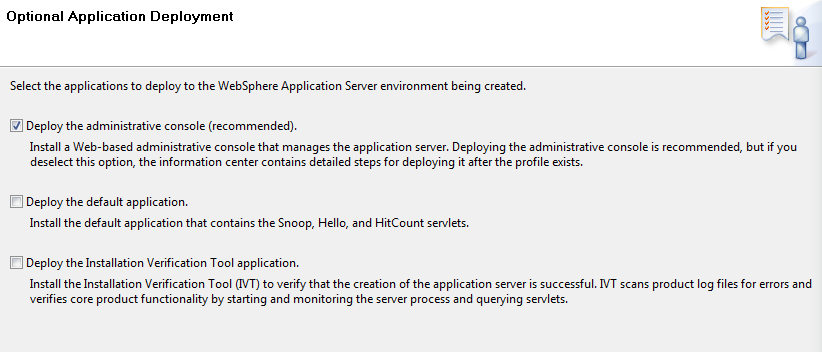
\includegraphics{./images-dxp/websphere-01-profile.png}
  \caption{Choose the Advanced profile option to specify your own
  settings.}
  \end{figure}
\item
  Check the box \emph{Deploy the administrative console}. This gives you
  a web-based UI for working with your application server. Skip the
  default applications. You'd only install these on a development
  machine. Click \emph{Next}.
\item
  Set the profile name and location. Ensure you specify a performance
  tuning setting other than \emph{Development}, since you're installing
  a production server. See the WebSphere documentation for more
  information about performance tuning settings. Click \emph{Next}.
\item
  Choose node, server, and host names for your server. These will be
  specific to your environment. Click \emph{Next}.
\item
  Administrative security in WebSphere is a way to restrict who has
  access to the administrative tools. You may want to have it enabled in
  your environment so that a user name and password are required to
  administer the WebSphere server. See WebSphere's documentation for
  more information. Click \emph{Next}.
\item
  Each profile needs a security certificate, which comes next in the
  wizard. If you don't have certificates already, choose the option to
  generate a personal certificate and a signing certificate and click
  \emph{Next}.
\item
  Once the certificates are generated, set a password for your keystore.
  Click \emph{Next}.
\item
  Now you can customize the ports this server profile uses. Be sure to
  choose ports that are open on your machine. When choosing ports, the
  wizard detects existing WebSphere installations and if it finds
  activity, it increments ports by one.
\item
  Choose whether you want this profile started when the machine starts.
  Click \emph{Next}.
\item
  WebSphere ships with IBM HTTP Server, which is a re-branded version of
  Apache. Choose whether you want a web server definition, so that this
  JVM receives requests forwarded from the HTTP server. See WebSphere's
  documentation for details on this. When finished, click \emph{Next}.
\item
  The wizard then shows you a summary of what you selected, enabling you
  to keep your choices or go back and change something. When you're
  satisfied, click \emph{Next}.
\end{enumerate}

WebSphere then creates your profile and finishes with a message telling
you the profile was created successfully. Awesome! Your profile is
complete. Now there are a few things you need to configure in your
application server.

\begin{figure}
\centering
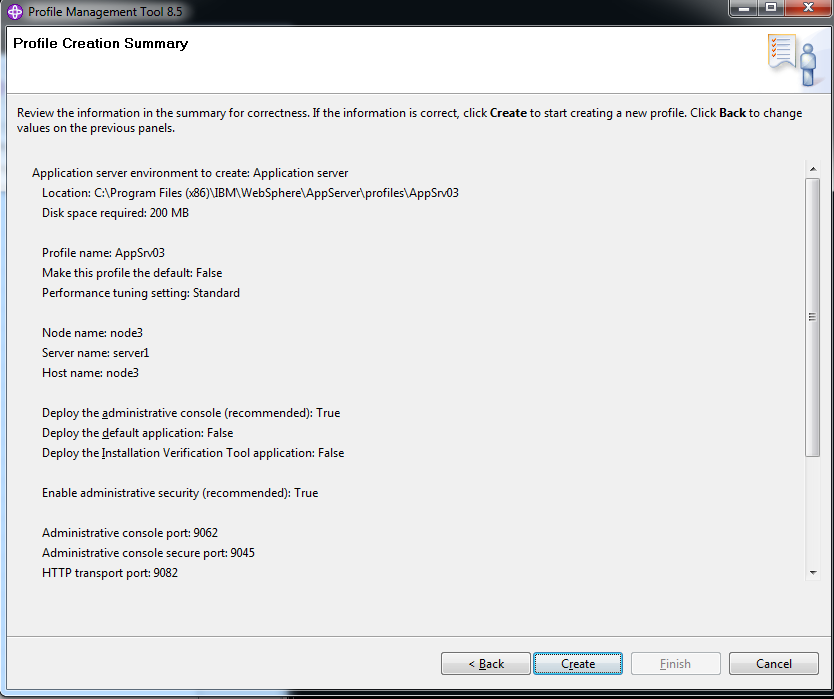
\includegraphics{./images-dxp/websphere-02-profile.png}
\caption{Example of the settings before creating the profile.}
\end{figure}

\subsection{Configuring the WebSphere Application
Server}\label{configuring-the-websphere-application-server}

In this version of WebSphere, servlet filters are not initialized on web
application startup, but rather, on first access. This can cause
problems when deploying certain apps to Liferay DXP. To configure
servlet filters to initialize on application startup (i.e., deployment),
you need to set the following \texttt{webcontainer} custom properties in
your WebSphere application server:

\begin{verbatim}
com.ibm.ws.webcontainer.initFilterBeforeInitServlet = true
com.ibm.ws.webcontainer.invokeFilterInitAtStartup = true
\end{verbatim}

To set \texttt{webcontainer} custom properties in the WebSphere
application server, follow the instructions
\href{http://www-01.ibm.com/support/docview.wss?rss=180&uid=swg21284395}{here
in WebSphere's documentation}.

\subsection{Setting up JVM Parameters for Liferay
DXP}\label{setting-up-jvm-parameters-for-liferay-dxp}

Next, in the WebSphere profile you created for Liferay DXP, you must set
an argument that supports Liferay DXP's Java memory requirements. You'll
modify this file:

\begin{verbatim}
[Install Location]/WebSphere/AppServer/profiles/your-profile/config/cells/your-cell/nodes/your-node/servers/your-server/server.xml
\end{verbatim}

Add \texttt{maximumHeapSize="2048"} inside the \texttt{jvmEntries} tag.
For example:

\begin{verbatim}
<jvmEntries xmi:id="JavaVirtualMachine_1183122130078" ... maximumHeapSize="2048">
\end{verbatim}

\noindent\hrulefill

\textbf{Note:} The JVM parameters used here are defaults intended for
production systems development purposes. Administrators can change the
settings to other values that best address their specific environments.
These will need to be tuned depending on need.

\noindent\hrulefill

Administrators can set the UTF-8 and GMT time zone properties in the
\texttt{server.xml} file. This is required or else special characters
will not be parsed correctly. Add the following inside the
\texttt{jvmEntries} tag:

\begin{verbatim}
<jvmEntries xmi:id="JavaVirtualMachine_1183122130078" ...genericJvmArguments="-Dfile.encoding=UTF-8 -Duser.timezone=GMT">
\end{verbatim}

\noindent\hrulefill

\textbf{Important:} For Liferay DXP to work properly, the application
server JVM must use the \texttt{GMT} time zone and \texttt{UTF-8} file
encoding.

\noindent\hrulefill

Alternately, you can set the UTF-8 and GMT properties from the WebSphere
Admin Console. (See below.)

\subsection{Removing the secureSessionCookie
Tag}\label{removing-the-securesessioncookie-tag}

In the same profile, you should delete a problematic
\texttt{secureSessionCookie} tag that can cause Liferay DXP startup
errors. Note that this is just a default setting; once Liferay DXP is
installed, you should tune it appropriately based on your usage.

In
\texttt{{[}Install\ Location{]}/WebSphere/AppServer/profiles/your-profile/config/cells/your-cell/cell.xml},
Delete the \texttt{secureSessionCookie} tag containing
\texttt{xmi:id="SecureSessionCookie\_1"}.

If this tag is not removed, an error similar to the one here may occur:

\begin{verbatim}
WSVR0501E: Error creating component com.ibm.ws.runtime.component.CompositionUnitMgrImpl@d74fa901    
com.ibm.ws.exception.RuntimeWarning: com.ibm.ws.webcontainer.exception.WebAppNotLoadedException: Failed to load webapp: Failed to load webapp: SRVE8111E: The application, LiferayEAR, is trying to modify a cookie which matches a pattern in the restricted programmatic session cookies list [domain=*, name=JSESSIONID, path=/].
\end{verbatim}

\subsection{Installing Liferay DXP's
Dependencies}\label{installing-liferay-dxps-dependencies}

You must now install Liferay DXP's dependencies. Recall that earlier you
downloaded two ZIP files containing these dependencies. Install their
contents now:

\begin{enumerate}
\def\labelenumi{\arabic{enumi}.}
\item
  \texttt{liferay-dxp-digital-enterprise-dependencies-{[}version{]}.zip}:
  Unzip this file and place its contents in your WebSphere application
  server's \texttt{{[}Install\ Location{]}/WebSphere/AppServer/lib/ext}
  folder. If you have a JDBC database driver \texttt{JAR}, copy it to
  this location as well.
\item
  \texttt{liferay-dxp-digital-enterprise-osgi-{[}version{]}.zip}: Unzip
  this file and place its contents in the
  \texttt{{[}Liferay\ Home{]}/osgi} folder (create this folder if it
  doesn't exist). This is typically
  \texttt{{[}Install\ Location{]}/WebSphere/AppServer/profiles/your-profile/liferay/osgi}.
\end{enumerate}

Before starting the server, verify that all the following jars have been
copied to the correct folders. Optional jars are available (italics) and
are used to optimize Liferay performance which must be added to this
folder. Required jars in bold are from the
\texttt{liferay-digital-enterprise-dependencies-7.0-ga1\ zip}. The
following files should be present within the \texttt{lib/ext} (WebSphere
Application) folder:

\begin{enumerate}
\def\labelenumi{\arabic{enumi}.}
\tightlist
\item
  \texttt{activation.jar}
\item
  \texttt{com.liferay.registry.api-1.0.4.jar}
\item
  \texttt{hsql.jar}
\item
  A JDBC database jar (e.g.~MySQL, MariaDB, IBM DB2, Postgres)
\item
  \texttt{persistence.jar}
\item
  \texttt{portal-kernel.jar}
\item
  \texttt{portlet.jar}
\end{enumerate}

The following folders should be present within the
\texttt{/liferay/osgi} folder:

\begin{enumerate}
\def\labelenumi{\arabic{enumi}.}
\tightlist
\item
  \texttt{Configs}
\item
  \texttt{Core}
\item
  \texttt{Marketplace}
\item
  \texttt{Target-platform}
\item
  \texttt{Test}
\end{enumerate}

Once you've installed these dependencies, start the server profile you
created for Liferay DXP. Once it starts, you're ready to configure your
database.

\subsection{Database Configuration}\label{database-configuration-4}

If you want WebSphere to manage the database connections, follow the
instructions below. Note this is not necessary if you're planning on
using Liferay DXP's standard database configuration; in that case, skip
this section. You'll set your database information in Liferay DXP's
setup wizard after the install.

\noindent\hrulefill

\textbf{Note:} Although Liferay DXP's embedded database is fine for
testing purposes, you \textbf{should not} use it for production Liferay
DXP instances.

\noindent\hrulefill

\begin{verbatim}
![ WebSphere JDBC providers](./images-dxp/websphere-jdbc-providers.png)
\end{verbatim}

\begin{enumerate}
\def\labelenumi{\arabic{enumi}.}
\item
  Start WebSphere.
\item
  Open the Administrative Console and log in.
\item
  Click \emph{Resources → JDBC Providers}.
\item
  Select a scope and then click \emph{New}.
\item
  Select your database type, provider type, and implementation type. If
  you select a predefined database, the wizard fills in the name and
  description fields for you. If the database you want to use isn't
  listed, select \emph{User-defined} from the \emph{Database type} field
  and then fill in the \emph{Implementation Class Name}. For example, if
  you are using MySQL, select \emph{Database type} →
  \emph{User-defined}, and then enter
  \texttt{com.mysql.jdbc.jdbc2.optional.MysqlConnectionPoolDataSource}
  in \emph{Implementation Class Name}. Click \emph{Next} when you are
  finished.
\item
  Clear any text in the classpath settings. You already copied the
  necessary JARs to a location on the server's classpath. Click
  \emph{Next}.
\item
  Review your settings and click \emph{Finish}. The final configuration
  should look like this:

  \begin{figure}
  \centering
  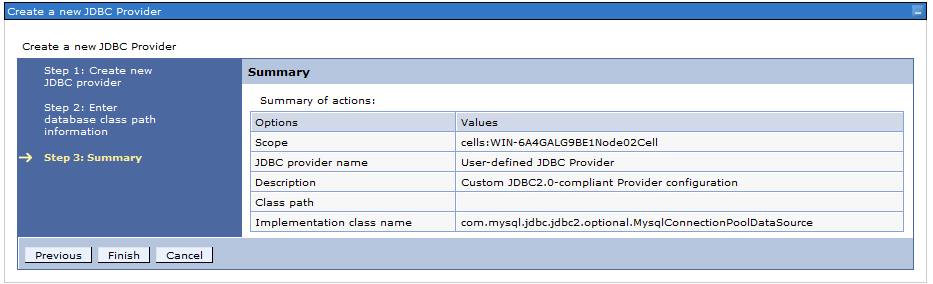
\includegraphics{./images-dxp/websphere-03.png}
  \caption{Completed JDBC provider configurations.}
  \end{figure}
\item
  Click your new provider configuration when it appears in the table,
  and then click \emph{Data Sources} under \emph{Additional Properties}.
  Click \emph{New}.
\item
  Enter \emph{liferaydatabasesource} in the \emph{Data source name}
  field and \texttt{jdbc/LiferayPool} in the \emph{JNDI name} field.
  Click \emph{Next}.
\item
  Click \emph{Next} in the remaining screens of the wizard to accept the
  default values. Then review your changes and click \emph{Finish}.
\item
  Click the data source when it appears in the table and then click
  \emph{Custom Properties}. Now click the \emph{Show Filter Function}
  button. This is the second from last of the small icons under the
  \emph{New} and \emph{Delete} buttons.
\item
  Type \emph{user} into the search terms and click \emph{Go}.

  \begin{figure}
  \centering
  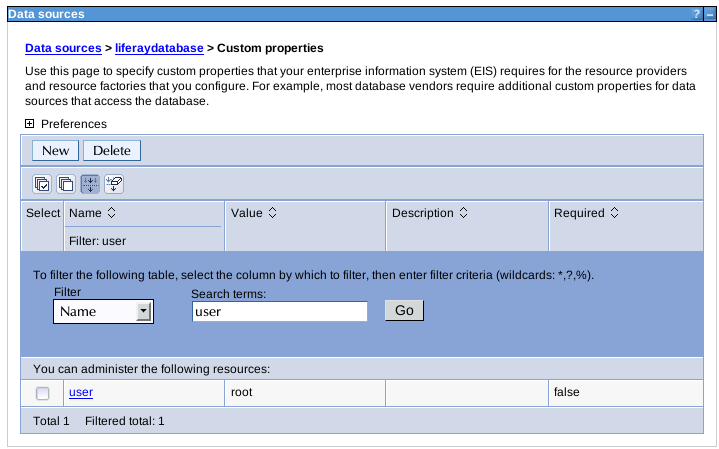
\includegraphics{./images-dxp/websphere-database-properties.png}
  \caption{Modifying data source properties in WebSphere}
  \end{figure}
\item
  Select the \emph{user} property and give it the value of the user name
  to your database. Click \emph{OK} and save to master configuration.
\item
  Do another filter search for the \emph{url} property. Give this
  property a value that points to your database. For example, a MySQL
  URL would look like this:

\begin{verbatim}
jdbc:mysql://localhost/lportal?useUnicode=true&characterEncoding=UTF-8&useFastDateParsing=false
\end{verbatim}

  Click \emph{OK} and save to master configuration.
\item
  Do another filter search for the \emph{password} property. Enter the
  password for the user ID you added earlier as the value for this
  property. Click \emph{OK} and save to master configuration.
\item
  Go back to the data source page by clicking it in the breadcrumb
  trail. Click the \emph{Test Connection} button. It should connect
  successfully.
\end{enumerate}

Once you've set up your database, you can set up your mail session.

\subsection{Mail Configuration}\label{mail-configuration-4}

If you want WebSphere to manage your mail sessions, use the following
procedure. If you want to use Liferay DXP's built-in mail sessions, you
can skip this section.

\subsection{Creating a WebSphere-Managed Mail Session
(Optional)}\label{creating-a-websphere-managed-mail-session-optional}

\begin{enumerate}
\def\labelenumi{\arabic{enumi}.}
\item
  Click \emph{Resources → Mail → Mail Providers}.
\item
  Click the Built-In Mail Provider for your node and server.
\item
  Click \emph{Mail Sessions} and then click the \emph{New} button.
\item
  Give your mail session a name of \emph{liferaymail} and a JNDI name of
  \texttt{mail/MailSession}. Fill in the correct information for your
  mail server in the sections \emph{Outgoing Mail Properties} and
  \emph{Incoming Mail Properties}. Click \emph{OK} and then save to the
  master configuration.
\item
  Click your mail session when it appears in the table and select
  \emph{Custom Properties} under the \emph{Additional Properties}
  section. Set any other JavaMail properties required by your mail
  server, such as the protocol, ports, whether to use SSL, and so on.
\item
  Click \emph{Security → Global Security} and de-select \emph{Use Java 2
  security to restrict application access to local resources} if it is
  selected. Click \emph{Apply}.
\end{enumerate}

Note that you may also need to retrieve a SSL certificate from your mail
server and add it to WebSphere's trust store. See WebSphere's
documentation for instructions on this.

\subsection{Verifying WebSphere Mail
Provider}\label{verifying-websphere-mail-provider}

To validate that the mail session has been configured correctly, there
are a number of ways to test this once the WAR has been deployed, the
server has started, and the user has signed in as the system
administrator. One quick way to validate is to create a new user with a
valid email account. The newly created user should receive an email
notification. The logs should display that the SMTP server has been
pinged with the correct port number listed.

\subsection{Enable Cookies for HTTP
Sessions}\label{enable-cookies-for-http-sessions}

WebSphere 8.5.5.9 restricts cookies to HTTPS sessions by default. If
you're using HTTP instead, this prevents users from signing in to
Liferay DXP and displays the following error in the console:

\begin{verbatim}
20:07:14,021 WARN  [WebContainer : 1][SecurityPortletContainerWrapper:341]
User 0 is not allowed to access URL http://localhost:9081/web/guest/home and
portlet com_liferay_login_web_portlet_LoginPortlet
\end{verbatim}

This occurs because Liferay DXP can't use the HTTPS cookie when you use
HTTP. The end result is that new sessions are created on each page
refresh. Follow these steps to resolve this issue in WebSphere:

\begin{enumerate}
\def\labelenumi{\arabic{enumi}.}
\item
  Click \emph{Application Servers} → \emph{server1} → \emph{Session
  Management} → Enable Cookies
\item
  De-select \emph{Restrict cookies to HTTPS sessions}
\item
  Click \emph{Apply}
\item
  Click \emph{Save}
\end{enumerate}

\subsection{Enable UTF-8}\label{enable-utf-8}

If you did not add the \texttt{-Dfile.encoding=UTF-8} property in the
\texttt{server.xml}, you can do so in the Administrative Console.

\begin{enumerate}
\def\labelenumi{\arabic{enumi}.}
\item
  Click \emph{Application Servers} → \emph{server1} → \emph{Process
  definition}.
\item
  Click \emph{Java Virtual Machine} under \emph{Additional Properties}.
\item
  Enter \texttt{-Dfile.encoding=UTF-8} in the \emph{Generic JVM
  arguments} field.
\item
  Click \emph{Apply} and then \emph{Save} to master configuration.
\end{enumerate}

Once the changes have been saved, Liferay DXP can parse special
characters if there is localized content.

\subsection{Deploy Liferay DXP}\label{deploy-liferay-dxp-2}

Now you're ready to deploy Liferay DXP!

\begin{enumerate}
\def\labelenumi{\arabic{enumi}.}
\item
  In WebSphere's administrative console, click \emph{Applications} →
  \emph{New Application} → \emph{New Enterprise Application}.
\item
  Browse to the Liferay DXP \texttt{.war} file, select it, and click
  \emph{Next}.
\item
  Leave \emph{Fast Path} selected and click \emph{Next}. Ensure that
  \emph{Distribute Application} has been checked and click \emph{Next}
  again.
\item
  Choose the WebSphere runtimes and/or clusters where you want Liferay
  DXP deployed. Click \emph{Next}.
\item
  Select the virtual host to deploy Liferay DXP on and click
  \emph{Next}.
\item
  Map Liferay DXP to the root context (/) and click \emph{Next}.
\item
  Select the \emph{metadata-complete attribute} setting that you want to
  use and click \emph{Next}.
\item
  Ensure that you have made all the correct choices and click
  \emph{Finish}. When Liferay DXP has installed, click \emph{Save to
  Master Configuration}.

  \begin{figure}
  \centering
  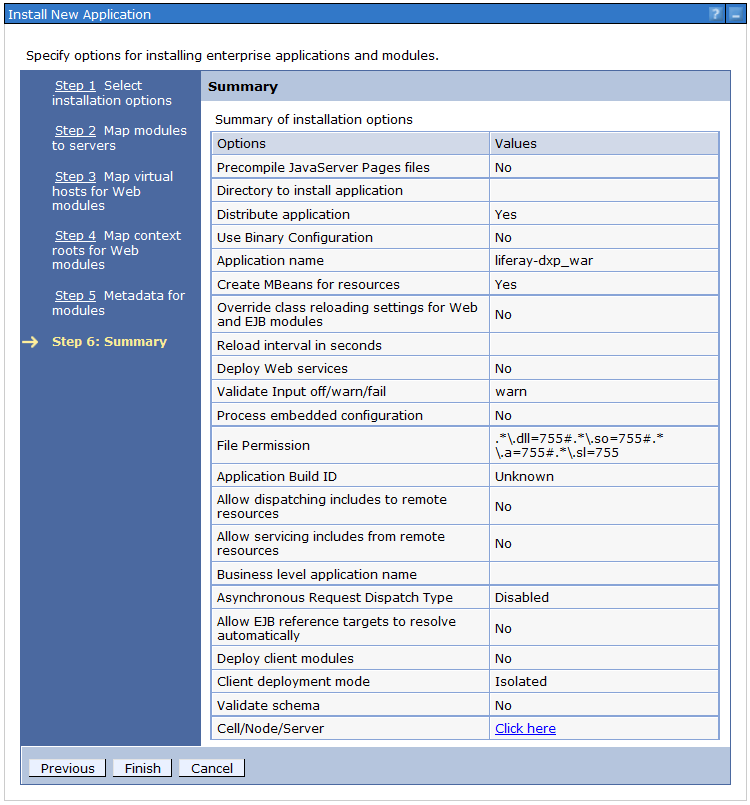
\includegraphics{./images-dxp/websphere-deploy-dxp.png}
  \caption{Review your deployment options before deploying.}
  \end{figure}
\end{enumerate}

You've now installed Liferay DXP!

\subsection{Setting the JDK Version for Compiling
JSPs}\label{setting-the-jdk-version-for-compiling-jsps}

Liferay DXP requires that its JSPs are compiled on Java 8. To ensure
that WebSphere does this, shut down WebSphere after you've deployed the
Liferay DXP \texttt{.war} file. Navigate to the \texttt{WEB\_INF} folder
and add the following setting to the \texttt{ibm-web-ext.xml} or in most
cases the \texttt{ibm-web-ext.xmi} file:

\begin{verbatim}
<jsp-attribute name="jdkSourceLevel" value="18" />
\end{verbatim}

The exact path to the \texttt{ibm-web-ext.xmi} file depends on your
WebSphere installation location and Liferay DXP version, but here's an
example:

\begin{verbatim}
/opt/IBM/WebSphere/AppServer/profiles/AppSrv01/config/cells/localhostNode01Cell/applications/liferayXX.ear/deployments/liferayXX/liferayXX.war/WEB-INF/ibm-web-ext.xmi
\end{verbatim}

Note that the Liferay DXP \texttt{.war} comes pre-packaged with the
\texttt{ibm-web-ext.xmi} file; this format is functionally the same as
\texttt{.xml} and WebSphere recognizes both formats. For more general
information on how WebSphere compiles JSPs see IBM's official
documentation for
\href{https://www.ibm.com/support/knowledgecenter/en/SSAW57_8.5.5/com.ibm.websphere.nd.doc/ae/rweb_jspengine.html}{WebSphere
Application Server 8.5.5.x}.

Now restart WebSphere.

\subsection{Enabling Security for Portal Access Control
Lists}\label{enabling-security-for-portal-access-control-lists}

When you are ready to start using apps from Liferay Marketplace, you
must enable Liferay's Portal Access Control Lists (PACL) to enforce
security policies on Marketplace applications. To do so, you must enable
Java Security on your WebSphere server and specify a security policy to
grant Liferay DXP access to your server.

In WebSphere's administrative console, go to \emph{Security} →
\emph{Global Security}. Check the box to enable Java 2 security, and
click \emph{Apply}. Save to the master configuration.

Now you must configure the security policy for the IBM JRE that
WebSphere runs on. With your WebSphere server shut down, open the
following security policy file:

\begin{verbatim}
[WebSphere-Install-Location]/java_1.8_64/jre/lib/security/java.policy
\end{verbatim}

Replace this file's contents with the following configuration:

\begin{verbatim}
grant {
    permission java.security.AllPermission;
};
\end{verbatim}

This configuration opens all permissions. As best practices, opening all
permissions when starting Liferay Digital Enterprise 7.0 for the first
time allows for the creation of all required processes. Users can change
security settings later and restrict which plugins have access. (Users
have the options of using either the application server's security
policies or Liferay DXP's.) See this article
\href{https://customer.liferay.com/documentation/knowledge-base/-/kb/156397}{concerning
a Known Issues when generating PACL}.

Once this permission has been set, users can start Liferay DXP.

\subsection{Start Liferay DXP}\label{start-liferay-dxp}

\begin{enumerate}
\def\labelenumi{\arabic{enumi}.}
\item
  If you plan to use Liferay DXP's setup wizard, skip to the next step.
  If you wish to use WebSphere's data source and mail session, create a
  file called \texttt{portal-ext.properties} in your Liferay Home
  folder. Place the following configuration in the file:

\begin{verbatim}
 jdbc.default.jndi.name=jdbc/LiferayPool
 mail.session.jndi.name=mail/MailSession
 setup.wizard.enabled=false
\end{verbatim}
\item
  In the WebSphere administrative console, navigate to \emph{Enterprise
  Applications}, select the Liferay DXP application, and click
  \emph{Start}. While Liferay DXP is starting, WebSphere displays a
  spinny little graphic. Don't watch it too closely, or you might get
  hypnotized.
\item
  In Liferay DXP's setup wizard, select and configure your database
  type. Click \emph{Finish} when you're done. Liferay DXP then creates
  the tables it needs in the database.
\end{enumerate}

Congratulations! You've installed Liferay DXP on WebSphere!

\section{Installing Elasticsearch}\label{installing-elasticsearch}

Liferay DXP uses Elasticsearch to index its content. By default,
Liferay DXP uses Elasticsearch as an embedded service. It works, but this
is not a supported configuration for a production server. Feel free to
use it while you're testing or developing, but when you're ready to put
your site in production, you'll need to run Elasticsearch as a
standalone process. This is better anyway, because it frees you to
design your infrastructure the way you want it. If you've got hardware
or a VM to spare, you can separate your search infrastructure from
Liferay DXP and reap some performance gains by putting search on a
separate box. If you're more budget-conscious, you can still increase
performance by running Elasticsearch in a separate, individually tunable
JVM on the same box.

Installing Elasticsearch for Liferay DXP is pretty easy and takes only
six steps:

\begin{enumerate}
\def\labelenumi{\arabic{enumi}.}
\item
  Find the version of Elasticsearch that's embedded in the version of
  Liferay DXP you have, and then download that version from
  \href{https://www.elastic.co}{Elastic's} website.
\item
  Install Elasticsearch by extracting its archive to the system where
  you want it to run.
\item
  Install some required Elasticsearch plugins.
\item
  Name your Elasticsearch cluster.
\item
  Configure Liferay DXP to connect to your Elasticsearch cluster.
\item
  Restart Liferay DXP and reindex your search and spell check indexes.
\end{enumerate}

\noindent\hrulefill

\textbf{Note:} Before continuing, make sure you have set the
\href{https://docs.oracle.com/cd/E19182-01/820-7851/inst_cli_jdk_javahome_t/}{\texttt{JAVA\_HOME}
environment variable}

If you have multiple JDKs installed, make sure Elasticsearch and Liferay
DXP are using the same version. You can specify this in
\texttt{{[}Elasticsearch\ \ Home{]}/bin/elasticsearch.in.sh}:

\begin{verbatim}
     JAVA_HOME=/path/to/java
\end{verbatim}

\noindent\hrulefill

Now you'll actually perform these steps, and when you're done, you'll
have a production-ready instance of Liferay DXP up and running. After
you're done following the installation guide, refer to the
\href{/docs/7-0/deploy/-/knowledge_base/d/configuring-elasticsearch-for-liferay-0}{Configuring
Elasticsearch} article for more details on configuring Liferay DXP for
Elasticsearch. For more information on installing a search engine, see
\href{/docs/7-0/deploy/-/knowledge_base/d/installing-a-search-engine}{here}.

\subsection{Step One: Find the Right Version of
Elasticsearch}\label{step-one-find-the-right-version-of-elasticsearch}

If Liferay DXP isn't running, start it.

Visit port 9200 on localhost to access the embedded Elasticsearch:

\begin{verbatim}
http://localhost:9200
\end{verbatim}

A JSON document is returned that varies slightly, but should look
similar to this:

\begin{verbatim}
{
  "name" : "Wiz Kid",
  "cluster_name" : "LiferayElasticsearchCluster",
  "version" : {
    "number" : "2.4.0",
    "build_hash" : "8ff36d139e16f8720f2947ef62c8167a888992fe",
    "build_timestamp" : "2016-08-27T13:32:39Z",
    "build_snapshot" : false,
    "lucene_version" : "5.5.2"
  },
  "tagline" : "You Know, for Search"
}
\end{verbatim}

The version of Elasticsearch that's running is the value of the
\texttt{"number"} field. In this example, it's \texttt{2.4.0}.

\noindent\hrulefill

\textbf{Elasticsearch 6:} Elasticsearch 6 is supported for Liferay
Digital Enterprise systems running Fix Pack 79 or later: see the
\href{https://www.liferay.com/documents/10182/246659966/Liferay+DXP+7.0+Compatibility+Matrix.pdf}{compatibility
matrix} for the exact version ranges supported for your Fix Pack level.
The latest Liferay Portal, GA 7 at the time of this writing, does not
support Elasticsearch 6.5. Instead use Elasticsearch 6.1. In 7.0,
Elasticsearch version 2.x remains the default, embedded version. To
install Elasticsearch 6.5.x,

\begin{enumerate}
\def\labelenumi{\arabic{enumi}.}
\item
  Make sure you're running at least Digital Enterprise FP-79.
\item
  Install Elasticsearch 6.5.x (follow steps 2-4 in this article for
  guidance).
\item
  Install the \href{https://web.liferay.com/marketplace}{\emph{Liferay
  Connector to Elasticsearch 6}, version 1.1.0+, from Marketplace} and
  stop the default Elasticsearch adapter.
\item
  Configure the Elasticsearch 6 connector (see step 5 below for
  guidance).
\end{enumerate}

To learn more about upgrading an existing system to Elasticsearch 6.5,
read the
\href{/docs/7-0/deploy/-/knowledge_base/d/upgrading-to-elasticsearch-6}{upgrade
article}.

\noindent\hrulefill

Now that you know the version of Elasticsearch you need, go to
\href{https://www.elastic.co}{Elastic's} website and download that
version.

\subsection{Step Two: Install
Elasticsearch}\label{step-two-install-elasticsearch}

Most of this step entails deciding where you want to run Elasticsearch.
Do you want to run it on the same machine as Liferay DXP, or do you want
to run it on its own hardware? The answer to this question comes down to
a combination of the resources you have available and the size of your
installation. Regardless of what you decide, either way you get the
benefit of a separately tunable search infrastructure.

Once you have a copy of the right version of Elasticsearch, extract it
to a folder on the machine where you want it running. That's all there
is to this step.

\subsection{Step Three: Install Elasticsearch
Plugins}\label{step-three-install-elasticsearch-plugins}

Install the following required Elasticsearch plugins:

\begin{itemize}
\tightlist
\item
  \texttt{analysis-icu}
\item
  \texttt{analysis-kuromoji}
\item
  \texttt{analysis-smartcn}
\item
  \texttt{analysis-stempel}
\end{itemize}

To install these plugins, navigate to Elasticsearch Home and enter

\begin{verbatim}
./bin/plugin install [plugin-name]
\end{verbatim}

Replace \emph{{[}plugin-name{]}} with the Elasticsearch plugin's name.

\noindent\hrulefill

\textbf{Elasticsearch 6.5:} The \texttt{plugin} executable was renamed
in Elasticsearch 6, to \texttt{elasticsearch-plugin}. The general
command syntax for installing plugins to 6.5 is

\begin{verbatim}
 ./bin/elasticsearch-plugin install [plugin-name]
\end{verbatim}

\noindent\hrulefill

\subsection{Step Four: Name Your Elasticsearch
Cluster}\label{step-four-name-your-elasticsearch-cluster}

A \emph{cluster} in Elasticsearch is a collection of nodes (servers)
identified as a cluster by a shared cluster name. The nodes work
together to share data and workload. A one node cluster is discussed
here; to create a multi-node cluster, please refer to
\href{https://www.elastic.co/guide/index.html}{Elastic's documentation}.

Now that you've installed Elastic, it sits in a folder on your machine,
which is referred to here as \texttt{{[}Elasticsearch\ Home{]}}. To name
your cluster, you'll define the cluster name in both Elasticsearch and
in Liferay DXP. First, define it in Elasticsearch. Edit the following
file:

\begin{verbatim}
[Elasticsearch Home]/config/elasticsearch.yml
\end{verbatim}

Uncomment the line that begins with \texttt{cluster.name}. Set the
cluster name to whatever you want to name your cluster:

\begin{verbatim}
cluster.name: LiferayElasticsearchCluster
\end{verbatim}

Of course, this isn't a very imaginative name; you may choose to name
your cluster \texttt{finders\_keepers} or something else you can
remember more easily. Save the file.

Now you can start Elasticsearch. Run the executable for your operating
system from the \texttt{{[}Elasticsearch\ Home{]}/bin} folder:

\begin{verbatim}
./elasticsearch
\end{verbatim}

Elasticsearch starts, and one of its status messages includes a
transport address:

\begin{verbatim}
2016-05-03 16:33:28,358][INFO ][transport] [Hobgoblin II] publish_address {127.0.0.1:9300}, bound_addresses {[::1]:9300}, {127.0.0.1:9300}
\end{verbatim}

Take note of this address; you'll need to give it to your Liferay DXP
server so it can find Elasticsearch on the network.

\subsection{Step Five: Configure Liferay DXP to Connect to your
Elasticsearch
Cluster}\label{step-five-configure-liferay-dxp-to-connect-to-your-elasticsearch-cluster}

\noindent\hrulefill

\textbf{Elasticsearch 6.5:} Before continuing, install the
\href{https://web.liferay.com/marketplace}{Liferay Connector to
Elasticsearch 6 application} from Liferay Marketplace and stop the
default Elasticsearch 2.x adapter, which connects to Elasticsearch 2.x.

\begin{enumerate}
\def\labelenumi{\arabic{enumi}.}
\item
  Create a file called

\begin{verbatim}
com.liferay.portal.bundle.blacklist.internal.BundleBlacklistConfiguration.config
\end{verbatim}

  If you already have one of these files in
  \texttt{Liferay\ Home/osgi/configs}, just open it.
\item
  Place the Bundle Symbolic Name of the Elasticsearch connector in the
  \texttt{blacklistBundleSymbolicNames} property:

\begin{verbatim}
 blacklistBundleSymbolicNames=["com.liferay.portal.search.elasticsearch"]
\end{verbatim}
\item
  Place the file in \texttt{Liferay\ Home/osgi/configs}.
\end{enumerate}

Alternatively, deactivate the Elasticsearch connector using the App
Manager in \emph{Control Panel} → \emph{Apps} → \emph{App Manager}. If
you're a Digital Enterprise customer, use the blacklist feature as
described above. The App Manager relies on the \texttt{osgi/state}
folder to ``remember'' the state of the bundle. If you delete this
folder (recommended during patching) the Elasticsearch connector will be
reinstalled and started automatically.

\begin{enumerate}
\def\labelenumi{\arabic{enumi}.}
\item
  Search for \emph{elasticsearch} in the App Manager. Find the Liferay
  Portal Search Elasticsearch module and click the edit
  ((\includegraphics{./images/icon-edit.png})) button. Choose the
  Deactivate option. This leaves the bundle installed, but stops it in
  the OSGi runtime.
\item
  Once you've downloaded the LPKG file with the Elasticsearch 6 adapter,
  place it in Liferay Home's \texttt{deploy} folder. Find more detailed
  information on deploying Marketplace applications
  \href{/docs/7-0/user/-/knowledge_base/u/using-the-liferay-marketplace}{here}.
\end{enumerate}

\noindent\hrulefill

Now you're ready to configure Liferay DXP. Start Liferay DXP if you
haven't already, log in, and then click on \emph{Control Panel} →
\emph{Configuration} → \emph{System Settings} → \emph{Foundation}. Find
\emph{Elasticsearch} (or \emph{Elasticsearch 6})in the list of settings
and click on it. Now you can configure it. Here are the options you need
to change:

\textbf{Cluster name:} Enter the name of the cluster as you defined it
in Elasticsearch.

\textbf{Operation mode:} Defaults to EMBEDDED. Change it to REMOTE to
connect to a standalone Elasticsearch.

\textbf{Transport addresses:} Enter a delimited list of transport
addresses for Elasticsearch nodes. Here, you'll enter the transport
address from the Elasticsearch server you started. The default value is
\texttt{localhost:9300}, which will work.

When finished, click \emph{Save}. You're almost done.

\subsection{Step Six: Restart Liferay DXP and
Reindex}\label{step-six-restart-liferay-dxp-and-reindex}

Stop and restart Liferay DXP. When it's back up, log in as an
administrative user and

\begin{enumerate}
\def\labelenumi{\arabic{enumi}.}
\item
  Click on \emph{Control Panel} → \emph{Configuration} → \emph{Server
  Administration}
\item
  Click the \emph{Execute} button for \emph{Reindex all search indexes}.
  When you do that, you should see some messages scroll up in the
  Elasticsearch log.
\item
  Click Execute for \emph{Reindex all spell check indexes}.
\end{enumerate}

For more details refer to the
\href{https://www.elastic.co/guide/en/elasticsearch/reference/2.4/_installation.html}{Elasticsearch
installation guide}.

You're almost done! The only thing left is to make sure Marketplace is
working and optionally configure portal security.

\section{Liferay DXP Trial Plugin
Installation}\label{liferay-dxp-trial-plugin-installation}

For Liferay customers who are evaluating Liferay DXP on a trial basis,
\textbf{the plugins can be accessed from within the Marketplace section
of the Control Panel in the product}.

\emph{At a later date, the Marketplace website on Liferay.COM will be
accessible to Liferay DXP Trial customers. For now, please access EE
Plugins through the portal installation itself.}

\subsection{The Installation Process}\label{the-installation-process}

\textbf{1)} Sign into your Liferay.COM account (LRDC) on the home page.
If you don't have an account, please register by clicking the same link.

\begin{figure}
\centering
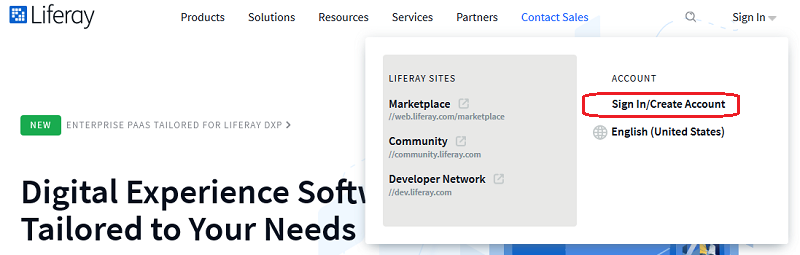
\includegraphics{./images-dxp/liferay-com-sign-in.png}
\caption{Click the hamburger menu to sign in or create an account.}
\end{figure}

\textbf{2)}You must be running Liferay DXP (Trial License is OK).

\textbf{3)} After signing in as an Admin in your Liferay DXP Trial
server, go to the Control Panel and configure the Liferay.COM (LRDC)
account to login to the Marketplace (click ``Store''). Authorize
Marketplace to access your local account.

\begin{figure}
\centering
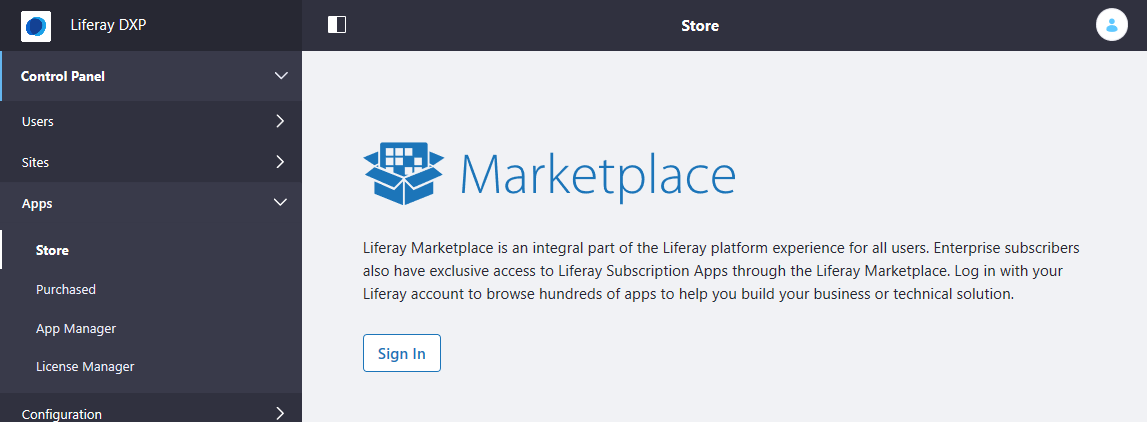
\includegraphics{./images-dxp/dxp-store-link.png}
\caption{Click the \emph{Store} link and authorize Marketplace to access
your local account.}
\end{figure}

\textbf{4)} \textbf{Important}: Once signed into the Store, click on the
\emph{Purchased} link, and then click on the \emph{EE} subtab.

\begin{figure}
\centering
\includegraphics{./images-dxp/dxp-store-ee.png}
\caption{The trial plugins are available as plugins already purchased.}
\end{figure}

Here you can see a list of Liferay DXP plugins that are installed, as
well as options to update or install certain plugins. To install a
plugin, click the \emph{Install} button located to the far right of the
respective plugin.

\begin{figure}
\centering
\includegraphics{./images-dxp/dxp-store-install.png}
\caption{Click the \emph{Install} button to install a plugin.}
\end{figure}

\textbf{5)} Trial users have access to the Customer Portal during their
trial. This also includes access to the Liferay DXP-specific plugins
from the Liferay \href{https://www.liferay.com/marketplace}{Marketplace
website} on Liferay.COM (LRDC). Trial users do not have access to our
customer Knowledge Base and \href{https://help.liferay.com/hc}{Help
Center} (our support ticketing system).

\noindent\hrulefill

Note: We are currently working on providing access to Liferay DXP
Plugins on the Marketplace website for Liferay DXP Trial customers,
which would also include access from within the portal installation.

\noindent\hrulefill

\subsection{FAQ}\label{faq}

\textbf{Q:} Where are the ``Liferay DXP Trial Plugins''?

\textbf{A:} There is no such thing. The Liferay DXP Plugins in Liferay
Marketplace are the same ones that you get to try out with your Liferay
DXP Trial license for your portal. The Liferay DXP license (Trial or
official Liferay DXP Subscriber) gives you access to the Liferay DXP
plugins. (Also, there is no difference code-wise or release-wise between
a Liferay DXP Trial installation and a regular Liferay DXP non-Trial
installation. The only difference is the license.)

\textbf{Q:} Why can't I go to liferay.com/marketplace? Why can't I
``purchase'' from the Marketplace site?

\textbf{A:} DXP Trial users must use the Marketplace accessed from
within the product's Control Panel (instructions above). You do not need
to ``purchase'' any DXP plugins because if you access Marketplace from
within the Control Panel, Marketplace sees that you have an DXP license
installed and gives access to DXP plugins. Official DXP Subscription
customers (i.e., non Trial) will be able to log into liferay.com with
their designated DXP subscriber login and access all DXP plugins through
the Marketplace website.

\textbf{Q:} Why are the plugins under the ``Purchased'' tab? If I click
on the ``DXP Marketplace'' link, it does not allow me to get the DXP
plugins.

\textbf{A:} Once you're signed into the Store, click on the
\emph{Purchased} tab, then click on the \emph{EE} subtab.

\textbf{Q:} What happens when DXP Trial customers become official
Liferay Digital Experience subscribers?

\textbf{A:} They will still be able to complete the above process, or
they can also visit the
\href{https://www.liferay.com/marketplace}{Liferay Marketplace website}.

\textbf{Q:} Do DXP Trial customers get the DXP source code?

\textbf{A:} No, they can only install the plugin. The DXP source code
becomes available once they are official Liferay DXP Enterprise
subscribers.

\textbf{Q:} Can this process of installing DXP plugins be used from
Liferay Portal CE (Community Edition)?

\textbf{A:} No, the Marketplace must detect that you are running Liferay
DXP.

\section{Activating Liferay DXP}\label{activating-liferay-dxp}

There are 2 ways to activate your Liferay DXP instance:

\begin{itemize}
\item
  With an XML activation key that you request and receive from Liferay
  Support.
\item
  Online activation through Liferay Connected Services (LCS). Liferay
  DXP 7.0 introduced LCS as a way to activate Liferay DXP instances. LCS
  can also install fix packs, monitor each instance's performance, and
  help administrators automatically manage Liferay DXP subscriptions.
  See the
  \href{/docs/7-0/deploy/-/knowledge_base/d/managing-liferay-with-liferay-connected-services}{LCS
  documentation} for instructions on activating your instances with LCS.
\end{itemize}

\noindent\hrulefill

\textbf{Note:} You must use LCS for activation of containerized
instances, cloud deployments, and instances that use Liferay Analytics
Cloud and/or elastic subscriptions. Otherwise, you don't have to use LCS
for activation. You can instead request an XML activation key from
Liferay Support.

\section{Setting Up Marketplace and Portal
Security}\label{setting-up-marketplace-and-portal-security}

Liferay Marketplace is more than just a store for Liferay applications.
Under the hood, it not only provides the store, it also provides Liferay
DXP's application deployment features. For this reason, you must ensure
that Marketplace works well on your installed system. The first thing
you should do is make sure Marketplace can run and configure itself. The
second thing you should do is enable Liferay's Portal Access Control
List, or PACL.

First, you'll learn about some scenarios in which Marketplace fails to
run, but they can all be worked around. Next, you'll configure PACL.

\subsection{Server is Firewalled without Access to the
Internet}\label{server-is-firewalled-without-access-to-the-internet}

Your server might be behind a firewall that prevents access to the
Internet. Or your security policy might not allow direct download and
installation from the Internet. In these cases, you have two options:

\begin{enumerate}
\def\labelenumi{\arabic{enumi}.}
\item
  From an Internet-enabled computer, download the Marketplace plugin
  from \url{https://www.liferay.com/marketplace/download}. Then allow
  Liferay DXP to auto deploy it by dropping the downloaded
  \texttt{.lpkg} file into the Liferay DXP deploy folder.
\item
  Alternately, once you have the downloaded \texttt{.lpkg} file, use the
  Liferay App Manager to deploy the plugin. This option is especially
  helpful if the application server does not support hot deploy. See
  \href{/docs/7-0/user/-/knowledge_base/u/installing-apps-manually}{Installing
  Apps Manually}.
\end{enumerate}

\subsection{Application Server Does Not Support Hot
Deploy}\label{application-server-does-not-support-hot-deploy}

If your application server does not support hot deploy, you can't
leverage Liferay DXP's auto deploy feature. You can, however, manually
deploy the plugin in two steps:

\begin{enumerate}
\def\labelenumi{\arabic{enumi}.}
\item
  Use Liferay DXP's tools to pre-deploy the file.
\item
  Then use your app server's tools to do the actual deployment.
\end{enumerate}

\subsection{Limited Database Access}\label{limited-database-access}

Some production environments do not have the necessary database
permissions for Liferay DXP and its plugins to maintain their tables. In
these cases:

\begin{enumerate}
\def\labelenumi{\arabic{enumi}.}
\item
  Grant the Liferay DXP database user temporary full rights to the
  database.
\item
  Install Liferay DXP and start it so that it populates its database.
\item
  Once the database is created, remove the permissions for creating
  tables and dropping tables from the Liferay DXP database user.
\end{enumerate}

See the Setting Up Liferay DXP's Database with Restrictive Permissions
section above for more information. Note that many sophisticated Liferay
DXP apps--not just the Marketplace plugin--require new tables when
deployed. If your environment restricts database access, you may need to
repeat the above steps whenever you deploy a new app to the Liferay DXP.

\subsection{Configuring Liferay DXP
Security}\label{configuring-liferay-dxp-security}

Liferay Marketplace is an online store for obtaining applications that
run on the Liferay DXP platform. These applications are provided not
only by Liferay DXP, but also by partners and independent developers who
want you to install and use their applications on your server. Many of
these applications are excellent and we recommend that you try them out
for yourself.

However, because many of the applications on Marketplace are \emph{not}
provided by Liferay DXP, a question arises: how do you know these
applications are doing what they're advertised to do? There is a vetting
process that they go through before they're allowed on Marketplace, but
if the source code is not provided, there's no way for even Liferay DXP
to know if an app has been properly represented. For this reason,
Liferay DXP implements a security feature known as the Portal Access
Control List, or PACL.

PACL forces an application to declare up front the functions from
Liferay DXP's APIs that it calls. Anything that's not declared is not
allowed to run. It's similar to what you might see on your mobile phone
when you install an app: you get to see the Liferay DXP API functions
the app uses, and then you can decide if you want to install that app
based on the permissions it requires. This way, you see right away what
portal data that app can access and the app can do nothing else: you're
protected--if you have PACL enabled. So if you plan to use apps
downloaded from Marketplace, it's important to make sure PACL is
enabled.

By default, Liferay DXP's bundles have PACL turned off. The reason for
this is that there is a small performance penalty for having PACL
enabled. Since the only reason to have PACL enabled is to install
untrusted third party apps from Marketplace (and not everybody does
that), we decided to leave PACL turned off by default. This way, your
portal performs as fast as possible.

The bottom is line that if you intend to use Marketplace apps, you
should enable PACL. We provide manually installation documentation for
all the app servers supported by Liferay DXP. Each of those sections has
a section that explains how to enable Java security for that app
server, which is a prerequisite for enabling PACL. Once you have Java
security enabled, PACL can be enabled by adding one line to your
\texttt{portal-ext.properties} or
\texttt{portal-setup-wizard.properties} file:

\begin{verbatim}
portal.security.manager.strategy=liferay
\end{verbatim}

Save the file. If Liferay DXP is running, restart it. Your portal is now
configured to check PACL-enabled Marketplace apps against their declared
permissions.

Please note that if you installed Liferay DXP manually, there may be
further configuration you need to do to enable PACL. Please check the
relevant installation instructions for your app server for further
information.

Congratulations! Liferay DXP is now installed and ready for production.

\section{Choosing IPv4 or IPv6}\label{choosing-ipv4-or-ipv6}

Liferay DXP supports both the IPv4 and IPv6 address formats. By default,
Liferay DXP uses IPv4 addresses. If you're on an IPv6 network, you'll
need to change the configuration. If you'd like more information on the
basics of these protocols, you can check out the
\href{http://www.google.com/intl/en/ipv6/}{reason} for using IPv6
addresses, and its \href{http://en.wikipedia.org/wiki/IPv6}{technical
details}.

To configure your portal to validate IPv6 addresses, you must complete a
few simple steps:

\begin{enumerate}
\def\labelenumi{\arabic{enumi}.}
\tightlist
\item
  Assuming you're using the Tomcat app server for your portal, edit the
  \texttt{setenv.sh} or \texttt{setenv.bat} file in the
  \texttt{\$\{TOMCAT\_HOME\}/bin} folder and set
  \texttt{-Djava.net.preferIPv4Stack=false} in \texttt{CATALINA\_OPTS}.
\item
  Create a \texttt{portal-ext.properties} file in your portal's
  \href{/docs/7-0/deploy/-/knowledge_base/d/installing-product\#liferay-home}{Liferay
  Home folder} (if one does not already exist) and set the
  \texttt{tunnel.servlet.hosts.allowed} property to the target hosts you
  want to allow (e.g., \emph{0:0:0:0:0:0:0:1}).
\end{enumerate}

\chapter{Configuring Liferay DXP}\label{configuring-liferay-dxp}

Once you have Liferay DXP installed, it's time to configure it to the
specifics of your environment. This means doing things like setting the
time zone and language, selecting your document repository type, setting
up security, tuning and more. These topics and more are discussed here.

\section{Locales and Encoding
Configuration}\label{locales-and-encoding-configuration}

Liferay DXP lets you display content based on language, time zone,
``right to left'' (that is, languages such as Hebrew, Arabic, and
Persian), and lets you localize user names and titles. Administrators
can localize specific core UI messages so that the messages display in
certain languages.

\subsection{Time Zones}\label{time-zones}

Time zones can be set in the Control Panel and theoretically in the JVM
(but this must be set to GMT: see below).

To configure the time zone and customize the default language in the
Control Panel, administrators can make changes at the Instance level.

\begin{enumerate}
\def\labelenumi{\arabic{enumi}.}
\item
  Navigate to the \emph{Control Panel} → \emph{Configuration}.
\item
  Click \emph{Instance Settings}.
\item
  Click on the \emph{Miscellaneous} tab.
\end{enumerate}

\begin{figure}
\centering
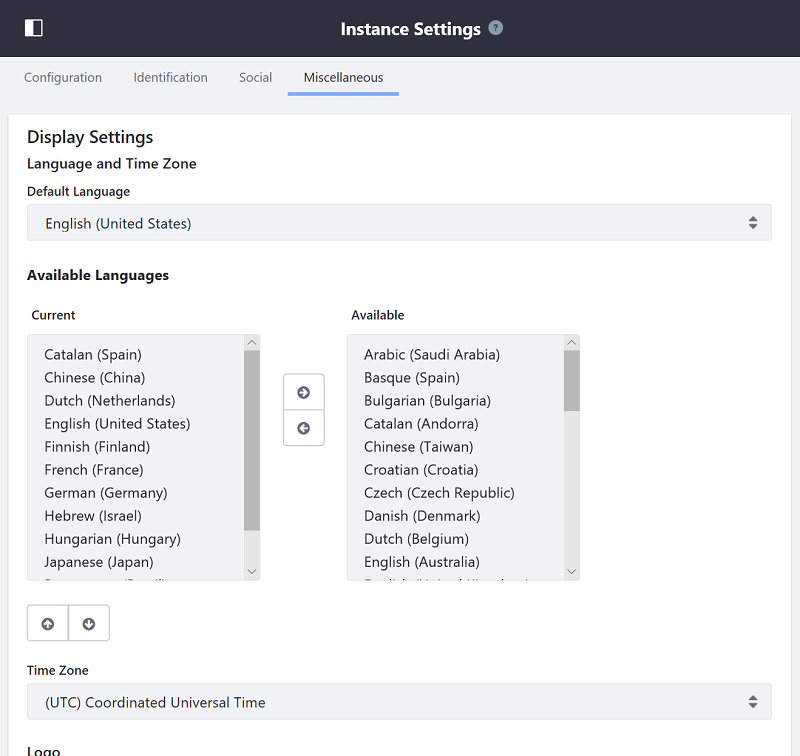
\includegraphics{./images/instance-locales.png}
\caption{You can change the default and available languages and the time
zone in Instance Settings.}
\end{figure}

Using the central left and right arrows, administrators can add or
remove available languages and locales. You can also modify these
properties in your \texttt{portal-ext.properties} file. You'll find them
in the
\href{@platform-ref@/7.0-latest/propertiesdoc/portal.properties.html\#Company}{Company}
section:

\begin{verbatim}
company.default.locale=en_GB
\end{verbatim}

As an example, the above property changes the locale to English, Great
Britain.

\subsection{Set the JVM Time Zone to
GMT}\label{set-the-jvm-time-zone-to-gmt}

It is possible to set time zones at the JVM level. However, users will
encounter issues such as Calendar Events and Web Content articles
displaying the wrong dates. This happens because the system assumes each
date stored in the database is stored in GMT time. When the system needs
to display one stored date to the end users, Liferay DXP calculates the
display date based on the current date of the \emph{application server}.
This date is affected by the configured JVM level time zone and the
stored GMT format date. In order to make sure the display date is
calculated correctly, the time zone must be configured to GMT at the JVM
level. Otherwise, it will result in incorrect time zone offset and cause
the display date to be wrongly calculated and displayed.

\subsection{Friendly URLs and
Locales}\label{friendly-urls-and-locales}

In addition to configuring Liferay DXP's instance settings, users can
also provide unique URLs for specific languages using the
\texttt{I18nServlet} by editing Liferay DXP's \texttt{web.xml} file:

\begin{verbatim}
<servlet-mapping>
    <servlet-name>I18n Servlet</servlet-name>
    <url-pattern>/ar/*</url-pattern>
</servlet-mapping>
.
.
.
<servlet-mapping>
    <servlet-name>I18n Servlet</servlet-name>
    <url-pattern>/de/*</url-pattern>
</servlet-mapping>
\end{verbatim}

The defaults that Liferay provides should be sufficient for nearly all
circumstances. Because this requires stopping and possibly redeploying
Liferay DXP (depending on your app server), test the defaults and make
sure you really need to modify these settings. If you're clustered, you
must make these changes on all nodes.

\subsection{Modifying Language Keys}\label{modifying-language-keys}

Developers can add or modify certain core UI messages (e.g.~\emph{Your
request completed successfully.}) by
\href{/docs/7-0/tutorials/-/knowledge_base/t/overriding-language-keys\#modifying-global-language-keys}{modifying
the language keys} that ship by default.

\subsection{Right to Left}\label{right-to-left}

For languages that are displayed right to left, modify the
\texttt{language.properties} using the following properties:

\begin{verbatim}
lang.dir=rtl
lang.line.begin=right
lang.line.end=left
\end{verbatim}

\subsection{Localizing User Names}\label{localizing-user-names}

Users can change the prefix and suffix values for a locale. For example,
for Spanish, the \texttt{language\_es.properties} file contains these
values:

\begin{verbatim}
lang.user.name.field.names=prefix,first-name,last-name
lang.user.name.prefix.values=Sr,Sra,Sta,Dr,Dra
lang.user.name.required.field.names=last-name
\end{verbatim}

For more information, see
\href{/docs/7-0/tutorials/-/knowledge_base/t/using-liferays-language-settings}{Using
Liferay Language Settings}.

\subsection{Related Topics}\label{related-topics}

\href{/docs/7-0/tutorials/-/knowledge_base/t/using-liferays-language-settings}{Using
Liferay Language Settings}

\href{/docs/7-0/tutorials/-/knowledge_base/t/overriding-language-keys\#modifying-global-language-keys}{Modifying
Liferay DXP's Language Keys}

\href{/docs/7-0/tutorials/-/knowledge_base/t/overriding-language-keys\#overriding-a-modules-language-keys}{Overriding
a Module's Language Keys}

\section{Document Repository
Configuration}\label{document-repository-configuration}

There are several options available for configuring how Liferay DXP's
Documents and Media library stores files. Each option is a \emph{store}
which can be configured through the \texttt{portal-ext.properties} file
by setting the \texttt{dl.store.impl=} property.

By default, Liferay DXP uses a document library store option called
Simple File Store to store documents and media files on a file system
(local or mounted). The store's default root folder is
\texttt{{[}Liferay\ Home{]}/data/document\_library}. You can specify a
different root directory from within
\href{/docs/7-0/user/-/knowledge_base/u/system-settings}{System
Settings}. To access System Settings, open the \emph{Menu}
(
\includegraphics{./images/icon-menu.png}) and navigate to
\emph{Control Panel → Configuration → System Settings}. From System
Settings, navigate to \emph{Foundation} and then search for and select
the entry \emph{Simple File System Store}. For the store's \emph{Root
dir} value, specify a path relative to
\href{/docs/7-0/deploy/-/knowledge_base/d/installing-product\#liferay-home}{Liferay
Home} or an absolute path; then click the \emph{Update} button. The
document library store switches immediately to the new folder.

You can also use an entirely different method for storing documents and
media files:

\textbf{Simple File System Store}: uses the file system (local or a
mounted share) to store files.

\textbf{Advanced File System Store}: in addition to using the file
system (local or a mounted share) to store files, Advanced File System
Store nests the files into more directories by version, for faster
performance and to store more files. separate from Liferay DXP to store
files.

\textbf{DBStore (Database Storage)}: stores files in the Liferay DXP
database.

\textbf{S3Store (Amazon Simple Storage)}: uses Amazon's cloud-based
storage solution.

\textbf{CMIS Store (deprecated as of Liferay DXP Digital Enterprise 7.0
Fix Pack 14 (SP3) and Liferay Portal CE 7.0 GA4)}: uses a system

\textbf{JCRStore (deprecated as of Liferay DXP Digital Enterprise 7.0
Fix Pack 14 (SP3) and Liferay Portal CE 7.0 GA4)}: stores files to a
JSR-170 compliant document repository. You can use any JCR client to
access the files. The files are stored to the server's file system by
default. You can optionally configure JCRStore to store files in a
database.

Here are the details for each one.

\subsection{Using the File System
Store}\label{using-the-file-system-store}

This is the default store. It's a simple file storage implementation
that uses a local folder to store files. You can use the file system for
your clustered configuration, but you'd have to make sure the folder to
which you point the store can handle things like concurrent requests and
file locking. For this reason, you need to use a Storage Area Network or
a clustered file system.

The file system store was the first store created for Liferay DXP and is
heavily bound to the Liferay DXP database. By default, documents are
stored in a \texttt{document\_library} subfolder of the \texttt{data}
folder in a Liferay DXP bundle. Of course, you can change this path to
anything you want in System Settings.

This store creates a folder structure based on primary keys in the
Liferay DXP database. If, for example, you upload a presentation with
the file name \texttt{workflow.odp} into a folder called \emph{stuff},
the file system store creates a folder structure that looks like the
figure below.

The folder path used by Liferay DXP for storing documents is this:

\begin{verbatim}
/companyId/folderId/numericFileEntryName/versionNumber
\end{verbatim}

The first folder name is the company ID to which the site belongs. The
second folder name is the Documents and Media folder's ID where the
document resides. The third folder name is the document's numeric file
entry name. Finally, the fourth name is a version number used for
storing multiple versions of the document.

\noindent\hrulefill

\textbf{Note:} A document's numeric file entry name is distinct from the
document ID; be careful not to confuse the two! Each has an independent
counter. The numeric file entry name is used in the folder path for
storing the document but the document ID is not. The numeric file entry
name can be found in the \texttt{name} column of the
\texttt{DLFileEntry} table in Liferay DXP's database; the document ID
can be found in the \texttt{fileEntryId} column of the same table.

\noindent\hrulefill

As you can see, the File System Store binds your documents very closely
to Liferay DXP, and may not be exactly what you want. If you've been
using the default settings for a while and need to migrate your
documents, Liferay DXP provides a migration utility in the Control Panel
in \emph{Server Administration} → \emph{Data Migration}. Using this
utility, you can move your documents very easily from one store
implementation to another.

\subsection{Using the Advanced File System
Store}\label{using-the-advanced-file-system-store}

Liferay DXP's advanced file system store is similar to the default file
system store. Like that store, it saves files to the local file
system--which, of course, could be a remote file system mount. It uses a
slightly different folder structure to store files, which is pictured
below.

\begin{figure}
\centering
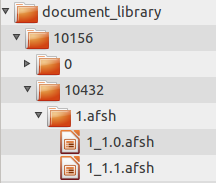
\includegraphics{./images/enterprise-adv-file-system-store.png}
\caption{The advanced file system store creates a more nested folder
structure than the file system store.}
\end{figure}

So what makes the advanced file system store \emph{advanced}? Several
operating systems have limitations on the number of files which can be
stored in a particular folder. The advanced file system store overcomes
this limitation by programmatically creating a structure that can expand
to millions of files, by alphabetically nesting the files in folders.
This not only allows for more files to be stored, but also improves
performance as there are fewer files stored per folder.

The same rules apply to the advanced file system store as apply to the
default file system store. To cluster this, you must point the store to
a network mounted file system that all the nodes can access, and that
networked file system must support concurrent requests and file locking.
Otherwise, you may experience data corruption issues if two users
attempt to write to the same file at the same time from two different
nodes.

\noindent\hrulefill

\textbf{Note:} Since Liferay DXP 7.0 Fix Pack 14 and Liferay Portal 7.0
CE GA4, to configure the advanced file system store you must configure
both the \texttt{portal-ext.properties} and \texttt{.config} files.

\noindent\hrulefill

Create the following file inside your app server's \texttt{osgi/configs}
folder:

\begin{verbatim}
com.liferay.portal.store.file.system.configuration.AdvancedFileSystemStoreConfiguration.cfg
\end{verbatim}

\noindent\hrulefill

\textbf{Note:} you can also generate the config file by exporting the
configurations from the Control Panel under \emph{System Settings} →
\emph{Foundation} → \emph{Advanced File System Store}.

\noindent\hrulefill

Configure the property shown below:

Property \textbar{} Default \textbar{} Required \texttt{rootDir}
\textbar{} \texttt{data/document\_library} \textbar{} \texttt{true}

\textbf{You may need to update the} \texttt{rootDir} \textbf{property to
correctly reflect where your document library is stored}.

Next, configure \texttt{portal-ext.properties}:

\begin{verbatim}
dl.store.impl=com.liferay.portal.store.file.system.AdvancedFileSystemStore
\end{verbatim}

With both the \texttt{.config} file and \texttt{portal-ext.properties}
configured, you can start Liferay DXP.

You may decide the advanced file system store for whatever reason
doesn't serve your needs. If this is the case, you can of course mount
other file systems into the documents and media library. In addition to
this, you can also redefine the Liferay DXP store to use one of three
other supported protocols. We'll look at these next.

\subsection{Using Amazon Simple Storage
Service}\label{using-amazon-simple-storage-service}

Amazon's simple storage service (S3) is a cloud-based storage solution
that you can use with Liferay DXP. All you need is an account, and you
can store your documents to the cloud from all nodes, seamlessly.

When you sign up for the service, Amazon assigns you unique keys that
link you to your account. In Amazon's interface, you can create
``buckets'' of data optimized by region. Once you've created these to
your specifications, use
\href{/docs/7-0/deploy/-/knowledge_base/d/document-repository-configuration\#s3}{these
instructions} to connect your S3 account to Liferay DXP.

If you are using Tomcat as your app server, it doesn't contain a
\texttt{SAXParser}. You must include this property in
\texttt{system-ext.properties}:

\begin{verbatim}
org.xml.sax.driver=com.sun.org.apache.xerces.internal.parsers.SAXParser
\end{verbatim}

Other app servers also need this configuration if they don't contain a
\texttt{SAXParser}. Remember to place your
\texttt{system-ext.properties} file in a folder that resides in your
Liferay DXP installation's class path (e.g.,
\texttt{/WEB-INF/classes/}).

\noindent\hrulefill

\textbf{Note:} No action is required to support AWS Signature Version 4
request authorization.

\noindent\hrulefill

Consult the Amazon Simple Storage documentation for additional details
on using Amazon's service.

\subsection{Using the CMIS Store}\label{using-the-cmis-store}

Though you can mount as many different CMIS (Content Management
Interoperability Services) repositories as you like in the Documents and
Media library, you may wish also to redefine the Liferay DXP repository
to point to a CMIS repository as well. Why? Users might want to create a
folder or upload content to the Liferay DXP repository. It would be nice
if that Liferay DXP repository was connected to a clustered CMIS
repository by the administrator without having to mount it through the
UI. The CMIS store allows you to do just that.

\noindent\hrulefill

\textbf{Note:} CMIS Store is not suitable for production use and is
deprecated as of Liferay DXP Digital Enterprise 7.0 Fix Pack 14 (SP3)
and Liferay Portal CE 7.0 GA4. Because it can have performance issues
with large repositories, it's recommended that you use one of the other
configuration repositories listed above, such as Advanced File System
Store, to store your Documents and Media files. This deprecation does
not affect the use of external repositories. You can still
\href{/docs/7-0/user/-/knowledge_base/u/using-external-repositories}{connect
to external repositories} using CMIS.

\noindent\hrulefill

If you wish to use the CMIS store, follow the instructions
\href{/docs/7-0/deploy/-/knowledge_base/d/document-repository-configuration\#cmis-store}{here}
to set it up. The Liferay DXP repository is connected to CMIS via the
CMIS store. As long as all nodes are pointing to your CMIS repository,
everything in your Liferay DXP cluster should be fine, as the CMIS
protocol prevents multiple simultaneous file access from causing data
corruption.

\subsection{Using the JCR Store}\label{using-the-jcr-store}

Liferay DXP supports as a store the Java Content Repository standard.
Under the hood, Liferay DXP uses Jackrabbit, a project from Apache, as
its JSR-170 compliant document repository. By default, Jackrabbit is
configured to store the documents on the local file system where Liferay
DXP is installed, in the \texttt{{[}Liferay\ Home{]}/liferay/jackrabbit}
folder. Inside this folder is Jackrabbit's configuration file, called
\texttt{repository.xml}.

\noindent\hrulefill

\textbf{Note:} JCR Store is deprecated as of Liferay DXP Digital
Enterprise 7.0 Fix Pack 14 (SP3) and Liferay Portal CE 7.0 GA4. You
should use one of the other documentation repositories listed above.

\noindent\hrulefill

Using the default settings, the JCR store is not very different from the
file system stores, except you can use any JCR client to access the
files. You can, however, modify Jackrabbit's configuration so it stores
files in a database that can be accessed by all nodes, and so that it
operates as a cluster within Liferay DXP's cluster.

To move the default repository location to a shared folder, you do not
need to edit Jackrabbit's configuration file. Instead, follow the
instructions
\href{/docs/7-0/deploy/-/knowledge_base/d/document-repository-configuration\#jcr}{here}.
Change it to point to a shared folder that all the nodes can see. A new
Jackrabbit configuration file is then generated in that location, and
you'll have to edit that file to modify Jackrabbit's configuration.

Note that because of file locking issues, this isn't the best way to
share Jackrabbit resources, unless you're using a networked file system
that can handle concurrency and file locking. If you have two people
logged in at the same time uploading content, you could encounter data
corruption using this method, and because of this, we don't recommend it
for a production system. Instead, if you want to use the Java Content
Repository in a cluster, you should redirect Jackrabbit into your
database of choice. You can use the Liferay DXP database or another
database for this purpose. This requires editing Jackrabbit's
configuration file.

The default Jackrabbit configuration file has sections commented out for
moving the Jackrabbit configuration into the database. This has been
done to make it as easy as possible to enable this configuration. To
move the Jackrabbit configuration into the database, comment out the
sections relating to the file system and comment in the sections
relating to the database. These by default are configured for a MySQL
database. If you are using another database, you will need to modify the
configuration, as there are changes to the configuration file that are
necessary for specific databases. For example, the default configuration
uses Jackrabbit's \texttt{DbFileSystem} class to mimic a file system in
the database. While this works well in MySQL, it doesn't work for all
databases. For example, an Oracle database requires the
\texttt{OracleFileSystem}.

Modify the JDBC database URLs so they point to your database. This, of
course, must be done on all nodes of the cluster. Don't forget to create
the database first and grant the user ID you are specifying in the
configuration file access to create, modify, and drop tables. After
this, be sure to uncomment the
\texttt{\textless{}Cluster/\textgreater{}} section at the bottom of the
file. For further information, it's best to check out the
\href{http://jackrabbit.apache.org}{Jackrabbit documentation}.

Once you've configured Jackrabbit to store its repository in a database,
the next time you bring up Liferay DXP, the necessary database tables
are created automatically. Jackrabbit, however, does not create indexes
on these tables, and so over time this can be a performance penalty. To
fix this, you must manually go into your database and index the primary
key columns for all the Jackrabbit tables.

Note that this configuration doesn't perform as well as the advanced
file system store, because you're storing documents in a database
instead of on the file system. But it does have the benefit of
clustering well. For example, you can store documents and media files in
your Liferay DXP instance's database using DBStore. To enable DBStore,
add the following
\href{@platform-ref@/7.0-latest/propertiesdoc/portal.properties.html\#Document\%20Library\%20Service}{\texttt{dl.store.impl}}
portal property to a \texttt{portal-ext.properties} file in your
\href{/docs/7-0/deploy/-/knowledge_base/d/installing-product\#liferay-home}{Liferay
Home}:

\begin{verbatim}
dl.store.impl=com.liferay.portal.store.db.DBStore
\end{verbatim}

Remember to restart your Liferay DXP server after updating your
\texttt{portal-ext.properties} file in order for your customizations to
take effect.

\subsection{Configuration Details}\label{configuration-details}

There are properties related to document library stores that have been
moved from \texttt{portal-ext.properties} to OSGi configuration files.
The following mapping shows you how to configure those properties if
needed:

\subsection{File Store}\label{file-store}

From \texttt{portal-ext.properties}:
\texttt{dl.store.impl=com.liferay.portal.store.file.system.FileSystemStore}

To
\texttt{osgi/configs/com.liferay.portal.store.file.system.configuration.FileSystemStoreConfiguration.cfg}:

Property \textbar{} Default \textbar{} Required \texttt{rootDir}
\textbar{} \texttt{data/document\_library} \textbar{} \texttt{false}

\subsection{Advanced File Store}\label{advanced-file-store}

\textbf{Since Liferay DXP 7.0 Fix Pack 14 and Liferay Portal 7.0 CE GA4,
both the \texttt{portal-ext.properties} and \texttt{.config} files are
required to configure the advanced file system store.}

From \texttt{portal-ext.properties}:
\texttt{dl.store.impl=com.liferay.portal.store.file.system.AdvancedFileSystemStore}

To
\texttt{osgi/configs/com.liferay.portal.store.file.system.configuration.AdvancedFileSystemStoreConfiguration.cfg}:

Property \textbar{} Default \textbar{} Required \texttt{rootDir}
\textbar{} \texttt{data/document\_library} \textbar{} \texttt{true}

\subsection{S3}\label{s3}

From \texttt{portal-ext.properties}:
\texttt{dl.store.impl=com.liferay.portal.store.s3.S3Store}

To
\texttt{osgi/configs/com.liferay.portal.store.s3.configuration.S3StoreConfiguration.cfg}:

Property \textbar{} Default \textbar{} Required \texttt{accessKey}
\textbar{} \textbar{} \texttt{false} \texttt{secretKey} \textbar{}
\textbar{} \texttt{false} \texttt{s3Region} \textbar{}
\texttt{us-east-1} \textbar{} \texttt{false} \texttt{bucketName}
\textbar{} \textbar{} \texttt{true} \texttt{s3StorageClass} \textbar{}
STANDARD \textbar{} \texttt{false} \texttt{httpClientMaxConnections}
\textbar{} \texttt{50} \textbar{} \texttt{false}
\texttt{cacheDirCleanUpExpunge} \textbar{} \texttt{7} \textbar{}
\texttt{false} \texttt{cacheDirCleanUpFrequency} \textbar{} \texttt{100}
\textbar{} \texttt{false}

\noindent\hrulefill

\textbf{Note:} Amazon S3 requires a SAXParser from the application
server to operate. For some application servers (e.g.~Tomcat), it's
necessary to define a SAXParser in order to prevent errors while
utilizing this store. This may be set in \texttt{system-ext.properties}.
For example,

\begin{verbatim}
 org.xml.sax.driver=com.sun.org.apache.xerces.internal.parsers.SAXParser
\end{verbatim}

\textbf{Warning:} If a database transaction rollback occurs in a
Document Library that uses a file system based store, file system
changes that have occurred since the start of the transaction won't be
reversed. Inconsistencies between Document Library files and those in
the file system store can occur and may require manual synchronization.
All stores except DBStore are vulnerable to this limitation.

\noindent\hrulefill

\subsection{CMIS Store}\label{cmis-store}

From \texttt{portal-ext.properties}:
\texttt{dl.store.impl=com.liferay.portal.store.cmis.CMISStore}

To
\texttt{osgi/configs/com.liferay.portal.store.cmis.configuration.CMISStoreConfiguration.cfg}:

Property \textbar{} Default \textbar{} Required \texttt{repositoryUrl}
\textbar{} \texttt{http://localhost:8080/alfresco/service/api/cmis}
\textbar{} \texttt{true} \texttt{credentialsUsername} \textbar{} none
\textbar{} \texttt{true} \texttt{credentialsPassword} \textbar{} none
\textbar{} \texttt{true} \texttt{systemRootDir} \textbar{} Liferay Home
\textbar{} \texttt{true}

\subsection{JCR}\label{jcr}

From \texttt{portal-ext.properties}:
\texttt{dl.store.impl=com.liferay.portal.store.jcr.JCRStore}

To
\texttt{osgi/configs/com.liferay.portal.store.jcr.configuration.JCRStoreConfiguration.cfg}:

Property \textbar{} Default \textbar{} Required
\texttt{initializeOnStartup} \textbar{} \texttt{false}\textbar{}
\texttt{true} \texttt{wrapSession} \textbar{} \texttt{true} \textbar{}
\texttt{true} \texttt{moveVersionLabels} \textbar{} \texttt{false}
\textbar{} \texttt{true} \texttt{workspaceName} \textbar{}
\texttt{liferay} \textbar{} \texttt{true} \texttt{nodeDocumentlibrary}
\textbar{} \texttt{documentlibrary} \textbar{} \texttt{true}
\texttt{jackrabbitRepositoryRoot} \textbar{} \texttt{data/jackrabbit}
\textbar{} \texttt{true} \texttt{jackrabbitConfigFilePath} \textbar{}
\texttt{repository.xml} \textbar{} \texttt{true}
\texttt{jackrabbitRepositoryHome} \textbar{} \texttt{home} \textbar{}
\texttt{true} \texttt{jackrabbitCredentialsUsername} \textbar{} none
\textbar{} \texttt{true} \texttt{jackrabbitCredentialsPassword}
\textbar{} none \textbar{} \texttt{true}

\noindent\hrulefill

\textbf{Note:} Use the absolute path for
\texttt{jackrabbitRepositoryRoot}, \texttt{jackrabbitConfigFilePath},
and \texttt{jackrabbitRepositoryHome}.

\noindent\hrulefill

Please refer to the
\href{@platform-ref@/7.0-latest/propertiesdoc/portal.properties.html\#Document\%20Library\%20Portlet}{Document
Library property reference} for a complete list of supported
customizations. You can customize features such as the maximum allowed
size of documents and media files, the list of allowed file extensions,
which types of files should be indexed, and more.

\section{Liferay DXP Clustering}\label{liferay-dxp-clustering}

Liferay DXP can serve everything from the smallest to the largest web
sites. Out of the box, it's configured optimally for a single server
environment. If one server isn't sufficient to serve the high traffic
needs of your site, Liferay DXP scales to the size you need.

\begin{figure}
\centering
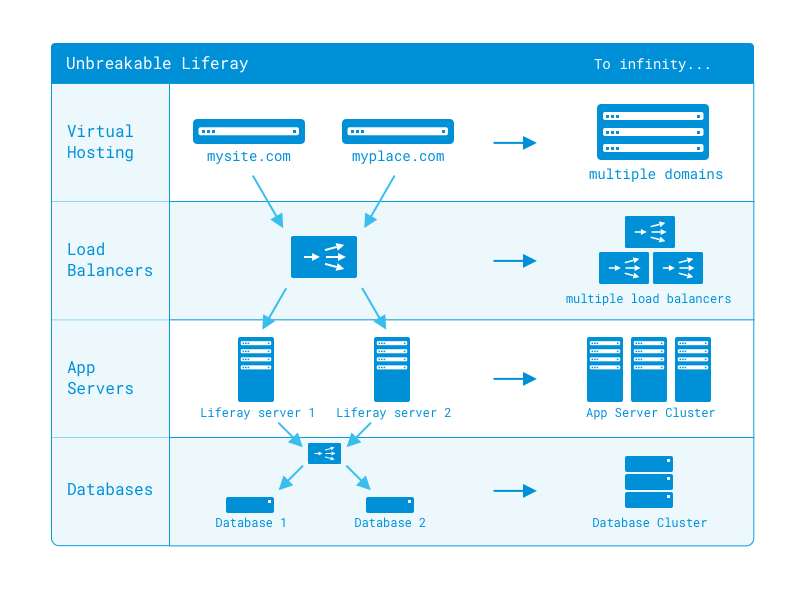
\includegraphics{./images-dxp/clustering-enterprise-configuration.png}
\caption{Liferay DXP is designed to scale to as large an installation as
you need.}
\end{figure}

Liferay DXP works well in clusters of multiple machines (horizontal
cluster) or in clusters of multiple VMs on a single machine (vertical
cluster), or any mixture of the two. Once you have Liferay DXP installed
in more than one application server node, there are several
optimizations that need to be made. At a minimum, Liferay DXP should be
configured in the following way for a clustered environment:

\begin{enumerate}
\def\labelenumi{\arabic{enumi}.}
\item
  All nodes should be pointing to the same Liferay DXP database or
  database cluster.
\item
  Documents and Media repositories must have the same configuration and
  be accessible to all nodes of the cluster.
\item
  Search should be on a separate search server that is optionally
  clustered.
\item
  Cluster Link must be enabled so the cache replicates across all nodes
  of the cluster.
\item
  Hot deploy applications to each node individually.
\end{enumerate}

If you haven't configured your application server to use farms for
deployment, the hot deploy folder should be a separate folder for all
the nodes, and plugins will have to be deployed to all of the nodes
individually. This can be done via a script. If you do have farms
configured, you can deploy normally to any node's deploy folder, and
your farm configuration should take care of syncing the deployment to
all nodes.

Many of these configuration changes can be made by adding or modifying
properties in your \texttt{portal-ext.properties} file. Remember that
this file overrides the defaults in the \texttt{portal.properties} file.
You can also browse its contents
\href{https://docs.liferay.com/digital-enterprise/7.0-latest/propertiesdoc/portal.properties.html}{here}.
It's a best practice to copy the relevant section you want to modify
from \texttt{portal.properties} into your \texttt{portal-ext.properties}
file, and then modify the values there.

\noindent\hrulefill

\textbf{Note:} This article documents a Liferay DXP-specific cluster
configuration without getting into specific implementations of third
party software, such as Java EE application servers, HTTP servers, and
load balancers. Please consult your documentation for those components
of your cluster to configure those components. Before creating a Liferay
DXP cluster, make sure your OS is not defining the hostname of your box
to the local network at 127.0.0.1.

\noindent\hrulefill

Each step defined above is covered below to give you a step by step
process for creating your cluster.

\subsection{1. All Nodes Should Point to the Same Liferay DXP
Database}\label{all-nodes-should-point-to-the-same-liferay-dxp-database}

Each node should have a data source that points to one Liferay DXP
database (or a database cluster) that all the nodes will share. This
means, of course, Liferay DXP cannot (and should not) use the embedded
HSQL database that is shipped with the bundles (but you already knew
that, right?). And, of course, the database server should be on a
separate system from the server which is running Liferay DXP.

You can also use a read-writer database configuration to optimize your
database configuration.

\subsection{Read-Writer Database
Configuration}\label{read-writer-database-configuration}

Liferay DXP allows you to use two different data sources for reading and
writing. This enables you to split your database infrastructure into two
sets: one optimized for reading and one optimized for writing. Since all
Liferay DXP's supported databases support replication, you can use your
database vendor's replication mechanism to keep the database nodes in
sync.

Enabling a read-writer database is simple. In your
\texttt{portal-ext.properties} file:

\begin{enumerate}
\def\labelenumi{\arabic{enumi}.}
\item
  Set the default database connection pool provider to \texttt{dbcp},
  \texttt{tomcat}, or \texttt{c3po}. Note, provider HikariCP does not
  support read/write splitting. Here's an example setting:

\begin{verbatim}
jdbc.default.liferay.pool.provider=dbcp
\end{verbatim}

  All the portal JDBC configuration properties are documented
  \href{@platform-ref@/7.0-latest/propertiesdoc/portal.properties.html\#JDBC}{here}.
\item
  Configure two different data sources for Liferay DXP to use, one for
  reading, and one for writing:

\begin{verbatim}
jdbc.read.driverClassName=com.mysql.jdbc.Driver
jdbc.read.url=jdbc:mysql://dbread.com/lportal?useUnicode=true&characterEncoding=UTF-8&useFastDateParsing=false
jdbc.read.username=**your user name**
jdbc.read.password=**your password**

jdbc.write.driverClassName=com.mysql.jdbc.Driver
jdbc.write.url=jdbc:mysql://dbreadwrite.com/lportal?useUnicode=true&characterEncoding=UTF-8&useFastDateParsing=false
jdbc.write.username=**your user name**
jdbc.write.password=**your password**
\end{verbatim}

  To use the JNDI instead of the JDBC data sources, set the
  \texttt{*.username} and \texttt{*.password} properties above to your
  JNDI user name and password and set these additional properties:

\begin{verbatim}
jdbc.read.jndi.name=**your read JNDI name**
jdbc.write.jndi.name=**your read-write JNDI name**
\end{verbatim}
\item
  Avoid using the \texttt{default} data source, by setting this:

\begin{verbatim}
counter.jdbc.prefix=jdbc.write.
\end{verbatim}

  And if you're using a \texttt{dbcp} or \texttt{tomcat} database
  connection pool provider, set these:

\begin{verbatim}
jdbc.default.validationQuery=
jdbc.read.validationQuery=SELECT releaseId FROM Release_
jdbc.write.validationQuery=SELECT releaseId FROM Release_
\end{verbatim}

  These settings are related to issue
  \href{https://issues.liferay.com/browse/LPS-64624}{LPS-64624}.
\item
  Enable the read-writer database configuration by uncommenting the
  following Spring configuration files from the \texttt{spring.configs}
  and \texttt{spring.infrastructure.configs} properties:

\begin{verbatim}
spring.configs=\
    [..]
    META-INF/dynamic-data-source-spring.xml,\
    [..]

spring.infrastructure.configs=\
    [..]
    META-INF/dynamic-data-source-infrastructure-spring.xml,\
    [..]
\end{verbatim}

  The Spring configuration portal properties are documented
  \href{@platform-ref@/7.0-latest/propertiesdoc/portal.properties.html\#Spring}{here}.
\end{enumerate}

The next time you start Liferay DXP, it uses the two data sources you
have defined. Be sure you have correctly set up your two databases for
replication before starting Liferay DXP.

\subsection{2. Documents and Media Library
Clustering}\label{documents-and-media-library-clustering}

Liferay DXP's Documents and Media Library can mount several repositories
at a time while presenting a unified interface to the user. By default,
users can use the Liferay DXP repository, which is already mounted. This
repository is built into Liferay DXP and can use one of
\href{/docs/7-0/deploy/-/knowledge_base/d/document-repository-configuration}{several
different store implementations} as its back-end. In addition to this,
users can mount many different kinds of third party repositories. In a
cluster, Documents and Media must have the exact same configuration on
all nodes. If you have a separate repository you've mounted, all nodes
of the cluster must point to this repository. Your avenue for improving
performance at this point is to cluster your third party repository,
using the documentation for the repository you have chosen. If you don't
have a third party repository, you can configure the Liferay DXP
repository to perform well in a clustered configuration.

The main thing to keep in mind is you need to make sure that every node
of the cluster has the same access to the file store as every other
node. For this reason, you must look at your store configuration.

Note that the file systems used by the \texttt{File\ System} or
\texttt{Advanced\ File\ System} stores must support concurrent requests
and file locking.

\noindent\hrulefill

\textbf{Checkpoint}: To test if the sharing works well, execute the
following steps:

\begin{enumerate}
\def\labelenumi{\arabic{enumi}.}
\tightlist
\item
  On Node 1 upload a document to the Documents and Media.
\item
  On Node 2 download the document. The download should be successful.
\item
  Repeat the test with reversed roles.
\end{enumerate}

\noindent\hrulefill

\subsection{3. Clustering Search}\label{clustering-search}

Search should always run on a separate environment from your Liferay DXP
server. Liferay DXP supports
\href{/docs/7-0/deploy/-/knowledge_base/d/configuring-elasticsearch-for-liferay-0}{Elasticsearch}
or \href{/docs/7-0/deploy/-/knowledge_base/d/using-solr}{Solr}, and
either of those environments can also be clustered.

For more information on how to cluster Elasticsearch, see
\href{https://www.elastic.co/guide/en/elasticsearch/guide/current/distributed-cluster.html}{Elasticsearch's
distributed cluster setup}.

Once Liferay DXP servers have been properly configured as a cluster and
the same for Elasticsearch, change Liferay DXP from \emph{embedded} mode
to \emph{remote} mode. On the first connection, the two sets of
clustered servers communicate with each other the list of all IP
addresses; in case of a node going down, the proper failover protocols
will enable. Queries and indices can continue to be sent for all nodes.

For more information on how to cluster Solr, see
\href{https://cwiki.apache.org/confluence/display/solr/SolrCloud}{Apache
Solr Cloud} documentation.

Once Liferay DXP servers have been properly configured as a cluster,
deploy the Liferay Solr 5 Adapter on all nodes. (This app is available
for download from Liferay Marketplace
\href{https://web.liferay.com/marketplace/-/mp/application/78803813}{here}.)
Create a Solr Cloud (cluster) managed by \emph{Apache Solr Zookeeper}.
Connect the Liferay DXP cluster to Zookeeper and finish the final
configurations to connect the two clusters.

\subsection{4. Enable Cluster Link}\label{enable-cluster-link}

Enabling Cluster Link automatically activates distributed caching.
Distributed caching enables some RMI (Remote Method Invocation) cache
listeners that are designed to replicate the cache across a cluster.
Cluster Link uses \href{http://www.ehcache.org}{Ehcache}, which has
robust distributed caching support. The cache is distributed across
multiple Liferay DXP nodes running concurrently. The Ehcache global
settings are in the
\href{@platform-ref@/7.0-latest/propertiesdoc/portal.properties.html\#Ehcache}{\texttt{portal.properties}
file}.

By default Liferay does not copy cached entities between nodes. If an
entity is deleted or changed, for example, Cluster Link sends an
\emph{remove} message to the other nodes to invalidate this entity in
their local cache. Requesting that entity on another node results in a
cache \emph{miss}; the entity is then retrieved from the database and
put into the local cache. Entities added to one node's local cache are
not copied to local caches of the other nodes. An attempt to retrieve a
new entity on a node which doesn't have that entity cached results in a
cache \emph{miss}. The miss triggers the node to retrieve the entity
from the database and store it in its local cache.

\begin{figure}
\centering
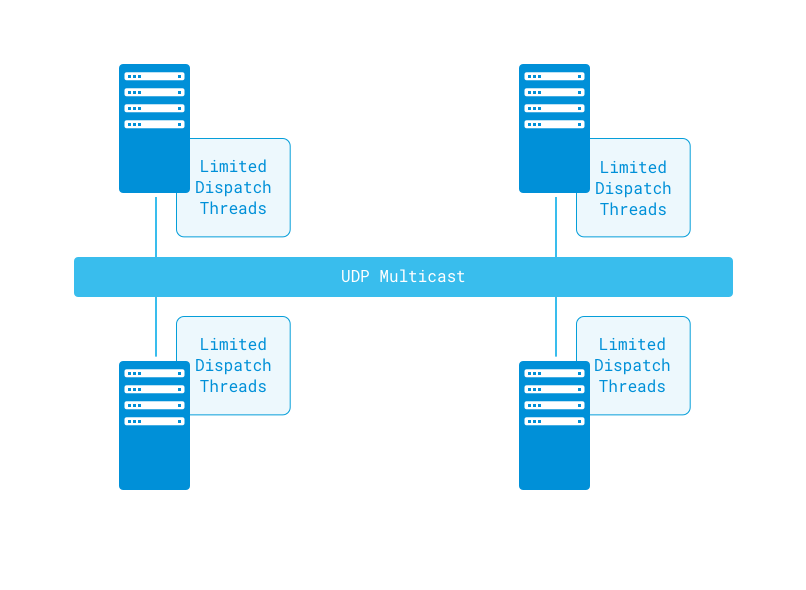
\includegraphics{./images-dxp/clustering-cache-efficient-algorithm.png}
\caption{Liferay DXP's cache algorithm is extremely efficient.}
\end{figure}

To enable Cluster Link, add this property to
\texttt{portal-ext.properties}:

\begin{verbatim}
cluster.link.enabled=true
\end{verbatim}

Cluster Link depends on \href{http://www.jgroups.org}{JGroups}, and
provides an API for nodes to communicate. It can

\begin{itemize}
\tightlist
\item
  Send messages to all nodes in a cluster
\item
  Send messages to a specific node
\item
  Invoke methods and retrieve values from all, some, or specific nodes
\item
  Detect membership and notify when nodes join or leave
\end{itemize}

When you start @portal@ in a cluster, a log file message shows your
cluster's name (e.g., \texttt{cluster=liferay-channel-control}):

\begin{verbatim}
------------------------------------------------------------------- 
GMS: address=oz-52865, cluster=liferay-channel-control, physical address=192.168.1.10:50643 
-------------------------------------------------------------------
\end{verbatim}

Cluster Link contains an enhanced algorithm that provides one-to-many
type communication between the nodes. This is implemented by default
with JGroups's UDP multicast, but unicast and TCP are also available.

\subsection{Multicast over UDP}\label{multicast-over-udp}

When you enable Cluster Link, Liferay DXP's default clustering
configuration is enabled. This configuration defines IP multicast over
UDP. Liferay DXP uses two groups of
\href{http://www.jgroups.org/manual/index.html\#_channel}{channels from
JGroups} to implement this: a control group and a transport group. If
you want to customize the channel properties, you can do so in
\texttt{portal-ext.properties}:

\begin{verbatim}
cluster.link.channel.name.control=[your control channel name]
cluster.link.channel.properties.control=[your control channel properties]
\end{verbatim}

Please see
\href{http://www.jgroups.org/manual/index.html\#protlist}{JGroups's
documentation} for channel properties. The default configuration sets
many properties whose settings are discussed there.

Multicast broadcasts to all devices on the network. Clustered
environments on the same network communicate with each other by default.
Messages and information (e.g., scheduled tasks) sent between them can
lead to unintended consequences. Isolate such cluster environments by
either separating them logically or physically on the network, or by
configuring each cluster's \texttt{portal-ext.properties} to use
different sets of
\href{https://docs.liferay.com/portal/7.0-latest/propertiesdoc/portal.properties.html\#Multicast}{multicast
group address and port values}.

JGroups sets a bind address automatically, using \texttt{localhost} by
default. In some configurations, however, \texttt{localhost} is bound to
the internal loopback network (\texttt{127.0.0.1} or \texttt{::1}),
rather than the host's real address. As long as DXP's
\texttt{cluster.link.autodetect.address} Portal Property points to a
server that's contactable, DXP uses that server to automatically detect
your host's real address. Here's the default setting:

\begin{verbatim}
cluster.link.autodetect.address=www.google.com:80
\end{verbatim}

Contacting Google may not work if your server is behind a firewall.

An alternative to detecting the host address automatically for the bind
address, you can set the bind address manually in your
\texttt{portal-ext.properties} file.

\begin{enumerate}
\def\labelenumi{\arabic{enumi}.}
\item
  Disable address auto-detection by setting the
  \texttt{cluster.link.autodetect.address} property to an empty value:

\begin{verbatim}
cluster.link.autodetect.address=
\end{verbatim}
\item
  Set the following properties to your host's IP address:

\begin{verbatim}
cluster.link.bind.addr["cluster-link-control"]=[place your IP address or host name here]
cluster.link.bind.addr["cluster-link-udp"]=[place your IP address or host name here]
\end{verbatim}
\end{enumerate}

Your network configuration may preclude the use of multicast over TCP,
so below are some other ways you can get your cluster communicating.
Note that these methods are all provided by JGroups.

Checkpoint:

\begin{enumerate}
\def\labelenumi{\arabic{enumi}.}
\item
  If you are binding the IP address instead of using \texttt{localhost},
  make sure the right IP addresses are declared using:

  \texttt{cluster.link.bind.addr{[}"cluster-link-control"{]}=localhost}\strut \\
  \texttt{cluster.link.bind.addr{[}"cluster-link-udp"{]}=localhost}
\item
  Test your load and then optimize your settings if necessary.
\end{enumerate}

\subsection{Unicast over TCP}\label{unicast-over-tcp}

If your network configuration or the sheer distance between nodes
prevents you from using UDP Multicast clustering, you can configure
Liferay DXP to use TCP Unicast. You'll definitely need this if you have
a firewall separating any of your nodes or if your nodes are in
different geographical locations.

\begin{enumerate}
\def\labelenumi{\arabic{enumi}.}
\item
  Add a parameter to your app server's JVM:

\begin{verbatim}
-Djgroups.bind_addr=[place your IP address or host name here]
\end{verbatim}

  Use the node's IP address or host name.
\item
  Now you have to determine the discovery protocol the nodes should use
  to find each other. You have four choices:

\begin{verbatim}
- TCPPing
- JDBCPing
- S3_Ping
- Rackspace_Ping
\end{verbatim}

  If you aren't sure which one to choose, use TCPPing. This is used in
  the rest of these steps; the others are covered below.
\item
  Download the latest
  \texttt{com.liferay.portal.cluster.multiple-{[}version{]}.jar} file
  from
  \href{https://repository.liferay.com/nexus/content/repositories/liferay-public-releases/com/liferay/com.liferay.portal.cluster.multiple}{Liferay's
  Nexus repository}. In this JAR's \texttt{lib} folder is a file called
  \texttt{jgroups-{[}version{]}.Final.jar}. Open it and find
  \texttt{tcp.xml}. Extract this file to a location accessible to
  Liferay DXP. Use this file on all your nodes.
\item
  If you're vertically clustering (i.e., you have multiple Liferay DXP
  servers running on the same physical or virtual system), you must
  change the port on which discovery communicates for all nodes other
  than the first one, to avoid TCP port collision. To do this, modify
  the TCP tag's \texttt{bind\_port} parameter:

\begin{verbatim}
<TCP bind_port="[some unused port]"
    ... 
/>
\end{verbatim}

  Since the default port is \texttt{7800}, provide some other unused
  port.
\item
  Add to the same tag the parameter
  \texttt{singleton\_name="liferay\_cluster"}. This merges the transport
  and control channels to reduce the number of thread pools. See
  \href{http://www.jgroups.org/manual-3.x/html/user-advanced.html}{JGroups
  documentation} for further information.

  Usually, no further JGroups configuration is required. However, in a
  very specific case, if \emph{(and only if)} cluster nodes are deployed
  across multiple networks, then the parameter \texttt{external\_addr}
  must be set on each host to the external (public IP) address of the
  firewall. This kind of configuration is usually only necessary when
  nodes are geographically separated. By setting this, clustered nodes
  that are deployed to separate networks (e.g.~separated by different
  firewalls) can communicate together. This configuration will likely be
  flagged in security audits of your system. See
  \href{http://www.jgroups.org/manual-3.x/html/protlist.html\#Transport}{JGroups
  documentation} for more information.
\item
  Save the file. Modify that node's \texttt{portal-ext.properties} file
  to point to it:

\begin{verbatim}
cluster.link.channel.properties.control=[CONFIG_FILE_PATH]/tcp.xml
cluster.link.channel.properties.transport.0=[CONFIG_FILE_PATH]/tcp.xml
\end{verbatim}
\end{enumerate}

You're now set up for Unicast over TCP clustering! Repeat this process
for each node you want to add to the cluster.

\subsubsection{JDBC Ping}\label{jdbc-ping}

Rather than use TCP Ping to discover cluster members, you can use a
central database accessible by all the nodes to help them find each
other. Cluster members write their own and read the other members'
addresses from this database. To enable this configuration, replace the
\texttt{TCPPING} tag with the corresponding \texttt{JDBCPING} tag:

\begin{verbatim}
<JDBC_PING
    connection_url="jdbc:mysql://[DATABASE_IP]/[DATABASE_NAME]?useUnicode=true&amp;characterEncoding=UTF-8&amp;useFastDateParsing=false"
    connection_username="[DATABASE_USER]"
    connection_password="[DATABASE_PASSWORD]"
    connection_driver="com.mysql.jdbc.Driver"/>
\end{verbatim}

The above example uses MySQL as the database. For further information
about JDBC Ping, please see the
\href{http://www.jgroups.org/manual-3.x/html/protlist.html\#DiscoveryProtocols}{JGroups
Documentation}.

\subsubsection{S3 Ping}\label{s3-ping}

Amazon S3 Ping can be used for servers running on Amazon's EC2 cloud
service. Each node uploads a small file to an S3 bucket, and all the
other nodes read the files from this bucket to discover the other nodes.
When a node leaves, its file is deleted.

To configure S3 Ping, replace the \texttt{TCPPING} tag with the
corresponding \texttt{S3\_PING} tag:

\begin{verbatim}
<S3_PING 
    secret_access_key="[SECRETKEY]" 
    access_key="[ACCESSKEY]"
    location="ControlBucket"/>
\end{verbatim}

Supply your Amazon keys as values for the parameters above. For further
information about S3 Ping, please see the
\href{http://www.jgroups.org/manual-3.x/html/protlist.html\#DiscoveryProtocols}{JGroups
Documentation}.

\subsubsection{Other Pings}\label{other-pings}

JGroups supplies other means for cluster members to discover each other,
including Rackspace Ping, BPing, File Ping, and others. Please see the
\href{http://www.jgroups.org/manual-3.x/html/protlist.html\#DiscoveryProtocols}{JGroups
Documentation} for information about these discovery methods.

\subsection{Modifying the Cache Configuration with a
Module}\label{modifying-the-cache-configuration-with-a-module}

It's recommended to test your system under a load that best simulates
the kind of traffic your system needs to handle. If you'll be serving up
a lot of message board messages, your script should reflect that. If web
content is the core of your site, your script should reflect that too.

As a result of a load test, you may find that the default distributed
cache settings aren't optimized for your site. In this case, you should
tweak the settings yourself. You can modify the Liferay DXP installation
directly or you can use a module to do it. Either way, the settings you
change are the same. A benefit of working with modules is that you can
install a module on each node and change the settings without taking
down the cluster. Modifying the Ehcache settings with a module is
recommended over modifying the Ehcache settings directly.

We've made this as easy as possible by
\href{https://portal.liferay.dev/documents/113763090/114000186/portal-cache-override-config.zip}{creating
the project} for you. Download the project and unzip it into a
\href{/docs/7-0/tutorials/-/knowledge_base/t/liferay-workspace}{Liferay
Workspace}, in the workspace's \texttt{modules} folder. To override your
cache settings, you only have to modify one Ehcache configuration file,
which you'll find inside the \texttt{src/main/java} folder structure:

\begin{itemize}
\tightlist
\item
   resources

  \begin{itemize}
  \tightlist
  \item
    ehcache

    \begin{itemize}
    \tightlist
    \item
      override-liferay-multi-vm-clustered.xml
    \end{itemize}
  \end{itemize}
\end{itemize}

In the sample project, this file contains a configuration for Liferay
DXP's \texttt{GroupImpl} object which handles sites. You may wish to add
other objects to the cache; in fact, the default file caches many other
objects. For example, if you have a vibrant community, a large portion
of your traffic may be directed at the message boards portlet, as in the
example above. To cache the threads on the message boards, configure a
block with the \texttt{MBMessageImpl} class:

\begin{verbatim}
<cache
    eternal="false"
    maxElementsInMemory="10000"
    name="com.liferay.portlet.messageboards.model.impl.MBMessageImpl"
    overflowToDisk="false"
    timeToIdleSeconds="600"
>
</cache>
\end{verbatim}

If you're overriding these properties, it's because you want to
customize the configuration for your own site. A good way to start with
this is to extract Liferay's cluster configuration file and then
customize it. You'll find it in the Liferay Foundation application
suite's \texttt{com.liferay.portal.ehcache-{[}version{]}.jar} file. You
can get this JAR from the \texttt{Liferay\ Foundation.lpkg} file in the
\texttt{osgi/marketplace} folder. The file you want is
\texttt{liferay-multi-vm-clustered.xml}, in the \texttt{/ehcache} folder
inside the \texttt{com.liferay.portal.ehcache-{[}version{]}.jar} file.
Once you have the file, replace the contents of the
\texttt{override-liferay-multi-vm-clustered.xml} file above with the
contents of this file. Now you'll be using the default configuration as
a starting point.

Once you've made your changes to the cache, save the file, build, and
deploy the module, and your settings override the default settings. In
this way, you can tweak your cache settings so that your cache performs
optimally for the type of traffic generated by your site. You don't have
restart your server to change the cache settings. This is a great
benefit, but beware: since Ehcache doesn't allow for changes to cache
settings while the cache is alive, reconfiguring a cache while the
server is running flushes the cache.

\subsection{5. Hot Deploy to All
Nodes}\label{hot-deploy-to-all-nodes}

If you want to deploy any module or WAR file onto the cluster, it must
be deployed to all nodes of the cluster. Because Liferay DXP now
\href{/docs/7-0/tutorials/-/knowledge_base/t/using-the-wab-generator}{installs
applications as OSGi bundles}, this means you cannot rely on your
application server's means of installing WAR files (even if you only
intend to install WAR files) to deploy an application to the entire
cluster. Instead, the application must be placed in Liferay DXP's
\texttt{deploy} folder on each node.

This, as you might imagine, can be done with a script. Write a shell
script that uploads applications to each node using sftp or some other
service. This way, when you deploy an application, it is uploaded to
each node's \texttt{deploy} folder and installed by each running Liferay
DXP installation.

\subsection{Summary}\label{summary}

Setting up Liferay DXP on a cluster takes five steps:

\begin{enumerate}
\def\labelenumi{\arabic{enumi}.}
\item
  Point all nodes at the same database or database cluster.
\item
  Make sure the Documents and Media repository is accessible to all
  nodes.
\item
  Install Elasticsearch or Solr on a separate system or cluster.
\item
  Enable Cluster Link for cache replication.
\item
  Hot deploy applications to each node individually.
\end{enumerate}

\chapter{Updating a Cluster}\label{updating-a-cluster}

Maintaining a
\href{/docs/7-0/deploy/-/knowledge_base/d/liferay-clustering}{cluster}
is a big responsibility. It includes deploying new and updated modules
and plugins, applying fixes and improvements, making configuration
changes, and more. Maximizing server uptime and minimizing risks take
priority when applying changes. Liferay DXP supports
\href{/docs/7-0/deploy/-/knowledge_base/d/other-cluster-update-techniques}{standard
cluster maintenance techniques}, such as
\href{/docs/7-0/deploy/-/knowledge_base/d/using-rolling-restarts}{rolling
restarts}.

You should use rolling restarts if possible as it maximizes uptime and
mitigates risks of changes harming your deployment.
\href{/docs/7-0/deploy/-/knowledge_base/d/other-cluster-update-techniques}{Other
techniques} include

\begin{itemize}
\tightlist
\item
  Cluster code changes.
\item
  Non-revertible
  \href{/docs/7-0/deploy/-/knowledge_base/d/maintaining-liferay}{fix
  packs}.
\item
  Module/plugin data changes (modifying data in existing columns).
\item
  Module/plugin data schema changes that break compatibility with the
  existing version. Breaking changes include but are not limited to
  dropping columns, changing column types, and changing data formats
  used in columns (such as changing from XML to JSON).
\item
  Updating a data schema to a version outside of a Service Builder
  service module's
  \href{/docs/7-0/tutorials/-/knowledge_base/t/creating-an-upgrade-process-for-your-app\#specifying-the-schema-version}{required
  data schema range}.
\end{itemize}

Since eligible changes should be done with rolling restarts, it's
explained first.

\section{Using Rolling Restarts}\label{using-rolling-restarts}

A rolling restart is shutting down and updating nodes one at a time
(while the other nodes are running) until they're all updated. This
keeps your site running while you update your cluster, whether it's
physical, container, or image based.

Here's how a rolling restart works:

\begin{enumerate}
\def\labelenumi{\arabic{enumi}.}
\item
  Shut down one cluster node (JVM instance).
\item
  Update/modify the deployment for that node (see the maintenance
  scenarios that follow).
\item
  Start the node.
\item
  Repeat these steps for all other cluster nodes.
\end{enumerate}

User experience can be inconsistent during a rolling restart. For
example, UI changes in a plugin update are only visible on the updated
nodes. Users on nodes that haven't been updated see the old interface.
Maintenance scenarios might have specific cases that cannot be performed
in rolling restarts. The scenario descriptions mention these cases.

The maintenance scenarios eligible for rolling restarts are described
below.

\subsection{New Modules and Plugins}\label{new-modules-and-plugins}

For a new plugin or module (one that does not already exist in the
cluster) to be eligible for rolling restart it must not modify data,
delete, or rename database columns in a way that breaks compatibility
with existing plugins or modules.

\subsection{Updating Existing Modules and
Plugins}\label{updating-existing-modules-and-plugins}

For a new version of an existing plugin or module to be eligible for
rolling restart, it must not modify data or delete or rename database
columns in a way that breaks compatibility with the existing version of
the plugin or module.

\subsection{Applying Fix Packs (DXP
only)}\label{applying-fix-packs-dxp-only}

The Customer Portal identifies
\href{/docs/7-0/deploy/-/knowledge_base/d/maintaining-liferay}{fix
packs} that are not revertible, and therefore ineligible for rolling
restart. All other fix packs are eligible.

\subsection{Reverting Fix Packs (DXP
only)}\label{reverting-fix-packs-dxp-only}

Revertible fix packs can be removed in rolling restarts.

\subsection{\texorpdfstring{Portal Properties controlled by
\texttt{portal-ext.properties}}{Portal Properties controlled by portal-ext.properties}}\label{portal-properties-controlled-by-portal-ext.properties}

\href{@platform-ref@/7.1-latest/propertiesdoc/portal.properties.html}{Portal
Properties} file changes can be applied in rolling restarts.

\subsection{System Settings controlled by Configuration Admin
Files}\label{system-settings-controlled-by-configuration-admin-files}

\href{/docs/7-0/user/-/knowledge_base/u/understanding-system-configuration-files}{System
configuration} files can be applied in rolling restarts.

\subsection{Application Server or JVM setting
modifications}\label{application-server-or-jvm-setting-modifications}

Modifications to application server and JVM settings can be done in
rolling restarts.

\subsection{Java Version Updates}\label{java-version-updates}

Minor version updates of Java can be applied in rolling restarts. Major
version updates are not supported in rolling restarts, and should
instead be done when all cluster nodes are shut down.

All rolling restart-eligible updates can be applied using the rolling
restart steps listed above. Other updates must be done differently as
described next.

\subsection{Related Topics}\label{related-topics-1}

\href{/docs/7-0/deploy/-/knowledge_base/d/liferay-clustering}{Liferay
DXP Clustering}

\href{/docs/7-0/deploy/-/knowledge_base/d/maintaining-liferay}{Maintaining
Liferay DXP}

\href{/docs/7-0/tutorials/-/knowledge_base/t/data-upgrades-and-verifiers}{Implementing
Data Upgrades}

\section{Other Cluster Update
Techniques}\label{other-cluster-update-techniques}

Several update scenarios cannot be done by
\href{/docs/7-0/deploy/-/knowledge_base/d/using-rolling-restarts}{rolling
restart} because they affect cluster communication, break compatibility
with existing plugins/modules, or break Service Builder services. Also
non-revertible updates are disqualified because reversing their effects
requires restoring data from a
\href{/docs/7-0/deploy/-/knowledge_base/d/backing-up-a-liferay-installation}{backup}.

Maintenance changes ineligible for rolling restart are typically done on
all nodes at once, when they're shut down. The following sections
describe techniques for applying these changes.

\begin{itemize}
\tightlist
\item
  Custom Plugin/Module Data Schema Changes
\item
  Custom Plugin/Module Data Changes
\item
  Non-revertible Fix Packs (DXP only)
\item
  Service Builder Service Schema Version Changes
\item
  Cluster Code Changes
\end{itemize}

Data schema changes are explained first.

\subsection{Custom Module/Plugin Data Schema
Changes}\label{custom-moduleplugin-data-schema-changes}

Custom module/plugin data schema changes that break compatibility with
existing modules and plugins must be introduced over several releases in
which the data is transitioned and maintained in old and new columns
until the old column is no longer needed.

\subsection{Custom Module/Plugin Data
Changes}\label{custom-moduleplugin-data-changes}

Data changes to modules or plugins you've developed require these steps:

\begin{enumerate}
\def\labelenumi{\arabic{enumi}.}
\item
  Create a new column.
\item
  Copy the data to the new column.
\item
  Maintain both columns until the old column is no longer used by any
  cluster nodes.
\item
  Delete the column in the next release.
\end{enumerate}

\subsection{Non-revertible Fix Packs (DXP
only)}\label{non-revertible-fix-packs-dxp-only}

The Customer Portal identifies fix packs that are not revertible.
Non-revertible fix packs must be applied to nodes when they are all shut
down.

\subsection{Service Builder Service Schema Version
Changes}\label{service-builder-service-schema-version-changes}

A module's \texttt{Liferay-Require-SchemaVersion} (specified in its
\texttt{bnd.bnd}) must match the module's schema version value in the
\texttt{Release\_} table. Installing a new module that has a new schema
version updates the \texttt{Release\_} table with that schema version
and triggers a data upgrade process. If you install such a module on one
node, the schema version in the \texttt{Release\_} table no longer
matches the \texttt{Liferay-Require-SchemaVersion} of the modules on the
other nodes. The module's Service Builder services become unavailable.
Such changes cannot be reverted: the database must be restored from a
backup. These schema version changes must be applied while all nodes are
shut down.

\subsection{Cluster Code Changes}\label{cluster-code-changes}

Cluster communication must stay intact. For this reason, cluster code
must not be updated in rolling restarts. The Customer Portal identifies
DXP fix packs that contain such changes as non-revertible. Here are
packages you must not change in rolling restarts:

\begin{itemize}
\tightlist
\item
  \texttt{com.liferay.portal.kernel.cluster}
\item
  \texttt{com.liferay.portal.kernel.cluster.*}
\item
  \texttt{com.liferay.portal.kernel.exception.NoSuchClusterGroupException}
\item
  \texttt{com.liferay.portal.kernel.scheduler.multiple}
\item
  \texttt{com.liferay.portal.kernel.scheduler.multiple.*}
\item
  \texttt{com.liferay.portal.cache.multiple}
\item
  \texttt{com.liferay.portal.cache.multiple.*}
\item
  \texttt{com.liferay.portal.scheduler.multiple}
\item
  \texttt{com.liferay.portal.scheduler.multiple.*}
\end{itemize}

Now you know how to update your cluster using ways other than rolling
restart.

\subsection{Related Topics}\label{related-topics-2}

\href{/docs/7-0/deploy/-/knowledge_base/d/liferay-clustering}{Liferay
DXP Clustering}

\href{/docs/7-0/deploy/-/knowledge_base/d/maintaining-liferay}{Maintaining
Liferay DXP}

\href{/docs/7-0/tutorials/-/knowledge_base/t/data-upgrades-and-verifiers}{Implementing
Data Upgrades}

\section{Configuring Remote Staging in a Clustered
Environment}\label{configuring-remote-staging-in-a-clustered-environment}

If you're running Liferay DXP as a
\href{/docs/7-0/deploy/-/knowledge_base/d/liferay-clustering}{clustered
environment} and you want to use remote staging, you must configure it
properly for a seamless experience. In this tutorial, you'll learn how
to set up remote staging in an example clustered environment scenario.
The example environment assumes you have

\begin{itemize}
\tightlist
\item
  A Staging instance with database configurations and a file repository
  different from the cluster nodes
\item
  A balancer responsible for managing the traffic flow between the
  cluster's nodes
\item
  Two nodes that call two Liferay app servers (e.g., \emph{App Server 1}
  and \emph{App Server 2}), both of which are connected to the same
  database
\end{itemize}

\begin{figure}
\centering
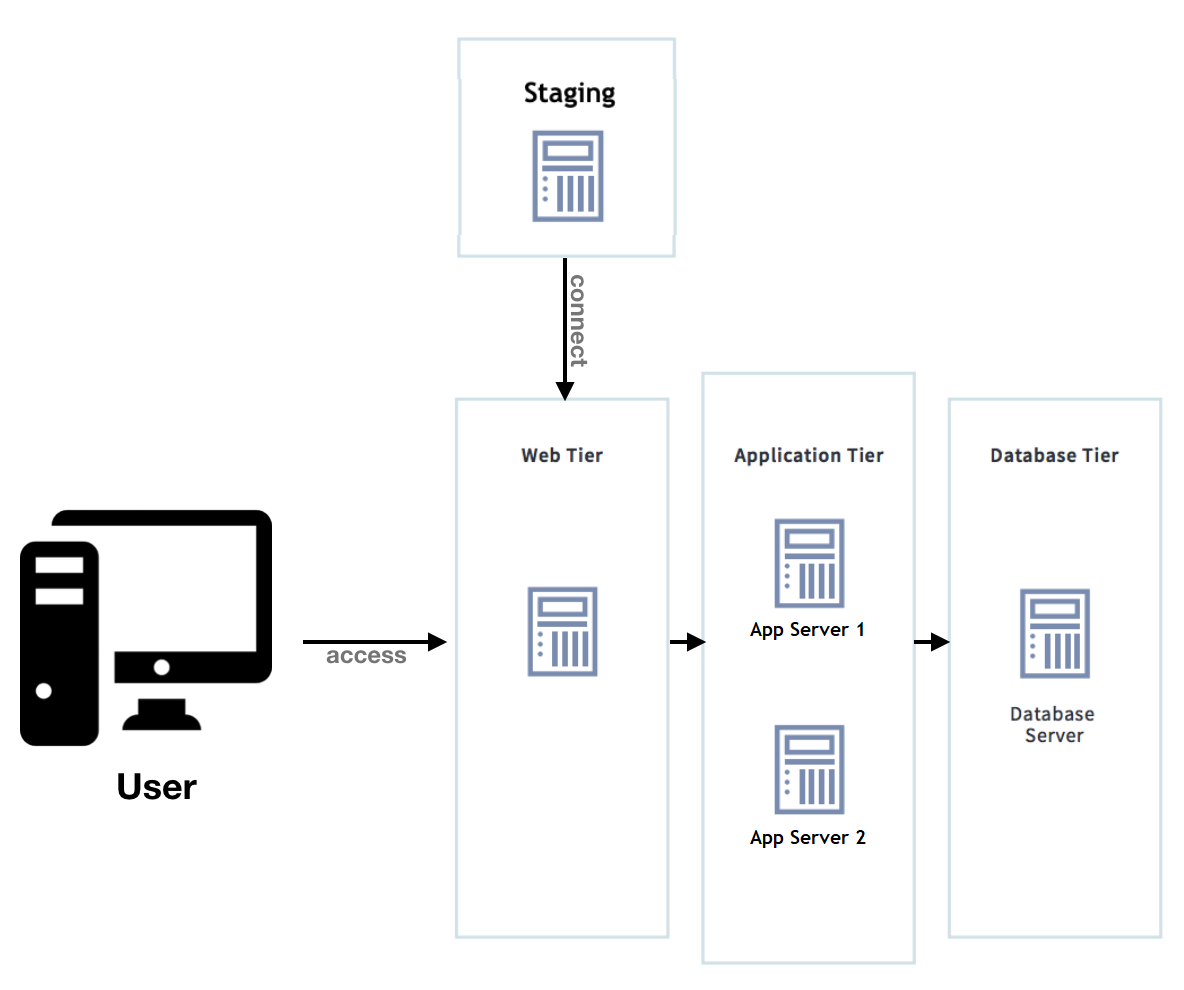
\includegraphics{./images/remote-staging-clustering.png}
\caption{This is the assumed setup for your clustered environment.}
\end{figure}

The steps below also assume your web tier, application tier, and cluster
environment are already configured. You may need to adjust the
configurations in this tutorial to work with your specific
configuration.

Let's begin!

\begin{enumerate}
\def\labelenumi{\arabic{enumi}.}
\item
  You must secure the communication made between your nodes and Staging
  server. Add the following property to both app servers' and Staging
  server's \texttt{portal-ext.properties} file:

\begin{verbatim}
tunneling.servlet.shared.secret=[secret]
\end{verbatim}

  This secret key denies other portals access to your configured portal
  servers. If you'd like to set your secret key using hexadecimal
  encoding, also set the following property in your
  \texttt{portal-ext.properties} files:

\begin{verbatim}
tunneling.servlet.shared.secret.hex=true
\end{verbatim}
\end{enumerate}

\noindent\hrulefill

\begin{verbatim}
 **Note:** The following key lengths are supported by the available
 encryption algorithms:
 
 - *AES:* 128, 192, and 256-bit keys
 - *Blowfish:* 32-448 bit keys
 - *DESede (Triple DES):* 56, 112, or 168 bit keys (Liferay places an
   artificial limit on the minimum key length and does not support the 56-bit
   key length)
 
 For example, you can use [OpenSSL](https://www.openssl.org/) to generate a
 128-bit AES key:
 
     openssl enc -aes-128-cbc -k abc123 -P -md sha1
\end{verbatim}

\noindent\hrulefill

\begin{enumerate}
\def\labelenumi{\arabic{enumi}.}
\setcounter{enumi}{1}
\item
  You must allow the connection between the configured IPs of your app
  servers and the Staging server. Open both of your app servers'
  \texttt{portal-ext.properties} files and add the following properties:

\begin{verbatim}
tunnel.servlet.hosts.allowed=127.0.0.1,SERVER_IP,[STAGING_IP]
tunnel.servlet.https.required=false
\end{verbatim}

  The \texttt{{[}STAGING\_IP{]}} variable must be replaced by the
  staging server's IP addresses. The \texttt{SERVER\_IP} constant can
  remain set for this property; it's automatically replaced by the
  Liferay server's IP addresses.
\item
  If you're validating IPv6 addresses, you must configure the app
  server's JVM to not force the usage of IPv4 addresses. For example, if
  you're using Tomcat, add the following attribute in the
  \texttt{\$TOMCAT\_HOME\textbackslash{}bin\textbackslash{}setenv.{[}bat\textbar{}sh{]}}
  file.

  \texttt{-Djava.net.preferIPv4Stack=false}
\item
  Restart both app servers for the new properties to take effect.
\item
  Configure the \emph{TunnelAuthVerifier} property for your nodes' app
  servers. There are two ways to do this:

  \begin{itemize}
  \item
    \textbf{Use a \texttt{.config} file (recommended):} In the
    \texttt{\$LIFERAY\_HOME/osgi/configs} folder of one of your node
    Liferay DXP instances, create (if necessary) a
    \texttt{com.liferay.portal.security.auth.verifier.tunnel.module.configuration.TunnelAuthVerifierConfiguration-default.config}
    file and insert the properties listed below. Creating one
    \texttt{.config} file configures all cluster nodes the same way. For
    more information on \texttt{.config} files, see the
    \href{/docs/7-0/user/-/knowledge_base/u/understanding-system-configuration-files}{Understanding
    System Configuration Files} article.

\begin{verbatim}
  enabled=true
  hostsAllowed=127.0.0.1,SERVER_IP,STAGING_IP
  serviceAccessPolicyName=SYSTEM_USER_PASSWORD
  urlsIncludes=/api/liferay/do
\end{verbatim}
  \item
    \textbf{Via System Settings:} Navigate to the \emph{Control Panel} →
    \emph{Configuration} → \emph{System Settings} → \emph{Foundation} →
    \emph{Tunnel Auth Verifiers}. Click on the \emph{/api/liferay/do}
    configuration entry and add the Staging IP address to the
    \emph{Hosts allowed} field. If you choose to configure the
    \emph{TunnelAuthVerifier} this way, you \textbf{must} do this for
    all nodes (e.g., App Server 1 and App Server 2).
  \end{itemize}
\item
  On your Staging instance, navigate to the Site Administration portion
  of the Product Menu and select \emph{Publishing} → \emph{Staging}.
  Then select \emph{Remote Live}.

  \begin{figure}
  \centering
  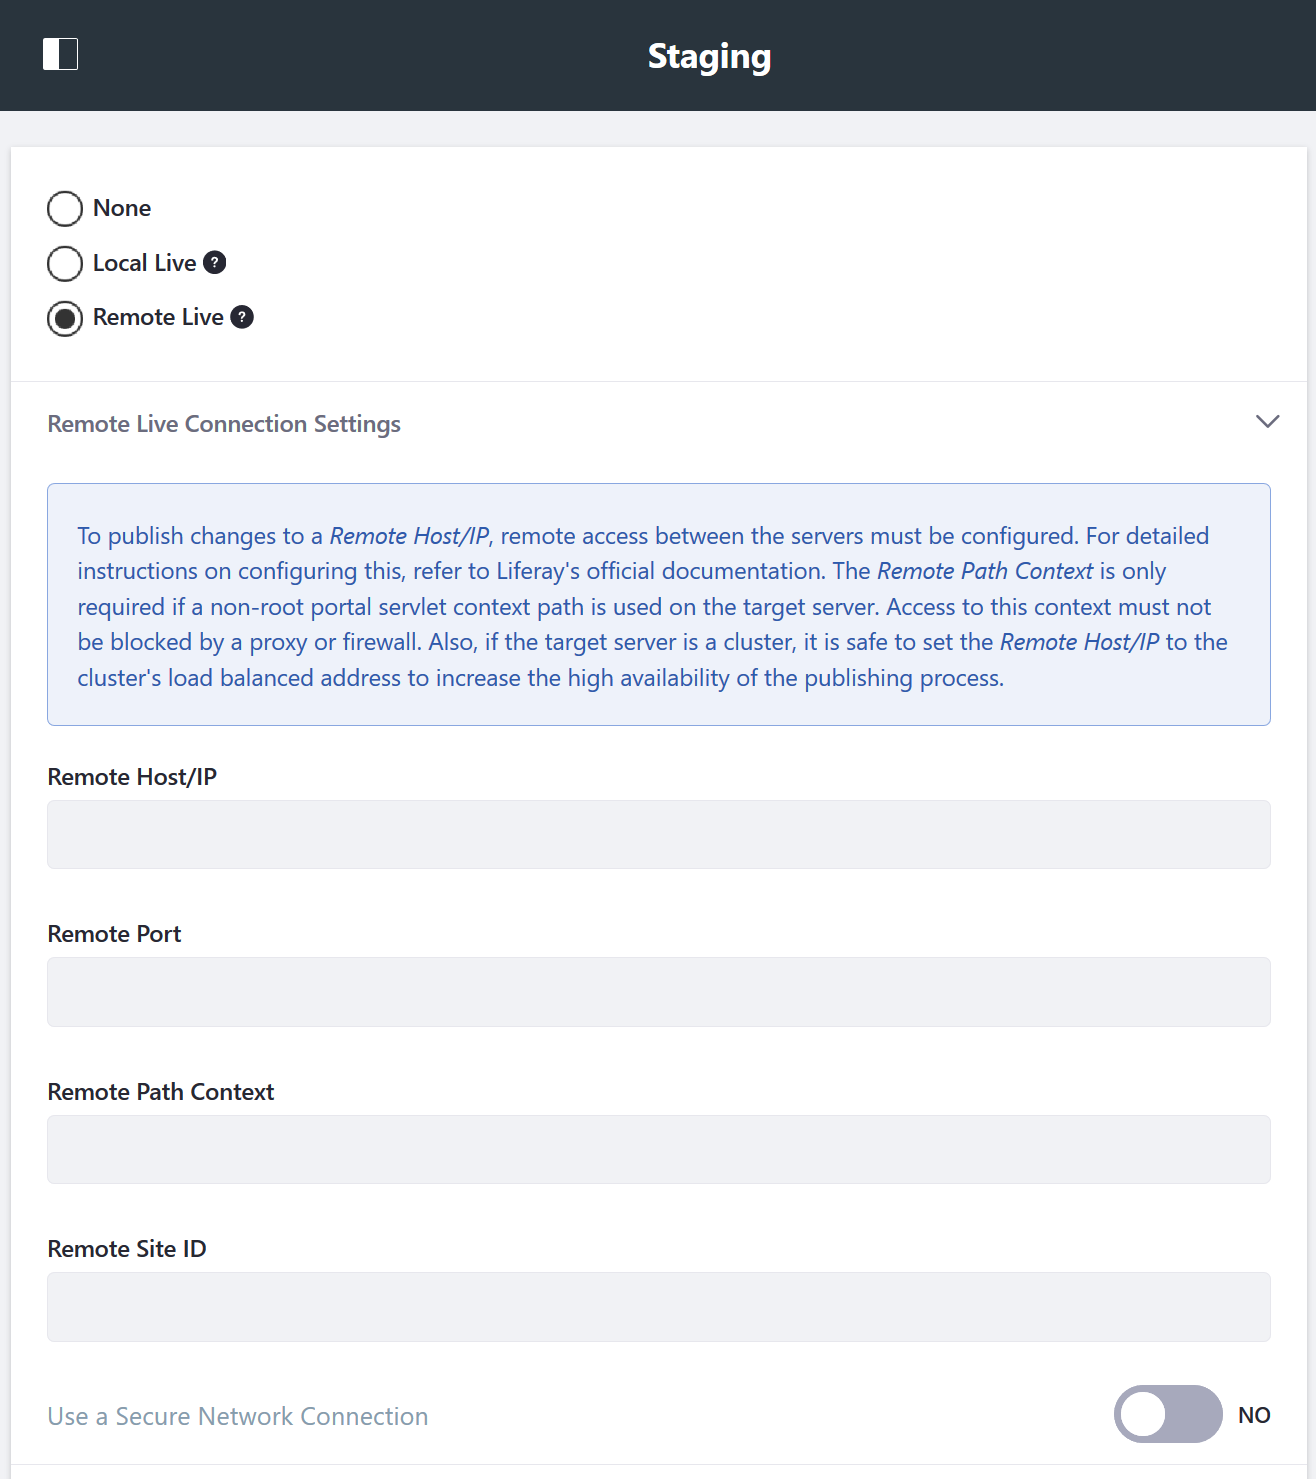
\includegraphics{./images/remote-staging-menu.png}
  \caption{When selecting the Remote Staging radio button, you're given
  a list of options to configure.}
  \end{figure}
\item
  For the Remote Host/IP field, insert the balancer's IP of your web
  tier. Configuring the Staging instance with the balancer's IP ensures
  the availability of the environment at the time of publication from
  staging to live.
\item
  Enter the port on which the balancer is running into the Remote Port
  field.
\item
  Insert the remote site ID of your app servers into the Remote Site ID
  field. The site ID of all your app servers are the same since they are
  configured for the same database and are shared between nodes.

  Navigate to the Site Administration portion of the Product Menu and
  select \emph{Site Settings} to find the site ID.
\item
  Save the Remote Live settings.
\end{enumerate}

That's it! You've configured remote staging in your clustered
environment.

\chapter{Liferay Digital Enterprise Configuration and Tuning
Guidelines}\label{liferay-digital-enterprise-configuration-and-tuning-guidelines}

When tuning Liferay DXP installation, there are several factors to take
into consideration; some are specific to Liferay DXP, while others are
concepts that apply to all Java and Java enterprise applications. The
following guidelines are meant to serve as an initial baseline from
which to tune your specific deployment.

\section{Application Server Tuning}\label{application-server-tuning}

Although the actual setting names may differ, these concepts are
applicable across most application servers. For brevity, we will use
Tomcat as an example. For other application servers, consult the
application server provider's documentation for additional specific
settings.

\subsection{Database Connection Pool}\label{database-connection-pool}

The database connection pool is usually sized at roughly 30-40\% of the
thread pool size. The connection pool provides a connection whenever
Liferay DXP needs to retrieve data from the database (e.g.~user login,
etc.). If this size is too small, requests queue in the server waiting
for database connections. Too large a setting, however, means wasting
resources with idle database connections.

As with thread pools, monitor these settings and adjust them based on
your performance tests.

In Tomcat, the connection pools are configured in the Resource elements
in \texttt{\$CATALINA\_HOME/conf/\ Catalina/localhost/ROOT.xml}. Liferay
Engineering uses the following configuration during testing:

\begin{verbatim}
<Resource auth="Container"         
    description="Digital Enterprise DB Connection"   
    driverClass="com.mysql.jdbc.Driver"   
    maxPoolSize="75"   minPoolSize="10"           
    acquireIncrement="5"   
    name="jdbc/LiferayPool"  
    user="XXXXXX"   
    password="XXXXXXXXX"           
    factory="org.apache.naming.factory.BeanFactory"
    type="com.mchange.v2.c3p0.ComboPooledDataSource"
    jdbcUrl="jdbc:mysql://someServer:3306/liferay_dxp?useUnicode=true
    &amp;characterEncoding=UTF-8&amp;useFastDateParsing=false"/>
\end{verbatim}

In this configuration, we start with 10 threads and increment by 5 as
needed to a maximum of 75 connections in the pool.

You may choose from a variety of database connection pool providers,
including DBCP, C3P0, HikariCP, and Tomcat. You may also choose to
configure the Liferay JDBC settings in your portal.properties.

\subsection{Deactivate Development Settings in the JSP
Engine}\label{deactivate-development-settings-in-the-jsp-engine}

Many application servers have their JSP Engines configured for
development mode by default. Liferay recommends deactivating these
settings prior to entering production:

\textbf{Development mode:} This makes the JSP container poll the file
system for changes to JSP files. Since you won't be making changes on
the fly like this in production, you should turn this off.

\textbf{Mapped File:} Generates static content with one print statement
versus one statement per line of JSP text.

To do this in Tomcat, you modify the
\texttt{\$CATALINA\_HOME/conf/web.xml} file. Update the JSP servlet to
look like the following configuration:

\begin{verbatim}
<servlet>   
    <servlet-name>jsp</servlet-name>
    <servlet-class>org.apache.jasper.servlet.JspServlet</servlet-class>   
    <init-param>    
        <param-name>development</param-name>    
        <param-value>false</param-value>   
    </init-param>   
    <init-param>    
        <param-name>mappedFile</param-name>    
        <param-value>false</param-value>   
    </init-param>   
    <load-on-startup>3</load-on-startup> 
</servlet>
\end{verbatim}

\subsection{Thread Pool}\label{thread-pool}

Each incoming request to the application server consumes a worker thread
for the duration of the request. When no threads are available to
process requests, the request is queued to wait for the next available
worker thread. In a finely tuned system, the number of threads in the
thread pool should be balanced with the total number of concurrent
requests. There should not be a significant amount of threads left idle
to service requests.

Liferay Engineering recommends an initial setting of 50 threads and then
monitoring it within your application server's monitoring consoles. You
may wish to use a higher number (e.g., 250) if your average page times
are in the 2-3 seconds range. Too few threads in the thread pool may
lead to excessive request queuing while too many threads may lead to
excessive context switching.

In Tomcat, the thread pools are configured in the Connector element in
\texttt{\$CATALINA\_HOME/conf/server.xml}. Further information can be
found in the
\href{https://tomcat.apache.org/tomcat-8.0-doc/config/http.html}{Apache
Tomcat documentation}. Liferay Engineering used the following
configuration during testing:

\begin{verbatim}
<Connector maxThreads="75" minSpareThreads="50" 
    maxConnections="16384" port="8080"     
    connectionTimeout="600000" redirectPort="8443" 
    URIEncoding="UTF-8"  socketBuffer="-1"     
    maxKeepAliveRequests="-1" address="xxx.xxx.xxx.xxx"/>
\end{verbatim}

Additional tuning parameters around Connectors are available, including
the connector types, the connection timeouts, and TCP queue. Consult the
appropriate Tomcat documentation for further details.

\section{Java Virtual Machine
Tuning}\label{java-virtual-machine-tuning}

Tuning the JVM primarily focuses on tuning the garbage collector and the
Java memory heap. These parameters are used to optimize the throughput
of your application. We used Oracle's 1.8 JVM for the reference
architecture. You may also choose other supported JVM versions and
implementations. Please consult the
\href{https://web.liferay.com/group/customer/dxp/support/compatibility-matrix}{Liferay
Digital Enterprise Compatibility Matrix} for additional compatible JVMs.

\subsection{Garbage Collector}\label{garbage-collector}

Choosing the appropriate garbage collector (GC) helps improve the
responsiveness of your Liferay DXP deployment. Liferay recommends using
the concurrent low pause collectors:

\begin{verbatim}
-XX:+UseParNewGC -XX:ParallelGCThreads=16 -XX:+UseConcMarkSweepGC
-XX:+CMSParallelRemarkEnabled -XX:+CMSCompactWhenClearAllSoftRefs
-XX:CMSInitiatingOccupancyFraction=85 -XX:+CMSScavengeBeforeRemark
\end{verbatim}

You may choose from other available GC algorithms including parallel
throughput collectors and G1 collectors. Liferay recommends first
starting your tuning using parallel collectors in the new generation and
concurrent mark sweep (CMS) in the old generation.

\textbf{Note:} the value 16 in \texttt{ParallelGCThreads=16} varies
based on the type of CPUs available. We recommend setting the value
according to CPU specification. On Linux machines, you may find the
number of available CPUs by running \texttt{cat\ /proc/cpuinfo}.

\textbf{Note:} There are additional ``new'' algorithms like G1, but
Liferay Engineering's tests for G1 have indicated that it does not
improve performance. Your application performance may vary and you
should add it to your testing and tuning plans.

\subsection{Code Cache}\label{code-cache}

Java uses a just-in-time (JIT) compiler that generates native code to
improve performance. The default size is 48M. This may not be sufficient
for larger applications. Too small a code cache reduces performance as
the JIT isn't able to optimize high frequency methods. For Digital
Enterprise, we recommend starting with 64M for the initial code cache
size.

\begin{verbatim}
-XX:InitialCodeCacheSize=32m -XX:ReservedCodeCacheSize=96m
\end{verbatim}

You can examine the efficacy of the parameter changes by adding the
following parameters:

\begin{verbatim}
-XX:+PrintCodeCache -XX:+PrintCodeCacheOnCompilation
\end{verbatim}

\subsection{Java Heap}\label{java-heap}

When most people think about tuning the Java memory heap, they think of
setting the maximum and minimum memory of the heap. Unfortunately, most
deployments require far more sophisticated heap tuning to obtain optimal
performance, including tuning the young generation size, tenuring
durations, survivor spaces and many other JVM internals.

For most systems, Liferay recommends starting with at least the
following memory settings:

\begin{verbatim}
-server -XX:NewSize=700m -XX:MaxNewSize=700m -Xms2048m -Xmx2048m -XX:MetaspaceSize=300m
-XX:MaxMetaspaceSize=300m -XX:SurvivorRatio=6 -XX:TargetSurvivorRatio=9 -XX:MaxTenuringThreshold=15
\end{verbatim}

On systems that require large heap sizes (e.g., above 4GB), it may be
beneficial to use large page sizes. You may activate large page sizes
using the following JVM options:

\begin{verbatim}
-XX:+UseLargePages -XX:LargePageSizeInBytes=256m
\end{verbatim}

You may choose to specify different page sizes based on your application
profile.

\textbf{Note:} To use large pages in the JVM, you must configure your
underlying operation system to activate them. In Linux, run
\texttt{cat\ /proc/meminfo} and look at ``huge page'' items.

\noindent\hrulefill

\textbf{Caution:} Avoid allocating more than 32GB to your JVM heap. Your
heap size should be commensurate with the speed and quantity of
available CPU resources.

\noindent\hrulefill

\subsection{JVM Advanced Options}\label{jvm-advanced-options}

The following advanced JVM options were also applied in the Liferay
benchmark environment:

\begin{verbatim}
-XX:+UseLargePages -XX:LargePageSizeInBytes=256m 
-XX:+UseCompressedOops -XX:+DisableExplicitGC -XX:-UseBiasedLocking 
-XX:+BindGCTaskThreadsToCPUs -XX:UseFastAccessorMethods
\end{verbatim}

Please consult your JVM documentation for additional details on advanced
JVM options.

Combining the above recommendations together, we have this
configuration:

\begin{verbatim}
-server -XX:NewSize=1024m -XX:MaxNewSize=1024m -Xms4096m
-Xmx4096m -XX:MetaspaceSize=300m -XX:MaxMetaspaceSize=300m
-XX:SurvivorRatio=12 -XX:TargetSurvivorRatio=90
-XX:MaxTenuringThreshold=15 -XX:+UseLargePages 
-XX:LargePageSizeInBytes=256m -XX:+UseParNewGC 
-XX:ParallelGCThreads=16 -XX:+UseConcMarkSweepGC 
-XX:+CMSParallelRemarkEnabled -XX:+CMSCompactWhenClearAllSoftRefs
-XX:CMSInitiatingOccupancyFraction=85 -XX:+CMSScavengeBeforeRemark 
-XX:+UseLargePages -XX:LargePageSizeInBytes=256m
-XX:+UseCompressedOops -XX:+DisableExplicitGC -XX:-UseBiasedLocking
-XX:+BindGCTaskThreadsToCPUs -XX:+UseFastAccessorMethods
-XX:InitialCodeCacheSize=32m -XX:ReservedCodeCacheSize=96m
\end{verbatim}

\noindent\hrulefill

\textbf{Caution:} The above JVM settings should formulate a starting
point for your performance tuning. Every system's final parameters vary
due to many factors including number of current users and transaction
speed.

\noindent\hrulefill

Liferay recommends monitoring the garbage collector statistics to ensure
your environment has sufficient allocations for metaspace and also for
the survivor spaces. Simply using the guideline numbers above may result
in dangerous runtime scenarios like out of memory failures. Improperly
tuned survivor spaces also lead to wasted heap space.

\section{Content Delivery Network}\label{content-delivery-network}

A Content Delivery Network (CDN) is an interconnected system of servers
deployed in multiple data centers that use geographical proximity as a
criteria to deliver content across the Internet. For more information on
CDNs and their general use cases and technical details, see
\url{http://en.wikipedia.org/wiki/Content_delivery_network}.

Here, you'll first discover the perks of using a CDN in Liferay DXP and
learn about general guidelines for using a CDN in your Liferay DXP
instance. Then, you'll learn the steps to configure a CDN for your
Liferay DXP instance. It's time to distribute your Liferay DXP content
around the world!

\subsection{Using CDN for Performance
Enhancements}\label{using-cdn-for-performance-enhancements}

A CDN serves web resources to users of a Liferay DXP instance. These
resources (images, CSS files, JavaScript files, etc.) from the portal
are stored on multiple servers around the world. When requested, the
resources are retrieved from the server nearest to the user.

The CDN functions as a caching proxy. This means that once static
content is copied to a local server, it is stored in a cache for quick
and easy retrieval. This drastically improves latency time, because
browsers can download static resources from a local server down the
street instead of halfway around the world. A user's request to the CDN
for content is directed to specific server machine based on an
algorithm. The algorithm attempts to find the server closest to the
user. The figure below shows a visual representation of using
geographical proximity to improve latency.

\begin{figure}
\centering
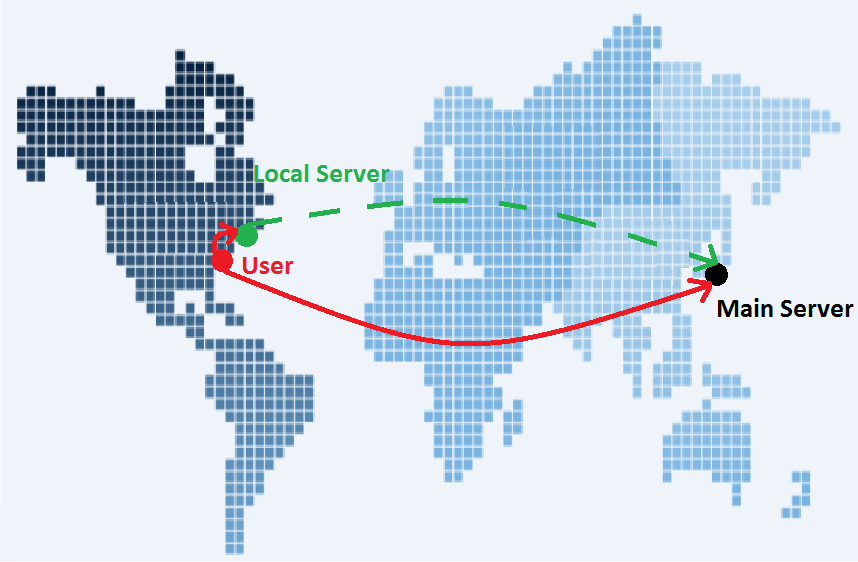
\includegraphics{./images/cdn-map.png}
\caption{The red lines on the map represent the required distances
traveled by requests from a server to the user. Using CDN allows a user
to request static resources from a much closer local server, improving
download times.}
\end{figure}

Because of the reduced wait time for requests and reduced load on your
application server, a CDN is a great option to improve your portal's
performance. Using a CDN with Liferay DXP, however, has some
restrictions.

\subsection{Liferay CDN Requirements}\label{liferay-cdn-requirements}

Liferay DXP only works with CDNs that can dynamically retrieve requested
resources from Liferay DXP. Dynamic resources are resources which change
over time or via interaction with end users and thus cannot be cached.
For this reason, you should check with your CDN provider to make sure
you don't have to manually upload anything in order for the CDN to work.
The CDN must automatically fetch the content from Liferay DXP.

A Liferay DXP-compatible CDN must work like a transparent proxy: A
request first goes to the CDN. If the CDN doesn't have the requested
resource, the CDN makes an identical request back to the origin (Liferay
DXP), caches the resource, then serves the resource.

Once you've configured Liferay DXP to use a CDN (see below), the CDN not
only serves portal resources but also plugin resources (e.g., theme
resources or JavaScript files referenced from a plugin's
\texttt{liferay-portlet.xml} file). The CDN only serves resources that
are actually included in a plugin. It does not serve resources that are
dynamically loaded from external sources.

To get the CDN URL for a resource, developers can simply replace the
portal host in the resource path with
\texttt{themeDisplay.getCDNDynamicResourcesHost()}. Developers should
prefix resources with the CDN host name. They should not manually upload
any resources to the CDN or put anything on the CDN which requires
permission checking or complex policy access.

There are several properties in Liferay DXP that enable you to configure
your CDN and tweak it to suite your portal's needs. You'll learn how to
do this next.

\subsection{Configuring Liferay DXP to Use a
CDN}\label{configuring-liferay-dxp-to-use-a-cdn}

Now that you have a general understanding of what a CDN accomplishes and
how it's used in Liferay DXP, it's time to set one up for yourself. You
can set your CDN and its properties using two different methods:

\begin{enumerate}
\def\labelenumi{\arabic{enumi}.}
\tightlist
\item
  By editing your portal properties file
\item
  By using the Control Panel
\end{enumerate}

To configure your CDN via properties file, you need to create a
\texttt{portal-ext.properties} file in your Liferay Home directory and
set the appropriate CDN properties. You can view the CDN properties and
their descriptions by visiting the
\href{@platform-ref@/7.0-latest/propertiesdoc/portal.properties.html\#Content\%20Delivery\%20Network}{Content
Delivery Network} section of the \texttt{portal.properties} HTML
document.

Once you configure your CDN host, Liferay DXP generates URLs to the
static assets that replace the old host with your new CDN host and so
they are automatically cached and served afterwards by the CDN.

To configure your CDN in the Control Panel, navigate to \emph{Control
Panel} → \emph{Configuration} → \emph{Instance Settings}. In the main
configuration, you'll notice three fields related to CDNs:

\begin{itemize}
\tightlist
\item
  \emph{CDN Host HTTP}
\item
  \emph{CDN Host HTTPS}
\item
  \emph{CDN Dynamic Resources Enabled}
\end{itemize}

\begin{figure}
\centering
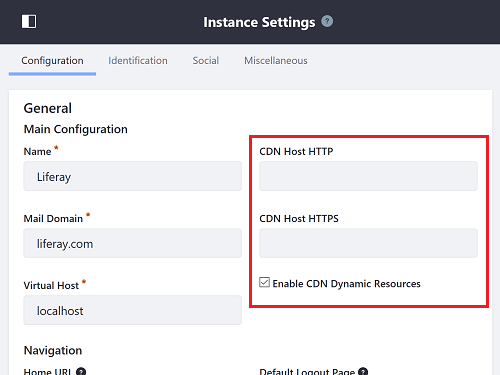
\includegraphics{./images/cdn-control-panel.png}
\caption{The Control Panel lets you configure your portal's CDN.}
\end{figure}

These properties are exactly the same as the ones you can specify in
your \texttt{portal-ext.properties}. Make sure to visit the CDN section
of the Properties Document referenced previously if you don't know how
to fill in the CDN fields. Make sure to specify your CDN host(s) with a
URL that includes the protocol and domain.

Examples,

\emph{CDN Host HTTP:} \texttt{http://cdnhost1.liferay.com}\\
\emph{CDN Host HTTP:} \texttt{https://cdnhost2.liferay.com}

Once you're finished, click \emph{Save} and your old host is replaced
with your new CDN host for static content.

As you can see, configuring a CDN is extremely easy, and can drastically
reduce latency time and improve your portal's performance.

\chapter{Liferay DXP Security}\label{liferay-dxp-security}

Liferay takes security very seriously. Liferay has established several
procedures to make sure that Liferay DXP is as secure as possible. First
of all, Liferay DXP is an open source product. As such, Liferay
encourages security-minded community members to verify the product
they're using. All Liferay users benefit when even a few don't blindly
trust the provider! Please read
\href{https://liferay.com/security}{Liferay security statement} for more
information.

Although we act on community reports, we understands that community
reports alone are not enough. Liferay's internal security team also
works on improving security. Liferay's internal security team conducts
internal security reviews. They check Liferay's source code for common
vulnerabilities that can be accidentally introduced by developers.
Additionally, all Liferay DXP security related code is reviewed by
Liferay's application security team before it's committed. For every
major portal release, Liferay works with external security partners to
perform security scans and penetration testing.

Because the security cycle never ends, the internal application security
team gathers reports from Liferay customers and the Liferay community.
The team also monitors other channels (Twitter, the full disclosure
mailing list, the liferay.com forums, etc.) to catch every security
issue as soon as possible. Once fixed, Liferay's Support, Release, and
other teams work on backporting and releasing security patches for all
supported versions.

\section{Liferay DXP Security
Overview}\label{liferay-dxp-security-overview}

Liferay follows the OWASP Top 10 (2013) and CWE/SANS Top 25 lists to
ensure that Liferay DXP is as secure as possible. Following these
recommendations protects the portal against known kinds of attacks and
security vulnerabilities. For example, Liferay DXP's persistence layer
is generated and maintained by the Service Builder framework which
prevents SQL Injection using Hibernate and parameter based queries.

To prevent Cross Site Scripting (XSS), user-submitted values are escaped
on output. To support integration features, Liferay DXP doesn't encode
input. Data is stored in the original form as submitted by the user.
Liferay DXP includes built-in protection against CSRF attacks, Local
File Inclusion, Open Redirects, Uploading and serving files of dangerous
types, Content Sniffing, Clickjacking, Path Traversal, and many other
common attacks.

To stay on top, Liferay DXP also contains fixes for state-of-the-art
attacks and techniques to improve product security. For example, Liferay
DXP uses PBKDF2 to store passwords. Liferay DXP also contains mitigation
for Quadratic Blowup XXE attack, Rosetta Flash vulnerability, Reflected
File Download, and other kinds of attacks.

\subsection{Authentication Overview}\label{authentication-overview}

Liferay DXP user authentication can take place using any of a variety of
prepared solutions:

\begin{itemize}
\tightlist
\item
  Form authentication using the Sign In Portlet with extensible adapters
  for checking and storing credentials (portal database, LDAP)
\item
  Single-Sign-On (SSO) solutions - NTLM, CAS, SiteMinder, OpenSSO,
  OpenID, Facebook
\item
  SAML plugin
  (\url{https://www.liferay.com/marketplace/-/mp/application/15188711})
\item
  JAAS integration with application server
\end{itemize}

Note: Although Liferay's SSO solutions are incompatible with WebDAV,
they can be used in conjunction with Liferay Sync. See the
\href{/docs/7-0/user/-/knowledge_base/u/publishing-files}{Publishing
Files} article for more information on WebDAV and Liferay Sync.

Remote application authentication and authorization can be done using
the \texttt{AuthVerifier} layer:

\begin{itemize}
\tightlist
\item
  Password based HTTP Basic + Digest authentication
\item
  Token based OAuth plugin
\item
  Portal session based solution for JavaScript applications
\end{itemize}

Both user authentication and remote application authentication are
extensible in Liferay DXP. Developers can create custom Login portlets
and plugins, extend the default Login portlet \texttt{auth.pipeline},
create \texttt{AutoLogin} extensions for SSO, or create custom
\texttt{AuthVerifier} implementations.

\subsection{Authorization and Permission
Checking}\label{authorization-and-permission-checking}

There are several adjustable authorization layers in place to prevent
unauthorized or unsecured access to data:

\begin{itemize}
\tightlist
\item
  Remote IP and HTTPS transport check to limit access to Liferay DXP's
  Java servlets
\item
  Extensible Access Control Policies layer to perform any portal service
  related authorization check
\item
  Extensible role-based permission framework for almost any portal
  entity or data (stored in the portal database or elsewhere)
\item
  Portlet Container security checks to control portlet access
\item
  Remote IP check for portal remote API authentication methods
\item
  Service Access Policies to control access to portal remote API
\end{itemize}

\subsection{Additional Security
Features}\label{additional-security-features}

Liferay DXP supports other features, too. Liferay DXP users can be
assigned to sites, teams, user groups, or organizations. Custom roles
can be created, permissions can be assigned to those roles, and those
roles can be applied to users. Roles are scoped to apply only with a
specific context like a site, an organization, or globally. See Liferay
DXP's \href{}{Roles and Permissions (not yet written)} documentation for
more information.

\noindent\hrulefill

Note: Liferay DXP relies on the application server for sanitizing CRLF
in HTTP headers. You should, therefore, make sure this is properly
configured in your application server, or you may experience false
positives in reports from automatic security verification software such
as Veracode. There is one exception to this for Resin, which does not
have support for this feature. In this case, Liferay DXP sanitizes HTTP
headers.

\noindent\hrulefill

There are additional security plugins available from
\href{https://www.liferay.com/marketplace}{Liferay Marketplace}. For
example, you can find an Audit plugin for tracking user actions or an
AntiSamy plugin for clearing HTML from XSS vectors.

Liferay DXP provides plenty of configuration options that allow its
various security features to be fine-tuned or disabled. Here are a few
examples of these kinds of configuration actions:

\begin{itemize}
\tightlist
\item
  Disable the Sign In portlet's \emph{Create Account} link
\item
  Configure Liferay DXP's HTTPS web server address
\item
  Configure the list of allowed servers to which users can be redirected
\item
  Configure the list of portlets that can be accessed from any page
\item
  Configure the file types allowed to be uploaded and downloaded
\item
  Many other options
\end{itemize}

\subsection{Secure Development
Recommendations}\label{secure-development-recommendations}

Liferay DXP also provides tools to fight vulnerabilities in code.

For secure development, it's important to have security-mined colleagues
in your team. These individuals should consider the security aspects of
each stage of the product lifecycle. It's important to start a
discussion about security early in the project-planning stage so that
threats to user privacy, data, and the system can be identified.

Later, during the implementation phase, developers can use the following
list of APIs to address some of the most common vulnerabilities. These
APIs should be used consistently across Liferay DXP.

Before releasing a product, it's important to ``hack yourself first''.
I.e., you should conduct penetration tests or source code reviews to
catch the low-hanging security-flavored fruit. External penetration
testing is also an option for many companies. It's becoming a more
popular and less expensive service.

Here's short list of Liferay DXP security APIs:

\begin{itemize}
\tightlist
\item
  \texttt{HtmlUtil} - to prevent XSS
\item
  \texttt{HtmlUtil\#escapeXPath} - prevent XPath injection
\item
  \texttt{AuthTokenUtil\#checkCSRFToken} - check CSRF tokens
\item
  \texttt{FileUtil\#createTempFile*} - prevent file system related
  issues
\item
  \texttt{PortalUtil\#escapeRedirect} - prevent open redirects
\item
  \texttt{StringUtil\#random*} - insecure but random enough strings
\item
  \texttt{PwdGenerator\#getPassword}, \texttt{SecureRandomUtil} --
  cryptographically strong pseudorandom output, optimized for
  performance
\item
  \texttt{PasswordEncryptorUtil} - verification and creation of strong
  password hashes, configured to use PBKDF2 by default
\item
  \texttt{DigesterUtil} - SHA-1 hashes, nowadays usable at most for file
  checksums
\end{itemize}

\subsection{Secure Configuration and Run
Recommendations}\label{secure-configuration-and-run-recommendations}

Liferay DXP is built using the ``secure by default'' concept in mind.
Thus, Liferay DXP's default configuration is already very secure. It's
not recommended to disable built-in protections or to allow all values
in security white-lists. Such acts may lead to security misconfiguration
and an insecure Liferay DXP deployment.

For more information about securing a Liferay DXP installation, please
see \url{https://liferay.com/security} and
\url{https://portal.liferay.dev/people/community-security-team} and the
resources listed on those pages.

Also, Liferay DXP customers are advised to deploy security patches as
described on the customer portal:
\url{https://www.liferay.com/group/customer/products/portal/security-vulnerability}

For community and CE deployments, the only way to stay secure is to use
always the latest community version, which contains all previous
security patches. Until a new version is released, the Community
Security Team issues patches for the latest CE version via the
\url{https://portal.liferay.dev/people/community-security-team} page.

\chapter{What is SAML?}\label{what-is-saml}

Liferay DXP's SAML (Security Assertion Markup Language) adapter lets you
execute Single Sign On (SSO) and Single Log Off (SLO) in your
deployment. Each Liferay DXP instance serves as either the Service
Provider (SP) or the Identity Provider (IdP). This article provides the
conceptual framework for Liferay DXP's SSO solution.

\begin{itemize}
\tightlist
\item
  Single Sign On

  \begin{itemize}
  \tightlist
  \item
    Identity Provider initiated SSO
  \item
    Service Provider initiated SSO
  \end{itemize}
\item
  Single Log Off

  \begin{itemize}
  \tightlist
  \item
    Identity Provider initiated SLO
  \item
    Service Provider initiated SLO
  \end{itemize}
\end{itemize}

\noindent\hrulefill

\textbf{Note:} A single Liferay DXP instance is \emph{either} the SP or
the IdP in your SSO setup; it can't be both. You can, however, use
separate instances for both purposes (for example, one instance is the
SP and another is the IdP).

\noindent\hrulefill

Below is background on how SAML works. To jump right to its
configuration, see the articles on
\href{/docs/7-0/deploy/-/knowledge_base/d/setting-up-liferay-as-a-saml-identity-provider}{Setting
Up SAML as an Identity Provider} or
\href{/docs/7-0/deploy/-/knowledge_base/d/setting-up-liferay-as-a-saml-service-provider}{Setting
Up SAML as a Service Provider} for instructions on using the
\href{https://web.liferay.com/marketplace/-/mp/application/15188711}{SAML
adapter}. Use the instructions to make the conceptual magic from this
article come to life!

\noindent\hrulefill

\textbf{Note:} If you're migrating from a Liferay SAML adapter prior to
version 3.1.0, your properties are automatically migrated to settings.
Please see the
\href{/docs/7-0/deploy/-/knowledge_base/d/configuring-saml}{Configuring
SAML} article for details on settings.

\noindent\hrulefill

\section{Important SAML URLs}\label{important-saml-urls}

For reference, here are a few important SAML URLs.

This URL is the default location of Liferay DXP's metadata XML file:

\begin{verbatim}
[host]:[port]/c/portal/saml/metadata
\end{verbatim}

Note that when configuring SAML for Liferay DXP, no importing of SAML
certificates is required. Liferay DXP reads certificates from the SAML
metadata XML file. If you want a third-party application like Salesforce
to read a Liferay SAML certificate, you can export the Liferay DXP
certificate from the keystore. The default keystore file is
\texttt{{[}Liferay\ Home{]}/data/keystore.jks}. The exported certificate
can be imported by a third-party application like Salesforce.

\section{Single Sign On}\label{single-sign-on}

Both the IdP and the SP can initiate the Single Sign On process, and the
SSO flow is different depending on each one. Regardless of how it's
initiated, SSO is configured for HTTPS between the SP and IdP, so all
transport-level communication is encrypted. SAML requests are signed
using certificates configured in Liferay DXP, using the SAML Web Browser
SSO profile as defined in the
\href{http://saml.xml.org/saml-specifications}{SAML 2.0 specification}.

Consider IdP initiated SSO first.

\subsection{Identity Provider Initiated
SSO}\label{identity-provider-initiated-sso}

Sometimes a user enters the SSO cycle by sending a request directly from
the browser to the IdP.

\begin{figure}
\centering
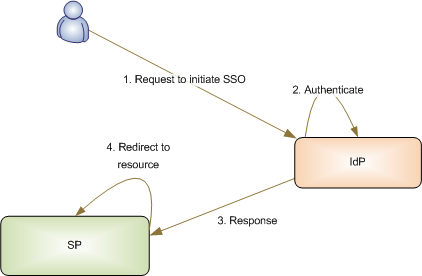
\includegraphics{./images-dxp/saml-idp-initiated-sso.png}
\caption{Identity Provider Initiated SSO}
\end{figure}

\subsection{The SSO Request to the IdP}\label{the-sso-request-to-the-idp}

If Liferay DXP is the IdP, the IdP initiated SSO URL

\begin{itemize}
\tightlist
\item
  Must specify the path as \texttt{/c/portal/saml/sso}.
\item
  Must include the \texttt{entityId} parameter which is the identifier
  to a previously configured Service Provider Connection (SPC).
\item
  May include a \texttt{RelayState} parameter which contains a URL
  encoded value to which the user will be redirected upon successful
  authentication. This URL should point to a location on the desired SPC
  (according to the
  \href{https://docs.oasis-open.org/security/saml/v2.0/saml-bindings-2.0-os.pdf}{SAML
  2.0 standards section 3.4.3}, this value \emph{must not} exceed 80
  bytes in length). It is useful to specify a landing page after SSO has
  been executed.
\end{itemize}

For non-Liferay DXP IdPs (Siteminder, ADFS, etc.), consult the vendor's
documentation on constructing IdP initiated SSO URLs.

If the IdP determines that the user isn't authenticated, it prompts the
user with the appropriate login screen.

\subsection{The SSO Response from the
IdP}\label{the-sso-response-from-the-idp}

Upon successful authentication the IdP constructs a SAML Response. It
includes attribute statements configured in the designated Service
Provider Connection (SPC; see the
\href{/docs/7-0/user/-/knowledge_base/u/setting-up-saml}{next article}
on setting up the SPC in Liferay DXP's SAML adapter).

The IdP sends the response to the Assertion Consumer Service URL using
HTTP-POST or HTTP-Redirect. HTTP-POST is preferred because it reduces
the risk that the URL is too long for a browser to handle. Using
HTTP-POST, the request contains two parameters:

\begin{verbatim}
SAMLResponse
\end{verbatim}

and

\begin{verbatim}
RelayState
\end{verbatim}

\noindent\hrulefill

\textbf{Note:} The method for sending the SAML response (for example,
HTTP-Post) and the Assertion Consumer Service URL are generally imported
as part of the SAML metadata XML provided by the SP. In Liferay DXP, you
import the SP's metadata in the SAML Adapter's Service Provider
Connections tab.

\noindent\hrulefill

\subsection{The SP Processes the SSO
Response}\label{the-sp-processes-the-sso-response}

The SP validates and processes the SAML Response. Liferay DXP's SAML
solution requires \texttt{SAMLResponse} messages to be signed. This
signature process ensures proper identification for the IdP and prevents
potential SAML Response spoofing.

\begin{itemize}
\tightlist
\item
  If one Liferay DXP instance is the IdP and another is the SP, make
  sure the SAML metadata XML file imported into the Liferay DXP SP
  contains the IdP's certificate.
\item
  If Liferay DXP is the IdP and another application is the SP, export
  the certificate from the Liferay DXP IdP and import it into the SP's
  certificate store.
\end{itemize}

If a \texttt{RelayState} is included in the SAML Response, the user is
redirected to it. Otherwise the home page of the SP is served.

\subsection{Service Provider Initiated
SSO}\label{service-provider-initiated-sso}

\begin{figure}
\centering
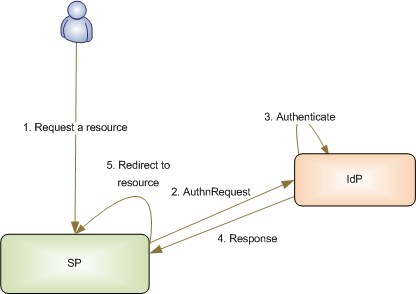
\includegraphics{./images-dxp/saml-sp-initiated-sso.png}
\caption{Service Provider Initiated SSO}
\end{figure}

\subsection{The SSO Request to the SP}\label{the-sso-request-to-the-sp}

When the user's browser requests a protected resource or sign on URL on
the SP, it triggers the SP initiated SSO process. When Liferay DXP is
the SAML SP, SSO is initiated either by requesting
\texttt{/c/portal/login} URL or a protected resource that requires
authentication (for example, a document that is not viewable by the
Guest role). If the user requests a protected resource, its URL is
recorded in the \texttt{RelayState} parameter. If the user requested
\texttt{/c/portal/login}, the \texttt{RelayState} can be set by
providing the \texttt{redirect} parameter. Otherwise, if the
\href{@platform-ref@/7.0-latest/propertiesdoc/portal.properties.html}{portal
property} \texttt{auth.forward.by.last.path} is set to true, the last
accessed path is set as the \texttt{RelayState}. For non-Liferay DXP
SPs, consult the vendor documentation on initiating SSO.

\subsection{The AuthnRequest to the
IdP}\label{the-authnrequest-to-the-idp}

The SP looks up the IdP's Single Sign On service URL and sends an
\texttt{AuthnRequest}. When Liferay DXP is the SP it looks up the
configured SAML Identity Provider Connection and sends a SAML
\texttt{AuthnRequest} to the IdP's Single Sign On service URL as defined
in the SAML metadata XML document. Liferay DXP supports sending and
receiving the \texttt{AuthnRequest} using HTTP-Post or HTTP-Redirect
binding. HTTP-Post is preferred.

If the user doesn't have an active session or if \texttt{ForceAuthn} was
requested by the SP, the user must authenticate by providing his or her
credentials. When Liferay DXP is the IdP, authentication occurs in the
Login Portlet. Liferay DXP decodes and verifies the \texttt{AuthnRequest}
before requesting the user to authenticate.

\subsection{The SSO Response from the
IdP}\label{the-sso-response-from-the-idp-1}

After authentication a SAML Response is constructed, sent to the
Assertion Consumer Service URL of the SP, and verified.

When Liferay DXP is configured as the IdP, any attributes configured on
the Service Provider Connection are included in the response as
attribute statements. The Assertion Consumer Service URL is looked up
from the SAML metadata XML of the SP. The response is sent using
HTTP-Post or HTTP-redirect binding. The IdP automatically makes this
choice based on the SP metadata. HTTP-Post binding is preferred and used
when available. HTTP-Redirect binding is fragile because the signature
and included assertions often make the URL too long for browsers.

When Liferay DXP is configured as the SP, any response and assertion
signatures are verified. Liferay DXP requires the sender to be
authenticated. This is done via whole message signature from the issuing
IdP. Any responses missing the signature are considered unauthenticated
and the response is rejected. The Response can be received via HTTP-Post
binding or HTTP-redirect binding. HTTP-Post binding is preferred for the
reasons mentioned in the previous section. For non-Liferay DXP SP or IdP
vendors, consult their documentation.

The user is redirected to the requested resource or to the URL contained
in the \texttt{RelayState} parameter (for example, the last page the
user accessed before initiating SSO).

\section{Single Log Off}\label{single-log-off}

The Single Log Off request is sent from the user's browser to either the
IdP or to a SP, and the SLO flow differs in each case. First consider
IdP initiated SLO.

\subsection{Identity Provider Initiated
SLO}\label{identity-provider-initiated-slo}

\begin{figure}
\centering
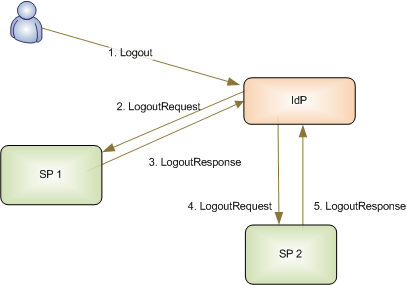
\includegraphics{./images-dxp/saml-idp-initiated-slo.png}
\caption{Identity Provider Initiated SLO}
\end{figure}

\subsection{The SLO Request to the IdP}\label{the-slo-request-to-the-idp}

An IdP initiated SLO request is a SLO request sent directly to the IdP
by the user's browser. When Liferay DXP serves as the IdP, the IdP
initiated SSO URL must specify the URL path as

\texttt{/c/portal/logout}

If the user is signed on to any configured SP, the SAML plugin takes
over the logout process, displaying all the signed on services. The
single logout screen displays the authentication status of each SP and
whether any SPs can't be logged out of (for example, if the SP is down
or doesn't support SLO). For non-Liferay DXP IdPs (Siteminder, ADFS,
etc.) consult the vendor's documentation on constructing IdP initiated
SLO URLs.

The IdP sends a SAML \texttt{LogoutRequest} to the SP.

\begin{itemize}
\tightlist
\item
  When Liferay DXP is configured as the IdP, the \texttt{LogoutRequest}
  is sent using either HTTP-Post, HTTP-Redirect, or SOAP binding.
  HTTP-Post binding is preferred but in its absence, the first available
  SLO endpoint with supported binding is selected.
\item
  When Liferay DXP is configured as the SP, supported bindings for
  \texttt{LogoutRequest} are HTTP-Post, HTTP-Redirect, or SOAP.
\item
  For other IdPs or SPs, please consult the vendor's documentation.
\end{itemize}

\subsection{The SLO Response from the
SP}\label{the-slo-response-from-the-sp}

The SP delivers a \texttt{LogoutResponse} to the IdP. When Liferay DXP
is configured as the SP, the \texttt{LogoutResponse} is delivered using
either HTTP-Post, HTTP-Redirect, or direct response to SOAP request.
HTTP-Post binding is preferred but in its absence, HTTP-Redirect is
used. SOAP is only used to respond to the \texttt{LogoutRequest} over
SOAP binding.

The IdP sends a SAML \texttt{LogoutRequest} to the second SP using
either HTTP-Post, HTTP-Redirect, or SOAP binding.

The second SP then delivers the \texttt{LogoutResponse} to the IdP using
HTTP-Post, HTTP-Redirect, or direct response to SOAP request. The
process is repeated for all SPs the user is logged into. When Liferay
DXP is the IdP, Liferay DXP logs the user out after the last SP has
delivered its \texttt{LogoutResponse} or has timed out.

\subsection{Service Provider Initiated
SLO}\label{service-provider-initiated-slo}

\begin{figure}
\centering
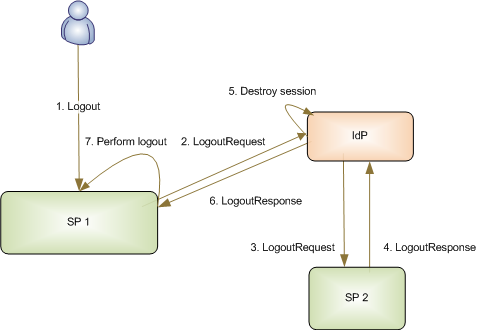
\includegraphics{./images-dxp/saml-sp-initiated-slo.png}
\caption{Service Provider Initiated SLO}
\end{figure}

\subsection{The SLO Request to the SP}\label{the-slo-request-to-the-sp}

In SP initiated SLO, user's browser requests logout directly to the SP.
When Liferay DXP is configured as the SP, the SLO is initiated by
requesting the logout URL

\begin{verbatim}
/c/portal/logout
\end{verbatim}

For other SPs, consult the vendor's documentation on initiating SLO.

A SAML \texttt{LogoutRequest} is sent to the Single Log Out service URL
of the IdP.

\begin{itemize}
\item
  If Liferay DXP serves as the SP, the \texttt{LogoutRequest} is sent to
  the IdP configured by the IdP Connection tab of the SAML provider (see
  the \href{/docs/7-0/user/-/knowledge_base/u/setting-up-saml}{next
  article} to set up the IdP Connection) and the SLO service URL defined
  in the SAML metadata. The request is sent using HTTP-POST or
  HTTP-Redirect binding.
\item
  When Liferay DXP is the IdP, if the user has logged on to other SPs
  the user is presented with a single logout screen with the status of
  each SP logout, flagging any that can't be looged out of (some SPs
  might not support SLO or are currently down). If there are no other
  SPs to log out of, the SAML session terminates and the IdP destroys
  its session.
\end{itemize}

\subsection{The SLO Response from the
SP}\label{the-slo-response-from-the-sp-1}

If the user is logged in to additional SPs (beyond just the initiating
SP), the IdP sends the SAML \texttt{LogoutRequest} to each one. When
Liferay DXP is the IdP, the \texttt{LogoutResponse} is sent using either
HTTP-Post, HTTP-Redirect, or SOAP binding.

Each SP delivers its \texttt{LogoutResponse} to the IdP. When Liferay
DXP is the SP, the \texttt{LogoutResponse} is sent using either
HTTP-Post, HTTP-Redirect or direct response to SOAP request.

After all additional SPs deliver their \texttt{LogoutResponse}s to the
IdP, the IdP destroys its SSO session. When Liferay DXP is the IdP, once
the last SP has delivered its \texttt{LogoutResponse} or has timed out,
the IdP destroys the Liferay DXP session, logging out the user.

Finally, the IdP sends a \texttt{LogoutResponse} to the SP that
initiated SLO. The initiating SP terminates its SAML session and logs
the user out.

\section{Related Topics}\label{related-topics-3}

\begin{itemize}
\tightlist
\item
  \href{/docs/7-0/deploy/-/knowledge_base/d/setting-up-liferay-as-a-saml-identity-provider}{Setting
  Up SAML as an Identity Provider}
\item
  \href{/docs/7-0/deploy/-/knowledge_base/d/setting-up-liferay-as-a-saml-service-provider}{Setting
  Up SAML as a Service Provider}
\item
  \href{/docs/7-0/deploy/-/knowledge_base/d/token-based-single-sign-on-authentication}{Token-Based
  SSO Authentication}
\end{itemize}

\section{Setting up Liferay DXP as a SAML Identity
Provider}\label{setting-up-liferay-dxp-as-a-saml-identity-provider}

An identity provider is a trusted provider that provides single sign-on
for users to access other websites. A service provider is a website that
hosts applications and grants access only to identified users with
proper credentials. SAML is maintained by the
\href{https://www.oasis-open.org/\%20committees/security/}{OASIS
Security Services Technical Committee}. Liferay Portal 6.1 EE and later
versions support SAML 2.0 integration via the
\href{https://web.liferay.com/marketplace/-/mp/application/15188711}{Liferay
SAML 2.0 Provider} application. It is provided from Liferay Marketplace
and allows Liferay DXP to act as a SAML 2.0 identity provider or as a
service provider. \textbf{Important:} You can set Liferay DXP up as an
Identity Provider or as a Service Provider. Each single Liferay DXP
instance can serve as an identity provider or as a service provider, but
\textbf{not both}. Both configurations are covered in this article.

To set Liferay DXP up to act as a SAML Identity Provider, follow the
steps below. Before proceeding, note that in step 3 below, you generate
a keystore for SAML. This keystore has two storage options:

\begin{verbatim}
- In the file system
- In the Documents and Media library
\end{verbatim}

The file system keystore manager is used by default and the default
location is the \texttt{{[}Liferay\ Home{]}/data} directory. To use
Documents and Media library storage for your keystore instead of file
system storage, use the document library keystore manager.

To select a keystore manager, go to \emph{Control Panel} → \emph{System
Settings} → \emph{SAML KeyStoreManager Implementation Configuration}.
There, the options are \emph{Filesystem Keystore Manager} and
\emph{Document Library Keystore Manager}.

The great thing about using Document Library storage is that you can use
any number of
\href{/docs/7-0/deploy/-/knowledge_base/d/document-repository-configuration}{back
end file stores}. These are protected not only by the system in which
you're storing the key, but also by Liferay DXP's permissions system.

Here are the steps for setting up Liferay DXP to act as a SAML Identity
Provider:

\begin{enumerate}
\def\labelenumi{\arabic{enumi}.}
\item
  Install the Liferay SAML 2.0 Provider app. To access the SAML Admin
  interface, click on \emph{Control Panel} → \emph{Configuration} and
  then on \emph{SAML Admin}.
\item
  To begin configuring Liferay DXP to use SAML, select a SAML role for
  Liferay DXP and choose an entity ID.

  \begin{figure}
  \centering
  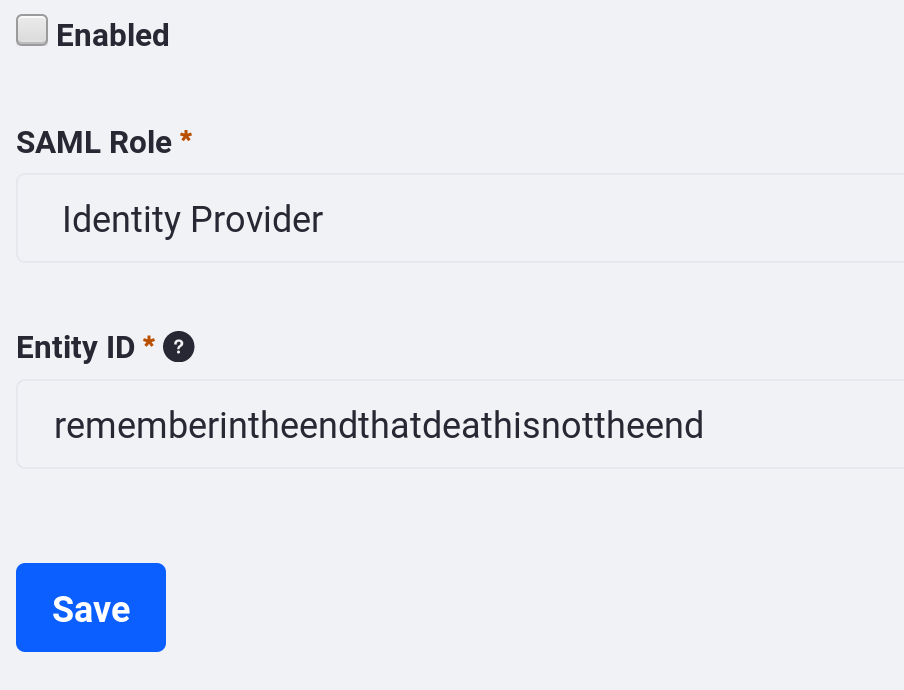
\includegraphics{./images-dxp/saml-initial-config.png}
  \caption{Select a SAML role for Liferay and enter an entity ID.}
  \end{figure}

  Select the \emph{Identity Provider} SAML role. Enter
  \emph{liferaysamlidp} if you're setting up an example Liferay DXP
  instance. Alternatively, choose your own entity ID. Then click
  \emph{Save}. A new Certificate and Private Key section appears.
\item
  The Certificate and Private Key section lets you create a keystore for
  SAML. Click on \emph{Create Certificate} and enter the following
  information:

  \begin{itemize}
  \tightlist
  \item
    Your common name (your first and last name)
  \item
    The name of your organization
  \item
    The name of your organizational unit
  \item
    The name of your city or locality
  \item
    The name of your state or province
  \item
    The name of your country
  \item
    The length in days that your keystore will remain valid (how long
    before the keystore expires)
  \item
    The key algorithm (RSA is the default)
  \item
    The key length in bits (2048 is the default)
  \item
    The key password
  \end{itemize}

  When you enter all the required information, click \emph{Save}.

  When you create the certificate and private key, you also create a
  keystore if one doesn't already exist. As described above, this
  keystore has two storage options: file system storage (the default)
  and Documents and Media storage.
\item
  After you click \emph{Save}, you can click \emph{Replace Certificate}
  at any time to replace the current certificate with a new one if your
  old one has expired or if you want to change the key's password.

  \begin{figure}
  \centering
  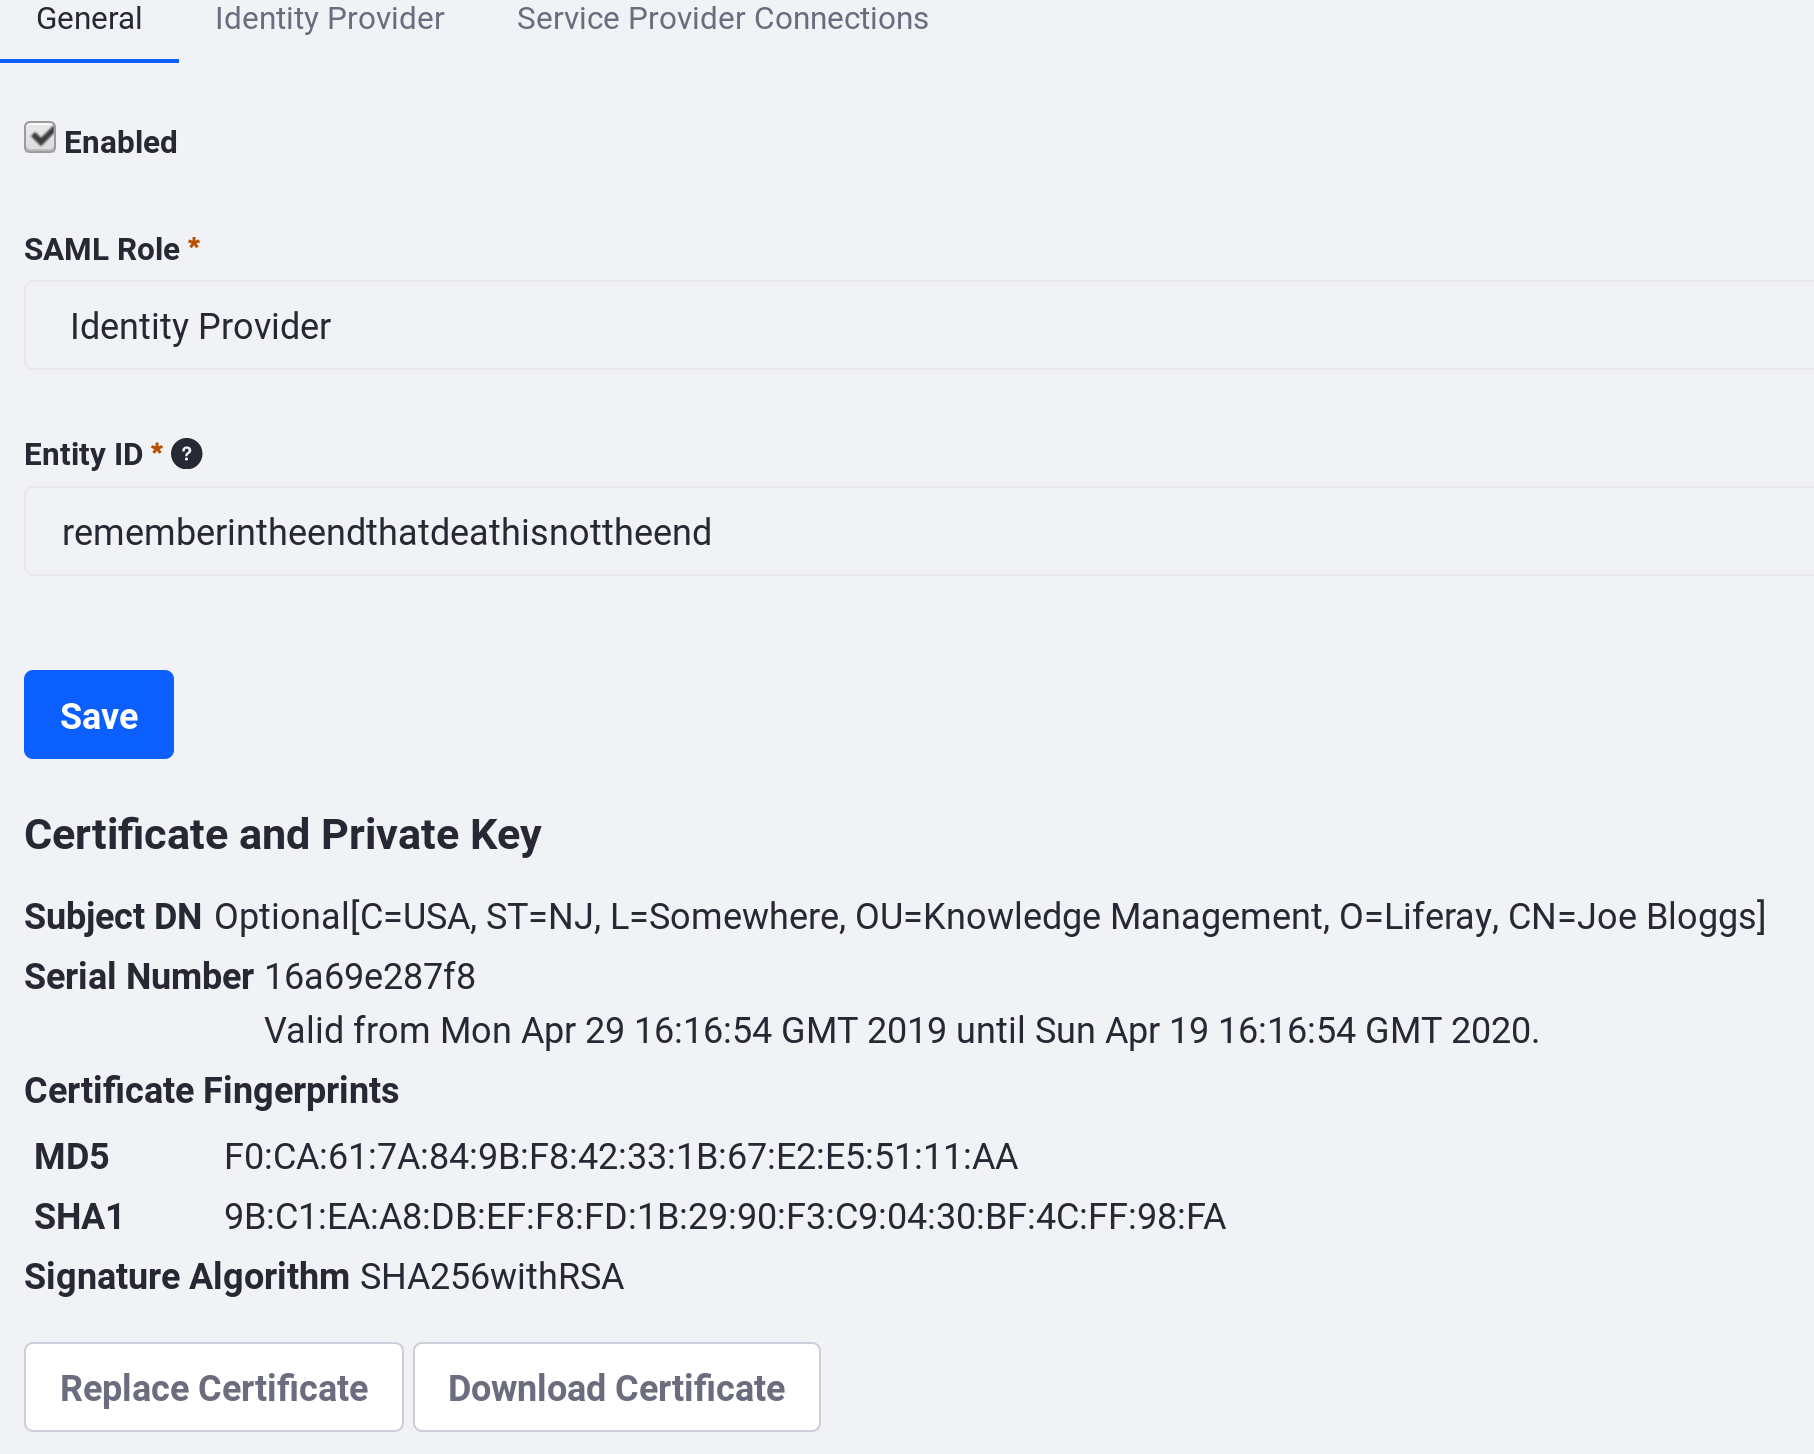
\includegraphics{./images-dxp/saml-keystore-info.png}
  \caption{The General tab of the SAML Admin portlet displays
  information about the current certificate and private key and allows
  administrators to download the certificate or replace the
  certificate.}
  \end{figure}

  Three more tabs now appear:

  \begin{itemize}
  \item
    \emph{General}: This tab lets you enable or disable a SAML IdP and
    lets you manage the required keystore.
  \item
    \emph{Identity Provider}: This tab contains other required
    configurations such as whether to enable SSL. If SSL has been
    enabled, then SAML requests are not approved unless they are also
    encrypted.
  \item
    \emph{Service Provider Connections}: This tab manages any Service
    Providers connected to this Liferay DXP instance.

    See below for more information on the Identity Provider and Service
    Provider Connections tabs.
  \end{itemize}
\item
  After you save your certificate and private key information, check the
  \emph{Enabled} box at the top of the General tab and click
  \emph{Save}. You successfully set Liferay DXP up as a SAML Identity
  Provider!
\end{enumerate}

\subsection{Changing the Identity Provider
Settings}\label{changing-the-identity-provider-settings}

To configure Liferay DXP's SAML Identity Provider Settings, navigate to
the \emph{Identity Provider} tab of the SAML Admin Control Panel entry.

The \emph{Identity Provider} tab includes these options:

\textbf{Sign Metadata?:} When this box is checked, the metadata XML file
that's produced is signed.

\textbf{SSL Required:} When this box is checked, any SAML messages that
are \emph{not} sent over SSL are rejected. This affects URLs in the
generated metadata.

\textbf{Require Authn Request Signature?:} When this box is checked,
each Authn Request must be signed by the sending Service Provider. In
most cases, this should be enabled.

\textbf{Session Maximum Age:} Specify the maximum duration of the SAML
SSO session in seconds. If this property is not set or is set to
\texttt{0}, the SSO session has an unlimited duration. The SSO session
maximum duration can be longer than the portal session maximum duration.
If the portal session expires before the SSO session expires, the user
is logged back in to Liferay DXP automatically. SSO session expiration
does not trigger a single logout from all service providers. You can use
the session maximum age, for example, to force users to sign in again
after a certain period of time.

\textbf{Session Timeout:} Specify the maximum idle time of the SAML SSO
session. Even if the session maximum age is unlimited, the SSO session
expires whenever the user's idle time reaches the limit set by the
session timeout property.

\subsection{Checkpoint}\label{checkpoint}

Before adding a Service Provider (SP), verify you've completed these
tasks:

\begin{enumerate}
\def\labelenumi{\arabic{enumi}.}
\item
  A SAML keystore has been generated. It can be stored in one of two
  locations: the \texttt{data} folder or in the Documents and Media
  library.
\item
  On the \emph{Identity Provider} tab, the following settings have been
  set:

  \begin{enumerate}
  \def\labelenumii{\alph{enumii}.}
  \item
    \textbf{Sign Metadata} has been checked.
  \item
    \textbf{SSL Required} - checked if SSL is active elsewhere. SSL is
    disabled by default.
  \item
    \textbf{Authn Request Signature Required:} has been checked.
  \item
    \textbf{Session Maximum Age:} has been set. If set to \texttt{0},
    then the SSO has an unlimited duration.
  \item
    \textbf{Session Timeout:} Specify the maximum idle time of the SAML
    SSO session.
  \end{enumerate}
\item
  Once the \emph{Enabled} checkbox has been checked, the IdP is now
  live, and you can generate the required metadata. This URL is the
  default location of Liferay DXP's metadata XML file:

\begin{verbatim}
 [host]:[port]/c/portal/saml/metadata 
\end{verbatim}
\end{enumerate}

If this URL does not display correctly, then the SAML instance has not
been enabled. Use the URL or click \emph{Save} in the browser to
generate an actual \texttt{XML} file.

\subsection{Adding a SAML Service
Provider}\label{adding-a-saml-service-provider}

Of course, setting up Liferay DXP as a SAML Identity Provider is only
useful if you can connect to one or more SAML Service Providers.
Navigate to the Service Provider Connections tab of the SAML Admin
Control Panel entry and click the \emph{Add Service Provider} button to
add a SAML Service Provider.

The New Service Provider page includes these options:

\textbf{Name:} The name of the Service Provider with which to connect.
The name can be anything; it's purely cosmetic.

\textbf{Entity ID:} The Service Provider's entity ID. This value must
match the entity ID declared in the Service Provider metadata.

\textbf{Enabled:} When this box is checked, the Service Provider
connection is active.

\textbf{Assertion Lifetime:} Defines the number of seconds after which
the SAML assertion issued by the Identity Provider should be considered
expired.

\textbf{Metadata:} You can either provide a URL to the Service Provider
metadata XML file or you can manually upload the Service Provider
metadata XML file. If you provide a URL, the XML file is automatically
retrieved and periodically polled for updates. The update interval can
be configured in System Settings with the
\texttt{saml.metadata.refresh.interval} property which specifies a
number of seconds. If fetching the metadata XML file by URL fails, you
can't enable the Service Provider connection. If the Identity Provider
server cannot access the metadata via URL, you can upload the XML file
manually. In this case, the metadata XML file is not updated
automatically.

\textbf{Name Identifier Format:} Choose the Name Identifier Format used
in the SAML Response. This should be set according to what the Service
Provider expects to receive. For Liferay Service Providers, any
selection other than email address indicates that the Name Identifier
refers to screen name. The formats don't have any special meaning to
Liferay Identity Providers. The NameID value is defined by the Name
Identifier attribute. See the next option.

\textbf{Name Identifier Attribute Name:} This specifies which attribute
of the Liferay DXP \texttt{User} object to use as the NameID value.
Possible values include \texttt{emailAddress}, \texttt{screenName} and
\texttt{uuid}. Additionally, you can prefix the name with
\texttt{static:} or \texttt{expando:}. If you use the prefix
\texttt{static}, the value is whatever comes after \texttt{static:}. If
you use the prefix \texttt{expando}, the value is whatever custom field
is specified after \texttt{expando:}. For example, \texttt{expando:SSN}
would look up the \texttt{User} custom field with the name \texttt{SSN}.

\textbf{Attributes Enabled:} Include and resolve assertion attributes.

\textbf{Attributes Namespace Enabled:} When this box is checked, the
attribute names are namespaced like this:

\begin{verbatim}
urn:liferay:user:expando:
urn:liferay:user:
urn:liferay:groups:
urn:liferay:organizationRole:
urn:liferay:organization:
urn:liferay:roles:
urn:liferay:siteRole:
urn:liferay:userGroupRole:
urn:liferay:userGroups:
\end{verbatim}

\textbf{Attributes:} Enter a list of attributes to include in the
assertion, one per line. Each line is an expression that gets parsed.
Examples:

\begin{verbatim}
organizations
organizationRoles
roles
siteRoles
userGroups
static:[attributeName]=[attributeValue]
expando:[userCustomFieldName] 
\end{verbatim}

Note that the full namespace depends on the attribute name. Attribute
namespaces can be very useful. Use them when attribute names from
different namespaces might conflict. For example, \texttt{expando:user}
vs \texttt{urn:liferay:roles:user}.

\textbf{Keep Alive URL:} If users are logged into several Liferay DXP SP
instances via a Liferay DXP IdP, their sessions can be kept alive as
long as they keep a browser window open to one of them. Configure this
only if the SP is Liferay DXP. The URL is
\texttt{https://{[}SP\ host\ name{]}/c/portal/saml/keep\_alive}.

\subsection{Checkpoint}\label{checkpoint-1}

Verify your settings are correct when connecting the Liferay DXP-based
IdP to its first SP. SPs connect to only one IdP, so if the first one
doesn't work, the rest won't either.

\begin{enumerate}
\def\labelenumi{\arabic{enumi}.}
\item
  Provide a general name for the SP.
\item
  The \texttt{Entity\ ID} name must be identical to the one declared in
  the Service Provider metadata.
\item
  Check the \emph{Enabled} checkbox.
\item
  Set a value for the \emph{Assertion Lifetime}.
\item
  Make sure the SP's metadata has been provided either as a URL or an
  XML file has been uploaded.
\item
  Make sure \emph{Name Identifier Format} and \emph{Name Identifier
  Attribute Name} have been set.
\item
  Make sure \emph{Attributes Namespace Enabled} has been set.
\end{enumerate}

If you don't have a Service Provider to add right now, that's fine. In
the next section, you'll learn how to set Liferay DXP up as a SAML
Service Provider. After you set up another Liferay DXP instance as a
Service Provider, come back to this Liferay DXP installation and add the
Service Provider: \emph{Control Panel} → \emph{SAML Admin} →
\emph{Service Provider Connections} → \emph{Add Service Provider}.

\section{Setting up Liferay DXP as a SAML Service
Provider}\label{setting-up-liferay-dxp-as-a-saml-service-provider}

Many of these steps are similar to configuring Liferay DXP as a SAML
Identity Provider. As a reminder, a single Liferay DXP installation can
be configured as a SAML Identify Provider \emph{or} as a SAML Service
Provider but not as both. If you already set up one Liferay DXP
installation as a SAML Identity Provider, use a \emph{different} Liferay
DXP installation as a SAML Service Provider.

\noindent\hrulefill

\textbf{Note:} If you're using a third party IdP with Liferay DXP as the
SP, all messages coming from the IdP must be signed. If they're not, an
error message appears and communication between the IdP and Liferay DXP
fails.

\noindent\hrulefill

\begin{enumerate}
\def\labelenumi{\arabic{enumi}.}
\item
  Install the Liferay SAML 2.0 Provider app. To confirm that the app was
  successfully deployed, look for the \emph{SAML Admin} entry in the
  Configuration section of the Control Panel.
\item
  To begin configuring Liferay DXP to use SAML, you must select a SAML
  role for Liferay DXP and you need to choose an entity ID. Select the
  \emph{Service Provider} SAML role. Enter \emph{liferaysamlsp} if
  you're setting up an example Liferay DXP installation. Alternatively,
  choose your own entity ID. Then click \emph{Save} and a new section
  entitled Certificate and Private Key appears.
\item
  The Certificate and Private Key section is for creating a keystore for
  SAML. Click \emph{Create Certificate} and enter the following
  information:

  \begin{itemize}
  \tightlist
  \item
    Your common name (your first and last name)
  \item
    The name of your organization
  \item
    The name of your organizational unit
  \item
    The name of your city or locality
  \item
    The name of your state or province
  \item
    The name of your country
  \item
    The length in days that your keystore will remain valid (how long
    before the keystore expires)
  \item
    The key algorithm (RSA is the default)
  \item
    The key length in bits (2048 is the default)
  \item
    The key password
  \end{itemize}

  When you enter all the required information, click \emph{Save}.
\item
  After you clicked \emph{Save}, check that you can view information
  about your certificate or download your certificate. If you can, you
  successfully created a keystore. After you create a keystore,
  additional options appear. There are three tabs:

  \begin{itemize}
  \item
    \emph{General}: This tab enables or disables SAML IdP and manages
    the required keystore.
  \item
    \emph{Service Provider}: This tab manages basic and advanced
    configurations for the SP.
  \item
    \emph{Identity Provider Connection}: This tab manages connections to
    the IdP. There can be only one IdP connection.
  \end{itemize}

  Note that these options are different than if you were setting up
  Liferay DXP as an Identity Provider.
\item
  Next, you need to configure an Identity Provider connection. Click on
  the \emph{Identity Provider Connection} tab. Enter a name for the
  Identity Provider, enter its entity ID, and enter its metadata URL. If
  you have already followed the previous instructions and configured a
  separate Liferay DXP installation as an Identify provider, you'd enter
  the following information:

  \begin{itemize}
  \tightlist
  \item
    Name: \emph{Liferay IdP}
  \item
    Entity ID: \emph{liferaysamlidp}
  \item
    Clock Skew
  \item
    Force Authn
  \item
    Metadata URL: http://localhost:8080/c/portal/saml/metadata (test
    this URL first)
  \item
    Name Identifier Format
  \item
    Attribute Mapping
  \item
    Keep Alive URL
  \end{itemize}

  \textbf{Important}: The Liferay SAML 2.0 Provider app supports using
  \emph{either} a URL to a SAML IdP metadata file \emph{or} an actual
  (uploaded) SAML metadata XML file. The value entered in the
  \emph{Metadata URL} field will only be persisted to the database when
  there is one entered metadata URL and there is no specified metadata
  XML file. Otherwise, Liferay DXP keeps the original metadata URL in
  the database. This behavior ensures that once a metadata URL has been
  specified, there will always be a metadata URL saved in the database.
  This way, if a portal administrator forgets the previously entered
  metadata URL or its format, he or she can simply look at the displayed
  metadata URL and either choose to modify the displayed metadata URL or
  to overwrite the previously saved metadata URL by specifying a
  metadata XML file.

  Currently, the SAML Provider app does not provide a way to ``clear''
  the SAML IdP metadata URL or metadata XML file fields using the
  Control Panel UI. If you really need to clear these fields, it's
  possible (but not recommended) to delete the contents of the SAML IdP
  metadata URL and metadata XML file columns of the
  \texttt{SamlSpIdpConnection} table of Liferay DXP's database.
\item
  Finally, after you save your certificate and private key information
  and configure an Identity Provider connection, check the
  \emph{Enabled} box at the top of the General tab and click
  \emph{Save}. Liferay DXP is now a SAML Service Provider!
\end{enumerate}

Note that the SAML Service Provider session is tied to the normal
session on the application server. Session expiration on the application
server terminates the session on the Service Provider but does not
initiate single logout.

\subsection{Checkpoint}\label{checkpoint-2}

\begin{enumerate}
\def\labelenumi{\arabic{enumi}.}
\item
  A SAML keystore has been generated.
\item
  Verify the connection to the IdP.

  \begin{enumerate}
  \def\labelenumii{\alph{enumii}.}
  \item
    \emph{Name}: generic name for the IdP.
  \item
    \emph{Entity ID}: the same name of the IdP. If the IdP is another
    Liferay DXP instance, then it is the same name as the above example.
  \item
    \emph{Metadata URL}: The IdP's metadata as a URL or as an XML file.
  \item
    If the IdP is another Liferay DXP instance, ensure its corresponding
    Service Provider Connection for this SP is enabled.
  \end{enumerate}
\item
  On the \emph{General} tab, the \emph{Enabled} checkbox has been
  checked.
\item
  Once \emph{Enabled} checkbox has been checked, the service provider's
  metadata becomes available:

\begin{verbatim}
 [host]:[port]/c/portal/saml/metadata
\end{verbatim}
\end{enumerate}

\subsection{Changing the SAML Service Provider
Settings}\label{changing-the-saml-service-provider-settings}

If you'd like to configure Liferay DXP's SAML Service Provider Settings,
navigate to the Service Provider tab of the SAML Admin portlet.

The Service Provider tab includes these options:

\textbf{Require Assertion Signature?:} When this box is checked, SAML
assertions must be individually signed in addition to the entire SAML
message.

\noindent\hrulefill

\textbf{Note:} Because Liferay requires the SAML response to be signed,
individual assertions need not be signed. The SP and IdP should always
communicate over \texttt{https} to have encryption at the transport
level.

If you believe man-in-the-middle attacks are possible, the SAML response
can be signed.

\noindent\hrulefill

\textbf{Clock Skew:} Clock skew is a tolerance in milliseconds used by
the Service Provider for verifying expiration of messages and
assertions. This can be used to mitigate time differences between the
clocks of the Identity Provider and the Service Provider. This usually
only matters when assertions have been made to expire very quickly.

\textbf{LDAP Import Enabled:} When this box is checked, user information
is imported from the configured LDAP connection based on the resolved
NameID. LDAP connections can be configured from Instance Settings.

\textbf{Sign Authn Requests:} When this box is checked, the AuthnRequest
is signed even if the Identity Provider metadata indicates that it's not
required.

\textbf{Sign Metadata:} When this box is checked, the metadata XML file
is signed.

\textbf{SSL Required:} When this box is checked, any SAML messages that
are not sent over HTTPS are rejected. This does not affect how URLs are
generated.

\subsection{Changing the SAML Identity Provider Connection
Settings}\label{changing-the-saml-identity-provider-connection-settings}

If you'd like to configure Liferay DXP's SAML Identity Provider
Settings, navigate to the Identity Provider Connection tab of the SAML
Admin portlet.

\textbf{Name:} The name of the Identity Provider with which to connect.

\textbf{Entity ID:} The Identity Provider's entity ID. This value must
match the entity ID declared in the Identity Provider metadata.

\textbf{Clock Skew:} Clock skew is a tolerance in milliseconds used by
the Service Provider for verifying expiration of messages and
assertions. This can be used to mitigate time differences between the
clocks of the Identity Provider and the Service Provider. This usually
only matters when assertions have been made to expire very quickly.

\textbf{Force Authn:} When this box is checked, the Service Provider
asks the Identity Provider to re-authenticate the user before verifying
the user.

\textbf{Metadata:} You can either provide a URL to the Identity Provider
metadata XML file or you can manually upload it. If you provide a URL,
the XML file is automatically retrieved and periodically polled for
updates. You can change the update interval in System Settings by
modifying the \texttt{saml.metadata.refresh.interval} property which
specifies a number of seconds. If fetching the metadata XML file by URL
fails, you can't enable the Identity Provider connection. If the
metadata is inaccessible via URL, you can upload the XML file manually.
In this case, the metadata XML file is not updated automatically.

\textbf{Name Identifier Format:} Choose the Name Identifier Format used
in the SAML Response. This should be set according to what the Service
Provider expects to receive. For Liferay Service Providers, any
selection other than email address indicates that the Name Identifier
refers to screen name. The formats don't have any special meaning to
Liferay Identity Providers. The NameID value is defined by the Name
Identifier attribute.

\textbf{Attribute Mapping:} The attribute mapping is done from the
attribute name or friendly name in the SAML Response to the Liferay DXP
attribute name. For example, if you want to map a response attribute
named \texttt{mail} to the Liferay DXP attribute \texttt{emailAddress},
you'd enter the following mapping:

\begin{verbatim}
mail=emailAddress
\end{verbatim}

Available Liferay DXP attributes are: \texttt{emailAddress},
\texttt{screenName}, \texttt{firstName}, \texttt{lastName},
\texttt{modifiedDate}, and \texttt{uuid}.

\textbf{Keep Alive URL:} If users are logged into several Liferay DXP SP
instances via a Liferay DXP IdP, their sessions can be kept alive as
long as they keep a browser window open to one of them. Configure this
only if the IdP is Liferay DXP. The URL is
\texttt{https://{[}IdP\ host\ name{]}/c/portal/saml/keep\_alive}. On the
Liferay DXP IdP, configure this URL the same way, but point back to this
SP.

Save your changes when you are finished configuring the Liferay DXP
instance as a service provider. There is no need to restart the server
and the changes will be applied immediately.

The previous two sections explained how to use the SAML 2.0 Provider
app's Control Panel interface to configure Liferay DXP as an Identity
Provider or as a Service Provider. Such configurations should only be
made through the SAML Control Panel interface and not via properties.
Some features of the Liferay SAML 2.0 Provider app are not available as
properties.

\noindent\hrulefill

\textbf{Limitation:} The Liferay SAML app can only be used with a single
virtual host. Technically, this means that in the SAML metadata for
Liferay DXP, only one binding can be added in this form:

\begin{verbatim}
 <md:EntityDescriptor>
 ...
 <md:SPSSODescriptor>
 ...
 <md:AssertionConsumerService Binding="urn:oasis:names:tc:SAML:2.0:bindings:HTTP-POST" Location="https://portal.domain.com/c/portal/saml/acs" index="1" isDefault="true" />
 ...
 </md:SPSSODescriptor>
 </md:EntityDescriptor>
\end{verbatim}

\noindent\hrulefill

\subsection{Setting Up Liferay DXP as a SAML Service Provider in a
Clustered
Environment}\label{setting-up-liferay-dxp-as-a-saml-service-provider-in-a-clustered-environment}

If you want to use the Liferay SAML 2.0 Provider app as an SSO solution
for a clustered Liferay DXP environment, follow the steps in this
section. Before proceeding, make sure that the following assumptions
apply to your scenario.

If you're running a multi-node cluster behind a load balancer, follow
these steps to enable all the nodes as SPs.

Before you begin, consider the type of keystore manager you want your
cluster to use.

To select a keystore manager, go to \emph{Control Panel} → \emph{System
Settings} → \emph{SAML KeyStoreManager Implementation Configuration}.
There, the options are \emph{Filesystem Keystore Manager} and
\emph{Document Library Keystore Manager}.

All nodes in the cluster should be configured to use the same Keystore
Manager.

If using the Filesystem Keystore Manager (the default):

\begin{enumerate}
\def\labelenumi{\arabic{enumi}.}
\item
  Configure each node of your
  \href{/docs/7-0/deploy/-/knowledge_base/d/liferay-clustering}{Liferay
  DXP cluster} as a SAML service provider using the instructions of the
  previous section.
\item
  Copy the keystore file
  (\texttt{{[}Liferay\ Home{]}/data/keystore.jks}, by default) from the
  first Liferay DXP node to the remaining Liferay DXP nodes. This file is
  the Java keystore that's created by the SAML Provider app. The
  keystore contains the valid or self-signed certificate managed by the
  SAML Provider app.
\item
  Verify that the service provider metadata has been generated to be
  used either as a URL or an XML file. The metadata is the same for all
  nodes because of the same database back-end. The IdP's request goes
  through the load balancer.
\item
  At this point, all the Liferay DXP nodes have the same SAML SP
  configuration and each of them can respond to web requests and handle
  the SAML protocol. To test your SSO solution, sign into Liferay DXP
  via your load balancer, navigate to a few pages of a few different
  sites, and then log out.
\end{enumerate}

If using the Document Library Keystore Manager, skip step 3 because the
keystore file is stored in the database shared by all the nodes.

Now you know how to configure Liferay DXP either as a SAML identity
provider or a service provider. You also know how to configure SAML in a
clustered environment.

\section{Configuring SAML}\label{configuring-saml}

As noted in the previous tutorials, anything related to configuring SP
connections must be done through the SAML Admin UI where configurations
are saved to Liferay's database. SP connections can no longer be made
via properties files as they were in versions prior to 3.1.0.

This is an portal instance scoped configuration which can be managed via
OSGi Configuration Admin. The affected properties are those in the
\texttt{SAMLProviderConfiguration} metatype:

\begin{verbatim}
- `saml.keystore.credential.password`
- `saml.sp.assertion.signature.required`
- `saml.idp.authn.request.signature.required`
- `saml.sp.clock.skew`
- `saml.default.assertion.lifetime`
- `saml.sp.default.idp.entity.id`
- `saml.enabled`
- `saml.entity.id`
- `saml.sp.ldap.import.enabled`
- `saml.role`
- `saml.idp.session.maximum.age`
- `saml.idp.session.timeout`
- `saml.sp.sign.authn.request`
- `saml.sign.metadata`
- `saml.ssl.required`
- `saml.idp.metadata.name.id.attribute`
\end{verbatim}

The SAML Admin UI remains the place for creating the portal instance
scoped configuration instances.

\noindent\hrulefill

\textbf{Note:} Don't use OSGi \texttt{.config} files or Liferay DXP's
System Settings Control Panel application to configure SAML providers
(IdP or SP). The System Settings UI is auto-generated, and is for
advanced admins. It does not perform the enhanced validation on the
fields that the SAML Admin UI performs, so it could allow administrators
to create invalid configurations.

\noindent\hrulefill

Note that there is also a system wide configuration, represented by the
\texttt{SamlConfiguration} metatype.

If you used Liferay 6.2, please note that the following system wide
properties were removed:

\begin{verbatim}
`saml.metadata.paths` (served no purpose after removal of SP connection defaults)
`saml.runtime.metadata.max.refresh.delay`
`saml.runtime.metadata.min.refresh.delay`
\end{verbatim}

The latter two properties were replaced with the single property
\texttt{saml.runtime.metadata.refresh.interval}.

Note also the introduction of the \emph{SAML KeyStoreManager
Implementation Configuration} in \emph{Control Panel} → \emph{System
Settings}. The options for this configuration are explained above in the
Setting up Liferay DXP as a SAML Identity Provider section.

\section{Logging in to Liferay DXP}\label{logging-in-to-liferay-dxp}

One of the primary functions of a web portal is to restrict access to
different pages, content, and web applications. These kinds of portal
resources should only be accessible by the appropriate users. E.g., a
student who logs in to a university portal should not be able to access
the same resources that are available to a professor. Similarly, a
patient who logs in to a health care portal should not be able to access
the same resources that are available to a doctor. Some portal resources
(at least a login page) should be available to users who have not logged
in. In Liferay DXP, users who have not logged in are called \emph{guest}
users.

Liferay DXP's Sign In portlet provides the basic means for users to log
in to Liferay DXP. By default, users can also use the Sign In portlet to
create new accounts or to request a password reset. The home page of a
default Liferay DXP installation contains a Sign In portlet. You can
access this page at \url{http://localhost:8080/web/guest/home} if you're
running Liferay DXP locally.

\begin{figure}
\centering
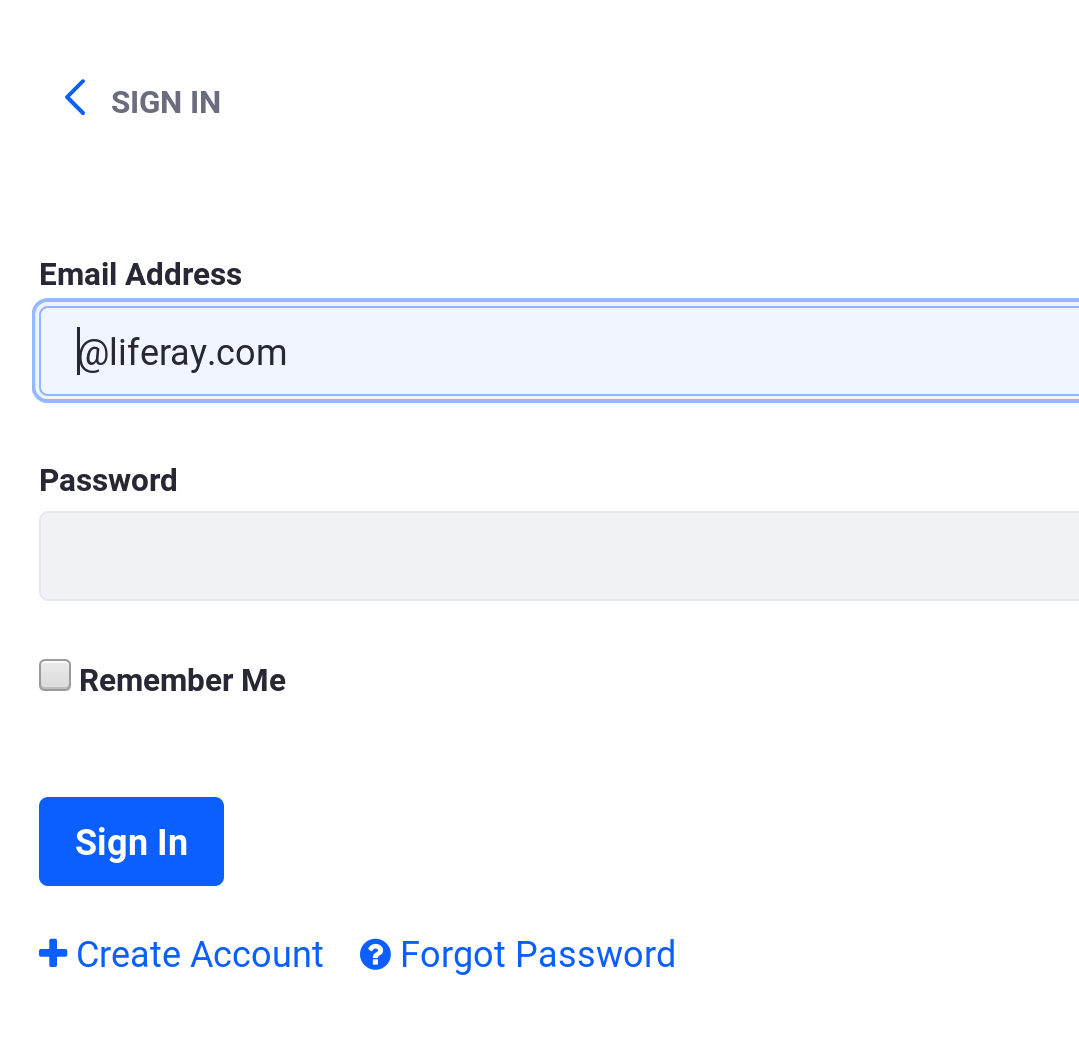
\includegraphics{./images/sign-in-portlet.png}
\caption{By default, the Sign In portlet allows users to log in, create
a new account, or request a password reset.}
\end{figure}

Even if the Sign In portlet has not been added to any Liferay DXP page
that's accessible to a guest user, users can still access it by
navigating to this URL:

\begin{itemize}
\tightlist
\item
  \url{localhost:8080/c/portal/login}
\end{itemize}

Note that Liferay DXP's configured authentication type determines the
type of credentials that the user needs to enter in order to log in.
Liferay DXP supports three authentication types: authentication by email
address, screen name, or user ID. To choose an authentication type,
navigate to the Control Panel, click on \emph{Configuration} →
\emph{Instance Settings} → \emph{Authentication} and use the \emph{How
do users authenticate?} dropdown to make a selection. Alternatively, add
the following lines to your \texttt{portal-ext.properties} file,
uncomment the appropriate line, comment out the others, and restart your
Liferay DXP server.

\begin{verbatim}
company.security.auth.type=emailAddress
#company.security.auth.type=screenName
#company.security.auth.type=userId
\end{verbatim}

Liferay DXP's default authentication type uses users' email addresses.
Users' screen names or user IDs can be used instead. Screen names are
chosen when a new account is created either by the user or by an
administrator. User IDs are autogenerated by Liferay DXP. Regardless of
which authentication type is configured, users must always enter a
password to log in to Liferay DXP.

By default, guest users can create accounts on your portal by clicking
on the \emph{Create Account} link in the Sign In portlet, completing the
form, and submitting it. If a user already has an account but has
forgotten its password, the user can click on the \emph{Forgot Password}
link to request a password reset. Both the \emph{Create Account} form
and the \emph{Forgot Password} form include a CAPTCHA-based text
verification field. Using \href{http://www.captcha.net}{CAPTCHA}
prevents bots from submitting these forms. Liferay DXP can be configured
to use
\href{https://www.google.com/recaptcha/intro/index.html}{reCAPTCHA}
instead of CAPTCHA. One advantage of using reCAPTCHA is that it can
allow visually impaired users to pass the test. To configure Liferay DXP
to use reCAPTCHA, navigate to the Control Panel, then click on
\emph{System} → \emph{Server Administration} → \emph{CAPTCHA}.

The security requirements of some web portals require that all user
accounts be created by administrators. Liferay DXP supports this use
case by allowing the \emph{Create Account} to be removed. To prevent
guest users from creating new user accounts, navigate to the Control
Panel, click on \emph{Configuration} → \emph{Instance Settings} →
\emph{Authentication} and uncheck the \emph{Allow strangers to create
accounts?} box. You can also disallow users from requesting forgotten
passwords or from requesting password reset links by unchecking the
appropriate boxes.

\begin{figure}
\centering
\includegraphics{./images/sign-in-portlet2.png}
\caption{Here's a view of the Sign In portlet with the \emph{Create
Account} and \emph{Forgot Password} options removed.}
\end{figure}

Remember that using the Sign In portlet provides the most basic way for
users to log in to Liferay DXP but it's not the only way. Liferay DXP
allows user accounts to be imported from and exported to LDAP
directories. Liferay DXP can be configured to use single-sign-on (SSO)
solutions. Liferay DXP supports token-based authentication. This
mechanism allows remote web applications to authenticate to Liferay DXP.
Please refer to the other articles in this section for more information.
Finally, remember that Liferay DXP's user authentication and remote
application authentication mechanisms are extensible.

\section{Service Access Policies}\label{service-access-policies}

\emph{Service access policies} are a new feature in 7.0. They are an
additional layer of web service security defining services or service
methods that can be invoked remotely. Many of them can be applied at
once to produce a combined effect. Service access policies apply only to
remote services, not to local services. To help you understand how
service access policies fit into the big picture, here's a summary of
Liferay DXP's web service security layers:

\textbf{IP permission layer:} The IP address from which a web service
invocation request originates must be white-listed in the Liferay DXP
server's portal properties file. Any attempted web service invocation
coming from a non-whitelisted IP address automatically fails.

\textbf{Service access policy layer:} The method corresponding to a web
service invocation request must be whitelisted by each service access
policy that's in effect. Wildcards can be used to reduce the number of
service classes and methods that must be explicitly whitelisted.

\textbf{Authentication/verification layer (browser-only):} If a web
service invocation request comes from a browser, the request must
include an authentication token. This authentication token is the value
of the \texttt{p\_auth} URL parameter. The value of the authentication
token is generated by Liferay DXP and is associated with your browser
session. The \texttt{p\_auth} parameter is automatically supplied when
you invoke a Liferay DXP web service via the JSON web services API page
or via JavaScript using \texttt{Liferay.Service(...)}. If Liferay DXP
cannot associate the caller's authentication token with a portal user,
the web service invocation request fails.

\textbf{User permission layer:} Properly implemented web services have
permission checks. The user invoking a web service must have the
appropriate Liferay DXP permissions to invoke the service.

Note that service access policies respect Liferay DXP's permissions
system. Even if a service access policy grants a user access to a remote
service, the user must still have the appropriate permissions to invoke
that service.

Service access policies are especially useful when remote applications
such as mobile devices or Liferay Sync instances need to access Liferay
DXP's web services. Your portal administrators can use service access
policies to ensure that these devices can only invoke remote services
from approved lists that can be modified at runtime.

\subsection{Managing Service Access
Policies}\label{managing-service-access-policies}

To manage service access policies, navigate to Liferay DXP's Control
Panel and click on \emph{Service Access Policy} under the Configuration
heading. Here, you can see the default service access policies and you
can add new ones. When creating or editing service access policies, keep
these points in mind:

\begin{itemize}
\item
  Service access policy names must be unique per portal instance.
\item
  Service access policy names can include only these allowed characters:

\begin{verbatim}
  0123456789ABCDEFGHIJKLMNOPQRSTUVWXYZabcdefghijklmnopqrstuvwxyz#:@-./_
\end{verbatim}
\item
  Service access policy titles can be localized; service access policy
  names cannot be localized.
\item
  Allowed service signatures must be entered one per line. Wildcards
  (\texttt{*}) are allowed for both class names and method names. The
  \texttt{\#} symbol must be used to separate a class name from a method
  name. For example,

\begin{verbatim}
  com.liferay.portal.kernel.service.UserService
\end{verbatim}

  allows any method from the \texttt{UserService} class to be invoked.

\begin{verbatim}
  com.liferay.document.library.kernel.service.DLAppService#get*
\end{verbatim}

  allows any method from the \texttt{DLAppService} that starts with
  \texttt{get} to be invoked. Thus,

\begin{verbatim}
  com.liferay.portal.kernel.service.UserService
  com.liferay.document.library.kernel.service.DLAppService#get*
\end{verbatim}

  allows any method from the \texttt{UserService} class to be invoked
  and any method from the \texttt{DLAppService} whose name starts with
  \texttt{get} to be invoked.
\end{itemize}

Liferay DXP contains four service access policies that are enabled by
default:

\begin{itemize}
\tightlist
\item
  SYNC\_DEFAULT
\item
  SYNC\_TOKEN
\item
  SYSTEM\_DEFAULT
\item
  SYSTEM\_USER\_PASSWORD
\end{itemize}

The \texttt{SYSTEM\_DEFAULT} policy applies to every request, including
unauthenticated requests. Thus, its list of allowed method signatures is
empty, meaning that no Liferay DXP API can be invoked. The
\texttt{SYSTEM\_USER\_PASSWORD} policy applies to requests for which
\texttt{AuthVerifierResult.isPasswordBasedAuthentication} is
\texttt{true}: i.e., whenever user authentication took place using a
password. Its list of allowed method signatures is \texttt{*}, meaning
that any Liferay DXP API can be invoked. Of course, since Liferay DXP
API functions include permission checks, the success of an invocation
depends on whether the user has the required permission. If you want to
completely disallow certain Liferay DXP API functions from being
invoked, you can change the \texttt{SYSTEM\_USER\_PASSWORD} policy to
something more restrictive than \texttt{*}.

The \texttt{SYNC\_DEFAULT} policy applies to every Liferay Sync request,
including unauthenticated Sync requests. Its list of allowed method
signatures includes only the
\texttt{com.liferay.sync.service.SyncDLObjectService.getSyncContext}
method. The \texttt{SYNC\_TOKEN} policy applies to Sync requests which
are accompanied by an authentication token. Its list of allowed
signatures includes \texttt{com.liferay.sync.service.*}, meaning that
any Liferay DXP API function that's a method of a class in this package
can be invoked.

\texttt{SYNC\_DEFAULT} and \texttt{SYSTEM\_DEFAULT}, as their names
suggest, are default service access policies. Default service access
policies are applied to all incoming requests, including unauthenticated
requests. Administrators can create new default service access policies.
To add, edit, or delete a service access policy, navigate to the
\emph{Configuration} → \emph{Service Access Policy} section of the
Control Panel. Each Liferay plugin can declare own default policy. (The
\texttt{SYNC\_DEFAULT} policy is a good example.) This policy can then
be changed or disabled by portal administrator. In this case, the plugin
can still verify that the policy exists so there is no need to redefine
or update it.

By default, Liferay's tunneling servlet uses the
\texttt{SYSTEM\_USER\_PASSWORD} service access policy. You can, however,
create your own policy for the tunneling servlet and use the property
\texttt{service.access.policy.name} for the
\texttt{TunnelingServletAuthVerifier} to specify that your policy should
be used instead.

\subsection{Service Access Policy
Module}\label{service-access-policy-module}

Liferay's service access policy functionality is provided by the Service
Access Policy module. This module includes the following important
classes:

\begin{itemize}
\tightlist
\item
  \texttt{com.liferay.portal.kernel.security.service.access.policy.ServiceAccessPolicy}:
  defines the public interface for \texttt{ServiceAccessPolicy}.
\item
  \texttt{com.liferay.portal.kernel.security.service.access.policy.ServiceAccessPolicyManager}:
  defines the public interface for retrieving instances of
  \texttt{ServiceAccessPolicy}.
\item
  \texttt{com.liferay.portal.kernel.security.service.access.policy.ServiceAccessPolicyManagerUtil}:
  bridges service access policy functionality to the parts of Liferay's
  core that have not yet been modularized.
\item
  \texttt{com.liferay.portal.kernel.security.service.access.policy.ServiceAccessPolicyThreadLocal}:
  makes \texttt{ServiceAccessPolicy} instances active.
\end{itemize}

Liferay's Service Access Policy module resides in the
\texttt{modules/apps/service-access-policy} directory in Liferay DXP's
source code. In a running Liferay DXP instance, the service access
policy functionality is provided by these three bundles which you can
find in the \texttt{{[}Liferay\ Home{]}/osgi/modules} directory:

\begin{itemize}
\tightlist
\item
  \texttt{com.liferay.service.access.policy.api.jar}
\item
  \texttt{com.liferay.service.access.policy.service.jar}
\item
  \texttt{com.liferay.service.access.policy.web.jar}
\end{itemize}

These modules provide the service access policy management UI that's
accessible from the Control Panel. They also provide the interface and
default implementation for \texttt{ServiceAccessPolicy}.

To configure the Service Access Policy module, navigate to Liferay DXP's
Control Panel, click on \emph{System Settings}, and find the
\emph{Service Access Policies} module in the Foundation section. Click
on its name to edit it. Here, you can edit the default service access
policy configuration. You can also force a default policy to be applied
even when no policies are applied by the \texttt{AuthVerifier}.

Liferay DXP also contains an \texttt{AuthenticatedAccessControlPolicy}.
This policy doesn't do anything if a \texttt{ServiceAccessPolicyManager}
implementation is present. If the service access policy module is
disabled, however, the \texttt{AuthenticatedAccessControlPolicy}
provides a fallback that still requires authenticated access for web
services.

\subsection{Summary}\label{summary-1}

Great! Now you know service access policies can restrict access to
Liferay DXP's web services. Custom service access policies can be
created by portal administrators. They are applied by the portal's token
authenticator, e.g., by OAuth. The service access policies attached to
an application define the services that can be invoked by the
application. For example, a Sync service access policy could be created
that defines all of the services that the Sync application needs to
invoke. Then this service access policy could be attached to the Sync
application on OAuth.

\subsection{Related Topics}\label{related-topics-4}

(Coming Soon)

\section{Authentication Verifiers}\label{authentication-verifiers}

Liferay DXP includes a centralized and extensible authentication layer
called the authentication verification layer. This layer is mainly used
for authenticating remote invocations of Liferay DXP's API.

The main responsibilities of the authentication verification layer are
to

\begin{enumerate}
\def\labelenumi{\arabic{enumi}.}
\tightlist
\item
  Verify provided credentials using registered \texttt{AuthVerifier}
  instances
\item
  Create portal authorization contexts based on verification results
\end{enumerate}

If no available \texttt{AuthVerifier} is able to verify request
credentials, an authorization context supporting non-authenticated
access is created for a guest user. This allows each Liferay DXP API to
expose only a single API endpoint. In contrast, legacy (prior to 6.2)
versions of Liferay DXP exposed two API endpoints for each API: the
\texttt{/api/endpoint} URI was for non-authenticated access and the URI
\texttt{/api/secure/endpoint} was for authenticated access.

Liferay DXP offers built-in \texttt{AuthVerifier} implementations for
the most common situations. These include situations where remote
clients use HTTP Basic or HTTP Digest authentication, send credentials
in request parameters, send authenticated \texttt{JSESSIONID}s, or use
shared secrets to establish trust. Other \texttt{AuthVerifier}
implementations can be deployed as modules containing implementations of
the \texttt{AuthVerifier} interface that are registered as services in
Liferay DXP's OSGi runtime.

Note: The authentication verification layer's focus is on verifying
authentication, not on providing credentials. The authentication
verification layer is NOT responsible for issuing tokens, credentials,
or displaying Sign In portlets. Instead, the layer verifies existing
credentials and authenticated sessions and is therefore a complement to
authentication endpoints. However, to ensure backwards compatibility,
the default portal implementations support requests providing username
and password credentials. Thus, the authentication verification layer
stands on the border between authentication and authorization.

\subsection{Authentication Verification Process
Overview}\label{authentication-verification-process-overview}

This layer and surrounding processes are provided by the
\texttt{AuthVerifierFilter} class that implements the
\texttt{javax.servlet.Filter} interface.

\textbf{Step 1: Verify Request Credentials}

The layer uses the chain of responsibility design pattern to support
both built-in and third party \texttt{AuthVerifier} implementations.
Each \texttt{AuthVerifier} can provide configurations where it specifies
mapped URLs and other properties.

Each incoming request is matched against all registered
\texttt{AuthVerifier}s to select the final list of
\texttt{AuthVerifier}s that is used to process the request. It's the
responsibility of each \texttt{AuthVerifier} to verify the incoming
request credentials.

\textbf{Step 2: Create an Authorization Context}

When a request is processed by all matching \texttt{AuthVerifier}s,
Liferay DXP creates an authorization context for the resolved user.

This encompasses setting the \texttt{HttpServletRequest}
\texttt{remoteUser} to return the resolved user ID setting Liferay DXP
\texttt{ThreadLocal}s to the resolved user.

The resolved user can be the user returned by one of the
\texttt{AuthVerifier} instances or a guest user if no instance was able
to verify the provided credentials.

For more detailed technical information, please see the
\href{}{AuthVerifiers (not yet written)} tutorial.

\subsection{Related Topics}\label{related-topics-5}

(Coming Soon)

\section{LDAP}\label{ldap}

Liferay DXP fully supports LDAP as a user store. Use the LDAP tab in
Instance Settings's Authentication page to connect Liferay DXP to an
LDAP directory. Users can be imported into Liferay DXP from LDAP or
exported to LDAP from Liferay DXP. If your organization already stores
user information on an LDAP server, it's convenient for both users and
administrators to simply have the LDAP user information imported into
Liferay DXP. Importing LDAP user information to Liferay DXP means that
users don't have to remember an extra set of credentials for Liferay
DXP. Importing LDAP user information to Liferay DXP also means that
administrators don't have to create a whole new set of user accounts for
Liferay DXP. In this article, you'll learn how to connect Liferay DXP to
an LDAP server and how to configure import settings, export settings,
and related LDAP configuration settings.

\subsection{Configuring Liferay DXP's LDAP
Settings}\label{configuring-liferay-dxps-ldap-settings}

To access Liferay DXP's LDAP configuration settings, navigate to
\emph{Control Panel → Configuration} → \emph{Instance Settings}, then
scroll down and expand the form's \emph{Authentication} section. Go to
the \emph{LDAP} tab. Use this form to connect Liferay DXP to an LDAP
directory.

You configure the global values from the LDAP tab of the Authentication
page.

\textbf{Enabled:} Check this box to enable LDAP Authentication.

\textbf{Required:} Check this box if LDAP authentication is required.
Liferay DXP then won't allow a user to log in unless he or she can
successfully bind to the LDAP directory first. Uncheck this box if users
with Liferay DXP accounts but no LDAP accounts can log in to Liferay
DXP.

\textbf{LDAP Servers:} Liferay DXP supports connections to multiple LDAP
servers. Use the Add button beneath this heading to add LDAP servers.
Each LDAP server has the following configuration options:

\textbf{Import/Export:} You can import and export user data from LDAP
directories using the following options:

\begin{itemize}
\item
  \emph{Enable Import:} Checking this box to cause Liferay DXP to do a
  mass import from your LDAP directories. Leave this unchecked to keep
  the default behavior, which synchronizes users only when they log in.
  Definitely leave this unchecked if you are working in a clustered
  environment. Otherwise, all of your nodes would try to do a mass
  import when each of them starts up.
\item
  \emph{Enable Export:} Check this box to enable Liferay DXP to export
  user accounts from its database to LDAP. Liferay DXP uses a listener
  to track any changes made to the \texttt{User} object. Liferay DXP
  pushes updates out to the LDAP server whenever a \texttt{User} object
  is modified. Note that by default on every login, fields such as
  \texttt{lastLoginDate} are updated. When export is enabled, this has
  the effect of causing a user export every time the user logs in. You
  can prevent updates to users' \texttt{lastLoginDate} fields from
  triggering LDAP user exports by setting the following property in your
  \texttt{portal-ext.properties} file:

\begin{verbatim}
  users.update.last.login=false
\end{verbatim}
\item
  \emph{Enable Import on Startup:} Checking this box instructs Liferay
  DXP to run the LDAP user import when it starts up. Note: This box only
  appears if you check the \emph{Enable Import} box described above.
\end{itemize}

\textbf{Use LDAP Password Policy:} Liferay DXP uses its own password
policy by default. This can be configured on the Control Panel's
Password Policies page. Check the \emph{Use LDAP Password Policy} box if
you want to use the password policies defined by your LDAP directory.
Once this is enabled, the Password Policies tab states that you are not
using a local password policy. You must now use your LDAP directory's
mechanism for setting password policies. Liferay DXP cannot enforce
these policies; the best it can do is pass through the messages returned
by your LDAP server. It does this by parsing the messages in the LDAP
controls the server returns. By default, Liferay DXP is configured to
parse the messages returned by the Fedora Directory Server. If you use a
different LDAP server, you must customize the messages in \emph{System
Settings → Foundation → System LDAP Configuration}.

Once you've finished configuring LDAP, click the \emph{Save} button.

\subsection{LDAP Options Available in System
Settings}\label{ldap-options-available-in-system-settings}

Although most LDAP configuration can be done from Instance Settings,
there are several configuration parameters that are only available in
System Settings. In previous versions of Liferay DXP, system scoped
settings for LDAP were
\href{https://docs.liferay.com/portal/6.2/propertiesdoc/portal.properties.html\#LDAP}{set
in the \texttt{portal.properties} file} and modified using a
\texttt{portal-ext.properties} file. Those settings must now be made via
System Settings.

If you need to change any of these options, navigate to \emph{Control
Panel} → \emph{Configuration} → \emph{System Settings}. Go to the
\emph{Foundation} section and find the entries with LDAP in the title.

\textbf{Note:} To use \texttt{config} files for LDAP server
configuration, you must specify the Virtual Instance ID (in the source,
the variable name is \texttt{companyId}) in the exported configuration
file, because servers are defined at the instance scope, not the system
scope. To do this, specify the virtual instance ID somewhere in the file
like this:

\begin{verbatim}
companyId=1234
\end{verbatim}

You can find your Virtual Instance ID in Control Panel → Configuration →
Virtual Instances.

\begin{itemize}
\item
  On the \emph{LDAP Auth} page, you can set the authentication method
  and the password encryption algorithm. The Bind authentication method
  is preferred by most vendors so you don't have to worry about
  encryption strategies. Password compare does exactly what it sounds
  like: it reads the user's password out of LDAP, decrypts it and
  compares it with the user's password in Liferay DXP, syncing the two.
  If you use password compare, you can also choose the encryption
  algorithm to use for the comparison.
\item
  On the \emph{LDAP Import} page, you can configure import settings from
  LDAP. One example is the import methods. If you set this to User,
  Liferay DXP imports all users from the specified portion of the LDAP
  tree. If you set this to Group, Liferay DXP searches all the groups
  and imports the users in each group. If you have users who do not
  belong to any groups, they are not imported.
\item
  Use the \emph{System LDAP Configuration} entry to manage error
  properties like \emph{Error password age keywords} which lets you set
  a list of phrases from error messages which can possibly be returned
  by the LDAP server. When a user binds to LDAP, the server returns
  \emph{controls} with its response of success or failure. These
  controls contain a message describing the error or the information
  that is returned with the response. Though the controls are the same
  across LDAP servers, the messages can be different. The properties
  described here contain snippets of words from those messages and work
  with Red Hat's Fedora Directory Server. If you are not using that
  server, the word snippets may not work with your LDAP server. If they
  don't, you can replace the values of these properties with phrases
  from your server's error messages. This enables Liferay DXP to
  recognize them.
\end{itemize}

\noindent\hrulefill

\textbf{Note}: When you make a change in System Settings, it takes
effect for the virtual instance you're in. If after changing a setting
you create a new virtual instance, that virtual instance inherits the
settings of the one it was created from as defaults. For example, say
you have virtual instances named A, B, and C. From A, you modify
\emph{Error password history keywords}. This change appears only in A,
not in B or C. Then from A, you create virtual instance D. The change to
\emph{Error password history keywords} appears in D (not B or C), since
D defaults to A's settings because you created it from A.

\noindent\hrulefill

In summary, if there's a configuration you need to set up Liferay DXP
with LDAP, and you don't find it in Instance Settings, look in the LDAP
System Settings entries.

\subsection{Adding LDAP Servers}\label{adding-ldap-servers}

Click on the \emph{Add} button beneath the LDAP Servers heading to add
an LDAP server connection. If you have more than one LDAP server, you
can arrange the servers by order of preference using the up/down arrows.
When you add an LDAP Server, you must provide several pieces of data so
Liferay DXP can bind to that LDAP server and search it for user records.
Regardless of how many LDAP servers you add, each server has the same
configuration options.

\textbf{Server Name:} Enter a name for your LDAP server.

\textbf{Default Values:} Several leading directory servers are listed
here. If you are using one of these, select it and click the \emph{Reset
Values} button. The rest of the form will be populated with the proper
default values for that directory.

\textbf{Connection:} These settings cover the basic connection to LDAP.

\begin{itemize}
\item
  \emph{Base Provider URL:} The link to the LDAP server. Make sure the
  Liferay DXP server can communicate with the LDAP server. If there is a
  firewall between the two systems, check to make sure the appropriate
  ports are opened.
\item
  \emph{Base DN:} The Base Distinguished Name for your LDAP directory.
  It is usually modeled after your organization. For a commercial
  organization, it may look similar to this:
  \texttt{dc=companynamehere,dc=com}.
\item
  \emph{Principal:} By default, the LDAP administrator user ID is
  populated here. If you have removed the default LDAP administrator,
  you will need to use the fully qualified name of the administrative
  credential that you use instead. You need an administrative credential
  because Liferay DXP uses this ID to synchronize user accounts to and
  from LDAP.
\item
  \emph{Credentials:} This is the password for the LDAP administrative
  user.
\end{itemize}

This is all you need to make a regular connection to an LDAP directory.
The rest of the configuration is optional. The default attribute
mappings usually provide enough data to synchronize back to the Liferay
DXP database when a user attempts to log in. To test the connection to
your LDAP server, click the \emph{Test LDAP Connection} button.

\subsubsection{Checkpoint}\label{checkpoint-3}

Before proceeding to fine tune Liferay DXP's LDAP connections, ensure
the following steps have been taken:

\begin{enumerate}
\def\labelenumi{\arabic{enumi}.}
\item
  The LDAP connection has been enabled in the \emph{Control Panel}.
  Depending on your needs, LDAP authentication may be required so that
  only users who have been bound may log in.
\item
  \emph{Export/Import}: for users in a clustered environment, this
  should be disabled so that there are no massive imports on every node
  upon start up.
\item
  When adding the LDAP server, the \emph{Server Name}, \emph{Default
  Values}, \emph{Connection} values are correct. It is always a good
  idea to click the \emph{Test LDAP Connection} before saving.
\end{enumerate}

\subsection{Security}\label{security-1}

If you are running your LDAP directory in SSL mode to prevent credential
information from passing through the network unencrypted, you must
perform extra steps to share the encryption key and certificate between
the two systems.

For example, if your LDAP directory is Microsoft Active Directory on
Windows Server 2003, you'd share the certificate like this:

Click \emph{Start} → \emph{Administrative Tools} → \emph{Certificate
Authority}. Highlight the machine that is the certificate authority,
right-click on it, and click \emph{Properties}. From the General menu,
click \emph{View Certificate}. Select the Details view, and click
\emph{Copy To File}. Use the resulting wizard to save the certificate as
a file. You will also need to import the certificate into the
\emph{cacerts keystore}. The import is handled by a command like the
following:

\begin{verbatim}
keytool -import -trustcacerts -keystore /some/path/jdk1.5.0_11/jre/lib/security/cacerts -storepass changeit -noprompt -alias MyRootCA -file /some/path/MyRootCA.cer
\end{verbatim}

The \emph{keytool} utility ships as part of the Java SDK.

Once this is done, go back to the LDAP page in the Control Panel. Modify
the LDAP URL in the Base DN field to the secure version by changing the
protocol to \texttt{ldaps} and the port to \texttt{636} like this:

\begin{verbatim}
ldaps://myLdapServerHostname:636
\end{verbatim}

Save the changes. Your Liferay DXP now encrypts its authentication to
LDAP.

\subsection{Managing LDAP Server}\label{managing-ldap-server}

\textbf{Users:} This section contains settings for finding users in your
LDAP directory.

\begin{itemize}
\item
  \emph{Authentication Search Filter:} The search filter box can be used
  to determine the search criteria for user logins. By default, Liferay
  DXP uses users' email addresses for their login names. If you have
  changed this setting, you must modify the search filter here, which
  has been configured to use the email address attribute from LDAP as a
  search criterion. For example, if you changed Liferay DXP's
  authentication method to use screen names instead of the email
  addresses, you would modify the search filter so it can match the
  entered log in name:

\begin{verbatim}
  (cn=@screen_name@)
\end{verbatim}
\item
  \emph{Import Search Filter:} Depending on the \textbf{LDAP} server,
  there are different ways to identify the user. The default setting is
  usually fine:

\begin{verbatim}
  (objectClass=inetOrgPerson)
\end{verbatim}

  If you want to search for only a subset of users or users that have
  different LDAP object classes, you can change this.
\item
  \emph{User Mapping:} The next series of fields allows you to define
  mappings from LDAP attributes to Liferay DXP fields. Though your LDAP
  user attributes may be different from LDAP server to LDAP server,
  there are five fields Liferay DXP requires to be mapped for the user
  to be recognized:

  \begin{itemize}
  \item
    \emph{Screen Name} (e.g., \emph{uid})
  \item
    \emph{Password} (e.g., \emph{userPassword})
  \item
    \emph{Email Address} (e.g., \emph{mail} or \emph{email})
  \item
    \emph{First Name} (e.g., \emph{name} or \emph{givenName})
  \item
    \emph{Last Name} (e.g., \emph{sn})
  \end{itemize}
\end{itemize}

\textbf{Note:} If you intend to create or import users with no email
addresses, then you must set \texttt{users.email.address.required=false}
in your \texttt{portal-ext.properties}. With this set, Liferay
auto-generates an email address combining the user ID plus the suffix
defined in the property \texttt{users.email.address.auto.suffix=}.
Finally, make sure to set Liferay and LDAP authentication to something
other than email address.

\begin{verbatim}
If you want to import LDAP groups as Liferay DXP user groups, make sure to
define a mapping for the Liferay DXP group field so that membership information
is preserved:

+   *Group* (e.g., *member*)

The other LDAP user mapping fields are optional.
\end{verbatim}

The Control Panel provides default mappings for commonly used LDAP
attributes. You can also add your own mappings.

\begin{itemize}
\tightlist
\item
  \emph{Test LDAP Users:} Once you have your attribute mappings set up
  (see above), click the \emph{Test LDAP Users} button and Liferay DXP
  will attempt to pull LDAP users and match them with their mappings as
  a preview.
\end{itemize}

\begin{figure}
\centering
\includegraphics{./images/server-configuration-testing-ldap-users.jpg}
\caption{Testing LDAP Users}
\end{figure}

\textbf{Groups:} This section contains settings for mapping LDAP groups
to Liferay DXP user groups.

\begin{itemize}
\item
  \emph{Import Search Filter:} This is the filter for finding the LDAP
  groups that you want to map to Liferay DXP user groups. E.g.,

\begin{verbatim}
  (objectClass=groupOfNames)
\end{verbatim}

  Enter the LDAP group attributes you want retrieved for this mapping.
  The following attributes can be mapped. The \emph{Group Name} and
  \emph{User} fields are required, the \emph{Description} is optional.

  \begin{itemize}
  \item
    \emph{Group Name} (e.g., \emph{cn} or \emph{o})
  \item
    \emph{Description} (e.g., \emph{description})
  \item
    \emph{User} (e.g., \emph{member})
  \end{itemize}
\item
  \emph{Test LDAP Groups:} Click the \emph{Test LDAP Groups} button to
  display a list of the groups returned by your search filter.
\end{itemize}

\textbf{Export:} This section contains settings for exporting user data
from LDAP.

\begin{itemize}
\item
  \emph{Users DN:} Enter the location in your LDAP tree where the users
  will be stored. When Liferay DXP does an export, it will export the
  users to this location.
\item
  \emph{User Default Object Classes:} When a user is exported, the user
  is created with the listed default object classes. To find out what
  your default object classes are, use an LDAP browser tool such as
  JXplorer to locate a user and view the Object Class attributes stored
  in LDAP for that user.
\item
  \emph{Groups DN:} Enter the location in your LDAP tree where the
  groups will be stored. When Liferay DXP does an export, it exports the
  groups to this location.
\item
  \emph{Group Default Object Classes:} When a group is exported, the
  group is created with the listed default object classes. To find out
  what your default object classes are, use an LDAP browser tool such as
  \emph{Jxplorer} to locate a group and view the Object Class attributes
  stored in LDAP for that group.
\end{itemize}

\begin{figure}
\centering
\includegraphics{./images/server-configuration-mapping-ldap-groups.jpg}
\caption{Mapping LDAP Groups}
\end{figure}

Once you set all your options and tested your connection, click
\emph{Save}. From here, you can add another LDAP server or set just a
few more options that apply to all of your LDAP server connections.

\noindent\hrulefill

\textbf{Note:} If a user changes a value like a password in Liferay DXP,
that change is passed to the LDAP server, provided Liferay DXP has
enough schema access to make the change.

\noindent\hrulefill

Now you know how to connect an LDAP server to Liferay DXP and how to
configure user import behavior, export behavior, and other LDAP
settings.

\subsection{Related Topics}\label{related-topics-6}

\href{/docs/7-0/deploy/-/knowledge_base/d/liferay-portal-security-overview}{Liferay
DXP Security Overview}
\href{/docs/7-0/deploy/-/knowledge_base/d/logging-in-to-liferay}{Logging
into Liferay DXP}

\section{Token-based Single Sign On
Authentication}\label{token-based-single-sign-on-authentication}

Token-based SSO authentication was introduced in 7.0 to standardize
support for Shibboleth, SiteMinder, Oracle OAM, or any other SSO product
that works by propagating a token via one of the following mechanisms:

\begin{itemize}
\tightlist
\item
  HTTP request parameter
\item
  HTTP request header
\item
  HTTP cookie
\item
  Session attribute
\end{itemize}

Since these providers have a built-in web server module, you should use
the Token SSO configuration.

The authentication token contains either the Liferay DXP user's screen
name or email address, whichever Liferay DXP has been configured to use
for the particular company (portal instance). Recall that Liferay DXP
supports three authentication methods:

\begin{itemize}
\tightlist
\item
  By email address
\item
  By screen name
\item
  By user ID
\end{itemize}

Note that Liferay DXP's token-based authentication mechanism only
supports email address and screen name. If the portal is configured to
use user ID when a token-based authentication is attempted, the
\texttt{TokenAutoLogin} class logs this warning:

\begin{verbatim}
Incompatible setting for: company.security.auth.type
\end{verbatim}

Please note that the above sources are fully trusted.

Furthermore, you must use a security mechanism external to Liferay DXP,
such as a fronting web server like Apache. The chosen fronting solution
must prevent malicious Liferay DXP user impersonation that otherwise
might be possible by sending HTTP requests directly to Liferay DXP from
the client's web browser.

Token based authentication is disabled by default. To manage token based
SSO authentication, navigate to Liferay DXP's Control Panel, click on
\emph{System Settings}, then click \emph{Foundation}. The Token Based
SSO is located on page 3. Alternately, you can search for \emph{Token}
in the Search field. Here are the configuration options for the Token
Based SSO module:

\textbf{Authentication cookies:} Set this to the cookie names that must
be removed after logout. (Example: \texttt{SMIDENTITY},
\texttt{SMSESSION})

\textbf{Enabled:} Check this box to enable token-based SSO
authentication.

\textbf{Import from LDAP:} Check this box to automatically import users
from LDAP if they do not exist in the portal.

\textbf{Logout redirect URL:} When user logs out of Liferay DXP, the
user is redirected to this URL.

\textbf{Token location:} Set this to the location of the user token. As
mentioned earlier, the options are:

\begin{itemize}
\tightlist
\item
  HTTP request parameter
\item
  HTTP request header
\item
  HTTP cookie
\item
  Session attribute
\end{itemize}

\textbf{User token name:} Set equal to the name of the token. This will
be retrieved from the specified location. (Example: SM\_USER)

\begin{figure}
\centering
\includegraphics{./images/token-based-sso.png}
\caption{The form in the Control Panel provides a straightforward way to
configure Token Based SSO.}
\end{figure}

Remember to click \emph{Save} to activate Token Based SSO.

\subsection{Required SiteMinder
Configuration}\label{required-siteminder-configuration}

If you use SiteMinder, note that Liferay DXP sometimes uses the tilde
character in its URLs. By default, SiteMinder treats the tilde character
(and others) as bad characters and returns an HTTP 500 error if it
processes a URL containing any of them. To avoid this issue, change this
default setting in the SiteMinder configuration to this one:

\begin{verbatim}
BadUrlChars       //,./,/.,/*,*.,\,%00-%1f,%7f-%ff,%25
\end{verbatim}

The configuration above is the same as the default except the
\texttt{\textasciitilde{}} was removed from the bad URL character list.
Restart SiteMinder to make your configuration update take effect. For
more information, please refer to SiteMinder's
\href{https://support.ca.com/cadocs/0/CA\%20SiteMinder\%20r6\%200\%20SP6-ENU/Bookshelf_Files/HTML/index.htm?toc.htm?258201.html}{documentation}

\subsection{Summary}\label{summary-2}

Liferay DXP's token-based SSO authentication mechanism is highly
flexible and compatible with any SSO solution which can provide it with
a valid Liferay DXP user's screen name or email address. These include
Shibboleth and SiteMinder.

\section{Authenticating with OpenID
Connect}\label{authenticating-with-openid-connect}

\noindent\hrulefill

\textbf{Note:} OpenID Connect authentication is available in Liferay DXP
on Fix Pack 79 or higher patch level.

\noindent\hrulefill

OpenID Connect is a lightweight authentication layer built on top of the
\href{https://oauth.net/2/}{OAuth 2.0} authorization protocol. It
compliments having local accounts by enabling users to authenticate
using accounts they have on other systems. Users who avoid signing up
for new accounts can then use an account they already have to sign into
your website. By using OpenID Connect, you \emph{delegate} user
authentication to other providers, making it easy for users with
existing accounts to authenticate to your system.

\noindent\hrulefill

\textbf{Note:} You can add multiple providers to your installation, but
Liferay DXP can't yet be an OpenID Connect provider.

\noindent\hrulefill

Because OpenID Connect is built on OAuth 2.0, its token flow is similar.
OAuth 2.0 is only an authorization protocol, so it sends an \emph{access
token} that grants access to particular APIs. OpenID Connect adds to
this an \emph{identity token} that passes user information like name and
email, provided the user has authenticated and granted permission.

\subsection{Creating a Client in OpenID Connect
Provider}\label{creating-a-client-in-openid-connect-provider}

To use OpenID Connect, you must first register it as a client in your
provider. This is an OAuth 2.0 client. The process varies by provider:

\begin{enumerate}
\def\labelenumi{\arabic{enumi}.}
\item
  Navigate to the provider's website and create a client.
\item
  During the creation process, you must supply an \emph{authorized
  redirect URL} that can process the tokens sent from the provider.
  Liferay DXP's URL is

\begin{verbatim}
https://[server.domain]/c/portal/login/openidconnect
\end{verbatim}
\item
  The provider will send several pieces of information. Some of these,
  like the Discovery Endpoint, Authorization Endpoint, or Issuer URL are
  the same regardless of the client. The two pieces of information
  unique to your request are the \texttt{client\_id} and the
  \texttt{client\_secret}.
\end{enumerate}

Collect the information from the provider. You'll need it create the
provider next.

\subsection{Configuring an OpenID Connect Provider
Connection}\label{configuring-an-openid-connect-provider-connection}

Go to \emph{Control Panel} → \emph{Configuration} → \emph{System
Settings} → \emph{Foundation} and select \textbf{\emph{OpenID Connect
Provider}} (\emph{System Scope}) and follow these steps:

\begin{enumerate}
\def\labelenumi{\arabic{enumi}.}
\item
  Add the provider by clicking the \emph{Add} button.
\item
  Use the information you received from the provider to fill out the
  form:
\end{enumerate}

\textbf{Provider Name:} This name appears in the Sign-In Portlet when
users use OpenID Connect to log in.

\textbf{OpenID Client ID:} Provide the OAuth 2.0 Client ID you received
from your provider.

\textbf{OpenID Connect Client Secret:} Provide the OAuth 2.0 Client
Secret you received from your provider.

\textbf{Scopes:} Leave the default, which requests the user name and the
email. Your provider may offer other scopes of user information.

\textbf{Discovery Endpoint:} Other URLs may be obtained from this URL,
and they vary by provider.

\textbf{Authorization Endpoint:} This URL points to the provider's URL
for authorizing the user (i.e., signing the user in).

\textbf{Issuer URL:} The provider's URL that points to information about
the provider who is issuing the user information.

\textbf{JWKS URI:} A URL that points to the provider's JSON Web Key Set
that contains the public keys that can verify the provider's tokens.

\textbf{ID Token Signing Algorithms:} Set the supported ID token
algorithms manually. Normally, this is ``discovered'' at the discovery
endpoint. You can add as many of these as you need.

\textbf{Subject Types:} A Subject Identifier is a unique and never
reassigned identifier the provider uses to establish who the user is,
and is consumed by the client (i.e., Liferay DXP). There are two types:
public (provides the same value to all clients) and private (provides a
different value to each client).

\textbf{Token Endpoint:} The provider's URL where tokens can be
requested.

\textbf{User Information Endpoint:} The OAuth 2.0 protected URL from
which user information can be obtained.

Once you've filled out the form, click \emph{Save}, and you're ready to
enable OpenID Connect authentication.

\noindent\hrulefill

System Settings configuration file:

\begin{verbatim}
 com.liferay.portal.security.sso.openid.connect.internal.configuration.OpenIdConnectProviderConfiguration-[name].config
\end{verbatim}

where \texttt{{[}name{]}} is a descriptive, but unique name for example
\texttt{provider1}.

\noindent\hrulefill

\subsection{Enabling OpenID Connect
Authentication}\label{enabling-openid-connect-authentication}

\begin{enumerate}
\def\labelenumi{\arabic{enumi}.}
\item
  Go to \emph{Control Panel} → \emph{Configuration} → \emph{System
  Settings} → \emph{Foundation} and select \textbf{\emph{OpenID
  Connect}}.
\item
  Click the \emph{Enabled} check box, and then click \emph{Save}.
\end{enumerate}

\textbf{Note:} You can also enable OpenID Connect authentication for the
given virtual instance through the \emph{Control Panel} →
\emph{Configuration} → \emph{Instance Settings} → \emph{OpenID Connect}
tab.

\noindent\hrulefill

System Settings configuration file:

\begin{verbatim}
 com.liferay.portal.security.sso.openid.connect.configuration.OpenIdConnectConfiguration.config
\end{verbatim}

\noindent\hrulefill

Now users can sign in with OpenID Connect.

\subsection{Signing In With OpenID
Connect}\label{signing-in-with-openid-connect}

There's a new link in the Sign-In Portlet for signing in with OpenID
Connect:

\begin{enumerate}
\def\labelenumi{\arabic{enumi}.}
\item
  From the Sign-In Portlet, click the OpenID Connect link at the bottom.
\item
  Choose a provider and click \emph{Sign In}.
\item
  This takes you to your provider's sign in page. Enter your credentials
  and log in.
\item
  Upon successful authentication, you're redirected back to Liferay DXP
  in an authenticated state.
\end{enumerate}

OpenID is a standards-based, secure way to authenticate users from other
systems.

\section{OpenID Single Sign On
Authentication}\label{openid-single-sign-on-authentication}

OpenID is a single sign-on standard implemented by multiple vendors.
Users can register for an ID with the vendor they trust. The credential
issued by that vendor can be used by all the web sites that support
OpenID. Some high profile OpenID vendors are Google, Paypal, Amazon, and
Microsoft. Please see the \href{http://www.openid.net/}{OpenID site} for
a more complete list.

With OpenID, users don't have to register for a new account on every
site which requires an account. Users register on \emph{one} site (the
OpenID provider's site) and then use those credentials to authenticate
to many web sites which support OpenID. Web site owners sometimes
struggle to build communities because users are reluctant to register
for \emph{another} account. Supporting OpenID removes that barrier,
making it easier for site owners to build their communities. All the
account information is kept with the OpenID provider, making it much
easier to manage this information and keep it up to date.

Liferay DXP can act as an OpenID consumer, allowing users to
automatically register and sign in with their OpenID accounts.
Internally, the product uses
\href{https://github.com/jbufu/openid4java}{OpenID4Java} to implement
the feature.

\subsection{OpenID at the System
Scope}\label{openid-at-the-system-scope}

OpenID is enabled by default in Liferay DXP but can be disabled or
enabled at either the system scope or portal instance scope. To
configure the OpenID SSO module at the system level, navigate to the
Control Panel and click on \emph{Configuration} → \emph{System
Settings}. Then click on the \emph{Foundation} category and search for
\emph{OpenID} in the list. There's only a single configuration setting.
Check the \emph{Enabled} box to enable OpenID at the system scope (for
all portal instances), uncheck it to disable it at the system scope.

\subsection{OpenID at the Instance
Scope}\label{openid-at-the-instance-scope}

To configure the OpenID SSO module at the portal instance scope,
navigate to the Control Panel and click on \emph{Configuration} →
\emph{Instance Settings}, then on \emph{Authentication} → \emph{OpenID}.
There's only a single configuration setting. Check the \emph{Enabled}
box to enable OpenID for the current portal instance, or uncheck it to
disable it for the current portal instance.

Regardless of whether OpenID is enabled at the System or Instance scope,
users can see the OpenID icon when they sign into Liferay DXP. Click
\emph{Sign In}. The OpenID icon is displayed at the lower left.

\begin{figure}
\centering
\includegraphics{./images/openid.png}
\caption{The OpenID icon is at the bottom of the Sign In Portlet}
\end{figure}

\subsection{Related Topics}\label{related-topics-7}

\href{/docs/7-0/deploy/-/knowledge_base/d/liferay-portal-security-overview}{Liferay
DXP Security Overview}
\href{/docs/7-0/deploy/-/knowledge_base/d/token-based-single-sign-on-authentication}{Token-based
Single Sign On Authentication}
\href{/docs/7-0/deploy/-/knowledge_base/d/cas-central-authentication-service-single-sign-on-authentication}{CAS
Single Sign On Authentication}
\href{/docs/7-0/deploy/-/knowledge_base/d/opensso-single-sign-on-authentication}{OpenAM
Single Sign On Authentication}

\section{CAS (Central Authentication Service) Single Sign On
Authentication}\label{cas-central-authentication-service-single-sign-on-authentication}

CAS is an authentication system originally created at Yale University.
It is a widely used open source single sign-on solution and was the
first SSO product to be supported by Liferay DXP. Liferay DXP's CAS module
includes the CAS client, so there's no need to install it separately.

\noindent\hrulefill

\textbf{Note:} Liferay DXP supports CAS 3.3.x.

\noindent\hrulefill

The CAS Server application requires your server to have a properly
configured Secure Socket Layer (SSL) certificate. To generate one
yourself, use the \texttt{keytool} utility that comes with the JDK.
First generate the key, then export the key into a file. Finally, import
the key into your local Java key store. For public, internet-based
production environments, you will need to either purchase a signed key
from a recognized certificate authority or have your key signed by a
recognized certificate authority. For intranets, you should have your IT
department pre-configure users' browsers to accept the certificate so
they don't get warning messages about the certificate.

To generate a key, use the following command:

\begin{verbatim}
keytool -genkey -alias tomcat -keypass changeit -keyalg RSA
\end{verbatim}

Instead of the password in the example (\texttt{changeit}), use a
password you will remember. If you are not using Tomcat, you may want to
use a different alias as well. For first and last names, enter
\texttt{localhost} or the host name of your server. It cannot be an IP
address.

To export the key to a file, use the following command:

\begin{verbatim}
keytool -export -alias tomcat -keypass changeit -file server.cert
\end{verbatim}

Finally, to import the key into your Java key store, use the following
command:

\begin{verbatim}
keytool -import -alias tomcat -file server.cert -keypass changeit -keystore $JAVA_HOME/jre/lib/security/cacerts
\end{verbatim}

If you are on a Windows system, replace \texttt{\$JAVA\_HOME} above with
\texttt{\%JAVA\_HOME\%}. Of course, all of this needs to be done on the
system where CAS is running.

Once your CAS server is up and running, configure Liferay DXP to use it.
CAS configuration can be applied either at the system scope or at the
scope of a portal instance. To configure the CAS SSO module at the
system scope, navigate to the Control Panel, click on
\emph{Configuration} → \emph{System Settings}, click on the
\emph{Foundation} category, and find the CAS Module entry. The values
configured there provide the default values for all portal instances.
Enable CAS authentication and then modify the URL properties to point to
your CAS server.

\textbf{Enabled:} Check this box to enable CAS single sign-on.

\textbf{Import from LDAP:} A user may be authenticated from CAS and not
yet exist in Liferay DXP. Select this to automatically import users from
LDAP if they do not exist in Liferay DXP. For this to work, LDAP must be
enabled.

The rest of the settings are various URLs, with defaults included.
Change \emph{localhost} in the default values to point to your CAS
server. When you are finished, click \emph{Save}. After this, when users
click the \emph{Sign In} link, they will be directed to the CAS server
to sign in to Liferay DXP.

For some situations, it might be more convenient to specify the system
configuration via files on the disk. To do so, simply create the
following file:

\begin{verbatim}
{LIFERAY_HOME}/osgi/configs/com.liferay.portal.security.sso.cas.module.configuration.CASConfiguration.cfg
\end{verbatim}

The format of this file is the same as any properties file. The key to
use for each property that can be configured is shown below. Enter
values in the same format as you would when initializing a Java
primitive type with a literal value.

Property Label \textbar{} Property Key \textbar{} Description \textbar{}
Type \textbf{Enabled} \textbar{} \texttt{enabled} \textbar{} Check this
box to enable CAS SSO authentication. \textbar{} \texttt{boolean}
\textbf{Import from LDAP} \textbar{} \texttt{importFromLDAP} \textbar{}
Users authenticated from CAS that do not exist in Liferay DXP are
imported from LDAP. LDAP must be enabled separately. \textbar{}
\texttt{boolean} \textbf{Login URL} \textbar{} \texttt{loginURL}
\textbar{} Set the CAS server login URL. \textbar{} \texttt{String}
\textbf{Logout on session expiration} \textbar{}
\texttt{logoutOnSessionExpiration} \textbar{} If checked, browsers with
expired sessions are redirected to the CAS logout URL. \textbar{}
\texttt{boolean} \textbf{Logout URL} \textbar{} \texttt{logoutURL}
\textbar{} The CAS server logout URL. Set this if you want Liferay DXP's
logout function to trigger a CAS logout \textbar{} \texttt{String}
\textbf{Server Name} \textbar{} \texttt{serverName} \textbar{} The name
of the Liferay DXP instance (e.g., \texttt{liferay.com}). If the
provided name includes the protocol (\texttt{https://}, for example)
then this will be used together with the path \texttt{/c/portal/login}
to construct the URL to which the CAS server will provide tickets. If no
scheme is provided, the scheme normally used to access the Liferay DXP
login page will be used. \textbar{} \texttt{String} \textbf{Server URL}
\textbar{} \texttt{serviceURL} \textbar{} If provided, this will be used
as the URL to which the CAS server provides tickets. This overrides any
URL constructed based on the Server Name as above. \textbar{}
\texttt{String} \textbf{No Such User Redirect URL} \textbar{}
\texttt{noSuchUserRedirectURL} \textbar{} Set the URL to which to
redirect the user if the user can authenticate with CAS but cannot be
found in Liferay DXP. If import from LDAP is enabled, the user is
redirected if the user could not be found or could not be imported from
LDAP. \textbar{} \texttt{String}

To override system defaults for a particular portal instance, navigate
to the Control Panel, click on \emph{Configuration} → \emph{Instance
Settings}, click on \emph{Authentication} on the right and then on
\emph{CAS} at the top.

\begin{figure}
\centering
\includegraphics{./images/cas-control-panel-ce.png}
\caption{shows the CAS tab on the Instance Setting's Authentication
section before configuration.}
\end{figure}

\subsection{Summary}\label{summary-3}

System administrators sometimes think it's sufficient to link multiple
webapps to a single user directory such as LDAP. This certainly goes a
long way towards providing a convenient user experience. However, if
this approach is taken, the overall security of your users' credentials
is reduced to that of the weakest webapp. Thus, this approach should
only be taken if you're extremely confident in the security of each
linked webapp. If you're not, you should consider an alternative
approach to authentication.

CAS authentication is very straight-forward to set up. Using it removes
the risk associated with asking users to enter their credentials into
multiple web applications.

\section{OpenAM Single Sign On
Authentication}\label{openam-single-sign-on-authentication}

OpenAM is an open source single sign-on solution that comes from the
code base of Sun's System Access Manager product. Liferay DXP integrates
with OpenAM, allowing you to use OpenAM to integrate Liferay DXP into an
infrastructure that contains a multitude of different authentication
schemes against different repositories of identities.

Note that OpenAM relies on cookie sharing between applications. Thus, in
order for OpenAM to work, all applications that require SSO must be in
the same web domain.

You can set up OpenAM on the same or different server as Liferay DXP .
If you are using the same Liferay DXP server to host your OpenAM, you
must deploy the OpenAM \texttt{.war}. The \texttt{.war} is available
\href{https://www.forgerock.com/platform/access-management/}{here}.
Otherwise, follow the instructions at the
\href{https://backstage.forgerock.com/docs/openam/12.0.4/install-guide}{OpenAM
site} to install OpenAM. Once you have it installed, create the Liferay
DXP administrative user in it. Users are mapped back and forth by screen
names. By default, the Liferay DXP administrative user has a screen name
of \emph{test}, so if you were to use that account, register the user in
OpenAM with the ID of \emph{test} and the email specified in the
\href{@platform-ref@/7.0-latest/propertiesdoc/portal.properties.html\#Admin\%20Portlet}{\texttt{admin.email.from.address}}
portal property. Once you have the user set up, log in to OpenAM using
this user.

In the same browser window, log in to Liferay DXP as the administrative
user (using the admin email address specified previously). Go to the
Control Panel and click \emph{Configuration} → \emph{Instance Settings}
→ \emph{Authentication} → \emph{OpenSSO} at the top. Modify the three
URL fields (Login URL, Logout URL, and Service URL) so they point to
your OpenAM server (in other words, only modify the host name portion of
the URLs), check the \emph{Enabled} box, and click \emph{Save}. Liferay
DXP then redirects users to OpenAM when they request the
\texttt{/c/portal/login} URL \emph{for example, when they click on the
}Sign In* link).

Liferay DXP's OpenAM configuration can be applied at either the system
scope or at the instance scope. To configure the OpenAM SSO module at
the system scope, navigate to Liferay DXP's Control Panel, click on
\emph{Configuration} → \emph{System Settings} → \emph{Foundation} and
find the OpenSSO entry. Click on it and you'll find these settings to
configure. The values configured here provide the default values for all
portal instances. Enter the in the same format as you would when
initializing a Java primitive type with a literal value.

\noindent\hrulefill

\textbf{Note}: OpenAM 12 and below work with Liferay DXP, but are at end
of life. Because of this, we recommend only OpenAM 13 for production
use. OpenAM 13 requires Liferay DXP Fix Pack 80+ patch level.

\noindent\hrulefill

Property Label \textbar{} Property Key \textbar{} Description \textbar{}
Type \textbf{Version} \textbar{} \texttt{version} \textbar{} OpenAM
version to use (12 and below or 13), available in Liferay DXP Fix Pack
80+ \textbar{} \texttt{String} \textbf{Enabled} \textbar{}
\texttt{enabled} \textbar{} Check this box to enable OpenAM
authentication. Note that OpenAM will work only if LDAP authentication
is also enabled and Liferay DXP's authentication type is set to screen
name. \textbar{} \texttt{boolean} \textbf{Import from LDAP} \textbar{}
\texttt{importFromLDAP} \textbar{} If this is checked, users
authenticated from OpenAM that do not exist in Liferay DXP are imported
from LDAP. LDAP must be enabled. \textbar{} \texttt{boolean}
\textbf{Login URL} \textbar{} \texttt{loginURL} \textbar{} The URL to
the login page of the OpenAM server \textbar{} \texttt{String}
\textbf{Logout URL} \textbar{} \texttt{logoutURL} \textbar{} The URL to
the logout page of the OpenAM server \textbar{} \texttt{String}
\textbf{Service URL} \textbar{} \texttt{serviceURL} \textbar{} The URL
by which OpenAM can be accessed to use the authenticated web services.
If you are using OpenAM Express 8 or higher, you need to have the server
running Java 6. \textbar{} \texttt{String} \textbf{Screen Name
Attribute} \textbar{} \texttt{screenNameAttr} \textbar{} The name of the
attribute on the OpenAM representing the user's screen name \textbar{}
\texttt{String} \textbf{Email Address Attribute} \textbar{}
\texttt{emailAddressAttr} \textbar{} The name of the attribute on the
OpenAM representing the user's email address \textbar{} \texttt{String}
\textbf{First Name Attribute} \textbar{} \texttt{firstNameAttr}
\textbar{} The name of the attribute on the OpenAM representing the
user's first name \textbar{} \texttt{String} \textbf{Last Name
Attribute} \textbar{} \texttt{lastNameAttr} \textbar{} The name of the
attribute on the OpenAM representing the user's last name \textbar{}
\texttt{String}

To override these default settings for a particular portal instance,
navigate to Liferay DXP's Control Panel, click on \emph{Configuration} →
\emph{Instance Settings}, and then click on \emph{Authentication} at the
right and then on \emph{OpenSSO} at the top.

\begin{figure}
\centering
\includegraphics{./images/opensso.png}
\caption{Liferay DXP's OpenSSO tab lets you configure OpanAM.}
\end{figure}

\subsection{Summary}\label{summary-4}

OpenAM is useful when all the applications that require SSO are within
the same web domain. Thus, OpenAM it is often used for intranets. OpenAM
can be deployed via a fronting or reverse proxy web server such as
Apache, intercepting all requests to a set of web applications. For this
reason, OpenAM is also useful when implementing SSO for applications
that don't support SSO out of the box.

\section{Facebook Connect Single Sign On
Authentication}\label{facebook-connect-single-sign-on-authentication}

Facebook Connect SSO authentication is an integration with Facebook's
Graph API. It retrieves the user's Facebook profile information and
matches it to existing Liferay DXP users (either by Facebook ID or by
email address). Once the user's primary Facebook email address is found,
the Facebook Connect SSO authentication module searches for the same
email address in Liferay DXP's \texttt{User\_} table. If a match is
found, the user is signed on, provided that the required permissions
have been granted on the Facebook side.

If a match isn't made, the user is prompted in Liferay DXP to add a user
from Facebook. When new Liferay DXP users are added this way, they are
created by retrieving the following four fields from Facebook:

\begin{itemize}
\tightlist
\item
  Email address
\item
  First name
\item
  Last name
\item
  Gender
\end{itemize}

In order to integrate Liferay DXP with Facebook, you must first create
an ``application'' on Facebook's website here:
\url{https://developers.facebook.com}. This is necessary because
Facebook Connect requires Liferay DXP to authenticate using the OAuth
2.0 protocol. Facebook provides you the necessary application ID and
secret used in OAuth messages sent between Liferay DXP and Facebook. One
benefit of this is that a Facebook user can revoke Liferay DXP's access
at any time.

\subsection{Managing Facebook Connect SSO
Authentication}\label{managing-facebook-connect-sso-authentication}

Apply Facebook Connect SSO configuration at the system scope or instance
scope. To configure the Facebook Connect SSO module at the System level,
navigate to Liferay DXP's \emph{Control Panel} → Configuration → System
Settings\emph{, and find the }Facebook Connect* module under the
\emph{Foundation} heading. The values configured here provide the
default values for all portal instances.

To override these defaults for a particular portal instance, navigate to
Liferay DXP's \emph{Control Panel}, click on \emph{Instance Settings},
and find \emph{Facebook} within the Authentication section.

\textbf{Enabled}: Check this box to enable Facebook Connect SSO
authentication.

\textbf{Require Verified Account}: Check this box to allow logins by
Facebook users who have gone through the Facebook email verification
process to prove that they can access the inbox associated with the
email address they provided when registering for a Facebook account.

\textbf{Application ID}: This can only be set at the portal instance
level. Enter the ID of your registered Facebook application.

\textbf{Application Secret}: This can only be set at the portal instance
level. Enter the secret of your registered Facebook application.

\textbf{Graph URL}: This is the base URL of the Facebook graph API. Only
change this if Facebook changes their graph API. If Facebook's graph API
remains unchanged, use the default graph URL.

\textbf{OAuth Authorization URL}: This is Facebook's OAuth authorization
URL. You will only need to change this if Facebook changes their OAuth
authorization endpoint. This URL will be decorated with dynamic data and
linked to from the Liferay Sign In portlet.

\textbf{OAuth Token URL}: This is Facebook's OAuth access token URL.
Liferay DXP uses this URL to exchange a request token for an access
token.

\textbf{OAuth Redirect URL}: This is the URL that the user will be
directed to once an OAuth request token has been generated. The URL
points to a Liferay DXP service which exchanges the request token for
the access token which is required in order for Liferay DXP to make
successful calls to the Facebook Graph API. You should only need to
change this URL if requests to your Liferay DXP instance need to go via
a fronting webserver such as Apache that does URL rewriting.

\subsection{Related Topics}\label{related-topics-8}

(Coming Soon)

\section{NTLM Single Sign On
Authentication}\label{ntlm-single-sign-on-authentication}

NTLM (NT LAN Manager) is a suite of Microsoft protocols that provide
authentication, integrity, and confidentiality for users. Though
Microsoft has adopted Kerberos in modern versions of Windows server,
NTLM is still used when authenticating to a workgroup. Liferay DXP now
supports NTLM v2 authentication. NTLM v2 is more secure and has a
stronger authentication process than NTLMv1.

Note that in order to use NTLM SSO, Liferay DXP's portal instance
authentication type must be set to screen name as shown
\href{/docs/7-0/user/-/knowledge_base/u/instance-settings\#authentication}{here}.

\noindent\hrulefill

\textbf{Note:} To USE NTLM with Liferay DXP, you need to configure your
browser. Consult your browser vendor's documentation for the details.

\noindent\hrulefill

Most importantly, all users \emph{must} be imported from an Active
Directory server. NTLM (and Kerberos) works only if the users are in the
AD; otherwise any SSO requests initiated by Liferay DXP will fail.

NTLM configuration can be applied either at the system scope or at the
scope of a portal instance. To configure the NTLM SSO module at the
system scope, navigate to the Control Panel, click on
\emph{Configuration} → \emph{System Settings}, click on the
\emph{Foundation} category, and find the NTLM module. The values
configured there provide the default values for all portal instances.
Enter values in the same format as you would when initializing a Java
primitive type with a literal value.

Property Label \textbar{} Property Key \textbar{} Description \textbar{}
Type \textbf{Enabled} \textbar{} \texttt{enabled} \textbar{} Check this
box to enable NTLN SSO authentication. Note that NTLM will only work if
Liferay DXP's authentication type is set to screen name. \textbar{}
\texttt{boolean} \textbf{Domain Controller} \textbar{}
\texttt{domainController} \textbar{} Enter the IP address of your domain
controller. This is the server that contains the user accounts you want
to use with Liferay DXP. \textbar{} \texttt{String} \textbf{Domain
Controller Name} \textbar{} \texttt{domainControllerName} \textbar{}
Specify the domain controller NetBIOS name. \textbar{} \texttt{String}
\textbf{Domain} \textbar{} \texttt{domain} \textbar{} Enter the domain /
workgroup name \textbar{} \texttt{String} \textbf{Service Account}
\textbar{} \texttt{serviceAccount} \textbar{} You need to create a
service account for NTLM. This account will be a computer account, not a
user account. \textbar{} \texttt{String} \textbf{Service Password}
\textbar{} \texttt{serviceAccount} \textbar{} Enter the password for the
service account. \textbar{} \texttt{String} \textbf{Negotiate Flags}
\textbar{} \texttt{negotiateFlags} \textbar{} Only available at system
level. Set according to the client's requested capabilities and the
server's ServerCapabilities. See
\href{http://msdn.microsoft.com/en-us/library/cc717152\%28v=PROT.10\%29.aspx}{here}.
\textbar{} \texttt{String}

Note the AD's name and IP address correspond to the
\texttt{domainControllerName} and \texttt{domainController} settings.
The \texttt{Service\ Account} is for the \emph{NTLM} account (registered
with NTLM), not the Liferay DXP user account.

To override system defaults for a particular portal instance, navigate
to the Control Panel, click on \emph{Configuration} → \emph{Instance
Settings}, click on \emph{Authentication} and then on \emph{NTLM}.

\begin{figure}
\centering
\includegraphics{./images/ntlm.png}
\caption{The NTLM settings on the Authentication tab let you configure
SSO for Microsoft environments.}
\end{figure}

\subsection{Summary}\label{summary-5}

NTLM authentication is often highly desirable in Intranet scenarios
where the IT department has control over what software is running on
client devices and thus can ensure NTLM compatibility. In an Active
Directory based network / domain, it is hard to beat the user experience
that NTLM authentication can provide.

Please remember that in order to use NTLM SSO, your Liferay DXP instance
authentication type must be set to screen name \emph{and} that all users
have been imported from your active directory. If this is not acceptable
for your Liferay DXP implementation, then another SSO solution (such as
CAS) can be used as a broker between your portal and the NTLM
authentication process.

\section{OAuth}\label{oauth}

Liferay DXP's OAuth utility authorizes third-party applications to
interact with a user's resources. It's available as an app from Liferay
Marketplace. Let's say you're hosting Liferay DXP and have users and
customers coming to your web site. You want them to have access to a
third party resource, like Twitter, and be able to access their accounts
from your site. In the past, they would have to provide their Twitter
user names and passwords, but not if you use OAuth. For this reason, a
popular characterization for the OAuth client is the ``valet key for
your web services.''

OAuth is a handshake mechanism where, instead of asking for personal
information, Liferay DXP redirects users to a service provider like
Twitter, where they can tell Twitter to allow Liferay DXP limited access
to their accounts. This example is similar to our earlier ``valet key''
characterization. You wouldn't want a valet driver opening your glove
box, storage spaces, hood, and other personal compartments in your
vehicle. You would only want the valet to access what is necessary to
park your car. OAuth is based on this same idea: it gives a site just
enough information to do what it needs and nothing more. This assures
users that their personal information is safe, but gives them freedom to
take advantage of valuable resources they typically use from the service
provider's site.

\subsection{Registering OAuth
Applications}\label{registering-oauth-applications}

The first thing you'll need to do is register an application for OAuth's
services. To access the OAuth Admin page, navigate to the Control Panel,
find \emph{OAuth Admin}, and click on it. The OAuth Admin section will
only be available if you've installed the OAuth app from Liferay
Marketplace. In the OAuth Admin section, select \emph{Add} to create a
new OAuth application in the OAuth registry. You'll be given the
following options:

\textbf{Application Name:} the display name for your application

\textbf{Description:} the short description that is attached to your
application

\textbf{Website URL:} your application's URL

\textbf{Callback URI:} the URI where users are redirected after
authentication is complete

\textbf{Access Level:} select the \emph{Read} or \emph{Write} access
level. For the \emph{Read} access level, the user can only view the
application's contents, but not modify them. The \emph{Write} access
level gives the user permission to access and modify the application's
contents.

After you're finished registering the OAuth app, click \emph{Actions} →
\emph{View}. You'll notice Liferay DXP generated two Application
Credentials: the \emph{Consumer Key} and \emph{Consumer Secret}. The
consumer key is a value used by the application to identify itself to
the service provider. Likewise, the consumer secret is a value the
application uses to establish ownership of the consumer key.

\begin{figure}
\centering
\includegraphics{./images-dxp/oauth-app-credentials.png}
\caption{.x: You'll need the application credentials to implement OAuth
in your application.}
\end{figure}

Take note of your application credentials; you'll need them when
configuring your application with OAuth. To learn how to configure an
application with OAuth, visit the \href{}{Authorizing Access to Services
with OAuth (not yet written)} tutorial. Once you have your application
configured to use OAuth, visit the next section to begin authorizing
requests via OAuth.

\subsection{Authorizing Requests via
OAuth}\label{authorizing-requests-via-oauth}

Once you have your application configured to use OAuth, you can place
your application on a page and test out the process. Here is a basic
synopsis of what's happening during the authorization process.

The app that you registered in the previous section and configured with
the consumer key and secret by following the developer tutorial is
characterized as a service provider. The service provider uses OAuth to
allow users access to its protected resources. These protected resources
are data controlled by the service provider, which can only be accessed
by the application through authentication. By configuring an application
in Liferay DXP to use OAuth, you're keeping all private information you
have between a third-party service provider and the portal separate.
Essentially, OAuth bridges the connection between the portal and
third-party services without the user sharing any protected resources
between them.

Once your OAuth application is placed on a portal page, you'll be asked
to grant or deny the third-party service provider limited access to your
portal.

\begin{figure}
\centering
\includegraphics{./images-dxp/oauth-authorize.png}
\caption{.38: You can grant or deny the service provider access to
your.}
\end{figure}

Congratulations! You've successfully installed your OAuth app and
authorized access between a service provider and Liferay DXP!

\section{AntiSamy}\label{antisamy}

Liferay DXP includes an AntiSamy module that protects against malicious
code that users might create. When creating content, users can include
malicious code either intentionally or unintentionally. The AntiSamy
module filters on specific HTML/CSS fragments and removes suspect
JavaScript code from them. The module leverages the powerful
\href{https://www.owasp.org/index.php/Category:OWASP_AntiSamy_Project}{OWASP
AntiSamy library} to enforce a content policy that's been effective for
the online auction site eBay. The AntiSamy module adds an OWASP AntiSamy
implementation to your portal's list of existing sanitizer
implementations. Liferay DXP uses the AntiSamy sanitizer and any
existing configured sanitizers to scrub user input to blogs entries,
calendar events, message boards posts, wiki pages, and web content
articles.

At the time of this writing, Liferay DXP's AntiSamy module uses OWASP
AntiSamy 1.5.3. It's enabled by default. To configure the AntiSamy
module, navigate to Liferay DXP's \emph{Control Panel}, go to
\emph{System Settings}, open the \emph{Foundation} category and click on
\emph{AntiSamy Sanitizer}.

\begin{figure}
\centering
\includegraphics{./images/antisamy.png}
\caption{Liferay DXP's AntiSamy configuration options allow you to
specify both a blacklist and a whitelist.}
\end{figure}

Using both a blacklist and a whitelist allows you to easily define
subsets of entities that should be sanitized or not sanitized. By
default, everything is sanitized except for \texttt{JournalArticle}.
\texttt{JournalArticle} is the entity name for web content articles in
Liferay DXP. But suppose you don't want to sanitize Liferay DXP entities
except for message board posts. This might be reasonable if your portal
only allows message boards posts to be created or updated by untrusted
users.

To achieve this, you can

\begin{enumerate}
\def\labelenumi{\arabic{enumi}.}
\tightlist
\item
  Configure the whitelist to \texttt{*}
\item
  Configure the blacklist to \texttt{com.liferay.message.boards.*}
\end{enumerate}

Remember to use both the whitelist and the blacklist. Without the
blacklist, you would need to configure the whitelist to include
everything except \texttt{com.liferay.message.boards}:
\texttt{com.liferay.journal.*}, \texttt{com.liferay.blogs.*}, etc.

\section{Authenticating with
Kerberos}\label{authenticating-with-kerberos}

You can use Kerberos to authenticate Microsoft Windows ™ accounts with
Liferay DXP. This is done completely through configuration by using a
combination of Liferay DXP's LDAP support and a web server that supports
the Kerberos protocol.

Note that this configuration is preferred above
\href{/docs/7-1/deploy/-/knowledge_base/d/ntlm-single-sign-on-authentication}{NTLM}
because security vulnerabilities persist.

While it's beyond the scope of this article to explain how to set up
Kerberos and Active Directory on a Windows ™ server, we can describe the
minimum prerequisites for setting up Liferay authentication:

\begin{enumerate}
\def\labelenumi{\arabic{enumi}.}
\item
  A Windows ™ server with Active Directory and DNS set up so the AD
  server and Liferay DXP can resolve each other on the network. In other
  words, they must be able to ping each other \emph{by name}.
\item
  An administrative user in AD Liferay DXP can use to bind to AD.
\item
  A Kerberos keytab file exported via the \texttt{ktpass} command
  containing the cryptographic information the Liferay DXP server needs
  to bind to AD.
\item
  A web server in front of Liferay DXP that supports Kerberos, such as
  Apache, NGNIX, or IIS. The web server must also support injecting a
  header to be used as a token in the Liferay DXP configuration (see
  below).
\item
  Of course, you need a Liferay DXP installation that can also resolve
  by name the other servers. It should never run on the Active Directory
  server.
\end{enumerate}

When you have all of these prerequisites in place, you're ready to
configure Kerberos authentication.

\subsection{How Kerberos Authentication
Works}\label{how-kerberos-authentication-works}

From the prerequisites, you may be able to guess that there are several
moving parts to how SSO works with Kerberos.

\begin{figure}
\centering
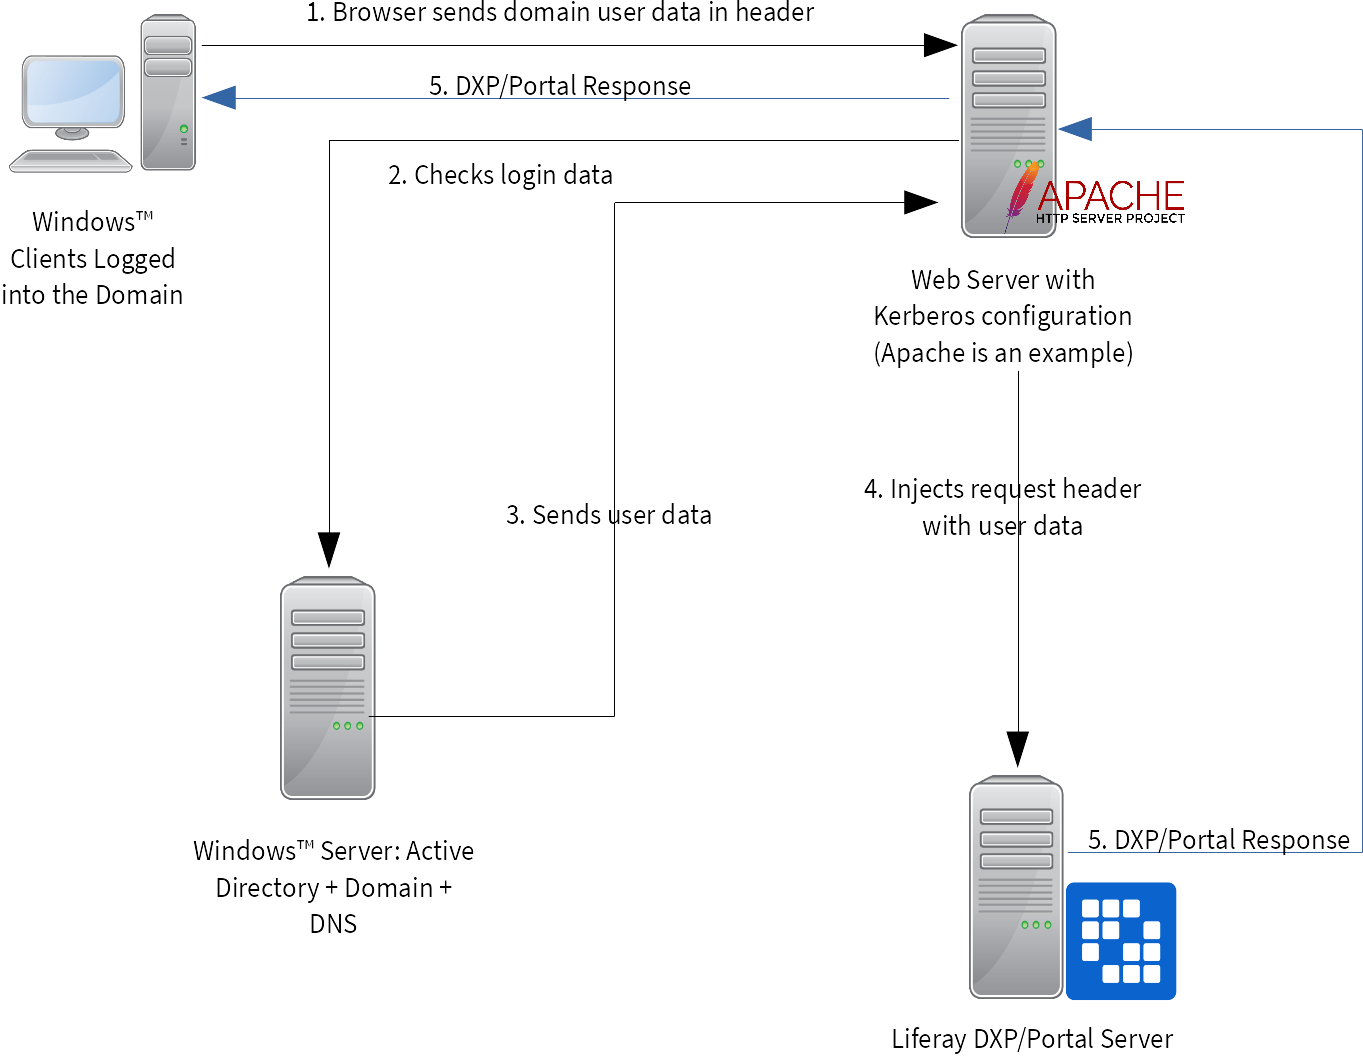
\includegraphics{./images/kerberos.png}
\caption{Kerberos authentication requires a web server in front of your
Liferay DXP server.}
\end{figure}

First, a properly configured web browser sends a negotiate request using
encrypted Windows user data. To configure this, the browser must
recognize the site as a trusted site (explained below). The web server's
Kerberos module uses the keytab file to bind over the Kerberos protocol
to AD and verify the user information. If all is okay, the AD server
confirms the connection with a valid response.

The web server you choose must support both the Kerberos protocol and
the injection of a custom header into the request that Liferay DXP can
later read. When the web server forwards the request to Liferay DXP, it
reads the header to obtain the user data and authenticate the user.

Next, you'll learn how to get all of this working.

\subsection{Configuring Kerberos
Authentication}\label{configuring-kerberos-authentication}

There are four components to configure: a user keytab from Active
Directory, a web server in front of your application server, Liferay
DXP, and your Windows™ clients.

\subsection{Creating the User Keytab}\label{creating-the-user-keytab}

\begin{enumerate}
\def\labelenumi{\arabic{enumi}.}
\item
  Create a user so Liferay DXP can bind to Active Directory.
\item
  Generate a Kerberos keytab file using \texttt{ktpass}:

\begin{verbatim}
ktpass -princ HTTP/[web server host name]@[domain] -mapuser [user name]@[domain] -crypto ALL -ptype KRB5_NT_PRINCIPAL -pass [password] -out c:\kerberos.keytab
\end{verbatim}

  For example:

\begin{verbatim}
ktpass -princ HTTP/mywebserver.intdomain.local@INTDOMAIN.LOCAL -mapuser Marta@INTDOMAIN.LOCAL -crypto ALL -ptype KRB5_NT_PRINCIPAL -pass password-for-Marta -out c:\kerberos.keytab
\end{verbatim}
\item
  Ensure that the AD domain controller and the web server can see each
  other on the network via DNS configuration or \texttt{hosts} file.
\end{enumerate}

\subsection{Configuring Your Web
Server}\label{configuring-your-web-server}

\begin{enumerate}
\def\labelenumi{\arabic{enumi}.}
\item
  Configure Kerberos authentication. On Linux, this involves installing
  \texttt{krb5} and configuring it to match your realm that's already
  configured for Active Directory. The example domain for the user
  configured in step two above would look like this:

\begin{verbatim}
[libdefaults]
    default_realm = INTDOMAIN.LOCAL

[domain_realm]
    mywebserver.intdomain.local = INTDOMAIN.LOCAL
    intdomain.local = INTDOMAIN.LOCAL
    .intdomain.local = INTDOMAIN.LOCAL

[realms]
INTDOMAIN.LOCAL = {
    admin_server = winserver.intdomain.local
    kdc = winserver.intdomain.local
}
\end{verbatim}
\item
  Copy the keytab file you generated on your AD server to your web
  server.
\item
  Configure your web server, making sure you set the correct server
  name, Kerberos service name, Kerberos authentication realms, and the
  path to the keytab file. For example, if you're using the Apache HTTP
  server, the configuration might look like this:

\begin{verbatim}
LoadModule headers_module /usr/lib/apache2/modules/mod_headers.so
LoadModule rewrite_module /usr/lib/apache2/modules/mod_rewrite.so
LoadModule proxy_module /usr/lib/apache2/modules/mod_proxy.so
LoadModule proxy_http_module /usr/lib/apache2/modules/mod_proxy_http.so
LoadModule proxy_ajp_module /usr/lib/apache2/modules/mod_proxy_ajp.so
LoadModule auth_kerb_module /usr/lib/apache2/modules/mod_auth_kerb.so

<VirtualHost *:10080>
    <Proxy *>
        Order deny,allow
        Allow from all
    </Proxy>
    ProxyRequests     Off
    ProxyPreserveHost On
    ProxyPass / ajp://localhost:8009/
    ProxyPassReverse / ajp://localhost:8009/
    ServerName mywebserver.intdomain.local
    <Location />
                Order allow,deny
                Allow from all
                AuthType Kerberos
                KrbServiceName HTTP/mywebserver.intdomain.local@INTDOMAIN.LOCAL
                AuthName "Domain login"
                KrbAuthRealms INTDOMAIN.LOCAL
                Krb5KeyTab /etc/apache2/kerberos.keytab
                require valid-user
                KrbMethodNegotiate  On
                KrbMethodK5Passwd   Off
                #KrbLocalUserMapping On

                # Below directives put logon name of authenticated user into http header X-User-Global-ID
                RequestHeader unset X-User-Global-ID
                RewriteEngine On
                RewriteCond   %{LA-U:REMOTE_USER} (.+)
                RewriteRule   /.* - [E=RU:%1,L,NS]
                RequestHeader set X-User-Global-ID %{RU}e

                # Remove domain suffix to get the simple logon name
                #RequestHeader edit X-User-Global-ID "@INTLAND.LOCAL$" ""

    </Location>
</VirtualHost>
Listen 10080
\end{verbatim}
\end{enumerate}

\subsection{Connecting Liferay DXP to Active Directory over
LDAP}\label{connecting-liferay-dxp-to-active-directory-over-ldap}

\begin{enumerate}
\def\labelenumi{\arabic{enumi}.}
\item
  Finally, configure Liferay DXP to access Active Directory via the LDAP
  protocol. Change authentication to be by Screen Name by selecting it
  in Configuration → Instance Settings → Authentication → General.
\item
  Connect Liferay DXP to AD over LDAP by going to Configuration →
  Instance Settings → Authentication → LDAP and adding an LDAP server.
  Provide the information appropriate to your installation:

  \textbf{Base Provider URL:} Your AD server on the proper port.

  \textbf{Base DN:} Your domain configuration. The example above might
  be \texttt{DC=INTDOMAIN.DC=LOCAL}.

  \textbf{Principal/Credentials:} Supply the credentials for the user
  exported to the keytab file.

  \textbf{Authentication Search Filter:} Supply the appropriate search
  filter to return user objects. For example,
  \texttt{(\&(objectCategory=person)(sAMAccountName=*))}

  \textbf{UUID:} Supply what uniquely identifies a user, such as
  \texttt{sAMAccountName}.

  \textbf{Screen Name:} Supply the field that should be mapped to
  Liferay DXP's screen name field, such as \texttt{sAMAccountName}.

  \textbf{Password:} Supply the field that contains the user's password,
  such as \texttt{userPassword}.
\item
  Be sure to test the connection, save, and enable the configuration.
\item
  Finally, configure the token for single sign-on at Configuration →
  System Settings → Foundation → Token Based SSO. Make sure the User
  Token Name matches \emph{exactly} the token you configured in your web
  server. Click the \emph{Enabled} and \emph{Import from LDAP} boxes and
  click \emph{Save}.
\end{enumerate}

Excellent! You've configured your servers. All that's left is to
configure your clients.

\subsection{Configuring your Clients}\label{configuring-your-clients}

You must do two things: make your computer log into the domain and
configure your Liferay DXP server as a trusted Internet site.

\begin{enumerate}
\def\labelenumi{\arabic{enumi}.}
\item
  Join your computer to your domain. In keeping with the example above,
  you'd make your computer a member of the \texttt{INTDOMAIN.LOCAL}
  domain.
\item
  Log in as a user in that domain.
\item
  Internet Explorer, Edge, and Chrome use the Windows™ settings for
  trusted sites. If you use these browsers, go to Internet Options →
  Security → Local Intranet Sites and add your Liferay DXP server's URL.
  For example, add \texttt{http://mywebserver.intdomain.local:10080}.
\item
  Firefox can be configured by typing \texttt{about:config} in its
  address bar. Search for the below two preferences and add the Liferay
  DXP server's URL as the value for both:

  \begin{itemize}
  \tightlist
  \item
    \texttt{network.negotiate-auth.delegation-uris}
  \item
    \texttt{network.negotiate-auth.trusted-uris}
  \end{itemize}
\end{enumerate}

After configuring these things, test your configuration by accessing
Liferay DXP through the web server's URL. Since you are already logged
into your client machine, you should be automatically logged into
Liferay DXP without a user/password prompt.

Congratulations on configuring Kerberos with Liferay DXP!

\chapter{Enabling Antivirus Scanning for Uploaded
Files}\label{enabling-antivirus-scanning-for-uploaded-files}

You can automatically scan any file uploaded to Liferay for viruses.
When you enable the antivirus scanner, it checks files on upload to
Liferay applications, such as Documents and Media, Message Boards, and
more. Virus-infected files are reported for users to reject.

\begin{figure}
\centering
\includegraphics{./images-dxp/clamd-virus-detected.png}
\caption{The scanner detects virus-infected files on upload to Documents
and Media and other Liferay applications.}
\end{figure}

Liferay DXP 7.0 Fix Pack 96+ (and Service Pack 55+) integrates with the
\href{https://www.clamav.net/documents/scanning\#clamd}{ClamAV Daemon}
(Clamd) running on a separate server.

\textbf{Note:} Prior to Liferay DXP 7.0 Fix Pack 96, the ClamAV
antivirus scanner ran locally. Now Liferay DXP delegates antivirus
scanning to a separate server.

Here's how to enable the Clamd antivirus scanner:

\begin{enumerate}
\def\labelenumi{\arabic{enumi}.}
\item
  On a separate server,
  \href{https://www.clamav.net/documents/scanning\#clamd}{configure and
  start Clamd}.

  \textbf{Important:} Load your ClamAV database before starting Clamd.
\item
  Enable antivirus for your File Store (Document Library) by setting the
  following portal property or
  \href{https://learn.liferay.com/dxp/7.x/en/installation-and-upgrades/installing-liferay/using-liferay-docker-images/configuring-containers.html\#using-liferay-env-variables}{Docker
  Environment variable}.

  Portal property:

\begin{verbatim}
dl.store.antivirus.enabled=true
\end{verbatim}

  Environment variable:

\begin{verbatim}
-e LIFERAY_DL_PERIOD_STORE_PERIOD_ANTIVIRUS_PERIOD_ENABLED=true
\end{verbatim}
\item
  Start your Liferay DXP server.
\item
  Go to \emph{Control Panel} → \emph{System Settings}, and select
  \emph{Antivirus} in the \emph{Security} category.

  \begin{figure}
  \centering
  \includegraphics{./images-dxp/clamd-antivirus-system-settings.png}
  \caption{Antivirus is in the Security category in System Settings.}
  \end{figure}
\item
  Select \emph{Antivirus Clamd Scanner} in the menu.

  \begin{figure}
  \centering
  \includegraphics{./images-dxp/clamd-setup.png}
  \caption{Antivirus Clamd Scanner configuration}
  \end{figure}
\item
  Enter the Clamd server's hostname or IP address, port, and a
  connection timeout time (milliseconds).
\item
  Click \emph{Save}.
\end{enumerate}

Now files are scanned on upload to Liferay applications. If a virus is
detected in a file you're uploading, the scanner reports the infected
file, you should decline saving the file.

\begin{figure}
\centering
\includegraphics{./images-dxp/clamd-virus-detected-message.png}
\caption{Here's the virus detection message.}
\end{figure}

\textbf{Important:} Never save a virus-infected file. Reject the file by
canceling the current operation.

\chapter{Maintaining Liferay DXP}\label{maintaining-liferay-dxp}

Once you have a Liferay DXP installation, there are some things you must
do to keep it running smoothly. Backing up your installation in case of
a hardware failure protects your data and helps you get your system back
in working order quickly. And if you're a DXP customer, patching your
system regularly brings the latest bug fixes to your running instance.

\noindent\hrulefill

Upgrading 7.0 to a new GA version can require
\href{/docs/7-0/deploy/-/knowledge_base/d/upgrading-to-liferay-7}{data
upgrade}. Until you perform all required data upgrades (if any), Liferay
DXP startup fails with messages like these:

\begin{verbatim}
 2018-11-05 17:22:35.025 INFO  [main][StartupHelper:72] There are no patches installed
 You must first upgrade to 7.0
 2018-11-05 17:22:35.098 ERROR [main][MainServlet:277] java.lang.RuntimeException: You must first upgrade to 7.0
\end{verbatim}

\noindent\hrulefill

Read on to learn about how to keep your system running well.

\chapter{Patching Liferay DXP}\label{patching-liferay-dxp}

While we strive for perfection with every Liferay DXP release, the
reality of the human condition dictates that releases may not be as
perfect as originally intended. But we've planned for that. Included
with every Liferay DXP bundle is a Patching Tool that handles installing
two types of patches: fix packs and hotfixes.

\noindent\hrulefill

\textbf{Important:} Make sure to
\href{/docs/7-0/deploy/-/knowledge_base/d/backing-up-a-liferay-installation}{back
up your Liferay DXP installation and database} regularly, especially
before patching. The patching tool installs code changes and some of
these make data changes (if necessary) automatically on startup.

Certain fix packs (service packs) can include data/schema micro
changes---they're optional and revertible. Module upgrades are applied
at server startup by default, or can be applied manually by
\href{/docs/7-0/deploy/-/knowledge_base/d/running-the-upgrade-process\#configuring-non-core-module-upgrades}{disabling
the \texttt{autoUpgrade} property}. You can apply any upgrades using the
\href{/docs/7-0/deploy/-/knowledge_base/d/upgrading-to-liferay-7}{upgrade
tool} before server startup.

\noindent\hrulefill

\noindent\hrulefill

\textbf{Note:}
\href{/docs/7-0/deploy/-/knowledge_base/d/updating-a-cluster}{Patching a
cluster} requires additional considerations.

\chapter{Patching Basics}\label{patching-basics}

Liferay ships 7.0 fixes through three different channels:

\begin{itemize}
\tightlist
\item
  Fix packs
\item
  Hotfixes
\item
  Service Packs
\end{itemize}

\section{Fix Packs}\label{fix-packs}

On a regular schedule, the latest fixes that patch the core are bundled
together into fix packs that are provided to all of Liferay's customers.
Fix packs include fixes for both the core and the application suites
that ship with the product. Each fix pack contains all previous fix
packs since the last service pack.

\href{https://help.liferay.com/hc/en-us/articles/360035038331}{Security
Fix Packs} are a special fix pack type for deploying critical security
fixes quickly without changing fix pack levels.

\section{Hotfixes}\label{hotfixes}

A hotfix is provided to customers when they contact Liferay about an
emergency situation, and Liferay's support team--working with the
customer-- determines that the problem is an issue with the product that
needs to be fixed very quickly. Support fixes the bug and provides a
hotfix to the customer immediately. This is a short-term fix Hotfixes
can patch both the core and the application suites.

\section{Service Packs}\label{service-packs}

Service packs are built on the top of the original Liferay DXP release
and repackaged with the latest fix pack, Patching Tool and modules.
Since a service pack contains the latest fix pack, it contains all
previous fix packs since the last service pack. If starting a new
project, always start with the latest service pack.

Rather than use the service packs to keep existing systems updated,
existing customers should

\begin{enumerate}
\def\labelenumi{\arabic{enumi}.}
\item
  Keep their systems up-to-date with fix packs (according to their own
  deployment schedules).
\item
  Install the latest Marketplace updates frequently.
\item
  Update the Patching Tool when necessary.
\end{enumerate}

This method updates the installation to the service pack levels, while
allowing scheduled deployments and preventing full environment rebuilds.

\section{How Patches are Tested}\label{how-patches-are-tested}

Liferay extensively tests all three types of fix packs to ensure high
quality. For each issue fixed, fix packs go through both automated
regression testing and manual testing. Hotfixes receive similar
automated testing, and the fix for the reported issue is tested by the
support engineer who fixed it.

Before releasing a service pack, test suites run on the packaged
releases to ensure the quality of the packaging.

\chapter{Configuring the Patching
Tool}\label{configuring-the-patching-tool}

Liferay DXP patches can be installed by using the Patching Tool. In the
prepackaged Liferay DXP installation (bundles), the Patching Tool is
already configured. If you've installed Liferay DXP manually, however,
you must also configure the Patching Tool manually. Read on to learn how
to do that. If you're using a bundle, you can skip this section.

\section{Patching Tool Basic
configuration}\label{patching-tool-basic-configuration}

There are two ways to configure the Patching Tool:

\begin{enumerate}
\def\labelenumi{\arabic{enumi}.}
\item
  Automatically by executing the \texttt{auto-discovery} command
\item
  Manually by editing the configuration file (see the Advanced
  Configuration section)
\end{enumerate}

Automatic configuration generates the configuration files by looking for
Liferay DXP files in the file system. By default the Patching Tool looks
for the Liferay DXP files in the parent folder. To start the process run

\begin{verbatim}
patching-tool auto-discovery
\end{verbatim}

If Liferay DXP is not installed in the parent folder, you can specify
its location:

\begin{verbatim}
patching-tool auto-discovery /opt/Liferay/tomcat-8.0.32
\end{verbatim}

That's it! Now that you've installed the Patching Tool and run
auto-discovery, you're ready to download and install patches. You can
install patches manually or automatically.

If you specified the wrong folder or Liferay DXP is not installed in the
parent folder, the Patching Tool won't be able to find the
\href{/docs/7-0/deploy/-/knowledge_base/d/installing-product\#liferay-home}{Liferay
Home} folder and shows an error:

\begin{verbatim}
The .liferay-home has not been detected in the given directory tree.

Configuration:
patching.mode=binary
war.path=../tomcat-8.0.32/webapps/ROOT/
global.lib.path=../tomcat-8.0.32/lib/ext/
liferay.home=**[please enter manually]**

The configuration hasn't been saved. Please save this to the default.properties file.
\end{verbatim}

In this case you can either add the folder manually to the configuration
or create the \texttt{.liferay-home} file and re-run the auto-discovery
process.

When the patching tool is configured, you can run
\texttt{patching-tool\ info} and receive information about the product
version.

\section{Patching Tool Advanced
Configuration}\label{patching-tool-advanced-configuration}

By default, the Patching Tool's configuration file is in its
installation folder and called \texttt{default.properties}.

A Patching Tool configuration file typically looks like this:

\begin{verbatim}
patching.mode=binary
war.path=../tomcat-8.0.32/webapps/ROOT/
global.lib.path=../tomcat-8.0.32/lib/ext/
liferay.home=../
\end{verbatim}

The properties above (described fully
\hyperref[using-profiles-with-the-patching-tool]{below}) define the
location of
\href{/docs/7-0/deploy/-/knowledge_base/d/installing-product\#liferay-home}{Liferay
Home}, the patching mode (binary or source), the path to where WAR files
are deployed in the app server, and the global library path. If
auto-discovery found your Liferay Home folder, the location of Liferay
DXP's OSGi-based module framework can be calculated from this. If,
however, you customized the folder structure, you'll have to specify
manually the following properties:

\begin{verbatim}
module.framework.core.path=path_to_modules_core_dir
module.framework.marketplace.path=path_to_modules_marketplace_dir
module.framework.modules.path=path_to_modules_modules_dir
module.framework.portal.path=path_to_modules_portal_dir
module.framework.static.path=path_to_modules_static_dir
\end{verbatim}

For most installations, you don't have to do this, as the \texttt{osgi}
folder is in its default location. If you've customized the location of
the module framework, however, you'll have to specify the above
locations. Since you moved them, you should know where they are.

\subsection{Using Profiles with the Patching
Tool}\label{using-profiles-with-the-patching-tool}

When you ran the auto-discovery task after installing the Patching Tool,
it created a default profile that points to the application server it
discovered. This is the easiest way to use the Patching Tool, and is
great for smaller, single server installations. But many Liferay DXP
installations are sized to serve millions of pages per day, and the
Patching Tool has been designed for this as well. So if you're running a
small, medium, or large cluster of Liferay DXP machines, you can use the
Patching Tool to manage all of them using profiles.

The auto-discovery task creates a properties file called
\texttt{default.properties}. This file contains the detected
configuration for your application server. But you're not limited to
only one server which the tool can detect. You can have it auto-discover
other runtimes, or you can manually create new profiles yourself.

To have the Patching Tool auto-discover other runtimes, you must use a
few more command line parameters:

\begin{verbatim}
./patching-tool.[sh|bat] [name of profile] auto-discovery [path/to/runtime]
\end{verbatim}

This runs the same discovery process, but on a path you choose, and the
profile information goes into a
\texttt{{[}name\ of\ profile{]}.properties} file.

Alternatively, you can manually create your profiles. Using a text
editor, create a \texttt{{[}profile\ name{]}.properties} file in the
same folder as the Patching Tool script.

Below is a description of all the supported properties.

\subsection{Configuration Properties}\label{configuration-properties}

\textbf{patching.mode:} This can be \texttt{binary} (the default) or
\texttt{source}, if you're patching a source tree. Liferay DXP patches
contain both binary and source patches. If your development team is
extending Liferay DXP, you'll want to provide the patches you install to
your development team so they can patch their source tree.

\textbf{patches.folder:} Specify the location where you'll copy your
patches. By default, this is \texttt{./patches}.

\textbf{war.path:} Specify the location of the Liferay DXP installation
inside your application server. Alternatively, you can specify a .war
file here, and you can patch a Liferay DXP .war for installation to your
application server.

\textbf{global.lib.path:} Specify the location where \texttt{.jar} files
on the global classpath are stored. If you're not sure, search for your
\texttt{portal-kernel.jar} file; it's on the global classpath. This
property is only valid if your \texttt{patching.mode} is
\texttt{binary}.

\textbf{liferay.home:} Specify the location where by default the
\texttt{data}, \texttt{osgi}, and \texttt{tools} folders reside.

\textbf{source.path:} Specify the location of your Liferay DXP source
tree. This property is only valid if your \texttt{patching.mode} is
\texttt{source}.

\noindent\hrulefill

\textbf{Note:} To patch the 7.0 source code, please upgrade to Patching
Tool 2.0.4+.

\noindent\hrulefill

Service Pack detection is available behind a proxy server. Use the
following settings to configure your proxy:

\begin{verbatim}
### Proxy settings

# HTTP Proxy

#proxy.http.host=192.168.211.39
#proxy.http.port=80
#proxy.http.user=user
#proxy.http.password=password

# HTTPS Proxy

proxy.https.host=192.168.211.39
proxy.https.port=808
proxy.https.user=user
proxy.https.password=password

# SOCKS Proxy

#proxy.socks.host=192.168.211.39
#proxy.socks.port=1080
#proxy.socks.user=user
#proxy.socks.password=password
\end{verbatim}

You can have as many profiles as you want and use the same Patching Tool
to patch all of them. This helps to keep all your installations in sync.

\section{Installing patches on the 7.0
WAR}\label{installing-patches-on-the-7.0-war}

Because of your app server choice, you may not be able to patch the
Liferay DXP instance that's installed, because the files aren't
available on the file system. Instead, you must patch the Liferay DXP
WAR file and then re-deploy it. This tutorial shows you how to do that.

\subsection{Prerequisites}\label{prerequisites}

Download the necessary artifacts from the
\href{https://web.liferay.com/group/customer/dxp/downloads/digital-enterprise}{Customer
Portal:}

\begin{itemize}
\tightlist
\item
  Liferay DXP WAR (liferay-dxp-digital-enterprise-{[}version{]}.war)
\item
  OSGi dependencies
  (liferay-dxp-digital-enterprise-dependencies-{[}version{]}.zip)
\item
  Additional dependencies
  (liferay-dxp-digital-enterprise-osgi-{[}version{]}.zip)
\item
  Latest Patching Tool
\end{itemize}

\subsection{How to Install a Fix Pack on the Liferay DXP
WAR}\label{how-to-install-a-fix-pack-on-the-liferay-dxp-war}

\begin{enumerate}
\def\labelenumi{\arabic{enumi}.}
\item
  Create a folder and unzip the dependency artifacts and the Patching
  Tool into it. Content of this folder should look like this:

  \begin{figure}
  \centering
  \includegraphics{./images-dxp/patch-war-file-folder-structure.png}
  \caption{Use a simple folder structure for patching.}
  \end{figure}
\item
  Create the default profile configuration file in the Patching Tool's
  home folder:
  \texttt{liferay-de-home/patching-tool/default.properties}. The
  contents should look like this:

\begin{verbatim}
patching.mode=binary
war.path=/liferay-de-home/liferay-dxp-digital-enterprise-[version].war
global.lib.path=/liferay-de-home/liferay-dxp-digital-enterprise-dependencies-[version]/
liferay.home=/liferay-de-home/
\end{verbatim}

  If you have different OSGi folder structure, you can specify them as
  described in the documentation
  \href{/docs/7-0/deploy/-/knowledge_base/d/patching-tool-advanced-configuration}{Patching
  Tool Advanced Configuration}:

\begin{verbatim}
module.framework.core.path=d:/liferay-de-home/osgi/core
module.framework.marketplace.path=d:/liferay-de-home/osgi/marketplace
module.framework.modules.path=d:/liferay-de-home/osgi/modules
module.framework.portal.path=d:/liferay-de-home/osgi/portal
module.framework.static.path=d:/liferay-de-home/osgi/static 
\end{verbatim}
\item
  Download the patch (fix pack or hotfix) that you'd like to install and
  place it to the Patching Tool's \texttt{patches} folder without
  unzipping it.
\item
  Now the Patching Tool info command shows the following output:

\begin{verbatim}
/liferay-de-home/patching-tool>patching-tool.bat info

Loading product and patch information...
Product information:
  * installation type: binary
  * build number: 7010
  * service pack version:
    - available SP version: Not available
    - installable SP version: 1
  * patching-tool version: 2.0.5
  * time: 2016-12-05 13:29Z
  * plugins: no plugins detected

Currently installed patches: -

Available patches: de-8-7010

Detailed patch list:
  [ I] de-8-7010 :: Currently not installed; Will be installed.
\end{verbatim}
\item
  Install the downloaded patch.

\begin{verbatim}
/liferay-de-home/patching-tool>patching-tool.sh install
One patch is ready to be installed. Applying de-8...
Cleaning up: [1%..10%..20%..30%..40%..50%..60%..70%..80%..90%..100%]
Installing patches: [1%..10%..20%..30%..40%..50%..60%..70%..80%..90%...100%]
The installation was successful. One patch is installed on the system.
\end{verbatim}
\end{enumerate}

Great! You have successfully patched the artifacts, and they are ready
to be deployed on any supported Application Server.

\subsection{Related Topics}\label{related-topics-9}

\href{/docs/7-0/deploy/-/knowledge_base/d/patching-tool-advanced-configuration}{Patching
Tool Advanced Configuration}

\href{https://help.liferay.com/hc/en-us/articles/360017895792-Introduction-to-Deploying-Liferay-DXP}{Deploying
Liferay DXP}

\href{/docs/7-0/deploy/-/knowledge_base/d/installing-liferay-dxp-on-weblogic-12c-r2}{Installing
Liferay DXP on WebLogic 12c R2}

\href{/docs/7-0/deploy/-/knowledge_base/d/installing-liferay-dxp-on-websphere-8-5-5}{Installing
Liferay DXP on WebSphere 8.5.5}

\chapter{Using the Patching Tool}\label{using-the-patching-tool}

If you're using a Liferay DXP bundle, the Patching Tool is already
installed. When an update is necessary to install a patch, the Patching
Tool automatically asks for an update.

You follow the same procedure whether you're installing or upgrading the
Patching Tool. Once you've obtained it from the Customer Portal, unzip
it anywhere in the file system. Generally it's a good idea to keep it
together with the Liferay DXP installation.

Upgrading is easy: override the previous Patching Tool with newest one
by unzipping it on top of the old version.

\section{Executables}\label{executables}

The Patching Tool is a Java based application. The distribution contains
shell/ .bat scripts to make it easier to use. On Unix systems you can
run

\begin{verbatim}
./patching-tool.sh parameters
\end{verbatim}

On Windows, run

\begin{verbatim}
patching-tool parameters
\end{verbatim}

The latter method appears in the examples below. On Unix, replace the
name of the executable before running the scripts.

\section{Installing Patches}\label{installing-patches}

The first thing you must do when installing patches is to shut down your
server. On Windows operating systems, files that are in use are locked
by the OS, and can't be patched. On Unix-style systems, you can usually
replace files that are running, but that still leaves the old ones
loaded in memory. So your best bet is to shut down the application
server that's running Liferay DXP before you install a patch.

Liferay distributes patches as \texttt{.zip} files, whether they are
hotfixes or fix packs. When you receive one, either via a
\href{https://help.liferay.com/hc}{Help Center} ticket (hotfix) or
through downloading a fix pack from the
\href{https://web.liferay.com/group/customer}{Customer Portal}, place it
in the Patching Tool's \texttt{patches} folder (e.g.,
\texttt{{[}Liferay\ Home{]}/patching-tool/patches}) without unzipping
it. Once you've done that, it's a simple matter to install it. First,
execute

\begin{verbatim}
patching-tool info
\end{verbatim}

This displays a list of patches you've already installed, along with a
list of patches that \emph{can} be installed from what's in the
\texttt{patches} folder.

To install the available patches, use the following steps. First, issue
the following command:

\begin{verbatim}
patching-tool install
\end{verbatim}

To make sure the all changed OSGi bundles replace the existing ones, it
is recommended to delete the \texttt{osgi/state} folder from the
\href{/docs/7-0/deploy/-/knowledge_base/d/installing-product\#liferay-home}{Liferay
Home folder}.

\noindent\hrulefill

\textbf{Important}: The \texttt{osgi/state} folder should ONLY be
deleted when working in a development environment or when applying a fix
pack or hot fix.

\noindent\hrulefill

\noindent\hrulefill

\textbf{Note}: The \texttt{osgi/state} folder in the contains OSGi
bundle state information. If an OSGi bundle's changes in a hot fix or
fix pack are internal only and are, therefore, invisible to the OSGi
framework, that OSGi bundle stays installed and its state information
stays unchanged. Hot fixes, for example, may contain in-place changes
that do not use the API---the framework cannot detect such changes. A
fix pack's changes may also be transparent to the framework. For these
reasons, deleting the \texttt{osgi/state} folder after applying fix
packs and hot fixes is recommended.

\noindent\hrulefill

If there are new database indexes created by the patch, the Patching
Tool tells you to update them. To get the list, run this command:

\begin{verbatim}
patching-tool index-info
\end{verbatim}

Since there's no database connection at patching time, the indexes must
be created at portal startup. To have the indexes created automatically,
add the following line to the \texttt{portal-ext.properties} file if the
server has permissions to modify the indexes on the database:

\begin{verbatim}
database.indexes.update.on.startup=true
\end{verbatim}

Otherwise, you must create the indexes manually. Check the output of the
\texttt{patching-tool\ index-info} command for more details.

Once your patches have been installed, you can verify them by using the
\texttt{patching-tool\ info} command, which now shows your patches in
the list of installed patches.

\noindent\hrulefill

\textbf{Note:} If there are any issues with the installed fixes, verify
that there aren't any remaining files from the previous patch
installation of a fix pack or hotfix within the application server
cache.

\noindent\hrulefill

During the installation, \texttt{patching-backup-deps.zip} and
\texttt{patching-backup.zip} files are created and stored in the
\texttt{ROOT/WEB-INF} folder. These files are necessary to restore the
Liferay DXP's original state; removing them would disable further
patching.

\noindent\hrulefill

\textbf{Note:} When installing patches, Liferay DXP's \texttt{web.xml}
is always overwritten by the one contained in the patch. If you've
customized \texttt{web.xml}, you must re-implement your customizations
after installing a patch.

\noindent\hrulefill

The \texttt{patching-backup.zip} file is necessary for installing future
patches, because the Patching Tool reverts the installed fix pack before
installing a new one. To revert the installed fix pack, it examines the
contents of the \texttt{patching-backup.zip} to determine the changes
that it needs to revert.

\subsection{Handling Hotfixes and
Patches}\label{handling-hotfixes-and-patches}

As stated above, hotfixes are short term fixes provided as quickly as
possible, and fix packs are larger bundles of hotfixes provided to all
customers at regular intervals. If you already have a hotfix installed
and the fix pack that contains that hotfix is released, the Patching
Tool can manage this for you. Fix packs always supersede hotfixes, so
when you install your fix pack, the hotfix that it contains is
uninstalled, and the fix pack version is installed in its place.

Sometimes there can be a fix to a fix pack. This is also handled
automatically. If a new version of a fix pack is released, you can use
the Patching Tool to install it. The Patching Tool uninstalls the old
fix pack and installs the new version in its place.

\subsection{\texorpdfstring{Including `\emph{support-info}' in Help
Center
Tickets}{Including `support-info' in Help Center Tickets}}\label{including-support-info-in-help-center-tickets}

To enable Liferay to reproduce subscriber issues, it is critical that
the patch level in a given environment be made available to Liferay.

To generate the patch level for your environment, use the following
command:

\begin{verbatim}
patching-tool support-info
\end{verbatim}

A text file called
\texttt{patching-tool-support-info-actual-timestamp.txt} is created in
the patching-tool folder. Please upload this file to the
\href{https://help.liferay.com/hc}{Help Center} ticket.

\subsection{Fix Pack Dependencies}\label{fix-pack-dependencies}

Some hotfixes require a fix pack to be installed first. If you attempt
to install a hotfix that depends on a fix pack, the Patching Tool
notifies you. Go to the customer portal and obtain the hotfix
dependency. Once all the necessary patches are available in the
\texttt{patches} folder, the Patching Tool installs them.

The Patching Tool can also remove patches.

\section{Removing or Reverting
Patches}\label{removing-or-reverting-patches}

Have you noticed that the Patching Tool only seems to have an
\texttt{install} command? This is because patches are managed not by the
command, but by what appears in the \texttt{patches} folder. You manage
the patches you have installed by adding or removing patches from this
folder. If you currently have a patch installed that you don't want,
remove it from the \texttt{patches} folder. When you run the
\texttt{patching-tool\ install} command, and the patch is removed.

If you want to remove all patches you've installed, use the
\texttt{./patching-tool.sh\ revert} command. This removes all patches
from your installation.

Prior to Fix Pack 13, the OSGi state folder could retain obsolete
bundles in its cache. If you're running a version prior to Fix Pack 13,
delete the \emph{osgi/state} folder in Liferay Home.

\section{Cleaning Up}\label{cleaning-up}

After you've performed your patching procedure (whether you've installed
or removed patches), it's important to clean up Liferay DXP's cache of
deployed code. This ensures that when you start the server, you're using
the revision you've just installed the patches for. This is really easy
to do.

In the Liferay Home folder is a folder called \texttt{work}. Remove the
contents of this folder to clear out the cached code. Now you're ready
to start your server.

\section{Comparing Patch Levels}\label{comparing-patch-levels}

If you're a developer, the Patching Tool can show you what changed
between different versions. These commands show you information about
the different patch levels:

\texttt{patching-tool\ diff}: Prints the differences between two patch
levels. At least one stored patch level must be available. This command
accepts options for filtering the output:

\begin{itemize}
\tightlist
\item
  \texttt{source}: Shows the source differences between the two patch
  levels.
\item
  \texttt{files}: Shows a list of the modified files.
\item
  \texttt{fixed-issues}: Shows a list of LPS/LPE issues from our issue
  tracking system.
\end{itemize}

For detailed usage information, run \texttt{patching-tool\ help\ diff}.

\texttt{patching-tool\ store}: Manages patching level information for
the \texttt{diff} command. Your patches must contain source code to
store the patch level and to prepare usable information for the
\texttt{diff} command. Here are the \texttt{store} command options:

\begin{itemize}
\tightlist
\item
  \texttt{info}: Prints the list of patches which make up the stored
  patch level.
\item
  \texttt{add}: Stores the patch level that can be found in the patches
  directory.
\item
  \texttt{update}: Adds or updates patch level information.
\item
  \texttt{rm}: Removes previously stored patch level information.
\end{itemize}

For detailed usage information, run \texttt{patching-tool\ help\ store}.

\section{Showing collisions between patches and deployed
plugins}\label{showing-collisions-between-patches-and-deployed-plugins}

Some patches update files you might have customized via a plugin. The
\texttt{patching-tool\ list-collisions} command lists differences
(collisions) between installed patch files and your plugin's version of
them. Here's the command:

\begin{verbatim}
patching-tool list-collisions
\end{verbatim}

It is an alias for the following diff command:

\begin{verbatim}
patching-tool diff collisions files _base
\end{verbatim}

\texttt{\_base} is the literal patch level name. Collisions are only
listed for installed patches that contain source code files.

\noindent\hrulefill

\textbf{Note:} As of Patching Tool 2.0.9,
\texttt{patching-tool\ list-collisions} lists only JSP file collisions
in fragment bundles.

\noindent\hrulefill

\section{Separating the Patches from the Liferay DXP
Installation}\label{separating-the-patches-from-the-liferay-dxp-installation}

As of Patching Tool 2.0.6, there's a feature that helps reduce the
patched Liferay DXP bundle size. If the bundle has been patched, you can
make it smaller by moving the restore files out of it.

Patched bundles are large because the restore files by default are
stored inside the web application's WEB-INF folder. These files are
required for patching the Liferay DXP instance again.

If these files were removed, subsequent patching processes would fail.
Because of this, Liferay added an option to separate the patching files
from the Liferay DXP bundle while still preserving restoring them safely
when new patches arrive. To do this, you use this command:

\begin{verbatim}
patching-tool separate [separation_name] 
\end{verbatim}

This command produces a
\texttt{liferay-patching-files-{[}separation-name{]}.zip}file in the
Patching Tool's \texttt{patches} folder. It contains the necessary files
and metadata for patching, verification, and validation. Once you create
this file, the patch files are removed from their default location and
are now only available in this file. You can now move the file elsewhere
to make the bundle's size smaller.

\textbf{WARNING:} If the product is separated from its patches in this
way, you cannot run most of the Patching Tool commands until the patches
are restored.

After the separation process only the following commands can be used:

\begin{itemize}
\tightlist
\item
  auto-discovery
\item
  info
\item
  setup
\end{itemize}

Any other command returns this:

\begin{verbatim}
This installation does not include data for patching. Please copy the
liferay-patching-files-[separation-name].zip file into the 'patches' directory
and run patching-tool setup. 
\end{verbatim}

This is how you restore the patch files to your system. Details below.

\subsection{Restoring the Separated Patch
Files}\label{restoring-the-separated-patch-files}

When you need to patch Liferay DXP again, you must restore the separated
patch artifact. To do this, copy the
\texttt{liferay-patching-files-{[}separation-name{]}.zip} back to the
Patching Tool's \texttt{patches} folder and run
\texttt{patching-tool\ setup} command.

If the command finds the necessary patching artifact, it restores the
patch files to the bundle. After that, the Patching Tool works like it
did prior to separating the patches.

\chapter{Keeping up with Fix packs and Service
Packs}\label{keeping-up-with-fix-packs-and-service-packs}

The \emph{Announcements} section on
\href{https://help.liferay.com/hc}{Liferay's Help Center page} lists all
fix pack updates, security alerts, product releases, and system updates.
The approximate frequency of fix pack and service pack releases is
explained
\href{/docs/7-0/deploy/-/knowledge_base/d/patching-basics}{here}. The
\emph{Receive Notifications} sidebar lets you subscribe to the latest
updates on products, patches, and system improvements.

Click \emph{Downloads} on the
\href{https://help.liferay.com/hc/en-us/categories/360000872531}{Liferay
Digital Experience Platform page} to access:

\begin{itemize}
\tightlist
\item
  Latest Release
\item
  Fix Packs
\item
  Service Packs Archive
\item
  Security Advisories
\item
  Patching Tool
\end{itemize}

Click \emph{Support Information} to access the compatibility matrix,
support FAQs, and more.

\section{Securing Liferay DXP's Remote
Services}\label{securing-liferay-dxps-remote-services}

Liferay DXP includes a script console which administrators can use to
invoke Liferay DXP's API. See the
\href{/docs/7-0/user/-/knowledge_base/u/running-scripts-from-the-script-console}{Using
Liferay DXP's Script Console} article for more information. Liferay DXP's
API can also be invoked remotely. How is this possible? Liferay DXP
includes a utility called the \emph{Service Builder} which is used to
generate all of the low level code for performing CRUD operations for
entities that are saved to Liferay DXP's database. This utility is
further explained in the tutorial
\href{/docs/7-0/tutorials/-/knowledge_base/t/service-builder}{Service
Builder}. Service Builder generates web service interfaces that can be
invoked remotely. Since Liferay DXP's APIs are generated by Service
Builder, the method signatures and behavior for storing and retrieving
Liferay DXP objects are consistent.

Because the actual method calls for retrieving data are the same
regardless of how one gets access to those methods (i.e., locally or
through web services), Liferay DXP provides a consistent interface for
accessing portal data that few other products can match. The actual
interfaces for the various services can be found by navigating to
Liferay DXP's JSON web services page:
\url{http://localhost:8080/api/jsonws}. Before these services can be
invoked, administrators need to enable users to access these services
remotely.

Liferay DXP includes four layers of web service security:

\begin{itemize}
\tightlist
\item
  IP permission layer
\item
  Service access policy layer
\item
  Authentication/verification layer (browser-only):
\item
  User permission layer
\end{itemize}

Please see the
\href{/docs/7-0/deploy/-/knowledge_base/d/service-access-policies}{Service
Access Policies} documentation for a description of these security
layers.

In the default \texttt{portal.properties} file, there is a section
called \textbf{Main Servlet}. This section defines the security settings
for all of the remote services provided by Liferay DXP. Copy this
section and paste it into your custom \texttt{portal-ext.properties}
file. Then you can edit the default values to configure the security
settings for the Axis Servlet, the Liferay Tunnel Servlet, the Spring
Remoting Servlet, the JSON Tunnel Servlet, and the WebDAV servlet.

By default, a user connecting from the same machine Liferay DXP is
running on can access remote services so long as that user has the
permission to use those services in Liferay DXP's permissions system. Of
course, you are not really ``remote'' unless you are accessing services
from a different machine. Liferay DXP has multiple layers of security
when it comes to accessing its services remotely. Without explicit
rights granted for each layer, attempting to invoke a Liferay DXP API
function remotely fails and a remote exception is thrown.

The first layer of web service security that a user needs to get through
in order to call a method from the service layer is servlet security.
This is the IP permission layer listed above. The \emph{Main Servlet}
section of the \texttt{portal-ext.properties} file is used to enable or
disable access to Liferay DXP's remote services. In this section of the
properties file, there are properties for each of Liferay DXP's remote
services.

You can set each service individually with the security settings that
you require. For example, you may have a batch job which runs on another
machine in your network. This job looks in a particular shared folder on
your network and uploads documents to your site's Documents and Media
portlet on a regular basis, using Liferay DXP's web services. To enable
this batch job to get through the first layer of security, you would
modify the \texttt{portal-ext.properties} file and put the IP address of
the machine on which the batch job is running in the list for that
particular service. For example, if the batch job uses the Axis web
services to upload the documents, you would enter the IP address of the
machine on which the batch job is running to the
\texttt{axis.servlet.hosts.allowed} property. A typical entry might look
like this:

\begin{verbatim}
axis.servlet.hosts.allowed=192.168.100.100, 127.0.0.1, SERVER_IP
\end{verbatim}

If the machine on which the batch job is running has the IP address
\texttt{192.168.100.100}, this configuration will allow that machine to
connect to Liferay DXP's web services and pass in user credentials to be
used to upload the documents.

The second layer of web service security is the service access policy
layer. When attempting to invoke a Liferay DXP API function remotely,
the function must be whitelisted by one of the service access policies
that apply to the request.

The third layer of security is the authentication/verification layer.
This layer is only applied to a Liferay DXP API function invocation
request if the request is coming from a browser. In this case, the
request must include a valid authentication token.

The fourth and final layer of security is Liferay DXP's permissions
system that protects every Liferay DXP entity. The user account that
accesses the services remotely must have the proper permissions to
operate on the objects it attempts to access. Otherwise, a remote
exception is thrown. Portal administrators need to use Liferay DXP's
permissions system to grant access to these resources to the
administrative user account that attempts to operate on them remotely.
For example, suppose that a Documents and Media folder called
\emph{Documents} has been set up in a site. A role has been created
called \emph{Document Uploaders} which has the rights to add documents
to this folder. Your batch job will be accessing Liferay DXP's web
services in order to upload documents into this folder. In order for
this to work, you have to call the web service using a user account to
which the \emph{Document Uploaders} role has been assigned (or that has
individual rights to add documents to the folder). Otherwise, you will
be prevented from using the web service.

You can invoke a Liferay DXP web service in a variety of ways. For
example, you can invoke a web service by navigating to a specific URL in
your browser, by using the \href{https://curl.haxx.se/}{cURL} tool, or
via JavaScript. Here's an example URL for a Liferay DXP web service
invocation using a browser:

\begin{verbatim}
http://localhost:8080/api/jsonws/user/get-user-by-email-address/company-id/20154/email-address/test%40liferay.com?p_auth=[value]
\end{verbatim}

This Liferay DXP web service invocation returns the user with the email
address \texttt{test@example.com} in the company (portal instance) with
the ID \texttt{20154}. Note that for the web service invocation to
succeed, you must supply a correct value for the \texttt{p\_auth} URL
parameter. You can find such a value by signing in to Liferay DXP,
navigating to \url{http://localhost:8080/api/jsonws} and clicking on any
function that appears in the list. Use the value for the
\texttt{p\_auth} token that appears under the Execute heading. For more
examples of Liferay DXP web service invocations, please see the
\href{/docs/7-0/tutorials/-/knowledge_base/t/json-web-services-invocation-examples}{JSON
Web Services Invocation Examples} documentation.

Some methods of invoking Liferay DXP web services (e.g., using
\href{https://curl.haxx.se/}{cURL}) allow you to supply a username and
password. Note that \emph{Password Policies} (covered in the
\href{/docs/7-0/user/-/knowledge_base/u/user-management}{User
Management} documentation) can be used in combination with this feature.
If you are enforcing password policies on your users (requiring
passwords to take a certain form, requiring users to change their
passwords on a periodic basis, etc.), any administrative user account
which accesses Liferay DXP's web services in a batch job can have its
password expire too.

To prevent this from happening, you can add a new password policy which
does not enforce the password expiration and add your administrative
user ID to it. Then your batch job can run as many times as you need it
to and the administrative user account's password will never expire.

In summary, accessing Liferay DXP remotely requires the successful
passing of four security checks:

\begin{enumerate}
\def\labelenumi{\arabic{enumi}.}
\tightlist
\item
  The IP address must be pre-configured in the server's
  \texttt{portal-ext.properties} file.
\item
  At least one service access policy which applies to the request must
  have the API function being invoked in a whitelist.
\item
  If a browser is making the web service invocation request, a valid
  authentication token (\texttt{p\_auth} URL parameter) must be
  provided.
\item
  The user ID being used must have permission to access the resources it
  attempts to access.
\end{enumerate}

\subsection{Accessing Liferay DXP's JSON Web
Services}\label{accessing-liferay-dxps-json-web-services}

To see which Liferay DXP service methods are registered and available
for use via JSON web services, open your browser to the following
address:

\begin{verbatim}
http://localhost:8080/api/jsonws
\end{verbatim}

The page lists the portal's registered and exposed service methods. Get
each method's details by clicking the method name. You can view the full
signature of each method, all its arguments, the exceptions that can be
thrown, and its Javadoc! Using a simple form from within your browser,
you can even invoke the service method for testing purposes.

To list registered services on a plugin (e.g.~a custom portlet), don't
forget to use its context path in your URL:

\begin{verbatim}
http://localhost:8080/[plugin-context]/api/jsonws
\end{verbatim}

This lists the JSON Web Service API for the plugin.

\subsection{Accessing Liferay DXP's
WSDL}\label{accessing-liferay-dxps-wsdl}

After configuring the security settings properly, your first step in
obtaining access to Liferay DXP's remote SOAP web services is to access
the WSDL. If you are on a browser on the same machine Liferay DXP is
running on, you can do this by accessing the following URL:

\begin{verbatim}
http://localhost:[port number]/tunnel-web/axis
\end{verbatim}

If, for example, you are running on Tomcat on port 8080, you would
specify this URL:

\begin{verbatim}
http://localhost:8080/tunnel-web/axis
\end{verbatim}

If you are accessing a web service that was created as part of a portlet
plugin, the URL is similar, but uses the context of your application
rather than the tunnel-web servlet. You can get a list of your Service
Builder-generated WSDL documents by using the URL pattern below:

\begin{verbatim}
http://localhost:8080/your-portlet/axis
\end{verbatim}

If you are on a different machine from the Liferay DXP server, you will
need to pass in your user credentials on the URL to access the WSDL:

\begin{verbatim}
http://[user ID]:[password]@[server name]:[port number]/tunnel-web/axis
\end{verbatim}

In any case, once you successfully browse to this URL, you will see the
list of web services. You can access the WSDL for each service by
clicking on the \emph{WSDL} link next to the name of the service. There
are many services; one for each of the services available from the
Liferay DXP API.

Once you click on one of the \emph{WSDL} links, the Web Service
Definition Language document will be displayed. This document can be
used to generate client code in any language that supports it. You can
either save the document to your local machine and then generate the
client code that way, or use your tool to trigger Liferay DXP to
generate the document dynamically by using one of the URLs above. For
information about developing applications that leverage Liferay DXP's
remote services, please see the
\href{/docs/7-0/tutorials/-/knowledge_base/t/invoking-json-web-services}{Invoking
JSON Web Services} documentation.

\chapter{Backing up a Liferay DXP
Installation}\label{backing-up-a-liferay-dxp-installation}

Once you have an installation of Liferay DXP running, you should
implement a comprehensive backup plan. In case some kind of catastrophic
hardware failure occurs, you'll be thankful to have backups and
procedures for restoring Liferay DXP from one of them. Liferay DXP isn't
very different from other Java web application that might be running on
your application server. Nevertheless, there are some specific
components you should include in your backup plan.

The recommended backup plan includes backing up these things:

\begin{itemize}
\tightlist
\item
  Source code
\item
  Liferay DXP's file System
\item
  Liferay DXP's database
\end{itemize}

\section{Backing up Source Code}\label{backing-up-source-code}

If you have extended Liferay DXP or have written any plugins, they
should be stored in a source code repository such as Git, Subversion, or
CVS, unless you're Linus Torvalds, and then tarballs are okay too
(that's a joke). You should back up your source code repository on a
regular basis to preserve your ongoing work. This probably goes without
saying in your organization since nobody wants to lose source code
that's taken months to produce. Thus you should include source code in
your Liferay DXP backup plan.

Next, let's examine the Liferay DXP installation items you should back
up.

\section{Backing up Liferay's File
System}\label{backing-up-liferays-file-system}

The
\href{/docs/7-0/deploy/-/knowledge_base/d/installing-product\#liferay-home}{Liferay
Home folder} stores Liferay DXP's properties configuration files, such
as \texttt{portal-setup-\ wizard.properties} and
\texttt{portal-ext.properties}. You should absolutely back them up. In
fact, it's best to back up your entire application server and Liferay
Home folder contents.

Liferay DXP stores configuration files, search indexes, and cache
information in Liferay Home's \texttt{/data} folder. If you're using the
File System store or the Advanced File System store, the documents and
media repository is also stored here by default. It's always important
to back up your \texttt{/data} folder.

\noindent\hrulefill

\textbf{Important:} If you've configured the document library to store
files to a

\noindent\hrulefill location other than a \texttt{{[}Liferay\ Home{]}/data}
subfolder, back up that location.

The files that comprise Liferay DXP's OSGi runtime are stored in Liferay
Home's \texttt{/osgi} folder. It contains all of the app and module JAR
files deployed to Liferay DXP. The \texttt{/osgi} folder also contains
other required JAR files, configuration files, and log files. It's also
important to back up your \texttt{/osgi} folder.

Liferay Home's \texttt{/logs} folder contains Liferay DXP's log files.
If a problem occurs on Liferay DXP, the Liferay DXP log files often
provide valuable information for determining what went wrong. The
\texttt{/data}, \texttt{/osgi}, and \texttt{/logs} folders are all
contained in the Liferay Home folder. Thus, if you're backing up both
your application server folder and your Liferay Home folder, you're in
good shape.

That covers the Liferay DXP file system locations you should back up.
Next, let's discuss how to back up Liferay DXP's database.

\section{Backing up Liferay DXP's
Database}\label{backing-up-liferay-dxps-database}

Liferay DXP's database is the central repository for all of the portal's
information. It's the most important component to back up. You can back
up the database live (if your database allows this) or by exporting
(dumping) the database into a file and then backing up the exported
file. For example, MySQL ships with a \texttt{mysqldump} utility which
lets you export the entire database and data into a large SQL file. This
file can then be backed up. On restoring the database you can import
this file into the database to recreate the database state to that of
the time you exported the database.

If you're storing Liferay DXP's Documents and Media Library files to a
Jackrabbit JSR-170 repository database, you should back it up. If you've
placed your search index into a database (not recommended; see the
\href{/docs/7-0/deploy/-/knowledge_base/d/liferay-clustering}{Liferay
DXP Clustering} article for information on using Cluster Link or Solr),
you should back up that database too.

If you wish to avoid re-indexing your content after restoring your
database, back up your search indexes. This is easiest to do if you have
a separate Elastic or Solr environment on which your index is stored. If
you're in a clustered configuration and you're replicating indexes,
you'll need to back up each index replica.

Restoring your application server, your Liferay Home folder, the
locations of any file system-based media repositories, and your database
from a backup system should give you a functioning portal. Restoring
search indexes should avoid the need to re-index when you bring your
site back up after a catastrophic failure. Good, consistent backup
procedures are key to recovering successfully from a hardware failure.

\chapter{Upgrading to 7.0}\label{upgrading-to-7.0}

Upgrading to Liferay DXP consists of two main steps: upgrading your
installation and then upgrading the database. Liferay DXP can be
upgraded using a straightforward process. To upgrade to the latest
release directly, you must be coming from Liferay Portal 6.0.12 or
higher.

\noindent\hrulefill

\textbf{Note:} The
\href{/docs/7-0/tutorials/-/knowledge_base/t/liferay-upgrade-planner}{Liferay
Upgrade Planner} provides an automated way to adapt your installation's
data and legacy plugins.

\noindent\hrulefill

If you're on Liferay Portal 6.0.11 or below, you should upgrade to
Liferay Portal 6.2 before approaching an upgrade to the 7.0 platform.
Please see the
\href{/docs/6-2/deploy/-/knowledge_base/d/upgrading-liferay}{Upgrading
to Liferay Portal 6.2} article for information on upgrading to Liferay
Portal 6.2 first.

Before you do anything, however, you should follow the
\href{/docs/7-0/deploy/-/knowledge_base/d/pre-upgrade-speed-up-the-process}{pre-upgrade
process of cleaning and normalizing your data}. After that, you can
\href{/docs/7-0/deploy/-/knowledge_base/d/preparing-an-upgrade-to-liferay-7}{prepare
your system for the upgrade}, and then finally
\href{/docs/7-0/deploy/-/knowledge_base/d/running-the-upgrade-process}{run
the upgrade process}.

The tutorials that follow lead you through those steps.

\section{Pre upgrade - Speed up the
process}\label{pre-upgrade---speed-up-the-process}

The most complex step in upgrading Liferay DXP is running the process
that upgrades the database from the old version to the new version. It
takes a long time to restructure the data to the new format.

You can shorten this process by performing a few steps before you
upgrade your production environment. Here's a summary of the steps:

\begin{enumerate}
\def\labelenumi{\arabic{enumi}.}
\tightlist
\item
  Copy your most
  \href{/docs/7-0/deploy/-/knowledge_base/d/backing-up-a-liferay-installation}{recent
  complete backup} from production to a non-production environment in
  which you can analyze your database and test upgrading, as explained
  in the remaining steps.
\item
  \hyperref[examine-your-database-step-2]{Examine your database}.
\item
  \hyperref[use-liferays-api-to-remove-unused-objects-step-3]{Use
  Liferay's API to delete unused content}.
\item
  \hyperref[execute-the-upgrade-process-step-4]{Run the upgrade process
  on your non-production environment}.
\item
  Check the upgrade log for the processes that took the most time.
\item
  Remove unused content from the upgrade processes that took the
  longest. If you see a potential issue, analyze it and contact the
  community if you need help. If you have an enterprise subscription,
  feel free to open a support ticket and have Liferay verify your
  analysis.
\item
  Repeat steps 4, 5, and 6 as needed.
\item
  \hyperref[remove-unused-objects-from-production-step-8]{Remove unused
  content from production}.
\end{enumerate}

The sections that follow explain the more in-depth steps listed above.

\subsection{Examine Your Database (Step
2)}\label{examine-your-database-step-2}

Here are the most important things to examine in your non-production
environment's copy of the production database:

\begin{itemize}
\tightlist
\item
  Records per table
\item
  Size per table (optional)
\end{itemize}

The greater these values are the longer upgrade processes take.

The database engines show this information in different ways. Sometimes
the output from importing backup data into your non-production database
shows each table's size and number of rows (records).

For example, output from a typical database import looks like this:

\begin{verbatim}
Processing object type SCHEMA\_EXPORT/TABLE/TABLE\_DATA

imported "LIFERAY"."JOURNALARTICLE" 13.33 GB 126687 rows

imported "LIFERAY"."RESOURCEPERMISSION" 160.9 MB 1907698 rows

imported "LIFERAY"."PORTLETPREFERENCES" 78.13 MB 432285 rows

imported "LIFERAY"."LAYOUT" 52.05 MB 124507 rows

imported "LIFERAY"."ASSETENTRY" 29.11 MB 198809 rows

imported "LIFERAY"."MBMESSAGE" 24.80 MB 126185 rows

imported "LIFERAY"."PORTALPREFERENCES" 4.091 MB 62202 rows

imported "LIFERAY"."USER\_" 17.32 MB 62214 rows

imported "LIFERAY"."USERS\_ROLES" 15.63 MB 1117225 rows

imported "LIFERAY"."LAYOUTSET" 11.50 MB 124442 rows
 
imported "LIFERAY"."MBTHREAD" 11.99 MB 126184 rows
 
imported "LIFERAY"."COUNTER" 6.161 MB 123699 rows
 
imported "LIFERAY"."CONTACT\_" 5.233 MB 62214 rows
 
imported "LIFERAY"."GROUP\_" 3.772 MB 62221 rows

imported "LIFERAY"."ASSETTAGPROPERTY" 1.460 MB 21417 rows
 
imported "LIFERAY"."MBDISCUSSION" 3.138 MB 126179 rows
 
imported "LIFERAY"."JOURNALARTICLEIMAGE" 1.015 MB 22523 rows
 
imported "LIFERAY"."USERS\_GROUPS" 897.1 KB 62218 rows
 
imported "LIFERAY"."IMAGE" 480.9 KB 13492 rows
 
imported "LIFERAY"."JOURNALSTRUCTURE" 135.9 KB 12 rows
 
imported "LIFERAY"."JOURNALTEMPLATE" 230.6 KB 44 rows
 
imported "LIFERAY"."DLFILEENTRY" 195.3 KB 1028 rows
 
imported "LIFERAY"."DLFILEVERSION" 196.8 KB 1350 rows
 
imported "LIFERAY"."JOURNALARTICLERESOURCE" 272.6 KB 4665 rows
 
imported "LIFERAY"."JOURNALCONTENTSEARCH" 107.1 KB 2038 rows
 
imported "LIFERAY"."ASSETENTRIES\_ASSETTAGS" 90.89 KB 6118 rows
 
imported "LIFERAY"."COUNTRY" 15.33 KB 227 rows
 
imported "LIFERAY"."DLFILERANK" 12.83 KB 135 rows
 
imported "LIFERAY"."QUARTZ\_JOB\_DETAILS" 19.70 KB 2 rows
 
imported "LIFERAY"."QUARTZ\_TRIGGERS" 11.64 KB 1 rows
 
imported "LIFERAY"."TICKET" 147.9 KB 1666 rows
 
imported "LIFERAY"."ASSETTAG" 74.31 KB 908 rows

imported "LIFERAY"."CLASSNAME\_" 13.36 KB 148 rows
 
imported "LIFERAY"."COMPANY" 9.210 KB 1 rows
 
imported "LIFERAY"."RATINGSSTATS" 71.67 KB 2566 rows
 
imported "LIFERAY"."ACCOUNT\_" 11.35 KB 1 rows
 
imported "LIFERAY"."ANNOUNCEMENTSDELIVERY" 13.85 KB 192 rows
 
imported "LIFERAY"."ASSETCATEGORY" 11.17 KB 2 rows
 
imported "LIFERAY"."ASSETENTRIES\_ASSETCATEGORIES" 5.539 KB 1 rows
 
imported "LIFERAY"."ASSETTAGSTATS" 20.82 KB 666 rows

imported "LIFERAY"."ASSETVOCABULARY" 11.03 KB 6 rows
 
imported "LIFERAY"."DLFOLDER" 35.81 KB 195 rows

imported "LIFERAY"."LAYOUTPROTOTYPE" 7.359 KB 1 rows
 
imported "LIFERAY"."QUARTZ\_CRON\_TRIGGERS" 6.367 KB 1 rows
 
imported "LIFERAY"."RESOURCEACTION" 42.84 KB 806 rows
 
imported "LIFERAY"."SERVICECOMPONENT" 25.28 KB 1 rows
 
imported "LIFERAY"."SOCIALACTIVITY" 45.42 KB 734 rows
 
imported "LIFERAY"."WEBDAVPROPS" 7.820 KB 2 rows
 
imported "LIFERAY"."WIKIPAGE" 14.68 KB 1 rows
 
imported "LIFERAY"."EXPANDOTABLE" 6.656 KB 9 rows
 
imported "LIFERAY"."IGFOLDER" 10.17 KB 8 rows
 
imported "LIFERAY"."IGIMAGE" 18.61 KB 61 rows
 
imported "LIFERAY"."JOURNALFEED" 24.22 KB 38 rows
 
imported "LIFERAY"."LISTTYPE" 9.554 KB 63 rows
 
imported "LIFERAY"."MBCATEGORY" 10.75 KB 1 rows
 
imported "LIFERAY"."MBMAILINGLIST" 15.96 KB 1 rows
 
imported "LIFERAY"."MBMESSAGEFLAG" 7.304 KB 1 rows
 
imported "LIFERAY"."PASSWORDPOLICY" 19.06 KB 1 rows
 
imported "LIFERAY"."PORTLET" 11.15 KB 136 rows
 
imported "LIFERAY"."QUARTZ\_LOCKS" 5.117 KB 5 rows
 
imported "LIFERAY"."QUARTZ\_SCHEDULER\_STATE" 6 KB 1 rows
 
imported "LIFERAY"."REGION" 15.27 KB 316 rows
 
imported "LIFERAY"."RELEASE\_" 8.281 KB 1 rows
 
imported "LIFERAY"."ROLE\_" 17.17 KB 115 rows
 
imported "LIFERAY"."SHARD" 6.382 KB 1 rows
 
imported "LIFERAY"."SUBSCRIPTION" 8.648 KB 2 rows
 
imported "LIFERAY"."USERGROUPROLE" 5.992 KB 2 rows
 
imported "LIFERAY"."USERS\_ORGS" 5.531 KB 2 rows
 
imported "LIFERAY"."VIRTUALHOST" 6.398 KB 1 rows
 
imported "LIFERAY"."WIKINODE" 9.453 KB 2 rows
 
imported "LIFERAY"."WIKIPAGERESOURCE" 6.382 KB 1 rows
\end{verbatim}

Several items stand out in the example database import:

\begin{itemize}
\tightlist
\item
  The \emph{JOURNALARTICLE} table makes up 98\% of the database size.
\item
  There are many \emph{RESOURCEPERMISSION} records.
\item
  There are many \emph{PORTLETPREFERENCES} records.
\end{itemize}

The table records reflect Liferay DXP objects. Using the API to delete
objects that you no longer need not only deletes each object's data
record but also deletes related unneeded objects (and their data
records). For example, deleting an unneeded \texttt{Group} object also
deletes related unneeded layouts, journal articles, and more. This
reduces the number of records your upgrade needs to process, making your
upgrade faster.

\subsection{Use Liferay's API to remove unused objects (Step
3)}\label{use-liferays-api-to-remove-unused-objects-step-3}

Your database analysis revealed tables that were large or contained lots
of records. It's recommended to find unneeded objects that can be
deleted by examining objects associated with these tables. Also there
are some common areas (listed below) to look for unneeded objects.

\noindent\hrulefill

\textbf{Important}: You should only use Liferay's
API--\href{@platform-ref@/7.0-latest/javadocs/}{Core API} and
\href{@app-ref@}{app APIs}-- to delete objects because the API accounts
for relationships between Liferay DXP objects. You can invoke the API
through the Control Panel's script console or a portlet you create.

Never run SQL directly on your database to remove records. Your SQL
might miss object relationships, resulting in orphaned objects and
performance problems.

\noindent\hrulefill

Here are some common areas to find unneeded objects:

\begin{itemize}
\item
  \textbf{Sites}: Remove sites you don't need. When you remove a site,
  remove its related data:

  \begin{itemize}
  \item
    Layouts
  \item
    Portlet preferences
  \item
    File entries (document library objects)
  \item
    Asset Entries
  \item
    Tags
  \item
    Vocabularies and categories
  \item
    Expando fields and their values
  \item
    \texttt{ResourcePermission} objects
  \item
    (and everything else)
  \end{itemize}
\item
  \textbf{Instances}: Unused instances are rare, but since they are the
  highest object in the hierarchy, removing their objects can optimize
  upgrades considerably:

  \begin{itemize}
  \item
    Sites (and all their related content)
  \item
    Users
  \item
    Roles
  \item
    Organizations
  \item
    Global \texttt{ResourcePermission} objects
  \end{itemize}
\item
  \textbf{Intermediate web content versions:} Liferay DXP generates a
  new web content version after any modification (including
  translations). Consider removing versions you don't need. Removing a
  Journal Article, for example, also removes related objects such as
  image files (\texttt{JournalArticleImage}) that are part of the
  content. Removing unneeded image files frees space in your database
  and file system.
\item
  \textbf{Document versions}: As with Journal Articles, if you don't
  need intermediate document versions, delete them. This saves space
  both in the database and on the file system, space that no longer
  needs to be upgraded.
\item
  \textbf{Layouts:} Layouts are site pages, and they affect upgrade
  performance because they relate to other entities such as portlet
  preferences, permissions, assets, ratings, and more. Remove unneeded
  layouts.
\item
  \textbf{Roles}: Remove any roles you don't need. Deleting them also
  deletes related \texttt{ResourceBlockPermission} and
  \texttt{ResourcePermission} objects.
\item
  \textbf{Users:} If you have users that aren't active anymore, remove
  them.
\item
  \textbf{Vocabularies}: Remove any unused vocabularies. Note that
  removing a vocabulary also removes its categories.
\item
  \textbf{Orphaned data}: Check for unused objects that are not
  connected to anything. Here are some examples:

  \begin{itemize}
  \item
    \texttt{DLFileEntries} with no file system data.
  \item
    \texttt{ResourcePermission} objects associated to a role, layout,
    user, portlet instances, etc. that no longer exists.
  \item
    \texttt{PortletPreference} objects associated with a portlet or
    layout that no no longer exists. This is common in environments with
    many embedded portlets. These portlet instances have a different
    lifecycle, and aren't deleted when the portlet is removed from a
    template.
  \end{itemize}
\end{itemize}

After you've removed unneeded objects, test your changes.

\subsection{Execute the upgrade process (Step
4)}\label{execute-the-upgrade-process-step-4}

It's time to upgrade your non-production environment and note what
upgrade processes take the longest. Each Liferay DXP upgrade process
logs how long it takes. An upgrade log now looks like this:

\begin{verbatim}
21:42:45,422 INFO \[main\]\[UpgradeProcess:83\] Upgrading com.liferay.portal.upgrade.v7\_0\_0.UpgradeRatings

21:42:45,423 INFO \[main\]\[LoggingTimer:70\] Starting com.liferay.portal.upgrade.v7\_0\_0.UpgradeRatings\#upgradeRatingsEntry

21:42:47,154 INFO \[main\]\[LoggingTimer:38\] Completed com.liferay.portal.upgrade.v7\_0\_0.UpgradeRatings\#upgradeRatingsEntry in 1731 ms

21:42:47,154 INFO \[main\]\[LoggingTimer:70\] Starting com.liferay.portal.upgrade.v7\_0\_0.UpgradeRatings\#upgradeRatingsStats

21:44:10,069 INFO \[main\]\[LoggingTimer:38\] Completed com.liferay.portal.upgrade.v7\_0\_0.UpgradeRatings\#upgradeRatingsStats in 82915 ms

21:44:10,070 INFO \[main\]\[UpgradeProcess:98\] Completed upgrade process com.liferay.portal.upgrade.v7\_0\_0.UpgradeRatings in 84648ms
\end{verbatim}

The duration times (in milliseconds) facilitate finding the most time
consuming processes. Consider searching for unneeded objects associated
these longer upgrade processes. Once again, make sure to delete them
using Liferay's API and test your changes.

\noindent\hrulefill

\textbf{Note}: Learning
\href{/docs/7-0/tutorials/-/knowledge_base/t/creating-an-upgrade-process-for-your-app}{how
upgrade processes are created} can help you understand their data
better.

\noindent\hrulefill

\subsection{Remove Unused Objects from Production (Step
8)}\label{remove-unused-objects-from-production-step-8}

Now that you have removed unused objects from your non-production
environment and tested your changes, you can use Liferay's API to remove
the same objects from your production environment. By removing the
objects from production and testing your changes before upgrading, you
can more easily troubleshoot any issues, knowing that they're not
related to upgrade processes. Another benefit of doing this even while
you work through the upgrade is that your production environment will
perform better and be easier to maintain.

\subsection{Conclusion}\label{conclusion}

By removing unused objects from Liferay DXP, you can both reduce upgrade
time and improve your server's performance on the new version.

Taking the time to optimize your installation before upgrading can save
time and keep your installation running smoothly.

\section{Preparing an Upgrade to
7.0}\label{preparing-an-upgrade-to-7.0}

Now that you've completed the
\href{/docs/7-0/deploy/-/knowledge_base/d/pre-upgrade-speed-up-the-process}{pre-upgrade
process of cleaning and normalizing your data}, you're ready to prepare
your environment for upgrading to 7.0. Here's a summary of the
preparation steps:

\textbf{Step 1}: Upgrade your Marketplace apps

\textbf{Step 2}: Publish all changes from the staged site to the live
site

\textbf{Step 3}: Remove duplicate web content structure field names

\textbf{Step 4}: Synchronize a complete Liferay DXP backup

\textbf{Step 5}: Update your portal properties

\textbf{Step 6}: Configure your Documents and Media file store

\textbf{Step 7}: Install 7.0 and the latest fix pack

\textbf{Step 8}: Disable indexing during the upgrade process

This tutorial describes these steps in detail.

\subsection{Step 1: Upgrade Your Marketplace
Apps}\label{step-1-upgrade-your-marketplace-apps}

Upgrade each Marketplace app (Kaleo, Calendar, Notifications, etc.) that
you're using to its latest version for your installation. Before
proceeding with the upgrade, troubleshoot any issues regarding these
apps.

\subsection{Step 2: Publish All Changes from the Staged Site to the
Live
Site}\label{step-2-publish-all-changes-from-the-staged-site-to-the-live-site}

If you have
\href{/docs/7-0/user/-/knowledge_base/u/enabling-staging}{local/remote
staging enabled} and have content or data saved on the staged site, you
must
\href{/docs/7-0/user/-/knowledge_base/u/publishing-staged-content-efficiently}{publish}
it to the live site. If you skip this step, you must run a full publish
(or manually publish changes) after the upgrade, since the system won't
know what content changed since the last publishing date.

\subsection{Step 3: Remove Duplicate Web Content Structure Field
Names}\label{step-3-remove-duplicate-web-content-structure-field-names}

If you've used Web Content Management extensively, you might have
structures whose field names aren't unique. You must
\href{/docs/6-2/deploy/-/knowledge_base/d/upgrading-liferay\#find-and-remove-duplicate-field-names}{find
and remove duplicate field names} before upgrading. If you upgraded to
Liferay Portal 6.2 previously and skipped doing this, you'll encounter
this error:

\begin{verbatim}
19:29:35,298 ERROR [main][VerifyProcessTrackerOSGiCommands:221] com.liferay.portal.verify.VerifyException: com.liferay.dynamic.data.mapping.validator.DDMFormValidationException$MustNotDuplicateFieldName: The field name page cannot be defined more than once
com.liferay.portal.verify.VerifyException: com.liferay.dynamic.data.mapping.validator.DDMFormValidationException$MustNotDuplicateFieldName: The field name page cannot be defined more than once
\end{verbatim}

If this is the case, roll back to your previous backup of Liferay 6.2
and
\href{/docs/6-2/deploy/-/knowledge_base/d/upgrading-liferay\#find-and-remove-duplicate-field-names}{find
and remove duplicate field names}.

\subsection{Step 4: Synchronize a Complete Backup Liferay
DXP}\label{step-4-synchronize-a-complete-backup-liferay-dxp}

\href{/docs/7-0/deploy/-/knowledge_base/d/backing-up-a-liferay-installation}{Back
up your Liferay DXP database, installation, and Document Library store}.

\subsection{Step 5: Update Your Portal
Properties}\label{step-5-update-your-portal-properties}

It is likely that you have overridden portal properties to customize
your installation to your requirements. If so, you must update the
properties files (e.g., \texttt{portal-setup-wizard.properties} and
\texttt{portal-ext.properties} files) to be compatible with 7.0. As you
do this, you should account for property changes in all versions of
Liferay DXP since your current version up to and including 7.0.

If you're coming from a version prior to Liferay Portal 6.2, start with
these property-related updates:

\begin{itemize}
\item
  If you're on Liferay Portal 6.1,
  \href{/docs/6-2/deploy/-/knowledge_base/d/upgrading-liferay\#review-the-liferay-6}{adapt
  your properties to the new defaults that Liferay Portal 6.2
  introduced}.
\item
  If you're on Liferay 6.0.12,
  \href{/docs/6-2/deploy/-/knowledge_base/d/upgrading-liferay\#migrate-your-image-gallery-images}{migrate
  the Image Gallery}.
\item
  If you have a sharded environment,
  \href{/docs/7-0/deploy/-/knowledge_base/d/upgrading-sharded-environment}{configure
  your upgrade for sharding}.
\end{itemize}

When a new version of Liferay DXP is released, there are often changes
to default settings, and this release is no different. If you rely on
the defaults from your old version, you'll want to review the changes
and decide whether you want to keep the defaults from your old version
or accept the defaults of the new.

Here's a list of the 6.2 properties that have changed in 7.0:

\begin{verbatim}
users.image.check.token=false
organizations.types=regular-organization,location
organizations.rootable[regular-organization]=true
organizations.children.types[regular-organization]=regular-organization,location
organizations.country.enabled[regular-organization]=false
organizations.country.required[regular-organization]=false
organizations.rootable[location]=false
#organizations.children.types[location]=
organizations.country.enabled[location]=true
organizations.country.required[location]=true
layout.set.prototype.propagate.logo=true
editor.wysiwyg.portal-web.docroot.html.taglib.ui.discussion.jsp=simple
web.server.servlet.check.image.gallery=true
blogs.trackback.enabled=true
discussion.comments.format=bbcode
discussion.max.comments=0
dl.file.entry.thumbnail.max.height=128
dl.file.entry.thumbnail.max.width=128
\end{verbatim}

Properties in features that have been modularized have changed and must
now be deployed separately in
\href{/docs/7-0/user/-/knowledge_base/u/system-settings\#exporting-and-importing-configurations}{OSGi
configuration files}. The
\href{@platform-ref@/7.0-latest/propertiesdoc/portal.properties.html}{7.0
portal properties reference docs} provide property details and examples.

\subsection{Step 6: Configuring Your Documents and Media File
Store}\label{step-6-configuring-your-documents-and-media-file-store}

It's time to migrate and update your document store configuration to
7.0. Here's what's changed for document stores:

\begin{enumerate}
\def\labelenumi{\arabic{enumi}.}
\item
  Store implementation class package names changed from
  \texttt{com.liferay.portlet.documentlibrary.store.*} in Liferay Portal
  6.2 to \texttt{com.liferay.portal.store.*} in Liferay DXP 7.0+. Make
  sure your \texttt{portal-ext.properties} sets the
  \texttt{dl.store.impl} property one of these ways:

\begin{verbatim}
dl.store.impl=com.liferay.portal.store.file.system.FileSystemStore
dl.store.impl=com.liferay.portal.store.db.DBStore
dl.store.impl=com.liferay.portal.store.file.system.AdvancedFileSystemStore
dl.store.impl=com.liferay.portal.store.s3.S3Store
\end{verbatim}
\item
  CMIS Store and JCR Store were deprecated as of Liferay DXP Digital
  Enterprise 7.0 Fix Pack 14 (SP3) and Liferay Portal CE 7.0 GA4. The
  \href{/docs/7-0/deploy/-/knowledge_base/d/document-repository-configuration}{Document
  Repository Configuration} documentation describes other store options.
  \href{/docs/7-0/deploy/-/knowledge_base/d/document-repository-configuration\#cmis-store}{Migrate
  your document data} to one of the other store options before upgrading
  from your current Liferay version.
\item
  If you're using Advanced File System Store or Simple File System
  Store, make the store accessible to your new installation. For
  example, copy the store files to the location
  \texttt{{[}Liferay\ Home{]}/data/document\_library} in your new
  installation.
\item
  Since Liferay DXP 7.0, document store specific configuration (e.g.,
  configurations specific to Simple File Store, Advanced File Store, S3,
  etc.) is done in the Control Panel at \emph{Configuration → System
  Settings → File Storage} or done using OSGi configuration files
  (\texttt{.config} files).

  Note, general document store configuration (e.g.,
  \texttt{dl.store.impl={[}File\ Store\ Impl\ Class{]}}) continues to be
  done using \texttt{portal-ext.properties}.

  Here are steps, for example, to configure an existing Advanced File
  System Store in your new installation:

  \begin{enumerate}
  \def\labelenumii{\arabic{enumii}.}
  \item
    Create a \texttt{.config} file named after the store implementation
    class (i.e., the class assigned to your \texttt{dl.store.impl}
    property):

\begin{verbatim}
com.liferay.portal.store.file.system.configuration.AdvancedFileSystemStoreConfiguration.config
\end{verbatim}
  \item
    Set the following property in the \texttt{.config} file and replace
    \texttt{\{document\_library\_path\}} with your Advanced File Store
    path.

\begin{verbatim}
rootDir="{document_library_path}"
\end{verbatim}
  \item
    Copy the \texttt{.config} file to your new installation's
    \texttt{{[}Liferay\ Home{]}/osgi/configs} folder.
  \end{enumerate}
\end{enumerate}

\noindent\hrulefill

\textbf{Important:} If you're using Advanced File System Store, you must
configure it with a \texttt{.config} file in the new installation before
upgrading the database.

\noindent\hrulefill

The
\href{/docs/7-0/deploy/-/knowledge_base/d/document-repository-configuration}{Document
Repository Configuration documentation} provides more information.

\subsection{Step 7: Install 7.0}\label{step-7-install-7.0}

Next,
\href{/docs/7-0/deploy/-/knowledge_base/d/deploying-product}{install
Liferay DXP on your application server} or
\href{/docs/7-0/deploy/-/knowledge_base/d/installing-product}{use
Liferay DXP bundled with your application server of choice}.

Then if you're upgrading Liferay DXP, install the latest fix pack.

\textbf{Important}: Once you have installed 7.0, \textbf{DON'T START
IT!} In Liferay Portal 6.2 and earlier, once you prepared your system
for an upgrade, the upgrade process ran when you started the new version
for the first time. Now to streamline server startup, Liferay DXP ships
with an upgrade tool (described in the next article) that you must use
to upgrade your database.

\noindent\hrulefill

\textbf{Note}: Liferay DXP throws the following exception if you attempt
to start 7.0 before running the upgrade tool:

\begin{verbatim}
 [MainServlet:237] java.lang.RuntimeException: You must first upgrade to Liferay DXP 7000
\end{verbatim}

\noindent\hrulefill

Copy your custom portal properties files (e.g.,
\texttt{portal-ext.properties}) that you updated in previous steps and
your Documents and Media store into your new installation.

\subsection{Step 8: Disable Indexing During the Upgrade
Process}\label{step-8-disable-indexing-during-the-upgrade-process}

Before starting the upgrade process in your new installation, you must
disable indexing to prevent upgrade process performance issues that
arise when the indexer attempts to reindex content.

To disable indexing, create a file called
\texttt{com.liferay.portal.search.configuration.IndexStatusManagerConfiguration.config}
in your \texttt{{[}Liferay\ Home{]}/osgi/configs} folder and add the
following content:

\begin{verbatim}
indexReadOnly="true"
\end{verbatim}

After you complete the upgrade (described in the next article),
re-enable indexing by removing the \texttt{.config} file or setting
\texttt{indexReadOnly="false"}.

Ready to upgrade? The next article shows you how.

\section{Running the Upgrade
Process}\label{running-the-upgrade-process}

Now you're ready to run the upgrade process. It updates the database
schema for the core and your installed modules. Verification processes
test the upgrade. Configured verifications for the core and modules run
afterwards, but can be run manually too.

Here are the ways to run upgrade processes:

\begin{itemize}
\item
  \textbf{Upgrade everything in one shot}: Use the upgrade tool to
  upgrade the core and all the modules.
\item
  \textbf{Upgrade the core and the modules separately}: Use the upgrade
  tool (recommended) or
  \hyperref[gogo-shell-commands-for-module-upgrades]{Gogo shell} to
  upgrade the core. Then use Gogo shell to upgrade each module.
\end{itemize}

If you are upgrading from Liferay Portal 6.2 or earlier, it's
recommended to use the upgrade tool to upgrade everything. It's the
easiest, most comprehensive way to upgrade from those versions. For
version 7.0 onward, however, Liferay DXP's modular framework lets you
upgrade modules--even the core--individually. Focusing first on
upgrading the core and your most important modules might be better for
you. The point is, 7.0 upgrade process is flexible.

\subsection{Running the Upgrade Tool}\label{running-the-upgrade-tool}

The upgrade tool provides the easiest way to upgrade the core and
installed modules. You can configure the upgrade from files or inside
the tool's command line interface. The upgrade tool lets you upgrade
everything--the core and all the modules--together or separately.

7.0 bundles include the upgrade tool. If you installed @product-ver@
manually, you can download the upgrade tool separately.

\begin{itemize}
\item
  \emph{Liferay DXP 7.0}: Go to the
  \href{https://help.liferay.com/hc}{\emph{Downloads} page}, select
  product \emph{DXP 7.0} and file type \emph{Product}, and select
  \emph{Download} for \emph{Liferay DXP DB Upgrade Client}.
\item
  \emph{Liferay Portal CE 7.0}: Go to
  \href{https://sourceforge.net/projects/lportal/files/Liferay\%20Portal/}{SourceForge},
  select \emph{7.0 GA{[}version{]}}, and click
  \texttt{liferay-ce-portal-tools-{[}version{]}.zip}.
\end{itemize}

Before running the upgrade tool, learn the tool's usage and how to
configure the core upgrade and non-core module upgrades.

\begin{itemize}
\tightlist
\item
  \hyperref[upgrade-tool-usage]{Upgrade Tool Usage}
\item
  \hyperref[configuring-non-core-module-upgrades]{Configuring Non-Core
  Module Upgrades}
\item
  \hyperref[configuring-the-core-upgrade]{Configuring the Core Upgrade}
\end{itemize}

Start with the tool's usage.

\subsection{Upgrade Tool Usage}\label{upgrade-tool-usage}

The \texttt{db\_upgrade.sh} script (\texttt{db\_upgrade.bat} on Windows)
invokes the upgrade tool. It resides in the
\texttt{{[}Liferay\ Home{]}/tools/portal-tools-db-upgrade-client}
folder.

This command prints the upgrade tool usage:

\begin{verbatim}
db_upgrade.sh --help
\end{verbatim}

To upgrade only the core, add a file called
\texttt{com.liferay.portal.upgrade.internal.configuration.ReleaseManagerConfiguration.config}
to the \texttt{{[}Liferay\ Home{]}/osgi/configs} folder with the
following content:

\begin{verbatim}
autoUpgrade="false"
\end{verbatim}

This configuration prevents automatic module upgrade, but causes the
upgrade tool to open a Gogo shell for
\hyperref[gogo-shell-commands-for-module-upgrades]{upgrading modules}
after finishing the core upgrade.

Here are the tool's default Java parameters:

\begin{verbatim}
-Dfile.encoding=UTF-8 -Duser.country=US -Duser.language=en -Duser.timezone=GMT -Xmx2048m
\end{verbatim}

The \texttt{-j} option lets you override the JVM parameters. For
example, these options set the JVM memory to 10GB, which is a good
starting point for this process type:

\begin{verbatim}
db_upgrade.sh -j "-Dfile.encoding=UTF-8 -Duser.country=US -Duser.language=en -Duser.timezone=GMT -Xmx10240m"
\end{verbatim}

The \texttt{-l} option lets you specify the tool's log file name:

\begin{verbatim}
db_upgrade.sh -l "output.log"
\end{verbatim}

Here are all the upgrade tool command line options:

\textbf{--help} or \textbf{-h}: Prints the tool's help message.

\textbf{--jvm-opts} or \textbf{-j} + \textbf{{[}arg{]}}: Sets any JVM
options for the upgrade process.

\textbf{--log-file} or \textbf{-l} + \textbf{{[}arg{]}}: Specifies the
tool's log file name---the default name is \texttt{upgrade.log}.

\textbf{--shell} or \textbf{-s}: Automatically connects you to the Gogo
shell after finishing the upgrade process.

\noindent\hrulefill

\textbf{Note:} Only execute the upgrade process on a server with ideal
memory, CPU, and database connection configuration. If executing an
upgrade remotely using \texttt{ssh}, make sure to guard against
interruptions:

\begin{itemize}
\tightlist
\item
  If you're executing the upgrade using \texttt{ssh}, ignore hangups
  (connection loss) by using \texttt{nohup} or something similar.
\item
  On the machine you're connecting from, disable settings that shutdown
  or sleep that machine.
\end{itemize}

Since DB Upgrade Tool 2.0.1, the upgrade process continues on the server
even if you lose connection to it. If you lose connection, reconnect and
monitor upgrade status via the log (default log file is
\texttt{upgrade.log}). If you're using an earlier version of 7.0 and
upgrade execution is interrupted, check your log file for where
execution stopped.

\begin{itemize}
\tightlist
\item
  If execution stopped during an upgrade process for any module upgrade
  process, restart the upgrade tool to continue the upgrade from that
  point. You can also use Gogo shell to
  \hyperref[gogo-shell-commands-for-module-upgrades]{check module
  upgrade status} and continue upgrading modules.
\item
  If execution stopped during an upgrade process for Core 7.0 or lower,
  you must
  \href{/docs/7-0/deploy/-/knowledge_base/d/backing-up-a-liferay-installation}{restore
  the data from a backup} and start the upgrade again.
\end{itemize}

\noindent\hrulefill

\noindent\hrulefill

\textbf{Warning:} To prevent the tool's expanded command from growing
too large for Windows, execute the upgrade tool script from the
\texttt{{[}Liferay\ \ Home{]}/tools/portal-tools-db-upgrade-client}
folder.

\noindent\hrulefill

Before \hyperref[running-and-managing-the-core-upgrade]{starting the
upgrade}, decide how to execute non-core module upgrades.

\subsection{Configuring Non-Core Module
Upgrades}\label{configuring-non-core-module-upgrades}

You can configure the upgrade tool to upgrade all installed modules
automatically or to open a Gogo shell (after core upgrade completes) for
you to execute module upgrades manually.

If the upgrade tool's \texttt{autoUpgrade} property is set to
\texttt{true} (the default setting), upgrade processes for all installed
modules are run too.

If you set \texttt{autoUpgrade="false"} in a file called
\texttt{com.liferay.portal.upgrade.internal.configuration.ReleaseManagerConfiguration.config}
and copy the file into the \texttt{{[}Liferay\ Home{]}/osgi/configs}
folder, the upgrade tool opens Gogo shell after the core upgrade. In the
Gogo shell, you can
\hyperref[gogo-shell-commands-for-module-upgrades]{administer module
upgrades}.

Now that you've decided how to do non-core module upgrades, examine the
core upgrade configuration options.

\subsection{Configuring the Core
Upgrade}\label{configuring-the-core-upgrade}

The core upgrade requires configuration. You can configure it at runtime
via the command line interface or pre-configure it in these files in
\texttt{{[}Liferay\ Home{]}/tools/portal-tools-db-upgrade-client/}:

\begin{itemize}
\tightlist
\item
  \texttt{app-server.properties}: Specifies the server's location and
  libraries.
\item
  \texttt{portal-upgrade-database.properties}: Configures the database
  connection.
\item
  \texttt{portal-upgrade-ext.properties}: Sets the rest of the portal
  properties that the upgrade requires. You might want to copy your
  current portal properties (except your database properties) into this
  file. Before copying your current properties, make sure you've
  \href{/docs/7-0/deploy/-/knowledge_base/d/preparing-an-upgrade-to-liferay-7\#step-5-update-your-portal-properties}{updated
  the portal properties for 7.0}.
\end{itemize}

Each file's properties are described next.

\subsection{Configuring
app-server.properties}\label{configuring-app-server.properties}

Specify the following information to configure the app server on which
7.0 is installed:

\texttt{dir}: the absolute path of the application server directory.
\emph{(required)}

\texttt{extra.lib.dirs}: a comma delimited list of extra directories
containing any binaries or resources to add to the class path. Use
relative paths to \texttt{dir}. \emph{(required)}

\texttt{global.lib.dir}: the application server's global library
directory. Use a path relative to \texttt{dir}. \emph{(required)}

\texttt{portal.dir}: the directory where portal is installed in your app
server. Use a path relative to \texttt{dir}. \emph{(required)}

\texttt{server.detector.server.id}: ID of a supported application
server. (\emph{required}) Here are the IDs:

\begin{itemize}
\tightlist
\item
  \texttt{jboss}
\item
  \texttt{jonas}
\item
  \texttt{resin}
\item
  \texttt{tomcat}
\item
  \texttt{weblogic}
\item
  \texttt{websphere}
\item
  \texttt{wildfly}
\end{itemize}

Relative paths must use Unix style format (forward slashes) and start
with a \texttt{/}. For example, the following properties are for
Windows:

\begin{verbatim}
dir=D:\liferay-dxp\tomcat-8.0.32
extra.lib.dirs=/bin
global.lib.dir=/lib
portal.dir=/webapps/ROOT
server.detector.server.id=tomcat
\end{verbatim}

As another example, the following properties are for Linux:

\begin{verbatim}
dir=/home/user/liferay
extra.lib.dirs=/liferay-portal-master/tomcat-8.0.32/bin
global.lib.dir=/liferay-portal-master/tomcat-8.0.32/lib
portal.dir=/liferay-portal-master/tomcat-8.0.32/webapps/ROOT
server.detector.server.id=tomcat
\end{verbatim}

\subsection{Configuring
portal-upgrade-database.properties}\label{configuring-portal-upgrade-database.properties}

Specify the following information to configure the database you're
upgrading. Note that these properties correspond exactly to the
\href{@platform-ref@/7.0-latest/propertiesdoc/portal.properties.html\#JDBC}{JDBC
portal properties} you'd use in a \texttt{portal-ext.properties} file.

\texttt{jdbc.default.driverClassName} \emph{(required)}

\texttt{jdbc.default.url} \emph{(required)}

\texttt{jdbc.default.username} \emph{(required)}

\texttt{jdbc.default.password} \emph{(required)}

\subsection{Configuring
portal-upgrade-ext.properties}\label{configuring-portal-upgrade-ext.properties}

Specify the following information to configure the upgrade itself:

\texttt{liferay.home}: the
\href{/docs/7-0/deploy/-/knowledge_base/d/installing-product\#liferay-home}{Liferay
home folder} \emph{(required)}

\texttt{locales}: Liferay upgrades data for all of the specified
locales. If you added locales to the property
\href{/docs/7-0/deploy/-/knowledge_base/d/preparing-an-upgrade-to-liferay-7\#step-6-configuring-your-documents-and-media-file-store}{in
your \texttt{portal-ext.properties}}, specify the updated property here.

\texttt{dl.store.impl}: the implementation for persisting documents to
the document library store. This property's default value is
\texttt{com.liferay.portal.store.file.system.FileSystemStore}. If you
updated the property in your \texttt{portal-ext.properties} to use a
different implementation, specify the updated property here.

\texttt{hibernate.jdbc.batch\_size}: the JDBC batch size used to improve
performance; set to \emph{250} by default \emph{(optional)}

\subsection{Example Upgrade
Configuration}\label{example-upgrade-configuration}

Here's an example interaction with the upgrade tool's command line
interface:

\begin{verbatim}
Please enter your application server (tomcat):
tomcat
Please enter your application server directory (../../tomcat-8.0.32):

Please enter your extra library directories (../../tomcat-8.0.32/bin):

Please enter your global library directory (../../tomcat-8.0.32/lib):

Please enter your portal directory (../../tomcat-8.0.32/webapps/ROOT):

[ db2 mariadb mysql oracle postgresql sqlserver sybase ]
Please enter your database (mysql):
mariadb
Please enter your database host (localhost):

(etc.)
\end{verbatim}

The command line interface creates the configuration files based on your
input. If you want to set all of this up ahead of time, however, you'll
want to put this information into configuration files.

Here are example upgrade configuration files that you can customize and
copy into
\texttt{{[}Liferay\ Home{]}/tools/portal-tools-db-upgrade-client/}:

\begin{itemize}
\item
  \texttt{app-server.properties}:

\begin{verbatim}
dir=../../tomcat-8.0.32
global.lib.dir=/lib
portal.dir=/webapps/ROOT
server.detector.server.id=tomcat
extra.lib.dirs=/bin
\end{verbatim}
\item
  \texttt{portal-upgrade-database.properties}:

\begin{verbatim}
jdbc.default.url=jdbc:mysql://lportal62?characterEncoding=UTF-8&dontTrackOpenResources=true&holdResultsOpenOverStatementClose=true&useFastDateParsing=false&useUnicode=true
jdbc.default.driverClassName=com.mysql.jdbc.Driver
jdbc.default.username=root
jdbc.default.password=
\end{verbatim}
\item
  \texttt{portal-upgrade-ext.properties}:

\begin{verbatim}
liferay.home=/home/user/servers/liferay7
module.framework.base.dir=/home/user/servers/liferay7/osgi
dl.store.impl=com.liferay.portal.store.file.system.FileSystemStore
\end{verbatim}
\end{itemize}

It's time to start the core upgrade.

\subsection{Running and Managing the Core
Upgrade}\label{running-and-managing-the-core-upgrade}

Start the upgrade tool, as explained in the
\hyperref[upgrade-tool-usage]{upgrade tool usage}. Here are the core
upgrade stages:

\begin{enumerate}
\def\labelenumi{\arabic{enumi}.}
\item
  Show the upgrade patch level
\item
  Execute the core upgrade processes
\item
  Execute the core verifiers
\end{enumerate}

Monitor the upgrade via the upgrade tool log file (default file is
\texttt{upgrade.log}). If a core upgrade process fails, analyze the
failure and resolve it.

If you \hyperref[configuring-non-core-module-upgrades]{configured the
upgrade tool to upgrade non-core modules}, the tool opens a Gogo shell
and starts upgrading them. The Gogo shell lets you upgrade modules,
check module upgrade status, verify upgrades, and restart module
upgrades. Read on to learn how to use Gogo shell commands to complete
Liferay DXP upgrades.

\subsection{Gogo shell commands for module
upgrades}\label{gogo-shell-commands-for-module-upgrades}

Liferay DXP's Gogo shell commands let you upgrade modules, check module
status, or execute verify processes.

\noindent\hrulefill

\textbf{Note}: \hyperref[configuring-the-core-upgrade]{Configuring the
core upgrade} is required before using Gogo shell commands to upgrade
the core.

\noindent\hrulefill

If you ran the upgrade tool and it opened Gogo shell, you're already
connected. Otherwise, you can connect to Gogo shell via telnet:

\texttt{telnet\ localhost\ 11311}

Here are the commands:

\noindent\hrulefill

\begin{longtable}[]{@{}
  >{\raggedright\arraybackslash}p{(\columnwidth - 2\tabcolsep) * \real{0.3889}}
  >{\raggedright\arraybackslash}p{(\columnwidth - 2\tabcolsep) * \real{0.6111}}@{}}
\toprule\noalign{}
\begin{minipage}[b]{\linewidth}\raggedright
Command
\end{minipage} & \begin{minipage}[b]{\linewidth}\raggedright
Description
\end{minipage} \\
\midrule\noalign{}
\endhead
\bottomrule\noalign{}
\endlastfoot
\texttt{exit} or \texttt{quit} & Exits the Gogo shell \\
\texttt{upgrade:help} & Displays upgrade commands \\
\texttt{upgrade:check} & Lists upgrades pending execution because they
failed in the past or the module hasn't reached its final version \\
\texttt{upgrade:execute\ {[}module\_name{]}} & Executes upgrades for
that module \\
\texttt{upgrade:executeAll} & Executes all pending module upgrade
processes \\
\texttt{upgrade:list} & Lists all registered upgrades \\
\texttt{upgrade:list\ {[}module\_name{]}} & Lists the module's required
upgrade steps \\
\texttt{upgrade:list\ \textbar{}\ grep\ Registered} & Lists registered
upgrades and their versions \\
\texttt{verify:help} & Displays verify commands \\
\texttt{verify:check\ {[}module\_name{]}} & Lists the latest execution
result for the module's verify process \\
\texttt{verify:checkAll} & Lists the latest execution results for all
verify processes \\
\texttt{verify:execute\ {[}module\_name{]}} & Executes the module's
verifier \\
\texttt{verify:executeAll} & Executes all verifiers \\
\texttt{verify:list} & Lists all registered verifiers \\
\end{longtable}

\noindent\hrulefill

There are many useful
\href{/docs/7-0/reference/-/knowledge_base/r/using-the-felix-gogo-shell}{Liferay
commands and standard commands available in Gogo shell}. The following
sections describe Liferay upgrade commands.

\subsection{Listing module upgrade
processes}\label{listing-module-upgrade-processes}

Before upgrading modules, you should find which have unresolved
dependencies, which are resolved and available to upgrade, and examine
the module upgrade processes.

Executing \texttt{upgrade:list} in the Gogo shell lists the modules
whose upgrade dependencies are satisfied. These modules can be upgraded.

If a module is active but not listed, its dependencies need to be
upgraded. The Gogo shell command
\texttt{scr:info\ {[}upgrade\_step\_class\_qualified\_name{]}} shows the
upgrade step class's unsatisfied dependencies. Here's an example
\texttt{scr:info} command:

\begin{verbatim}
scr:info com.liferay.journal.upgrade.JournalServiceUpgrade
\end{verbatim}

Invoking \texttt{upgrade:list\ {[}module\_name{]}} lists the module's
upgrade processes, in no particular order. For example, executing
\texttt{upgrade:list\ com.liferay.bookmarks.service} (for the Bookmarks
Service module), lists this:

\begin{verbatim}
Registered upgrade processes for com.liferay.bookmarks.service 1.0.0
        {fromSchemaVersionString=0.0.0, toSchemaVersionString=1.0.0, upgradeStep=com.liferay.portal.spring.extender.internal.context.ModuleApplicationContextExtender$ModuleApplicationContextExtension$1@6e9691da}
        {fromSchemaVersionString=0.0.1, toSchemaVersionString=1.0.0-step-3, upgradeStep=com.liferay.bookmarks.upgrade.v1_0_0.UpgradePortletId@5f41b7ee}
        {fromSchemaVersionString=1.0.0-step-1, toSchemaVersionString=1.0.0, upgradeStep=com.liferay.bookmarks.upgrade.v1_0_0.UpgradePortletSettings@53929b1d}
        {fromSchemaVersionString=1.0.0-step-2, toSchemaVersionString=1.0.0-step-1, upgradeStep=com.liferay.bookmarks.upgrade.v1_0_0.UpgradeLastPublishDate@3e05b7c8}
        {fromSchemaVersionString=1.0.0-step-3, toSchemaVersionString=1.0.0-step-2, upgradeStep=com.liferay.bookmarks.upgrade.v1_0_0.UpgradeClassNames@6964cb47}
\end{verbatim}

An application's upgrade step class names typically reveal their
intention. For example, the example's
\texttt{com.liferay.bookmarks.upgrade.v1\_0\_0.UpgradePortletId} upgrade
step class updates the app's portlet ID. The other example upgrade step
classes update class names, the \texttt{LastPublishDate}, and
\texttt{PortletSettings}. The example's step from \texttt{0.0.0} to
\texttt{1.0.0} upgrades the module from an empty database.

To examine a module's upgrade process better, you can sort the listed
upgrade steps mentally or in a text editor. Here's the upgrade step
order for a Bookmarks Service module to be upgraded from Liferay Portal
6.2 (the module's database exists) to schema version \texttt{1.0.0}:

\begin{itemize}
\tightlist
\item
  \texttt{0.0.1} to \texttt{1.0.0-step-3}
\item
  \texttt{0.0.1-step-3} to \texttt{1.0.0-step-2}
\item
  \texttt{0.0.1-step-2} to \texttt{1.0.0-step-1}
\item
  \texttt{0.0.1-step-1} to \texttt{1.0.0}
\end{itemize}

The overall module upgrade process starts at version \texttt{0.0.1} and
finishes at version \texttt{1.0.0}. The first step starts on the initial
version (\texttt{0.0.1}) and finishes on the target version's highest
step (\texttt{step-3}). The last step starts on the target version's
lowest step (\texttt{step-1}) and finishes on the target version
(\texttt{1.0.0}).

Once you understand the module's upgrade process, you can execute it
with confidence.

\subsection{Executing module upgrades}\label{executing-module-upgrades}

Executing \texttt{upgrade:execute\ {[}module\_name{]}} upgrades the
module. You might run into upgrade errors that you must resolve.
Executing the command again starts the upgrade from the last successful
step.

You can check upgrade status by executing
\texttt{upgrade:list\ {[}module\_name{]}}. For example, entering
\texttt{upgrade:list\ com.liferay.iframe.web} outputs this:

\begin{verbatim}
Registered upgrade processes for com.liferay.iframe.web 0.0.1
   {fromSchemaVersionString=0.0.1, toSchemaVersionString=1.0.0, upgradeStep=com.liferay.iframe.web.upgrade.IFrameWebUpgrade$1@1537752d}
\end{verbatim}

The first line lists the module's name and current version. The example
module's current version is \texttt{0.0.1}. The
\texttt{toSchemaVersionString} value is the target version.

Executing \texttt{upgrade:list\ {[}module\_name{]}} on the module after
successfully upgrading it shows the module's name followed by the
version you targeted.

For example, if you successfully upgraded
\texttt{com.liferay.iframe.web} to version \texttt{1.0.0}, executing
\texttt{upgrade:list\ com.liferay.iframe.web} shows the module's version
is \texttt{1.0.0}:

\begin{verbatim}
Registered upgrade processes for com.liferay.iframe.web 1.0.0
   {fromSchemaVersionString=0.0.1, toSchemaVersionString=1.0.0, upgradeStep=com.liferay.iframe.web.upgrade.IFrameWebUpgrade$1@1537752d}
\end{verbatim}

For module upgrades that don't complete, you can check their status and
resolve their issues.

\subsection{Checking upgrade status}\label{checking-upgrade-status}

It's good to know things still need upgrading and why. You might have
forgotten to upgrade a module or its upgrade failed. In any case, it's
important to know where your upgrade stands.

The command \texttt{upgrade:check} lists modules that have impending
upgrades.

For example, if module \texttt{com.liferay.dynamic.data.mapping.service}
failed in a step labeled \texttt{1.0.0-step-2}. Executing
\texttt{upgrade:check} shows this:

\begin{verbatim}
Would upgrade com.liferay.dynamic.data.mapping.service from 1.0.0-step-2 to
1.0.0 and its dependent modules
\end{verbatim}

Modules often depend on other modules to complete upgrading. Executing
\texttt{scr:info\ {[}upgrade\_step\_class\_qualified\_name{]}} shows the
upgrade step class's dependencies. You must upgrade dependency modules
to successfully upgrade dependent modules.

To resolve and activate a module, its upgrade must complete. The
\href{http://felix.apache.org/documentation/subprojects/apache-felix-dependency-manager/tutorials/leveraging-the-shell.html}{Apache
Felix Dependency Manager} Gogo shell command \texttt{dm\ wtf} reveals
unresolved dependencies. If your module requires a certain data schema
version (e.g., its \texttt{bnd.bnd} specifies
\texttt{Liferay-Require-SchemaVersion:\ 1.0.2}) but the module hasn't
completed upgrade to that version, \texttt{dm\ wtf} shows that the
schema version is not registered.

\begin{verbatim}
1 missing dependencies found.
-------------------------------------
The following service(s) are missing:
 * com.liferay.portal.kernel.model.Release (&(release.bundle.symbolic.name=com.liferay.journal.service)(release.schema.version=1.0.2)) is not found in the service registry
\end{verbatim}

The \texttt{dm\ wtf} command can also help detect errors in portlet
definitions and custom portlet \texttt{schemaVersion} fields.

Browsing the Liferay DXP database \texttt{Release\_} table can help you
determine a module's upgrade status too. The core's
\texttt{servletContextName} field value is \texttt{portal}. If the
core's \texttt{schemaVersion} field matches your new Liferay DXP version
(e.g., \texttt{7.0.1} for Liferay Portal CE GA2) and the
\texttt{verified} field is \texttt{1} (true), the core upgrade completed
successfully.

Each module has one \texttt{Release\_} table record, and the value for
its \texttt{schemaVersion} field must be \texttt{1.0.0} or greater
(\texttt{1.0.0} is the initial version for 7.0 modules, except for those
that were previously traditional plugins intended for Liferay Portal
version 6.2 or earlier).

\subsection{Executing verify
processes}\label{executing-verify-processes}

Verify processes make sure the upgrade executed successfully. Verify
processes in the core are automatically executed after upgrading Liferay
DXP. You can also execute them by configuring the
\href{@platform-ref@/7.0-latest/propertiesdoc/portal.properties.html\#Verify}{\texttt{verify.*}
portal properties} and restarting your server.

Also, some modules have verify processes. To check for available verify
processes, enter the Gogo shell command \texttt{verify:list}. To run a
verify process, enter
\texttt{verify:execute\ {[}verify\_qualified\_name{]}}.

\subsection{Post-Upgrade Tasks}\label{post-upgrade-tasks}

After upgrading and running verify processes, make sure to re-enable
search indexing by either removing the
\texttt{com.liferay.portal.search.configuration.IndexStatusManagerConfiguration.config}
file from your \texttt{{[}Liferay\ Home{]}/osgi/configs} folder or
setting this property in it:

\begin{verbatim}
indexReadOnly="false"
\end{verbatim}

Then you should reindex Liferay DXP's search indexes. Don't just do this
blindly, however. By default, Liferay DXP ships with an embedded
configuration for Elasticsearch. This configuration works great for demo
purposes, but is not supported in production. Make sure to
\href{/docs/7-0/deploy/-/knowledge_base/d/installing-elasticsearch}{install
and configure a standalone Elasticsearch instance to run in production}.

Once you've configured search and reindexed your search index, your
upgraded system is ready for action! Congratulations!

\section{Upgrading a Sharded
environment}\label{upgrading-a-sharded-environment}

Liferay removed its own physical partitioning implementation (also known
as sharding) in favor of the capabilities provided natively by database
vendors. Upgrading a sharded installation to 7.0 requires migrating it
to as many non-sharded Liferay DXP installations (servers) as you have
shards. These steps guide you through configuring the new Liferay DXP
servers to use your formerly sharded data and upgrading the data to 7.0.

\noindent\hrulefill

\textbf{Note:} Liferay continues to support its logical partitioning
capabilities (also known as
\href{/docs/7-0/user/-/knowledge_base/u/setting-up-a-liferay-instance}{virtual
instances}) for the foreseeable future.

\noindent\hrulefill

\noindent\hrulefill

For any further assistance with sharding contact your Liferay account
manager or Liferay Support.

\noindent\hrulefill

Here are the upgrade steps:

\begin{enumerate}
\def\labelenumi{\arabic{enumi}.}
\item
  If you're on Liferay Portal 6.1 or lower,
  \href{/docs/6-2/deploy/-/knowledge_base/d/upgrading-liferay}{upgrade
  to Liferay Portal 6.2}.
\item
  \href{/docs/7-0/deploy/-/knowledge_base/d/pre-upgrade-speed-up-the-process}{Remove
  unneeded objects from your portal}.
\item
  \href{/docs/7-0/deploy/-/knowledge_base/d/preparing-an-upgrade-to-liferay-7}{Prepare
  for upgrading to 7.0}.
\item
  \href{/docs/7-0/deploy/-/knowledge_base/d/running-the-upgrade-process}{Run
  the upgrade process} for the default shard. As part of the
  configuration, copy all of the shard JDBC connection properties from
  your \texttt{portal-ext.properties} to your
  \texttt{portal-upgrade-database.properties}. For example, JDBC
  connections for a default shard and two non-default shards might look
  like this:

\begin{verbatim}
jdbc.default.driverClassName=com.mysql.jdbc.Driver
jdbc.default.url=jdbc:mysql://localhost/lportal?characterEncoding=UTF-8&dontTrackOpenResources=true&holdResultsOpenOverStatementClose=true&useFastDateParsing=false&useUnicode=true
jdbc.default.username=
jdbc.default.password=

jdbc.one.driverClassName=com.mysql.jdbc.Driver
jdbc.one.url=jdbc:mysql://localhost/lportal_one?characterEncoding=UTF-8&dontTrackOpenResources=true&holdResultsOpenOverStatementClose=true&useFastDateParsing=false&useUnicode=true
jdbc.one.username=
jdbc.one.password=

jdbc.two.driverClassName=com.mysql.jdbc.Driver
jdbc.two.url=jdbc:mysql://localhost/lportal_two?characterEncoding=UTF-8&dontTrackOpenResources=true&holdResultsOpenOverStatementClose=true&useFastDateParsing=false&useUnicode=true
jdbc.two.username=
jdbc.two.password=
\end{verbatim}
\item
  \href{/docs/7-0/deploy/-/knowledge_base/d/deploying-product}{Prepare a
  7.0 server} for each non-default shard.
\item
  \href{/docs/7-0/deploy/-/knowledge_base/d/running-the-upgrade-process}{Run
  the upgrade process} for each non-default shard. The JDBC
  \emph{default} connection properties in each server's
  \texttt{portal-upgrade-database.properties} must specify the
  associated shard. Here's how:

  \begin{itemize}
  \item
    Add the original JDBC properties for the respective non-default
    shard database. For example, shard \texttt{one}'s original
    properties might start with \texttt{jdbc.one}:

\begin{verbatim}
jdbc.one.driverClassName=com.mysql.jdbc.Driver
jdbc.one.url=jdbc:mysql://localhost/lportal_one?characterEncoding=UTF-8&dontTrackOpenResources=true&holdResultsOpenOverStatementClose=true&useFastDateParsing=false&useUnicode=true
jdbc.one.username=
jdbc.one.password=
\end{verbatim}
  \item
    Rename the properties to start with \texttt{jdbc.default}. For
    example,

\begin{verbatim}
jdbc.default.driverClassName=com.mysql.jdbc.Driver
jdbc.default.url=jdbc:mysql://localhost/lportal_one?characterEncoding=UTF-8&dontTrackOpenResources=true&holdResultsOpenOverStatementClose=true&useFastDateParsing=false&useUnicode=true
jdbc.default.username=
jdbc.default.password=
\end{verbatim}
  \end{itemize}
\item
  In each server's \texttt{portal-ext.properties}, use the JDBC
  \emph{default} properties you specified in the
  \texttt{portal-upgrade-database.properties} (see the previous step).
\item
  Remove the non-default shard JDBC properties from the default shard
  server's \texttt{portal-ext.properties} file, leaving only the default
  shard database \texttt{jdbc.default} properties. For example,

  Old JDBC properties:

\begin{verbatim}
jdbc.default.driverClassName=com.mysql.jdbc.Driver
jdbc.default.url=jdbc:mysql://localhost/lportal?characterEncoding=UTF-8&dontTrackOpenResources=true&holdResultsOpenOverStatementClose=true&useFastDateParsing=false&useUnicode=true
jdbc.default.username=
jdbc.default.password=

jdbc.one.driverClassName=com.mysql.jdbc.Driver
jdbc.one.url=jdbc:mysql://localhost/lportal_one?characterEncoding=UTF-8&dontTrackOpenResources=true&holdResultsOpenOverStatementClose=true&useFastDateParsing=false&useUnicode=true
jdbc.one.username=
jdbc.one.password=

jdbc.two.driverClassName=com.mysql.jdbc.Driver
jdbc.two.url=jdbc:mysql://localhost/lportal_two?characterEncoding=UTF-8&dontTrackOpenResources=true&holdResultsOpenOverStatementClose=true&useFastDateParsing=false&useUnicode=true
jdbc.two.username=
jdbc.two.password=
\end{verbatim}

  New JDBC properties:

\begin{verbatim}
jdbc.default.driverClassName=com.mysql.jdbc.Driver
jdbc.default.url=jdbc:mysql://localhost/lportal?characterEncoding=UTF-8&dontTrackOpenResources=true&holdResultsOpenOverStatementClose=true&useFastDateParsing=false&useUnicode=true
jdbc.default.username=
jdbc.default.password=
\end{verbatim}
\end{enumerate}

Congratulations! You have migrated off of a sharded environment to
virtual instances on separate Liferay DXP servers. You have also
upgraded to 7.0. Your virtual instances are ready for action.

\section{Upgrading Social Office}\label{upgrading-social-office}

Liferay Social Office, Liferay's social collaboration product for the
enterprise, was an add-on product for Liferay Portal versions prior to
7.0. Social Office is no longer available because @product-ver@ contains
its features. When upgrading from a previous version of Liferay Portal
that contains Social Office,
\href{/docs/7-0/deploy/-/knowledge_base/d/upgrading-to-liferay-7}{the
standard upgrade procedure} handles most things for you. You must,
however, perform a few additional steps to ensure that Social Office's
features work as intended in 7.0. This article takes you through these
steps.

\noindent\hrulefill

\textbf{Note:} Before upgrading your Social Office installation, you
must first upgrade your Liferay Portal installation to 7.0. The steps
for this are the same as those for upgrading any Liferay Portal
installation to 7.0;
\href{/docs/7-0/deploy/-/knowledge_base/d/upgrading-to-liferay-7}{click
here} to see them. Once you've upgraded to 7.0, return here to upgrade
your Social Office installation.

\noindent\hrulefill

First, you'll learn how Social Office's unique components map to 7.0
features.

\subsection{Social Office Components}\label{social-office-components}

Social Office contained the following components:

\begin{itemize}
\tightlist
\item
  A unique theme and site template
\item
  Customized Liferay Portal applications
\item
  Applications unique to Social Office
\item
  User experience (UX) enhancements
\end{itemize}

The following sections describe the components and how they work in 7.0.

\subsection{Themes and Templates}\label{themes-and-templates}

Social Office's unique look and feel was defined by its theme and site
template. These don't exist in 7.0. In @product-ver@, however, you can
build themes and templates to fit your requirements. The ability to
customize the look, feel, and page layout of 7.0 is one of its most
powerful capabilities.

This table shows how Social Office's theme and template components map
to 7.0.

Component \textbar{} ~Social Office 3.x \textbar{} ~7.0 \textbar{}
Social Office Theme \textbar{} Uses Social Office theme \textbar{} Uses
default 7.0 theme, or a custom theme \textbar{} Site Template \textbar{}
Uses Social Office site template \textbar{} The Social Office site
template is upgraded to 7.0. A custom site template can also be used.
\textbar{} Page Templates \textbar{} Doesn't use page templates
\textbar{} Page templates can be used \textbar{}

\subsection{Liferay Apps}\label{liferay-apps}

Social Office improved many out-of-the-box apps in previous versions of
Liferay Portal. Many of those improvements are now in 7.0.

This table shows how the apps modified by Social Office in previous
versions of Liferay Portal map to 7.0.

App \textbar{} ~Social Office 3.x \textbar{} ~7.0 \textbar{}
Announcements \textbar{} UI enhancements \textbar{} Although the
Announcements app is included in 7.0, the UI enhancements from Social
Office 3.x aren't. See
\href{/docs/7-0/user/-/knowledge_base/u/sending-alerts-and-announcements}{the
Announcements app's documentation} for instructions on using the app in
@product-ver@. \textbar{} Document Library File Version Comments
\textbar{} Versioning Improvements \textbar{} Provided as an add-on
module. The
\href{/docs/7-0/deploy/-/knowledge_base/d/upgrading-social-office\#module-installation}{\emph{Module
Installation} section below} contains a link to this module. \textbar{}
Notifications \textbar{} Various enhancements \textbar{} Included
\textbar{} Chat \textbar{} Various enhancements \textbar{} This app is
available for
\href{https://web.liferay.com/marketplace/-/mp/application/15184463}{Liferay
DXP} and
\href{https://web.liferay.com/marketplace/-/mp/application/15392476}{Liferay
Portal CE}. \textbar{} Bookmarks \textbar{} Various enhancements
\textbar{} Included \textbar{} Activities \textbar{} Various
enhancements \textbar{} Included \textbar{}

\subsection{Social Office Apps}\label{social-office-apps}

Several apps were unique to Social Office. With the exception of the
Tasks portlet, these apps are now in 7.0.

This table shows how apps unique to Social Office map to 7.0.

App \textbar{} ~7.0 \textbar{} Microblogs \textbar{} Included \textbar{}
Contacts Center \textbar{} Included \textbar{} Private Messaging
\textbar{} Provided as an add-on module. The
\href{/docs/7-0/deploy/-/knowledge_base/d/upgrading-social-office\#module-installation}{\emph{Module
Installation} section below} contains more information. \textbar{}
Social Office User Profile \textbar{} Included \textbar{} Events List
\textbar{} Provided as an add-on module.
\href{https://web.liferay.com/marketplace/-/mp/application/83511066}{Click
here} to get it for Liferay Portal CE
\href{https://web.liferay.com/marketplace/-/mp/application/83511153}{or
here} for Liferay DXP. \textbar{} WYSIWYG \textbar{} Provided as an
add-on module.
\href{https://web.liferay.com/marketplace/-/mp/application/15502123}{Click
here} to get it for Liferay Portal CE. \textbar{}

\subsection{UX Enhancements}\label{ux-enhancements}

The UX in 7.0 is different than previous versions. It's the first
version to use \href{https://liferay.github.io/clay/}{Lexicon}, a web
implementation of Liferay's new \href{https://lexicondesign.io/}{Lexicon
Experience Language}. Social Office components in 7.0 use Lexicon for a
consistent UX. This also means that certain Social Office components may
not be where you expect them in 7.0.

This table shows where to access Social Office components in 7.0.

Component \textbar{} ~7.0 \textbar{} Dashboard \textbar{} Control Panel
\textbar{} Profile \textbar{} Control Panel \textbar{} User Bar
\textbar{} Control Panel \textbar{} Site Navigation \textbar{} My Sites
app \textbar{}

Here's a list of other Social Office functionality that has changed or
is missing in 7.0:

\begin{itemize}
\item
  \textbf{Tasks application:} not available for 7.0. If you need it, you
  must upgrade its source code.
\item
  \textbf{Site Creation Wizard:} not available for 7.0. Use site and
  page templates instead. An administrator should create the most
  commonly used site templates and let site administrators use them as
  an initial layout for their sites.
\item
  \textbf{Site Navigation:} available, but modified in 7.0. Social
  Office's customized My Sites app let Social Office users manage their
  favorite sites and site memberships. You can configure 7.0's My Sites
  app to let users manage site memberships, but not favorites.
\end{itemize}

Great! Now you know what Social Office functionality is and isn't in
7.0. Next, you'll install a few modules in preparation for the Social
Office upgrade steps.

\subsection{Module Installation}\label{module-installation}

To enable Social Office functionality in your 7.0 installation, you
should first install a few extra modules. Deploy these modules as you
would any other 7.0 module:

\begin{itemize}
\item
  \textbf{Social Office Upgrade module:} Provides a set of actions that
  you can run to upgrade your Social Office installation. The next
  section shows you how to run these actions.
  \href{https://repository.liferay.com/nexus/content/repositories/liferay-public-releases/com/liferay/com.liferay.social.office.upgrade/}{Click
  here} to get this module. This module is the same for Liferay Portal
  CE and Liferay DXP.
\item
  \textbf{Social Office Upgrade Association module (optional):} When the
  Social Office User role was granted to a user in previous versions of
  Liferay Portal, Social Office automatically used a site template to
  create public and private pages for that user. The Social Office
  Upgrade Association module retains this behavior (the upgrade retains
  the Social Office User role).
  \href{https://repository.liferay.com/nexus/content/repositories/liferay-public-releases/com/liferay/com.liferay.social.office.upgrade.association/}{Click
  here} to get this module. This module is the same for Liferay Portal
  CE and Liferay DXP.
\item
  \textbf{Document Library File Version Comments module:} By default,
  7.0 users can only comment on documents in a Documents and Media
  repository. In Social Office, however, users could also comment on
  document versions. This module retains the Social Office behavior.
  \href{https://repository.liferay.com/nexus/content/repositories/liferay-public-releases/com/liferay/com.liferay.document.library.file.version.discussion.web/}{Click
  here} to get this module. This module is the same for Liferay Portal
  CE and Liferay DXP.
\item
  \textbf{Chat:} Enables Social Office chat. This app is available for
  \href{https://web.liferay.com/marketplace/-/mp/application/15184463}{Liferay
  DXP} and
  \href{https://web.liferay.com/marketplace/-/mp/application/15392476}{Liferay
  Portal CE}.
\item
  \textbf{Private Messaging:} Enables Social Office Private Messaging in
  7.0. Although the first three GA releases (GA1, GA2, GA3) of Liferay
  Portal 7.0 CE contain this app, it will be removed in GA4 and instead
  released on Liferay Marketplace. To get this app for Liferay DXP,
  which doesn't contain it,
  \href{https://web.liferay.com/marketplace/-/mp/application/83559411}{click
  here}.
\item
  \textbf{Events List:} Enables Social Office Events Display in 7.0.
  \href{https://web.liferay.com/marketplace/-/mp/application/83511066}{Click
  here} to get this app for Liferay Portal CE
  \href{https://web.liferay.com/marketplace/-/mp/application/83511153}{or
  here} for Liferay DXP.
\item
  \textbf{WYSIWYG:} Enables the Social Office WYSIWYG app.
  \href{https://web.liferay.com/marketplace/-/mp/application/15502123}{Click
  here} to get this app for Liferay Portal CE
  \href{https://web.liferay.com/marketplace/-/mp/application/15503342}{or
  here} for Liferay DXP.
\end{itemize}

Once you've installed these modules, you're ready to proceed with the
upgrade. Onward!

\subsection{Upgrade}\label{upgrade}

Now that you're running 7.0 and the preceding modules, you're ready to
upgrade your Social Office installation. As mentioned earlier, you'll do
this by running a set of actions that the Social Office Upgrade modules
provide.

\noindent\hrulefill

\textbf{Warning:} Some of the Social Office upgrade actions may delete
or alter existing data in your database. It's essential that you backup
your system
\href{/docs/7-0/deploy/-/knowledge_base/d/backing-up-a-liferay-installation}{properly}
before running any of them.

\noindent\hrulefill

You'll run these actions from the
\href{/docs/7-0/reference/-/knowledge_base/r/using-the-felix-gogo-shell}{Apache
Felix Gogo shell} built into 7.0. With @product-ver@ running, enter the
Gogo shell by running the following command in a terminal:

\begin{verbatim}
telnet localhost 11311
\end{verbatim}

The resulting \texttt{g!} is the Gogo shell command prompt.

\begin{figure}
\centering
\includegraphics{./images/gogo-prompt.png}
\caption{The Gogo shell lets you execute commands, including the Social
Office upgrade commands, in the OSGi runtime that runs 7.0. This
screenshot shows the \texttt{telnet} command that enters the shell, and
the resulting Gogo shell command prompt.}
\end{figure}

\noindent\hrulefill

\textbf{Warning:} The Gogo shell is only available from the machine
running 7.0, unless you explicitly open port 11311. For security
reasons, \textbf{do not} expose the Gogo console to the outside world.

\noindent\hrulefill

Now you're ready to execute the Social Office upgrade actions. To run an
action, execute it on the Gogo shell prompt. Before doing so, however,
be sure to carefully read the action's description. Each action is
listed here, along with its description:

\begin{itemize}
\item
  \texttt{socialOffice:executeAll}: runs all upgrade actions. Before
  running this action, be sure to read the descriptions for all actions.
\item
  \texttt{socialOffice:removeTasksPortlet}: removes the Tasks portlet
  from all pages. Unless you manually upgrade the Tasks portlet's source
  code, this portlet is unavailable in 7.0. You should therefore remove
  it from all pages in your 7.0 installation. Note that doing so removes
  all references to it from all site pages; after executing this action,
  there's no way to restore it.
\item
  \texttt{socialOffice:hideTasksLayout}: hides all pages that contained
  the Tasks portlet.
\item
  \texttt{socialOffice:updateTheme}: restores the default theme for all
  pages. Unless you customized the Social Office theme, you should use
  the default 7.0 theme.
\end{itemize}

Next, you'll attend to some administrative tasks in your 7.0 instance.

\subsection{Administration}\label{administration}

After running the upgrade actions, there are a few administrative tasks
you should complete in your 7.0 instance. These tasks help to retain
Social Office functionality in 7.0.

\begin{itemize}
\item
  \textbf{Social Office User Role (optional):} The upgrade to 7.0
  carries over the Social Office User role. If the optional Social
  Office Upgrade Association module is deployed, you can assign users to
  this role. Doing so gives users personal sites that function similarly
  to Social Office.
\item
  \textbf{Managing Social Sites in 7.0:} The upgrade to @product-ver@
  carries over all Social Office sites and site templates. To create a
  new social site for collaboration in 7.0, create a new site using the
  default Social Office site template. For more information on building
  sites from templates,
  \href{/docs/7-0/user/-/knowledge_base/u/building-sites-from-templates}{click
  here}.
\item
  \textbf{My Sites:} The Site Navigation app was Social Office's custom
  version of the My Sites app. It was integrated into Social Office's
  theme. Since the Site Navigation app isn't available for 7.0, you
  should use My Sites instead. As mentioned earlier, however, My Sites
  doesn't let users manage their site memberships by default. To enable
  this functionality, add My Sites to a custom theme or site template
  that enables it. For navigating sites, users can use the new 7.0 site
  navigator in the Product Menu.
\end{itemize}

\chapter{Monitoring Liferay DXP}\label{monitoring-liferay-dxp}

In this section, you will learn more about how to monitor Liferay DXP.
Monitoring vital statistics such as Java memory heaps, garbage
collection, database connection pools, and the application server itself
means that administrators are able to optimize how Liferay DXP runs.
Better monitoring means better tuning and thus avoids dangerous run time
scenarios like out of memory failures and wasted heap space.

You'll learn basic monitoring techniques, such as

\begin{itemize}
\tightlist
\item
  Using the Visual VM tool and the JMX Console
\item
  Garbage Collection
\end{itemize}

Read on to learn more about monitoring Liferay DXP!

\section{Monitoring Garbage Collection and
JVM}\label{monitoring-garbage-collection-and-jvm}

Although the
\href{/docs/7-0/deploy/-/knowledge_base/d/liferay-digital-enterprise-configuration-and-tuning-guidelines}{tuning
parameters} give you a good start to tuning your JVM, you must monitor
GC performance to ensure you have the best settings to meet your needs.
There are several tools to help you monitor Oracle JVM performance
including.

\subsection{Visual VM}\label{visual-vm}

This tool provides a centralized console for viewing Oracle JVM
performance information, including garbage collector activities.

\begin{figure}
\centering
\includegraphics{./images-dxp/visual-vm-gc.png}
\caption{Visual VM shows the garbage collector in real-time.}
\end{figure}

\subsection{JMX Console}\label{jmx-console}

This tool helps display various statistics like Liferay DXP's
distributed cache performance, the performance of application server
threads, JDBC connection pool usage, and more.

\noindent\hrulefill

\textbf{Note:} The JMX Console is the preferred tool to use when
observing Tomcat performance information.

\noindent\hrulefill

To enable JMX connections, add these JVM arguments:

\begin{verbatim}
-Dcom.sun.management.jmxremote=true
-Dcom.sun.management.jmxremote.port=5000
-Dcom.sun.management.jmxremote.authenticate=false
-Dcom.sun.management.jmxremote.ssl=false
\end{verbatim}

If you're running JMX Console from a another machine, add these JVM
arguments too:

\begin{verbatim}
-Dcom.sun.management.jmxremote.local.only=false
-Dcom.sun.management.jmxremote.rmi.port=5000
-Djava.rmi.server.hostname=[place IP address here]
\end{verbatim}

\begin{figure}
\centering
\includegraphics{./images-dxp/visual-vm-jmx.png}
\caption{Visual VM lets you monitor using Java Management Extensions.}
\end{figure}

\subsection{Garbage Collector Verbose
Logging}\label{garbage-collector-verbose-logging}

Add the following configuration to your JVM arguments to activate
verbose logging for the JVM garbage collector.

\begin{verbatim}
-verbose:gc -Xloggc:/tmp/liferaygc1.log -XX:+PrintGCDetails 
-XX:+PrintGCCause -XX:+PrintGCApplicationConcurrentTime 
-XX:+PrintGCApplicationStoppedTime
\end{verbatim}

You will need these logs to tune the JVM properly.

\textbf{Note:} To ensure you do have sufficient debugging information if
your JVM encounters out of memory scenarios, you should consider adding
this:

\begin{verbatim}
-XX:+HeapDumpOnOutOfMemoryError -XX:HeapDumpPath=/tmp/dumps
\end{verbatim}

Garbage collector log files can grow huge. Arguments like the ones below
rotate the logging to a new file when the log file reaches a maximum
size:

\begin{verbatim}
-XX:+PrintGCDateStamps -XX:+UseGCLogFileRotation -XX:NumberOfGCLogFiles=10 
-XX:GCLogFileSize=50M
\end{verbatim}

These arguments rotate the logs to as many as \texttt{10} log files,
each with a \texttt{50M} size limit.

\section{Advanced Monitoring: APM Tools -
Dynatrace}\label{advanced-monitoring-apm-tools---dynatrace}

Advanced performance monitoring tools like
\href{https://www.dynatrace.com}{Dynatrace's} are available for system
administrators looking for more detailed information about how their
Liferay DXP servers and instances are performing. Dynatrace's web-based
dashboards can display real time system info on memory usage, garbage
collection, CPU levels, and heap dumps. Each dashboard is its own
detailed report. System administrators can view up to date information
on Liferay DXP servers' performance metrics down to the individual user.

To use Dynatrace's dashboards with Liferay DXP, three things are needed:
a Dynatrace client which contains the user interface (UI), a Dynatrace
license, and the Dynatrace agent.

Lastly, system administrators should also sign up for a Dynatrace
account if they have not already done so; this way they get access to
Dynatrace's support teams.

\subsection{Dashboards}\label{dashboards}

Multiple dashboards are available to display ongoing transactions and
processes. Because the entire Liferay DXP stack can be analyzed, there
are dashboards for every component: web server, browser, application
server, and database. Some of the images below are from a single
instance (not clustered) of one application server (Apache Tomcat
8.0.32) connected to a MySQL 5.7 server. Installations differ but the
default dashboards are the same.

\begin{figure}
\centering
\includegraphics{./images-dxp/dynatrace01.png}
\caption{The top level gives you an interface for selecting a component
to analyze.}
\end{figure}

Select \emph{Tomcat}.

This dashboard shows the internal state of the application server.
During a load test, these graphs would be much more interesting. You get
a breakdown of CPU usage, memory, and more.

\begin{figure}
\centering
\includegraphics{./images-dxp/dynatrace02.png}
\caption{Monitoring the application server during a load gives you
valuable information on your system's performance.}
\end{figure}

Returning to the root level allows administrators to view performance
metrics from other parts of the environment. For example, clicking MySQL
shows database transactions, which you can do without installing an
agent: deploying a separate database agent is optional because the
Dynatrace Collector contains database management functionality out of
the box (see
\href{https://community.dynatrace.com/community/display/DOCDT65/Database+Monitoring}{Database
Monitoring}.

\begin{figure}
\centering
\includegraphics{./images-dxp/dynatrace04-db.png}
\caption{Database transactions can be viewed as they happen.}
\end{figure}

One available default dashboard tracks user experience; Dynatrace can
monitor user activity on a web browser or mobile app. There are three
categories for each visit: Satisfied, Tolerating, and Frustrated.
According to Dynatrace, a satisfied visit is one in which 1) no action
failed; and 2) more than 50\% of all actions were satisfied. On the
other end of the spectrum, a frustrated visit is one in which 1) the
last action failed (the web site does not work); and 2) the user's
lastaction was frustrated (the web site was too slow). See
\href{https://community.dynatrace.com/community/pages/viewpage.action?pageId=221381305\#HowDoesUEMWork}{How
Does UEM Work?} for more information.

\begin{figure}
\centering
\includegraphics{./images-dxp/dynatrace05-visits.png}
\caption{Browser metrics help you find client-side performance
problems.}
\end{figure}

If you have created a custom dashboard (usually in XML format; more
information is below on the FastPack developed for Liferay), you can
import it through on this menu.

\begin{enumerate}
\def\labelenumi{\arabic{enumi}.}
\item
  Click the \emph{Dashboard} menu → \emph{Open}.
\item
  Navigate to where the dashboard has been located.
\item
  Click \emph{Open Dashboard}.
\end{enumerate}

\subsection{Liferay Digital Enterprise
FastPack}\label{liferay-digital-enterprise-fastpack}

The Dynatrace FastPack for Liferay provides a pre-configured Dynatrace
profile custom-tailored for Liferay Digital Enterprise 7.0 environments.
It contains sensors, a template system profile with measures and
business transactions, and dashboards for the Liferay DXP platform. If
you're using UEM, you also get conversion and visitor tagging.

The Liferay Digital Enterprise FastPack is available for download on the
\href{https://community.dynatrace.com/community/display/DL/Liferay+Digital+Enterprise+FastPack}{Dynatrace
site}. These dashboards go beyond the out of the box dashboards already
available through Dynatrace.

The fastpack is distributed as a \texttt{.dtp} file. To install the
fastpack, follow these steps:

\begin{enumerate}
\def\labelenumi{\arabic{enumi}.}
\item
  In the Dynatrace Client, click \emph{Tools} →\_ Manage Plugins\_.
\item
  Click \emph{Install Plugin\ldots{}}.
\item
  Navigate to where the \texttt{.dtp} file was downloaded.
\item
  Click \emph{OK} in the \emph{Import Resource Pack} confirmation
  window.
\item
  Click \emph{OK} to close the \emph{Configure Plugins} window.
\item
  \emph{Liferay} now appears in the Systems Profile left control panel.
\item
  Disable any other profile so that the Liferay profile is the only
  active profile.
\end{enumerate}

\subsection{Dynatrace Client
Configuration}\label{dynatrace-client-configuration}

As a prerequisite to running both the latest Dynatrace Client and
Liferay DXP, Java JDK 1.8 (or its equivalent) must be installed. Be sure
to have enough CPU cores allocated in the JVM as well as for running
Liferay DXP. Install the Fastpack plugin \emph{after} the Client has
been configured.

\begin{enumerate}
\def\labelenumi{\arabic{enumi}.}
\item
  Install the Dynatrace environment. Follow the steps from the
  \href{https://community.compuwareapm.com/community/display/EVAL/Step+1+-+Download+and+install+dynaTrace}{Dynatrace
  Installation Step 1}. The installation files are available for
  Windows, Unix, and Linux systems.

  Windows users, download then install the full \texttt{.msi}
  \href{https://files.dynatrace.com/downloads/appmon/freetrial/dynatrace-full-x86-64.msi}{file}
  (approx. 770MB).

  I. Be sure to check \emph{Immediately activate the Dynatrace .NET
  agent}.

  \begin{enumerate}
  \def\labelenumii{\Roman{enumii}.}
  \setcounter{enumii}{1}
  \tightlist
  \item
    Be sure to check \emph{Immediately activate the Dynatrace IIS
    agent}.
  \item
    Be sure to start all three: Dynatrace Server, Collector, and Client
  \end{enumerate}

  Linux users, the installation files are packaged as executable jar.
  Download the full
  \href{https://files.dynatrace.com/downloads/appmon/freetrial/dynatrace-full-linux-x86-64.jar}{jar}.
  Run the command \texttt{java\ -jar\ dynatrace-full-linux-x86-64.jar}
  wherever the jar has been downloaded.
\item
  Start the Dynatrace instance and deploy the Dynatrace trial license
  (see below).

  \begin{enumerate}
  \def\labelenumii{\alph{enumii}.}
  \item
    Request the Dynatrace license key; the key is available either
    through your web credentials or from a link in the welcome email.
    Place the file in a suitable location. When the client starts for
    the first time and prompts for the license, navigate to the file.
  \item
    Once the license has been successfully imported, the Dynatrace
    Client will prompt for a server restart.
  \end{enumerate}
\item
  After the server restarts, verify that the following services have
  started:

  \begin{itemize}
  \tightlist
  \item
    Dynatrace Server
  \item
    Dynatrace Front-End
  \item
    Dynatrace Collector
  \end{itemize}

  You can do this by checking to see if the processes are running:

\begin{verbatim}
# ps -A | grep dt    
\end{verbatim}

  You should see output like this:

\begin{verbatim}
3954 ?00:00:43 dtcollector 
5924 ?00:01:54 dtserver 
5949 ?00:00:42 dtfrontendserver 
\end{verbatim}

  Use \texttt{netstat} to make sure the client is listening on the
  proper ports:

\begin{verbatim}
# netstat -an | grep 021    
\end{verbatim}

  You should see output like this:

\begin{verbatim}
 tcp  0  0 :::2021 :::* LISTEN (port for dynaTrace client connections)    
 tcp  0  0 :::8021 :::* LISTEN (the dynaTrace server's web interface) 

# netstat -an | grep 99    
\end{verbatim}

  You should see output like this:

\begin{verbatim}
tcp        0      0 :::6699    :::*     LISTEN    (port for dynaTrace collector connections)    
tcp        0      0 :::9998    :::*     LISTEN    (port for dynaTrace agent connections)
\end{verbatim}
\end{enumerate}

Congratulations! You have the Dynatrace client installed!

\subsection{Dynatrace Agent
Configuration}\label{dynatrace-agent-configuration}

Deploy the Dynatrace agent to the Liferay DXP servers. The agent sits on
top of existing infrastructure (in this case, Apache Tomcat).

\begin{enumerate}
\def\labelenumi{\arabic{enumi}.}
\item
  Download the agent \texttt{.jar} for your operating system. Use this
  agent only if the Dynatrace Client and the Liferay DXP bundle on
  Tomcat are connected remotely. Administrators must install the agent
  on the same machine Liferay DXP is on.
\item
  The location of the agent must be set in each application server. If
  the client and Liferay DXP are on the same machine, you don't have to
  install anything else (the agent is already included in the full
  installation), but you do have to configure it. This configuration is
  only for testing and demonstration purposes; the Dynatrace Client's
  JVM requirements can be different from Liferay DXP's. Either way, edit
  the setenv.bat\textbar sh:

\begin{verbatim}
`-agentpath:${location of the dtagent .dll}"=name=Tomcat_Monitoring,server=liferay-cfe3684:9998`    
\end{verbatim}

  For example in Windows:

\begin{verbatim}
-agentpath:"C:\Program Files\Dynatrace\Dynatrace 6.5\agent\lib64\dtagent.dll"=name=Tomcat_Monitoring,server=liferay-cfe3684:9998     
\end{verbatim}

  For other application servers, place the property in the file where
  other JVM settings are set (for example, \texttt{standalone.conf.bat}
  for JBoss EAP).
\item
  Connect the Liferay DXP with the Dynatrace agent to the Dynatrace
  instance. Refer to
  \href{https://community.dynatrace.com/community/display/EVAL/Step+3+-+Connect+Agent+to+Dynatrace}{Dynatrace's
  documentation} for further details. Click the Application Servers tab
  on the right. The example below uses Apache Tomcat but according to
  Dynatrace, the steps are virtually the same for JBoss and WebSphere.

  \begin{enumerate}
  \def\labelenumii{\alph{enumii}.}
  \tightlist
  \item
    Select \emph{Client → Monitoring}.
  \item
    Select \emph{Java}.
  \item
    Select \emph{App Server}.
  \item
    Select \emph{Apache 5+}.
  \item
    Select \emph{Java 5 or later (64 bit)}.
  \item
    Select whether the Tomcat bundle is \emph{local} or \emph{remote}.
  \item
    As long as the connector is on, it should find the Liferay DXP
    instance. For testing purposes, the Liferay DXP bundle is local.
  \end{enumerate}
\item
  After you import the fast pack, you must

  \begin{enumerate}
  \def\labelenumii{\alph{enumii}.}
  \tightlist
  \item
    Select the Liferay profile as the only active system profile in
    Dynatrace, and
  \item
    Restart the application server.
  \end{enumerate}
\item
  Then your Liferay agent starts sending data into the newly imported
  profile.
\end{enumerate}

\subsection{Performance Testing}\label{performance-testing}

Systems administrators must often perform load testing as part of an
overall tuning process. The Dynatrace Client is a great tool to monitor
and then analyze the performance of your system. For demonstration
purposes, JMeter was used to create a simple load test, and the
Dynatrace Client captured the results illustrated below.

\begin{figure}
\centering
\includegraphics{./images-dxp/dynatrace10-thread-dump.png}
\caption{Dynatrace Client can generate thread dump reports.}
\end{figure}

The Dynatrace Client shows garbage collection over time as the number of
threads increase during the load test.

\begin{figure}
\centering
\includegraphics{./images-dxp/dynatrace07.png}
\caption{Garbage collection statistics at the beginning of the load
test.}
\end{figure}

Here, the Dynatrace Client continues to display in real time the high
consumption during the load test.

\begin{figure}
\centering
\includegraphics{./images-dxp/dynatrace08.png}
\caption{Garbage collection statistics at the middle of the load test.}
\end{figure}

One more dashboard of note during a performance test is the CPU Sampling
dashboard. The image below is a report generated to capture the CPU
process over 100 seconds. This is helpful to show administrators
unwanted processes slowing down a Liferay DXP instance.

\begin{figure}
\centering
\includegraphics{./images-dxp/dynatrace09-cpu-samplings.png}
\caption{Dynatrace Client can generate a CPU Sampling report.}
\end{figure}

All these dashboards come out-of-the-box, and even more dashboards are
available after deploying the Dynatrace FastPack developed for Liferay
DXP. Using Dynatrace provides many advantages for performance
monitoring.

\subsection{Resources}\label{resources}

\begin{enumerate}
\def\labelenumi{\arabic{enumi}.}
\tightlist
\item
  \href{https://community.compuwareapm.com}{Dynatrace Community}
\item
  \href{https://community.compuwareapm.com/community/display/EVAL/Step+1+-+Download+and+install+dynaTrace}{Dynatrace
  Installation Step 1}
\item
  \href{https://community.compuwareapm.com/community/display/EVAL/Step+2+-+Activate+License+Key}{Dynatrace
  Installation Step 2}
\item
  \href{https://community.dynatrace.com/community/display/EVAL/Step+3+-+Connect+Agent+to+Dynatrace}{Dynatrace
  Installation Step 3}
\end{enumerate}

\chapter{Liferay Enterprise Search}\label{liferay-enterprise-search}

Search engines are a critical component of your Liferay DXP
installation. They allow you to provide documents in an index that can
quickly be searched, rather than relying on expensive database queries.
For more fundamental material on search and indexing in Liferay DXP,
read
\href{/docs/7-0/tutorials/-/knowledge_base/t/introduction-to-liferay-search}{here}.
If you're here, you probably know the basics already and want to get
started on configuring a search engine for your 7.0 deployment.

Liferay DXP ships with Elasticsearch, a highly scalable, full-text
search engine. Elasticsearch is well supported and will almost certainly
meet any search and indexing need you have. For deployment settings,
learn to configure a standalone, or remote, Elasticsearch server or
cluster
\href{/docs/7-0/deploy/-/knowledge_base/d/configuring-elasticsearch-for-liferay-0}{here}.

If you need to use Solr, it's also supported in Liferay DXP, and you can
read more about its configuration
\href{/docs/7-0/deploy/-/knowledge_base/d/using-solr}{here}.

\section{Preparing to Install
Elasticsearch}\label{preparing-to-install-elasticsearch}

By default, 7.0 and its embedded Elasticsearch engine run in the same
JVM. Although this enables out-of-the-box search in 7.0, it's only
supported for development; production use isn't supported. For
production use, Liferay only supports Elasticsearch when it runs in a
separate JVM, because search engines benefit heavily from caching. This
makes their JVM memory profiles differ substantially from those of a JVM
running 7.0. Therefore, the two applications should always be kept
separate in production environments.

The following sections provide a synopsis of Elasticsearch
configurations for 7.0. Prior to deployment, we strongly recommend
reading
\href{https://www.elastic.co/guide/en/elasticsearch/guide/current/index.html}{Elastic's
documentation on production deployment}.

\subsection{Sizing Your Deployment}\label{sizing-your-deployment}

When sizing your Elasticsearch deployment, you must carefully consider
your CPU, memory, disk, and network capacity. Generally, you should
deploy Elasticsearch on medium to large machines. This lets you scale
effectively and avoid large numbers of machines. You should also avoid
running multiple Elasticsearch JVMs on the same operating system.

\subsection{CPU}\label{cpu}

Liferay recommends that you allocate at least 4 CPU cores to the
Elasticsearch engine. This assumes only 1 Elasticsearch JVM running on
the machine.

\subsection{Memory}\label{memory}

Liferay recommends at least 16 GB of memory, with 64 GB preferred. The
memory allocation depends upon the amount of index data. For index sizes
500 GB to 1 TB, 64 GB of memory should suffice.

\subsection{Disk}\label{disk}

Search engines store their indexes on disk. Disk I/O capacity can
therefore impact search performance. Liferay recommends deploying
Elasticsearch on SSD when possible. If you are unable to do this, use
high-performance traditional hard disks (e.g., 15k RPM). Consider using
RAID 0 for both SSD and traditional hard disks.

In general, avoid using NAS (network attached storage) for Elasticsearch
as the network overhead can be large. If you're using public cloud
infrastructure like Amazon Web Services, use instance local storage and
avoid network storage like Elastic Block Store (EBS).

Also note that search index sizes vary based on the indexed content.
Ensure you have at least 25\% more disk capacity than the total size of
your indexes. For example, if your index is 50 GB, you should have at
least 75 GB of disk space available. To estimate the disk space you
need, Liferay recommends that you index a representative sample of your
production content and then multiply the size of that sample index by
the fraction of your production content that it represents. For example,
index 25\% of your production content and then multiply the resulting
index size by 4. Keep in mind that indexing a 1 MB file doesn't result
in 1 MB of space in the search index.

\subsection{Networking}\label{networking}

Elasticsearch relies on clustering and sharding to deliver fast,
accurate search results. Therefore, it requires a fast and reliable
network. Most modern data centers provide 1 GbE or 10 GbE between
machines. Avoid spreading Elasticsearch clusters across multiple data
centers. Elasticsearch doesn't support multi-data center deployments,
especially data centers spread across large distances (e.g.,
cross-continent). To support multi-data center deployments, you must
create a custom solution that distributes index requests (update,
delete, add document) to each data center.

\subsection{Shards and Replicas}\label{shards-and-replicas}

Elasticsearch uses shards and replicas to scale. Shards divide a search
index into smaller, more manageable chunks. For example, if you have a
500 GB index you can split it into 10 shards of 50 GB each. For best
results, each shard shouldn't exceed 50 GB. More shards generally mean
faster indexing (write) performance but slower search (read)
performance. In Elasticsearch, an index with multiple shards results in
a distributed search and a subsequent result merge. Replicas provide
resiliency and improve search performance. A replica helps to load
balance search operations across the cluster.

\section{Configuring Elasticsearch}\label{configuring-elasticsearch}

Liferay DXP is an open source project, so you won't be surprised to
learn that its default search engine is also an open source project.
Elasticsearch is a highly scalable, full-text search and analytics
engine.

By default, Elasticsearch runs as an embedded search engine, which is
useful for development and testing but is not supported in production.
In production environments you must run Elasticsearch in remote mode, as
a separate server or cluster. This guide walks you through the process
of configuring Elasticsearch in remote mode.

If you'd rather use Solr, it's also supported. See
\href{/docs/7-0/deploy/-/knowledge_base/d/using-solr}{here} for
information on installing and configuring Solr.

To get up and running quickly with Elasticsearch as a remote server,
refer to the
\href{/docs/7-0/deploy/-/knowledge_base/d/installing-elasticsearch}{Installing
Elasticsearch article}. In that article you'll find the basic
instructions for the installation and configuration of Elasticsearch in
a single server environment. This article includes more details and
information on clustering and tuning Elasticsearch. In this article
you'll learn to configure your existing Elasticsearch installation for
use in production environments.

If you've come here looking for information on search engines in
general, or the low level search infrastructure of Liferay DXP, refer
instead to the developer tutorial
\href{/docs/7-0/tutorials/-/knowledge_base/t/introduction-to-liferay-search}{Introduction
to Liferay Search}.

These terms will be useful to understand as you read this guide:

\begin{itemize}
\item
  \emph{Elasticsearch Home} refers to the root folder of your unzipped
  Elasticsearch installation (for example,
  \texttt{elasticsearch-2.4.0}).
\item
  \href{/docs/7-0/deploy/-/knowledge_base/d/installing-product\#liferay-home}{\emph{Liferay
  Home}} refers to the root folder of your Liferay DXP installation. It
  contains the \texttt{osgi}, \texttt{deploy}, \texttt{data}, and
  \texttt{license} folders, among others.
\end{itemize}

\noindent\hrulefill

\textbf{Upgrading to Elasticsearch 6.5:} If you have an existing 2.4 or
6.1 Elasticsearch installation, follow
\href{/docs/7-0/deploy/-/knowledge_base/d/upgrading-to-elasticsearch-6}{the
upgrade guide} to move onto Elasticsearch 6.5.

\noindent\hrulefill

\subsection{Embedded vs.~Remote Operation
Mode}\label{embedded-vs.-remote-operation-mode}

When you install Liferay DXP, there's an embedded Elasticsearch already
installed. In embedded mode, Elasticsearch search runs in the same JVM
to make it easy to test-drive with minimal configuration. Running both
servers in the same process has drawbacks:

\begin{itemize}
\tightlist
\item
  Elasticsearch must use the same JVM options as Liferay DXP.
\item
  Liferay DXP and Elasticsearch compete for resources.
\end{itemize}

You wouldn't run an embedded database like HSQL in production, and you
shouldn't run Elasticsearch in embedded mode in production either.
Instead, run Elasticsearch in \emph{remote operation mode}, as a
standalone server or cluster of server nodes.

\subsection{Configuring
Elasticsearch}\label{configuring-elasticsearch-1}

For detailed Elasticsearch configuration information, refer to the
\href{https://www.elastic.co/guide/en/elasticsearch/reference/2.4/setup-configuration.html\#settings}{Elasticsearch
documentation}.

The name of your Elasticsearch cluster is important. When you're running
Elasticsearch in remote mode, the cluster name is used by Liferay DXP to
recognize the Elasticsearch cluster. To learn about setting the
Elasticsearch cluster name on the Liferay DXP side, refer below to the
section called Configuring the Liferay Elasticsearch adapter.

Elasticsearch's configuration files are written in
\href{http://www.yaml.org}{YAML} and kept in the
\texttt{{[}Elasticsearch\ Home{]}/config} folder:

\begin{itemize}
\tightlist
\item
  \texttt{elasticsearch.yml} is for configuring Elasticsearch modules
\item
  \texttt{logging.yml} is for configuring Elasticsearch logging
\end{itemize}

To set the name of the Elasticsearch cluster, open
\texttt{{[}Elasticsearch\ Home{]}/config/elasticsearch.yml} and specify

\begin{verbatim}
cluster.name: LiferayElasticsearchCluster
\end{verbatim}

Since \texttt{LiferayElasticsearchCluster} is the default name given to
the cluster in Liferay DXP, this would work just fine. Of course, you
can name your cluster whatever you'd like (we humbly submit the
recommendation \texttt{clustery\_mcclusterface}).\hyperref[footnote1]{1}
You can configure your node name using the same syntax (setting the
\texttt{node.name} property).

If you'd rather work from the command line than in the configuration
file, navigate to Elasticsearch Home and enter

\begin{verbatim}
./bin/elasticsearch --cluster.name clustery_mcclusterface --node.name nody_mcnodeface
\end{verbatim}

Feel free to change the node name or the cluster name. Once you
configure Elasticsearch to your liking, start it up.

\subsection{Starting Elasticsearch}\label{starting-elasticsearch}

Start Elasticsearch by navigating to Elasticsearch Home and typing

\begin{verbatim}
./bin/elasticsearch
\end{verbatim}

if you run Linux, or

\begin{verbatim}
\bin\elasticsearch.bat
\end{verbatim}

if you run Windows.

To run as a daemon in the background, add the \texttt{-d} switch to
either command:

\begin{verbatim}
./bin/elasticsearch -d
\end{verbatim}

When you have Elasticsearch itself installed and running, and
\href{/docs/7-0/deploy/-/knowledge_base/d/preparing-for-install}{Liferay
DXP installed} and running (do that if you haven't already) you need to
introduce Liferay DXP and Elasticsearch to each other. Fortunately,
Liferay provides an adapter that helps it find and integrate your
Elasticsearch cluster.

\subsection{Configuring the Liferay Elasticsearch
Adapter}\label{configuring-the-liferay-elasticsearch-adapter}

The Elasticsearch connector is a module that ships with the Foundation
Suite and deployed to the OSGi runtime, titled \emph{Liferay Portal
Search Elasticsearch}. This connector provides integration between
Elasticsearch and Liferay DXP. Before you configure the adapter, make
sure Elasticsearch is running.

\noindent\hrulefill

\textbf{Elasticsearch 6.5:} The connector for Elasticsearch 6.5 is
called \emph{Liferay Connector to Elasticsearch 6}. Download the
Elasticsearch 6.5 connector from Liferay Marketplace and install it,
following the
\href{/docs/7-0/user/-/knowledge_base/u/using-the-liferay-marketplace}{Marketplace
documentation} if necessary.

\noindent\hrulefill

There are two ways to configure the adapter:

\begin{enumerate}
\def\labelenumi{\arabic{enumi}.}
\item
  \hyperref[configuring-the-adapter-in-the-control-panel]{Use the System
  Settings application in the Control Panel.}
\item
  \hyperref[configuring-the-adapter-with-an-osgi-config-file]{Manually
  create an OSGi configuration file.}
\end{enumerate}

It's convenient to configure the Elasticsearch adapter from System
Settings, but this is often only possible during development and
testing. If you're not familiar with System Settings, you can read about
it \href{/docs/7-0/user/-/knowledge_base/u/system-settings}{here}. Even
if you need a configuration file so you can use the same configuration
on another Liferay DXP system, you can still use System Settings. Just
make the configuration edits you need, then export the \texttt{.config}
file with your configuration.

\subsection{Configuring the Adapter in the Control
Panel}\label{configuring-the-adapter-in-the-control-panel}

Here are the steps to configure the Elasticsearch adapter from the
System Settings application:

\begin{enumerate}
\def\labelenumi{\arabic{enumi}.}
\item
  Start Liferay DXP.
\item
  Navigate to \emph{Control Panel} → \emph{Configuration} → \emph{System
  Settings} → \emph{Foundation}.
\item
  Find the \emph{Elasticsearch} entry (scroll down and browse to it or
  use the search box) and click the Actions icon
  (\includegraphics{./images/icon-actions.png}), then \emph{Edit}.

  \begin{figure}
  \centering
  \includegraphics{./images/elasticsearch-system-settings.png}
  \caption{Use the System Settings application in Liferay DXP's Control
  Panel to configure the Elasticsearch adapter.}
  \end{figure}
\item
  Change Operation Mode to \emph{Remote}, and then click \emph{Save}.

  \begin{figure}
  \centering
  \includegraphics{./images/elasticsearch-configuration.png}
  \caption{Set Operation Mode to \emph{Remote} from System Settings.}
  \end{figure}
\item
  After you switch operation modes (\texttt{EMBEDDED} →
  \texttt{REMOTE}), you must trigger a re-index. Navigate to
  \emph{Control Panel} → \emph{Server Administration}, find the
  \emph{Index Actions} section, and click \emph{Execute} next to
  \emph{Reindex all search indexes.}
\end{enumerate}

\subsection{\texorpdfstring{Configuring the Adapter with an OSGi
\texttt{.config}
File}{Configuring the Adapter with an OSGi .config File}}\label{configuring-the-adapter-with-an-osgi-.config-file}

When preparing a system for production deployment, you want to set up a
repeatable deployment process. Therefore, it's best to use the OSGi
configuration file, where your configuration is maintained in a
controlled source.

Follow these steps to configure the Elasticsearch adapter using an OSGi
configuration file:

\begin{enumerate}
\def\labelenumi{\arabic{enumi}.}
\item
  Create the following file to configure the default adapter (for
  Elasticsearch 2.4):

\begin{verbatim}
 [Liferay_Home]/osgi/configs/com.liferay.portal.search.elasticsearch.configuration.ElasticsearchConfiguration.config
\end{verbatim}

  To configure the Liferay Connector to Elasticsearch 6, name your file
  thus:

\begin{verbatim}
 [Liferay_Home]/osgi/configs/com.liferay.portal.search.elasticsearch6.configuration.ElasticsearchConfiguration.config
\end{verbatim}
\item
  Add this to the configuration file you just created:

\begin{verbatim}
 operationMode="REMOTE"
 # If running Elasticsearch from a different computer:
 #transportAddresses="ip.of.elasticsearch.node:9300"
 # Highly recommended for all non-prodcution usage (e.g., practice, tests, diagnostics):
 #logExceptionsOnly="false"
\end{verbatim}
\item
  Start Liferay DXP or re-index if already running.
\end{enumerate}

As you can see from the System Settings entry for Elasticsearch, there
are a lot more configuration options available that help you tune your
system for optimal performance. For a detailed accounting of these,
refer to the reference article on
\href{/docs/7-0/deploy/-/knowledge_base/d/elasticsearch-settings}{Elasticsearch
Settings}.

What follows here are some known good configurations for clustering
Elasticsearch. These, however, can't replace the manual process of
tuning, testing under load, and tuning again, so we encourage you to
examine the
\href{/docs/7-0/deploy/-/knowledge_base/d/elasticsearch-settings}{settings}
as well as the
\href{https://www.elastic.co/guide/en/elasticsearch/reference/2.4/setup.html}{Elasticsearch
documentation} and go through that process once you have a working
configuration.

\subsection{Configuring a Remote Elasticsearch
Host}\label{configuring-a-remote-elasticsearch-host}

In production systems Elasticsearch and Liferay DXP are installed on
different servers. To make Liferay DXP aware of the Elasticsearch
cluster, set

\begin{verbatim}
transportAddresses=[IP address of Elasticsearch Node]:9300
\end{verbatim}

in the Elasticsearch adapter's OSGi configuration file. List as many or
as few Elasticsearch nodes in this property as you'd like. This tells
Liferay DXP the IP address or host name where search requests are to be
sent. If using System Settings, set the value in the \emph{Transport
Addresses} property.

\noindent\hrulefill

\textbf{Note:} In an Elasticsearch cluster you can list the transport
addresses for multiple Elasticsearch nodes, if appropriate. Just use a
comma-separated list in the \texttt{transportAddresses} property. If you
set only one transport address, Liferay DXP loses contact with
Elasticsearch if that node goes down.

\noindent\hrulefill

On the Elasticsearch side, set the \texttt{network.host} property in
your \texttt{elasticsearch.yml} file. This property simultaneously sets
both the \emph{bind host} (the host Elasticsearch listens on for
requests) and the \emph{publish host} (the host name or IP address
Elasticsearch uses to communicate with other nodes). See
\href{https://www.elastic.co/guide/en/elasticsearch/reference/2.4/modules-network.html}{here}
for more information.

\subsection{Clustering Elasticsearch in Remote Operation
Mode}\label{clustering-elasticsearch-in-remote-operation-mode}

Clustering Elasticsearch is easy. Each time you run the Elasticsearch
start script, a new local storage node is added to the cluster. If you
want four nodes running locally, for example, just run
\texttt{./bin/elasticsearch} four times. If you only run the start
script once, you have a cluster with just one node.

\noindent\hrulefill

\textbf{Elasticsearch 6.5:} To start multiple local storage nodes in
Elasticsearch 6.5, you must also configure
\texttt{node.max\_local\_storage\_nodes} to be something greater than
\texttt{1}. See
\href{https://www.elastic.co/guide/en/elasticsearch/reference/6.5/modules-node.html\#max-local-storage-nodes}{here}
for more information.

\noindent\hrulefill

Elasticsearch's default configuration works for a cluster of up to ten
nodes, since the default number of shards is \texttt{5}, while the
default number of replica shards is \texttt{1}:

\begin{verbatim}
index.number_of_shards: 5
index.number_of_replicas: 1
\end{verbatim}

\noindent\hrulefill

\textbf{Note:} Elasticsearch uses the
\href{https://www.elastic.co/guide/en/elasticsearch/reference/2.4/modules-discovery-zen.html}{Zen
Discovery Module} by default, which provides unicast discovery.
Additionally, nodes in the cluster communicate using the
\href{https://www.elastic.co/guide/en/elasticsearch/reference/2.4/modules-transport.html}{Transport
Module}, through TCP. See the Elasticsearch documentation for the
available properties (to be set in the \texttt{elasticsearch.yml} file),
and the Liferay DXP Elasticsearch Adapter's
\href{/docs/7-0/deploy/-/knowledge_base/d/elasticsearch-settings}{reference
article} for the adapter's available settings.

At a minimum, provide the list of hosts to act as gossip routers during
unicast discovery in the \texttt{elasticsearch.yml}:

\begin{verbatim}
 discovery.zen.ping.unicast.hosts: ["node1.ip.address", "node2.ip.address"]
\end{verbatim}

\noindent\hrulefill

\noindent\hrulefill

\textbf{Elasticsearch 6.5:} Elasticsearch 6 removed the setting that
specifies the number of shards and replicas in the
\texttt{elasticsearch.yml}file. Configure these index-level settings in
the Elasticsearch 6.5 connector, using the \texttt{indexNumberOfShards}
and \texttt{indexNumberOfReplicas} properties to specify the number of
primary shards and number of replica shards, respectively.

\noindent\hrulefill

For more information on configuring an Elasticsearch cluster, see the
documentation on
\href{https://www.elastic.co/guide/en/elasticsearch/guide/current/_index_settings.html}{Elasticsearch
Index Settings}.

\subsection{Advanced Configuration of the Liferay Elasticsearch
Adapter}\label{advanced-configuration-of-the-liferay-elasticsearch-adapter}

The default configurations for Liferay's Elasticsearch adapter module
are set in a Java class called \texttt{ElasticsearchConfiguration}.

While the Elasticsearch adapter has a lot of configuration options out
of the box, you might find an Elasticsearch configuration you need that
isn't provided by default. In this case, add the configuration options
you need. If something is configurable for Elasticsearch, its
configurable using the Elasticsearch adapter.

\subsection{Adding Settings and Mappings to the Liferay Elasticsearch
Adapter}\label{adding-settings-and-mappings-to-the-liferay-elasticsearch-adapter}

The
\href{/docs/7-0/deploy/-/knowledge_base/d/elasticsearch-settings}{available
configuration options} are divided into two groups: the ones you'll use
most often by default, and a catch-all for everything else. So if the
necessary setting isn't available by default, you can still configure it
with the Liferay Elasticsearch adapter. Just specify the settings you
need by using one or more of the \texttt{additionalConfigurations},
\texttt{additionalIndexConfigurations}, or
\texttt{additionalTypeMappings} settings.

\begin{figure}
\centering
\includegraphics{./images/elasticsearch-additional-configs.png}
\caption{You can add Elasticsearch configurations to the ones currently
available in System Settings.}
\end{figure}

\subsubsection{Adding Configurations}\label{adding-configurations}

\texttt{additionalConfigurations} is used to define extra settings
(defined in YAML) for the embedded Elasticsearch or the local
Elasticsearch client when running in remote mode. In production, only
one additional configuration can be added here:

\begin{verbatim}
client.transport.ping_timeout
\end{verbatim}

\noindent\hrulefill

\textbf{Elasticsearch 6.5:} The Elasticsearch 6.5 connector includes the
\texttt{client.transport.ping\_timeout} as a native setting. Configure
it through its dedicated setting rather than with
\texttt{additionalConfigurations}.

\noindent\hrulefill

The rest of the settings for the client are available as default
configuration options in the Liferay Elasticsearch adapter. See the
\href{/docs/7-0/deploy/-/knowledge_base/d/elasticsearch-settings}{Elasticsearch
Settings} reference article for more information. See the
\href{https://www.elastic.co/guide/en/elasticsearch/client/java-api/2.4/transport-client.html}{Elasticsearch
documentation} for a description of all the client settings and for an
example.

\subsubsection{Adding Index
Configurations}\label{adding-index-configurations}

\texttt{additionalIndexConfigurations} is used to define extra settings
(in JSON or YAML format) that are applied to the Liferay DXP index when
it's created. For example, you can create custom analyzers and filters
using this setting. For a complete list of available settings, see the
\href{https://www.elastic.co/guide/en/elasticsearch/reference/2.4/index-modules.html}{Elasticsearch
reference}.

Here's an example that shows how to configure
\href{https://www.elastic.co/guide/en/elasticsearch/guide/current/analysis-intro.html\#analysis-intro}{analysis}
that can be applied to a field or dynamic template (see
\hyperref[overriding-type-mappings]{below}.

\begin{verbatim}
{  
    "analysis": {
        "analyzer": {
            "kuromoji_liferay_custom": {
                "filter": [
                    "cjk_width",
                    "kuromoji_baseform",
                    "pos_filter"
                ],
                "tokenizer": "kuromoji_tokenizer"
            }
        },
        "filter": {
            "pos_filter": {
                "type": "kuromoji_part_of_speech"
            }
        }
    }
}
\end{verbatim}

\subsubsection{Adding Type Mappings}\label{adding-type-mappings}

\texttt{additionalTypeMappings} is used to define extra mappings for the
\texttt{LiferayDocumentType} type definition, which are applied when the
index is created. Add mappings using JSON syntax. For more information
see
\href{https://www.elastic.co/guide/en/elasticsearch/reference/2.4/mapping.html}{here}
and
\href{https://www.elastic.co/guide/en/elasticsearch/reference/2.4/indices-put-mapping.html}{here}.
Use \texttt{additionalTypeMappings} for new field (\texttt{properties})
and dynamic template mappings, but do not try to override existing
mappings. If any of the mappings set here overlap with existing
mappings, index creation will fail. Use \texttt{overrideTypeMappings} to
replace the default mappings.

As with dynamic templates, you can add sub-field mappings to Liferay
DXP's type mapping. These are referred to as
\href{https://www.elastic.co/guide/en/elasticsearch/reference/2.4/properties.html}{properties}
in Elasticsearch.

\begin{verbatim}
{ 
    "LiferayDocumentType": {  
        "properties": {   
            "fooName": {
                "index": "not_analyzed",
                "store": "yes",
                "type": "string"
            }
        }   
    }
}
\end{verbatim}

\textbf{Elasticsearch 6:} The above property mapping looks different in
Elasticsearch 6.1:

\begin{verbatim}
{ 
    "LiferayDocumentType": {  
        "properties": {   
            "fooName": {
                "index": "true",
                "store": "true",
                "type": "keyword"
            }
        }   
    }
}
\end{verbatim}

See
\href{https://www.elastic.co/guide/en/elasticsearch/reference/6.1/mapping-types.html}{here}
for more details on Elasticsearch's field datatypes.

The above example shows how a \texttt{fooName} field might be added to
Liferay DXP's type mapping. Because \texttt{fooName} is not an existing
property in the mapping, it will work just fine. If you try to override
an existing property mapping, index creation will fail. Instead use the
\texttt{overrideTypeMappings} setting to override \texttt{properties} in
the mapping.

To see that your additional mappings have been added to the
\texttt{LiferayDocumentType}, navigate to this URL after saving your
additions and reindexing:

\begin{verbatim}
http://[HOST]:[ES_PORT]/liferay-[COMPANY_ID]/_mapping/LiferayDocumentType?pretty
\end{verbatim}

Here's what it would look like for an Elasticsearch instance running on
\texttt{localhost:9200}, with a Liferay DXP Company ID of
\texttt{20116}:

\begin{verbatim}
http://localhost:9200/liferay-20116/_mapping/LiferayDocumentType?pretty
\end{verbatim}

In the above URL, \texttt{liferay-20116}is the index name. Including it
indicates that you want to see the mappings that were used to create the
index with that name.

\subsubsection{Overriding Type Mappings}\label{overriding-type-mappings}

Use \texttt{overrideTypeMappings} to override Liferay DXP's default type
mappings. This is an advanced feature that should be used only if
strictly necessary. If you set this value, the default mappings used to
define the Liferay Document Type in Liferay DXP source code (for
example, \texttt{liferay-type-mappings.json}) are ignored entirely, so
include the whole mappings definition in this property, not just the
segment you're modifying. To make a modification, find the entire list
of the current mappings being used to create the index by navigating to
the URL

\begin{verbatim}
http://[HOST]:[ES_PORT]/liferay-[COMPANY_ID]/_mapping/LiferayDocumentType?pretty
\end{verbatim}

Copy the contents in as the value of this property (either into System
Settings or your OSGi configuration file). Leave the opening curly brace
\texttt{\{}, but delete lines 2-4 entirely:

\begin{verbatim}
"liferay-[COMPANY_ID]": {
    "mappings" : {
        "LiferayDocumentType" : {
\end{verbatim}

Then, from the end of the mappings, delete the concluding three curly
braces.

\begin{verbatim}
        }
    }
}
\end{verbatim}

Now modify whatever mappings you'd like. The changes take effect once
you save the changes and trigger a reindex from Server Administration.
If you need to add new custom mappings without overriding any defaults,
use \texttt{additionalTypeMappings} instead.

Here's a partial example, of a
\href{https://www.elastic.co/guide/en/elasticsearch/reference/2.4/dynamic-templates.html}{dynamic
template} that uses the analysis configuration above to analyze all
string fields that end with \texttt{\_ja}, overriding the default
\texttt{template\_ja} mapping.

\begin{verbatim}
{
    "LiferayDocumentType": {
        "dynamic_templates": [
            {
                "template_ja": {
                    "mapping": {
                        "analyzer": "kuromoji_liferay_custom",
                        "index": "analyzed",
                        "store": "true",
                        "term_vector": "with_positions_offsets",
                        "type": "string"
                    },
                    "match": "\\w+_ja\\b|\\w+_ja_[A-Z]{2}\\b",
                    "match_mapping_type": "string",
                    "match_pattern": "regex"
                }
                ...
            }
        ]
    }
}
\end{verbatim}

\noindent\hrulefill

\textbf{Note:} There's actually a third way to add configuration options
to the Elasticsearch adapter. You or your favorite developer can publish
a Settings Contributor Component and deploy it to Liferay's OSGi
runtime. A developer tutorial on Search Extension Points will be written
for this. In summary, the contributor module needs these things:

\begin{itemize}
\tightlist
\item
  A class that implements either
  \texttt{com.liferay.portal.search.elasticsearch.settings.SettingsContributor}
  or
  \texttt{com.liferay.portal.search.elasticsearch.settings.IndexSettingsContributor}.

  \begin{itemize}
  \tightlist
  \item
    If you're adding settings that would go into
    \texttt{additionalConfigurations}, override
    \texttt{SettingsContributor}.
  \item
    If you want to add settings that would go into
    \texttt{additionalIndexConfigurations} or
    \texttt{additionalTypeMappings}, implement
    \texttt{IndexSettingsContributor}.
  \end{itemize}
\item
  An OSGi \texttt{@Component} annotation for either of the
  implementations mentioned in the last step.
\end{itemize}

\noindent\hrulefill

\subsection{Multi-line YAML
Configurations}\label{multi-line-yaml-configurations}

If you configure the settings from the last section using an OSGi
configuration file, you might find yourself needing to write YAML
snippets that span multiple lines. The syntax for that is
straightforward and just requires appending each line with
\texttt{\textbackslash{}n\textbackslash{}}, like this:

\begin{verbatim}
additionalConfigurations=\
                    cluster.routing.allocation.disk.threshold_enabled: false\n\
                    cluster.service.slow_task_logging_threshold: 600s\n\
                    index.indexing.slowlog.threshold.index.warn: 600s\n\
                    index.search.slowlog.threshold.fetch.warn: 600s\n\
                    index.search.slowlog.threshold.query.warn: 600s\n\
                    monitor.jvm.gc.old.warn: 600s\n\
                    monitor.jvm.gc.young.warn: 600s
\end{verbatim}

\subsection{Troubleshooting
Elasticsearch}\label{troubleshooting-elasticsearch}

Sometimes things don't go as planned. If you've set up Liferay DXP with
Elasticsearch in remote mode, but Liferay DXP can't connect to
Elasticsearch, check these things:

\begin{itemize}
\item
  Cluster name: The value of the \texttt{cluster.name} property in
  Elasticsearch must match the \texttt{clusterName} property you
  configured for Liferay's Elasticsearch adapter.
\item
  Transport address: The value of the \texttt{transportAddress} property
  in the Elasticsearch adapter must match the port where Elasticsearch
  is running. If Liferay DXP is running in embedded mode, and you start
  a standalone Elasticsearch node or cluster, it detects that port
  \texttt{9300} is taken and switches to port \texttt{9301}. If you then
  set Liferay's Elasticsearch adapter to remote mode, it continues to
  look for Elasticsearch at the default port (\texttt{9300}).
\end{itemize}

Now you have Elasticsearch configured for use. If you're a Liferay DXP
customer, you can read
\href{/docs/7-0/deploy/-/knowledge_base/d/securing-elasticsearch-with-shield}{here}
to learn about configuring Shield to secure your Elasticsearch data.

\subsection{Elasticsearch Connector System Settings, By Operation
Mode}\label{elasticsearch-connector-system-settings-by-operation-mode}

Some of the settings available for the Elasticsearch connector are
applicable for only one operation mode (REMOTE or EMBEDDED). Refer to
the table below:

Adapter Setting/Operation Mode \textbar{} EMBEDDED \textbar{} REMOTE
\textbar{} \texttt{clusterName} \textbar{} x \textbar{} x
\texttt{operationMode} \textbar{} x \textbar{} x
\texttt{indexNamePrefix} \textbar{} x \textbar{} x
\texttt{indexNumberOfReplicas*} \textbar{} x \textbar{} x
\texttt{indexNumberOfShards*} \textbar{} x \textbar{} x
\texttt{bootstrapMlockAll} \textbar{} x \textbar{} -
\texttt{logExceptionsOnly} \textbar{} x \textbar{} x
\texttt{retryOnConflict} \textbar{} x \textbar{} x
\texttt{discoveryZenPingUnicastHostsPort} \textbar{} x \textbar{} -
\texttt{networkHost} \textbar{} x \textbar{} - \texttt{networkBindHost}
\textbar{} x \textbar{} - \texttt{networkPublishHost} \textbar{} x
\textbar{} - \texttt{transportTcpPort} \textbar{} x \textbar{} -
\texttt{transportAddresses} \textbar{} - \textbar{} x
\texttt{clientTransportSniff} \textbar{} - \textbar{} x
\texttt{clientTransportIgnoreClusterName} \textbar{} - \textbar{} x
\texttt{clientTransportPingTimeout*} \textbar{} - \textbar{} x
\texttt{clientTransportNodesSamplerInterval} \textbar{} - \textbar{} x
\texttt{httpEnabled} \textbar{} x \textbar{} - \texttt{httpCORSEnabled}
\textbar{} x \textbar{} - \texttt{httpCORSAllowOrigin} \textbar{} x
\textbar{} - \texttt{httpCORSConfigurations} \textbar{} x \textbar{} -
\texttt{additionalConfigurations} \textbar{} x \textbar{} x
\texttt{additionalIndexConfigurations} \textbar{} x \textbar{} x
\texttt{additionalTypeMappings} \textbar{} x \textbar{} x
\texttt{overrideTypeMappings} \textbar{} x \textbar{} x

* \textbf{Note:} Available in the Liferay Connector to Elasticsearch 6
only.

\subsection{Related Topics}\label{related-topics-10}

\href{/docs/7-0/tutorials/-/knowledge_base/t/introduction-to-liferay-search}{Introduction
to Liferay Search}

\href{/docs/7-0/tutorials/-/knowledge_base/t/customizing-liferay-search}{Customizing
Liferay Search}

1 This is, of course, a nod to all those fans of
\href{http://www.theatlantic.com/international/archive/2016/05/boaty-mcboatface-parliament-lessons/482046}{Boaty
Mcboatface}.

\section{Securing Elasticsearch with
Shield}\label{securing-elasticsearch-with-shield}

Elasticsearch makes storing, searching, and analyzing your Liferay DXP
search data easy. When it comes to securing that data, use
Elasticsearch's
\href{https://www.elastic.co/guide/en/shield/2.4/index.html}{Shield
plugin}. To use Shield with Liferay DXP, you need the \emph{Enterprise
Search-Standard} subscription. This subscription gives you access to an
adapter plugin for configuring Liferay DXP for Shield.

With Shield you can prevent unauthorized users from accessing the
Elasticsearch cluster, preserve data integrity, and create an audit
trail to inspect suspicious activity. This guide shows you the basics of
how to install and configure Shield, and then how to configure Liferay
DXP for Shield, using a convenient Shield adapter plugin.

\noindent\hrulefill

\textbf{Note:} The Shield plugin can only be used when you're running
Elasticsearch in \emph{remote mode}. If you're not sure what that means
refer to the
\href{/docs/7-0/deploy/-/knowledge_base/d/configuring-elasticsearch-for-liferay-0}{Configuring
Elasticsearch article}. It's not possible to install Shield into Liferay
DXP's default embedded Elasticsearch--and you shouldn't be using
embedded Elasticsearch in production anyway.

\noindent\hrulefill

Here's the process for configuring Shield:

\begin{itemize}
\tightlist
\item
  Install the Shield plugin on Elasticsearch.
\item
  Create a user for Liferay DXP, with user name and password.
\item
  Install your
  \href{https://www.elastic.co/guide/en/shield/current/license-management.html}{Shield
  license}.
\item
  Install Liferay DXP's Shield adapter plugin and configure it.
\item
  Enable Transport Layer Security (TLS) to encrypt your connection
  between Liferay DXP and Elasticsearch.
\end{itemize}

These terms will be useful to understand as you read this guide:

\begin{itemize}
\tightlist
\item
  \emph{Elasticsearch Home} refers to the root folder of your unzipped
  Elasticsearch installation (for example,
  \texttt{elasticsearch-2.4.0}).
\item
  \href{/docs/7-0/deploy/-/knowledge_base/d/installing-product\#liferay-home}{\emph{Liferay
  Home}} refers to the root folder of your Liferay DXP installation. It
  contains the \texttt{osgi}, \texttt{deploy}, \texttt{data}, and
  \texttt{license} folders.
\end{itemize}

\subsection{Installing Shield on
Elasticsearch}\label{installing-shield-on-elasticsearch}

First install the Shield plugin on your Elasticsearch cluster.

\begin{enumerate}
\def\labelenumi{\arabic{enumi}.}
\item
  Navigate to Elasticsearch Home and install the license plugin and the
  Shield ~ plugin by executing.

\begin{verbatim}
 ./bin/plugin install license
\end{verbatim}

  and then

\begin{verbatim}
 ./bin/plugin install shield
\end{verbatim}
\item
  Next, you need to prepare for Shield to authenticate requests.

  Users making requests to an Elasticsearch installation protected by
  Shield must be part of the \emph{realm}, a user database configured
  for Shield. You can use the native user management system built into
  Shield, called \emph{esusers}, or you can use an external system like
  LDAP.

  \emph{Roles} for Shield are defined in
  \texttt{{[}Elasticsearch\_Home{]}/config/shield/roles.yml} and include
  these:

  \texttt{admin}: Has permission to perform any cluster or index action.

  \texttt{power\_user}: Has permission to monitor the cluster and
  perform any index action.

  \texttt{user}: Has permission to perform read actions on any index.

  So who is the user you need to configure for Liferay? It's Liferay
  itself, and it needs the \texttt{admin} role. Liferay DXP's
  Elasticsearch client sends its authentication token (in other words,
  its user name and password) to Shield. Since Shield also has the
  authentication token stored in its user database, Liferay is a
  recognized user and has no problems communicating with the
  Elasticsearch cluster.

  From Elasticsearch Home, add an \texttt{admin} user named
  \emph{liferay} to the esusers database:

\begin{verbatim}
 ./bin/shield/esusers useradd liferay -r admin
\end{verbatim}

  When prompted, enter the password \emph{liferay}.

  Note: Of course you can change these values if desired. Consider
  naming the user \emph{shieldy\_mcshieldface}, for
  example.\hyperref[footnote1]{1}
\item
  Start Elasticsearch.

\begin{verbatim}
 ./bin/elasticsearch
\end{verbatim}
\item
  Install your license file:

\begin{verbatim}
 curl -XPUT -u liferay 'http://localhost:9200/license?acknowledge=true' -d @license.json
\end{verbatim}

  Enter the password you configured, and you'll get a confirmation
  message that looks like this:

\begin{verbatim}
 {"acknowledged":true}
\end{verbatim}
\item
  To test that you have access to Elasticsearch, enter

\begin{verbatim}
 curl -u liferay:liferay -XGET 'http://localhost:9200/'
\end{verbatim}

  and you'll see the Elasticsearch node information printed in the
  console:

\begin{verbatim}
 {
   "name" : "Amphibius",
   "cluster_name" : "LiferayElasticsearchCluster",
   "version" : {
     "number" : "2.4.0",
     "build_hash" : "8ff36d139e16f8720f2947ef62c8167a888992fe",
     "build_timestamp" : "2016-01-27T13:32:39Z",
     "build_snapshot" : false,
     "lucene_version" : "5.5.2"
   },
   "tagline" : "You Know, for Search"
\end{verbatim}
\end{enumerate}

For more information on installing Shield, see the
\href{https://www.elastic.co/guide/en/shield/2.4/installing-shield.html}{Elasticsearch
documentation}.

Once Shield is installed, you can configure Liferay DXP's Shield
adapter.

\subsection{Installing and Configuring Liferay DXP's Shield
Adapter}\label{installing-and-configuring-liferay-dxps-shield-adapter}

On the Liferay DXP side of the equation, you need to configure the
authentication token for the \emph{liferay} Shield user you created in
the previous section. Liferay DXP has a Shield adapter plugin for this
purpose.

First install the Shield adapter plugin (called \emph{7.0 Search
Elasticsearch Shield}). Once the plugin is installed, there's a new
Shield Configuration entry in the System Settings application
(\emph{Control Panel} → \emph{Configuration} → \emph{System Settings}),
under the Foundation heading. Configure it so that its user name and
password match the \emph{liferay} user you added to Shield.

You can configure the Shield adapter in the System Settings section in
the Control panel, or through an OSGi configuration file.

Follow these steps to configure the Shield adapter using an OSGi
configuration file:

\begin{enumerate}
\def\labelenumi{\arabic{enumi}.}
\item
  Create a file named
  \texttt{com.liferay.portal.search.elasticsearch.shield.configuration.ShieldConfiguration.cfg}
  in \texttt{{[}Liferay\_Home{]}/osgi/configs}.
\item
  Add this content:

\begin{verbatim}
 password=liferay
 requiresAuthentication=true
 requiresSSL=false
 username=liferay
\end{verbatim}

  For a description of all the Shield adapter's configuration options,
  see the section \emph{Available Shield Adapter Configurations}.
\item
  Start Liferay DXP.
\end{enumerate}

Follow these steps to configure the Shield adapter using System
Settings:

\begin{enumerate}
\def\labelenumi{\arabic{enumi}.}
\item
  Navigate to \emph{Control Panel} → \emph{Configuration} → \emph{System
  Settings}, and click on the \emph{Foundation} heading. Navigate to, or
  search for, the \emph{Shield Configuration} entry and click on it.
\item
  Set the password to \emph{liferay}, check the \emph{Requires
  authentication} box, uncheck the \emph{Requires SSL} box, and make
  sure the user name is \emph{liferay}. Click \emph{Update} when you're
  done.

  Note: If you set a different user name and password while configuring
  Shield, make sure those match the user name and password you configure
  here.

  \begin{figure}
  \centering
  \includegraphics{./images-dxp/shield-adapter-settings.png}
  \caption{You can configure the 7.0 Search Elasticsearch Shield plugin
  from System Settings.}
  \end{figure}
\item
  Now you can re-index against Elasticsearch, and your data is secured
  by Shield. To re-index, go to the Control Panel's Configuration
  section and click \emph{Server Administration}. Find the Index Actions
  heading and click \emph{Execute} next to \emph{Reindex all search
  indexes.}
\end{enumerate}

For a complete list of the Shield adapter's available configuration
options, see
\href{/docs/7-0/deploy/-/knowledge_base/d/shield-adapter-settings}{here}.

\subsection{Encrypting Elasticsearch
Connections}\label{encrypting-elasticsearch-connections}

Your Elasticsearch connection now uses Shield to require authentication,
but the authentication token is sent in plain text. For additional
security, enable Transport Layer Security (TLS) encryption.

These instructions set up a \emph{wildcard} certificate to be used
across the entire cluster. See the
\href{https://www.elastic.co/guide/en/shield/2.4/ssl-tls.html}{Elasticsearch
documentation} for alternative configuration approaches and more
information.

Note that for Elasticsearch to access your keystore, it must be placed
under the \texttt{config} directory. Run the following commands under
\texttt{Elasticsearch\_Home/config} to configure SSL with an
Elasticsearch cluster running on \texttt{localhost}, for example.

\begin{enumerate}
\def\labelenumi{\arabic{enumi}.}
\item
  Stop Liferay DXP and Elasticsearch.
\item
  Set up a Certificate Authority (CA) for Shield. Refer to
  \href{https://www.elastic.co/guide/en/shield/2.4/certificate-authority.html\#certificate-authority}{Elastic's
  article on Setting Up a Certificate Authority} for the details.

  \textbf{Note for Windows:} In step 2 of the
  \href{https://www.elastic.co/guide/en/shield/2.4/certificate-authority.html\#certificate-authority}{linked
  documentation on setting up a certificate}, ensure that the
  \texttt{serial} file contains \emph{01} with no quotation marks.
  Otherwise you'll encounter errors when you follow the steps below on
  signing the CSR.
\end{enumerate}

\noindent\hrulefill

\begin{enumerate}
\def\labelenumi{\arabic{enumi}.}
\setcounter{enumi}{2}
\item
  Use the Java \texttt{keytool} command to create a new Java Keystore,
  import the CA that will issue the wildcard certificate:

\begin{verbatim}
 keytool -importcert -keystore es-ssl.keystore.jks -file certs/cacert.pem -trustcacerts -storepass liferay -alias ca_cert
\end{verbatim}
\item
  Create a private key in the Java Keystore:

\begin{verbatim}
 keytool -storepass liferay -genkey -alias es-shield -keystore es-ssl.keystore.jks -keyalg RSA -keysize 2048 -validity 3650 -dname "cn=localhost"
\end{verbatim}
\item
  Create a certificate signing request (CSR) for requesting a
  certificate from the issuing CA:

\begin{verbatim}
 keytool -storepass liferay -certreq -alias es-shield -keystore es-ssl.keystore.jks -keyalg RSA -keysize 2048 -validity 3650 -dname "cn=localhost" > es-ssl.keystore.csr
\end{verbatim}
\item
  Sign the CSR using
  \href{https://www.elastic.co/guide/en/shield/2.4/certificate-authority.html\#sign-csr}{Elastic's
  guide}.
\item
  Once the CA has signed the CSR and returned the certificate in PEM
  format, import it into the Java Keystore:

\begin{verbatim}
 keytool -storepass liferay -importcert -keystore es-ssl.keystore.jks -alias es-shield -file certs/01.pem
\end{verbatim}
\item
  Add the following lines to
  \texttt{{[}Elasticsearch\_Home{]}/config/elasticsearch.yml}:

\begin{verbatim}
 shield.ssl.keystore.path: /path/to/es-ssl.keystore.jks
 shield.ssl.keystore.password: liferay
 shield.ssl.keystore.key_password: liferay
 shield.transport.ssl: true
 shield.http.ssl: true
\end{verbatim}

  Here you're configuring Shield's SSL properties, including pointing to
  the keystore file you just generated. For more information on these
  settings, read
  \href{https://www.elastic.co/guide/en/shield/2.4/ssl-tls.html}{here}
  and
  \href{https://www.elastic.co/guide/en/shield/2.4/shield-settings.html}{here}.
\item
  Update the Shield adapter configuration file you created earlier in
  \texttt{Liferay\_Home/osgi/configs} by adding these lines:

\begin{verbatim}
 requiresSSL=true
 sslKeystorePath=/path/to/es-ssl.keystore.jks
 sslKeystorePassword=liferay
\end{verbatim}

  Now, in addition to enabling authentication, you're enabling SSL
  encryption and pointing Liferay DXP at the keystore file you created
  for Shield.

  Alternatively, you can configure these settings in System Settings.
  This will be more useful during development and testing.
\item
  Start Elasticsearch and Liferay DXP.
\end{enumerate}

Now Shield is fully configured, with both authentication and encryption
protecting your Elasticsearch cluster. Next, you can learn how to
\href{/docs/7-0/deploy/-/knowledge_base/d/monitoring-elasticsearch-with-marvel}{install
and configure Marvel}, Elasticsearch's monitoring plugin, to visualize
the health and performance of your Elasticsearch cluster.

1 This is, of course, a nod to all those fans of {[}Boaty Mcboatface{]}

\section{Tuning and Scaling
Elasticsearch}\label{tuning-and-scaling-elasticsearch}

Since search engines benefit heavily from caching, their JVM memory
profiles are substantially different from those of a JVM focused on
serving content and web views (e.g., a JVM running Liferay DXP). In
production environments, search engines and Liferay DXP should therefore
always be on separate JVMs.

The following sections provide a synopsis of Elasticsearch
configurations. Prior to deployment, we strongly recommend reading
\href{https://www.elastic.co/guide/en/elasticsearch/guide/current/index.html}{Elastic's
documentation} on production deployment.

You'll learn how to configure these settings:

\begin{itemize}
\tightlist
\item
  JVM
\item
  File System
\item
  Scale
\end{itemize}

Read on to get Elasticsearch humming with Liferay DXP!

\subsection{JVM}\label{jvm}

In general, you should allocate 45\% of the available system memory to
Elasticsearch, up to a maximum of 31 GB. You should configure heap
sizing by setting the \texttt{ES\_HEAP\_SIZE} environment variable.
Also, the JVM vendor and version for the Elasticsearch server must be
identical to those of the Liferay DXP server.

\subsection{File System}\label{file-system}

You should configure your OS for at least 64,000 file descriptors (the
default Linux value is 1024). Elasticsearch also uses NioFS and MMapFS.
You must therefore ensure there is sufficient virtual memory available
for memory-mapped files. Consult your system administrator for
information on how to configure these values.

\subsection{Scaling Your Deployment}\label{scaling-your-deployment}

Proper scaling and tuning of an Elasticsearch cluster primarily depends
on the type of indexes it holds and how they're intended to be used.
Since Liferay DXP is a flexible development platform, no two
applications index and search for data in exactly the same way. Read the
\href{https://www.elastic.co/guide/en/elasticsearch/guide/master/distributed-cluster.html}{definitive
Elasticsearch guide}, and understand the differences between
\href{https://www.elastic.co/guide/en/elasticsearch/reference/master/tune-for-indexing-speed.html}{indexing-intensive
applications} and
\href{https://www.elastic.co/guide/en/elasticsearch/reference/master/tune-for-search-speed.html}{search-intensive
applications}. Then you'll be able to predict usage patterns for your
Liferay DXP indexes and design the optimally scaled and tuned cluster.

Always perform tests to ensure optimal configurations.

\section{Installing Marvel for
Elasticsearch}\label{installing-marvel-for-elasticsearch}

Marvel is a monitoring tool for Elasticsearch. It lets you view the
performance and health of your Elasticsearch cluster, so you can
anticipate issues ahead of time, troubleshoot them quickly, and scale
your cluster appropriately.

To obtain Marvel and the client application for Liferay DXP, you need
the \emph{Enterprise Search-Standard} subscription. With it you'll get a
connector plugin for configuring Liferay DXP for Marvel and a Marvel
Portlet that can be added to a page. The Marvel portlet gives you access
to all of Marvel's functionality. If you don't yet have an Enterprise
Search subscription, contact your sales representative.

This article shows you how to install and configure Marvel for Liferay
DXP--and Liferay DXP for Marvel--with these general steps:

\begin{itemize}
\tightlist
\item
  \hyperref[installing-kibana-and-marvel]{Install Marvel and Kibana on
  Elasticsearch.}
\end{itemize}

\noindent\hrulefill

\begin{verbatim}
  **Note:** If you're wondering what
  [Kibana](https://www.elastic.co/products/kibana) is, it's the visualization
  piece of the equation. Elasticsearch is the search engine, and a Marvel
  agent in Elasticsearch collects and sends data from Elasticsearch to
  Kibana. Kibana, including a Marvel UI plugin, displays the Marvel agent's
  data.
\end{verbatim}

\noindent\hrulefill

\begin{itemize}
\item
  \hyperref[configuring-kibana-for-elasticsearch]{Configure Kibana to
  work with Shield and to be accessed through the Marvel Portlet.}
\item
  \hyperref[configuring-liferays-marvel-adapter]{Configure Liferay DXP's
  Marvel adapter plugin.}
\item
  \hyperref[accessing-marvels-ui-in-liferay]{Add the Marvel portlet to a
  page and start monitoring your cluster.}
\end{itemize}

\noindent\hrulefill

\textbf{Note:} This tutorial shows you how to get Marvel up and running
by installing it onto your Elasticsearch cluster directly. The best
approach is to follow Elastic's guide and
\href{https://www.elastic.co/guide/en/marvel/2.4/installing-marvel.html\#monitoring-cluster}{set
up the Marvel cluster separately from the production cluster}, so that a
troublesome Elasticsearch cluster does not inhibit your ability to use
Marvel to diagnose its problems. In short, it involves these steps:

\begin{enumerate}
\def\labelenumi{\arabic{enumi}.}
\tightlist
\item
  Install the Marvel agent and License plugins on the production
  Elasticsearch cluster.
\item
  Install a separate Elasticsearch cluster (the monitoring cluster).
\item
  Configure your production cluster's nodes to send Marvel data to the
  monitoring cluster.
\item
  Download and install Kibana on the monitoring cluster's machine.
\item
  Install the Marvel app into Kibana.
\item
  Configure Kibana to connect to the monitoring cluster.
\item
  Live long and prosper.
\end{enumerate}

\noindent\hrulefill

These terms will be useful to understand as you read this guide:

\begin{itemize}
\tightlist
\item
  \emph{Elasticsearch Home} refers to the root folder of your unzipped
  Elasticsearch installation (for example,
  \texttt{elasticsearch-2.4.0}).
\item
  \href{/docs/7-0/deploy/-/knowledge_base/d/installing-product\#liferay-home}{\emph{Liferay
  Home}} refers to the root folder of your Liferay DXP installation. It
  contains the \texttt{osgi}, \texttt{deploy}, \texttt{data}, and
  \texttt{license} folders.
\item
  \emph{Kibana Home} refers to the root folder of your Kibana
  installation.
\end{itemize}

\subsection{Installing Kibana and
Marvel}\label{installing-kibana-and-marvel}

Before you install Kibana or Marvel, make sure you've read and followed
the instructions on
\href{/docs/7-0/deploy/-/knowledge_base/d/installing-elasticsearch}{installing}
and
\href{/docs/7-0/deploy/-/knowledge_base/d/configuring-elasticsearch-for-liferay-0}{configuring}
Elasticsearch for Liferay DXP.

\begin{enumerate}
\def\labelenumi{\arabic{enumi}.}
\item
  Install the \texttt{marvel-agent} plugin on Elasticsearch by
  navigating to Elasticsearch Home and entering

\begin{verbatim}
./bin/plugin install marvel-agent
\end{verbatim}
\item
  Download a
  \href{https://help.liferay.com/hc/en-us/articles/360016511651\#Liferay-Enterprise-Search}{compatible}
  version of \href{https://www.elastic.co/downloads/kibana}{Kibana} and
  extract it to your Liferay Home folder.

  Note: Your Liferay Home folder should now have the usual Liferay DXP
  folders, as well as the \texttt{elasticsearch-{[}version{]}}
  (Elasticsearch Home) and \texttt{kibana-{[}version{]}} (Kibana Home)
  folders. A Liferay Home folder for a Tomcat bundle would look like
  this:

\begin{verbatim}
Liferay_Home/
    data/
    deploy/
    Elasticsearch_Home/
    Kibana_Home/
    license/
    logs/
    osgi/
    patching-tool
    tomcat-[version]
\end{verbatim}
\item
  Install Marvel on Kibana by navigating to Kibana Home and entering

\begin{verbatim}
./bin/kibana plugin --install elasticsearch/marvel/[version]
\end{verbatim}
\end{enumerate}

The next step is to configure Kibana to connect with Elasticsearch. The
instructions vary depending on whether you are using
\href{/docs/7-0/deploy/-/knowledge_base/d/securing-elasticsearch-with-shield}{Shield}
or not.

\subsection{Configuring Kibana for
Elasticsearch}\label{configuring-kibana-for-elasticsearch}

Now you need to configure Kibana. Since you'll use Liferay DXP's Marvel
Portlet as a proxy servlet to view the Kibana UI and Marvel, you'll
start configuring that here.

If you're
\href{https://www.elastic.co/guide/en/shield/current/kibana.html}{using
Shield}, follow all the steps below. If not, skip the steps that begin
with \emph{{[}Shield{]}}.

\begin{enumerate}
\def\labelenumi{\arabic{enumi}.}
\item
  \emph{{[}Shield{]}} Set the user name and password in
  \texttt{Kibana\_Home/config/kibana.yml}, by entering these lines:

\begin{verbatim}
elasticsearch.username: liferay
elasticsearch.password: liferay
elasticsearch.url: "https://<your_elasticsearch_host>:9200"
\end{verbatim}
\item
  \emph{{[}Shield{]}} Also in \texttt{kibana.yml}, you need to add
  Elasticsearch's Certificate Authority (CA) property. If you're using a
  self-signed certificate as demonstrated in the Shield article, export
  the certificate from the JKS file and use it as the CA.

  From \texttt{Elasticsearch\_Home/config/path-to-your-JKS}, execute

\begin{verbatim}
keytool -v -importkeystore -srckeystore es-ssl.keystore.jks -srcalias es-shield -destkeystore es-ssl.PKCS12.p12 -deststoretype PKCS12
\end{verbatim}

  This command converts the JKS file to a PKCS12 file, which is more
  portable.

  Note: You'll be prompted to enter a password for the new PKCS12 file.
  Enter \emph{liferay}. You'll also be prompted for the password of the
  JKS file, which is also \emph{liferay} if you followed the
  instructions from the Shield article.
\item
  \emph{{[}Shield{]}} From
  \texttt{Elasticsearch\_Home/config/path-to-your-PKCS12} enter

\begin{verbatim}
 openssl pkcs12 -in es-ssl.PKCS12.p12 -out es-ssl.CA.pem
\end{verbatim}

  to export the certificate from the PKCS12 file. When prompted for the
  password to access the PKCS12 file, enter \emph{liferay}. Likewise,
  enter \emph{liferay} when prompted to create a password for the PEM
  file.
\item
  \emph{{[}Shield{]}} Move the PEM file created above to
  \texttt{Kibana\_Home/config}.
\item
  \emph{{[}Shield{]}} Add the following line to
  \texttt{Kibana\_Home/config/kibana.yml}:

\begin{verbatim}
elasticsearch.ssl.ca: /path/to/Kibana_Home/config/es-ssl.CA.pem
\end{verbatim}
\item
  Configure Kibana to be accessed through the Liferay DXP Marvel Portlet
  by adding the following to \texttt{kibana.yml}:

\begin{verbatim}
 server.basePath: "/o/portal-search-elasticsearch-marvel-web/marvel-proxy"
\end{verbatim}

  Note: the \texttt{/o} prefix is a default. Change it if you're running
  Liferay DXP under a different
  \href{/docs/7-0/deploy/-/knowledge_base/d/installing-liferay-manually\#making-liferay-portal-coexist-with-other-java-ee-applications}{web
  context path}.
\item
  Start Elasticsearch by running

\begin{verbatim}
./bin/elasticsearch
\end{verbatim}

  from Elasticsearch Home.
\item
  Start Kibana by running

\begin{verbatim}
./bin/kibana
\end{verbatim}

  from Kibana Home.
\item
  Start Liferay DXP.
\end{enumerate}

\subsection{Configuring SSL on
Kibana}\label{configuring-ssl-on-kibana}

To run Kibana with SSL encryption you'll need to do these things:

\begin{itemize}
\tightlist
\item
  Place a proxy server in front of it.
\item
  Tell the proxy's firewall to allow port 5601 (Kibana's port).
\item
  If using a self signed certificate in the proxy server,
  \texttt{ProxyServlet} won't be able to trust the connection, so add
  the certificate to the JVM truststore.
\end{itemize}

\noindent\hrulefill

\textbf{Note:} Liferay DXP does not support protecting your Kibana
connection with Shield. If you try to secure Kibana with Shield, Marvel
will not work inside Liferay DXP's portlet.

\noindent\hrulefill

\subsection{Configuring Liferay's Marvel
Adapter}\label{configuring-liferays-marvel-adapter}

Now that you have Marvel and Kibana configured, you can configure the
Marvel adapter in Liferay DXP.

There's a \emph{Marvel} entry in the System Settings application
(\emph{Control Panel} → \emph{Configuration} → \emph{System Settings})
under the Foundation heading.

\begin{figure}
\centering
\includegraphics{./images-dxp/marvel-system-settings.png}
\caption{The Marvel adapter in Liferay DXP can be configured directly
from System Settings. This is most useful during testing and
development.}
\end{figure}

There are several configuration options for the Marvel adapter plugin.
While you can make edits directly in System Settings, in production
environments you'll want to make edits to the defaults through a
\texttt{.cfg} configuration file. Name it
\texttt{com.liferay.portal.search.elasticsearch.marvel.web.configuration.MarvelWebConfiguration.cfg}
and place it in \texttt{Liferay\_Home/osgi/configs}.

Here are the settings you can configure:

\begin{description}
\tightlist
\item[\texttt{kibanaURL=http://localhost:5601}]
Set the String URL for the remote Kibana server where Marvel is
deployed. The URL should only contain the host and port. If you're using
a Proxy Server in front of Kibana, set the Proxy Server's URL here
instead of Kibana's URL.
\item[\texttt{proxyServletLogEnable=false}]
Set this boolean to \texttt{true} to show debug logging for the Marvel
proxy. This is useful for troubleshooting URL mappings passing through
the proxy from Liferay DXP to Kibana, and to display the error codes
from requests that Kibana denies.
\item[\texttt{shieldUserName=liferay}]
If Shield is being used, set the String value for the user name used for
authenticating to Shield. This setting is ignored if Shield isn't
installed.
\item[\texttt{shieldPassword=liferay}]
Set the String password used for Shield authentication. This setting is
ignored if Shield isn't configured.
\end{description}

\subsection{Accessing Marvel's UI in
Liferay}\label{accessing-marvels-ui-in-liferay}

As mentioned earlier, Liferay provides a Marvel Portlet that displays an
embedded, proxied version of the Marvel UI from Kibana.

\begin{figure}
\centering
\includegraphics{./images-dxp/marvel-portlet.png}
\caption{You can monitor your Elasticsearch cluster from Liferay DXP
using the Marvel Portlet.}
\end{figure}

If you've followed the steps outlined above, and you have Elasticsearch,
Marvel, Kibana, and Liferay DXP configured correctly, you can just add
the Marvel Portlet to a page in Liferay DXP:

\begin{enumerate}
\def\labelenumi{\arabic{enumi}.}
\item
  Click the page's \emph{Add} button
  (\includegraphics{./images-dxp/icon-add.png}) and select
  \emph{Applications}.
\item
  Enter \emph{Marvel} in the search box, and click \emph{Add} next to
  the Marvel entry in the Tools category. First you'll see a message
  about Kibana loading, then the Marvel UI appears.

  \begin{figure}
  \centering
  \includegraphics{./images-dxp/marvel-kibana-loading.png}
  \caption{When you first add the Marvel Portlet to the page, Kibana
  fetches the Marvel content in the Marvel Portlet, and then your Marvel
  UI appears}
  \end{figure}
\item
  You're ready to start exploring Marvel's monitoring interface. For an
  overview of your cluster, click on its name in the \emph{Your
  Clusters} table (if you left it at the default, it's
  \texttt{LiferayElasticsearchcluster}).
\end{enumerate}

\begin{figure}
\centering
\includegraphics{./images-dxp/marvel-portlet-overview.png}
\caption{You can monitor the health of your cluster using the Marvel
Portlet.}
\end{figure}

For more information on what Marvel offers you, refer to
\href{https://www.elastic.co/guide/en/marvel/2.4/index.html}{Elasticsearch's
Marvel guide}.

With Liferay DXP's \emph{Enterprise Search-Standard} subscription, you
not only have a powerful search engine, but you have security and
monitoring tools at your disposal. You can now diagnose, troubleshoot,
and fix problems more easily than ever.

\section{Using Solr}\label{using-solr}

Solr is a popular enterprise search platform build on Apache Lucene.
It's popular for its reliability, scalability, and fault tolerance. Read
more about it \href{http://lucene.apache.org/solr/}{here}.

Although
\href{/docs/7-0/deploy/-/knowledge_base/d/configuring-elasticsearch-for-liferay-0}{Elasticsearch}
is the default search engine that ships with Liferay DXP, it's perfectly
valid to use Solr instead. In particular, if you've already been using
Solr with a previous version of Liferay DXP, or your deployment system
(for example, your OS or JVM)
\href{https://www.elastic.co/support/matrix}{isn't supported by
Elasticsearch}, you might choose to use Solr to search and index your
Liferay DXP data.

Liferay's support for Solr is compatible with Solr versions 5.2.x
through 5.5.x. To make Liferay DXP and Solr talk to each other, you'll
need to install the Liferay Solr adapter. There are two ways to do this:

\begin{enumerate}
\def\labelenumi{\arabic{enumi}.}
\item
  Navigate to the \href{https://web.liferay.com/marketplace/}{Liferay
  Marketplace} website and download the LPKG file for Liferay (CE) Solr
  5 Search Engine. Once you do, copy the LPKG to your
  \texttt{Liferay\_Home/osgi/marketplace} folder.
\item
  In your running Liferay instance, navigate to \emph{Control Panel} →
  \emph{Apps} → \emph{Store}. Sign in using your credentials, search for
  Solr Search Engine, and purchase (it's free) the Liferay (CE) Solr 5
  Search Engine entry.
\end{enumerate}

This guide leads you through the process of installing and configuring
Solr. As you proceed, these terms will be useful to keep in mind:

\emph{Solr Home}: The center of the Solr system (pun intended). This
directory is \texttt{solr-{[}version{]}/server/solr}.

\emph{Liferay Home}: The root folder of your Liferay DXP installation.
It contains the \texttt{osgi}, \texttt{deploy}, \texttt{data}, and
\texttt{license} folders, among others.

Before configuring Liferay DXP for Solr, you need to install and set up
Solr.

\subsection{Installing and Configuring Solr
5}\label{installing-and-configuring-solr-5}

To install and properly configure Solr for Liferay DXP:

\begin{enumerate}
\def\labelenumi{\arabic{enumi}.}
\item
  Download
  \href{http://archive.apache.org/dist/lucene/solr/5.2.1/solr-5.2.1.zip}{Solr}
  and unzip it.
\item
  Navigate to \texttt{solr-{[}version{]}/server/solr}. This is Solr
  Home.
\item
  Create a new folder called \texttt{liferay}.
\item
  In the \texttt{liferay} folder, create two new folders: \texttt{conf}
  and \texttt{data}.
\item
  Copy the contents of
  \texttt{Solr\_Home/configsets/data\_driven\_schema\_configs/conf} to
  \texttt{Solr\_Home/liferay/conf}.
\item
  Open the Liferay Solr Adapter's LPKG file with an archive manager.

  Open the \texttt{com.liferay.portal.search.solr.jar} file, and extract

\begin{verbatim}
 META-INF/resources/solrconfig.xml
\end{verbatim}

  and

\begin{verbatim}
 META-INF/resources/schema.xml
\end{verbatim}

  to

\begin{verbatim}
 Solr_Home/liferay/conf
\end{verbatim}

  This replaces the current \texttt{solrconfig.xml} and
  \texttt{schema.xml} files with ones that tell Solr how to index data
  coming from Liferay DXP.
\item
  Create a \texttt{core.properties} file in \texttt{Solr\_Home/liferay},
  and add these contents:

\begin{verbatim}
 config=solrconfig.xml
 dataDir=data
 name=liferay
 schema=schema.xml
\end{verbatim}
\item
  Checkpoint: your \texttt{Solr\_Home/liferay} folder should now have
  this structure:

\begin{verbatim}
 liferay
 ├── conf
 │   ├── currency.xml
 │   ├── elevate.xml
 │   ├── lang
 │   ├── managed-schema
 │   ├── params.json
 │   ├── protwords.txt
 │   ├── schema.xml
 │   ├── solrconfig.xml
 │   ├── stopwords.txt
 │   └── synonyms.txt
 ├── core.properties
 └── data
\end{verbatim}
\item
  Start the Solr server by entering

\begin{verbatim}
 ./bin/solr start -f
\end{verbatim}

  from the top-level folder of your Solr installation
  (\texttt{solr-{[}version{]}}).
\item
  The Solr server listens on port \texttt{8983} by default. Navigate to
  \texttt{http://localhost:8983/solr/\#/\textasciitilde{}cores}
  (assuming you're testing locally with \texttt{localhost} as your
  host), and confirm that the \texttt{liferay} core is available.
\end{enumerate}

Solr is now installed. Next install and configure Liferay DXP's Solr
adapter.

\subsection{Installing and Configuring the Liferay Solr
Adapter}\label{installing-and-configuring-the-liferay-solr-adapter}

Since Elasticsearch is the default search engine in Liferay DXP, the
Elasticsearch adapter is already installed and running. Stop it before
configuring the Solr adapter.

Stop the Elasticsearch adapter bundle using the App Manager, the Felix
Gogo shell, or the bundle blacklist. If you're a Digital Enterprise
customer, use the blacklist feature as described below. The App Manager
and Gogo shell rely on the \texttt{osgi/state} folder to ``remember''
the state of the bundle. If you delete this folder (recommended during
patching) the Elasticsearch connector will be reinstalled and started
automatically.

Navigate to Control Panel → Apps → App Manager.

Once you're in the App Manager, search for \emph{elasticsearch}. Find
the Liferay Portal Search Elasticsearch module and click the edit
((\includegraphics{./images/icon-edit.png})) button. Choose the
Deactivate option. This leaves the bundle installed, but stops it in the
OSGi runtime.

Alternatively, use the
\href{/docs/7-0/reference/-/knowledge_base/r/using-the-felix-gogo-shell}{Felix
Gogo shell} to stop the Elasticsearch adapter. First, open a Gogo shell
and enter

\begin{verbatim}
lb elasticsearch
\end{verbatim}

You'll see an active bundle named Liferay Portal Search Elasticsearch
(version) listed in the Gogo shell.

\begin{verbatim}
ID |State      |Level|Name
239|Active     |   10|Liferay Portal Search Elasticsearch (2.0.4)
\end{verbatim}

Stop the Elasticsearch adapter by entering

\begin{verbatim}
stop [bundle ID]
\end{verbatim}

In the case above, the \texttt{{[}bundle\ ID{]}} is \texttt{239}.

\noindent\hrulefill

\textbf{Liferay Digital Enterprise:} Digital Enterprise customers should
\href{/docs/7-0/user/-/knowledge_base/u/blacklisting-osgi-modules}{blacklist}
the Elasticsearch, Shield, and Marvel plugins.

\begin{enumerate}
\def\labelenumi{\arabic{enumi}.}
\item
  Create a

\begin{verbatim}
com.liferay.portal.bundle.blacklist.internal.BundleBlacklistConfiguration.config
\end{verbatim}

  file with these contents:

\begin{verbatim}
blacklistBundleSymbolicNames=["com.liferay.portal.search.elasticsearch","com.liferay.portal.search.elasticsearch.shield","com.liferay.portal.search.elasticsearch.marvel.web"]
\end{verbatim}
\item
  Place the file in \texttt{Liferay\ Home/osgi/configs}.
\end{enumerate}

\noindent\hrulefill

Now you can install and configure the Solr adapter:

\begin{enumerate}
\def\labelenumi{\arabic{enumi}.}
\item
  Start Liferay DXP, then deploy the Solr adapter by copying the LPKG
  you downloaded to \texttt{Liferay\_Home/deploy}.

  You'll see a \texttt{STARTED} message in your Liferay DXP log once the
  solr adapter is installed. Here's what the log message looks like:

\begin{verbatim}
 08:48:24,165 INFO [localhost-startStop-1][BundleStartStopLogger:35] STARTED
 com.liferay.portal.search.solr_2.0.3 [47]
\end{verbatim}
\item
  To reindex against Solr, navigate to \emph{Control Panel} →
  \emph{Configuration} → \emph{Server Administration}, and click
  \emph{Execute} next to the \emph{Reindex all search indexes} option.

  \begin{figure}
  \centering
  \includegraphics{./images/solr-reindex.png}
  \caption{Once the Solr adapter is installed, you can reindex your
  Liferay DXP data against your Solr server.}
  \end{figure}
\end{enumerate}

In production deployments, specify your edits to the Solr adapter's
default configurations using a configuration file deployed to the
\texttt{Liferay\_Home/osgi/configs} folder. Name the file

\begin{verbatim}
com.liferay.portal.search.solr.configuration.SolrConfiguration.config
\end{verbatim}

During testing and development, the System Settings app in Liferay DXP's
Control Panel → Configuration section is convenient for editing the
default configurations.

\begin{figure}
\centering
\includegraphics{./images/solr-system-settings.png}
\caption{You can configure Solr from Liferay DXP's System Settings
application. This is most useful during development and testing.}
\end{figure}

\subsection{High Availability with
SolrCloud}\label{high-availability-with-solrcloud}

You can use SolrCloud if you need a cluster of Solr servers featuring
fault tolerance and high availability. Note that to use SolrCloud in
production, you should set up an
\href{https://cwiki.apache.org/confluence/display/solr/Setting+Up+an+External+ZooKeeper+Ensemble}{external
ZooKeeper ensemble}. \href{http://zookeeper.apache.org/}{ZooKeeper} is a
centralized coordination service for managing distributed systems, such
as your SolrCloud cluster.

The steps included here should be considered the bare minimum of what
must be done to configure SolrCloud with Liferay DXP. For example, these
instructions cover configuring SolrCloud on a single machine, whereas a
production environment would feature multiple physical or virtual
machines. These instructions also assume you've followed the earlier
section on \emph{Installing and Configuring Solr 5}. Refer to the
\href{https://cwiki.apache.org/confluence/display/solr/SolrCloud}{SolrCloud
guide for more information}.

\begin{enumerate}
\def\labelenumi{\arabic{enumi}.}
\item
  Stop the Solr server if it's running.
\item
  Navigate to the \texttt{Solr\_Home/configsets} folder and create a
  folder called

\begin{verbatim}
 liferay_configs
\end{verbatim}
\item
  Copy the \texttt{conf} folder from \texttt{Solr\_Home/liferay} to the
  \texttt{liferay\_configs} folder you just created.

  The \texttt{configset/liferay\_configs} folder is used to configure
  the SolrCloud Liferay DXP collection, and is uploaded to ZooKeeper. By
  copying the \texttt{conf} folder from the \texttt{liferay} server
  configured earlier, you're using the \texttt{schema.xml} and
  \texttt{solrconfig.xml} files provided with the Liferay Solr Adapter.
\item
  Next launch an interactive SolrCloud session to configure your
  SolrCloud cluster. Use this command:

\begin{verbatim}
 ./bin/solr -e cloud
\end{verbatim}
\item
  Complete the setup wizard. These steps demonstrate creating a two-node
  cluster:

  \begin{itemize}
  \item
    Enter \texttt{2} for the number of nodes.
  \item
    Specify ports \texttt{8983} and \texttt{7574} (the defaults). Both
    nodes are started with the start commands printed in the log:

\begin{verbatim}
     Starting up SolrCloud node1 on port 18983 using command:

     solr start -cloud -s example/cloud/node1/solr -p [port#]  -m 512m
\end{verbatim}
  \item
    Name the collection \emph{liferay}.
  \item
    Split the collection into two shards.
  \item
    Specify two replicas per shard.
  \item
    When prompted to choose a configuration, enter
    \emph{liferay\_configs}. You should see a log message that concludes
    like this when the cluster has been started:

\begin{verbatim}
     SolrCloud example running, please visit http://localhost:8983/solr
\end{verbatim}
  \end{itemize}
\end{enumerate}

Now you have a new collection called \emph{liferay} in your local
SolrCloud cluster. Verify its status by running the \emph{status}
command:

\begin{verbatim}
./bin/solr status
\end{verbatim}

You'll see log output like this:

\begin{verbatim}
Found 2 Solr nodes: 

Solr process 12755 running on port 7574
{
  "solr_home":"/home/russell/Documents/docs-projects/solr-docs/solr-5.2.1/example/cloud/node2/solr/",
  "version":"5.2.1 1684708 - shalin - 2015-06-10 23:20:13",
  "startTime":"2016-08-19T18:11:27.087Z",
  "uptime":"0 days, 0 hours, 13 minutes, 2 seconds",
  "memory":"50 MB (%10.2) of 490.7 MB",
  "cloud":{
    "ZooKeeper":"localhost:9983",
    "liveNodes":"2",
    "collections":"1"}}


Solr process 12564 running on port 8983
{
  "solr_home":"/home/russell/Documents/docs-projects/solr-docs/solr-5.2.1/example/cloud/node1/solr/",
  "version":"5.2.1 1684708 - shalin - 2015-06-10 23:20:13",
  "startTime":"2016-08-19T18:11:21.637Z",
  "uptime":"0 days, 0 hours, 13 minutes, 8 seconds",
  "memory":"44.9 MB (%9.2) of 490.7 MB",
  "cloud":{
    "ZooKeeper":"localhost:9983",
    "liveNodes":"2",
    "collections":"1"}}
\end{verbatim}

To stop Solr while running in SolrCloud mode, use the \emph{stop}
command, like this:

\begin{verbatim}
bin/solr stop -all
\end{verbatim}

\subsection{Configure the Solr Adapter for
SolrCloud}\label{configure-the-solr-adapter-for-solrcloud}

There's only one thing left to do: specify the client type as
\emph{CLOUD} in Liferay's Solr adapter.

\begin{enumerate}
\def\labelenumi{\arabic{enumi}.}
\item
  From System Settings or your OSGi configuration file, set the
  \emph{Client Type} to \emph{CLOUD}.

\begin{verbatim}
 clientType="CLOUD"
\end{verbatim}
\item
  Start Liferay DXP if it's not running already.
\end{enumerate}

\noindent\hrulefill

\textbf{Note:} For a complete list of settings available in the Solr
adapter, see the
\href{/docs/7-0/deploy/-/knowledge_base/d/solr-settings}{Solr Settings
reference article}.

\noindent\hrulefill

Now you're able to configure Liferay DXP for Solr, and Solr for
Liferay DXP. Remember that Elasticsearch is the default search engine for
Liferay DXP, so if you're not constrained to use Solr or already a Solr
expert, consider Elasticsearch for you search engine requirements. If
you do use Solr, then you can tell all your colleagues that your Liferay
DXP installation's search capability is Solr powered (pun intended).

\chapter{Backing Up Liferay Enterprise
Search}\label{backing-up-liferay-enterprise-search}

Liferay DXP's search solution is pluggable. Once you
\href{/docs/7-0/deploy/-/knowledge_base/d/installing-a-search-engine}{install
a search engine and configure the appropriate adapter}, you're using a
standalone installation of the search engine (usually installed on a
cluster of servers) to create and manage your search indices. That means
there's really nothing special to do in the Liferay DXP installation
when backing up your search engine's data. In large part, these articles
summarize the process and point you to the relevant documentation on
backing up Elasticsearch and Solr, the two search engines supported for
plugging into Liferay.

\section{Backing Up Elasticsearch}\label{backing-up-elasticsearch}

\href{https://www.elastic.co/guide/en/elasticsearch/guide/current/replica-shards.html}{Elasticsearch
replicas} protect you against a node going down here or there, but they
won't help you in the event of a catastrophic failure. Only good backup
practices can help you in that case.

The process for backing up and restoring your Elasticsearch cluster
takes three steps:

\begin{itemize}
\tightlist
\item
  Configure a repository
\item
  Make a snapshot of the cluster
\item
  Restore from the snapshot
\end{itemize}

For more detailed information on the process, refer to the
\href{https://www.elastic.co/guide/en/elasticsearch/guide/current/administration.html}{Elasticsearch
administration guide}, and in particular to the documentation on the
\href{https://www.elastic.co/guide/en/elasticsearch/reference/2.4/modules-snapshots.html}{Snapshot/Restore
module} and on
\href{https://www.elastic.co/guide/en/elasticsearch/guide/current/backing-up-your-cluster.html\#_snapshotting_particular_indices}{backing
up your cluster.}

\subsection{Configuring a Repository}\label{configuring-a-repository}

First
\href{https://www.elastic.co/guide/en/elasticsearch/guide/current/backing-up-your-cluster.html\#_creating_the_repository}{configure
a repository} where your snapshots will be kept. Several repository
types are supported:

\begin{itemize}
\tightlist
\item
  Shared file system, such as a Network File System or NAS
\item
  Amazon S3
\item
  HDFS (Hadoop Distributed File System)
\item
  Azure Cloud
\end{itemize}

If using a shared file system repository type, first register the path
to the shared file system in each node's \texttt{elasticsearch.yml}
using
\href{https://www.elastic.co/guide/en/elasticsearch/reference/2.4/modules-snapshots.html\#_shared_file_system_repository}{the
path.repo setting}.

\begin{verbatim}
path.repo: ["path/to/shared/file/system/"]
\end{verbatim}

When you create the repository using the Elasticsearch API, you can now
refer to this repository location in your PUT command:

\begin{verbatim}
curl -XPUT localhost:9200/_snapshot/test_backup -d '{"type": "fs", "settings": { "location":"/path/to/shared/file/system/" } }'
\end{verbatim}

In production replace \texttt{localhost:9200} with the proper
\texttt{hostname:port} combination for your system, and replace
\texttt{test\_backup} with the name of the repository you want to
create. Additionally, use the real path to your shared file system.

If the repository is successfully set up you'll see this message in your
terminal:

\begin{verbatim}
{"acknowledged":true}
\end{verbatim}

Once you have a repository, you can start creating snapshots.

\subsection{Snapshotting the Cluster}\label{snapshotting-the-cluster}

The easiest approach is to create is a
\href{https://www.elastic.co/guide/en/elasticsearch/guide/current/backing-up-your-cluster.html\#_snapshotting_all_open_indices}{snapshot
of all the indexes in your cluster}. Here's the basic command for
snapshotting everything:

\begin{verbatim}
curl -XPUT localhost:9200/_snapshot/test_backup/snapshot_1
\end{verbatim}

If successful you see \texttt{\{"accepted":true\}} in the terminal.

You don't have to include all indexes in a snapshot. For example, if
you're
\href{/deploy/-/official_documentation/deployment/monitoring-elasticsearch-with-marvel}{using
Marvel}, you might not want to include all the Marvel indexes. In this
case just explicitly declare the indexes you want to include in the
snapshot (leaving out the \texttt{.marvel} indexes):

\begin{verbatim}
curl -XPUT localhost:9200/_snapshot/test_backup/snapshot_2
{ "indices": "liferay-0,liferay-20116" }
\end{verbatim}

It's important to note that Elasticsearch uses a \emph{smart
snapshotting} approach. To understand what that means, consider a single
index. The first snapshot includes a copy of the entire index, while
subsequent snapshots only include the delta between the first, complete
index snapshot and the current state of the index.

Eventually you'll end up with a lot of snapshots in your repository, and
no matter how cleverly you name the snapshots, you may forget what some
snapshots contain. For this purpose, the Elasticsearch API includes the
ability to get information about any snapshot. For example:

\begin{verbatim}
curl -XGET localhost:9200/_snapshot/test_backup/snapshot_1
\end{verbatim}

returns

\begin{verbatim}
{"snapshots":[
    {"snapshot":"snapshot_1",
    "version_id":2020099,
    "version":"2.4.0",
    "indices":["liferay-0","liferay-20116"],
    "state":"SUCCESS",
    "start_time":"2016-11-29T19:50:12.375Z",
    "start_time_in_millis":1480449012375,
    "end_time":"2016-11-29T19:50:13.654Z",
    "end_time_in_millis":1480449013654,
    "duration_in_millis":1279,
    "failures":[],
    "shards":{
        "total":10,
        "failed":0,
        "successful":10

        }
    }
]}
\end{verbatim}

There's lots of useful information here, including which indexes were
included in the snapshot.

If you want to get rid of a snapshot, use the \texttt{DELETE} command.

\begin{verbatim}
curl -XDELETE localhost:9200/_snapshot/test_backup/snapshot_1
\end{verbatim}

You might trigger creation of a snapshot and regret it (for example, you
didn't want to include all the indexes in the snapshot). If you're
snapshotting a lot of data, this can cost time and resources. To cancel
the ongoing creation of a snapshot, use the same \texttt{DELETE}
command. The snapshot process is terminated and the partial snapshot is
deleted from the repository.

\subsection{Restoring from a
Snapshot}\label{restoring-from-a-snapshot}

What good is a snapshot if you can't use it to
\href{https://www.elastic.co/guide/en/elasticsearch/guide/current/_restoring_from_a_snapshot.html}{restore
your search indexes} in case of catastrophic failure? Restoring your
cluster from a snapshot is easy. You'll leverage the \texttt{\_restore}
API:

\begin{verbatim}
curl -XPOST localhost:9200/_snapshot/test_backup/snapshot_1/_restore
\end{verbatim}

This command restores all the indexes in the snapshot. If you want to
restore only specific indexes from a snapshot, you can. For example,
enter

\begin{verbatim}
curl -XPOST
localhost:9200/_snapshot/test_backup/snapshot_1/_restore
{
    "indices": "liferay-20116",
    "rename_pattern": "liferayindex_(.+)",
    "rename_replacement": "restored_liferayindex_$1"
}
\end{verbatim}

This restores only the index named \texttt{liferay-20116index\_1} from
the snapshot. The \texttt{rename...} settings specify that the beginning
\texttt{liferayindex\_} are replaced with
\texttt{restore\_liferayindex\_}, so \texttt{liferay-20116index\_1}
becomes \texttt{restored\_liferay-20116index\_1}.

As with the snapshotting process, an errant restored index can be
canceled with the \texttt{DELETE} command:

\begin{verbatim}
curl -XDELETE localhost:9200/restored_liferay-20116index_3
\end{verbatim}

Nobody likes catastrophic failure on a production system, but
Elasticsearch's API for snapshotting and restoring indexes can help you
rest easy knowing that your search cluster can be restored if disaster
strikes.

\section{Upgrading to Elasticsearch
6}\label{upgrading-to-elasticsearch-6}

Elasticsearch 6 is supported for Digital Enterprise subscribers. The
exact supported Elasticsearch version range depends on the Fix Pack
Level: consult the
\href{https://www.liferay.com/documents/10182/246659966/Liferay+DXP+7.0+Compatibility+Matrix.pdf}{compatibility
matrix} for details. Community Edition users running 7.0 CE GA 7 or
greater can use up to Elasticsearch 6.1.x. If you're not already running
a remote Elasticsearch 2.x server, follow the
\href{/docs/7-0/deploy/-/knowledge_base/d/installing-elasticsearch}{installation
guide} to install Elasticsearch 6 and the
\href{/docs/7-0/deploy/-/knowledge_base/d/configuring-elasticsearch-for-liferay-0}{configuration
guide} to configure the Elasticsearch adapter. Here, you'll learn to
upgrade an existing Elasticsearch 2.x server (or cluster) to
Elasticsearch 6.5.x:

\begin{enumerate}
\def\labelenumi{\arabic{enumi}.}
\item
  Install and configure Elasticsearch 6.5.x.
\item
  Download the Elasticsearch 6 adapter from
  \href{https://web.liferay.com/marketplace}{Liferay Marketplace}.
\item
  Stop the default Elasticsearch adapter.
\item
  Stop the Elasticsearch 2.4 server.
\item
  Start Elasticsearch 6.
\item
  Install and configure the Elasticsearch 6 adapter.
\item
  Re-index all search and spell check indexes.
\end{enumerate}

\textbf{Before Proceeding:} Back up your existing data before upgrading
Elasticsearch. If something goes wrong during or after the upgrade, roll
back to 2.x using the uncorrupted index snapshots. See
\href{/docs/7-0/deploy/-/knowledge_base/d/backing-up-elasticsearch}{here}
for more information.

\noindent\hrulefill

\textbf{Key Changes:} This list compiles known changes within
Elasticsearch that are likely to affect Liferay DXP users. For a more
complete reckoning of what's changed in Elasticsearch, see the
\href{https://www.elastic.co/guide/en/elasticsearch/reference/6.5/breaking-changes.html}{breaking
changes for Elasticsearch 6.5}.

\emph{Custom Mappings}

\textbf{Aggregations:} Aggregating on analyzed \texttt{String} fields
was possible in Elasticsearch 2.x, but aggregating on analyzed
\texttt{text} fields is not advised in Elasticsearch 6.5. Instead, use a
\texttt{keyword} field or add
\href{https://www.elastic.co/guide/en/elasticsearch/reference/6.5/fielddata.html}{field
data}. Beware; \texttt{fielddata} is disabled by default because it is
memory-intensive.

\emph{Spell Check and Query Suggestions}

Due to Elastic's
\href{https://www.elastic.co/guide/en/elasticsearch/reference/6.5/removal-of-types.html}{removal
of mapping types} from search documents, spell check indexes and
suggestion dictionaries now use a single document type. If your
installation was leveraging either functionality, you must re-index all
spell check indexes (from Control Panel → Configuration → Server
Administration).

\noindent\hrulefill

\subsection{Installing Elasticsearch
6.5}\label{installing-elasticsearch-6.5}

\begin{enumerate}
\def\labelenumi{\arabic{enumi}.}
\item
  Download
  \href{https://www.elastic.co/downloads/past-releases}{Elasticsearch
  6.5.x} and unzip it wherever you please.
\item
  Name the cluster by configuring the \texttt{cluster.name} property in
  \texttt{elasticsearch.yml}:

\begin{verbatim}
cluster.name: LiferayElasticsearchCluster
\end{verbatim}
\item
  Install the following required Elasticsearch plugins:

  \begin{itemize}
  \tightlist
  \item
    \texttt{analysis-icu}
  \item
    \texttt{analysis-kuromoji}
  \item
    \texttt{analysis-smartcn}
  \item
    \texttt{analysis-stempel}
  \end{itemize}
\item
  To install these plugins, navigate to Elasticsearch Home and enter

\begin{verbatim}
./bin/elasticsearch-plugin install [plugin-name]
\end{verbatim}
\item
  Replace \emph{{[}plugin-name{]}} with the Elasticsearch plugin's name.
\item
  Once installed, start Elasticsearch 6 by running

\begin{verbatim}
./bin/elasticsearch
\end{verbatim}

  from Elasticsearch Home.
\end{enumerate}

\subsection{Download the Elasticsearch 6
Adapter}\label{download-the-elasticsearch-6-adapter}

Download the \href{https://web.liferay.com/marketplace}{Elasticsearch 6
adapter LPKG from Liferay Marketplace}.

\subsection{Stop the Elasticsearch Adapter and Elasticsearch
2.x}\label{stop-the-elasticsearch-adapter-and-elasticsearch-2.x}

Before installing the Elasticsearch 6 adapter, you must stop the running
Elasticsearch adapter that ships with Liferay DXP.

\href{/docs/7-0/user/-/knowledge_base/u/blacklisting-osgi-modules}{Blacklist}
the Elasticsearch, Shield, and Marvel plugins. Create a

\begin{verbatim}
com.liferay.portal.bundle.blacklist.internal.BundleBlacklistConfiguration.config
\end{verbatim}

file with these contents:

\begin{verbatim}
blacklistBundleSymbolicNames=["com.liferay.portal.search.elasticsearch","com.liferay.portal.search.elasticsearch.shield","com.liferay.portal.search.elasticsearch.marvel.web"]
\end{verbatim}

Place the file in \texttt{Liferay\ Home/osgi/configs}.

\noindent\hrulefill

\textbf{Note:} If you're a Digital Enterprise customer, use the
blacklist feature described above. The App Manager relies on the
\texttt{osgi/state} folder to ``remember'' the state of the bundle. If
you delete this folder (recommended during patching) the Elasticsearch
connector will be reinstalled and started automatically.

\noindent\hrulefill

Alternatively, use the App Manager.

\begin{enumerate}
\def\labelenumi{\arabic{enumi}.}
\item
  Navigate to Control Panel → Apps → App Manager.
\item
  Search for \emph{elasticsearch}. Find the Liferay Portal Search
  Elasticsearch module and click the \emph{edit}
  ((\includegraphics{./images/icon-edit.png})) button. Choose the
  \emph{Deactivate} option. This leaves the bundle installed, but stops
  it in the OSGi runtime.
\item
  If you're using the Shield and Marvel integration plugins, make sure
  you uninstall those, too.
\end{enumerate}

Then stop Elasticsearch 2.x. If you're wondering whether your log should
be complaining vociferously at this point, the answer is a definitive
\emph{yes}. You'll resolve that in the next step.

\subsection{Install and Configure the Elasticsearch 6
Adapter}\label{install-and-configure-the-elasticsearch-6-adapter}

Once the default adapter is stopped, install the Elasticsearch 6 adapter
(the LPKG you downloaded) by placing it in your Liferay Home folder's
\texttt{deploy} folder. See
\href{/docs/7-0/user/-/knowledge_base/u/installing-apps-manually\#using-your-file-system-to-install-apps}{here}
for more information.

Now configure the adapter to find your Elasticsearch cluster by
specifying the correct \emph{Cluster Name} and setting \emph{Operation
Mode} to \emph{REMOTE}. Make sure the \emph{Transport Address} matches
the one Elasticsearch is using. If testing locally with Elasticsearch's
default settings, the default value in the adapter works fine
(\emph{localhost:9300}).

\subsection{Reindex}\label{reindex}

Once the Elasticsearch adapter is installed and talking to the
Elasticsearch cluster, navigate to \emph{Control Panel} →
\emph{Configuration} → \emph{Server Administration}, and click
\emph{Execute} for the \emph{Reindex all search indexes} entry.

You must also re-index the spell check indexes.

\subsection{Reverting to Elasticsearch
2}\label{reverting-to-elasticsearch-2}

Stuff happens. If that stuff involves an unrecoverable failure during
the upgrade to Elasticsearch 6, roll back to Elasticsearch 2 and
regroup.

Since Elasticsearch 2 and Elasticsearch 6 are two separate
installations, this procedure is straightforward:

\begin{enumerate}
\def\labelenumi{\arabic{enumi}.}
\item
  Stop and remove the Elasticsearch 6 adapter.
\item
  Reinstall the Elasticsearch 2 adapter.
\item
  Make sure that \texttt{elasticsearch.yml} and the Elasticsearch 2
  adapter's configuration are configured to use the same port (9200 by
  default).
\end{enumerate}

Learn more about configuring Elasticsearch in
\href{/docs/7-0/deploy/-/knowledge_base/d/configuring-elasticsearch-for-liferay-0}{this
article}.

\section{Securing Elasticsearch 6.5 with
X-Pack}\label{securing-elasticsearch-6.5-with-x-pack}

X-Pack is an
\href{https://www.elastic.co/guide/en/elasticsearch/reference/6.5/setup-xpack.html}{Elastic
extension} for securing and monitoring Elasticsearch clusters. If you
use Elasticsearch, you should secure it with X-Pack. The security
features of X-Pack include authenticating access to the Elasticsearch
cluster's data and encrypting Elasticsearch's internal and external
communications. These are necessary security features for most
production systems. A Liferay Enterprise Search subscription gets you
access to both monitoring and security. Contact
\href{https://www.liferay.com/contact-us\#contact-sales}{Liferay's Sales
department for more information}.

\noindent\hrulefill

\textbf{Compatibility:} To use X-Pack Security and/or Monitoring with
Elasticsearch 6.5 and Liferay DXP, you must use the proper connector to
Elasticsearch.

The
\href{https://customer.liferay.com/downloads?p_p_id=com_liferay_osb_customer_downloads_display_web_DownloadsDisplayPortlet&_com_liferay_osb_customer_downloads_display_web_DownloadsDisplayPortlet_productAssetCategoryId=118191013&_com_liferay_osb_customer_downloads_display_web_DownloadsDisplayPortlet_fileTypeAssetCategoryId=118191060}{\emph{Liferay
Connector to Elasticsearch 6}, version 1.1.0+} is required to set up
Elasticsearch 6.5 with security and monitoring.

\noindent\hrulefill

Here's an overview of using X-Pack to secure the data indexed in
Elasticsearch:

\begin{enumerate}
\def\labelenumi{\arabic{enumi}.}
\item
  Get an Enterprise Search subscription.
\item
  Configure X-Pack to require authentication and
  \href{https://www.elastic.co/guide/en/elasticsearch/reference/6.5/configuring-tls.html\#configuring-tls}{encryption}.
\item
  Download and install the
  \href{https://web.liferay.com/group/customer/dxp/downloads/enterprise-search}{Liferay
  Enterprise Search Security}.
\item
  Configure the LES Secuirty app with the proper credentials and
  encryption information.
\item
  Restart Elasticsearch. These steps require a full cluster restart.
\end{enumerate}

Following these instructions gives you a basic working installation of
Elasticsearch communicating freely with Liferay DXP, but read Elastic's
documentation to learn about additional configuration options, features,
and the architecture of
\href{https://www.elastic.co/guide/en/elasticsearch/reference/6.5/configuring-security.html}{X-Pack}.

\subsection{Setting Up X-Pack Users}\label{setting-up-x-pack-users}

In a system using X-Pack Security and X-Pack Monitoring, two of the
built-in X-Pack users are important: \texttt{kibana} and
\texttt{elastic}.

Set the passwords for all X-Pack's
\href{https://www.elastic.co/guide/en/x-pack/current/setting-up-authentication.html\#built-in-users}{built-in
users}. The \texttt{setup-passwords} command is the simplest method to
set the built-in users' first-use passwords for the first time. To
update a password subsequently, use Kibana's UI or the
\href{https://www.elastic.co/guide/en/elasticsearch/reference/6.5/security-api-change-password.html}{Change
Password API}.

The \texttt{interactive} argument lets you set the passwords for all
built-in users. The configuraiton shown in these articles assumes you
set all of the passwords to \emph{liferay}. Of course, that's not
recommended for production systems.

\begin{verbatim}
./bin/elasticsearch-setup-passwords interactive
\end{verbatim}

See Elastic's documentation on the
\href{https://www.elastic.co/guide/en/elasticsearch/reference/6.5/setup-passwords.html}{setup-passwords
command} for additional options.

Since you're securing Elasticsearch, make sure you keep track of the
password set for the \texttt{elastic} user.

We recommend enabling transport layer security on each node.

\subsection{Enabling Transport Layer
Security}\label{enabling-transport-layer-security}

The following instructions for enabling TLS use \texttt{liferay} as the
password whenever one is needed. Customize these as appropriate for your
installation.

\noindent\hrulefill

\textbf{Important:} Elasticsearch and Liferay DXP must share the keys
and certificates used to configure SSL. Copy them between servers and
point to the local copy in the corresponding configuration files.

\noindent\hrulefill

\subsection{Generate Node Certificates}\label{generate-node-certificates}

\href{https://www.elastic.co/guide/en/elasticsearch/reference/6.5/configuring-tls.html\#node-certificates}{Generate
a node certificate} for each node. You can, of course, use a Certificate
Authority toobtain node certificates.

\begin{enumerate}
\def\labelenumi{\arabic{enumi}.}
\item
  Create a certificate authority, using
  \href{https://www.elastic.co/guide/en/elasticsearch/reference/6.5/certutil.html}{X-Pack's
  \texttt{certutil}} command:

\begin{verbatim}
./bin/elasticsearch-certutil ca --pem --ca-dn CN=localhost
\end{verbatim}

  This generates a ZIP file. Unzip the contents somewhere safe.
\item
  Generate X.509 certificates and private keys using the CA from Step 1.
  For example:

\begin{verbatim}
 ./bin/elasticsearch-certutil cert --pem --ca-cert /path/to/ca.crt --ca-key /path/to/ca.key --dns localhost --ip 127.0.0.1 --name localhost
\end{verbatim}

  This generates another ZIP file. Extract the contents somewhere in the
  \texttt{Elasticsearch\ Home/config} folder.
\end{enumerate}

\noindent\hrulefill

\textbf{Note:} The \texttt{certutil} command defaults to using the
\emph{PKSC\#12} format for certificate generation. Kibana does not work
with PKSC\#12 certificates, so the \texttt{-\/-pem} option (to generate
the certificate in PEM format) is important if you're using X-Pack
monitoring.

\noindent\hrulefill

\subsection{Enable TLS}\label{enable-tls}

\href{https://www.elastic.co/guide/en/elasticsearch/reference/6.5/configuring-tls.html\#enable-ssl}{Enable
TLS} on each node via its \texttt{elasticsearch.yml}.

\begin{enumerate}
\def\labelenumi{\arabic{enumi}.}
\item
  Add the certificate, key and certificate authority paths to each
  node's \texttt{elasticsearch.yml}:

\begin{verbatim}
xpack.ssl.certificate: /path/to/[Elasticsearch Home]/config/localhost.crt
xpack.ssl.key: /path/to/[Elasticsearch Home]/config/localhost.key
xpack.ssl.certificate_authorities: ["/path/to/ca.crt"]
\end{verbatim}

  The example paths above assume you added the certificate to
  \texttt{Elasticsearch\ Home/config/}.
\item
  Enable transport layer TLS with these settings in
  \texttt{elasticsearch.yml}:

\begin{verbatim}
xpack.security.transport.ssl.enabled: true
xpack.security.transport.ssl.verification_mode: certificate
\end{verbatim}
\item
  Enable TLS on the HTTP layer to encrypt client communication:

\begin{verbatim}
xpack.security.http.ssl.enabled: true
\end{verbatim}
\end{enumerate}

After X-Pack is installed and TLS is enabled, configure the LES Security
app in Liferay DXP.

\subsection{Install and Configure the Liferay Enterprise Search
Security
app}\label{install-and-configure-the-liferay-enterprise-search-security-app}

If you have a Liferay Enterprise Search subscription,
\href{https://web.liferay.com/group/customer/dxp/downloads/enterprise-search}{download}
the Liferay Enterprise Search Security app. Install the LPKG file by
copying it into the \texttt{Liferay\ Home/deploy} folder. That's all
there is to it.

To configure the secuirty app, navigate to \emph{Control Panel} →
\emph{Configuration} → \emph{System Settings}. Find the
\emph{Foundation} category and click on the \emph{X-Pack Security}
entry. You can enter the property values here, but it's more common to
use a
\href{/docs/7-0/user/-/knowledge_base/u/understanding-system-configuration-files}{configuration
file} deployed to \texttt{Liferay\ Home/osgi/configs}. Create a file
called

\begin{verbatim}
com.liferay.portal.search.elasticsearch6.xpack.security.internal.configuration.XPackSecurityConfiguration.config
\end{verbatim}

The exact contents of the file depend on your X-Pack setup. To configure
the adapter according to the Elasticsearch setup documented here,
populate the file with these contents:

\begin{verbatim}
sslKeyPath="/path/to/localhost.key"
sslCertificatePath="/path/to/config/localhost.crt"
certificateFormat="PEM"
requiresAuthentication="true"
username="elastic"
password="liferay"
sslCertificateAuthoritiesPaths="/path/to/ca.crt"
transportSSLVerificationMode="certificate"
transportSSLEnabled="true"
\end{verbatim}

The certificate and key files referenced here are the same ones used on
the Elasticsearch server. Copy them to the Liferay DXP server and update
their paths in the configuration accordingly.

Enable authentication by setting authentication to \texttt{required} and
providing the credentials for the Elasticsearch user. For SSL, enable
transport SSL, set the certificate verification mode and certificate
format, and provide the path to the certificate, key, and certificate
authority. Of course, the exact values will differ if you configured
X-Pack differently.

Here's the complete list of configuration options:

\begin{itemize}
\tightlist
\item
  \texttt{sslKeyPath}
\item
  \texttt{sslCertificatePath}
\item
  \texttt{sslCertificateAuthoritiesPaths}
\item
  \texttt{certificateFormat}
\item
  \texttt{requiresAuthentication}
\item
  \texttt{username}
\item
  \texttt{password}
\item
  \texttt{transportSSLVerificationMode}
\item
  \texttt{transportSSLEnabled}
\item
  \texttt{sslKeystorePath}
\item
  \texttt{sslKeystorePassword}
\item
  \texttt{sslTruststorePath}
\item
  \texttt{sslTruststorePassword}
\end{itemize}

When you're finished configuring X-Pack Security, restart Elasticsearch.
These steps require a full cluster restart.

\section{Installing X-Pack Monitoring for Elasticsearch
6.5}\label{installing-x-pack-monitoring-for-elasticsearch-6.5}

To monitor Elasticsearch, use X-Pack Monitoring. First
\href{/docs/7-0/deploy/-/knowledge_base/d/securing-elasticsearch-6-with-x-pack}{install
X-Pack onto Elasticsearch} and configure security if you're using
X-Pack's security features. Then come back here for instructions on
installing and configuring Kibana (the monitoring server) with X-Pack so
that Elasticsearch, Kibana, and Liferay DXP can communicate effortlessly
and securely (if you're using X-Pack Security). A Liferay Enterprise
Search subscription is necessary for this integration. Contact
\href{https://www.liferay.com/contact-us\#contact-sales}{Liferay's Sales
department for more information}.

\noindent\hrulefill

\textbf{Compatibility:} To use X-Pack Security and/or Monitoring with
Elasticsearch 6.5 and Liferay DXP, you must use the proper connector to
Elasticsearch.

The
\href{https://customer.liferay.com/downloads?p_p_id=com_liferay_osb_customer_downloads_display_web_DownloadsDisplayPortlet&_com_liferay_osb_customer_downloads_display_web_DownloadsDisplayPortlet_productAssetCategoryId=118191013&_com_liferay_osb_customer_downloads_display_web_DownloadsDisplayPortlet_fileTypeAssetCategoryId=118191060}{\emph{Liferay
Connector to Elasticsearch 6}, version 1.1.0+} is required to set up
Elasticsearch 6.5 with security and monitoring.

\noindent\hrulefill

\begin{enumerate}
\def\labelenumi{\arabic{enumi}.}
\item
  Tell Elasticsearch to enable data collection.
\item
  Download and install Kibana.
\item
  Configure Kibana with the proper security settings.
\item
  Download and install the
  \href{https://www.liferay.com/marketplace}{Liferay Enterprise Search
  Monitoring} .
\item
  Configure the connector to communicate with Elasticsearch.
\end{enumerate}

For the X-Pack security procedure, refer to the
\href{/docs/7-0/deploy/-/knowledge_base/d/securing-elasticsearch-6-with-x-pack}{X-Pack
security article}.

\subsection{Enable Data Collection}\label{enable-data-collection}

Monitoring is enabled on Elasticsearch by default, but data collection
isn't. Enable data collection by adding this line to
\texttt{elasticsearch.yml}.

\begin{verbatim}
xpack.monitoring.collection.enabled: true
\end{verbatim}

Now install Kibana.

\subsection{Install Kibana}\label{install-kibana}

Make sure to install the correct version of Kibana. Check the
\href{https://help.liferay.com/hc/en-us/articles/360016511651\#Liferay-Enterprise-Search}{Liferay
Enterprise Search compatibility matrix} for details.

\begin{enumerate}
\def\labelenumi{\arabic{enumi}.}
\item
  \href{https://www.elastic.co/downloads/kibana}{Download Kibana} and
  extract it. The root folder is referred to as \emph{Kibana Home}.
\item
  Tell Kibana where to send monitoring data by setting Elasticsearch's
  URL in \texttt{kibana.yml}:

\begin{verbatim}
elasticsearch.url: "http://localhost:9200"
\end{verbatim}

  If encryption is enabled on Elasticsearch, this is an \texttt{https}
  URL.
\item
  If not using X-Pack security, start Kibana by opening a command prompt
  to Kibana Home and entering this command:

\begin{verbatim}
./bin/kibana
\end{verbatim}
\end{enumerate}

If you're using X-Pack's security features on the Elasticsearch server,
there's additional configuration required before starting Kibana.

\subsection{Configure Kibana with
Authentication}\label{configure-kibana-with-authentication}

If X-Pack requires authentication to access the Elasticsearch cluster,
follow these steps or refer to
\href{https://www.elastic.co/guide/en/kibana/6.5/monitoring-xpack-kibana.html}{Elastic's
documentation}.

\begin{enumerate}
\def\labelenumi{\arabic{enumi}.}
\item
  Set the password for the built-in \texttt{kibana} user in
  \texttt{Kibana\ \ \ \ \ Home/config/kibana.yml}:

\begin{verbatim}
elasticsearch.username: "kibana"
elasticsearch.password: "liferay"
\end{verbatim}

  The password is whatever you set it to when initially setting up
  X-Pack. Once Kibana is installed, you can change the built-in user
  passwords from the \emph{Management} user interface.
\item
  If you're not encrypting communication with the Elasticsearch cluster,
  start Kibana with

\begin{verbatim}
./bin/kibana
\end{verbatim}

  and navigate to \texttt{localhost:5601}. Log in with a user who has
  the \texttt{kibana\_user} role.
\end{enumerate}

\subsection{Configuring Kibana with
Encryption}\label{configuring-kibana-with-encryption}

Follow these steps to configure Kibana if X-Pack encrypts communication
with the Elasticsearch cluster. Consult
\href{https://www.elastic.co/guide/en/kibana/6.2/using-kibana-with-security.html\#using-kibana-with-security}{Elastic's
guide} for more information.

Add these settings to \texttt{kibana.yml}:

\begin{verbatim}
xpack.security.encryptionKey: "xsomethingxatxleastx32xcharactersx"
xpack.security.sessionTimeout: 600000

elasticsearch.ssl.verificationMode: certificate
elasticsearch.url: "https://localhost:9200"
elasticsearch.ssl.certificateAuthorities: [ "/path/to/ca.crt" ]

server.ssl.enabled: true
server.ssl.certificate: /path/to/[Elasticsearch Home]/config/localhost.crt
server.ssl.key: /path/to/[Elasticsearch Home]/config/localhost.key
\end{verbatim}

For more information about monitoring and security best practices in a
clustered environment, refer to
\href{https://www.elastic.co/guide/en/elasticsearch/reference/6.5/es-monitoring.html}{Elastic's
documentation}.

After this step you can access Kibana at \texttt{https://localhost:5601}
and sign in with a Kibana user. The last step is to hook Kibana up with
Liferay DXP.

\subsection{Configuring the Liferay Enterprise Search Monitoring
app}\label{configuring-the-liferay-enterprise-search-monitoring-app}

If you have a Liferay Enterprise Search subscription, download the
Liferay Enterprise Search Monitoring. Install the LPKG file by copying
it into the \texttt{Liferay\ Home/deploy} folder. That's all there is to
it.

\begin{enumerate}
\def\labelenumi{\arabic{enumi}.}
\item
  Once the connector is installed and Kibana and Elasticsearch are
  securely configured, create a
  \href{/docs/7-0/user/-/knowledge_base/u/understanding-system-configuration-files}{configuration
  file} named

\begin{verbatim}
com.liferay.portal.search.elasticsearch6.xpack.monitoring.web.internal.configuration.XPackMonitoringConfiguration.config
\end{verbatim}
\item
  Place these settings in the \texttt{.config} file:

\begin{verbatim}
kibanaPassword="liferay"
kibanaUserName="elastic"
kibanaURL="http://localhost:5601"
\end{verbatim}

  Alternatively, configure the monitoring adapter from the Control
  Panel. Navigate to \emph{Configuration} → \emph{System Settings} and
  find the X-Pack Monitoring entry in the Foundation category. All the
  configuration options for the monitoring connector appear there.

  The values differ depending on your Kibana configuration. For example,
  \texttt{kibanaURL="https://localhost:5601"} if using X-Pack Security
  features.
\item
  Deploy this configuration file to \texttt{Liferay\ Home/osgi/configs},
  and the settings are picked up by your running instance. There's no
  need to restart the server.
\item
  There are two more settings to add to Kibana itself. The first forbids
  Kibana from rewriting requests prefixed with \texttt{server.basePath}.
  The second sets Kibana's base path for the Monitoring portlet to act
  as a proxy for Kibana's monitoring UI. Add this to
  \texttt{kibana.yml}:

\begin{verbatim}
server.rewriteBasePath: false
server.basePath: "/o/portal-search-elasticsearch-xpack-monitoring/xpack-monitoring-proxy"
\end{verbatim}

  Note that once you set the \texttt{server.basePath}, you cannot access
  the Kibana UI through Kibana's URL (for example,
  \texttt{https://localhost:5601}). All access to the Kibana UI is via
  the monitoring portlet, which is only accessible to logged in Liferay
  DXP users. Navigate directly to the portlet using this URL:
  \url{http://localhost:8080/o/portal-search-elasticsearch-xpack-monitoring/xpack-monitoring-proxy/app/monitoring}
\item
  Because you're using the Monitoring portlet in Liferay DXP as a proxy
  to Kibana's UI, if you are using X-Pack Security, you must configure
  the application server's startup JVM parameters to recognize a valid
  \emph{truststore} and \emph{password}.

  First, navigate to Elasticsearch Home and generate a PKSC\#12
  certificate from the CA you created when setting up X-Pack security:

\begin{verbatim}
./bin/elasticsearch-certutil cert --ca-cert /path/to/ca.crt --ca-key /path/to/ca.key --ip 127.0.0.1 --dns localhost --name localhost --out /path/to/Elasticsearch_Home/config/localhost.p12
\end{verbatim}

  Next use the \texttt{keytool} command to generate a truststore:

\begin{verbatim}
keytool -importkeystore -deststorepass liferay -destkeystore /path/to/truststore.jks -srckeystore /path/to/Elasticsearch_Home/config/localhost.p12 -srcstoretype PKCS12 -srcstorepass liferay
\end{verbatim}

  Add the trustore path and password to your application server's
  startup JVM parameters. Here are example truststore and path
  parameters for appending to a Tomcat server's \texttt{CATALINA\_OPTS}:

\begin{verbatim}
-Djavax.net.ssl.trustStore=/path/to/truststore.jks -Djavax.net.ssl.trustStorePassword=liferay
\end{verbatim}
\end{enumerate}

Restart Liferay DXP and Kibana.

\subsection{Monitoring in Liferay
DXP}\label{monitoring-in-liferay-dxp}

Once Kibana and X-Pack are successfully installed and configured and all
the servers are up and running, add the X-Pack Monitoring portlet to a
page:

\begin{enumerate}
\def\labelenumi{\arabic{enumi}.}
\item
  Open the \emph{Add} menu on a page and choose \emph{Applications}
\item
  Search for \emph{monitoring} and drag the \emph{X-Pack Monitoring}
  application from the Search category onto the page.
\end{enumerate}

See the Elastic documentation for information on
\href{https://www.elastic.co/guide/en/elasticsearch/reference/6.5/es-monitoring.html}{monitoring
Elasticsearch}.

\chapter{Securing Elasticsearch 6.1 with
X-Pack}\label{securing-elasticsearch-6.1-with-x-pack}

\textbf{Elasticsearch 6.1 is EOL as of
\href{https://www.elastic.co/support/eol}{June 13, 2019}. If possible,
install Elastic stack 6.5 products.}

X-Pack is an
\href{https://www.elastic.co/guide/en/elasticsearch/reference/6.1/setup-xpack.html}{Elastic
extension} for securing and monitoring Elasticsearch clusters. If you
use Elasticsearch, you should secure it with X-Pack. The security
features of X-Pack include authenticating access to the Elasticsearch
cluster's data and encrypting Elasticsearch's internal and external
communications. These are necessary security features for most
production systems. A Liferay Enterprise Search subscription gets you
access to both monitoring and security. Contact
\href{https://www.liferay.com/contact-us\#contact-sales}{Liferay's Sales
department for more information}.

Here's an overview of using X-Pack to secure the data indexed in
Elasticsearch:

\begin{enumerate}
\def\labelenumi{\arabic{enumi}.}
\item
  Get an Enterprise Search subscription.
\item
  \href{https://www.elastic.co/guide/en/x-pack/6.1/installing-xpack.html}{Install
  X-Pack into Elasticsearch} and configure it to require authentication
  and
  \href{https://www.elastic.co/guide/en/elasticsearch/reference/6.1/configuring-tls.html\#configuring-tls}{encryption}.
\item
  Download and install the
  \href{https://web.liferay.com/group/customer/dxp/downloads/enterprise-search}{Liferay
  Enterprise Search Security}.
\item
  Configure the Liferay Enterprise Search Security app with the proper
  credentials and encryption information.
\item
  Restart Elasticsearch. These steps require a full cluster restart.
\end{enumerate}

Following these instructions gives you a basic working installation of
Elasticsearch communicating freely with Liferay DXP, but read Elastic's
documentation to learn about additional configuration options, features,
and the architecture of
\href{https://www.elastic.co/guide/en/elasticsearch/reference/6.1/configuring-security.html}{X-Pack}.

\section{Installing X-Pack}\label{installing-x-pack}

\begin{enumerate}
\def\labelenumi{\arabic{enumi}.}
\item
  To
  \href{https://www.elastic.co/guide/en/elasticsearch/reference/6.1/installing-xpack-es.html}{install
  X-Pack} and automatically grant it the required permissions
  (recommended), run

\begin{verbatim}
bin/elasticsearch-plugin install x-pack --batch
\end{verbatim}

  on each cluster node. The \texttt{-\/-batch} option bypasses
  installation prompts for granting permissions to X-Pack.

  You'll see log output detailing the permissions granted, finishing
  with \texttt{Installed\ x-pack}:

\begin{verbatim}
-> Downloading x-pack from elastic
[=================================================] 100%   
@@@@@@@@@@@@@@@@@@@@@@@@@@@@@@@@@@@@@@@@@@@@@@@@@@@@@@@@@@@
@     WARNING: plugin requires additional permissions     @
@@@@@@@@@@@@@@@@@@@@@@@@@@@@@@@@@@@@@@@@@@@@@@@@@@@@@@@@@@@
* java.io.FilePermission \\.\pipe\* read,write
* java.lang.RuntimePermission accessClassInPackage.com.sun.activation.registries
* java.lang.RuntimePermission getClassLoader
* java.lang.RuntimePermission setContextClassLoader
* java.lang.RuntimePermission setFactory
* java.net.SocketPermission * connect,accept,resolve
* java.security.SecurityPermission createPolicy.JavaPolicy
* java.security.SecurityPermission getPolicy
* java.security.SecurityPermission putProviderProperty.BC
* java.security.SecurityPermission setPolicy
* java.util.PropertyPermission * read,write
See http://docs.oracle.com/javase/8/docs/technotes/guides/security/permissions.html
for descriptions of what these permissions allow and the associated risks.
@@@@@@@@@@@@@@@@@@@@@@@@@@@@@@@@@@@@@@@@@@@@@@@@@@@@@@@@@@@
@        WARNING: plugin forks a native controller        @
@@@@@@@@@@@@@@@@@@@@@@@@@@@@@@@@@@@@@@@@@@@@@@@@@@@@@@@@@@@
This plugin launches a native controller that is not subject to the Java
security manager nor to system call filters.
Elasticsearch keystore is required by plugin [x-pack], creating...
-> Installed x-pack
\end{verbatim}

  See more about the permissions X-Pack needs
  \href{https://www.elastic.co/guide/en/elasticsearch/reference/6.1/installing-xpack-es.html}{here}.
\item
  Make sure Elasticsearch does not allow the automatic creation of
  indexes. If you're unsure, check \texttt{elasticsearch.yml} for this
  property:

\begin{verbatim}
action.auto_create_index: false
\end{verbatim}

  This property is \texttt{true} by default, so if you don't see it in
  \texttt{elasticsearch.yml}, there's nothing to worry about. See
  \href{https://www.elastic.co/guide/en/elasticsearch/reference/6.1/docs-index_.html\#index-creation}{Elastic's
  documentation} for more information on automatic index creation.
\item
  Restart Elasticsearch.
\end{enumerate}

Once X-Pack is installed, configure its built-in user passwords.

\section{Setting Up X-Pack Users}\label{setting-up-x-pack-users-1}

In a system using X-Pack Security and X-Pack Monitoring, two of the
built-in X-Pack users are important: \texttt{kibana} and
\texttt{elastic}.

Set the passwords for all X-Pack's
\href{https://www.elastic.co/guide/en/x-pack/6.1/setting-up-authentication.html\#built-in-users}{built-in
users}. The \texttt{setup-passwords} command is the simplest method to
set the built-in users' first-use passwords for the first time. To
update a password subsequently, use Kibana's UI or the
\href{https://www.elastic.co/guide/en/elasticsearch/reference/6.1/security-api-change-password.html}{Change
Password API}.

The \texttt{interactive} argument lets you set the passwords for all
built-in users. The configuraiton shown in these articles assumes you
set all of the passwords to \emph{liferay}. Of course, that's not
recommended for production systems.

\begin{verbatim}
./bin/x-pack/setup-passwords interactive
\end{verbatim}

See Elastic's documentation on the
\href{https://www.elastic.co/guide/en/elasticsearch/reference/6.1/setup-passwords.html}{setup-passwords
command} for additional options.

Since you're securing Elasticsearch, make sure you keep track of the
password set for the \texttt{elastic} user.

We recommend enabling transport layer security on each node.

\section{Enabling Transport Layer
Security}\label{enabling-transport-layer-security-1}

The following instructions for enabling TLS use \texttt{liferay} as the
password whenever one is needed. Customize these as appropriate for your
installation.

\noindent\hrulefill

\textbf{Important:} Elasticsearch and Liferay DXP must share the keys
and certificates used to configure SSL. Copy them between servers and
point to the local copy in the corresponding configuration files.

\noindent\hrulefill

\subsection{Generate Node
Certificates}\label{generate-node-certificates-1}

\href{https://www.elastic.co/guide/en/elasticsearch/reference/6.1/configuring-tls.html\#node-certificates}{Generate
a node certificate} for each node. You can, of course, use a Certificate
Authority toobtain node certificates.

\begin{enumerate}
\def\labelenumi{\arabic{enumi}.}
\item
  Create a certificate authority, using
  \href{https://www.elastic.co/guide/en/elasticsearch/reference/6.1/certutil.html}{X-Pack's
  \texttt{certutil}} command:

\begin{verbatim}
./bin/x-pack/certutil ca --pem --ca-dn CN=localhost
\end{verbatim}

  This generates a ZIP file. Unzip the contents somewhere safe.
\item
  Generate X.509 certificates and private keys using the CA from Step 1.
  For example:

\begin{verbatim}
 ./bin/x-pack/certutil cert --pem --ca-cert /path/to/ca.crt --ca-key /path/to/ca.key --dns localhost --ip 127.0.0.1 --name localhost
\end{verbatim}

  This generates another ZIP file. Extract the contents somewhere in the
  \texttt{Elasticsearch\ Home/config} folder.
\end{enumerate}

\noindent\hrulefill

\textbf{Note:} The \texttt{certutil} command defaults to using the
\emph{PKSC\#12} format for certificate generation. Kibana does not work
with PKSC\#12 certificates, so the \texttt{-\/-pem} option (to generate
the certificate in PEM format) is important if you're using X-Pack
monitoring.

\noindent\hrulefill

\subsection{Enable TLS}\label{enable-tls-1}

\href{https://www.elastic.co/guide/en/elasticsearch/reference/6.1/configuring-tls.html\#enable-ssl}{Enable
TLS} on each node via its \texttt{elasticsearch.yml}.

\begin{enumerate}
\def\labelenumi{\arabic{enumi}.}
\item
  Add the certificate, key and certificate authority paths to each
  node's \texttt{elasticsearch.yml}:

\begin{verbatim}
xpack.ssl.certificate: /path/to/[Elasticsearch Home]/config/localhost.crt
xpack.ssl.key: /path/to/[Elasticsearch Home]/config/localhost.key
xpack.ssl.certificate_authorities: ["/path/to/ca.crt"]
\end{verbatim}

  The example paths above assume you added the certificate to
  \texttt{Elasticsearch\ Home/config/}.
\item
  Enable transport layer TLS with these settings in
  \texttt{elasticsearch.yml}:

\begin{verbatim}
xpack.security.transport.ssl.enabled: true
xpack.security.transport.ssl.verification_mode: certificate
\end{verbatim}
\item
  Enable TLS on the HTTP layer to encrypt client communication:

\begin{verbatim}
xpack.security.http.ssl.enabled: true
\end{verbatim}
\end{enumerate}

After X-Pack is installed and TLS is enabled, configure the LES Security
app in Liferay DXP.

\section{Install and Configure the Liferay Enterprise Search Security
app}\label{install-and-configure-the-liferay-enterprise-search-security-app-1}

If you have a Liferay Enterprise Search subscription,
\href{https://web.liferay.com/group/customer/dxp/downloads/enterprise-search}{download}
the Liferay Enterprise Search Security app. Install the LPKG file by
copying it into the \texttt{Liferay\ Home/deploy} folder. That's all
there is to it.

To configure security, navigate to \emph{Control Panel} →
\emph{Configuration} → \emph{System Settings}. Find the
\emph{Foundation} category and click on the \emph{X-Pack Security}
entry. You can enter the property values here, but it's more common to
use a
\href{/docs/7-0/user/-/knowledge_base/u/understanding-system-configuration-files}{configuration
file} deployed to \texttt{Liferay\ Home/osgi/configs}. Create a file
called

\begin{verbatim}
com.liferay.portal.search.elasticsearch6.xpack.security.internal.configuration.XPackSecurityConfiguration.config
\end{verbatim}

The exact contents of the file depend on your X-Pack setup. To configure
the adapter according to the Elasticsearch setup documented here,
populate the file with these contents:

\begin{verbatim}
sslKeyPath="/path/to/localhost.key"
sslCertificatePath="/path/to/localhost.crt"
certificateFormat="PEM"
requiresAuthentication="true"
username="elastic"
password="GqhoaEUyTM@tp1*wQd~F"
sslCertificateAuthoritiesPaths="/path/to/ca.crt"
transportSSLVerificationMode="certificate"
transportSSLEnabled="true"
\end{verbatim}

The certificate and key files referenced here are the same ones used on
the Elasticsearch server. Copy them to the Liferay DXP server and update
their paths in the configuration accordingly.

Enable authentication by setting authentication to \texttt{required} and
providing the credentials for the Elasticsearch user. For SSL, enable
transport SSL, set the certificate verification mode and certificate
format, and provide the path to the certificate, key, and certificate
authority. Of course, the exact values will differ if you configured
X-Pack differently.

Here's the complete list of configuration options for the LES Security
app:

\begin{itemize}
\tightlist
\item
  \texttt{sslKeyPath}
\item
  \texttt{sslCertificatePath}
\item
  \texttt{sslCertificateAuthoritiesPaths}
\item
  \texttt{certificateFormat}
\item
  \texttt{requiresAuthentication}
\item
  \texttt{username}
\item
  \texttt{password}
\item
  \texttt{transportSSLVerificationMode}
\item
  \texttt{transportSSLEnabled}
\item
  \texttt{sslKeystorePath}
\item
  \texttt{sslKeystorePassword}
\item
  \texttt{sslTruststorePath}
\item
  \texttt{sslTruststorePassword}
\end{itemize}

When you're finished configuring X-Pack Security, restart Elasticsearch.
These steps require a full cluster restart.

\section{Installing X-Pack Monitoring for Elasticsearch
6.1}\label{installing-x-pack-monitoring-for-elasticsearch-6.1}

\textbf{Elasticsearch 6.1 is EOL as of
\href{https://www.elastic.co/support/eol}{June 13, 2019}. If possible,
install Elastic stack 6.5 products.}

To monitor Elasticsearch, use X-Pack Monitoring. First
\href{/docs/7-0/deploy/-/knowledge_base/d/securing-elasticsearch-6-with-x-pack}{install
X-Pack onto Elasticsearch} and configure security if you're using
X-Pack's security features. Then come back here for instructions on
installing and configuring Kibana (the monitoring server) with X-Pack so
that Elasticsearch, Kibana, and Liferay DXP can communicate effortlessly
and securely (if you're using X-Pack Security). A Liferay Enterprise
Search subscription is necessary for this integration. Contact
\href{https://www.liferay.com/contact-us\#contact-sales}{Liferay's Sales
department for more information}.

\begin{enumerate}
\def\labelenumi{\arabic{enumi}.}
\item
  Download and install Kibana.
\item
  Install X-Pack onto Kibana and configure Kibana

  If using X-Pack's security, this includes proper security
  configuration.
\item
  Download and install the
  \href{https://www.liferay.com/marketplace}{Liferay Enterprise Search
  Monitoring} {[}Elastic Stack 6.x{]}.
\item
  Configure the connector to communicate with Elasticsearch.
\end{enumerate}

The exact steps differ if you're enabling security \emph{and} monitoring
or just monitoring. Differences in the process are noted as appropriate.

For the X-Pack installation procedure, refer to the
\href{/docs/7-0/deploy/-/knowledge_base/d/securing-elasticsearch-6-with-x-pack}{X-Pack
security article}.

This guide starts with the installation of Kibana.

\subsection{Install Kibana}\label{install-kibana-1}

Make sure to install the correct version of Kibana. Check the
\href{https://help.liferay.com/hc/en-us/articles/360016511651\#Liferay-Enterprise-Search}{Liferay
Enterprise Search compatibility matrix} for details.

\begin{enumerate}
\def\labelenumi{\arabic{enumi}.}
\item
  \href{https://www.elastic.co/downloads/kibana}{Download Kibana} and
  extract it. The root folder is referred to as \emph{Kibana Home}.
\item
  Install X-Pack into Kibana:

\begin{verbatim}
./bin/kibana-plugin install x-pack
\end{verbatim}
\item
  Tell Kibana where to send monitoring data by setting Elasticsearch's
  URL in \texttt{kibana.yml}:

\begin{verbatim}
elasticsearch.url: "http://localhost:9200"
\end{verbatim}

  If SSL is enabled on Elasticsearch, this is an \texttt{https} URL.
\item
  If not using X-Pack security, start Kibana by entering

\begin{verbatim}
 ./bin/kibana
\end{verbatim}

  from Kibana Home.
\end{enumerate}

If you're using X-Pack's security features, there's additional
configuration required that you can find below and is related to
\href{/docs/7-0/deploy/-/knowledge_base/d/securing-elasticsearch-6-with-x-pack}{Securing
Elasticsearch 6 with X-Pack}.

\subsection{Configure Kibana with
Authentication}\label{configure-kibana-with-authentication-1}

If X-Pack requires authentication to access the Elasticsearch cluster,
follow these steps or refer to
\href{https://www.elastic.co/guide/en/kibana/6.1/monitoring-xpack-kibana.html}{Elastic's
documentation}.

\begin{enumerate}
\def\labelenumi{\arabic{enumi}.}
\item
  Set the password for the built-in \texttt{kibana} user in
  \texttt{Kibana\ \ \ \ \ Home/config/kibana.yml}:

\begin{verbatim}
elasticsearch.username: "kibana"
elasticsearch.password: "liferay"
\end{verbatim}

  The password is whatever you set it to when initially setting up
  X-Pack. Once Kibana is installed, you can change the built-in user
  passwords from the \emph{Management} user interface.
\item
  If you're not encrypting communication with the Elasticsearch cluster,
  start Kibana with

\begin{verbatim}
./bin/kibana
\end{verbatim}

  and navigate to \texttt{localhost:5601}. Log in with a
  \href{https://www.elastic.co/guide/en/x-pack/6.1/native-realm.html\#native-add}{user}
  who has the \texttt{kibana\_user}
  \href{https://www.elastic.co/guide/en/x-pack/6.1/built-in-roles.html}{role}.
\end{enumerate}

\subsection{Configuring Kibana with
Encryption}\label{configuring-kibana-with-encryption-1}

Follow these steps to configure Kibana if X-Pack encrypts communication
with the Elasticsearch cluster. Consult
\href{https://www.elastic.co/guide/en/kibana/6.2/using-kibana-with-security.html\#using-kibana-with-security}{Elastic's
guide} for more information.

Add these settings to \texttt{kibana.yml}:

\begin{verbatim}
xpack.security.encryptionKey: "xsomethingxatxleastx32xcharactersx"
xpack.security.sessionTimeout: 600000

elasticsearch.ssl.verificationMode: certificate
elasticsearch.url: "https://localhost:9200"
elasticsearch.ssl.certificateAuthorities: [ "/path/to/ca.crt" ]

server.ssl.enabled: true
server.ssl.certificate: /path/to/[Elasticsearch Home]/config/localhost.crt
server.ssl.key: /path/to/[Elasticsearch Home]/config/localhost.key
\end{verbatim}

For more information about monitoring and security best practices in a
clustered environment, refer to
\href{https://www.elastic.co/guide/en/x-pack/6.1/secure-monitoring.html}{Elastic's
documentation}.

After this step you can access Kibana at \texttt{https://localhost:5601}
and sign in with a Kibana user. The last step is to hook Kibana up with
Liferay DXP.

\subsection{Configuring the Liferay Enterprise Search Monitoring
app}\label{configuring-the-liferay-enterprise-search-monitoring-app-1}

If you have a Liferay Enterprise Search subscription, download the
Liferay Enterprise Search Monitoring. Install the LPKG file by copying
it into the \texttt{Liferay\ Home/deploy} folder. That's all there is to
it.

\begin{enumerate}
\def\labelenumi{\arabic{enumi}.}
\item
  Once the connector is installed and Kibana and Elasticsearch are
  securely configured, create a
  \href{/docs/7-0/user/-/knowledge_base/u/understanding-system-configuration-files}{configuration
  file} named

\begin{verbatim}
com.liferay.portal.search.elasticsearch6.xpack.monitoring.web.internal.configuration.XPackMonitoringConfiguration.config
\end{verbatim}
\item
  Place these settings in the \texttt{.config} file:

\begin{verbatim}
kibanaPassword="liferay"
kibanaUserName="elastic"
kibanaURL="http://localhost:5601"
\end{verbatim}

  Alternatively, configure the monitoring adapter from the Control
  Panel. Navigate to \emph{Configuration} → \emph{System Settings} and
  find the X-Pack Monitoring entry in the Foundation category. All the
  configuration options for the monitoring connector appear there.

  The values differ depending on your Kibana configuration. For example,
  \texttt{kibanaURL="https://localhost:5601"} if using X-Pack Security
  features.
\item
  Deploy this configuration file to \texttt{Liferay\ Home/osgi/configs},
  and the settings are picked up by your running instance. There's no
  need to restart the server.
\item
  There's one more setting to add to Kibana itself. It sets Kibana's
  base path to let the Monitoring Portlet act as a proxy for Kibana's
  monitoring UI. Add this to \texttt{kibana.yml}:

\begin{verbatim}
server.basePath: "/o/portal-search-elasticsearch-xpack-monitoring/xpack-monitoring-proxy"
\end{verbatim}

  Note that once you set the \texttt{server.basePath}, you cannot access
  the Kibana UI through Kibana's URL (for example,
  \texttt{https://localhost:5601}). All access to the Kibana UI is via
  the monitoring portlet, which is only accessible to logged in Liferay
  DXP users. Navigate directly to the portlet using this URL:
  \url{http://localhost:8080/o/portal-search-elasticsearch-xpack-monitoring/xpack-monitoring-proxy/app/monitoring}
\item
  Because you're using the Monitoring portlet in Liferay DXP as a proxy
  to Kibana's UI, if you are using X-Pack Security, you must configure
  the application server's startup JVM parameters to recognize a valid
  \emph{truststore} and \emph{password}.

  First, navigate to Elasticsearch Home and generate a PKSC\#12
  certificate from the CA you created when setting up X-Pack security:

\begin{verbatim}
./bin/x-pack/certutil cert --ca-cert /path/to/ca.crt --ca-key /path/to/ca.key --ip 127.0.0.1 --dns localhost --name localhost --out /path/to/Elasticsearch_Home/config/localhost.p12
\end{verbatim}

  Next use the \texttt{keytool} command to generate a truststore:

\begin{verbatim}
keytool -importkeystore -deststorepass liferay -destkeystore /path/to/truststore.jks -srckeystore /path/to/Elasticsearch_Home/config/localhost.p12 -srcstoretype PKCS12 -srcstorepass liferay
\end{verbatim}

  Add the trustore path and password to your application server's
  startup JVM parameters. For a Tomcat server, append this to your
  existing \texttt{CATALINA\_OPTS}:

\begin{verbatim}
-Djavax.net.ssl.trustStore=/path/to/truststore.jks -Djavax.net.ssl.trustStorePassword=liferay
\end{verbatim}
\end{enumerate}

Restart Liferay DXP and Kibana.

\section{Monitoring in Liferay
DXP}\label{monitoring-in-liferay-dxp-1}

Once Kibana and X-Pack are successfully installed and configured and all
the servers are up and running, add the X-Pack Monitoring portlet to a
page:

\begin{enumerate}
\def\labelenumi{\arabic{enumi}.}
\item
  Open the \emph{Add} menu on a page and choose \emph{Applications}
\item
  Search for \emph{monitoring} and drag the \emph{X-Pack Monitoring}
  application from the Search category onto the page.
\end{enumerate}

See the Elastic documentation for information on
\href{https://www.elastic.co/guide/en/elasticsearch/reference/6.1/es-monitoring.html}{monitoring
Elasticsearch} and
\href{https://www.elastic.co/guide/en/x-pack/6.1/monitoring-production.html}{monitoring
production systems}.

\chapter{Managing Liferay DXP with Liferay Connected
Services}\label{managing-liferay-dxp-with-liferay-connected-services}

\noindent\hrulefill

\textbf{Note:} LCS is deprecated and will be shut down on December 31,
2021. Customers who activate LCS are advised to replace it with our
latest activation key type which is suitable for virtualized
environments.

For further information, please see
\href{https://help.liferay.com/hc/en-us/articles/4402347960845-Changes-to-Liferay-Product-Activation}{Changes
to Liferay Product Activation}.

\noindent\hrulefill

Liferay Connected Services (LCS) is a set of tools and services for
managing and monitoring your Liferay DXP instances. LCS can help you
install fix packs, monitor your instances' performance, activate your
instances, and help you manage your subscriptions. In other words, LCS
is like a butler for the mansion that is Liferay DXP. Even better, the
features of LCS work regardless of whether your instance is on a single
discreet server or distributed across a cluster. It's like having a
single butler that can serve several mansions at once! You can find more
information about LCS on its
\href{http://www.liferay.com/products/liferay-connected-services}{official
product page}.

\noindent\hrulefill

\textbf{Note:} You must use LCS for activation of Elastic subscriptions.
Otherwise, you don't have to use LCS for activation. You can instead
request an XML activation key from Liferay Support.

\noindent\hrulefill

Before going any further, you should take note of a few key terms used
throughout this guide:

\textbf{Project:} Represents a group of users belonging to a company or
organization. For example, a project can consist of all the users from a
project team or business unit, or it can include the entire company.

\textbf{Environment}: Represents a physical cluster of servers or a
virtual or logical aggregation of servers.

\textbf{Server}: Describes a concrete Liferay DXP instance. It can be a
standalone server or a cluster node.

As you go through this guide, you'll cover the following topics:

\begin{itemize}
\tightlist
\item
  \href{/docs/7-0/deploy/-/knowledge_base/d/getting-started-with-lcs}{Getting
  Started}
\item
  \href{/docs/7-0/deploy/-/knowledge_base/d/lcs-preconfiguration}{LCS
  Preconfiguration}
\item
  \href{/docs/7-0/deploy/-/knowledge_base/d/registering-your-dxp-server-with-lcs}{Registering
  Your Liferay DXP Server with LCS}
\item
  \href{/docs/7-0/deploy/-/knowledge_base/d/using-lcs}{Using LCS}
\item
  \href{/docs/7-0/deploy/-/knowledge_base/d/troubleshooting-your-lcs-connection}{Troubleshooting
  Your LCS Connection}
\end{itemize}

You'll get started with the configuration steps required to use LCS with
Liferay DXP.

\section{LCS Preconfiguration}\label{lcs-preconfiguration}

\noindent\hrulefill

\textbf{Note:} LCS is deprecated and will be shut down on December 31,
2021. Customers who activate LCS are advised to replace it with our
latest activation key type which is suitable for virtualized
environments.

For further information, please see
\href{https://help.liferay.com/hc/en-us/articles/4402347960845-Changes-to-Liferay-Product-Activation}{Changes
to Liferay Product Activation}.

\noindent\hrulefill

Before registering your server with LCS, there are a few things you must
configure. The sections in this guide walk you through these steps:

\begin{enumerate}
\def\labelenumi{\arabic{enumi}.}
\tightlist
\item
  \hyperref[downloading-the-lcs-client-app]{Downloading the LCS Client
  App}
\item
  \hyperref[preconfiguring-lcs-to-connect-through-a-proxy]{Preconfiguring
  LCS to Connect Through a Proxy}
\item
  \hyperref[ensuring-access-to-lcs]{Ensuring Access to LCS}
\item
  \hyperref[ntp-server-synchronization]{NTP Server Synchronization}
\item
  \hyperref[configuring-the-patching-tool]{Configuring the Patching
  Tool}
\item
  \hyperref[configuring-websphere]{Configuring WebSphere}: This is only
  necessary if you're running Liferay DXP on the WebSphere application
  server.
\item
  \hyperref[installing-the-lcs-client-app]{Installing the LCS Client
  App}
\end{enumerate}

\hyperref[upgrading-the-lcs-client-app]{The last section} in this guide
shows you how to upgrade the LCS client app once your server is
registered with LCS. We highly recommend that you upgrade the app
whenever Liferay releases a new version of it.

\noindent\hrulefill

\textbf{Note:} You must use LCS for activation of Elastic subscriptions.
Otherwise, you don't have to use LCS for activation. You can instead
request an XML activation key from Liferay Support.

\noindent\hrulefill

\subsection{Downloading the LCS Client
App}\label{downloading-the-lcs-client-app}

The LCS client app is included in each Liferay DXP bundle and
autodeploys when the bundle starts. The included version of the app,
however, may be outdated. To get the latest version of the LCS client
app, you must first download it via Liferay Marketplace.

\noindent\hrulefill

\textbf{Note:} Even though Liferay Marketplace and this guide use the
term \emph{purchase}, the LCS client app is free of charge. The purchase
process for a free app in Liferay Marketplace adds the app to your
Liferay project, much like downloading a free app in a mobile app store
adds the app to your account.

\noindent\hrulefill

Use these steps to purchase and download the app (if you've already
purchased the app, you can skip to step 3 to download it):

\begin{enumerate}
\def\labelenumi{\arabic{enumi}.}
\item
  Navigate to
  \href{https://web.liferay.com/marketplace/-/mp/application/71774947}{the
  LCS client app in Liferay Marketplace}. Sign in to Marketplace, then
  click the LCS client app's \emph{Free} button.

  \begin{figure}
  \centering
  \includegraphics{./images-dxp/lcs-client-app-marketplace.png}
  \caption{Click the app's \emph{Free} button to begin the purchase
  process.}
  \end{figure}
\item
  Select your project, accept the license agreement, and then click the
  \emph{Purchase} button. Marketplace then displays your receipt.

  \begin{figure}
  \centering
  \includegraphics{./images-dxp/lcs-client-app-receipt.png}
  \caption{Liferay Marketplace displays your receipt for the LCS client
  app.}
  \end{figure}
\item
  On the receipt, click \emph{See Purchased}. This shows where you can
  download the LCS client app. To download the app, click the \emph{App}
  button next to the latest version of the app.
\end{enumerate}

\noindent\hrulefill

\begin{verbatim}
 **Note:** If you must download the LCS client app later, such as when
 [upgrading it](#upgrading-the-lcs-client-app),
 select *Purchased Apps* from the User menu at the top-right of Liferay
 Marketplace. On the Purchased Apps screen, select the project you associated
 with the LCS client app and then select the app. This takes you to the same
 downloads page shown in the screenshot.
\end{verbatim}

\noindent\hrulefill

\begin{verbatim}
![ Click the *App* button next to the version of the app you want to download.](./images-dxp/lcs-client-download-page.png)
\end{verbatim}

Great! You've successfully downloaded the LCS client app. Before
installing it, however, there are a few additional pre-configuration
steps you should complete. These appear next; then you'll learn how to
install the app.

\noindent\hrulefill

\textbf{Note:} If your server connects to the Internet through a proxy,
you must configure your server or the LCS client app \textbf{before}
deploying the app. The following section contains instructions on this.
If your server doesn't connect through a proxy, skip this section.

\noindent\hrulefill

\subsection{Preconfiguring LCS to Connect Through a
Proxy}\label{preconfiguring-lcs-to-connect-through-a-proxy}

If your server connects to the Internet through a proxy, you must set
some properties \textbf{before} deploying the LCS client app. There are
three ways to do so---chose only one:

\begin{enumerate}
\def\labelenumi{\arabic{enumi}.}
\item
  \hyperref[jvm-app-server-arguments]{As JVM app server arguments}.
\item
  \hyperref[lcs-client-app-properties-versions-6]{As LCS client app
  properties (LCS client app versions 6+)}.
\item
  \hyperref[lcs-client-app-properties-earlier-versions]{As LCS client
  app properties (earlier versions of the LCS client app)}.
\end{enumerate}

\noindent\hrulefill

\textbf{Note:} Use only one of these methods to configure your server to
connect through a proxy.

\noindent\hrulefill

\subsection{JVM App Server Arguments}\label{jvm-app-server-arguments}

To set the proxy properties in your server, set them as JVM app server
arguments. Set these properties to the appropriate values for your
proxy:

\begin{verbatim}
-Dhttp.proxyHost=
-Dhttp.proxyPort=
-Dhttp.proxyUser=
-Dhttp.proxyPassword=
-Dhttps.proxyHost=
-Dhttps.proxyPort=
\end{verbatim}

Note that the \texttt{user}, \texttt{password}, and \texttt{https}
properties are only needed if your proxy requires authentication.

\subsection{LCS Client App Properties: Versions
6+}\label{lcs-client-app-properties-versions-6}

To set the proxy properties via versions 6+ of the LCS client app, you
must create and deploy a config file containing the properties. Follow
these steps to do so:

\begin{enumerate}
\def\labelenumi{\arabic{enumi}.}
\item
  Create the config file
  \texttt{com.liferay.lcs.client.configuration.LCSConfiguration.config}.
  In the steps that follow, you'll set the proxy properties in this
  file.
\item
  Set these \texttt{proxy*} properties to the appropriate values for
  your proxy:

\begin{verbatim}
proxyHostName=""
proxyHostPort=""
\end{verbatim}
\item
  If your proxy requires authentication, pass the credentials via these
  properties:

\begin{verbatim}
proxyHostLogin=""
proxyHostPassword=""
\end{verbatim}
\item
  If your proxy requires NTLM authentication, you must also populate
  these properties:

\begin{verbatim}
proxyAuthType="ntlm"
proxyDomain=""
proxyWorkstation=""
\end{verbatim}

  Be sure to set \texttt{proxyDomain} and \texttt{proxyWorkstation} to
  the appropriate values for your proxy. Note that you can leave
  \texttt{proxyWorkstation} blank if you don't need it.
\item
  Deploy the config file to \texttt{osgi/configs}.
\end{enumerate}

\subsection{LCS Client App Properties: Earlier
Versions}\label{lcs-client-app-properties-earlier-versions}

Versions of the LCS client app prior to version 6 were distributed as a
WAR file. To configure these versions of the app to connect through a
proxy, you must therefore set their properties in that WAR file. Follow
these steps to do so:

\begin{enumerate}
\def\labelenumi{\arabic{enumi}.}
\item
  Extract the LCS client app's WAR file from the app's LPKG file (the
  app downloads from Liferay Marketplace as an LPKG file). Expand the
  LPKG file, then locate and expand the client's WAR file:
  \texttt{lcs-portlet-{[}version{]}.war}.
\item
  In the LCS client's WAR file, create the file
  \texttt{WEB-INF/classes/portlet-ext.properties} (or open this file if
  it already exists).
\item
  Add the following properties at the end of
  \texttt{portlet-ext.properties} and set them to the appropriate values
  for your proxy:

\begin{verbatim}
proxy.host.name=
proxy.host.port=
\end{verbatim}
\item
  If your proxy requires authentication, you should also add the
  following properties and set them to the appropriate values for your
  proxy:

\begin{verbatim}
proxy.host.login=
proxy.host.password=
\end{verbatim}
\item
  If your proxy requires NTLM authentication, you must also add the
  following properties:

\begin{verbatim}
proxy.auth.type=ntlm
proxy.domain=
proxy.workstation=
\end{verbatim}

  Be sure to set \texttt{proxy.domain} and \texttt{proxy.workstation} to
  the appropriate values for your proxy. Note that you can leave
  \texttt{proxy.workstation} blank if you don't need it.
\item
  Repackage the LCS client WAR with the modified
  \texttt{portlet-ext.properties} file, then repackage the LPKG file
  with the LCS client WAR. Make sure the repackaged LPKG file has the
  same name as the original LPKG file downloaded from Liferay
  Marketplace.
\end{enumerate}

\subsection{Ensuring Access to LCS}\label{ensuring-access-to-lcs}

For the LCS client app to work, it must be able to access the following
DNS names. If your server is behind a proxy and/or a firewall, then you
must open access to these:

\begin{itemize}
\tightlist
\item
  \texttt{lcs.liferay.com}
\item
  \texttt{lcs-gateway.liferay.com}
\end{itemize}

As an added security measure, you can also restrict traffic to HTTPS.

The next section discusses NTP server synchronization.

\subsection{NTP Server
Synchronization}\label{ntp-server-synchronization}

For LCS to work properly, the application server running Liferay DXP
should be synchronized with a time server. If it's not, you may get log
errors similar to these:

\begin{verbatim}
ERROR [pool-6-thread-3][HandshakeTask:68] java.lang.RuntimeException: Handshake expired.
Check that the server is synchronized with an NTP server.

WARN [liferay/hot_deploy-1][LCSHotDeployMessageListener:186] LCS portlet is not connected
java.lang.RuntimeException: com.liferay.jsonwebserviceclient.JSONWebServiceInvocationException:
com.fasterxml.jackson.core.JsonParseException: Unrecognized token 'oauth_problem': was expecting
('true', 'false' or 'null')_ at [Source: oauth_problem=timestamp_refused&oauth_acceptable_timestamps=1477311475-1477312075;
line: 1, column: 14] [Sanitized]
\end{verbatim}

For information on how to synchronize your application server with a
time server, see your application server's documentation.

Next, you'll learn how to configure Liferay DXP's patching tool.

\subsection{Configuring the Patching
Tool}\label{configuring-the-patching-tool-1}

LCS uses Liferay DXP's patching tool to apply updates. In bundles, the
patching tool is pre-installed. If you're not running a bundle, you must
\href{https://web.liferay.com/group/customer/dxp/downloads/digital-enterprise/patching-tool}{download}
and \href{/docs/7-0/deploy/-/knowledge_base/d/patching-liferay}{install}
the patching tool separately.

Once installed, there are a few steps you must complete before LCS can
use the patching tool. Note that the commands below apply to Linux,
Unix, and Mac. If you're running Windows, drop the \texttt{.sh} from
each command that has it.

\begin{enumerate}
\def\labelenumi{\arabic{enumi}.}
\item
  Navigate to the \texttt{patching-tool} directory on the command line.
  It's typically located in the
  \href{/docs/7-0/deploy/-/knowledge_base/d/installing-product\#liferay-home}{Liferay
  Home} folder. Liferay Home is usually the parent folder of the
  application server's folder.
\item
  To let the patching tool discover your Liferay DXP installation, run
  this command:

\begin{verbatim}
patching-tool.sh auto-discovery
\end{verbatim}
\item
  To configure the patching tool, run this command:

\begin{verbatim}
patching-tool.sh setup
\end{verbatim}
\item
  On server startup, the patching tool agent installs the patches
  downloaded by LCS. For the agent to start with your server, you must
  set the \texttt{javaagent} property in the JVM options to point to
  your patching tool installation's \texttt{patching-tool-agent.jar}. Be
  sure to specify the correct path to this file:

\begin{verbatim}
-javaagent:../../patching-tool/lib/patching-tool-agent.jar
\end{verbatim}
\item
  If your patching tool is installed in a location other than the
  Liferay Home folder, you must also specify the \texttt{patching-tool}
  folder's path as an app server JVM argument. Do this with the
  \texttt{patching.tool.home} property:

\begin{verbatim}
-Dpatching.tool.home=/opt/liferay-dxp-digital-enterprise-7.0/patching-tool/
\end{verbatim}
\end{enumerate}

There are also a few other things to consider when using the agent. Due
to class loading issues, the agent starts in a separate JVM. You can
specify options for it with the \texttt{patching.tool.agent.jvm.opts}
property.

\begin{verbatim}
-Dpatching.tool.agent.jvm.opts="-Xmx1024m -Xms512m -Dfile.encoding=UTF-8"
\end{verbatim}

You may also experience issues on Windows if the user starting the app
server doesn't have administrator privileges. Here are some examples of
the errors you may see:

\begin{verbatim}
java.nio.file.FileSystemException: ..\webapps\ROOT\WEB-INF\lib\util-java.jar: Not a file!
java.io.FileNotFoundException: java.io.IOException: Access refused
\end{verbatim}

To solve this, set the \texttt{java.io.tmpdir} system property as
follows in the \texttt{patching.tool.agent.jvm.opts} property:

\begin{verbatim}
-Dpatching.tool.agent.jvm.opts="-Xmx1024m -Xms512m -Dfile.encoding=UTF-8 -Djava.io.tmpdir=%TMP%"
\end{verbatim}

The agent also has some flags you can set to control how it behaves:

\begin{itemize}
\tightlist
\item
  \texttt{debug}: Provides verbose output in the console.
\item
  \texttt{nohalt}: Starts the portal even if the agent encounters an
  issue.
\end{itemize}

You can specify these as follows:

\begin{verbatim}
-Dpatching.tool.agent.properties=debug,nohalt
\end{verbatim}

\subsection{Configuring WebSphere}\label{configuring-websphere}

IBM ® WebSphere ® is a trademark of International Business Machines
Corporation, registered in many jurisdictions worldwide.

If you're running the WebSphere application server, then there are some
additional configuration steps you must take before deploying the LCS
client app:

\begin{enumerate}
\def\labelenumi{\arabic{enumi}.}
\item
  Shut down the application server.
\item
  Add the following in a \texttt{portal-ext.properties} file:

\begin{verbatim}
module.framework.properties.org.osgi.framework.bootdelegation=\
    __redirected,\
    com.sun.ccpp,\
    com.sun.ccpp.*,\
    com.liferay.aspectj,\
    com.liferay.aspectj.*,\
    com.liferay.portal.servlet.delegate,\
    com.liferay.portal.servlet.delegate*,\
    com.sun.crypto.*,\
    com.sun.image.*,\
    com.sun.jmx.*,\
    com.sun.jna,\
    com.sun.jndi.*,\
    com.sun.mail.*,\
    com.sun.management.*,\
    com.sun.media.*,\
    com.sun.msv.*,\
    com.sun.org.*,\
    com.sun.syndication,\
    com.sun.tools.*,\
    com.sun.xml.*,\
    com.yourkit.*,\
    com.ibm.*,\
    sun.*
\end{verbatim}
\item
  In your Liferay DXP installation, delete the \texttt{osgi/state}
  folder.
\item
  Start the application server.
\item
  Navigate to the WebSphere console in a browser.
\item
  Select your server and navigate to \emph{Java and Process Management}
  → \emph{Process Definition} → \emph{Additional Properties}.
\item
  Select \emph{Java Virtual Machine} → \emph{Custom Properties}.
\item
  Click \emph{New}, and enter the following:

  \begin{itemize}
  \tightlist
  \item
    Name: \texttt{com.ibm.crypto.provider.DoRSATypeChecking}
  \item
    Value: \texttt{false}
  \end{itemize}
\item
  Click \emph{Save}, then \emph{OK} to apply changes to the master
  configuration.
\end{enumerate}

Note that for LCS client app versions prior to 5.0.0, you must also
change the value of the \texttt{digital.signature.algorithm.provider}
property in the app's \texttt{portlet.properties} file to
\texttt{IBMJCE}:

\begin{verbatim}
digital.signature.algorithm.provider=IBMJCE
\end{verbatim}

\subsection{Installing the LCS Client
App}\label{installing-the-lcs-client-app}

Once you've addressed the above pre-configuration steps, you're ready to
install the LCS client app. Follow these steps to install the app:

\begin{enumerate}
\def\labelenumi{\arabic{enumi}.}
\item
  In your
  \href{/docs/7-0/deploy/-/knowledge_base/d/installing-product\#liferay-home}{Liferay
  Home} folder (usually the parent folder of the application server's
  folder), delete this file:

\begin{verbatim}
osgi/marketplace/Liferay Connected Services Client.lpkg
\end{verbatim}
\item
  Place the new \texttt{Liferay\ Connected\ Services\ Client.lpkg} in
  \texttt{osgi/marketplace}.
\end{enumerate}

Great! Now you're all set to
\href{/docs/7-0/deploy/-/knowledge_base/d/registering-your-dxp-server-with-lcs}{register
your server with LCS}.

The next section shows you how to upgrade the LCS client app. We highly
recommend that you do this whenever Liferay releases a new version of
the app.

\subsection{Upgrading the LCS Client
App}\label{upgrading-the-lcs-client-app}

Your server should always be running the latest version of the LCS
client app. There are two ways to upgrade the app, depending on the
exact LCS pre-configuration steps you followed:

\begin{enumerate}
\def\labelenumi{\arabic{enumi}.}
\tightlist
\item
  Via Liferay Marketplace \emph{inside} Liferay DXP. Use this method if
  you don't need to configure the LCS client app (e.g., to connect
  through a proxy) before it deploys.
\end{enumerate}

\noindent\hrulefill

\begin{verbatim}
 **Note:** If you choose this method and have a clustered environment, you
 must perform the upgrade separately on each node in your cluster. Therefore,
 you may prefer to upgrade manually as detailed in the next step to ensure
 that all your nodes are running the exact same version of the LCS client
 app.
\end{verbatim}

\noindent\hrulefill

\begin{verbatim}
To perform the upgrade, first navigate to *Control Panel* &rarr; *Apps*
&rarr; *Purchased*. Apps needing an update are listed first. Click *Update*
next to the LCS client app. Note that you may need to restart your server
for the upgrade to complete.
\end{verbatim}

\begin{enumerate}
\def\labelenumi{\arabic{enumi}.}
\setcounter{enumi}{1}
\tightlist
\item
  Manually, after downloading the LCS client app's LPKG file to your
  machine. Use this method if you must pre-configure the LCS client app
  to connect through a proxy.
\end{enumerate}

\noindent\hrulefill

\begin{verbatim}
 **Note:** If you used JVM app server arguments to configure your server to
 connect through a proxy, then you don't need to pre-configure the LCS client
 app to connect through the same proxy.
\end{verbatim}

\noindent\hrulefill

\begin{verbatim}
To update the LCS client app manually, follow the previous sections in this
guide for downloading and pre-configuring the app. Then deploy it to
`[Liferay Home]/deploy` as you would any other app.
\end{verbatim}

Contact Liferay Support if you need additional assistance with the
upgrade process.

\section{Registering Your Liferay DXP Server with
LCS}\label{registering-your-liferay-dxp-server-with-lcs}

\noindent\hrulefill

\textbf{Note:} LCS is deprecated and will be shut down on December 31,
2021. Customers who activate LCS are advised to replace it with our
latest activation key type which is suitable for virtualized
environments.

For further information, please see
\href{https://help.liferay.com/hc/en-us/articles/4402347960845-Changes-to-Liferay-Product-Activation}{Changes
to Liferay Product Activation}.

\noindent\hrulefill

Follow these steps to register your Liferay DXP server with LCS:

\begin{enumerate}
\def\labelenumi{\arabic{enumi}.}
\item
  Ensure that you've completed the
  \href{/docs/7-0/deploy/-/knowledge_base/d/lcs-preconfiguration}{LCS
  preconfiguration steps}.
\item
  Log in to \href{https://lcs.liferay.com}{lcs.liferay.com}. This takes
  you to your company's LCS project. If your company has multiple
  projects, from the menu to the right of the Dashboard tab select the
  project that's getting a new server.

  \begin{figure}
  \centering
  \includegraphics{./images-dxp/lcs-select-project.png}
  \caption{Select your LCS project from the menu highlighted by the red
  box in this screenshot.}
  \end{figure}
\item
  Select or create the environment in which to register this server. If
  you're using LCS for activation, upon connection to LCS your server
  consumes an activation key from the subscription type assigned to the
  environment. Note that a subscription type can only be assigned to an
  environment when creating the environment. If you have sufficient
  permissions in your company's project, you can
  \href{/docs/7-0/deploy/-/knowledge_base/d/using-lcs\#creating-an-environment}{create
  a new environment} by selecting \emph{Add Environment}.

  \begin{figure}
  \centering
  \includegraphics{./images-dxp/lcs-registration-select-environment.png}
  \caption{You must register your server in an LCS environment. The red
  box in this screenshot highlights environments.}
  \end{figure}
\item
  Select the environment's \emph{Registration} tab. This is where you
  manage and download the
  \href{/docs/7-0/deploy/-/knowledge_base/d/using-lcs\#using-environment-tokens}{environment's
  token file}, that registers servers in the environment.

  In the Registration tab's \emph{Services} section, change the LCS
  service selections, if needed. Note that if you change the LCS service
  selections and there are servers already registered in the
  environment, you must regenerate the token file and use it to
  reconnect those servers to LCS. You'll regenerate and/or download the
  token in the next step.

  The selected services are enabled for all servers that connect to this
  environment. If Portal Property Analysis is selected, you can prevent
  LCS from analyzing specific properties. Enter them into the box that
  appears when you select \emph{Show Blacklisted Properties}. Note that
  \href{/docs/7-0/deploy/-/knowledge_base/d/using-lcs\#what-lcs-stores-about-your-liferay-servers}{LCS
  doesn't access security sensitive properties}.

  \begin{figure}
  \centering
  \includegraphics{./images-dxp/lcs-registration.png}
  \caption{An environment's Registration tab lets you manage the token
  file used to register your server in the environment.}
  \end{figure}
\item
  What you do now depends on what you did in the previous step:

  \begin{itemize}
  \tightlist
  \item
    \textbf{Changes to LCS service selections:} Regenerate and download
    the token. Regenerating a token causes all servers using the old
    token to disconnect from LCS. You must reconnect them using the new
    token.
  \item
    \textbf{No changes to LCS service selections:} Download the token.
  \end{itemize}
\item
  Place the token file in your server's
  \texttt{{[}Liferay\ Home{]}/data} folder. Note that
  \href{/docs/7-0/deploy/-/knowledge_base/d/installing-product\#liferay-home}{Liferay
  Home} is usually the parent folder of the application server's folder.
  If your server is running, it should connect to LCS in about one
  minute. If your server isn't running, it connects to LCS on startup.
\item
  Celebrate! Your Liferay DXP server is registered in LCS. If for some
  reason it isn't, see the
  \href{/docs/7-0/deploy/-/knowledge_base/d/troubleshooting-your-lcs-connection}{LCS
  troubleshooting article}.
\end{enumerate}

\noindent\hrulefill

\textbf{Note:} You may be wondering what happens if LCS goes offline.
Don't worry, this doesn't cause a rift in the space-time continuum. LCS
is deployed on a global cloud infrastructure set up for automatic
failure recovery. The potential for non-availability is very low. In the
event of an outage, however, registered servers maintain a local copy of
their uptime information to transmit to LCS when it comes back online.
If you use LCS for activation, active subscriptions have a 30-day grace
period to re-establish connectivity and remain valid. This is ample time
for LCS to come back online.

\noindent\hrulefill

\subsection{Determining Your Server's LCS Connection
Status}\label{determining-your-servers-lcs-connection-status}

In Liferay DXP, you can view your LCS connection status in the LCS
client app. Access the client by clicking \emph{Control Panel} →
\emph{Configuration} → \emph{Liferay Connected Services}.

Here's a full description of what a connected LCS client app displays:

\textbf{Connection Uptime:} The duration of the client's connection with
LCS.

\textbf{Last Message Received:} The time the LCS client received the
latest connection message from LCS. These messages occur only upon
connection/reconnection and are unrelated to server metrics. It's
therefore common for a long period of time to pass before the client
receives another such message for a reconnection event.

\textbf{Services:} The LCS services enabled for this server. Note that
all servers in an environment use the same set of LCS services. LCS
services can't be controlled on a server-by-server basis.

\textbf{Project Home:} A link to this server's LCS project.

\textbf{Environment:} A link to this server's LCS environment.

\textbf{Server Dashboard:} A link to the server on LCS.

\begin{figure}
\centering
\includegraphics{./images-dxp/lcs-server-connected.png}
\caption{The server is connected to LCS.}
\end{figure}

\section{Using LCS}\label{using-lcs}

\noindent\hrulefill

\textbf{Note:} LCS is deprecated and will be shut down on December 31,
2021. Customers who activate LCS are advised to replace it with our
latest activation key type which is suitable for virtualized
environments.

For further information, please see
\href{https://help.liferay.com/hc/en-us/articles/4402347960845-Changes-to-Liferay-Product-Activation}{Changes
to Liferay Product Activation}.

\noindent\hrulefill

Once your Liferay DXP server is connected to LCS, you can get down to
the business that LCS is designed for---managing and monitoring your
servers. If you're not already there, log in with your account on
\href{https://lcs.liferay.com}{lcs.liferay.com}. This is where you'll
apply updates, view server metrics, manage environments, and more.

This article's sections each detail one or more of LCS's features:

\begin{itemize}
\item
  \hyperref[what-lcs-stores-about-your-liferay-servers]{\textbf{What LCS
  Stores About Your Liferay DXP Servers:}} For LCS to work, the LCS
  servers must store certain information about your servers. Sensitive
  data, however, isn't stored on the LCS servers. This section describes
  the data that LCS does and doesn't store.
\item
  \hyperref[managing-lcs-users-in-your-project]{\textbf{Managing LCS
  Users in Your Project:}} Learn how to manage your LCS project's users
  by assigning them roles.
\item
  \hyperref[using-the-dashboard]{\textbf{Using the Dashboard:}} Learn
  how to manage your LCS projects and access your environments and
  servers in LCS.
\item
  \hyperref[managing-lcs-environments]{\textbf{Managing LCS
  Environments:}} Learn how to create and manage your LCS project's
  environments. This includes instructions on installing fix packs for
  an environment's servers.
\item
  \hyperref[using-the-server-view]{\textbf{Managing LCS Servers:}} Learn
  how to manage your servers in LCS. This includes viewing server
  metrics and editing server settings.
\item
  \hyperref[managing-your-lcs-account]{\textbf{Managing Your LCS
  Account:}} Learn how to manage your LCS account. This includes setting
  general account preferences, managing LCS web notifications, and
  configuring LCS to send you notification emails when specific events
  occur in your LCS projects.
\item
  \hyperref[managing-liferay-dxp-subscriptions]{\textbf{Managing Liferay
  DXP Subscriptions:}} Learn how to view and manage your Liferay DXP
  subscriptions for the servers in your LCS project.
\item
  \hyperref[using-environment-tokens]{\textbf{Understanding Environment
  Tokens:}} Learn about the environment tokens that you use to connect
  your servers to LCS.
\end{itemize}

\subsection{What LCS Stores About Your Liferay DXP
Servers}\label{what-lcs-stores-about-your-liferay-dxp-servers}

To protect your users' privacy, LCS only stores system-specific data.
LCS doesn't gather or store data on your users.

By default, LCS stores the following information about your server:

\begin{itemize}
\tightlist
\item
  Portal build number and edition
\item
  Patching Tool Version
\item
  LCS Client Build Number
\item
  Application Server Name
\item
  Database Name
\item
  File Encoding
\item
  OS Name and Version
\item
  Timezone
\item
  IP Address
\item
  Java Version and Java Options
\item
  Number of Processor Cores
\item
  File System Usage
\item
  Memory Usage
\end{itemize}

The other data LCS stores depends on the services you enable in your
environment token. For more information on this, see
\href{/docs/7-0/deploy/-/knowledge_base/d/registering-your-dxp-server-with-lcs}{Registering
Your Liferay DXP Server with LCS}. When you enable the following
services, LCS gathers and stores the data listed for each:

\begin{itemize}
\item
  \textbf{Portal analytics:}

  \begin{itemize}
  \tightlist
  \item
    Portal and portlet metrics
  \item
    JVM metrics
  \item
    Cache and server metrics
  \end{itemize}
\item
  \textbf{Fix pack management:}

  \begin{itemize}
  \tightlist
  \item
    Patches installed on the server
  \end{itemize}
\item
  \textbf{Portal properties analysis:}

  \begin{itemize}
  \tightlist
  \item
    \texttt{portal.properties} (except sensitive data)
  \end{itemize}
\end{itemize}

Sensitive data is any key-value pair that contains user names or
passwords. For example, LCS doesn't store the following properties
because they contain sensitive data:

\begin{verbatim}
omniadmin.users
ldap.security.credentials.0, ldap.security.credentials.1, ldap.security.credentials.2 ...
facebook.connect.app.secret
auth.token.shared.secret
auth.mac.shared.key
captcha.engine.recaptcha.key.private
amazon.secret.access.key
tunneling.servlet.shared.secret
microsoft.translator.client.secret
dl.store.s3.secret.key
auto.deploy.glassfish.jee.dm.passwd
\end{verbatim}

LCS also doesn't store properties that end in \texttt{.password},
besides the following non-sensitive properties:

\begin{verbatim}
portal.jaas.plain.password
portal.jaas.strict.password
login.create.account.allow.custom.password
\end{verbatim}

LCS also lets you prevent it from analyzing specific properties of your
choosing. For more information on this, see
\href{/docs/7-0/deploy/-/knowledge_base/d/registering-your-dxp-server-with-lcs}{Registering
Your Liferay DXP Server with LCS}.

\subsection{Managing LCS Users in Your
Project}\label{managing-lcs-users-in-your-project}

The Users section of LCS is where you manage the LCS users that are part
of your project. It's here that you can grant or revoke LCS Roles. To
manage users, first click the \emph{Users} tab just below the Dashboard
tab on the upper-left of your screen.

\noindent\hrulefill

\textbf{Note:} You can't add users to your project via the LCS UI or the
LCS client app. To add users to your project, you must contact Liferay
support.

\noindent\hrulefill

\begin{figure}
\centering
\includegraphics{./images-dxp/lcs-users.png}
\caption{The Users tab lets you manage the LCS users in your project.}
\end{figure}

The \emph{Users} tab displays a list of the users in your project. This
list includes each user's name, email, image, LCS Roles, and a
\emph{Manage Roles} button. Each LCS user must have an assigned Role.
The following Roles are available:

\textbf{LCS Administrator:} All LCS functionality is available to
administrators. This is the only Role that can manage other users'
Roles.

\textbf{LCS Environment Manager:} All LCS functionality is available in
the scope of an environment, with the exception of managing other users.

\textbf{LCS Environment Viewer:} Has read-only access in the scope of an
environment.

You should note that each of these LCS Roles assume users already have
the LCS User Role in their Liferay.com accounts. The LCS User Role is
granted automatically the first time a user logs into LCS. The actions
that can be performed by each of the LCS Roles are detailed in the below
permissions matrix.

\textbf{LCS Permissions Matrix}

Action \textbar{} ~LCS Administrator \textbar{} ~LCS Environment Manager
\textbar{} ~LCS Environment Viewer \textbar{} Access LCS \textbar{} true
\textbar{} true \textbar{} true \textbar{} Access Any Environment
\textbar{} true \textbar{} false \textbar{} false \textbar{} Access a
Particular Environment \textbar{} true \textbar{} true \textbar{} true
\textbar{} Manage Users \textbar{} true \textbar{} false \textbar{}
false \textbar{} Create and Delete Environments \textbar{} true
\textbar{} false \textbar{} false \textbar{} Edit Any Environment
\textbar{} true \textbar{} false \textbar{} false \textbar{} Edit a
Particular Environment \textbar{} true \textbar{} true \textbar{} false
\textbar{} Server Registration in Any Environment \textbar{} true
\textbar{} false \textbar{} false \textbar{} Server Registration in a
Particular Environment \textbar{} true \textbar{} true \textbar{} false
\textbar{} Install Fix Packs in Any Environment \textbar{} true
\textbar{} false \textbar{} false \textbar{} Install Fix Packs in a
Particular Environment \textbar{} true \textbar{} true \textbar{} false
\textbar{}

Now that you know what Roles are available in an LCS project and what
they do, you're ready to learn how to manage them.

\subsection{Managing LCS Roles}\label{managing-lcs-roles}

Follow these steps to manage a user's LCS Roles:

\begin{enumerate}
\def\labelenumi{\arabic{enumi}.}
\item
  Click the user's \emph{Manage Roles} button.
\item
  To revoke a Role, click \emph{Revoke Role} for that Role.
\item
  To assign a Role, choose the Role (and environment, if applicable) and
  click \emph{Assign}.
\end{enumerate}

\noindent\hrulefill

\textbf{Note:} A user can't have an environment Role (e.g., LCS
Environment Manager, LCS Environment Viewer) and the LCS Administrator
Role at the same time.

\noindent\hrulefill

\begin{figure}
\centering
\includegraphics{./images-dxp/lcs-user-roles.png}
\caption{You can assign or revoke a user's LCS Roles.}
\end{figure}

\subsection{Using the Dashboard}\label{using-the-dashboard}

The LCS Dashboard shows a project's environments and servers. If you're
not already at the Dashboard, click it near the upper left-hand corner
of your LCS site. Clicking \emph{Dashboard} takes you to the project
view. From there, you can get to the environment view and the server
view. Each of these views gives you a different look into certain
aspects of your LCS project. You'll start with the project view.

\subsection{Using the Project View}\label{using-the-project-view}

You can get to the project view at any time by clicking the
\emph{Dashboard} tab near the upper left-hand corner of your LCS site.
The project appears to the right of this tab, with a drop-down arrow for
switching between projects if you have more than one. You can also
switch between projects from the user menu at the top right of the
Dockbar. The project view contains a Status table that lists status
messages for each server in your project. For example, a status message
appears for a server when the server is offline. Status messages also
appear for servers when fix packs are available, monitoring is
unavailable, the patching tool is unavailable, or other events occur
that relate to LCS.

\begin{figure}
\centering
\includegraphics{./images-dxp/lcs-project-view.png}
\caption{The LCS project view shows an overview of your LCS project.}
\end{figure}

LCS lists the environments in your project on the left side of the
screen. You can also create new environments here by clicking the
\emph{Add Environment} tab (more on this shortly). To view an
environment's settings, click the environment's gear icon. Clicking an
environment shows more information about it. This takes you to the
environment view. Also note that each environment's icon indicates the
environment's type and status:

\begin{itemize}
\tightlist
\item
  \textbf{Red icon:} There's a problem with one or more of the
  environment's servers.
\item
  \textbf{Green icon:} The environment's servers are operating properly.
\item
  \textbf{Icon with a circle:} The environment's servers are clustered.
\end{itemize}

\subsection{Managing LCS
Environments}\label{managing-lcs-environments}

Environments are the key components of your LCS project. When you
register a server in LCS, you do so in an environment. An environment is
therefore the gateway to managing and monitoring your servers in LCS.

\subsection{Working with Environments}\label{working-with-environments}

Clicking an environment on the left-hand side of the Dashboard takes you
to the environment view, which lets you manage an environment in your
LCS project.

The UI is segmented into three tabs:

\begin{enumerate}
\def\labelenumi{\arabic{enumi}.}
\item
  \textbf{Fix Packs:} View and apply fix packs for the environment's
  servers. This tab only appears if a server is registered in the
  environment. A table displays the following information for each fix
  pack:

  \begin{itemize}
  \tightlist
  \item
    \textbf{Name:} The fix pack's name.
  \item
    \textbf{Status:} The fix pack's status.
  \item
    \textbf{Server:} The server the fix pack can be applied to.
  \item
    \textbf{Size:} The fix pack's size. This only appears if the server
    is running.
  \item
    \textbf{Download:} A button to download the fix pack to the server.
    This only appears if the server is running.
  \end{itemize}

  Once a fix pack downloads, LCS prompts you to restart your server,
  which installs any downloaded fix packs. Note that you must start your
  server with the privileges required to write to the disk location
  where patches are stored and processed (the \texttt{patching-tool}
  folder). To use LCS to install fix packs across a cluster, follow the
  same procedure. LCS downloads and installs fix packs simultaneously
  across all nodes---you don't have to handle each separately.
\item
  \textbf{Registration:} Generate and download
  \hyperref[using-environment-tokens]{\emph{environment tokens}} that
  connect your servers to LCS.
\item
  \textbf{Environment Settings:} Change the environment's name,
  location, and description. You can also see if the environment allows
  clustered servers and view the environment's subscription type. Click
  the \emph{Save} button to save any changes you make in the Environment
  Settings tab. You can also delete the environment by clicking
  \emph{Delete Environment}.
\end{enumerate}

\begin{figure}
\centering
\includegraphics{./images-dxp/lcs-environment-view.png}
\caption{The LCS environment view shows an overview of an LCS
environment.}
\end{figure}

\subsection{Managing LCS Servers}\label{managing-lcs-servers}

Clicking a server in the Dashboard or environment view takes you to the
server view. Server view provides detailed information about a server,
including statistics and performance metrics. To protect your users'
privacy, LCS doesn't gather, store, or analyze user data.

Server view is segmented into six tabs:

\textbf{Page Analytics:} Displays metrics on page views and load times.

\textbf{Snapshot Metrics:} Displays application, JVM, and server
metrics.

\textbf{Fix Packs:} Displays the server's available and installed fix
packs.

\textbf{Portal Properties:} Displays your portal's properties and their
settings.

\textbf{Details:} Displays general information about your Liferay DXP
installation, Java version, and hardware.

\textbf{Server Settings:} View or change your server's name, location,
and description. You can also unregister the server from LCS.

\noindent\hrulefill

\textbf{Note:} LCS only supports Snapshot Metrics for servers running on
Tomcat or WebLogic. On other application servers you may see a console
message indicating that LCS doesn't support server metrics for your
application server. You may also see a benign
\texttt{NullPointerException} for the LCS
\texttt{TaskSchedulerServiceImpl} and \texttt{ScheduleTasksCommand}.

\noindent\hrulefill

\subsection{Page Analytics}\label{page-analytics}

Page Analytics appears by default when you enter server view. Page
Analytics shows page views and load times for the selected site and time
period. By default, all sites are selected. You can select a specific
site from the \emph{Site} selector menu. You can also select a different
time period in the \emph{Period} and \emph{Ending At} fields. The arrows
next to the \emph{Ending At} field move the selected time period up or
down, respectively, by one period. For example, if you select \emph{One
Hour} in the \emph{Period} field, pressing the right arrow next to
\emph{Ending At} moves the selected time period up by one hour. Note
that at the beginning of the current time period, it can take up to 15
minutes for data to become available. Also note that data is available
for three months from the time LCS collected it.

By default, load times and page views for all pages are plotted against
time in separate graphs. Below these graphs, a table displays summary
statistics of data over the same time period, for each page. If you
click a page in the table, the graphs plot the data for just that page.
If you can't find the page you're looking for, you can search for it in
the \emph{Search} box at the top of the table. To plot data for all
pages again, click the \emph{All Pages} row at the bottom of the table.

Load times are also color coded to indicate speed. The \emph{Load Times}
graph's background is red for values above 3,000 ms, orange for values
from 2,000 to 3,000 ms, and green for values less than 2,000 ms.
Likewise, the table displays all load times greater than 3,000 ms in red
text.

\begin{figure}
\centering
\includegraphics{./images-dxp/lcs-page-analytics-01.png}
\caption{The Page Analytics interface in the LCS Server view.}
\end{figure}

\subsection{Snapshot Metrics}\label{snapshot-metrics}

To view other metrics and statistics of your server's performance, click
the \emph{Snapshot Metrics} tab near the top of the page. These metrics
are broken down into three main categories: \emph{Application},
\emph{JVM}, and \emph{Server}. Application is selected by default when
you click the Snapshot Metrics button.

The Application category also has three other categories: \emph{Pages},
\emph{Portlets}, and \emph{Cache}. Pages lists the frequency that
specific pages load, along with their average load times. Portlets lists
the same statistics, but for specific portlets in your server. The Cache
category lists Liferay Single VM metrics and Hibernate metrics. The
following screenshot shows the statistics in the Portlets category.

\begin{figure}
\centering
\includegraphics{./images-dxp/lcs-server-metrics-application-portlets.png}
\caption{The LCS application metrics show portlet performance
statistics, like frequency of use and average load time.}
\end{figure}

The JVM category, as its name indicates, shows statistics about the JVM
running on your server. This includes data on the garbage collector and
memory. The number of runs, total time, and average time are listed for
each garbage collector item. The memory metrics are presented in a bar
chart that shows the usage of the PS Eden Space, Code Cache, Compressed
Class Space, PS Old Gen, PS Survivor Space, and Metaspace.

\begin{figure}
\centering
\includegraphics{./images-dxp/lcs-server-metrics-jvm.png}
\caption{The LCS JVM metrics show performance data for memory and the
garbage collector.}
\end{figure}

Server is the third category in Snapshot Metrics. The Server category
shows additional information about how your server is running. For
example, horizontal bar graphs show the number of current threads
running on your server, as well as the JDBC connection pools.

\begin{figure}
\centering
\includegraphics{./images-dxp/lcs-metrics-server.png}
\caption{The LCS server metrics show current threads and JDBC connection
pools.}
\end{figure}

Note that in Snapshot Metrics, the application and garbage collector
metrics are based on data collected by LCS from server registration to
the present. Memory and server metrics, however, show only the current
state.

\subsection{Fix Packs}\label{fix-packs-1}

To view your server's fix packs, click the Fix Packs tab near the top of
the page. The available and installed fix packs appear in separate
tables. The available fix packs table functions exactly like the Fix
Packs table in environment view for downloading and installing fix
packs.

\begin{figure}
\centering
\includegraphics{./images-dxp/lcs-server-fix-packs.png}
\caption{The Fix Packs tab displays your server's available and
installed fix packs.}
\end{figure}

\subsection{Portal Properties}\label{portal-properties}

The \emph{Portal Properties} tab lets you view your portal's property
values in a searchable table. This gives you a convenient display for
your portal property settings. The properties in this table are
organized into the following categories:

\textbf{Default Values:} The default values for your portal's
properties.

\textbf{Custom Values:} Any custom values you've set for your portal's
properties. This includes any property values you change via a
\texttt{portal-ext.properties} file.

\textbf{Dynamic Properties:} Any property values set at runtime. For
example, the
\href{/docs/7-0/deploy/-/knowledge_base/d/installing-product\#liferay-home}{Liferay
Home} folder's location depends on your configuration. To specify this
folder when setting any properties that require it, use
\texttt{\$\{liferay.home\}} instead of an absolute directory path.

You can display any combination of these categories by selecting the
corresponding checkboxes from the gear icon next to the search box at
the top-right of the table. For example, by checking the \emph{Show
Default Values} and \emph{Show Custom Values} checkboxes, the table
shows your portal's default and custom property values. To show only the
custom values, select only \emph{Show Custom Values}.

\begin{figure}
\centering
\includegraphics{./images-dxp/lcs-server-portal-properties.png}
\caption{: Click the gear icon to select the type of portal properties
to show in the table.}
\end{figure}

\subsection{Details}\label{details}

The \emph{Details} tab shows general information about your server.
There are three tabs under Details: \emph{Software}, \emph{Java}, and
\emph{Hardware}. Each shows information, respectively, about your
Liferay DXP installation, Java installation, and hardware. This
information is useful to the Liferay Support team in the event you need
their assistance.

\begin{figure}
\centering
\includegraphics{./images-dxp/lcs-server-details.png}
\caption{: The Details tab shows information about your server.}
\end{figure}

\subsection{Server Settings}\label{server-settings}

Finally, the \emph{Server Settings} tab lets you view and edit your
server's name, location, and description. You can also unregister your
server from LCS.

\begin{figure}
\centering
\includegraphics{./images-dxp/lcs-server-settings.png}
\caption{: You can use the Server Settings tab to give your server a fun
name.}
\end{figure}

\subsection{Managing Your LCS
Account}\label{managing-your-lcs-account}

To manage your LCS account, select \emph{My Account} from the user menu
in the Dockbar. This takes you to a UI with four tabs:

\textbf{Projects:} Displays your LCS projects in a searchable table that
lists the administrator's email address for each project.

\textbf{Email Notifications:} Configure LCS to send you emails when
specific events occur in your LCS projects by adding rules that define
what events trigger a notification. There are no rules by default. Click
the \emph{Add Rule} button to define one.

First specify the project, environment, and server for the notification.
Note that you have the option of selecting all environments and servers
in a project. Then check the checkbox for each event that you want to
trigger an email notification. For example, if you create a notification
rule with \emph{The server unexpectedly shuts down} selected for all
servers and environments in your project, then LCS sends you an email if
any server in your project goes offline without a normal shut down
event. Click \emph{Save} when you're done defining the notification
rule. It then appears in a table along with other existing rules. Each
has Edit and Delete Action buttons.

\begin{figure}
\centering
\includegraphics{./images-dxp/lcs-add-notification-rule.png}
\caption{: You can add rules to determine the events that trigger
notifications.}
\end{figure}

\textbf{Notification History:} Displays your web notification history in
a searchable table. You can also select the date range from which to
display notifications.

\textbf{Preferences:} Manage your LCS account's preferences. You can
change your account's language, time zone, and default LCS project. Your
default LCS project is the one shown each time you log in to LCS.

\begin{figure}
\centering
\includegraphics{./images-dxp/lcs-account-preferences.png}
\caption{: You can change your LCS account's general preferences.}
\end{figure}

\subsection{Using Web Notifications}\label{using-web-notifications}

LCS also displays web notifications under the bell icon in the Dockbar.
A red badge on this icon shows your unread notification count. LCS and
Liferay Support send these notifications. For example, LCS generates
notifications when a server shuts down or some other event requiring
your attention occurs. To mark a notification as read, click the small
\emph{x} icon next to it. To mark all notifications as read, click the
\emph{Mark All as Read} button. To mark notifications as unread again,
click the \emph{Undo} button that appears. To see your notification
history, click the \emph{Notifications History} button. You can also
access your notification history by selecting \emph{My Account} from the
user menu in the Dockbar.

\begin{figure}
\centering
\includegraphics{./images-dxp/lcs-user-web-notifications.png}
\caption{: Web notifications let you know what's happening in your LCS
projects.}
\end{figure}

\subsection{Managing Liferay DXP
Subscriptions}\label{managing-liferay-dxp-subscriptions}

LCS lets you use and view your Liferay DXP subscriptions. Recall that
when you \hyperref[creating-an-environment]{create an environment}, you
assign its subscription type and choose whether LCS activates servers
that connect to that environment. If you use LCS for activation,
registering a server in that environment consumes an activation key from
the environment's subscription type. You can also view your project's
available activation keys and see how they're being used.

Depending on your subscription agreement, LCS also lets you register
servers via \emph{elastic subscriptions}. Elastic subscriptions let you
register an unlimited number servers. This is invaluable in auto-scaling
environments, where servers are automatically created and destroyed in
response to load. Note that to use elastic subscriptions, you must set
the environment as elastic when you create it. Also note that LCS only
uses elastic subscriptions for servers that exceed the number that the
environment's subscription type allows. In other words, LCS uses the
environment's regular subscriptions before any elastic subscriptions.

You can access these features from the \emph{Subscriptions} tab on the
upper-left of the LCS site. This tab contains two other tabs:
\emph{Details} and \emph{Elastic Subscriptions}.

\begin{figure}
\centering
\includegraphics{./images-dxp/lcs-subscriptions.png}
\caption{: LCS lets you view and manage your subscriptions.}
\end{figure}

There are four tables in the \emph{Details} tab:

\begin{enumerate}
\def\labelenumi{\arabic{enumi}.}
\item
  \textbf{Subscriptions:} Shows a list of the available subscriptions in
  your LCS project. For each subscription, this table shows the
  following information:

  \begin{itemize}
  \tightlist
  \item
    Subscription Type
  \item
    Start Date
  \item
    Expiration Date
  \item
    Support End Date
  \item
    Platform
  \item
    Product
  \item
    Processor Cores Allowed
  \item
    Activation Keys
  \item
    Used Activation Keys
  \end{itemize}

  Note that \emph{Processor Cores Allowed} shows the number of processor
  cores that the subscription allows for each server.
\item
  \textbf{Subscriptions Summary:} Shows how your subscriptions are
  currently used in your project. For each subscription type, this table
  shows the number of activation keys allowed, used, and available.
\item
  \textbf{Project Environments:} Shows your project's environments and
  their assigned subscription types. Each environment must have a
  subscription type.
\item
  \textbf{Project Servers:} Shows the environment and subscription type
  for each server in your LCS project.
\end{enumerate}

If any of the information in these tables is missing or incorrect,
contact Liferay Support.

\noindent\hrulefill

\textbf{Note:} If you don't use LCS for activating your servers, then
you can register as many servers as you want in LCS.

\noindent\hrulefill

\noindent\hrulefill

\textbf{Note:} If you try to activate a server that exceeds the number
of processor cores that your subscription allows per server, the
activation fails and the server is locked down. A console error also
indicates the server's core count. You can compare this with your
subscription's processor cores allowed in LCS's Subscriptions table. To
activate the server, you can either reduce the number of cores it uses
(e.g., by deploying to different server hardware, or reducing the number
of virtual processors in a VM or container), or contact Liferay Sales to
increase the number of processor cores that your subscription allows per
server.

\noindent\hrulefill

\subsection{Decommissioning Servers}\label{decommissioning-servers}

To decommission a server and free its activation key for reuse, select
the server's environment on the left and then select the server. In the
server's \emph{Server Settings} tab, select \emph{Unregister}. Also note
that when you shut down a server normally, its activation key is
immediately freed for reuse. If the server crashes or its shutdown is
forced (e.g., kill), its activation key is freed for reuse within six
minutes.

\subsection{Elastic Subscriptions}\label{elastic-subscriptions}

Elastic subscriptions let you register an unlimited number of servers.
This is crucial for auto-scaling environments where servers are created
and destroyed automatically. You can view data on your elastic servers
from the \emph{Subscriptions} tab's \emph{Elastic Subscriptions} tab.

\noindent\hrulefill

\textbf{Note:} To register elastic servers in an environment, that
environment must be set as elastic when it's created. For more
information, see the \hyperref[creating-an-environment]{documentation on
creating environments}.

\noindent\hrulefill

\begin{figure}
\centering
\includegraphics{./images-dxp/lcs-elastic-subscriptions.png}
\caption{: The \emph{Elastic Subscriptions} tab shows details about your
project's elastic servers.}
\end{figure}

The \emph{Elastic Subscriptions} tab displays the number of elastic
servers online and the uptime details for each. A graph shows the number
of elastic servers online each day, while a table lists each elastic
server's start time, end time, and duration. The total duration for
servers is below the table. To download a report of the table's data,
click \emph{Download Report}. Also, you can use the \emph{Environment}
and \emph{Month} selectors above the graph to select the environment and
month to show data from, respectively. The data in both the graph and
the table reflect your selections here.

\subsection{Understanding Environment
Tokens}\label{understanding-environment-tokens}

To register a server in an environment, you must use that environment's
token file. LCS Administrators and Environment Managers can generate and
distribute this file. It contains all the information the LCS client app
needs to register the server in the environment. When the server starts
up, it uses the token to connect to LCS. If you use LCS for activation,
the server automatically consumes an activation key from the
environment's subscription upon connection. This makes it possible to
activate servers automatically on startup with no interaction required.

\noindent\hrulefill

\textbf{Note:} For instructions on using and managing your environment
tokens, see the instructions on
\href{/docs/7-0/deploy/-/knowledge_base/d/registering-your-dxp-server-with-lcs}{registering
your server with LCS}.

\noindent\hrulefill

There are a few things to keep in mind when using environment tokens:

\begin{itemize}
\item
  Each environment can have only one token file. If you regenerate the
  token, servers using the old file are disconnected from LCS and can't
  reconnect until receiving the new file. If the server disconnects due
  to token regeneration and is running version 4.0.2 or later of the LCS
  client app, the server enters a 30-day grace period during which it
  functions normally. This gives the administrator time to use the new
  token file to reconnect to LCS. Servers running earlier versions of
  the LCS client app present users with an error page until the
  administrator reconnects with the new token.
\item
  Use caution when distributing the token file, as anyone can use it to
  connect to your environment (and consume an activation key in your
  subscription if you're using LCS for activation).
\item
  Minimal information (server name, location, etc\ldots) is used to
  register a server with LCS. You can change this information from
  \hyperref[using-the-server-view]{the server view in LCS} at any time.
\item
  Environment tokens connect using OAuth. Using an environment token
  overrides the OAuth authorization cycle. If LCS Administrators or
  Environment Managers have never registered servers in LCS, the first
  time they do so an OAuth authorization entry is created in LCS. If
  they've previously registered servers in LCS, their existing
  credentials are used when they create a token file.
\item
  If the credentials of the LCS user who generated the token become
  invalid, you must generate a new token and use it to reconnect to LCS.
  An LCS user's credentials become invalid if the user leaves the LCS
  project or becomes an LCS Environment Manager or LCS Environment
  Viewer in a different environment.
\end{itemize}

So why bother with environment tokens at all? Besides simplifying the
LCS connection process, environment tokens are valuable in auto-scaling
environments where algorithms create and destroy servers automatically.
In this situation, having clients that activate and configure themselves
is crucial.

\noindent\hrulefill

\textbf{Note}: If your auto-scaling environment creates new server nodes
from a server in a system image, that server can't require human
interaction during setup. When creating such an image, you must change
any portal property settings that prevent automatic setup. By default,
Liferay DXP's setup wizard requires human interaction. You must
therefore set the \texttt{setup.wizard.enabled} property to
\texttt{false} if you want your auto-scaling environment to create new
nodes from the server.

\section{Troubleshooting Your LCS
Connection}\label{troubleshooting-your-lcs-connection}

\noindent\hrulefill

\textbf{Note:} LCS is deprecated and will be shut down on December 31,
2021. Customers who activate LCS are advised to replace it with our
latest activation key type which is suitable for virtualized
environments.

For further information, please see
\href{https://help.liferay.com/hc/en-us/articles/4402347960845-Changes-to-Liferay-Product-Activation}{Changes
to Liferay Product Activation}.

\noindent\hrulefill

If you use LCS to activate Liferay DXP, your server must maintain its
connection to LCS at all times. If this connection is interrupted, your
server enters a grace period to allow for reconnection. Lengthy
interruptions, however, can affect your server's uptime.

\noindent\hrulefill

\textbf{Note:} You must use LCS for activation of containerized
instances, cloud deployments, and instances that use Liferay Analytics
Cloud and/or elastic subscriptions. Otherwise, you don't have to use LCS
for activation. You can instead request an XML activation key from
Liferay Support.

\noindent\hrulefill

The following sections in this document provide some background
information and help you troubleshoot problems with your server's LCS
connection:

\begin{itemize}
\tightlist
\item
  \hyperref[lcs-grace-periods]{\textbf{LCS Grace Periods:}} Describes
  how grace periods work in LCS. You should read this section before
  attempting any troubleshooting steps.
\item
  \hyperref[troubleshooting]{\textbf{Troubleshooting:}} Presents
  troubleshooting steps for specific problems.
\item
  \hyperref[increasing-log-levels]{\textbf{Increasing Log Levels:}} If
  you contact Liferay Support, you'll be asked to increase your server's
  log levels and then provide your log files. This section shows you how
  to do this.
\end{itemize}

\noindent\hrulefill

\textbf{Note:} The odds of LCS being unavailable are low. LCS is
deployed on a global cloud infrastructure set up for automatic failure
recovery. Notifications also let the LCS team react quickly to any
downtime. During LCS updates and new version releases, however, LCS is
unavailable for a few minutes while changes are applied.

\noindent\hrulefill

\subsection{LCS Grace Periods}\label{lcs-grace-periods}

There are 2 grace period types in LCS:

\begin{enumerate}
\def\labelenumi{\arabic{enumi}.}
\item
  \textbf{Connection Grace Period:} Occurs when your activated LCS
  connection is interrupted. This gives you time to re-establish the
  connection.
\item
  \textbf{Subscription Grace Period:} Occurs when your subscription is
  about to expire. This gives you time to renew the subscription.
\end{enumerate}

\noindent\hrulefill

\textbf{Note:} These grace periods only apply to servers previously
connected and activated in LCS. If the subscription check or connection
fails when a server attempts to connect to LCS for the first time, that
server doesn't enter a grace period. It's therefore important to verify
that an active subscription is available before connecting a new server
to LCS. To do this, check the
\href{/docs/7-0/deploy/-/knowledge_base/d/using-lcs\#managing-liferay-dxp-subscriptions}{Subscriptions
tab} in LCS.

\noindent\hrulefill

\subsection{Connection Grace Period}\label{connection-grace-period}

If your server's LCS connection is interrupted, the server continues to
run and enters a grace period that lasts for up to 30 days to allow for
reconnection. During this grace period, Liferay DXP displays a warning
message to administrators. Upon seeing this message, administrators
should contact Liferay Support and follow the troubleshooting steps
below. LCS automatically restores your server's activation upon
reconnection (you shouldn't need to restart the server). If for some
reason the connection can't be restored, Liferay Support will provide an
alternative way to activate your server.

\begin{figure}
\centering
\includegraphics{./images-dxp/lcs-grace-period.png}
\caption{A warning message is displayed to administrators if the server
can't connect to LCS to validate the subscription.}
\end{figure}

While disconnected from LCS, the LCS client app continually attempts to
reconnect. If reconnection continues to fail, ensure that your server
can access \texttt{lcs.liferay.com} and
\texttt{lcs-gateway.liferay.com}. If the LCS client app stops attempting
to reconnect, there will be no activity in the logs. In this case, you
can force reconnection by redeploying the app. Follow these steps to do
so:

\begin{enumerate}
\def\labelenumi{\arabic{enumi}.}
\item
  In your server's
  \href{/docs/7-0/deploy/-/knowledge_base/d/installing-product\#liferay-home}{Liferay
  Home} folder (usually the parent folder of the application server's
  folder), remove this file:

\begin{verbatim}
osgi/marketplace/Liferay Connected Services Client.lpkg
\end{verbatim}
\item
  Place \texttt{Liferay\ Connected\ Services\ Client.lpkg} in
  \texttt{{[}Liferay\ Home{]}/deploy}. If you
  \href{/docs/7-0/deploy/-/knowledge_base/d/lcs-preconfiguration\#preconfiguring-the-lcs-client-to-connect-through-a-proxy}{connect
  to LCS through a proxy}, and configured this inside the LCS client
  app, make sure the app you deploy is also configured to do so.
\end{enumerate}

You should also ensure that you've enabled email notifications in LCS
for server disconnection events. To do this, you must create a
notification rule that sends an email whenever the server shuts down
unexpectedly. The documentation on
\href{/docs/7-0/deploy/-/knowledge_base/d/using-lcs\#managing-your-lcs-account}{managing
Your account} explains how to do this.

LCS's grace period behavior has been implemented in several patches. If
you're not running these patches, your server's grace period may be
different. The following table lists each patch and how it changes the
grace period. Note that each hotfix includes the preceding hotfixes, and
each fix pack includes the preceding fix packs.

\noindent\hrulefill

\begin{longtable}[]{@{}
  >{\raggedright\arraybackslash}p{(\columnwidth - 6\tabcolsep) * \real{0.2368}}
  >{\raggedright\arraybackslash}p{(\columnwidth - 6\tabcolsep) * \real{0.4737}}
  >{\raggedright\arraybackslash}p{(\columnwidth - 6\tabcolsep) * \real{0.1579}}
  >{\raggedright\arraybackslash}p{(\columnwidth - 6\tabcolsep) * \real{0.1316}}@{}}
\toprule\noalign{}
\begin{minipage}[b]{\linewidth}\raggedright
~Fix Pack
\end{minipage} & \begin{minipage}[b]{\linewidth}\raggedright
~Hotfix Built After
\end{minipage} & \begin{minipage}[b]{\linewidth}\raggedright
Before
\end{minipage} & \begin{minipage}[b]{\linewidth}\raggedright
After
\end{minipage} \\
\midrule\noalign{}
\endhead
\bottomrule\noalign{}
\endlastfoot
40 & 05 March 2018 & The grace period lasts 7 days. & The grace period
lasts 30 days. \\
33 & 17 Nov 2017 & The grace period is only invoked for lost network
connections. & The grace period is also invoked for failed subscription
validation, if the server was previously registered. \\
32 & 20 Oct 2017 & The grace period warning is displayed as soon as the
LCS connection is lost. & The grace period warning is displayed only
after the connection has been out for 1 hour. This prevents false alarms
for temporary network problems. \\
\end{longtable}

\noindent\hrulefill

\subsection{Subscription Grace Period}\label{subscription-grace-period}

At least 90 days before the subscription expires, Liferay will reach out
to begin the renewal process. 30 days before expiration, Liferay Support
sends warning messages through the
\href{https://help.liferay.com/hc}{Help Center},
\href{https://lcs.liferay.com}{the LCS site}, and
\href{https://www.liferay.com/group/customer}{the Customer Portal}.
After the expiration date, your servers may be placed in an additional
grace period, which is communicated through the same support channels.
If the renewal isn't completed during this grace period, then the
subscription becomes inactive and the Liferay DXP instance enters the
30-day grace period. As soon as the renewal is processed, the instance
activates and any error or warning messages disappear within 24 hours.
Note that by using XML activation keys (provided by Liferay Support upon
request), you can continue to use your Liferay DXP instances even after
a subscription has expired.

\begin{figure}
\centering
\includegraphics{./images-dxp/lcs-support-expiration.png}
\caption{LCS sends you a notification prior to the expiration of your
subscription.}
\end{figure}

\subsection{Troubleshooting}\label{troubleshooting}

If you encounter issues with LCS, the Liferay Support team is here to
help. If you need support, open a
\href{https://help.liferay.com/hc}{Help Center} ticket. You can begin
troubleshooting the following scenarios, which the Liferay Support team
can also assist you with.

\noindent\hrulefill

\textbf{Note:} Before troubleshooting specific issues or contacting
Liferay Support, make sure that you've followed the LCS
\href{/docs/7-0/deploy/-/knowledge_base/d/lcs-preconfiguration}{preconfiguration}
and
\href{/docs/7-0/deploy/-/knowledge_base/d/registering-your-dxp-server-with-lcs}{registration}
steps correctly.

\noindent\hrulefill

\subsection{Server Can't Reach LCS}\label{server-cant-reach-lcs}

If your server can't reach LCS, verify that you can access the public
sites required by LCS:

\begin{itemize}
\item
  \href{https://lcs.liferay.com/}{\texttt{lcs.liferay.com}} should be
  viewable in a browser.
\item
  \texttt{lcs-gateway.liferay.com} should respond on port 443:

\begin{verbatim}
curl -vk -I "https://lcs-gateway.liferay.com"
telnet lcs-gateway.liferay.com 443
\end{verbatim}
\end{itemize}

\subsection{Subscription Issues}\label{subscription-issues}

For issues related to your subscription, first review the documentation
on
\href{/docs/7-0/deploy/-/knowledge_base/d/using-lcs\#managing-liferay-dxp-subscriptions}{managing
your subscription}. Subscription errors usually involve one of these
problems:

\begin{itemize}
\tightlist
\item
  Your server can reach LCS, but can't locate a subscription.
\item
  Your server can reach LCS and locate a subscription, but activating
  your server would exceed the subscription's number of activation keys
  or cores.
\end{itemize}

In either case, you must verify that a subscription is available and
that you're not exceeding its number of activation keys or cores. You
can find this information on the LCS site's Subscriptions page, as
described in
\href{/docs/7-0/deploy/-/knowledge_base/d/using-lcs\#managing-liferay-dxp-subscriptions}{the
documentation on managing subscriptions}. If the environment in which
you're trying to activate a server isn't assigned the subscription you
want to use, then you must create a new environment and assign it the
correct subscription. Once assigned, you can't change an environment's
subscription. Follow
\href{/docs/7-0/deploy/-/knowledge_base/d/registering-your-dxp-server-with-lcs}{the
initial registration steps} for instructions on creating a new
environment and activating a new server.

\noindent\hrulefill

\textbf{Note:} When shutting down servers, you must ensure that the LCS
site receives the server shutdown commands. Otherwise, LCS may not
release that server's activation key for reuse and attempts to activate
additional servers may exceed the subscription's number of activation
keys. There's a higher likelihood of this happening in rolling
deployments and/or when using containers. For more information, see the
\href{https://help.liferay.com/hc/en-us/articles/360018261011}{KB
article on properly unregistering subscriptions}.

\noindent\hrulefill

\subsection{Invalid Token}\label{invalid-token}

If the token is invalid, first review the documentation on
\href{/docs/7-0/deploy/-/knowledge_base/d/using-lcs\#using-environment-tokens}{environment
tokens}. The following table lists causes and solutions for invalid
tokens.

\noindent\hrulefill

\begin{longtable}[]{@{}
  >{\raggedright\arraybackslash}p{(\columnwidth - 2\tabcolsep) * \real{0.4400}}
  >{\raggedright\arraybackslash}p{(\columnwidth - 2\tabcolsep) * \real{0.5600}}@{}}
\toprule\noalign{}
\begin{minipage}[b]{\linewidth}\raggedright
~Cause
\end{minipage} & \begin{minipage}[b]{\linewidth}\raggedright
~Solution
\end{minipage} \\
\midrule\noalign{}
\endhead
\bottomrule\noalign{}
\endlastfoot
The LCS user who generated the token no longer has permissions. This
happens when the user leaves the LCS project or becomes an LCS
Environment Manager or LCS Environment Viewer in a different
environment. & Regenerate the token. \\
The token's file name is changed after download. & Download the token
again from LCS. \\
The token is regenerated. & Use the regenerated token. \\
\end{longtable}

\noindent\hrulefill

\subsection{Increasing Log Levels}\label{increasing-log-levels}

If you contact Liferay Support, you're asked to increase your server's
log levels and then provide your log files. You can find these log files
in \texttt{{[}Liferay\ Home{]}/logs}
(\href{/docs/7-0/deploy/-/knowledge_base/d/installing-product\#liferay-home}{Liferay
Home} is usually the parent folder of the application server's folder).
There are 2 types of log files in this folder:

\begin{enumerate}
\def\labelenumi{\arabic{enumi}.}
\item
  \textbf{Liferay log files:} The files \texttt{liferay.{[}date{]}.log}
  and \texttt{liferay.{[}date{]}.xml} are the logs for your Liferay DXP
  installation. Note that LOG and XML files for the same date contain
  the same information---the only difference is the file format.
\item
  \textbf{LCS log files:} The \texttt{lcs-portlet-{[}date{]}.log} files
  are the LCS client app's logs. Note that if there's only a single LCS
  log file, it may appear without a date as \texttt{lcs-portlet.log}.
  When you increase the log levels as described in the following
  sections, the additional log messages are written to these LCS log
  files.
\end{enumerate}

There are 2 ways to increase the log levels:

\begin{enumerate}
\def\labelenumi{\arabic{enumi}.}
\item
  \textbf{In your Liferay DXP instance's Control Panel:} This is a
  temporary configuration that resets upon shutting down the server.
  Note that if the server isn't activated, you can't access the Control
  Panel. In that case, Liferay Support can provide an XML activation
  key.
\item
  \textbf{In a Log4j configuration:} This is a permanent configuration
  that persists through server shutdown and restart.
\end{enumerate}

The following sections cover both options.

\subsection{Control Panel}\label{control-panel}

Follow these steps to increase the log levels via the Control Panel:

\begin{enumerate}
\def\labelenumi{\arabic{enumi}.}
\item
  Navigate to \emph{Control Panel} → \emph{Configuration} → \emph{Server
  Administration}.
\item
  Click the \emph{Log Levels} tab.
\item
  Search for ``lcs''.
\item
  Change the log level for each matching entry to DEBUG.
\item
  While in the Control Panel, you should also navigate to
  \emph{Configuration} → \emph{Liferay Connected Services} and take a
  screenshot of what you see there. This is useful to Liferay Support.
\end{enumerate}

\subsection{Log4j}\label{log4j}

Follow these steps to increase the log levels via Log4j:

\begin{enumerate}
\def\labelenumi{\arabic{enumi}.}
\item
  Download the latest LCS client as instructed in the
  \href{/docs/7-0/deploy/-/knowledge_base/d/lcs-preconfiguration\#downloading-the-lcs-client-app}{LCS
  preconfiguration article}. The app downloads as
  \texttt{Liferay\ Connected\ Services\ Client.lpkg}. If you don't want
  to download the latest client, you can use the one already installed
  in your server: it's in \texttt{{[}Liferay\ Home{]}/osgi/marketplace}
  (just make sure to shut down your server before following the rest of
  the steps in this section). Recall that the
  \href{/docs/7-0/deploy/-/knowledge_base/d/installing-product\#liferay-home}{Liferay
  Home} folder is usually the parent folder of the application server's
  folder.
\item
  Expand the LPKG file, then expand the
  \texttt{lcs-portlet-{[}version{]}.war} file inside it.
\item
  Inside the \texttt{WAR} file, replace the contents of
  \texttt{WEB-INF\textbackslash{}classes\textbackslash{}META-INF\textbackslash{}portal-log4j.xml}
  with the following configuration:

\begin{verbatim}
<?xml version="1.0"?>
<!DOCTYPE log4j:configuration SYSTEM "log4j.dtd">

<log4j:configuration xmlns:log4j="http://jakarta.apache.org/log4j/">
        <appender class="org.apache.log4j.rolling.RollingFileAppender" name="RollingFileAppender">
                <rollingPolicy class="org.apache.log4j.rolling.TimeBasedRollingPolicy">
                        <param name="ActiveFileName" value="@example.home@/logs/lcs-portlet.log" />
                        <param name="FileNamePattern" value="@example.home@/logs/lcs-portlet.%d{yyyy-MM-dd}.log.zip" />
                </rollingPolicy>

                <layout class="org.apache.log4j.EnhancedPatternLayout">
                        <param name="ConversionPattern" value="%d{yyyy/MM/dd HH\:mm\:ss} %-5p [%t][%c{1}:%L] %m%n" />
                </layout>
        </appender>

        <category name="com.liferay.lcs.task.scheduler">
                <priority value="ALL" />
        </category>

        <logger additivity="false" name="com.liferay.lcs">
                <level value="ALL" />
                <appender-ref ref="RollingFileAppender" />
        </logger>
</log4j:configuration>
\end{verbatim}
\item
  Save the file and repackage the WAR and LPKG (make sure not to change
  the names of these files).
\item
  Make sure your server is shut down.
\item
  In your installation's
  \href{/docs/7-0/deploy/-/knowledge_base/d/installing-product\#liferay-home}{Liferay
  Home} folder, delete the existing LCS client app:

\begin{verbatim}
osgi/marketplace/Liferay Connected Services Client.lpkg
\end{verbatim}
\item
  Place the \texttt{Liferay\ Connected\ Services\ Client.lpkg} that you
  repackaged in step 4 in \texttt{osgi/marketplace}.
\item
  Start your server.
\end{enumerate}

If you need assistance with the issues in this guide, or any other
issues with LCS, contact Liferay Support.

\section{Building Clustering for Liferay
Portal}\label{building-clustering-for-liferay-portal}

Clustering was added back to the CE product. To use it, upgrade to a
current \href{https://www.liferay.com/downloads-community}{Liferay
release}.

\section{Configuration Reference}\label{configuration-reference}

The Configuration Reference page gives you shortcuts to Liferay Portal
configuration reference documentation. From here, you can easily check
Liferay definitions and configuration defaults as you customize your
portal.

~

{ portal.properties{(Opens New Window)} }

Describes the configuration defaults for Liferay Portal.

~

{ system.properties{(Opens New Window)} }

Describes the system configuration defaults for Liferay Portal.

\section{Database Templates}\label{database-templates}

Below are templates for configuring the various databases that Liferay
DXP supports with Liferay's built-in data source.

\subsection{MariaDB}\label{mariadb}

\begin{verbatim}
jdbc.default.driverClassName=org.mariadb.jdbc.Driver
jdbc.default.url=jdbc:mariadb://localhost/lportal?useUnicode=true&characterEncoding=UTF-8&useFastDateParsing=false
jdbc.default.username=
jdbc.default.password=
\end{verbatim}

\subsection{MySQL}\label{mysql}

\begin{verbatim}
jdbc.default.driverClassName=com.mysql.jdbc.Driver
jdbc.default.url=jdbc:mysql://localhost/lportal?characterEncoding=UTF-8&dontTrackOpenResources=true&holdResultsOpenOverStatementClose=true&useFastDateParsing=false&useUnicode=true
jdbc.default.username=
jdbc.default.password=
\end{verbatim}

\subsection{PostgreSQL}\label{postgresql}

\begin{verbatim}
jdbc.default.driverClassName=org.postgresql.Driver
jdbc.default.url=jdbc:postgresql://localhost:5432/lportal
jdbc.default.username=sa
jdbc.default.password=
\end{verbatim}

\section{Elasticsearch Settings}\label{elasticsearch-settings}

Elasticsearch is the default search engine for 7.0. The \emph{Liferay
Foundation} suite includes an adapter for Elasticsearch called
\emph{Liferay Portal Search Elasticsearch}. The adapter is configurable
through System Settings or an OSGi configuration file named
\texttt{com.liferay.portal.search.elasticsearch.configuration.ElasticsearchConfiguration.cfg}
and deployed to \texttt{{[}Liferay\_Home{]}/osgi/configs}.

\noindent\hrulefill

\textbf{Elasticsearch 6:} The
\href{https://web.liferay.com/marketplace/-/mp/application/106004266}{Liferay
Connector to Elasticsearch 6} contains all the settings of the default
adapter, along with a few new ones. See the end of this article to learn
about the settings unique to the Elasticsearch 6 connector.

\noindent\hrulefill

The list below is all the configuration settings for Liferay's default
Elasticsearch 2.x adapter, in the order they appear in the System
Settings application:

\begin{description}
\tightlist
\item[\texttt{clusterName=LiferayElasticsearchCluster}]
A String value that sets the name of the cluster to integrate with. This
name should match the remote cluster when Operation Mode is set to
remote. (See also: remote operation mode)
\item[\texttt{operationMode=EMBEDDED}]
There are two operation modes you can choose from: EMBEDDED or REMOTE.
Set to REMOTE to connect to a remote standalone Elasticsearch cluster.
Set to EMBEDDED to start Liferay with an internal Elasticsearch
instance. Embedded operation mode is unsupported for production
environments.
\item[\texttt{indexNamePrefix=liferay-}]
Set a String value to use as the prefix for the search index name. The
default value should not be changed under normal conditions. If you
change it, you must also perform a \emph{reindex all} operation for the
portal and then manually delete the old index using the Elasticsearch
administration console.
\item[\texttt{bootstrapMlockAll=false}]
A boolean setting that, when set to \texttt{true}, tries to lock the
process address space into RAM, preventing any Elasticsearch memory from
being swapped out (see
\href{https://www.elastic.co/guide/en/elasticsearch/reference/2.2/setup-configuration.html\#setup-configuration-memory}{here})
for more information)
\item[\texttt{logExceptionsOnly=true}]
A boolean setting that, when set to true, only logs exceptions from
Elasticsearch, and does not rethrow them.
\item[\texttt{retryOnConflict=5}]
Set an int value for the number of retries to attempt if a version
conflict occurs because the document was updated between getting it and
updating it (see
\href{https://www.elastic.co/guide/en/elasticsearch/reference/2.2/docs-update.html\#_parameters_3}{here}
for more information).
\item[\texttt{discoveryZenPingUnicastHostsPort=9300-9400}]
Set a String value for the range of ports to use when building the value
for discovery.zen.ping.unicast.hosts. Multiple Elasticsearch nodes on a
range of ports can act as gossip routers at the same computer (see
\href{https://www.elastic.co/guide/en/elasticsearch/reference/2.2/modules-discovery-zen.html}{here}
for more information).
\item[\texttt{networkHost=}]
Set this String value to instruct the node to bind to this hostname or
IP address and publish (advertise) this host to other nodes in the
cluster. This is a shortcut which sets the bind host and the publish
host at the same time (see
\href{https://www.elastic.co/guide/en/elasticsearch/reference/2.2/modules-network.html\#common-network-settings}{here}
for more information).
\item[\texttt{networkBindHost=}]
Set the String value of the network interface(s) a node should bind to
in order to listen for incoming requests (see
\href{https://www.elastic.co/guide/en/elasticsearch/reference/2.2/modules-network.html\#advanced-network-settings}{here}
for more information).
\item[\texttt{networkPublishHost=}]
Set the String value of a single interface that the node advertises to
other nodes in the cluster, so that those nodes can connect to it (see
\href{https://www.elastic.co/guide/en/elasticsearch/reference/2.2/modules-network.html\#advanced-network-settings}{here}
for more information).
\item[\texttt{transportTcpPort=}]
Set the String value for the port to bind for communication between
nodes. Accepts a single value or a range (see
\href{https://www.elastic.co/guide/en/elasticsearch/reference/2.2/modules-transport.html\#_tcp_transport}{here}
for more information).
\item[\texttt{transportAddresses=localhost:9300}]
Set the String values for the addresses of the remote Elasticsearch
nodes to connect to. This value is required when Operation Mode is set
to remote (see
\href{https://www.elastic.co/guide/en/elasticsearch/client/java-api/2.2/transport-client.html}{here}
for more information). Specify as many or few nodes as you see fit.
\item[\texttt{clientTransportSniff=true}]
Set this booleant to true to enable cluster sniffing and dynamically
discover available data nodes in the cluster (see
\href{https://www.elastic.co/guide/en/elasticsearch/client/java-api/2.2/transport-client.html}{here}
for more information).
\item[\texttt{clientTransportIgnoreClusterName=false}]
Set this boolean to true to ignore cluster name validation of connected
nodes (see
\href{https://www.elastic.co/guide/en/elasticsearch/client/java-api/2.2/transport-client.html}{here}
for more information).
\item[\texttt{clientTransportNodesSamplerInterval=5s}]
Set this String value to instruct the client node on how often to sample
/ ping the nodes listed and connected (see
\href{https://www.elastic.co/guide/en/elasticsearch/client/java-api/2.2/transport-client.html}{here}
for more information).
\item[\texttt{httpEnabled=true}]
Set this boolean to false to disable the http layer entirely on nodes
which are not meant to serve REST requests directly (see
\href{https://www.elastic.co/guide/en/elasticsearch/reference/2.2/modules-http.html\#_disable_http}{here}
for more information).
\item[\texttt{httpCORSEnabled=true}]
Set this boolean to false to disable cross-origin resource sharing,
i.e.~whether a browser on another origin can do requests to
Elasticsearch. If disabled, web front end tools like elasticsearch-head
may be unable to connect (see
\href{https://www.elastic.co/guide/en/elasticsearch/reference/2.2/modules-http.html\#_settings_2}{here}
for more information).
\item[\texttt{httpCORSAllowOrigin=/https?:\textbackslash{}\textbackslash{}/\textbackslash{}\textbackslash{}/localhost(:{[}0-9{]}+)?/}]
Set the String origins to allow when HTTP CORS is enabled (see
\href{https://www.elastic.co/guide/en/elasticsearch/reference/2.2/modules-http.html\#_settings_2}{here}
for more information).
\item[\texttt{httpCORSConfigurations=}]
Set the String values for custom settings for HTTP CORS, in YML format
(elasticsearch.yml) (see
\href{https://www.elastic.co/guide/en/elasticsearch/reference/2.2/modules-http.html\#_settings_2}{here}
for more information).
\item[\texttt{additionalConfigurations=}]
Set the String values for custom settings for embedded Elasticsearch, in
YML format. See: Adding Settings to the Liferay Elasticsearch Adapter
\item[\texttt{additionalIndexConfigurations=}]
Set the String values for custom settings for the Liferay index, in JSON
or YML format (refer to the Elasticsearch Create Index API for more
information). See: Adding Settings to the Liferay Elasticsearch Adapter
\item[\texttt{additionalTypeMappings=}]
Set the String values for custom mappings for the
\texttt{LiferayDocumentType}, in JSON format (refer to the Elasticsearch
Put Mapping API for more information) See: Adding Settings to the
Liferay Elasticsearch Adapter
\end{description}

The following settings are only available in the Elasticsearch 6
adapter:

\begin{description}
\tightlist
\item[\texttt{indexNumberOfReplicas=}]
Set the String value for how many replica shards each primary shard has.
\item[\texttt{indexNumberOfShards=}]
Set the String value for the number of primary shards an index has.
\item[\texttt{clientTransportPingTimeout=}]
Set the String value for how long to wait for a node's ping response.
\end{description}

\subsection{Configurations only Affecting the Embedded Elasticsearch
Server}\label{configurations-only-affecting-the-embedded-elasticsearch-server}

These settings (defined above) are only meant to use while configuring
the embedded Elasticsearch server. Configuring these will elicit no
effect on remote Elasticsearch installations:

\texttt{bootstrapMlockAll} \texttt{discoveryZenPingUnicastHostsPort}
\texttt{networkHost} \texttt{networkBindHost}
\texttt{networkPublishHost} \texttt{transportTcpPort}
\texttt{httpEnabled} \texttt{httpCORSEnabled}
\texttt{httpCORSAllowOrigin} \texttt{httpCORSConfigurations}

You can easily configure these settings in the System Setting
application, or as mentioned above, you can specify them in a deployable
OSGi \texttt{.config} file.

\section{Form Field Types}\label{form-field-types}

A form without fields is no form at all. To meet your form-building
needs, Liferay Forms provides useful and highly configurable field
types. To see examples of the form fields described here, visit the
\href{/docs/7-0/user/-/knowledge_base/u/collecting-information-from-users}{Collecting
Information from Users} section of the User Guide.

\begin{figure}
\centering
\includegraphics{./images/forms-field-types.png}
\caption{Out of the box form field types.}
\end{figure}

\begin{description}
\tightlist
\item[Form Text]
This is static text on the form. Users do not enter data into Form Text
fields. The form creator enters text that form users see displayed on
the form. This is useful for longer instructions.
\end{description}

\begin{figure}
\centering
\includegraphics{./images/forms-form-text.png}
\caption{A form text field.}
\end{figure}

\begin{description}
\tightlist
\item[Text Field]
Users enter text into these fields. For example, a Full Name field is a
text field. By default, a text field keeps all input on a single line of
text. To accommodate longer responses, choose the multi-line setting
when configuring the text field
\href{/docs/7-0/user/-/knowledge_base/u/basic-forms\#building-a-form}{as
in this example}. Place limits on the text users can enter (numbers from
1-10, or email addresses, for example) by using the Text field's
validation options (as in
\href{/docs/7-0/user/-/knowledge_base/u/creating-advanced-forms\#validating-text-fields}{this
example}).
\end{description}

\begin{figure}
\centering
\includegraphics{./images/forms-multiline.png}
\caption{A multiline text form.}
\end{figure}

\begin{description}
\tightlist
\item[Select from List]
Users select one (or more, if configured to allow it) options from a
list of choices. Choices are entered manually or automatically populated
by a data provider. For example, a Country of Residence field can be a
select from list field populated by a Countries of the World data
provider.
\end{description}

\begin{figure}
\centering
\includegraphics{./images/forms-select-list.png}
\caption{A select from list field.}
\end{figure}

\begin{description}
\tightlist
\item[Single Selection]
Using a radio button, users select one option from a list of options
displayed on the form.
\end{description}

\begin{figure}
\centering
\includegraphics{./images/forms-single-selection.png}
\caption{A single selection field.}
\end{figure}

\begin{description}
\tightlist
\item[Date]
Users select a date using a date picker. For example, a Birth Date field
uses the Date field type.
\end{description}

\begin{figure}
\centering
\includegraphics{./images/forms-date.png}
\caption{A date field.}
\end{figure}

\begin{description}
\tightlist
\item[Multiple Selection/Single Checkbox]
Users select one or more options from check boxes (or switchers, if
configured). The Single Checkbox field is only available to Digital
Enterprise subscribers, but its functionality can be obtained with the
Multiple Selection field. The Single Checkbox field will be removed in
the next version of Liferay DXP Digital Enterprise.
\end{description}

\begin{figure}
\centering
\includegraphics{./images/forms-switcher.png}
\caption{A multiple selection field using a switcher.}
\end{figure}

\section{Deployment Reference}\label{deployment-reference}

Here you'll find definitions, default settings, templates, and more.
Here are some of the topics:

\href{/docs/7-0/deploy/-/knowledge_base/d/database-templates}{Database
Templates}: URL patterns for connecting to supported databases.

\href{/docs/7-0/deploy/-/knowledge_base/d/elasticsearch-settings}{Elasticsearch
Settings}: Configuration options for Liferay DXP's search engine.

\href{/docs/7-0/deploy/-/knowledge_base/d/form-field-types}{Form Field
Types}: A list of all the possible variations of form fields.

\section{Knowledge Base
Configuration}\label{knowledge-base-configuration}

These are the settings to configure the Knowledge Base, including the
migration of properties from Liferay Portal 6.2.

This reference doc has two sections:

\begin{itemize}
\tightlist
\item
  Knowledge Base System Settings
\item
  Overriding Settings
\end{itemize}

\subsection{Knowledge Base System
Settings}\label{knowledge-base-system-settings}

Configuration changes made in System Settings set the default
configuration for the corresponding app across all sites. Knowledge Base
apps in your site can override these default values through their
\emph{Configuration} menu.

\subsection{Knowledge Base Article
Configuration}\label{knowledge-base-article-configuration}

\begin{itemize}
\item
  \textbf{Resource Prim key:} Sets the primary key that identifies a
  Knowledge Base article or Knowledge Base folder (depending on the
  resource class name ID). The default value is \texttt{0}.
\item
  \textbf{Resource class name id:} Sets the class name of either the
  Knowledge Base article or Knowledge Base folder. This value needs to
  match the value of the \texttt{Resource\ Prim\ key}. If the class name
  is a Knowledge Base article, the resource prim key needs to be the
  primary key of a Knowledge Base article. If the class name belongs to
  a Knowledge Base folder the resource prim key needs to belong to a
  Knowledge Base folder. The default value is \texttt{0}.
\item
  \textbf{Enable KBArticle description:} Sets whether to display the
  description field in the edit view of the application. This is
  disabled by default.
\item
  \textbf{Enable KBArticle ratings:} Sets whether to allow users to add
  ratings to the Knowledge Base Article. This is enabled by default.
\item
  \textbf{Show KBArticle asset entries:} Sets whether to show the asset
  entries for the Knowledge Base Article. This is displayed by default.
\item
  \textbf{Show KBArticle attachments:} Sets whether to show the
  attachments for the Knowledge Base article. This is displayed by
  default.
\item
  \textbf{Show KBArticle asset links:} Sets whether to show the asset
  links for the Knowledge Base Article. This is displayed by default.
\item
  \textbf{Enable KBArticle view count increment:} Sets whether to add a
  view counter to the Knowledge Base article. This is disabled by
  default.
\item
  \textbf{Enable KBArticle subscriptions:} Sets whether to allow user to
  subscribe to the Knowledge Base article. This is enabled by default.
\item
  \textbf{Enable KBArticle history:} Sets whether to allow users to view
  the history for the Knowledge Base article. This is enabled by
  default.
\item
  \textbf{Enable KBArticle print:} Sets whether to give users the option
  to print the Knowledge Base article. This is enabled by default.
\item
  \textbf{Enable social bookmarks:} Sets whether to display social
  bookmarks when viewing a Knowledge Base article. This is disabled by
  default.
\item
  \textbf{Social bookmarks display style:} Sets the display style of the
  social bookmarks. Possible values are \texttt{menu}, \texttt{simple},
  \texttt{vertical}, or \texttt{horizontal}. The default value is
  \texttt{menu}.
\item
  \textbf{Social bookmarks display position:} Sets the position to
  display social bookmarks. Possible values are \texttt{top} or
  \texttt{bottom}. The default value is \texttt{bottom}.
\item
  \textbf{Social bookmarks types:} A comma-separated list of the
  possible bookmark types (\texttt{twitter,facebook,plusone} for
  example). Override with a \texttt{portal-ext.properties} file. The
  default value is
  \texttt{\$\{server-property://com.liferay.portal/social.bookmark.types\}}.
\end{itemize}

\subsection{Knowledge Base Display
Configuration}\label{knowledge-base-display-configuration}

\begin{itemize}
\item
  \textbf{Resource Prim key:} Sets the primary key that identifies a
  Knowledge Base article or Knowledge Base folder (depending on the
  resource class name ID). The default value is \texttt{0}.
\item
  \textbf{Resource class name id:} Sets the class name of either the
  Knowledge Base article or Knowledge Base folder. This value needs to
  match the value of the \texttt{Resource\ Prim\ key}. If the class name
  is a Knowledge Base article, the resource prim key needs to be the
  prim key of a Knowledge Base article. If the class name belongs to a
  Knowledge Base folder the resource prim key needs to belong to a
  Knowledge Base folder. The default value is \texttt{0}.
\item
  \textbf{Enable KBArticle description:} Sets whether to display the
  description field in the edit view of the application. This is
  disabled by default.
\item
  \textbf{Enable KBArticle ratings:} Sets whether to allow users to add
  ratings to the Knowledge Base Article. This is enabled by default.
\item
  \textbf{Show KBArticle asset entries:} Sets whether to show the asset
  entries for the Knowledge Base Article. This is displayed by default.
\item
  \textbf{Show KBArticle attachments:} Sets whether to show the
  attachments for the Knowledge Base article. This is displayed by
  default.
\item
  \textbf{Show KBArticle asset links:} Sets whether to show the asset
  links for the Knowledge Base Article. This is displayed by default.
\item
  \textbf{Enable KBArticle view count increment:} Sets whether to add a
  view counter to the Knowledge Base article. This is enabled by
  default.
\item
  \textbf{Enable KBArticle subscriptions:} Sets whether to allow user to
  subscribe to the Knowledge Base article. This is enabled by default.
\item
  \textbf{Enable KBArticle history:} Sets whether to allow users to view
  the history for the Knowledge Base article. This is enabled by
  default.
\item
  \textbf{Enable KBArticle print:} Sets whether users can print the
  Knowledge Base article. This is enabled by default.
\item
  \textbf{Enable social bookmarks:} Sets whether to display social
  bookmarks when viewing a Knowledge Base article. This is disabled by
  default.
\item
  \textbf{Social bookmarks display style:} Sets the display style of the
  social bookmarks. Possible values are \texttt{menu}, \texttt{simple},
  \texttt{vertical}, or \texttt{horizontal}. The default value is
  \texttt{menu}.
\item
  \textbf{Social bookmarks display position:} Sets the position to
  display social bookmarks. Possible values are \texttt{top} or
  \texttt{bottom}. The default value is \texttt{bottom}.
\item
  \textbf{Social bookmarks types:} A comma-separated list of the
  possible bookmark types (\texttt{twitter,facebook,plusone} for
  example). Override with a \texttt{portal-ext.properties} file. The
  default value is
  \texttt{\$\{server-property://com.liferay.portal/social.bookmark.types\}}.
\item
  \textbf{Content root prefix:} Sets the default value for the content
  root prefix.
\end{itemize}

\subsection{Knowledge Base Service
Configuration}\label{knowledge-base-service-configuration}

The list below describes what each configuration option does in the
System Settings UI.

\begin{itemize}
\item
  \textbf{Get editor name:} Sets the default editor. Possible values
  are: \texttt{alloyeditor}, \texttt{ckeditor}, \texttt{simple},
  \texttt{tinymce}, and \texttt{tinymce\_simple}. The default value is
  \texttt{alloyeditor}.
\item
  \textbf{Article increment priority enabled:} Sets whether to increment
  article priority by \texttt{1.0}. This is enabled by default.
\item
  \textbf{Markdown importer article extensions:} Sets the supported
  article file extensions for the Markdown importer. Add a new field for
  each file extension you wish to use. Note that the abbreviated and
  full file extensions will need to be specified if you wish to use both
  (\texttt{.markdown} and \texttt{.md} for example). The default values
  are \texttt{.markdown} and \texttt{.md}.
\item
  \textbf{Markdown importer article intro:} Sets the article parent file
  suffix for the Markdown importer. The default value is
  \texttt{intro.markdown}. Any Markdown files named
  \texttt{{[}name{]}-intro.markdown} would be considered the parent
  article in the folder, with the default setting. The default value is
  \texttt{intro.markdown}.
\item
  \textbf{Markdown importer image file extensions:} Sets the supported
  image file extensions for the Markdown importer. Add a new field for
  each file extension you wish to use. Note that the abbreviated and
  full file extensions will need to be specified if you wish to use both
  (\texttt{.jpeg} and \texttt{jpg} for example). The default values are
  \texttt{.bmp}, \texttt{.gif}, \texttt{.jpeg}, \texttt{.jpg}, and
  \texttt{.png}.
\item
  \textbf{Markdown importer image folder:} Sets the image folder path
  the Markdown importer looks for in the ZIP file. The default value is
  \texttt{/images}.
\item
  \textbf{Source URLEnabled:} Sets whether users can access the source
  location of importable Markdown files. If enabled, a button appears
  above each article that links them to the source location for the
  article. This is disabled by default.
\item
  \textbf{Source URLEdit message key:} Sets the language key to use for
  the source URL button label. The default value is
  \texttt{edit-on-github}.
\item
  \textbf{Email from name:} Sets the Sender's name for automated emails.
  Override with a \texttt{portal-ext.properties} file. The default value
  is
  \texttt{\$\{server-property://com.liferay.portal/admin.email.from.name\}}.
\item
  \textbf{Email from address:} Sets the Sender's email address for
  automated emails. Override with a \texttt{portal-ext.properties} file.
  The default value is
  \texttt{\$\{server-property://com.liferay.portal/admin.email.from.address\}}.
\item
  \textbf{Email KBArticle added enabled:} Sets whether to send an
  automated email when a Knowledge Base article is added. This is
  enabled by default.
\item
  \textbf{Email KBArticle added subject:} Sets the subject template for
  the Knowledge Base article added email. The default value is
  \texttt{\$\{resource:com/liferay/knowledge/base/dependencies/email\_kb\_article\_added\_subject.tmpl\}}.
\item
  \textbf{Email KBArticle added body:} Sets the body template for the
  Knowledge Base article added email. The default value is
  \texttt{\$\{resource:com/liferay/knowledge/base/dependencies/email\_kb\_article\_added\_body.tmpl\}}.
\item
  \textbf{Email KBArticle updated enabled:} Sets whether to send an
  automated email when a Knowledge Base article is updated. This is
  enabled by default.
\item
  \textbf{Email KBArticle updated subject:} Specifies the email template
  for the subject of the updated Knowledge Base article email. This is
  the default value
  \texttt{\$\{resource:com/liferay/knowledge/base/dependencies/email\_kb\_article\_updated\_subject.tmpl\}}.
\item
  \textbf{Email KBArticle updated body:} Specifies the email template
  for the body of the updated Knowledge Base article email. The default
  value is
  \texttt{\$\{resource:com/liferay/knowledge/base/dependencies/email\_kb\_article\_updated\_body.tmpl\}}.
\item
  \textbf{Email KBArticle suggestion in progress enabled:} Sets whether
  to send an automated email when a Knowledge Base article suggestion is
  moved to in progress. This is enabled by default.
\item
  \textbf{Email KBArticle suggestion in progress subject:} Specifies the
  email template for the subject of the in progress email. The default
  value is
  \texttt{\$\{resource:com/liferay/knowledge/base/dependencies/email\_kb\_suggestion\_in\_progress\_subject.tmpl\}}.
\item
  \textbf{Email KBArticle suggestion in progress body:} Specifies the
  email template for the body of the in progress email. The default
  value is
  \texttt{\$\{resource:com/liferay/knowledge/base/dependencies/email\_kb\_suggestion\_in\_progress\_body.tmpl\}}.
\item
  \textbf{Email KBArticle suggestion received enabled:} Sets whether to
  send an automated email when a Knowledge Base article suggestion is
  received. This is enabled by default.
\item
  \textbf{Email KBArticle suggestion received subject:} Specifies the
  email template for the subject of the suggestion received email. the
  default value is
  \texttt{\$\{resource:com/liferay/knowledge/base/dependencies/email\_kb\_suggestion\_received\_subject.tmpl\}}.
\item
  \textbf{Email KBArticle suggestion received body:} Specifies the email
  template for the body of the suggestion received email. The default
  value is
  \texttt{\$\{resource:com/liferay/knowledge/base/dependencies/email\_kb\_suggestion\_received\_body.tmpl\}}.
\item
  \textbf{Email KBArticle suggestion resolved enabled:} Sets whether to
  send an automated email when a Knowledge Base article suggestion is
  resolved. This is enabled by default.
\item
  \textbf{Email KBArticle suggestion resolved subject:} Specifies the
  email template for the subject of the suggestion resolved email. The
  default value is
  \texttt{\$\{resource:com/liferay/knowledge/base/dependencies/email\_kb\_suggestion\_resolved\_subject.tmpl\}}.
\item
  \textbf{Email KBArticle suggestion resolved body:} Specifies the email
  template for the body of the suggestion resolved email. The default
  value is
  \texttt{\$\{resource:com/liferay/knowledge/base/dependencies/email\_kb\_suggestion\_resolved\_body.tmpl\}}.
\item
  \textbf{Enable RSS:} Sets whether to enable the RSS feed. This is
  enabled by default.
\item
  \textbf{Rss delta:} Sets the pagination for RSS entries. The default
  value is \texttt{20}.
\item
  \textbf{Rss display style:} Sets the display style of the RSS.
  Possible values are \texttt{abstract}, \texttt{full-content}, or
  \texttt{title}. The default value is \texttt{full-content}.
\item
  \textbf{Rss format:} Sets the web feed language to use for your RSS
  feed. Possible values are \texttt{atom10} (Atom 1.0 the default),
  \texttt{rss10}(RSS 1.0), or \texttt{rss20}(RSS 2.0). The default value
  is \texttt{atom10}.
\item
  \textbf{Rss feed type:} Sets the default feed type from the feed types
  defined in the \texttt{rss.feed.types} portal property. The default
  value is
  \texttt{\$\{server-property://com.liferay.portal/rss.feed.type.default\}}.
\end{itemize}

\subsection{Knowledge Base Search
Configuration}\label{knowledge-base-search-configuration}

\begin{itemize}
\item
  \textbf{Show KBArticle author column:} Sets whether to display the
  author column in the search results of the application. This is
  enabled by default.
\item
  \textbf{Show KBArticle create date column:} Sets whether to display
  the create date column in the search results of the application. This
  is enabled by default.
\item
  \textbf{Show KBArticle modified date column:} Sets whether to display
  the modified date column in the search results of the application.
  This is displayed by default.
\item
  \textbf{Show KBArticle views column:} Sets whether to display the
  views column in the search results of the application. This is
  displayed by default.
\item
  \textbf{Enable KBArticle description:} Sets whether to display the
  description field in the edit view of the application. This is
  disabled by default.
\item
  \textbf{Enable KBArticle ratings:} Sets whether to allow users to add
  ratings to the Knowledge Base Article. This is enabled by default.
\item
  \textbf{Show KBArticle asset entries:} Sets whether to show the asset
  entries for the Knowledge Base Article. This is displayed by default.
\item
  \textbf{Show KBArticle attachments:} Sets whether to show the
  attachments for the Knowledge Base article. This is displayed by
  default.
\item
  \textbf{Show KBArticle asset links:} Sets whether to show the asset
  links for the Knowledge Base Article. This is displayed by default.
\item
  \textbf{Enable KBArticle view count increment:} Sets whether to add a
  view counter to the Knowledge Base article. This is enabled by
  default. This is enabled by default.
\item
  \textbf{Enable KBArticle subscriptions:} Sets whether to allow user to
  subscribe to the Knowledge Base article. This is enabled by default.
\item
  \textbf{Enable KBArticle history:} Sets whether to allow users to view
  the history for the Knowledge Base article. This is enabled by
  default.
\item
  \textbf{Enable KBArticle print:} Sets whether to give users the option
  to print the Knowledge Base article. This is enabled by default.
\item
  \textbf{Enable social bookmarks:} Sets whether to display social
  bookmarks when viewing a Knowledge Base article. This is disabled by
  default.
\item
  \textbf{Social bookmarks display style:} Sets the display style of the
  social bookmarks. Possible values are \texttt{menu}, \texttt{simple},
  \texttt{vertical}, or \texttt{horizontal}. The default value is
  \texttt{menu}.
\item
  \textbf{Social bookmarks display position:} Sets the position to
  display social bookmarks. Possible values are \texttt{top} or
  \texttt{bottom}. The default value is \texttt{bottom}.
\item
  \textbf{Social bookmarks types:} A comma-separated list of the
  possible bookmark types (twitter,facebook,plusone for example).
  Override with a \texttt{portal-ext.properties} file. The default value
  is
  \texttt{\$\{server-property://com.liferay.portal/social.bookmark.types\}}.
\end{itemize}

\subsection{Knowledge Base Section
Configuration}\label{knowledge-base-section-configuration}

\begin{itemize}
\item
  \textbf{Show KBArticles sections title:} Sets whether to show the
  sections title in the application. This is enabled by default.
\item
  \textbf{kb articles sections:} Sets the section portlet's title with a
  comma comma-separated list. The default value is \texttt{general}.
\item
  \textbf{kb article display style:} Sets the default Knowledge Base
  article display style. Possible values are \texttt{title} or
  \texttt{abstract}. The default value is \texttt{title}.
\item
  \textbf{Show KBArticles pagination:} Sets whether to show pagination
  in the application. This is enabled by default.
\item
  \textbf{Enable KBArticle description:} Sets whether to display the
  description field in the edit view of the application. This is
  disabled by default.
\item
  \textbf{Enable KBArticle ratings:} Sets whether to allow users to add
  ratings to the Knowledge Base Article. This is enabled by default.
\item
  \textbf{Show KBArticle attachments:} Sets whether to show the
  attachments for the Knowledge Base article. This is displayed by
  default.
\item
  \textbf{Show KBArticle asset entries:} Sets whether to show the asset
  entries for the Knowledge Base Article. This is displayed by default.
\item
  \textbf{Show KBArticle asset links:} Sets whether to show the asset
  links for the Knowledge Base Article. This is displayed by default.
\item
  \textbf{Enable KBArticle view count increment:} Sets whether to add a
  view counter to the Knowledge Base article. This is enabled by
  default.
\item
  \textbf{Enable KBArticle subscriptions:} Sets whether to allow user to
  subscribe to the Knowledge Base article. This is enabled by default.
\item
  \textbf{Enable KBArticle history:} Sets whether to allow users to view
  the history for the Knowledge Base article. This is enabled by
  default.
\item
  \textbf{Enable KBArticle print:} Sets whether to give users the option
  to print the Knowledge Base article. This is enabled by default.
\item
  \textbf{Enable social bookmarks:} Sets whether to display social
  bookmarks when viewing a Knowledge Base article. This is disabled by
  default.
\item
  \textbf{Social bookmarks display style:} Sets the display style of the
  social bookmarks. Possible values are \texttt{menu}, \texttt{simple},
  \texttt{vertical}, or \texttt{horizontal}. The default value is
  \texttt{menu}.
\item
  \textbf{Social bookmarks display position:} Sets the position to
  display social bookmarks. Possible values are \texttt{top} or
  \texttt{bottom}. The default value is \texttt{bottom}.
\item
  \textbf{Social bookmarks types:} A comma-separated list of the
  possible bookmark types (\texttt{twitter,facebook,plusone} for
  example). Override with a \texttt{portal-ext.properties} file. The
  default value is
  \texttt{\$\{server-property://com.liferay.portal/social.bookmark.types\}}.
\item
  \textbf{Admin KBArticle sections:} Sets the Knowledge Base article
  sections available to the portlet.
\item
  \textbf{Admin KBArticle sections default:} Sets the default selected
  section for Knowledge Base articles.
\end{itemize}

Although some of these settings can be modified through the
configuration menu, others require more effort to change. These settings
are specified next.

\subsection{Overriding Settings}\label{overriding-settings}

Some of the configuration settings have values and must be overridden
through either a portal properties file or a configuration file. For
example, the Knowledge Base Article configuration has the value shown
below for the \emph{Social bookmarks types} setting:

\begin{verbatim}
${server-property://com.liferay.portal/social.bookmark.types}
\end{verbatim}

The \texttt{server-property} prefix specifies that this value is set
through a server property. You can view the default value by going to
\emph{Configuration} → \emph{Server Administration} and selecting the
\emph{Properties} tab and \emph{Portal Properties} sub-tab. From here
you can Search for the property you want(e.g.,
\texttt{social.bookmark.types}) to see the default value.

To override server properties, add the updated property values to the
\texttt{portal-ext.properties} file in your app server's root directory.

The second kind of variable prefix is \texttt{resource}. For example,
the \emph{Email KBArticle suggestion in progress body} setting for the
Knowledge Base Service configuration has the following value:

\begin{verbatim}
${resource:com/liferay/knowledge/base/dependencies/email_kb_suggestion_in_progress_body.tmpl}
\end{verbatim}

This points to the resource that provides the template. To override
these resources, you must change the configuration in the System
Settings UI to point to your new file, or using a configuration file in
your app server's \texttt{osgi/config} directory, override the property
to point to the new file's absolute file path.

Note that email templates can also be modified through the Knowledge
Base app's \emph{Configuration} button in the Options menu.

\noindent\hrulefill

\textbf{Note:} Once you've exported the configuration files, as
explained in the
\href{/docs/7-0/user/-/knowledge_base/u/system-settings\#exporting-and-importing-configurations}{System
Settings} User Guide documentation, the configuration files are located
in a folder called \texttt{liferay-system-settings}. Within this folder
you'll find the configuration(.config) files, named after the full class
name for that file.

For example, the \emph{Knowledge Base Service} configuration file is
called
\texttt{com.liferay.knowledge.base.configuration.KBGroupServiceConfiguration.config}
and the \emph{Knowledge Base Section} configuration file is called
\texttt{com.liferay.knowledge.base.web.configuration.KBSectionPortletInstanceConfiguration.config}.

To override a configuration file, you must create a new configuration
file with the same name, specify your property values, and place it in
the \texttt{osgi/config} directory.

\noindent\hrulefill

You can view the current configuration files and settings by exporting
the configuration file as explained in the
\href{/docs/7-0/user/-/knowledge_base/u/system-settings\#exporting-and-importing-configurations}{System
Settings} User Guide documentation.

\subsection{Equivalent Configuration Properties for 6.2 Portlet
Properties}\label{equivalent-configuration-properties-for-6.2-portlet-properties}

The table below compares the 6.2 \texttt{portlet.properties} to the
configuration properties and equivalent System Settings for the current
version of the Knowledge Base. Although you can modify System Settings
with a configuration file, it is recommended that you update them
through the System Settings menus if possible.

The properties below are for the Knowledge Base Service System Settings
configuration file:

Knowledge Base Service

File

Value

6.2 Portlet Property Configuration Property System Setting

admin.email.from.name emailFromName Email from name

6.2 Portlet Property Configuration Property System Setting

admin.email.from.address emailFromAddress Email from address

6.2 Portlet Property Configuration Property System Setting

admin.email.kb.article.added.body emailKBArticleAddedBody Email
KBArticle added body

6.2 Portlet Property Configuration Property System Setting

admin.email.kb.article.added.enabled emailKBArticleAddedEnabled Email
KBArticle added enabled

6.2 Portlet Property Configuration Property System Setting

admin.email.kb.article.added.subject emailKBArticleAddedSubject Email
KBArticle added subject

6.2 Portlet Property Configuration Property System Setting

admin.email.kb.article.suggestion.in.progress.body
emailKBSuggestionInProgressBody Email KBArticle suggestion in progress
body

6.2 Portlet Property Configuration Property System Setting

admin.email.kb.article.suggestion.in.progress.enabled
emailKBSuggestionInProgressEnabled Email KBArticle suggestion in
progress enabled

6.2 Portlet Property Configuration Property System Setting

admin.email.kb.article.suggestion.in.progress.subject
emailKBSuggestionInProgressSubject Email KBArticle suggestion in
progress subject

6.2 Portlet Property Configuration Property System Setting

admin.email.kb.article.suggestion.received.body
emailKBSuggestionReceivedBody Email KBArticle suggestion received body

6.2 Portlet Property Configuration Property System Setting

admin.email.kb.article.suggestion.received.enabled
emailKBSuggestionReceivedEnabled Email KBArticle suggestion received
enabled

6.2 Portlet Property Configuration Property System Setting

admin.email.kb.article.suggestion.received.subject
emailKBSuggestionReceivedSubject Email KBArticle suggestion received
subject

6.2 Portlet Property Configuration Property System Setting

admin.email.kb.article.suggestion.resolved.body
emailKBSuggestionResolvedBody Email KBArticle suggestion resolved body

6.2 Portlet Property Configuration Property System Setting

admin.email.kb.article.suggestion.resolved.enabled
emailKBSuggestionResolvedEnabled Email KBArticle suggestion resolved
enabled

6.2 Portlet Property Configuration Property System Setting

admin.email.kb.article.suggestion.resolved.subject
emailKBSuggestionResolvedSubject Email KBArticle suggestion resolved
subject

6.2 Portlet Property Configuration Property System Setting

admin.email.kb.article.updated.body emailKBSuggestionUpdatedBody Email
KBArticle suggestion updated body

6.2 Portlet Property Configuration Property System Setting

admin.email.kb.article.updated.enabled emailKBSuggestionUpdatedEnabled
Email KBArticle suggestion updated enabled

6.2 Portlet Property Configuration Property System Setting

admin.email.kb.article.updated.resolved.subject
emailKBSuggestionUpdatedSubject Email KBArticle suggestion updated
subject

6.2 Portlet Property Configuration Property System Setting

admin.kb.article.increment.priority.enabled
articleIncrementPriorityEnabled Article increment priority enabled

6.2 Portlet Property Configuration Property System Setting

markdown.importer.article.extensions markdownImporterArticleExtensions
Markdown importer article extensions

6.2 Portlet Property Configuration Property System Setting

markdown.importer.article.intro markdownImporterArticleIntro Markdown
importer article intro

6.2 Portlet Property Configuration Property System Setting

markdown.importer.image.file.extensions
markdownImporterImageFileExtensions Markdown importer image file
extensions

6.2 Portlet Property Configuration Property System Setting

markdown.importer.image.folder markdownImporterImageFolder Markdown
importer image folder

6.2 Portlet Property Configuration Property System Setting

knowledge.base.source.url.enabled sourceURLEnabled Source URLEnabled

6.2 Portlet Property Configuration Property System Setting

knowledge.base.source.url.edit.message.key sourceURLEditMessageKey
Source URLEdit message key

The properties below are for the Knowledge Base Section configuration
file:

Knowledge Base Section

File

Value

6.2 Portlet Property Configuration Property System Setting

admin.kb.article.sections adminKBArticleSections Admin KBArticle
sections

6.2 Portlet Property Configuration Property System Setting

admin.kb.article.sections.default adminKBArticleSectionsDefault Admin
KBArticle sections default

The properties below have been removed or relocated:

\begin{itemize}
\item
  \textbf{knowledge.base.ratings.number.of.stars:} This property has
  been removed since Knowledge Base now has a Ratings Configuration
  Framework. You can change the ratings type in the Instance Settings
  configuration menu under the \emph{Social} tab. You can also configure
  the ratings type for an individual site under the \emph{Social} tab of
  the Site Settings configuration menu.
\item
  \textbf{knowledge.base.social.bookmarks.display.style:} This property
  can now be found under the \emph{Social bookmarks display style}
  setting of each Knowledge Base app's configuration menu in System
  Settings.
\end{itemize}

You can view the full list of available configuration files and
properties by exporting the configuration files, as explained in the
\href{/docs/7-0/user/-/knowledge_base/u/system-settings\#exporting-and-importing-configurations}{System
Settings} User Guide documentation.

\section{Shield Adapter Settings}\label{shield-adapter-settings}

The following is a complete list of the settings you can configure with
\href{/docs/7-0/deploy/-/knowledge_base/d/securing-elasticsearch-with-shield}{Liferay's
Shield adapter}.

\texttt{password=liferay} :The String value used for the password part
of the authentication token.

\texttt{requiresAuthentication=true} :Set this boolean to \texttt{false}
to connect to an Elasticsearch cluster not secured by Shield (in other
words, don't use authentication or encryption).

\texttt{requiresSSL=true} :Set this boolean to \texttt{false} to connect
to an Elasticsearch cluster that's secured by Shield but doesn't have
SSL configured (in other words, use authentication but not encryption).

\texttt{sslKeystoreKeyPassword=} :When \texttt{requiresSSL=true}, set
this String to the value of your Elasticsearch's
\texttt{shield.ssl.keystore.key\_password} property. See
\href{https://www.elastic.co/guide/en/shield/2.2/ssl-tls.html\#enable-ssl}{here}
for more information.

\texttt{sslKeystorePassword=liferay} :When \texttt{requiresSSL=true},
set this String to the value of your Elasticsearch's
\texttt{shield.ssl.keystore.password} property. See
\href{https://www.elastic.co/guide/en/shield/2.2/ssl-tls.html\#enable-ssl}{here}
for more information.

\texttt{sslKeystorePath=/path/to/keystore.jks} :When
\texttt{requiresSSL=true}, set this String to the value for your
Elasticsearch's \texttt{shield.ssl.keystore.path} property. See
\href{https://www.elastic.co/guide/en/shield/2.2/ssl-tls.html\#enable-ssl}{here}
for more information.

\texttt{username=liferay} :The String value to use for the username part
of the authentication token.

\section{Solr Settings}\label{solr-settings}

Solr can be configured for use with 7.0. Liferay Marketplace includes a
Solr adapter called Liferay Enterprise Search-Solr Search Engine. The
adapter is configurable through System Settings or an OSGi configuration
file named
\texttt{com.liferay.portal.search.solr.configuration.SolrConfiguration.cfg}
and deployed to \texttt{{[}Liferay\_Home{]}/osgi/configs}.

The list below is all the configuration settings for Liferay's Solr
adapter, in the order they appear in the System Settings application:

\begin{description}
\tightlist
\item[\texttt{authenticationMode=BASIC}]
A String with the value of \emph{BASIC} or \emph{CERT}. Use BASIC when
connecting using the
\href{https://cwiki.apache.org/confluence/display/solr/Basic+Authentication+Plugin}{Basic
Authentication plugin}, otherwise select CERT to connect using
\href{https://cwiki.apache.org/confluence/display/solr/Enabling+SSL}{2-way
SSL authentication}.
\item[\texttt{clientType=REPLICATED}]
A String with the value of \emph{REPLICATED} or \emph{CLOUD}. Use the
default (REPLICATED) when connecting to a single-node Solr server.
Specify CLOUD to connect to SolrCloud (see the next section, titled
\emph{High Availability with SolrCloud} for more information).
\item[\texttt{logExceptionsOnly=true}]
A boolean value that, when set to true, only logs exceptions from Solr,
without rethrowing them.
\item[\texttt{readURL=http://localhost:8983/solr/liferay}]
A String array with the URLs to which Liferay will send search requests.
This will be different from the \texttt{writeURL} if you use separate
servers for indexing (write) and searching (read).
\item[\texttt{writeURL=http://localhost:8983/solr/liferay}]
A String array with the URLs to which Liferay will send indexing
requests. This will be different from the \texttt{readURL} if you use
separate servers for indexing (write) and searching (read).
\item[\texttt{zkHost=localhost:9983}]
A String with the ZooKeeper host and port. This is required when using
the adapter in CLOUD mode.
\end{description}
